\documentclass[twoside]{book}

% Packages required by doxygen
\usepackage{calc}
\usepackage{doxygen}
\usepackage{graphicx}
\usepackage[utf8]{inputenc}
\usepackage{makeidx}
\usepackage{multicol}
\usepackage{multirow}
\usepackage{textcomp}
\usepackage[table]{xcolor}

% Font selection
\usepackage[T1]{fontenc}
\usepackage{mathptmx}
\usepackage[scaled=.90]{helvet}
\usepackage{courier}
\usepackage{amssymb}
\usepackage{sectsty}
\renewcommand{\familydefault}{\sfdefault}
\allsectionsfont{%
  \fontseries{bc}\selectfont%
  \color{darkgray}%
}
\renewcommand{\DoxyLabelFont}{%
  \fontseries{bc}\selectfont%
  \color{darkgray}%
}

% Page & text layout
\usepackage{geometry}
\geometry{%
  a4paper,%
  top=2.5cm,%
  bottom=2.5cm,%
  left=2.5cm,%
  right=2.5cm%
}
\tolerance=750
\hfuzz=15pt
\hbadness=750
\setlength{\emergencystretch}{15pt}
\setlength{\parindent}{0cm}
\setlength{\parskip}{0.2cm}
\makeatletter
\renewcommand{\paragraph}{%
  \@startsection{paragraph}{4}{0ex}{-1.0ex}{1.0ex}{%
    \normalfont\normalsize\bfseries\SS@parafont%
  }%
}
\renewcommand{\subparagraph}{%
  \@startsection{subparagraph}{5}{0ex}{-1.0ex}{1.0ex}{%
    \normalfont\normalsize\bfseries\SS@subparafont%
  }%
}
\makeatother

% Headers & footers
\usepackage{fancyhdr}
\pagestyle{fancyplain}
\fancyhead[LE]{\fancyplain{}{\bfseries\thepage}}
\fancyhead[CE]{\fancyplain{}{}}
\fancyhead[RE]{\fancyplain{}{\bfseries\leftmark}}
\fancyhead[LO]{\fancyplain{}{\bfseries\rightmark}}
\fancyhead[CO]{\fancyplain{}{}}
\fancyhead[RO]{\fancyplain{}{\bfseries\thepage}}
\fancyfoot[LE]{\fancyplain{}{}}
\fancyfoot[CE]{\fancyplain{}{}}
\fancyfoot[RE]{\fancyplain{}{\bfseries\scriptsize Generated on Mon May 8 2017 07\-:36\-:46 by Doxygen }}
\fancyfoot[LO]{\fancyplain{}{\bfseries\scriptsize Generated on Mon May 8 2017 07\-:36\-:46 by Doxygen }}
\fancyfoot[CO]{\fancyplain{}{}}
\fancyfoot[RO]{\fancyplain{}{}}
\renewcommand{\footrulewidth}{0.4pt}
\renewcommand{\chaptermark}[1]{%
  \markboth{#1}{}%
}
\renewcommand{\sectionmark}[1]{%
  \markright{\thesection\ #1}%
}

% Indices & bibliography
\usepackage{natbib}
\usepackage[titles]{tocloft}
\setcounter{tocdepth}{3}
\setcounter{secnumdepth}{5}
\makeindex

% Hyperlinks (required, but should be loaded last)
\usepackage{ifpdf}
\ifpdf
  \usepackage[pdftex,pagebackref=true]{hyperref}
\else
  \usepackage[ps2pdf,pagebackref=true]{hyperref}
\fi
\hypersetup{%
  colorlinks=true,%
  linkcolor=blue,%
  citecolor=blue,%
  unicode%
}

% Custom commands
\newcommand{\clearemptydoublepage}{%
  \newpage{\pagestyle{empty}\cleardoublepage}%
}


%===== C O N T E N T S =====

\begin{document}

% Titlepage & ToC
\hypersetup{pageanchor=false}
\pagenumbering{roman}
\begin{titlepage}
\vspace*{7cm}
\begin{center}%
{\Large Reference Manual}\\
\vspace*{1cm}
{\large Generated by Doxygen 1.8.6}\\
\vspace*{0.5cm}
{\small Mon May 8 2017 07:36:46}\\
\end{center}
\end{titlepage}
\clearemptydoublepage
\tableofcontents
\clearemptydoublepage
\pagenumbering{arabic}
\hypersetup{pageanchor=true}

%--- Begin generated contents ---
\chapter{mfree}
\label{mfree}
\hypertarget{mfree}{}
Libera punteros si estos no estan a N\-U\-L\-L


\begin{DoxyCode}
\textcolor{preprocessor}{#include "\hyperlink{aux__functions_8h}{aux\_functions.h}"}

\textcolor{keywordtype}{void} \hyperlink{aux__functions_8h_a2480cc4793bf25a16cc731dc9d033582}{mfree}(\textcolor{keywordtype}{int} n, ...);
\end{DoxyCode}


Libera punteros si estos no estan a N\-U\-L\-L


\begin{DoxyParams}[1]{Parameters}
\mbox{\tt in}  & {\em n} & Puntero/s a liberar\\
\hline
\end{DoxyParams}
\begin{DoxyReturn}{Returns}
No devuelve nada
\end{DoxyReturn}
\begin{DoxyAuthor}{Author}
Celia Mateos de Miguel (\href{mailto:cel.mateos@estudiante.uam.es}{\tt cel.\-mateos@estudiante.\-uam.\-es}) Beatriz de Pablo Garcia (\href{mailto:beatriz.depablo@estudiante.uam.es}{\tt beatriz.\-depablo@estudiante.\-uam.\-es}) Alfonso Sebares Mecha (\href{mailto:alfonso.sebares@estudiante.uam.es}{\tt alfonso.\-sebares@estudiante.\-uam.\-es})
\end{DoxyAuthor}
\begin{DoxyDate}{Date}
13 de febrero de 2017
\end{DoxyDate}


 
\chapter{save\-\_\-file}
\label{save_file}
\hypertarget{save_file}{}
Establece la conexíon con el servidor de archivos para recibir los datos y escribirlos en un fichero


\begin{DoxyCode}
\textcolor{preprocessor}{#include "\hyperlink{aux__functions_8h}{aux\_functions.h}"}

\textcolor{keywordtype}{int} \hyperlink{aux__functions_8h_a9a7f9a514711f5954007dc83533d9362}{save\_file}(\textcolor{keywordtype}{void}* args);
\end{DoxyCode}



\begin{DoxyParams}[1]{Parameters}
\mbox{\tt in}  & {\em args} & Estructura que contiene los parametros necesarios para establacer la conexion\\
\hline
\end{DoxyParams}
\begin{DoxyReturn}{Returns}
int O\-K si todo fue correcto y E\-R\-R si ocurrio un error
\end{DoxyReturn}
\begin{DoxyAuthor}{Author}
Celia Mateos de Miguel (\href{mailto:cel.mateos@estudiante.uam.es}{\tt cel.\-mateos@estudiante.\-uam.\-es}) Beatriz de Pablo Garcia (\href{mailto:beatriz.depablo@estudiante.uam.es}{\tt beatriz.\-depablo@estudiante.\-uam.\-es}) Alfonso Sebares Mecha (\href{mailto:alfonso.sebares@estudiante.uam.es}{\tt alfonso.\-sebares@estudiante.\-uam.\-es})
\end{DoxyAuthor}
\begin{DoxyDate}{Date}
13 de febrero de 2017
\end{DoxyDate}


 
\chapter{interface\-\_\-mostrar\-\_\-nicks}
\label{interface_mostrar_nicks}
\hypertarget{interface_mostrar_nicks}{}
Actualiza la lista de nicks de la interfaz y sus estados


\begin{DoxyCode}
\textcolor{preprocessor}{#include "\hyperlink{aux__functions_8h}{aux\_functions.h}"}

\textcolor{keywordtype}{void} \hyperlink{aux__functions_8h_a09c2fcb81e148a2f23080a1671869f96}{interface\_mostrar\_nicks}(\textcolor{keywordtype}{char}* channel, \textcolor{keywordtype}{char}* list);
\end{DoxyCode}



\begin{DoxyParams}[1]{Parameters}
\mbox{\tt in}  & {\em channel} & Canal que se quiere actualizar \\
\hline
\mbox{\tt in}  & {\em list} & Lista de nicks obtenida del comando names, separados por espacios\\
\hline
\end{DoxyParams}
\begin{DoxyReturn}{Returns}
No devuelve nada
\end{DoxyReturn}
\begin{DoxyAuthor}{Author}
Celia Mateos de Miguel (\href{mailto:cel.mateos@estudiante.uam.es}{\tt cel.\-mateos@estudiante.\-uam.\-es}) Beatriz de Pablo Garcia (\href{mailto:beatriz.depablo@estudiante.uam.es}{\tt beatriz.\-depablo@estudiante.\-uam.\-es}) Alfonso Sebares Mecha (\href{mailto:alfonso.sebares@estudiante.uam.es}{\tt alfonso.\-sebares@estudiante.\-uam.\-es})
\end{DoxyAuthor}
\begin{DoxyDate}{Date}
13 de febrero de 2017
\end{DoxyDate}


 
\chapter{strnext}
\label{strnext}
\hypertarget{strnext}{}
Devuelve una cadena que empieza inmediatamente después de la cadena 'haystack' tras la primera aparición de 'ch'


\begin{DoxyCode}
\textcolor{preprocessor}{#include "\hyperlink{aux__functions_8h}{aux\_functions.h}"}

\textcolor{keywordtype}{char} *\hyperlink{aux__functions_8h_a20f32d171da437faef7716e4b6e667dd}{strnext}(\textcolor{keywordtype}{char}* haystack, \textcolor{keywordtype}{int} ch);
\end{DoxyCode}



\begin{DoxyParams}[1]{Parameters}
\mbox{\tt in}  & {\em haystack} & string original donde hacer la busqueda \\
\hline
\mbox{\tt in}  & {\em ch} & delimitador\\
\hline
\end{DoxyParams}
\begin{DoxyReturn}{Returns}
char$\ast$ substring con la cadena generada, N\-U\-L\-L si no se ha encontrado 'ch'
\end{DoxyReturn}
\begin{DoxyAuthor}{Author}
Celia Mateos de Miguel (\href{mailto:cel.mateos@estudiante.uam.es}{\tt cel.\-mateos@estudiante.\-uam.\-es}) Beatriz de Pablo Garcia (\href{mailto:beatriz.depablo@estudiante.uam.es}{\tt beatriz.\-depablo@estudiante.\-uam.\-es}) Alfonso Sebares Mecha (\href{mailto:alfonso.sebares@estudiante.uam.es}{\tt alfonso.\-sebares@estudiante.\-uam.\-es})
\end{DoxyAuthor}
\begin{DoxyDate}{Date}
13 de febrero de 2017
\end{DoxyDate}


 
\chapter{parse\-\_\-type}
\label{parse_type}
\hypertarget{parse_type}{}
Devuelve el tipo de comando (código 3 digitos) de un mensaje no reconocido por I\-R\-C\-\_\-\-Command\-Query()


\begin{DoxyCode}
\textcolor{preprocessor}{#include "\hyperlink{aux__functions_8h}{aux\_functions.h}"}

\textcolor{keywordtype}{int} \hyperlink{aux__functions_8h_a90798d5fe15fdd743f8802b0f154b854}{parse\_type}(\textcolor{keyword}{const} \textcolor{keywordtype}{char}* message);
\end{DoxyCode}



\begin{DoxyParams}[1]{Parameters}
\mbox{\tt in}  & {\em message} & mensaje original\\
\hline
\end{DoxyParams}
\begin{DoxyReturn}{Returns}
int codigo de comando si es un codigo valido, E\-R\-R si no lo es o comando invalido
\end{DoxyReturn}
\begin{DoxyAuthor}{Author}
Celia Mateos de Miguel (\href{mailto:cel.mateos@estudiante.uam.es}{\tt cel.\-mateos@estudiante.\-uam.\-es}) Beatriz de Pablo Garcia (\href{mailto:beatriz.depablo@estudiante.uam.es}{\tt beatriz.\-depablo@estudiante.\-uam.\-es}) Alfonso Sebares Mecha (\href{mailto:alfonso.sebares@estudiante.uam.es}{\tt alfonso.\-sebares@estudiante.\-uam.\-es})
\end{DoxyAuthor}
\begin{DoxyDate}{Date}
13 de febrero de 2017
\end{DoxyDate}


 
\chapter{parse\-\_\-type2}
\label{parse_type2}
\hypertarget{parse_type2}{}
Version experimetnal de \hyperlink{aux__functions_8h_a90798d5fe15fdd743f8802b0f154b854}{parse\-\_\-type()}. Devuelve el tipo de comando (código 3 digitos) de un mensaje no reconocido por I\-R\-C\-\_\-\-Command\-Query()


\begin{DoxyCode}
\textcolor{preprocessor}{#include "\hyperlink{aux__functions_8h}{aux\_functions.h}"}

\textcolor{keywordtype}{int} \hyperlink{aux__functions_8h_a1738b19e427c47733b310cbe08431a56}{parse\_type2}(\textcolor{keyword}{const} \textcolor{keywordtype}{char}* message);
\end{DoxyCode}



\begin{DoxyParams}[1]{Parameters}
\mbox{\tt in}  & {\em message} & mensaje original\\
\hline
\end{DoxyParams}
\begin{DoxyReturn}{Returns}
int codigo de comando si es un codigo valido, E\-R\-R si no lo es o comando invalido
\end{DoxyReturn}
\begin{DoxyAuthor}{Author}
Celia Mateos de Miguel (\href{mailto:cel.mateos@estudiante.uam.es}{\tt cel.\-mateos@estudiante.\-uam.\-es}) Beatriz de Pablo Garcia (\href{mailto:beatriz.depablo@estudiante.uam.es}{\tt beatriz.\-depablo@estudiante.\-uam.\-es}) Alfonso Sebares Mecha (\href{mailto:alfonso.sebares@estudiante.uam.es}{\tt alfonso.\-sebares@estudiante.\-uam.\-es})
\end{DoxyAuthor}
\begin{DoxyDate}{Date}
13 de febrero de 2017
\end{DoxyDate}


 
\chapter{I\-R\-C\-Interface\-\_\-\-Write\-System\-\_\-\-Pretty}
\label{_i_r_c_interface__write_system__pretty}
\hypertarget{_i_r_c_interface__write_system__pretty}{}
Wrapper de I\-R\-C\-Interface\-\_\-\-Write\-System para mostrar el mensaje con timestamp


\begin{DoxyCode}
\textcolor{preprocessor}{#include "\hyperlink{aux__functions_8h}{aux\_functions.h}"}

\textcolor{keywordtype}{void} \hyperlink{aux__functions_8h_a040868784608606fad914fea56fc65b8}{IRCInterface\_WriteSystem\_Pretty}(\textcolor{keywordtype}{char} *nick, \textcolor{keywordtype}{char} *msg);
\end{DoxyCode}



\begin{DoxyParams}[1]{Parameters}
\mbox{\tt in}  & {\em nick} & Nick con el que se muestra el mensaje \\
\hline
\mbox{\tt in}  & {\em msg} & Mensaje original\\
\hline
\end{DoxyParams}
\begin{DoxyReturn}{Returns}
No devuelve nada
\end{DoxyReturn}
\begin{DoxyAuthor}{Author}
Celia Mateos de Miguel (\href{mailto:cel.mateos@estudiante.uam.es}{\tt cel.\-mateos@estudiante.\-uam.\-es}) Beatriz de Pablo Garcia (\href{mailto:beatriz.depablo@estudiante.uam.es}{\tt beatriz.\-depablo@estudiante.\-uam.\-es}) Alfonso Sebares Mecha (\href{mailto:alfonso.sebares@estudiante.uam.es}{\tt alfonso.\-sebares@estudiante.\-uam.\-es})
\end{DoxyAuthor}
\begin{DoxyDate}{Date}
13 de febrero de 2017
\end{DoxyDate}


 
\chapter{I\-R\-C\-Interface\-\_\-\-Write\-System\-Thread\-\_\-\-Pretty}
\label{_i_r_c_interface__write_system_thread__pretty}
\hypertarget{_i_r_c_interface__write_system_thread__pretty}{}
(Threadsafe) Wrapper de I\-R\-C\-Interface\-\_\-\-Write\-System\-Thread para mostrar el mensaje con timestamp.


\begin{DoxyCode}
\textcolor{preprocessor}{#include "\hyperlink{aux__functions_8h}{aux\_functions.h}"}

\textcolor{keywordtype}{void} \hyperlink{aux__functions_8h_a043ae6695458ae3a85dc9da43cf9b751}{IRCInterface\_WriteSystemThread\_Pretty}(\textcolor{keywordtype}{char} *nick, \textcolor{keywordtype}{char} *msg);
\end{DoxyCode}



\begin{DoxyParams}[1]{Parameters}
\mbox{\tt in}  & {\em nick} & Nick con el que se muestra el mensaje \\
\hline
\mbox{\tt in}  & {\em msg} & Mensaje original\\
\hline
\end{DoxyParams}
\begin{DoxyReturn}{Returns}
No devuelve nada
\end{DoxyReturn}
\begin{DoxyAuthor}{Author}
Celia Mateos de Miguel (\href{mailto:cel.mateos@estudiante.uam.es}{\tt cel.\-mateos@estudiante.\-uam.\-es}) Beatriz de Pablo Garcia (\href{mailto:beatriz.depablo@estudiante.uam.es}{\tt beatriz.\-depablo@estudiante.\-uam.\-es}) Alfonso Sebares Mecha (\href{mailto:alfonso.sebares@estudiante.uam.es}{\tt alfonso.\-sebares@estudiante.\-uam.\-es})
\end{DoxyAuthor}
\begin{DoxyDate}{Date}
13 de febrero de 2017
\end{DoxyDate}


 
\chapter{I\-R\-C\-Interface\-\_\-\-Write\-Channel\-Thread\-\_\-\-Pretty}
\label{_i_r_c_interface__write_channel_thread__pretty}
\hypertarget{_i_r_c_interface__write_channel_thread__pretty}{}
(Threadsafe) Wrapper de I\-R\-C\-Interface\-\_\-\-Write\-Channel\-Thread para mostrar el mensaje con timestamp.


\begin{DoxyCode}
\textcolor{preprocessor}{#include "\hyperlink{aux__functions_8h}{aux\_functions.h}"}

\textcolor{keywordtype}{void} \hyperlink{aux__functions_8h_a6400bb2b7979a2393f0e84b6646a24fe}{IRCInterface\_WriteChannelThread\_Pretty}(\textcolor{keywordtype}{char} *chan, \textcolor{keywordtype}{char} *nick, \textcolor{keywordtype}{
      char} *msg);
\end{DoxyCode}



\begin{DoxyParams}[1]{Parameters}
\mbox{\tt in}  & {\em chan} & Canal donde escribir el mensaje \\
\hline
\mbox{\tt in}  & {\em nick} & Nick con el que se muestra el mensaje \\
\hline
\mbox{\tt in}  & {\em msg} & Mensaje original\\
\hline
\end{DoxyParams}
\begin{DoxyReturn}{Returns}
No devuelve nada
\end{DoxyReturn}
\begin{DoxyAuthor}{Author}
Celia Mateos de Miguel (\href{mailto:cel.mateos@estudiante.uam.es}{\tt cel.\-mateos@estudiante.\-uam.\-es}) Beatriz de Pablo Garcia (\href{mailto:beatriz.depablo@estudiante.uam.es}{\tt beatriz.\-depablo@estudiante.\-uam.\-es}) Alfonso Sebares Mecha (\href{mailto:alfonso.sebares@estudiante.uam.es}{\tt alfonso.\-sebares@estudiante.\-uam.\-es})
\end{DoxyAuthor}
\begin{DoxyDate}{Date}
13 de febrero de 2017
\end{DoxyDate}


 
\chapter{test\-I\-R\-C\-\_\-\-Command\-Query}
\label{test_i_r_c__command_query}
\hypertarget{test_i_r_c__command_query}{}
Para un mensaje I\-R\-C, comprueba si es un comando reconocido por I\-R\-C\-\_\-\-Command\-Query


\begin{DoxyCode}
\textcolor{preprocessor}{#include "\hyperlink{aux__functions_8h}{aux\_functions.h}"}

\textcolor{keywordtype}{int} \hyperlink{aux__functions_8h_a8d3c58618c3bb95d81a542251062d19e}{testIRC\_CommandQuery}(\textcolor{keywordtype}{char}* message);
\end{DoxyCode}



\begin{DoxyParams}[1]{Parameters}
\mbox{\tt in}  & {\em message} & Mensaje original\\
\hline
\end{DoxyParams}
\begin{DoxyReturn}{Returns}
int O\-K si es un comando reconocido y E\-R\-R si es I\-R\-C\-E\-R\-R\-\_\-\-N\-O\-C\-O\-M\-M\-A\-N\-D o I\-R\-C\-E\-R\-R\-\_\-\-U\-N\-K\-N\-O\-W\-N\-C\-O\-M\-M\-A\-N\-D 
\end{DoxyReturn}
\begin{DoxyAuthor}{Author}
Celia Mateos de Miguel (\href{mailto:cel.mateos@estudiante.uam.es}{\tt cel.\-mateos@estudiante.\-uam.\-es}) Beatriz de Pablo Garcia (\href{mailto:beatriz.depablo@estudiante.uam.es}{\tt beatriz.\-depablo@estudiante.\-uam.\-es}) Alfonso Sebares Mecha (\href{mailto:alfonso.sebares@estudiante.uam.es}{\tt alfonso.\-sebares@estudiante.\-uam.\-es})
\end{DoxyAuthor}
\begin{DoxyDate}{Date}
13 de febrero de 2017
\end{DoxyDate}


 
\chapter{change\-Mode}
\label{change_mode}
\hypertarget{change_mode}{}
Funcion que reduce el proceso de cambiar el mode de un nick en un channel dado


\begin{DoxyCode}
\textcolor{preprocessor}{#include "\hyperlink{aux__functions_8h}{aux\_functions.h}"}

\textcolor{keywordtype}{int} \hyperlink{aux__functions_8h_a06340d30a60b297a60b17841767fad85}{changeMode}(\textcolor{keywordtype}{char} *channel, \textcolor{keywordtype}{char} *nick, \textcolor{keywordtype}{char} *mode);
\end{DoxyCode}



\begin{DoxyParams}[1]{Parameters}
\mbox{\tt in}  & {\em channel} & Canal donde se produce el cambio de mode \\
\hline
\mbox{\tt in}  & {\em nick} & Nick del usuario a modificar \\
\hline
\mbox{\tt in}  & {\em mode} & Nuevo mode\\
\hline
\end{DoxyParams}
\begin{DoxyReturn}{Returns}
int O\-K si es un comando reconocido y E\-R\-R si es I\-R\-C\-E\-R\-R\-\_\-\-N\-O\-C\-O\-M\-M\-A\-N\-D o I\-R\-C\-E\-R\-R\-\_\-\-U\-N\-K\-N\-O\-W\-N\-C\-O\-M\-M\-A\-N\-D 
\end{DoxyReturn}
\begin{DoxyAuthor}{Author}
Celia Mateos de Miguel (\href{mailto:cel.mateos@estudiante.uam.es}{\tt cel.\-mateos@estudiante.\-uam.\-es}) Beatriz de Pablo Garcia (\href{mailto:beatriz.depablo@estudiante.uam.es}{\tt beatriz.\-depablo@estudiante.\-uam.\-es}) Alfonso Sebares Mecha (\href{mailto:alfonso.sebares@estudiante.uam.es}{\tt alfonso.\-sebares@estudiante.\-uam.\-es})
\end{DoxyAuthor}
\begin{DoxyDate}{Date}
13 de febrero de 2017
\end{DoxyDate}


 
\chapter{crear\-Conexion}
\label{crear_conexion}
\hypertarget{crear_conexion}{}
Funcion que cierra la conexion con un socket.

Crea un socket para una conexion a partir de un puerto e I\-P


\begin{DoxyCode}
\textcolor{preprocessor}{#include "\hyperlink{conexion__tcp_8h}{conexion\_tcp.h}"}

\textcolor{keywordtype}{int} \hyperlink{conexion__tcp_8h_a7180696e651a403677ea6a35b59da285}{crearConexion}(\textcolor{keywordtype}{int} portno, \textcolor{keyword}{struct} sockaddr\_in* server)
\end{DoxyCode}



\begin{DoxyParams}[1]{Parameters}
\mbox{\tt in}  & {\em portno} & Numero de puerto \\
\hline
\mbox{\tt in}  & {\em server} & Direccion I\-P\\
\hline
\end{DoxyParams}
\begin{DoxyReturn}{Returns}
int descriptor de socket si todo ha ido bien o E\-R\-R 
\end{DoxyReturn}
\begin{DoxyAuthor}{Author}
Celia Mateos de Miguel (\href{mailto:cel.mateos@estudiante.uam.es}{\tt cel.\-mateos@estudiante.\-uam.\-es}) Beatriz de Pablo Garcia (\href{mailto:beatriz.depablo@estudiante.uam.es}{\tt beatriz.\-depablo@estudiante.\-uam.\-es}) Alfonso Sebares Mecha (\href{mailto:alfonso.sebares@estudiante.uam.es}{\tt alfonso.\-sebares@estudiante.\-uam.\-es})
\end{DoxyAuthor}
\begin{DoxyDate}{Date}
13 de febrero de 2017
\end{DoxyDate}




Funcion que cierra la conexion con un socket


\begin{DoxyCode}
\textcolor{preprocessor}{#include "\hyperlink{conexion__tcp_8h}{conexion\_tcp.h}"}

\textcolor{keywordtype}{int} \hyperlink{conexion__tcp_8h_a7180696e651a403677ea6a35b59da285}{crearConexion}(\textcolor{keywordtype}{int} portno, \textcolor{keyword}{struct} sockaddr\_in* server)
\end{DoxyCode}



\begin{DoxyParams}[1]{Parameters}
\mbox{\tt in}  & {\em client\-\_\-sock} & Descriptor del socket \\
\hline
\mbox{\tt in}  & {\em hostaddrp} & Hostname con el que cerramos al conexion (opcional)\\
\hline
\end{DoxyParams}
\begin{DoxyReturn}{Returns}
int O\-K si es un comando reconocido y E\-R\-R si es I\-R\-C\-E\-R\-R\-\_\-\-N\-O\-C\-O\-M\-M\-A\-N\-D o I\-R\-C\-E\-R\-R\-\_\-\-U\-N\-K\-N\-O\-W\-N\-C\-O\-M\-M\-A\-N\-D 
\end{DoxyReturn}
\begin{DoxyAuthor}{Author}
Celia Mateos de Miguel (\href{mailto:cel.mateos@estudiante.uam.es}{\tt cel.\-mateos@estudiante.\-uam.\-es}) Beatriz de Pablo Garcia (\href{mailto:beatriz.depablo@estudiante.uam.es}{\tt beatriz.\-depablo@estudiante.\-uam.\-es}) Alfonso Sebares Mecha (\href{mailto:alfonso.sebares@estudiante.uam.es}{\tt alfonso.\-sebares@estudiante.\-uam.\-es})
\end{DoxyAuthor}
\begin{DoxyDate}{Date}
13 de febrero de 2017
\end{DoxyDate}


 
\chapter{recv\-Datos}
\label{recv_datos}
\hypertarget{recv_datos}{}
Funcion que lee datos recibidos en un socket con conexion


\begin{DoxyCode}
\textcolor{preprocessor}{#include "\hyperlink{conexion__tcp_8h}{conexion\_tcp.h}"}

\textcolor{keywordtype}{int} \hyperlink{conexion__tcp_8h_a2ec2b47883bdb05804bec657bfc42516}{recvDatos}(\textcolor{keywordtype}{int} client\_sock, \textcolor{keywordtype}{char}* client\_message, \textcolor{keywordtype}{int} cm\_size, \textcolor{keywordtype}{char} *hostaddrp)
\end{DoxyCode}



\begin{DoxyParams}[1]{Parameters}
\mbox{\tt in}  & {\em client\-\_\-sock} & Descriptor del socket \\
\hline
\mbox{\tt in}  & {\em client\-\_\-message} & Mensaje leido \\
\hline
\mbox{\tt in}  & {\em cm\-\_\-size} & Tamaño del mensaje leido \\
\hline
\mbox{\tt in}  & {\em server} & Hostname\\
\hline
\end{DoxyParams}
\begin{DoxyReturn}{Returns}
int tamaño de datos leidos o E\-R\-R si no se ha podido leer (problema de conexion) Celia Mateos de Miguel (\href{mailto:cel.mateos@estudiante.uam.es}{\tt cel.\-mateos@estudiante.\-uam.\-es}) Beatriz de Pablo Garcia (\href{mailto:beatriz.depablo@estudiante.uam.es}{\tt beatriz.\-depablo@estudiante.\-uam.\-es}) Alfonso Sebares Mecha (\href{mailto:alfonso.sebares@estudiante.uam.es}{\tt alfonso.\-sebares@estudiante.\-uam.\-es})
\end{DoxyReturn}
\begin{DoxyDate}{Date}
13 de febrero de 2017
\end{DoxyDate}


 
\chapter{enviar\-Datos}
\label{enviar_datos}
\hypertarget{enviar_datos}{}
Funcion que envia datos a un socket con conexion


\begin{DoxyCode}
\textcolor{preprocessor}{#include "\hyperlink{conexion__tcp_8h}{conexion\_tcp.h}"}

\textcolor{keywordtype}{int} \hyperlink{conexion__tcp_8h_ab9468ce1338cfca5736ab407ba155f55}{enviarDatos}(\textcolor{keywordtype}{int} client\_sock, \textcolor{keywordtype}{char}* message, \textcolor{keywordtype}{int} message\_size)
\end{DoxyCode}



\begin{DoxyParams}[1]{Parameters}
\mbox{\tt in}  & {\em client\-\_\-sock} & Descriptor del socket \\
\hline
\mbox{\tt in}  & {\em message} & Mensaje a enviar \\
\hline
\mbox{\tt in}  & {\em message\-\_\-size} & Tamaño del mensaje a enviar\\
\hline
\end{DoxyParams}
\begin{DoxyReturn}{Returns}
int tamaño de datos enviados o E\-R\-R si no se ha podido enviar nada 
\end{DoxyReturn}
\begin{DoxyAuthor}{Author}
Celia Mateos de Miguel (\href{mailto:cel.mateos@estudiante.uam.es}{\tt cel.\-mateos@estudiante.\-uam.\-es}) Beatriz de Pablo Garcia (\href{mailto:beatriz.depablo@estudiante.uam.es}{\tt beatriz.\-depablo@estudiante.\-uam.\-es}) Alfonso Sebares Mecha (\href{mailto:alfonso.sebares@estudiante.uam.es}{\tt alfonso.\-sebares@estudiante.\-uam.\-es})
\end{DoxyAuthor}
\begin{DoxyDate}{Date}
13 de febrero de 2017
\end{DoxyDate}


 
\chapter{snap\-Time}
\label{snap_time}
\hypertarget{snap_time}{}
Devuelve una cadena con una snapshot de tiempo en formato H\-:M\-:S


\begin{DoxyCode}
\textcolor{preprocessor}{#include "\hyperlink{types_8h}{types.h}"}

\textcolor{keywordtype}{char}* \hyperlink{logger_8h_a9780074b15cc3acc70e3ee5989c8005a}{snapTime}(\textcolor{keywordtype}{char}* buf, \textcolor{keywordtype}{int} len);
\end{DoxyCode}



\begin{DoxyParams}[1]{Parameters}
\mbox{\tt in}  & {\em buf} & buffer donde escrbir la snap \\
\hline
\mbox{\tt in}  & {\em len} & tamaño del buffer\\
\hline
\end{DoxyParams}
\begin{DoxyReturn}{Returns}
char$\ast$ buffer con la snap de tiempo grabada
\end{DoxyReturn}
\begin{DoxyAuthor}{Author}
Alfonso Sebares Mecha (\href{mailto:alfonso.sebares@estudiante.uam.es}{\tt alfonso.\-sebares@estudiante.\-uam.\-es})
\end{DoxyAuthor}
\begin{DoxyDate}{Date}
13 de febrero de 2017
\end{DoxyDate}


 
\chapter{snap\-Clock\-Time}
\label{snap_clock_time}
\hypertarget{snap_clock_time}{}
Devuelve una cadena con una snapshot del tiempo actual


\begin{DoxyCode}
\textcolor{preprocessor}{#include "\hyperlink{aux__functions_8h}{aux\_functions.h}"}

\textcolor{keywordtype}{char}* \hyperlink{logger_8h_ad5ed54850fd750ca0935368e72017537}{snapClockTime}(\textcolor{keywordtype}{char}* buf, \textcolor{keywordtype}{int} len);
\end{DoxyCode}



\begin{DoxyParams}[1]{Parameters}
\mbox{\tt in}  & {\em buf} & buffer donde escrbir la snap \\
\hline
\mbox{\tt in}  & {\em len} & tamaño del buffer\\
\hline
\end{DoxyParams}
\begin{DoxyReturn}{Returns}
char$\ast$ buffer con la snap de tiempo grabada
\end{DoxyReturn}
\begin{DoxyAuthor}{Author}
Alfonso Sebares Mecha (\href{mailto:alfonso.sebares@estudiante.uam.es}{\tt alfonso.\-sebares@estudiante.\-uam.\-es})
\end{DoxyAuthor}
\begin{DoxyDate}{Date}
13 de febrero de 2017
\end{DoxyDate}


 
\chapter{init\-Log}
\label{init_log}
\hypertarget{init_log}{}
Inicializa la carpeta para logs si no existe y un fichero de log para eventos/errores.


\begin{DoxyCode}
\textcolor{preprocessor}{#include "\hyperlink{aux__functions_8h}{aux\_functions.h}"}

FILE* \hyperlink{logger_8h_a1fa2e9d39664def63d53e3d576dc923f}{initLog}();
\end{DoxyCode}


Ninguno

\begin{DoxyReturn}{Returns}
F\-I\-L\-E$\ast$ descriptor al log sobre el que escribir eventos/errores
\end{DoxyReturn}
\begin{DoxyAuthor}{Author}
Alfonso Sebares Mecha (\href{mailto:alfonso.sebares@estudiante.uam.es}{\tt alfonso.\-sebares@estudiante.\-uam.\-es})
\end{DoxyAuthor}
\begin{DoxyDate}{Date}
13 de febrero de 2017
\end{DoxyDate}


 
\chapter{log\-Write}
\label{log_write}
\hypertarget{log_write}{}
(Primitiva) Escribe un evento/error en el log de la ejecucion actual


\begin{DoxyCode}
\textcolor{preprocessor}{#include "\hyperlink{types_8h}{types.h}"}

\textcolor{keywordtype}{int} \hyperlink{logger_8h_a6d1f5cd19f49b187e2097a467eca0233}{logWrite}(\textcolor{keywordtype}{char}* log\_msg, \textcolor{keywordtype}{char}* type);
\end{DoxyCode}



\begin{DoxyParams}[1]{Parameters}
\mbox{\tt in}  & {\em log\-\_\-msg} & Mensaje a grabar en el log \\
\hline
\mbox{\tt in}  & {\em type} & Tipo de evento (error o evento)\\
\hline
\end{DoxyParams}
\begin{DoxyReturn}{Returns}
int O\-K o E\-R\-R 
\end{DoxyReturn}
\begin{DoxyAuthor}{Author}
Alfonso Sebares Mecha (\href{mailto:alfonso.sebares@estudiante.uam.es}{\tt alfonso.\-sebares@estudiante.\-uam.\-es})
\end{DoxyAuthor}
\begin{DoxyDate}{Date}
13 de febrero de 2017
\end{DoxyDate}


 
\chapter{log\-Event}
\label{log_event}
\hypertarget{log_event}{}
Escribe un evento en el log de la ejecucion actual


\begin{DoxyCode}
\textcolor{preprocessor}{#include "\hyperlink{types_8h}{types.h}"}

\textcolor{keywordtype}{int} \hyperlink{logger_8h_af71188329ee1cf68a59d3f9ddd035ca6}{logEvent}(\textcolor{keywordtype}{char}* log\_msg);
\end{DoxyCode}



\begin{DoxyParams}[1]{Parameters}
\mbox{\tt in}  & {\em log\-\_\-msg} & Evento a grabar en el log\\
\hline
\end{DoxyParams}
\begin{DoxyReturn}{Returns}
int O\-K o E\-R\-R 
\end{DoxyReturn}
\begin{DoxyAuthor}{Author}
Alfonso Sebares Mecha (\href{mailto:alfonso.sebares@estudiante.uam.es}{\tt alfonso.\-sebares@estudiante.\-uam.\-es})
\end{DoxyAuthor}
\begin{DoxyDate}{Date}
13 de febrero de 2017
\end{DoxyDate}


 
\chapter{log\-E\-R\-R}
\label{log_e_r_r}
\hypertarget{log_e_r_r}{}
Escribe un error en el log de la ejecucion actual


\begin{DoxyCode}
\textcolor{preprocessor}{#include "\hyperlink{types_8h}{types.h}"}

\textcolor{keywordtype}{int} \hyperlink{logger_8h_a9487660b2ec318326782a9d9e32f8461}{logERR}(\textcolor{keywordtype}{char}* log\_msg);
\end{DoxyCode}



\begin{DoxyParams}[1]{Parameters}
\mbox{\tt in}  & {\em log\-\_\-msg} & Error a grabar en el log\\
\hline
\end{DoxyParams}
\begin{DoxyReturn}{Returns}
int O\-K o E\-R\-R 
\end{DoxyReturn}
\begin{DoxyAuthor}{Author}
Alfonso Sebares Mecha (\href{mailto:alfonso.sebares@estudiante.uam.es}{\tt alfonso.\-sebares@estudiante.\-uam.\-es})
\end{DoxyAuthor}
\begin{DoxyDate}{Date}
13 de febrero de 2017
\end{DoxyDate}


 
\chapter{punotice}
\label{punotice}
\hypertarget{punotice}{}
Comando I\-R\-C de usuario\-: N\-O\-T\-I\-C\-E


\begin{DoxyCode}
\textcolor{preprocessor}{#include "\hyperlink{user__commands_8h}{user\_commands.h}"}

\textcolor{keywordtype}{int} \hyperlink{user__commands_8h_a4dd6e13bec86782e1c29bc67c6040b95}{punotice}(\textcolor{keywordtype}{char}* command);
\end{DoxyCode}



\begin{DoxyParams}[1]{Parameters}
\mbox{\tt in}  & {\em command} & Cadena que contiene el comando de usuario correspondiente\\
\hline
\end{DoxyParams}
\begin{DoxyReturn}{Returns}
int O\-K si se ha enviado correctamente el mensaje o E\-R\-R si se ha producido un error
\end{DoxyReturn}
\begin{DoxyAuthor}{Author}
Celia Mateos de Miguel (\href{mailto:cel.mateos@estudiante.uam.es}{\tt cel.\-mateos@estudiante.\-uam.\-es}) Beatriz de Pablo Garcia (\href{mailto:beatriz.depablo@estudiante.uam.es}{\tt beatriz.\-depablo@estudiante.\-uam.\-es}) Alfonso Sebares Mecha (\href{mailto:alfonso.sebares@estudiante.uam.es}{\tt alfonso.\-sebares@estudiante.\-uam.\-es})
\end{DoxyAuthor}
\begin{DoxyDate}{Date}
13 de febrero de 2017
\end{DoxyDate}


 
\chapter{pucycle}
\label{pucycle}
\hypertarget{pucycle}{}
Comando I\-R\-C de usuario\-: C\-Y\-C\-L\-E


\begin{DoxyCode}
\textcolor{preprocessor}{#include "\hyperlink{user__commands_8h}{user\_commands.h}"}

\textcolor{keywordtype}{int} \hyperlink{user__commands_8h_a365e633f087eadb08ef23ec8d20abaf6}{pucycle}(\textcolor{keywordtype}{char}* command);
\end{DoxyCode}



\begin{DoxyParams}[1]{Parameters}
\mbox{\tt in}  & {\em command} & Cadena que contiene el comando de usuario correspondiente\\
\hline
\end{DoxyParams}
\begin{DoxyReturn}{Returns}
int O\-K si se ha enviado correctamente el mensaje o E\-R\-R si se ha producido un error
\end{DoxyReturn}
\begin{DoxyAuthor}{Author}
Celia Mateos de Miguel (\href{mailto:cel.mateos@estudiante.uam.es}{\tt cel.\-mateos@estudiante.\-uam.\-es}) Beatriz de Pablo Garcia (\href{mailto:beatriz.depablo@estudiante.uam.es}{\tt beatriz.\-depablo@estudiante.\-uam.\-es}) Alfonso Sebares Mecha (\href{mailto:alfonso.sebares@estudiante.uam.es}{\tt alfonso.\-sebares@estudiante.\-uam.\-es})
\end{DoxyAuthor}
\begin{DoxyDate}{Date}
13 de febrero de 2017
\end{DoxyDate}


 
\chapter{pumotd}
\label{pumotd}
\hypertarget{pumotd}{}
Comando I\-R\-C de usuario\-: M\-O\-T\-D


\begin{DoxyCode}
\textcolor{preprocessor}{#include "\hyperlink{user__commands_8h}{user\_commands.h}"}

\textcolor{keywordtype}{int} \hyperlink{user__commands_8h_a4d9661d482929bb458b85e70c6170d74}{pumotd}(\textcolor{keywordtype}{char}* command);
\end{DoxyCode}



\begin{DoxyParams}[1]{Parameters}
\mbox{\tt in}  & {\em command} & Cadena que contiene el comando de usuario correspondiente\\
\hline
\end{DoxyParams}
\begin{DoxyReturn}{Returns}
int O\-K si se ha enviado correctamente el mensaje o E\-R\-R si se ha producido un error
\end{DoxyReturn}
\begin{DoxyAuthor}{Author}
Celia Mateos de Miguel (\href{mailto:cel.mateos@estudiante.uam.es}{\tt cel.\-mateos@estudiante.\-uam.\-es}) Beatriz de Pablo Garcia (\href{mailto:beatriz.depablo@estudiante.uam.es}{\tt beatriz.\-depablo@estudiante.\-uam.\-es}) Alfonso Sebares Mecha (\href{mailto:alfonso.sebares@estudiante.uam.es}{\tt alfonso.\-sebares@estudiante.\-uam.\-es})
\end{DoxyAuthor}
\begin{DoxyDate}{Date}
13 de febrero de 2017
\end{DoxyDate}


 
\chapter{pulusers}
\label{pulusers}
\hypertarget{pulusers}{}
Comando I\-R\-C de usuario\-: L\-U\-S\-E\-R\-S


\begin{DoxyCode}
\textcolor{preprocessor}{#include "\hyperlink{user__commands_8h}{user\_commands.h}"}

\textcolor{keywordtype}{int} \hyperlink{user__commands_8h_a8e0f94275dfaa1e7bc564d3555b9402e}{pulusers}(\textcolor{keywordtype}{char}* command);
\end{DoxyCode}



\begin{DoxyParams}[1]{Parameters}
\mbox{\tt in}  & {\em command} & Cadena que contiene el comando de usuario correspondiente\\
\hline
\end{DoxyParams}
\begin{DoxyReturn}{Returns}
int O\-K si se ha enviado correctamente el mensaje o E\-R\-R si se ha producido un error
\end{DoxyReturn}
\begin{DoxyAuthor}{Author}
Celia Mateos de Miguel (\href{mailto:cel.mateos@estudiante.uam.es}{\tt cel.\-mateos@estudiante.\-uam.\-es}) Beatriz de Pablo Garcia (\href{mailto:beatriz.depablo@estudiante.uam.es}{\tt beatriz.\-depablo@estudiante.\-uam.\-es}) Alfonso Sebares Mecha (\href{mailto:alfonso.sebares@estudiante.uam.es}{\tt alfonso.\-sebares@estudiante.\-uam.\-es})
\end{DoxyAuthor}
\begin{DoxyDate}{Date}
13 de febrero de 2017
\end{DoxyDate}


 
\chapter{pumode}
\label{pumode}
\hypertarget{pumode}{}
Comando I\-R\-C de usuario\-: M\-O\-D\-E


\begin{DoxyCode}
\textcolor{preprocessor}{#include "\hyperlink{user__commands_8h}{user\_commands.h}"}

\textcolor{keywordtype}{int} \hyperlink{user__commands_8h_a448b3ec98632740523ee7a20c5bc81dd}{pumode}(\textcolor{keywordtype}{char}* command);
\end{DoxyCode}



\begin{DoxyParams}[1]{Parameters}
\mbox{\tt in}  & {\em command} & Cadena que contiene el comando de usuario correspondiente\\
\hline
\end{DoxyParams}
\begin{DoxyReturn}{Returns}
int O\-K si se ha enviado correctamente el mensaje o E\-R\-R si se ha producido un error
\end{DoxyReturn}
\begin{DoxyAuthor}{Author}
Celia Mateos de Miguel (\href{mailto:cel.mateos@estudiante.uam.es}{\tt cel.\-mateos@estudiante.\-uam.\-es}) Beatriz de Pablo Garcia (\href{mailto:beatriz.depablo@estudiante.uam.es}{\tt beatriz.\-depablo@estudiante.\-uam.\-es}) Alfonso Sebares Mecha (\href{mailto:alfonso.sebares@estudiante.uam.es}{\tt alfonso.\-sebares@estudiante.\-uam.\-es})
\end{DoxyAuthor}
\begin{DoxyDate}{Date}
13 de febrero de 2017
\end{DoxyDate}


 
\chapter{pupartall}
\label{pupartall}
\hypertarget{pupartall}{}
Comando I\-R\-C de usuario\-: P\-A\-R\-T\-A\-L\-L


\begin{DoxyCode}
\textcolor{preprocessor}{#include "\hyperlink{user__commands_8h}{user\_commands.h}"}

\textcolor{keywordtype}{int} \hyperlink{user__commands_8h_a1af5de7d9cb449f78a7f511d28c64ba9}{pupartall}(\textcolor{keywordtype}{char}* command);
\end{DoxyCode}



\begin{DoxyParams}[1]{Parameters}
\mbox{\tt in}  & {\em command} & Cadena que contiene el comando de usuario correspondiente\\
\hline
\end{DoxyParams}
\begin{DoxyReturn}{Returns}
int O\-K si se ha enviado correctamente el mensaje o E\-R\-R si se ha producido un error
\end{DoxyReturn}
\begin{DoxyAuthor}{Author}
Celia Mateos de Miguel (\href{mailto:cel.mateos@estudiante.uam.es}{\tt cel.\-mateos@estudiante.\-uam.\-es}) Beatriz de Pablo Garcia (\href{mailto:beatriz.depablo@estudiante.uam.es}{\tt beatriz.\-depablo@estudiante.\-uam.\-es}) Alfonso Sebares Mecha (\href{mailto:alfonso.sebares@estudiante.uam.es}{\tt alfonso.\-sebares@estudiante.\-uam.\-es})
\end{DoxyAuthor}
\begin{DoxyDate}{Date}
13 de febrero de 2017
\end{DoxyDate}


 
\chapter{puback}
\label{puback}
\hypertarget{puback}{}
Comando I\-R\-C de usuario\-: B\-A\-C\-K


\begin{DoxyCode}
\textcolor{preprocessor}{#include "\hyperlink{user__commands_8h}{user\_commands.h}"}

\textcolor{keywordtype}{int} \hyperlink{user__commands_8h_ae822b5550f387a177b98ec2c98e26b2d}{puback}(\textcolor{keywordtype}{char}* command);
\end{DoxyCode}



\begin{DoxyParams}[1]{Parameters}
\mbox{\tt in}  & {\em command} & Cadena que contiene el comando de usuario correspondiente\\
\hline
\end{DoxyParams}
\begin{DoxyReturn}{Returns}
int O\-K si se ha enviado correctamente el mensaje o E\-R\-R si se ha producido un error
\end{DoxyReturn}
\begin{DoxyAuthor}{Author}
Celia Mateos de Miguel (\href{mailto:cel.mateos@estudiante.uam.es}{\tt cel.\-mateos@estudiante.\-uam.\-es}) Beatriz de Pablo Garcia (\href{mailto:beatriz.depablo@estudiante.uam.es}{\tt beatriz.\-depablo@estudiante.\-uam.\-es}) Alfonso Sebares Mecha (\href{mailto:alfonso.sebares@estudiante.uam.es}{\tt alfonso.\-sebares@estudiante.\-uam.\-es})
\end{DoxyAuthor}
\begin{DoxyDate}{Date}
13 de febrero de 2017
\end{DoxyDate}


 
\chapter{puunaway}
\label{puunaway}
\hypertarget{puunaway}{}
Comando I\-R\-C de usuario\-: (U\-N)A\-W\-A\-Y


\begin{DoxyCode}
\textcolor{preprocessor}{#include "\hyperlink{user__commands_8h}{user\_commands.h}"}

\textcolor{keywordtype}{int} \hyperlink{user__commands_8h_a8a3e6d36d02bc24a451f806de272c691}{puunaway}(\textcolor{keywordtype}{char}* command);
\end{DoxyCode}



\begin{DoxyParams}[1]{Parameters}
\mbox{\tt in}  & {\em command} & Cadena que contiene el comando de usuario correspondiente\\
\hline
\end{DoxyParams}
\begin{DoxyReturn}{Returns}
int O\-K si se ha enviado correctamente el mensaje o E\-R\-R si se ha producido un error
\end{DoxyReturn}
\begin{DoxyAuthor}{Author}
Celia Mateos de Miguel (\href{mailto:cel.mateos@estudiante.uam.es}{\tt cel.\-mateos@estudiante.\-uam.\-es}) Beatriz de Pablo Garcia (\href{mailto:beatriz.depablo@estudiante.uam.es}{\tt beatriz.\-depablo@estudiante.\-uam.\-es}) Alfonso Sebares Mecha (\href{mailto:alfonso.sebares@estudiante.uam.es}{\tt alfonso.\-sebares@estudiante.\-uam.\-es})
\end{DoxyAuthor}
\begin{DoxyDate}{Date}
13 de febrero de 2017
\end{DoxyDate}


 
\chapter{puoper}
\label{puoper}
\hypertarget{puoper}{}
Comando I\-R\-C de usuario\-: O\-P\-E\-R


\begin{DoxyCode}
\textcolor{preprocessor}{#include "\hyperlink{user__commands_8h}{user\_commands.h}"}

\textcolor{keywordtype}{int} \hyperlink{user__commands_8h_ab51cd004b9746694fb19829952779c6b}{puoper}(\textcolor{keywordtype}{char}* command);
\end{DoxyCode}



\begin{DoxyParams}[1]{Parameters}
\mbox{\tt in}  & {\em command} & Cadena que contiene el comando de usuario correspondiente\\
\hline
\end{DoxyParams}
\begin{DoxyReturn}{Returns}
int O\-K si se ha enviado correctamente el mensaje o E\-R\-R si se ha producido un error
\end{DoxyReturn}
\begin{DoxyAuthor}{Author}
Celia Mateos de Miguel (\href{mailto:cel.mateos@estudiante.uam.es}{\tt cel.\-mateos@estudiante.\-uam.\-es}) Beatriz de Pablo Garcia (\href{mailto:beatriz.depablo@estudiante.uam.es}{\tt beatriz.\-depablo@estudiante.\-uam.\-es}) Alfonso Sebares Mecha (\href{mailto:alfonso.sebares@estudiante.uam.es}{\tt alfonso.\-sebares@estudiante.\-uam.\-es})
\end{DoxyAuthor}
\begin{DoxyDate}{Date}
13 de febrero de 2017
\end{DoxyDate}


 
\chapter{puban}
\label{puban}
\hypertarget{puban}{}
Comando I\-R\-C de usuario\-: B\-A\-N


\begin{DoxyCode}
\textcolor{preprocessor}{#include "\hyperlink{user__commands_8h}{user\_commands.h}"}

\textcolor{keywordtype}{int} \hyperlink{user__commands_8h_a8b10f809b49ed8686a693efc87f144e5}{puban}(\textcolor{keywordtype}{char}* command);
\end{DoxyCode}



\begin{DoxyParams}[1]{Parameters}
\mbox{\tt in}  & {\em command} & Cadena que contiene el comando de usuario correspondiente\\
\hline
\end{DoxyParams}
\begin{DoxyReturn}{Returns}
int O\-K si se ha enviado correctamente el mensaje o E\-R\-R si se ha producido un error
\end{DoxyReturn}
\begin{DoxyAuthor}{Author}
Celia Mateos de Miguel (\href{mailto:cel.mateos@estudiante.uam.es}{\tt cel.\-mateos@estudiante.\-uam.\-es}) Beatriz de Pablo Garcia (\href{mailto:beatriz.depablo@estudiante.uam.es}{\tt beatriz.\-depablo@estudiante.\-uam.\-es}) Alfonso Sebares Mecha (\href{mailto:alfonso.sebares@estudiante.uam.es}{\tt alfonso.\-sebares@estudiante.\-uam.\-es})
\end{DoxyAuthor}
\begin{DoxyDate}{Date}
13 de febrero de 2017
\end{DoxyDate}


 
\chapter{pufsend}
\label{pufsend}
\hypertarget{pufsend}{}
Comando I\-R\-C de usuario\-: F\-S\-E\-N\-D


\begin{DoxyCode}
\textcolor{preprocessor}{#include "\hyperlink{user__commands_8h}{user\_commands.h}"}

\textcolor{keywordtype}{int} \hyperlink{user__commands_8h_a546e9e7086ec6347e0d3dffef5f11694}{pufsend}(\textcolor{keywordtype}{char}* command);
\end{DoxyCode}



\begin{DoxyParams}[1]{Parameters}
\mbox{\tt in}  & {\em command} & Cadena que contiene el comando de usuario correspondiente\\
\hline
\end{DoxyParams}
\begin{DoxyReturn}{Returns}
int O\-K si se ha enviado correctamente el mensaje o E\-R\-R si se ha producido un error
\end{DoxyReturn}
\begin{DoxyAuthor}{Author}
Celia Mateos de Miguel (\href{mailto:cel.mateos@estudiante.uam.es}{\tt cel.\-mateos@estudiante.\-uam.\-es}) Beatriz de Pablo Garcia (\href{mailto:beatriz.depablo@estudiante.uam.es}{\tt beatriz.\-depablo@estudiante.\-uam.\-es}) Alfonso Sebares Mecha (\href{mailto:alfonso.sebares@estudiante.uam.es}{\tt alfonso.\-sebares@estudiante.\-uam.\-es})
\end{DoxyAuthor}
\begin{DoxyDate}{Date}
13 de febrero de 2017
\end{DoxyDate}


 
\chapter{pufaccept}
\label{pufaccept}
\hypertarget{pufaccept}{}
Comando I\-R\-C de usuario\-: F\-A\-C\-C\-E\-P\-T


\begin{DoxyCode}
\textcolor{preprocessor}{#include "\hyperlink{user__commands_8h}{user\_commands.h}"}

\textcolor{keywordtype}{int} \hyperlink{user__commands_8h_aea754f971df97746d113aaedc41c8cbf}{pufaccept}(\textcolor{keywordtype}{char}* command);
\end{DoxyCode}



\begin{DoxyParams}[1]{Parameters}
\mbox{\tt in}  & {\em command} & Cadena que contiene el comando de usuario correspondiente\\
\hline
\end{DoxyParams}
\begin{DoxyReturn}{Returns}
int O\-K si se ha enviado correctamente el mensaje o E\-R\-R si se ha producido un error
\end{DoxyReturn}
\begin{DoxyAuthor}{Author}
Celia Mateos de Miguel (\href{mailto:cel.mateos@estudiante.uam.es}{\tt cel.\-mateos@estudiante.\-uam.\-es}) Beatriz de Pablo Garcia (\href{mailto:beatriz.depablo@estudiante.uam.es}{\tt beatriz.\-depablo@estudiante.\-uam.\-es}) Alfonso Sebares Mecha (\href{mailto:alfonso.sebares@estudiante.uam.es}{\tt alfonso.\-sebares@estudiante.\-uam.\-es})
\end{DoxyAuthor}
\begin{DoxyDate}{Date}
13 de febrero de 2017
\end{DoxyDate}


 
\chapter{pufclose}
\label{pufclose}
\hypertarget{pufclose}{}
Comando I\-R\-C de usuario\-: F\-C\-L\-O\-S\-E


\begin{DoxyCode}
\textcolor{preprocessor}{#include "\hyperlink{user__commands_8h}{user\_commands.h}"}

\textcolor{keywordtype}{int} \hyperlink{user__commands_8h_a79c4db4db149aa147f4b508b999febe2}{pufclose}(\textcolor{keywordtype}{char}* command);
\end{DoxyCode}



\begin{DoxyParams}[1]{Parameters}
\mbox{\tt in}  & {\em command} & Cadena que contiene el comando de usuario correspondiente\\
\hline
\end{DoxyParams}
\begin{DoxyReturn}{Returns}
int O\-K si se ha enviado correctamente el mensaje o E\-R\-R si se ha producido un error
\end{DoxyReturn}
\begin{DoxyAuthor}{Author}
Celia Mateos de Miguel (\href{mailto:cel.mateos@estudiante.uam.es}{\tt cel.\-mateos@estudiante.\-uam.\-es}) Beatriz de Pablo Garcia (\href{mailto:beatriz.depablo@estudiante.uam.es}{\tt beatriz.\-depablo@estudiante.\-uam.\-es}) Alfonso Sebares Mecha (\href{mailto:alfonso.sebares@estudiante.uam.es}{\tt alfonso.\-sebares@estudiante.\-uam.\-es})
\end{DoxyAuthor}
\begin{DoxyDate}{Date}
13 de febrero de 2017
\end{DoxyDate}


 
\chapter{putopic}
\label{putopic}
\hypertarget{putopic}{}
Comando I\-R\-C de usuario\-: T\-O\-P\-I\-C


\begin{DoxyCode}
\textcolor{preprocessor}{#include "\hyperlink{user__commands_8h}{user\_commands.h}"}

\textcolor{keywordtype}{int} \hyperlink{user__commands_8h_a0a15138d8927dd543805edcc035b8132}{putopic}(\textcolor{keywordtype}{char}* command);
\end{DoxyCode}



\begin{DoxyParams}[1]{Parameters}
\mbox{\tt in}  & {\em command} & Cadena que contiene el comando de usuario correspondiente\\
\hline
\end{DoxyParams}
\begin{DoxyReturn}{Returns}
int O\-K si se ha enviado correctamente el mensaje o E\-R\-R si se ha producido un error
\end{DoxyReturn}
\begin{DoxyAuthor}{Author}
Celia Mateos de Miguel (\href{mailto:cel.mateos@estudiante.uam.es}{\tt cel.\-mateos@estudiante.\-uam.\-es}) Beatriz de Pablo Garcia (\href{mailto:beatriz.depablo@estudiante.uam.es}{\tt beatriz.\-depablo@estudiante.\-uam.\-es}) Alfonso Sebares Mecha (\href{mailto:alfonso.sebares@estudiante.uam.es}{\tt alfonso.\-sebares@estudiante.\-uam.\-es})
\end{DoxyAuthor}
\begin{DoxyDate}{Date}
13 de febrero de 2017
\end{DoxyDate}


 
\chapter{pukick}
\label{pukick}
\hypertarget{pukick}{}
Comando I\-R\-C de usuario\-: K\-I\-C\-K


\begin{DoxyCode}
\textcolor{preprocessor}{#include "\hyperlink{user__commands_8h}{user\_commands.h}"}

\textcolor{keywordtype}{int} \hyperlink{user__commands_8h_ac7817f0890faebb4fb8f13cc6ee5c838}{pukick}(\textcolor{keywordtype}{char}* command);
\end{DoxyCode}



\begin{DoxyParams}[1]{Parameters}
\mbox{\tt in}  & {\em command} & Cadena que contiene el comando de usuario correspondiente\\
\hline
\end{DoxyParams}
\begin{DoxyReturn}{Returns}
int O\-K si se ha enviado correctamente el mensaje o E\-R\-R si se ha producido un error
\end{DoxyReturn}
\begin{DoxyAuthor}{Author}
Celia Mateos de Miguel (\href{mailto:cel.mateos@estudiante.uam.es}{\tt cel.\-mateos@estudiante.\-uam.\-es}) Beatriz de Pablo Garcia (\href{mailto:beatriz.depablo@estudiante.uam.es}{\tt beatriz.\-depablo@estudiante.\-uam.\-es}) Alfonso Sebares Mecha (\href{mailto:alfonso.sebares@estudiante.uam.es}{\tt alfonso.\-sebares@estudiante.\-uam.\-es})
\end{DoxyAuthor}
\begin{DoxyDate}{Date}
13 de febrero de 2017
\end{DoxyDate}


 
\chapter{puinvite}
\label{puinvite}
\hypertarget{puinvite}{}
Comando I\-R\-C de usuario\-: I\-N\-V\-I\-T\-E


\begin{DoxyCode}
\textcolor{preprocessor}{#include "\hyperlink{user__commands_8h}{user\_commands.h}"}

\textcolor{keywordtype}{int} \hyperlink{user__commands_8h_a856ef0800c85e0f20fad89ff8070b3f9}{puinvite}(\textcolor{keywordtype}{char}* command);
\end{DoxyCode}



\begin{DoxyParams}[1]{Parameters}
\mbox{\tt in}  & {\em command} & Cadena que contiene el comando de usuario correspondiente\\
\hline
\end{DoxyParams}
\begin{DoxyReturn}{Returns}
int O\-K si se ha enviado correctamente el mensaje o E\-R\-R si se ha producido un error
\end{DoxyReturn}
\begin{DoxyAuthor}{Author}
Celia Mateos de Miguel (\href{mailto:cel.mateos@estudiante.uam.es}{\tt cel.\-mateos@estudiante.\-uam.\-es}) Beatriz de Pablo Garcia (\href{mailto:beatriz.depablo@estudiante.uam.es}{\tt beatriz.\-depablo@estudiante.\-uam.\-es}) Alfonso Sebares Mecha (\href{mailto:alfonso.sebares@estudiante.uam.es}{\tt alfonso.\-sebares@estudiante.\-uam.\-es})
\end{DoxyAuthor}
\begin{DoxyDate}{Date}
13 de febrero de 2017
\end{DoxyDate}


 
\chapter{puwhois}
\label{puwhois}
\hypertarget{puwhois}{}
Comando I\-R\-C de usuario\-: W\-H\-O\-I\-S


\begin{DoxyCode}
\textcolor{preprocessor}{#include "\hyperlink{user__commands_8h}{user\_commands.h}"}

\textcolor{keywordtype}{int} \hyperlink{user__commands_8h_a08bd5900f288bfb5712d3f5ca6e624b6}{puwhois}(\textcolor{keywordtype}{char}* command);
\end{DoxyCode}



\begin{DoxyParams}[1]{Parameters}
\mbox{\tt in}  & {\em command} & Cadena que contiene el comando de usuario correspondiente\\
\hline
\end{DoxyParams}
\begin{DoxyReturn}{Returns}
int O\-K si se ha enviado correctamente el mensaje o E\-R\-R si se ha producido un error
\end{DoxyReturn}
\begin{DoxyAuthor}{Author}
Celia Mateos de Miguel (\href{mailto:cel.mateos@estudiante.uam.es}{\tt cel.\-mateos@estudiante.\-uam.\-es}) Beatriz de Pablo Garcia (\href{mailto:beatriz.depablo@estudiante.uam.es}{\tt beatriz.\-depablo@estudiante.\-uam.\-es}) Alfonso Sebares Mecha (\href{mailto:alfonso.sebares@estudiante.uam.es}{\tt alfonso.\-sebares@estudiante.\-uam.\-es})
\end{DoxyAuthor}
\begin{DoxyDate}{Date}
13 de febrero de 2017
\end{DoxyDate}


 
\chapter{puaway}
\label{puaway}
\hypertarget{puaway}{}
Comando I\-R\-C de usuario\-: A\-W\-A\-Y


\begin{DoxyCode}
\textcolor{preprocessor}{#include "\hyperlink{user__commands_8h}{user\_commands.h}"}

\textcolor{keywordtype}{int} \hyperlink{user__commands_8h_a84e1c4ef3c7307f98a3d2267ae0ce121}{puaway}(\textcolor{keywordtype}{char}* command);
\end{DoxyCode}



\begin{DoxyParams}[1]{Parameters}
\mbox{\tt in}  & {\em command} & Cadena que contiene el comando de usuario correspondiente\\
\hline
\end{DoxyParams}
\begin{DoxyReturn}{Returns}
int O\-K si se ha enviado correctamente el mensaje o E\-R\-R si se ha producido un error
\end{DoxyReturn}
\begin{DoxyAuthor}{Author}
Celia Mateos de Miguel (\href{mailto:cel.mateos@estudiante.uam.es}{\tt cel.\-mateos@estudiante.\-uam.\-es}) Beatriz de Pablo Garcia (\href{mailto:beatriz.depablo@estudiante.uam.es}{\tt beatriz.\-depablo@estudiante.\-uam.\-es}) Alfonso Sebares Mecha (\href{mailto:alfonso.sebares@estudiante.uam.es}{\tt alfonso.\-sebares@estudiante.\-uam.\-es})
\end{DoxyAuthor}
\begin{DoxyDate}{Date}
13 de febrero de 2017
\end{DoxyDate}


 
\chapter{punick}
\label{punick}
\hypertarget{punick}{}
Comando I\-R\-C de usuario\-: N\-I\-C\-K


\begin{DoxyCode}
\textcolor{preprocessor}{#include "\hyperlink{user__commands_8h}{user\_commands.h}"}

\textcolor{keywordtype}{int} \hyperlink{user__commands_8h_a93cab9103f7f4815ff20b47dcf0c117c}{punick}(\textcolor{keywordtype}{char}* command);
\end{DoxyCode}



\begin{DoxyParams}[1]{Parameters}
\mbox{\tt in}  & {\em command} & Cadena que contiene el comando de usuario correspondiente\\
\hline
\end{DoxyParams}
\begin{DoxyReturn}{Returns}
int O\-K si se ha enviado correctamente el mensaje o E\-R\-R si se ha producido un error
\end{DoxyReturn}
\begin{DoxyAuthor}{Author}
Celia Mateos de Miguel (\href{mailto:cel.mateos@estudiante.uam.es}{\tt cel.\-mateos@estudiante.\-uam.\-es}) Beatriz de Pablo Garcia (\href{mailto:beatriz.depablo@estudiante.uam.es}{\tt beatriz.\-depablo@estudiante.\-uam.\-es}) Alfonso Sebares Mecha (\href{mailto:alfonso.sebares@estudiante.uam.es}{\tt alfonso.\-sebares@estudiante.\-uam.\-es})
\end{DoxyAuthor}
\begin{DoxyDate}{Date}
13 de febrero de 2017
\end{DoxyDate}


 
\chapter{puquit}
\label{puquit}
\hypertarget{puquit}{}
Comando I\-R\-C de usuario\-: Q\-U\-I\-T


\begin{DoxyCode}
\textcolor{preprocessor}{#include "\hyperlink{user__commands_8h}{user\_commands.h}"}

\textcolor{keywordtype}{int} \hyperlink{user__commands_8h_ad738a7d361fe18d7774bab370a4454a8}{puquit}(\textcolor{keywordtype}{char}* command);
\end{DoxyCode}



\begin{DoxyParams}[1]{Parameters}
\mbox{\tt in}  & {\em command} & Cadena que contiene el comando de usuario correspondiente\\
\hline
\end{DoxyParams}
\begin{DoxyReturn}{Returns}
int O\-K si se ha enviado correctamente el mensaje o E\-R\-R si se ha producido un error
\end{DoxyReturn}
\begin{DoxyAuthor}{Author}
Celia Mateos de Miguel (\href{mailto:cel.mateos@estudiante.uam.es}{\tt cel.\-mateos@estudiante.\-uam.\-es}) Beatriz de Pablo Garcia (\href{mailto:beatriz.depablo@estudiante.uam.es}{\tt beatriz.\-depablo@estudiante.\-uam.\-es}) Alfonso Sebares Mecha (\href{mailto:alfonso.sebares@estudiante.uam.es}{\tt alfonso.\-sebares@estudiante.\-uam.\-es})
\end{DoxyAuthor}
\begin{DoxyDate}{Date}
13 de febrero de 2017
\end{DoxyDate}


 
\chapter{puleave}
\label{puleave}
\hypertarget{puleave}{}
Comando I\-R\-C de usuario\-: L\-E\-A\-V\-E


\begin{DoxyCode}
\textcolor{preprocessor}{#include "\hyperlink{user__commands_8h}{user\_commands.h}"}

\textcolor{keywordtype}{int} \hyperlink{user__commands_8h_a2d0a8c0565fc24fdd54dc68de05e6474}{puleave}(\textcolor{keywordtype}{char}* command);
\end{DoxyCode}



\begin{DoxyParams}[1]{Parameters}
\mbox{\tt in}  & {\em command} & Cadena que contiene el comando de usuario correspondiente\\
\hline
\end{DoxyParams}
\begin{DoxyReturn}{Returns}
int O\-K si se ha enviado correctamente el mensaje o E\-R\-R si se ha producido un error
\end{DoxyReturn}
\begin{DoxyAuthor}{Author}
Celia Mateos de Miguel (\href{mailto:cel.mateos@estudiante.uam.es}{\tt cel.\-mateos@estudiante.\-uam.\-es}) Beatriz de Pablo Garcia (\href{mailto:beatriz.depablo@estudiante.uam.es}{\tt beatriz.\-depablo@estudiante.\-uam.\-es}) Alfonso Sebares Mecha (\href{mailto:alfonso.sebares@estudiante.uam.es}{\tt alfonso.\-sebares@estudiante.\-uam.\-es})
\end{DoxyAuthor}
\begin{DoxyDate}{Date}
13 de febrero de 2017
\end{DoxyDate}


 
\chapter{pupart}
\label{pupart}
\hypertarget{pupart}{}
Comando I\-R\-C de usuario\-: P\-A\-R\-T


\begin{DoxyCode}
\textcolor{preprocessor}{#include "\hyperlink{user__commands_8h}{user\_commands.h}"}

\textcolor{keywordtype}{int} \hyperlink{user__commands_8h_adc5c5d5b72106761066833022c9bc83d}{pupart}(\textcolor{keywordtype}{char}* command);
\end{DoxyCode}



\begin{DoxyParams}[1]{Parameters}
\mbox{\tt in}  & {\em command} & Cadena que contiene el comando de usuario correspondiente\\
\hline
\end{DoxyParams}
\begin{DoxyReturn}{Returns}
int O\-K si se ha enviado correctamente el mensaje o E\-R\-R si se ha producido un error
\end{DoxyReturn}
\begin{DoxyAuthor}{Author}
Celia Mateos de Miguel (\href{mailto:cel.mateos@estudiante.uam.es}{\tt cel.\-mateos@estudiante.\-uam.\-es}) Beatriz de Pablo Garcia (\href{mailto:beatriz.depablo@estudiante.uam.es}{\tt beatriz.\-depablo@estudiante.\-uam.\-es}) Alfonso Sebares Mecha (\href{mailto:alfonso.sebares@estudiante.uam.es}{\tt alfonso.\-sebares@estudiante.\-uam.\-es})
\end{DoxyAuthor}
\begin{DoxyDate}{Date}
13 de febrero de 2017
\end{DoxyDate}


 
\chapter{pujoin}
\label{pujoin}
\hypertarget{pujoin}{}
Comando I\-R\-C de usuario\-: J\-O\-I\-N


\begin{DoxyCode}
\textcolor{preprocessor}{#include "\hyperlink{user__commands_8h}{user\_commands.h}"}

\textcolor{keywordtype}{int} \hyperlink{user__commands_8h_add059d444d6e29f6e18f67bda6c21878}{pujoin}(\textcolor{keywordtype}{char}* command);
\end{DoxyCode}



\begin{DoxyParams}[1]{Parameters}
\mbox{\tt in}  & {\em command} & Cadena que contiene el comando de usuario correspondiente\\
\hline
\end{DoxyParams}
\begin{DoxyReturn}{Returns}
int O\-K si se ha enviado correctamente el mensaje o E\-R\-R si se ha producido un error
\end{DoxyReturn}
\begin{DoxyAuthor}{Author}
Celia Mateos de Miguel (\href{mailto:cel.mateos@estudiante.uam.es}{\tt cel.\-mateos@estudiante.\-uam.\-es}) Beatriz de Pablo Garcia (\href{mailto:beatriz.depablo@estudiante.uam.es}{\tt beatriz.\-depablo@estudiante.\-uam.\-es}) Alfonso Sebares Mecha (\href{mailto:alfonso.sebares@estudiante.uam.es}{\tt alfonso.\-sebares@estudiante.\-uam.\-es})
\end{DoxyAuthor}
\begin{DoxyDate}{Date}
13 de febrero de 2017
\end{DoxyDate}


 
\chapter{puwho}
\label{puwho}
\hypertarget{puwho}{}
Comando I\-R\-C de usuario\-: W\-H\-O


\begin{DoxyCode}
\textcolor{preprocessor}{#include "\hyperlink{user__commands_8h}{user\_commands.h}"}

\textcolor{keywordtype}{int} \hyperlink{user__commands_8h_aef4e57bf112f9c4a2d51b1a314df0b63}{puwho}(\textcolor{keywordtype}{char}* command);
\end{DoxyCode}



\begin{DoxyParams}[1]{Parameters}
\mbox{\tt in}  & {\em command} & Cadena que contiene el comando de usuario correspondiente\\
\hline
\end{DoxyParams}
\begin{DoxyReturn}{Returns}
int O\-K si se ha enviado correctamente el mensaje o E\-R\-R si se ha producido un error
\end{DoxyReturn}
\begin{DoxyAuthor}{Author}
Celia Mateos de Miguel (\href{mailto:cel.mateos@estudiante.uam.es}{\tt cel.\-mateos@estudiante.\-uam.\-es}) Beatriz de Pablo Garcia (\href{mailto:beatriz.depablo@estudiante.uam.es}{\tt beatriz.\-depablo@estudiante.\-uam.\-es}) Alfonso Sebares Mecha (\href{mailto:alfonso.sebares@estudiante.uam.es}{\tt alfonso.\-sebares@estudiante.\-uam.\-es})
\end{DoxyAuthor}
\begin{DoxyDate}{Date}
13 de febrero de 2017
\end{DoxyDate}


 
\chapter{punames}
\label{punames}
\hypertarget{punames}{}
Comando I\-R\-C de usuario\-: N\-A\-M\-E\-S


\begin{DoxyCode}
\textcolor{preprocessor}{#include "\hyperlink{user__commands_8h}{user\_commands.h}"}

\textcolor{keywordtype}{int} \hyperlink{user__commands_8h_abaae116595df34db33e65e3d9d225103}{punames}(\textcolor{keywordtype}{char}* command);
\end{DoxyCode}



\begin{DoxyParams}[1]{Parameters}
\mbox{\tt in}  & {\em command} & Cadena que contiene el comando de usuario correspondiente\\
\hline
\end{DoxyParams}
\begin{DoxyReturn}{Returns}
int O\-K si se ha enviado correctamente el mensaje o E\-R\-R si se ha producido un error
\end{DoxyReturn}
\begin{DoxyAuthor}{Author}
Celia Mateos de Miguel (\href{mailto:cel.mateos@estudiante.uam.es}{\tt cel.\-mateos@estudiante.\-uam.\-es}) Beatriz de Pablo Garcia (\href{mailto:beatriz.depablo@estudiante.uam.es}{\tt beatriz.\-depablo@estudiante.\-uam.\-es}) Alfonso Sebares Mecha (\href{mailto:alfonso.sebares@estudiante.uam.es}{\tt alfonso.\-sebares@estudiante.\-uam.\-es})
\end{DoxyAuthor}
\begin{DoxyDate}{Date}
13 de febrero de 2017
\end{DoxyDate}


 
\chapter{pumsg}
\label{pumsg}
\hypertarget{pumsg}{}
Comando I\-R\-C de usuario\-: M\-S\-G


\begin{DoxyCode}
\textcolor{preprocessor}{#include "\hyperlink{user__commands_8h}{user\_commands.h}"}

\textcolor{keywordtype}{int} \hyperlink{user__commands_8h_a322cdf0baafadcd1784ab6c8f6d48f04}{pumsg}(\textcolor{keywordtype}{char}* command);
\end{DoxyCode}



\begin{DoxyParams}[1]{Parameters}
\mbox{\tt in}  & {\em command} & Cadena que contiene el comando de usuario correspondiente\\
\hline
\end{DoxyParams}
\begin{DoxyReturn}{Returns}
int O\-K si se ha enviado correctamente el mensaje o E\-R\-R si se ha producido un error
\end{DoxyReturn}
\begin{DoxyAuthor}{Author}
Celia Mateos de Miguel (\href{mailto:cel.mateos@estudiante.uam.es}{\tt cel.\-mateos@estudiante.\-uam.\-es}) Beatriz de Pablo Garcia (\href{mailto:beatriz.depablo@estudiante.uam.es}{\tt beatriz.\-depablo@estudiante.\-uam.\-es}) Alfonso Sebares Mecha (\href{mailto:alfonso.sebares@estudiante.uam.es}{\tt alfonso.\-sebares@estudiante.\-uam.\-es})
\end{DoxyAuthor}
\begin{DoxyDate}{Date}
13 de febrero de 2017
\end{DoxyDate}


 
\chapter{pulist}
\label{pulist}
\hypertarget{pulist}{}
Comando I\-R\-C de usuario\-: L\-I\-S\-T


\begin{DoxyCode}
\textcolor{preprocessor}{#include "\hyperlink{user__commands_8h}{user\_commands.h}"}

\textcolor{keywordtype}{int} \hyperlink{user__commands_8h_a2da90a4a7474a7a220ab1588dedd7ef4}{pulist}(\textcolor{keywordtype}{char}* command);
\end{DoxyCode}



\begin{DoxyParams}[1]{Parameters}
\mbox{\tt in}  & {\em command} & Cadena que contiene el comando de usuario correspondiente\\
\hline
\end{DoxyParams}
\begin{DoxyReturn}{Returns}
int O\-K si se ha enviado correctamente el mensaje o E\-R\-R si se ha producido un error
\end{DoxyReturn}
\begin{DoxyAuthor}{Author}
Celia Mateos de Miguel (\href{mailto:cel.mateos@estudiante.uam.es}{\tt cel.\-mateos@estudiante.\-uam.\-es}) Beatriz de Pablo Garcia (\href{mailto:beatriz.depablo@estudiante.uam.es}{\tt beatriz.\-depablo@estudiante.\-uam.\-es}) Alfonso Sebares Mecha (\href{mailto:alfonso.sebares@estudiante.uam.es}{\tt alfonso.\-sebares@estudiante.\-uam.\-es})
\end{DoxyAuthor}
\begin{DoxyDate}{Date}
13 de febrero de 2017
\end{DoxyDate}


 
\chapter{puhelp}
\label{puhelp}
\hypertarget{puhelp}{}
Comando I\-R\-C de usuario\-: H\-E\-L\-P


\begin{DoxyCode}
\textcolor{preprocessor}{#include "\hyperlink{user__commands_8h}{user\_commands.h}"}

\textcolor{keywordtype}{int} \hyperlink{user__commands_8h_a9b25b9a254568a07285fc068e01d9919}{puhelp}(\textcolor{keywordtype}{char}* command);
\end{DoxyCode}



\begin{DoxyParams}[1]{Parameters}
\mbox{\tt in}  & {\em command} & Cadena que contiene el comando de usuario correspondiente\\
\hline
\end{DoxyParams}
\begin{DoxyReturn}{Returns}
int O\-K si se ha enviado correctamente el mensaje o E\-R\-R si se ha producido un error
\end{DoxyReturn}
\begin{DoxyAuthor}{Author}
Celia Mateos de Miguel (\href{mailto:cel.mateos@estudiante.uam.es}{\tt cel.\-mateos@estudiante.\-uam.\-es}) Beatriz de Pablo Garcia (\href{mailto:beatriz.depablo@estudiante.uam.es}{\tt beatriz.\-depablo@estudiante.\-uam.\-es}) Alfonso Sebares Mecha (\href{mailto:alfonso.sebares@estudiante.uam.es}{\tt alfonso.\-sebares@estudiante.\-uam.\-es})
\end{DoxyAuthor}
\begin{DoxyDate}{Date}
13 de febrero de 2017
\end{DoxyDate}


 
\chapter{pdefault}
\label{pdefault}
\hypertarget{pdefault}{}
Comando I\-R\-C de usuario\-: (D\-E\-F\-A\-U\-L\-T)


\begin{DoxyCode}
\textcolor{preprocessor}{#include "\hyperlink{user__commands_8h}{user\_commands.h}"}

\textcolor{keywordtype}{int} \hyperlink{user__commands_8h_a05216fb56a43c8fa44b5bc726692b064}{pdefault}(\textcolor{keywordtype}{char}* command);
\end{DoxyCode}



\begin{DoxyParams}[1]{Parameters}
\mbox{\tt in}  & {\em command} & Cadena que contiene el comando de usuario correspondiente\\
\hline
\end{DoxyParams}
\begin{DoxyReturn}{Returns}
int O\-K si se ha enviado correctamente el mensaje o E\-R\-R si se ha producido un error
\end{DoxyReturn}
\begin{DoxyAuthor}{Author}
Celia Mateos de Miguel (\href{mailto:cel.mateos@estudiante.uam.es}{\tt cel.\-mateos@estudiante.\-uam.\-es}) Beatriz de Pablo Garcia (\href{mailto:beatriz.depablo@estudiante.uam.es}{\tt beatriz.\-depablo@estudiante.\-uam.\-es}) Alfonso Sebares Mecha (\href{mailto:alfonso.sebares@estudiante.uam.es}{\tt alfonso.\-sebares@estudiante.\-uam.\-es})
\end{DoxyAuthor}
\begin{DoxyDate}{Date}
13 de febrero de 2017
\end{DoxyDate}


 
\chapter{puquery}
\label{puquery}
\hypertarget{puquery}{}
Comando I\-R\-C de usuario\-: Q\-U\-E\-R\-Y


\begin{DoxyCode}
\textcolor{preprocessor}{#include "\hyperlink{user__commands_8h}{user\_commands.h}"}

\textcolor{keywordtype}{int} \hyperlink{user__commands_8h_a8149f7beb37fd789f142acb2113efd1c}{puquery}(\textcolor{keywordtype}{char}* command);
\end{DoxyCode}



\begin{DoxyParams}[1]{Parameters}
\mbox{\tt in}  & {\em command} & Cadena que contiene el comando de usuario correspondiente\\
\hline
\end{DoxyParams}
\begin{DoxyReturn}{Returns}
int O\-K si se ha enviado correctamente el mensaje o E\-R\-R si se ha producido un error
\end{DoxyReturn}
\begin{DoxyAuthor}{Author}
Celia Mateos de Miguel (\href{mailto:cel.mateos@estudiante.uam.es}{\tt cel.\-mateos@estudiante.\-uam.\-es}) Beatriz de Pablo Garcia (\href{mailto:beatriz.depablo@estudiante.uam.es}{\tt beatriz.\-depablo@estudiante.\-uam.\-es}) Alfonso Sebares Mecha (\href{mailto:alfonso.sebares@estudiante.uam.es}{\tt alfonso.\-sebares@estudiante.\-uam.\-es})
\end{DoxyAuthor}
\begin{DoxyDate}{Date}
13 de febrero de 2017
\end{DoxyDate}


 
\chapter{command\-\_\-query}
\label{command_query}
\hypertarget{command_query}{}
Parsea los mensajes y respuestas que recibe del servidor


\begin{DoxyCode}
\textcolor{preprocessor}{#include "\hyperlink{xchat2_8h}{xchat2.h}"}

\textcolor{keywordtype}{int} \hyperlink{xchat2_8h_a41f93f364aea303a0c93177289733f92}{command\_query}(\textcolor{keywordtype}{char} *message);
\end{DoxyCode}



\begin{DoxyParams}[1]{Parameters}
\mbox{\tt in}  & {\em massage} & Mensaje recibido para procesar\\
\hline
\end{DoxyParams}
\begin{DoxyReturn}{Returns}
int O\-K si todo fue correcto y E\-R\-R si ocurrio un error
\end{DoxyReturn}
\begin{DoxyAuthor}{Author}
Celia Mateos de Miguel (\href{mailto:cel.mateos@estudiante.uam.es}{\tt cel.\-mateos@estudiante.\-uam.\-es}) Beatriz de Pablo Garcia (\href{mailto:beatriz.depablo@estudiante.uam.es}{\tt beatriz.\-depablo@estudiante.\-uam.\-es}) Alfonso Sebares Mecha (\href{mailto:alfonso.sebares@estudiante.uam.es}{\tt alfonso.\-sebares@estudiante.\-uam.\-es})
\end{DoxyAuthor}
\begin{DoxyDate}{Date}
13 de febrero de 2017
\end{DoxyDate}


 
\chapter{unpipe}
\label{unpipe}
\hypertarget{unpipe}{}
Funcion para dividir en comandos la cadena \char`\"{}message\char`\"{} Tiene implementada una logica de concatenacion de trozos de comandos de cara a cuando se lee el tamaño maximo del buffer de lectura en el socket y se corta un comando en 2 lecturas. 


\begin{DoxyCode}
\textcolor{preprocessor}{#include "\hyperlink{xchat2_8h}{xchat2.h}"}

\textcolor{keywordtype}{void} \hyperlink{xchat2_8h_a63f7dc08db4a2318cb526eee804709b3}{unpipe}(\textcolor{keywordtype}{char}* message, \textcolor{keywordtype}{int} MAXDATA\_flag);
\end{DoxyCode}



\begin{DoxyParams}[1]{Parameters}
\mbox{\tt in}  & {\em massage} & Mensaje recibido para procesar \\
\hline
\mbox{\tt in}  & {\em M\-A\-X\-D\-A\-T\-A\-\_\-flag} & Flag que viene activada si se alcanzó el máximo de Bytes leidos por el buffer del socket\\
\hline
\end{DoxyParams}
\begin{DoxyReturn}{Returns}
Void
\end{DoxyReturn}
\begin{DoxyAuthor}{Author}
Celia Mateos de Miguel (\href{mailto:cel.mateos@estudiante.uam.es}{\tt cel.\-mateos@estudiante.\-uam.\-es}) Beatriz de Pablo Garcia (\href{mailto:beatriz.depablo@estudiante.uam.es}{\tt beatriz.\-depablo@estudiante.\-uam.\-es}) Alfonso Sebares Mecha (\href{mailto:alfonso.sebares@estudiante.uam.es}{\tt alfonso.\-sebares@estudiante.\-uam.\-es})
\end{DoxyAuthor}
\begin{DoxyDate}{Date}
13 de febrero de 2017
\end{DoxyDate}


 
\chapter{receive\-\_\-messages}
\label{receive_messages}
\hypertarget{receive_messages}{}
Funcion ejecutada por un hilo, que recibe mensajes del servidor y los pasa a la funcion \hyperlink{xchat2_8h_a63f7dc08db4a2318cb526eee804709b3}{unpipe()}.


\begin{DoxyCode}
\textcolor{preprocessor}{#include "\hyperlink{xchat2_8h}{xchat2.h}"}

\textcolor{keywordtype}{void} \hyperlink{xchat2_8h_a7230d43b8458797c679e7180bf1fda90}{receive\_messages}(\textcolor{keywordtype}{void}* no\_arg);
\end{DoxyCode}



\begin{DoxyParams}[1]{Parameters}
\mbox{\tt in}  & {\em no\-\_\-arg} & estructura de parametros (vacia, experimental)\\
\hline
\end{DoxyParams}
\begin{DoxyReturn}{Returns}
Void
\end{DoxyReturn}
\begin{DoxyAuthor}{Author}
Celia Mateos de Miguel (\href{mailto:cel.mateos@estudiante.uam.es}{\tt cel.\-mateos@estudiante.\-uam.\-es}) Beatriz de Pablo Garcia (\href{mailto:beatriz.depablo@estudiante.uam.es}{\tt beatriz.\-depablo@estudiante.\-uam.\-es}) Alfonso Sebares Mecha (\href{mailto:alfonso.sebares@estudiante.uam.es}{\tt alfonso.\-sebares@estudiante.\-uam.\-es})
\end{DoxyAuthor}
\begin{DoxyDate}{Date}
13 de febrero de 2017
\end{DoxyDate}


 
\chapter{glue\-And\-Query}
\label{glue_and_query}
\hypertarget{glue_and_query}{}
Concatena 2 trozos de comandos cortados y llama a \hyperlink{xchat2_8h_a41f93f364aea303a0c93177289733f92}{command\-\_\-query()} para procesarlo como un único comando. Concatena el (trozo de) comando actual en \hyperlink{xchat2_8h_a63f7dc08db4a2318cb526eee804709b3}{unpipe()} y el (trozo de) comando procesado anterior 


\begin{DoxyCode}
\textcolor{preprocessor}{#include "\hyperlink{xchat2_8h}{xchat2.h}"}

\textcolor{keywordtype}{void} \hyperlink{xchat2_8h_a98484e1bbb136d37503aa6c604eff6a2}{glueAndQuery}(\textcolor{keywordtype}{char}* command, \textcolor{keywordtype}{char}* \hyperlink{xchat2_8c_a4e304440b657a8d3265793203cb12393}{last\_command});
\end{DoxyCode}



\begin{DoxyParams}[1]{Parameters}
\mbox{\tt in}  & {\em command} & comando actual procesando en \hyperlink{xchat2_8h_a63f7dc08db4a2318cb526eee804709b3}{unpipe()} \\
\hline
\mbox{\tt in}  & {\em last\-\_\-command} & comando anterior procesado en \hyperlink{xchat2_8h_a63f7dc08db4a2318cb526eee804709b3}{unpipe()}\\
\hline
\end{DoxyParams}
\begin{DoxyReturn}{Returns}
Void
\end{DoxyReturn}
\begin{DoxyAuthor}{Author}
Celia Mateos de Miguel (\href{mailto:cel.mateos@estudiante.uam.es}{\tt cel.\-mateos@estudiante.\-uam.\-es}) Beatriz de Pablo Garcia (\href{mailto:beatriz.depablo@estudiante.uam.es}{\tt beatriz.\-depablo@estudiante.\-uam.\-es}) Alfonso Sebares Mecha (\href{mailto:alfonso.sebares@estudiante.uam.es}{\tt alfonso.\-sebares@estudiante.\-uam.\-es})
\end{DoxyAuthor}
\begin{DoxyDate}{Date}
13 de febrero de 2017
\end{DoxyDate}


 
\chapter{Module Index}
\section{Modules}
Here is a list of all modules\+:\begin{DoxyCompactList}
\item \contentsline{section}{Interface}{\pageref{group___i_r_c_interface}}{}
\begin{DoxyCompactList}
\item \contentsline{section}{Callbaks}{\pageref{group___i_r_c_interface_callbacks}}{}
\end{DoxyCompactList}
\end{DoxyCompactList}

\chapter{Class Index}
\section{Class List}
Here are the classes, structs, unions and interfaces with brief descriptions\+:\begin{DoxyCompactList}
\item\contentsline{section}{\hyperlink{struct_file__args}{File\+\_\+args} }{\pageref{struct_file__args}}{}
\item\contentsline{section}{\hyperlink{structval}{val} }{\pageref{structval}}{}
\end{DoxyCompactList}

\chapter{File Index}
\section{File List}
Here is a list of all files with brief descriptions\+:\begin{DoxyCompactList}
\item\contentsline{section}{includes/\hyperlink{_g-2361-06-_p3-funciones__ssl_8h}{G-\/2361-\/06-\/\+P3-\/funciones\+\_\+ssl.\+h} }{\pageref{_g-2361-06-_p3-funciones__ssl_8h}}{}
\item\contentsline{section}{src/\hyperlink{_8c}{.\+c} }{\pageref{_8c}}{}
\item\contentsline{section}{src/\hyperlink{_g-2361-06-_p1-echo__server_8c}{G-\/2361-\/06-\/\+P1-\/echo\+\_\+server.\+c} }{\pageref{_g-2361-06-_p1-echo__server_8c}}{}
\item\contentsline{section}{src/\hyperlink{_g-2361-06-_p2-echo__client_8c}{G-\/2361-\/06-\/\+P2-\/echo\+\_\+client.\+c} }{\pageref{_g-2361-06-_p2-echo__client_8c}}{}
\item\contentsline{section}{src/\hyperlink{_g-2361-06-_p3-echo__client_s_s_l_8c}{G-\/2361-\/06-\/\+P3-\/echo\+\_\+client\+S\+S\+L.\+c} }{\pageref{_g-2361-06-_p3-echo__client_s_s_l_8c}}{}
\item\contentsline{section}{src/\hyperlink{_g-2361-06-_p3-echo__server_s_s_l_8c}{G-\/2361-\/06-\/\+P3-\/echo\+\_\+server\+S\+S\+L.\+c} }{\pageref{_g-2361-06-_p3-echo__server_s_s_l_8c}}{}
\item\contentsline{section}{srclib/\hyperlink{_g-2361-06-_p3-funciones__ssl_8c}{G-\/2361-\/06-\/\+P3-\/funciones\+\_\+ssl.\+c} }{\pageref{_g-2361-06-_p3-funciones__ssl_8c}}{}
\end{DoxyCompactList}

\chapter{Module Documentation}
\hypertarget{group___i_r_c_interface}{\section{Interface}
\label{group___i_r_c_interface}\index{Interface@{Interface}}
}
Collaboration diagram for Interface\-:
\nopagebreak
\begin{figure}[H]
\begin{center}
\leavevmode
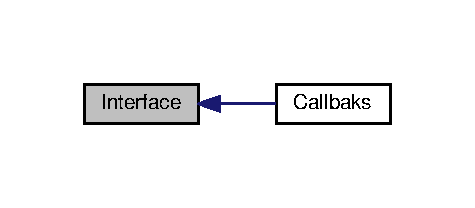
\includegraphics[width=228pt]{group___i_r_c_interface}
\end{center}
\end{figure}
\subsection*{Modules}
\begin{DoxyCompactItemize}
\item 
\hyperlink{group___i_r_c_interface_callbacks}{Callbaks}
\end{DoxyCompactItemize}


\subsection{Detailed Description}

\hypertarget{group___i_r_c_interface_callbacks}{}\section{Callbaks}
\label{group___i_r_c_interface_callbacks}\index{Callbaks@{Callbaks}}
Collaboration diagram for Callbaks\+:
% FIG 0
Funciones que van a ser llamadas desde el interface y que deben ser implementadas por el usuario. Todas estas funciones pertenecen al hilo del interfaz.

El programador puede, por supuesto, separar todas estas funciones en múltiples ficheros a efectos de desarrollo y modularización.



 \hypertarget{IRCInterface_ActivateChannelKey}{}\subsubsection{I\+R\+C\+Interface\+\_\+\+Activate\+Channel\+Key}\label{IRCInterface_ActivateChannelKey}
Llamada por el botón de activación de la clave del canal.


\begin{DoxyCode}
\textcolor{preprocessor}{#include <redes2/ircxchat.h>}

\textcolor{keywordtype}{void} \hyperlink{xchat2_8c_a33f80a29a744e4182b29e23f13c1f05c}{IRCInterface\_ActivateChannelKey} (\textcolor{keywordtype}{char} *channel, \textcolor{keywordtype}{char} * key)
\end{DoxyCode}


Llamada por el botón de activación de la clave del canal. El segundo parámetro es la clave del canal que se desea poner. Si es N\+U\+LL deberá impedirse la activación con la función implementada a tal efecto. En cualquier caso sólo se puede realizar si el servidor acepta la orden. Las strings recibidas no deben ser manipuladas por el programador, sólo leídas.


\begin{DoxyParams}[1]{Parameters}
\mbox{\tt in}  & {\em channel} & canal sobre el que se va a activar la clave. \\
\hline
\mbox{\tt in}  & {\em key} & clave para el canal indicado.\\
\hline
\end{DoxyParams}
\begin{DoxyWarning}{Warning}
Esta función debe ser implementada por el alumno.
\end{DoxyWarning}
\begin{DoxyAuthor}{Author}
Eloy Anguiano (\href{mailto:eloy.anguiano@uam.es}{\tt eloy.\+anguiano@uam.\+es})
\end{DoxyAuthor}


 \hypertarget{IRCInterface_ActivateExternalMessages}{}\subsubsection{I\+R\+C\+Interface\+\_\+\+Activate\+External\+Messages}\label{IRCInterface_ActivateExternalMessages}
Llamada por el botón de activación de la recepción de mensajes externos.


\begin{DoxyCode}
\textcolor{preprocessor}{#include <redes2/ircxchat.h>}

\textcolor{keywordtype}{void} \hyperlink{xchat2_8c_a7a439929c246e342ae525139b2c39f5d}{IRCInterface\_ActivateExternalMessages} (\textcolor{keywordtype}{char} *channel)
\end{DoxyCode}


Llamada por el botón de activación de la recepción de mensajes externos.

En cualquier caso sólo se puede realizar si el servidor acepta la orden. La string recibida no debe ser manipulada por el programador, sólo leída.


\begin{DoxyParams}[1]{Parameters}
\mbox{\tt in}  & {\em channel} & canal sobre el que se activará la recepción de mensajes externos.\\
\hline
\end{DoxyParams}
\begin{DoxyWarning}{Warning}
Esta función debe ser implementada por el alumno.
\end{DoxyWarning}
\begin{DoxyAuthor}{Author}
Eloy Anguiano (\href{mailto:eloy.anguiano@uam.es}{\tt eloy.\+anguiano@uam.\+es})
\end{DoxyAuthor}


 \hypertarget{IRCInterface_ActivateInvite}{}\subsubsection{I\+R\+C\+Interface\+\_\+\+Activate\+Invite}\label{IRCInterface_ActivateInvite}
Llamada por el botón de activación de canal de sólo invitación.


\begin{DoxyCode}
\textcolor{preprocessor}{#include <redes2/ircxchat.h>}

\textcolor{keywordtype}{void} \hyperlink{xchat2_8c_ac72762ab1e3575b421b967241db23f9c}{IRCInterface\_ActivateInvite} (\textcolor{keywordtype}{char} *channel)
\end{DoxyCode}


Llamada por el botón de activación de canal de sólo invitación.

En cualquier caso sólo se puede realizar si el servidor acepta la orden. La string recibida no debe ser manipulada por el programador, sólo leída.


\begin{DoxyParams}[1]{Parameters}
\mbox{\tt in}  & {\em channel} & canal sobre el que se activará la invitación.\\
\hline
\end{DoxyParams}
\begin{DoxyWarning}{Warning}
Esta función debe ser implementada por el alumno.
\end{DoxyWarning}
\begin{DoxyAuthor}{Author}
Eloy Anguiano (\href{mailto:eloy.anguiano@uam.es}{\tt eloy.\+anguiano@uam.\+es})
\end{DoxyAuthor}


 \hypertarget{IRCInterface_ActivateModerated}{}\subsubsection{I\+R\+C\+Interface\+\_\+\+Activate\+Moderated}\label{IRCInterface_ActivateModerated}
Llamada por el botón de activación de la moderación del canal.


\begin{DoxyCode}
\textcolor{preprocessor}{#include <redes2/ircxchat.h>}

\textcolor{keywordtype}{void} \hyperlink{xchat2_8c_af83498f4058311f4562c43a9b70566b2}{IRCInterface\_ActivateModerated} (\textcolor{keywordtype}{char} *channel)
\end{DoxyCode}


Llamada por el botón de activación de la moderación del canal.

En cualquier caso sólo se puede realizar si el servidor acepta la orden. La string recibida no debe ser manipulada por el programador, sólo leída.


\begin{DoxyParams}[1]{Parameters}
\mbox{\tt in}  & {\em channel} & canal sobre el que se activará la moderación.\\
\hline
\end{DoxyParams}
\begin{DoxyWarning}{Warning}
Esta función debe ser implementada por el alumno.
\end{DoxyWarning}
\begin{DoxyAuthor}{Author}
Eloy Anguiano (\href{mailto:eloy.anguiano@uam.es}{\tt eloy.\+anguiano@uam.\+es})
\end{DoxyAuthor}


 \hypertarget{IRCInterface_ActivateNicksLimit}{}\subsubsection{I\+R\+C\+Interface\+\_\+\+Activate\+Nicks\+Limit}\label{IRCInterface_ActivateNicksLimit}
Llamada por el botón de activación del límite de usuarios en el canal.


\begin{DoxyCode}
\textcolor{preprocessor}{#include <redes2/ircxchat.h>}

\textcolor{keywordtype}{void} \hyperlink{xchat2_8c_ab5694cc413472173bfcaa969c7d9800e}{IRCInterface\_ActivateNicksLimit} (\textcolor{keywordtype}{char} *channel, \textcolor{keywordtype}{int} * limit)
\end{DoxyCode}


Llamada por el botón de activación del límite de usuarios en el canal. El segundo es el límite de usuarios que se desea poner. Si el valor es 0 se sobrentiende que se desea eliminar este límite.

En cualquier caso sólo se puede realizar si el servidor acepta la orden. La string recibida no debe ser manipulada por el programador, sólo leída.


\begin{DoxyParams}[1]{Parameters}
\mbox{\tt in}  & {\em channel} & canal sobre el que se activará el límite de usuarios. \\
\hline
\mbox{\tt in}  & {\em limit} & límite de usuarios en el canal indicado.\\
\hline
\end{DoxyParams}
\begin{DoxyWarning}{Warning}
Esta función debe ser implementada por el alumno.
\end{DoxyWarning}
\begin{DoxyAuthor}{Author}
Eloy Anguiano (\href{mailto:eloy.anguiano@uam.es}{\tt eloy.\+anguiano@uam.\+es})
\end{DoxyAuthor}


 \hypertarget{IRCInterface_ActivatePrivate}{}\subsubsection{I\+R\+C\+Interface\+\_\+\+Activate\+Private}\label{IRCInterface_ActivatePrivate}
Llamada por el botón de activación del modo privado.


\begin{DoxyCode}
\textcolor{preprocessor}{#include <redes2/ircxchat.h>}

\textcolor{keywordtype}{void} \hyperlink{xchat2_8c_ab1f09c737c7c109a97e22de6072d731d}{IRCInterface\_ActivatePrivate} (\textcolor{keywordtype}{char} *channel)
\end{DoxyCode}


Llamada por el botón de activación del modo privado.

En cualquier caso sólo se puede realizar si el servidor acepta la orden. La string recibida no debe ser manipulada por el programador, sólo leída.


\begin{DoxyParams}[1]{Parameters}
\mbox{\tt in}  & {\em channel} & canal sobre el que se va a activar la privacidad.\\
\hline
\end{DoxyParams}
\begin{DoxyWarning}{Warning}
Esta función debe ser implementada por el alumno.
\end{DoxyWarning}
\begin{DoxyAuthor}{Author}
Eloy Anguiano (\href{mailto:eloy.anguiano@uam.es}{\tt eloy.\+anguiano@uam.\+es})
\end{DoxyAuthor}


 \hypertarget{IRCInterface_ActivateProtectTopic}{}\subsubsection{I\+R\+C\+Interface\+\_\+\+Activate\+Protect\+Topic}\label{IRCInterface_ActivateProtectTopic}
Llamada por el botón de activación de la protección de tópico.


\begin{DoxyCode}
\textcolor{preprocessor}{#include <redes2/ircxchat.h>}

\textcolor{keywordtype}{void} \hyperlink{xchat2_8c_ac45f12d4dcacf3b5485eec6fdc51df93}{IRCInterface\_ActivateProtectTopic} (\textcolor{keywordtype}{char} *channel)
\end{DoxyCode}


Llamada por el botón de activación de la protección de tópico.

En cualquier caso sólo se puede realizar si el servidor acepta la orden. La string recibida no debe ser manipulada por el programador, sólo leída.


\begin{DoxyParams}[1]{Parameters}
\mbox{\tt in}  & {\em channel} & canal sobre el que se va a activar la protección de tópico.\\
\hline
\end{DoxyParams}
\begin{DoxyWarning}{Warning}
Esta función debe ser implementada por el alumno.
\end{DoxyWarning}
\begin{DoxyAuthor}{Author}
Eloy Anguiano (\href{mailto:eloy.anguiano@uam.es}{\tt eloy.\+anguiano@uam.\+es})
\end{DoxyAuthor}


 \hypertarget{IRCInterface_ActivateSecret}{}\subsubsection{I\+R\+C\+Interface\+\_\+\+Activate\+Secret}\label{IRCInterface_ActivateSecret}
Llamada por el botón de activación de canal secreto.


\begin{DoxyCode}
\textcolor{preprocessor}{#include <redes2/ircxchat.h>}

\textcolor{keywordtype}{void} \hyperlink{xchat2_8c_aa9e9155115b834d85a4d10cb27f99093}{IRCInterface\_ActivateSecret} (\textcolor{keywordtype}{char} *channel)
\end{DoxyCode}


Llamada por el botón de activación de canal secreto.

En cualquier caso sólo se puede realizar si el servidor acepta la orden. La string recibida no debe ser manipulada por el programador, sólo leída.


\begin{DoxyParams}[1]{Parameters}
\mbox{\tt in}  & {\em channel} & canal sobre el que se va a activar el estado de secreto.\\
\hline
\end{DoxyParams}
\begin{DoxyWarning}{Warning}
Esta función debe ser implementada por el alumno.
\end{DoxyWarning}
\begin{DoxyAuthor}{Author}
Eloy Anguiano (\href{mailto:eloy.anguiano@uam.es}{\tt eloy.\+anguiano@uam.\+es})
\end{DoxyAuthor}


 \hypertarget{IRCInterface_BanNick}{}\subsubsection{I\+R\+C\+Interface\+\_\+\+Ban\+Nick}\label{IRCInterface_BanNick}
Llamada por el botón \char`\"{}\+Banear\char`\"{}.


\begin{DoxyCode}
\textcolor{preprocessor}{#include <redes2/ircxchat.h>}

\textcolor{keywordtype}{void} \hyperlink{xchat2_8c_a42773b5a840f9d0455f148d285e1e595}{IRCInterface\_BanNick} (\textcolor{keywordtype}{char} *channel, \textcolor{keywordtype}{char} *nick)
\end{DoxyCode}


Llamada por el botón \char`\"{}\+Banear\char`\"{}. Previamente debe seleccionarse un nick del canal para darle voz a dicho usuario.

En cualquier caso sólo se puede realizar si el servidor acepta la orden. Las strings recibidas no deben ser manipuladas por el programador, sólo leídas.


\begin{DoxyParams}[1]{Parameters}
\mbox{\tt in}  & {\em channel} & canal sobre el que se va a realizar el baneo. En principio es un valor innecesario. \\
\hline
\mbox{\tt in}  & {\em nick} & nick del usuario que va a ser baneado\\
\hline
\end{DoxyParams}
\begin{DoxyWarning}{Warning}
Esta función debe ser implementada por el alumno.
\end{DoxyWarning}
\begin{DoxyAuthor}{Author}
Eloy Anguiano (\href{mailto:eloy.anguiano@uam.es}{\tt eloy.\+anguiano@uam.\+es})
\end{DoxyAuthor}


 \hypertarget{IRCInterface_Connect}{}\subsubsection{I\+R\+C\+Interface\+\_\+\+Connect}\label{IRCInterface_Connect}
Llamada por los distintos botones de conexión.


\begin{DoxyCode}
\textcolor{preprocessor}{#include <redes2/ircxchat.h>}

\textcolor{keywordtype}{long} \hyperlink{xchat2_8c_aed072f4ce0d6e90697d4d6eb0278a2ad}{IRCInterface\_Connect} (\textcolor{keywordtype}{char} *nick, \textcolor{keywordtype}{char} * user, \textcolor{keywordtype}{char} * realname, \textcolor{keywordtype}{char} * password, \textcolor{keywordtype}{
      char} * server, \textcolor{keywordtype}{int} port, \textcolor{keywordtype}{boolean} ssl)
\end{DoxyCode}


Función a implementar por el programador. Llamada por los distintos botones de conexión. Si implementará la comunicación completa, incluido el registro del usuario en el servidor.

En cualquier caso sólo se puede realizar si el servidor acepta la orden. Las strings recibidas no deben ser manipuladas por el programador, sólo leída.


\begin{DoxyParams}[1]{Parameters}
\mbox{\tt in}  & {\em nick} & nick con el que se va a realizar la conexíón. \\
\hline
\mbox{\tt in}  & {\em user} & usuario con el que se va a realizar la conexión. \\
\hline
\mbox{\tt in}  & {\em realname} & nombre real con el que se va a realizar la conexión. \\
\hline
\mbox{\tt in}  & {\em password} & password del usuario si es necesaria, puede valer N\+U\+LL. \\
\hline
\mbox{\tt in}  & {\em server} & nombre o ip del servidor con el que se va a realizar la conexión. \\
\hline
\mbox{\tt in}  & {\em port} & puerto del servidor con el que se va a realizar la conexión. \\
\hline
\mbox{\tt in}  & {\em ssl} & puede ser T\+R\+UE si la conexión tiene que ser segura y F\+A\+L\+SE si no es así.\\
\hline
\end{DoxyParams}

\begin{DoxyRetVals}{Return values}
{\em I\+R\+C\+\_\+\+OK} & si todo ha sido correcto (debe devolverlo). \\
\hline
{\em I\+R\+C\+E\+R\+R\+\_\+\+N\+O\+S\+SL} & si el valor de S\+SL es T\+R\+UE y no se puede activar la conexión S\+SL pero sí una conexión no protegida (debe devolverlo). \\
\hline
{\em I\+R\+C\+E\+R\+R\+\_\+\+N\+O\+C\+O\+N\+N\+E\+CT} & en caso de que no se pueda realizar la comunicación (debe devolverlo).\\
\hline
\end{DoxyRetVals}
\begin{DoxyWarning}{Warning}
Esta función debe ser implementada por el alumno.
\end{DoxyWarning}
\begin{DoxyAuthor}{Author}
Eloy Anguiano (\href{mailto:eloy.anguiano@uam.es}{\tt eloy.\+anguiano@uam.\+es})
\end{DoxyAuthor}


 \hypertarget{IRCInterface_DeactivateChannelKey}{}\subsubsection{I\+R\+C\+Interface\+\_\+\+Deactivate\+Channel\+Key}\label{IRCInterface_DeactivateChannelKey}
Llamada por el botón de desactivación de la clave del canal.


\begin{DoxyCode}
\textcolor{preprocessor}{#include <redes2/ircxchat.h>}

\textcolor{keywordtype}{void} \hyperlink{xchat2_8c_a3e67ee0cd384b524d57fda14593dce8e}{IRCInterface\_DeactivateChannelKey} (\textcolor{keywordtype}{char} *channel)
\end{DoxyCode}


Llamada por el botón de desactivación de la clave del canal.

En cualquier caso sólo se puede realizar si el servidor acepta la orden. La string recibida no debe ser manipulada por el programador, sólo leída.


\begin{DoxyParams}[1]{Parameters}
\mbox{\tt in}  & {\em channel} & canal sobre el que se va a desactivar la clave.\\
\hline
\end{DoxyParams}
\begin{DoxyWarning}{Warning}
Esta función debe ser implementada por el alumno.
\end{DoxyWarning}
\begin{DoxyAuthor}{Author}
Eloy Anguiano (\href{mailto:eloy.anguiano@uam.es}{\tt eloy.\+anguiano@uam.\+es})
\end{DoxyAuthor}


 \hypertarget{IRCInterface_DeactivateExternalMessages}{}\subsubsection{I\+R\+C\+Interface\+\_\+\+Deactivate\+External\+Messages}\label{IRCInterface_DeactivateExternalMessages}
Llamada por el botón de desactivación de la recepción de mensajes externos.


\begin{DoxyCode}
\textcolor{preprocessor}{#include <redes2/ircxchat.h>}

\textcolor{keywordtype}{void} \hyperlink{xchat2_8c_a638b1535f4ecbc9a6affb2df2a6a946e}{IRCInterface\_DeactivateExternalMessages} (\textcolor{keywordtype}{char} *channel)
\end{DoxyCode}


Llamada por el botón de desactivación de la recepción de mensajes externos.

En cualquier caso sólo se puede realizar si el servidor acepta la orden. La string recibida no debe ser manipulada por el programador, sólo leída.


\begin{DoxyParams}[1]{Parameters}
\mbox{\tt in}  & {\em channel} & canal sobre el que se va a deactivar la recepción de mensajes externos.\\
\hline
\end{DoxyParams}
\begin{DoxyWarning}{Warning}
Esta función debe ser implementada por el alumno.
\end{DoxyWarning}
\begin{DoxyAuthor}{Author}
Eloy Anguiano (\href{mailto:eloy.anguiano@uam.es}{\tt eloy.\+anguiano@uam.\+es})
\end{DoxyAuthor}


 \hypertarget{IRCInterface_DeactivateInvite}{}\subsubsection{I\+R\+C\+Interface\+\_\+\+Deactivate\+Invite}\label{IRCInterface_DeactivateInvite}
Llamada por el botón de desactivación de canal de sólo invitación.


\begin{DoxyCode}
\textcolor{preprocessor}{#include <redes2/ircxchat.h>}

\textcolor{keywordtype}{void} \hyperlink{xchat2_8c_a9ba4e98a3729737aa63ebec54ba4e894}{IRCInterface\_DeactivateInvite} (\textcolor{keywordtype}{char} *channel)
\end{DoxyCode}


Llamada por el botón de desactivación de canal de sólo invitación.

En cualquier caso sólo se puede realizar si el servidor acepta la orden. La string recibida no debe ser manipulada por el programador, sólo leída.


\begin{DoxyParams}[1]{Parameters}
\mbox{\tt in}  & {\em channel} & canal sobre el que se va a desactivar la invitación.\\
\hline
\end{DoxyParams}
\begin{DoxyWarning}{Warning}
Esta función debe ser implementada por el alumno.
\end{DoxyWarning}
\begin{DoxyAuthor}{Author}
Eloy Anguiano (\href{mailto:eloy.anguiano@uam.es}{\tt eloy.\+anguiano@uam.\+es})
\end{DoxyAuthor}


 \hypertarget{IRCInterface_DeactivateModerated}{}\subsubsection{I\+R\+C\+Interface\+\_\+\+Deactivate\+Moderated}\label{IRCInterface_DeactivateModerated}
Llamada por el botón de desactivación de la moderación del canal.


\begin{DoxyCode}
\textcolor{preprocessor}{#include <redes2/ircxchat.h>}

\textcolor{keywordtype}{void} \hyperlink{xchat2_8c_ab760e8144b38f6c14bd809d157cee5d4}{IRCInterface\_DeactivateModerated} (\textcolor{keywordtype}{char} *channel)
\end{DoxyCode}


Llamada por el botón de desactivación de la moderación del canal.

En cualquier caso sólo se puede realizar si el servidor acepta la orden. La string recibida no debe ser manipulada por el programador, sólo leída.


\begin{DoxyParams}[1]{Parameters}
\mbox{\tt in}  & {\em channel} & canal sobre el que se va a desactivar la moderación.\\
\hline
\end{DoxyParams}
\begin{DoxyWarning}{Warning}
Esta función debe ser implementada por el alumno.
\end{DoxyWarning}
\begin{DoxyAuthor}{Author}
Eloy Anguiano (\href{mailto:eloy.anguiano@uam.es}{\tt eloy.\+anguiano@uam.\+es})
\end{DoxyAuthor}


 \hypertarget{IRCInterface_DeactivateNicksLimit}{}\subsubsection{I\+R\+C\+Interface\+\_\+\+Deactivate\+Nicks\+Limit}\label{IRCInterface_DeactivateNicksLimit}
Llamada por el botón de desactivación de la protección de tópico.


\begin{DoxyCode}
\textcolor{preprocessor}{#include <redes2/ircxchat.h>}

\textcolor{keywordtype}{void} \hyperlink{xchat2_8c_a92c8cfbe2e14e19277e1c97d11719e80}{IRCInterface\_DeactivateNicksLimit} (\textcolor{keywordtype}{char} *channel)
\end{DoxyCode}


Llamada por el botón de desactivación del límite de usuarios en el canal.

En cualquier caso sólo se puede realizar si el servidor acepta la orden. La string recibida no debe ser manipulada por el programador, sólo leída.


\begin{DoxyParams}[1]{Parameters}
\mbox{\tt in}  & {\em channel} & canal sobre el que se va a desactivar el límite de usuarios.\\
\hline
\end{DoxyParams}
\begin{DoxyWarning}{Warning}
Esta función debe ser implementada por el alumno.
\end{DoxyWarning}
\begin{DoxyAuthor}{Author}
Eloy Anguiano (\href{mailto:eloy.anguiano@uam.es}{\tt eloy.\+anguiano@uam.\+es})
\end{DoxyAuthor}


 \hypertarget{IRCInterface_DeactivatePrivate}{}\subsubsection{I\+R\+C\+Interface\+\_\+\+Deactivate\+Private}\label{IRCInterface_DeactivatePrivate}
Llamada por el botón de desactivación del modo privado.


\begin{DoxyCode}
\textcolor{preprocessor}{#include <redes2/ircxchat.h>}

\textcolor{keywordtype}{void} \hyperlink{xchat2_8c_a8a6141803691ba327f11ba763ad075d4}{IRCInterface\_DeactivatePrivate} (\textcolor{keywordtype}{char} *channel)
\end{DoxyCode}


Llamada por el botón de desactivación del modo privado.

En cualquier caso sólo se puede realizar si el servidor acepta la orden. La string recibida no debe ser manipulada por el programador, sólo leída.

\begin{DoxyWarning}{Warning}
Esta función debe ser implementada por el alumno.
\end{DoxyWarning}

\begin{DoxyParams}[1]{Parameters}
\mbox{\tt in}  & {\em channel} & canal sobre el que se va a desactivar la privacidad.\\
\hline
\end{DoxyParams}
\begin{DoxyWarning}{Warning}
Esta función debe ser implementada por el alumno.
\end{DoxyWarning}
\begin{DoxyAuthor}{Author}
Eloy Anguiano (\href{mailto:eloy.anguiano@uam.es}{\tt eloy.\+anguiano@uam.\+es})
\end{DoxyAuthor}


 \hypertarget{IRCInterface_DeactivateProtectTopic}{}\subsubsection{I\+R\+C\+Interface\+\_\+\+Deactivate\+Protect\+Topic}\label{IRCInterface_DeactivateProtectTopic}
Llamada por el botón de desactivación de la protección de tópico.


\begin{DoxyCode}
\textcolor{preprocessor}{#include <redes2/ircxchat.h>}

\textcolor{keywordtype}{void} \hyperlink{xchat2_8c_a5a57541a950f8c2c40b4b44c32b28ed9}{IRCInterface\_DeactivateProtectTopic} (\textcolor{keywordtype}{char} *channel)
\end{DoxyCode}


Llamada por el botón de desactivación de la protección de tópico.

En cualquier caso sólo se puede realizar si el servidor acepta la orden. La string recibida no debe ser manipulada por el programador, sólo leída.


\begin{DoxyParams}[1]{Parameters}
\mbox{\tt in}  & {\em channel} & canal sobre el que se va a desactivar la protección de tópico.\\
\hline
\end{DoxyParams}
\begin{DoxyWarning}{Warning}
Esta función debe ser implementada por el alumno.
\end{DoxyWarning}
\begin{DoxyAuthor}{Author}
Eloy Anguiano (\href{mailto:eloy.anguiano@uam.es}{\tt eloy.\+anguiano@uam.\+es})
\end{DoxyAuthor}


 \hypertarget{IRCInterface_DeactivateSecret}{}\subsubsection{I\+R\+C\+Interface\+\_\+\+Deactivate\+Secret}\label{IRCInterface_DeactivateSecret}
Llamada por el botón de desactivación de canal secreto.


\begin{DoxyCode}
\textcolor{preprocessor}{#include <redes2/ircxchat.h>}

\textcolor{keywordtype}{void} \hyperlink{xchat2_8c_a4956427664cabc7d5b2bd1589a207324}{IRCInterface\_DeactivateSecret} (\textcolor{keywordtype}{char} *channel)
\end{DoxyCode}


Llamada por el botón de desactivación de canal secreto.

En cualquier caso sólo se puede realizar si el servidor acepta la orden. La string recibida no debe ser manipulada por el programador, sólo leída.


\begin{DoxyParams}[1]{Parameters}
\mbox{\tt in}  & {\em channel} & canal sobre el que se va a desactivar la propiedad de canal secreto.\\
\hline
\end{DoxyParams}
\begin{DoxyWarning}{Warning}
Esta función debe ser implementada por el alumno.
\end{DoxyWarning}
\begin{DoxyAuthor}{Author}
Eloy Anguiano (\href{mailto:eloy.anguiano@uam.es}{\tt eloy.\+anguiano@uam.\+es})
\end{DoxyAuthor}


 \hypertarget{IRCInterface_DisconnectServer}{}\subsubsection{I\+R\+C\+Interface\+\_\+\+Disconnect\+Server}\label{IRCInterface_DisconnectServer}
Llamada por los distintos botones de desconexión.


\begin{DoxyCode}
\textcolor{preprocessor}{#include <redes2/ircxchat.h>}

\textcolor{keywordtype}{boolean} \hyperlink{xchat2_8c_a8bf0424ef7f845be79a056e9aed56fe2}{IRCInterface\_DisconnectServer} (\textcolor{keywordtype}{char} * server, \textcolor{keywordtype}{int} port)
\end{DoxyCode}


Llamada por los distintos botones de desconexión. Debe cerrar la conexión con el servidor.

En cualquier caso sólo se puede realizar si el servidor acepta la orden. La string recibida no debe ser manipulada por el programador, sólo leída.


\begin{DoxyParams}[1]{Parameters}
\mbox{\tt in}  & {\em server} & nombre o ip del servidor del que se va a realizar la desconexión. \\
\hline
\mbox{\tt in}  & {\em port} & puerto sobre el que se va a realizar la desconexión.\\
\hline
\end{DoxyParams}

\begin{DoxyRetVals}{Return values}
{\em T\+R\+UE} & si se ha cerrado la conexión (debe devolverlo). \\
\hline
{\em F\+A\+L\+SE} & en caso contrario (debe devolverlo).\\
\hline
\end{DoxyRetVals}
\begin{DoxyWarning}{Warning}
Esta función debe ser implementada por el alumno.
\end{DoxyWarning}
\begin{DoxyAuthor}{Author}
Eloy Anguiano (\href{mailto:eloy.anguiano@uam.es}{\tt eloy.\+anguiano@uam.\+es})
\end{DoxyAuthor}


 \hypertarget{IRCInterface_ExitAudioChat}{}\subsubsection{I\+R\+C\+Interface\+\_\+\+Exit\+Audio\+Chat}\label{IRCInterface_ExitAudioChat}
Llamada por el botón \char`\"{}\+Cancelar\char`\"{} del diálogo de chat de voz.


\begin{DoxyCode}
\textcolor{preprocessor}{#include <redes2/ircxchat.h>}

\textcolor{keywordtype}{void} \hyperlink{xchat2_8c_ab431412191716f751461f94d613ffdab}{IRCInterface\_ExitAudioChat} (\textcolor{keywordtype}{char} *nick)
\end{DoxyCode}


Llamada por el botón \char`\"{}\+Parar\char`\"{} del diálogo de chat de voz. Previamente debe seleccionarse un nick del canal para darle voz a dicho usuario. Esta función cierrala comunicación. Evidentemente tiene que actuar sobre el hilo de chat de voz.

En cualquier caso sólo se puede realizar si el servidor acepta la orden. La string recibida no debe ser manipulada por el programador, sólo leída.


\begin{DoxyParams}[1]{Parameters}
\mbox{\tt in}  & {\em nick} & nick del usuario que solicita la parada del chat de audio.\\
\hline
\end{DoxyParams}

\begin{DoxyRetVals}{Return values}
{\em T\+R\+UE} & si se ha cerrado la comunicación (debe devolverlo). \\
\hline
{\em F\+A\+L\+SE} & en caso contrario (debe devolverlo).\\
\hline
\end{DoxyRetVals}
\begin{DoxyWarning}{Warning}
Esta función debe ser implementada por el alumno.
\end{DoxyWarning}
\begin{DoxyAuthor}{Author}
Eloy Anguiano (\href{mailto:eloy.anguiano@uam.es}{\tt eloy.\+anguiano@uam.\+es})
\end{DoxyAuthor}


 \hypertarget{IRCInterface_GiveOp}{}\subsubsection{I\+R\+C\+Interface\+\_\+\+Give\+Op}\label{IRCInterface_GiveOp}
Llamada por el botón \char`\"{}\+Op\char`\"{}.


\begin{DoxyCode}
\textcolor{preprocessor}{#include <redes2/ircxchat.h>}

\textcolor{keywordtype}{void} \hyperlink{xchat2_8c_ae075029bb55e8b995f22beb0810674f4}{IRCInterface\_GiveOp} (\textcolor{keywordtype}{char} *channel, \textcolor{keywordtype}{char} *nick)
\end{DoxyCode}


Llamada por el botón \char`\"{}\+Op\char`\"{}. Previamente debe seleccionarse un nick del canal para darle \char`\"{}op\char`\"{} a dicho usuario.

En cualquier caso sólo se puede realizar si el servidor acepta la orden. Las strings recibidas no deben ser manipuladas por el programador, sólo leídas.


\begin{DoxyParams}[1]{Parameters}
\mbox{\tt in}  & {\em channel} & canal sobre el que se va dar op al usuario. \\
\hline
\mbox{\tt in}  & {\em nick} & nick al que se le va a dar el nivel de op.\\
\hline
\end{DoxyParams}
\begin{DoxyWarning}{Warning}
Esta función debe ser implementada por el alumno.
\end{DoxyWarning}
\begin{DoxyAuthor}{Author}
Eloy Anguiano (\href{mailto:eloy.anguiano@uam.es}{\tt eloy.\+anguiano@uam.\+es})
\end{DoxyAuthor}


 \hypertarget{IRCInterface_GiveVoice}{}\subsubsection{I\+R\+C\+Interface\+\_\+\+Give\+Voice}\label{IRCInterface_GiveVoice}
Llamada por el botón \char`\"{}\+Dar voz\char`\"{}.


\begin{DoxyCode}
\textcolor{preprocessor}{#include <redes2/ircxchat.h>}

\textcolor{keywordtype}{void} \hyperlink{xchat2_8c_ae9effb4bdaf4a2cdf2dd9edbeb90b430}{IRCInterface\_GiveVoice} (\textcolor{keywordtype}{char} *channel, \textcolor{keywordtype}{char} *nick)
\end{DoxyCode}


Llamada por el botón \char`\"{}\+Dar voz\char`\"{}. Previamente debe seleccionarse un nick del canal para darle voz a dicho usuario.

En cualquier caso sólo se puede realizar si el servidor acepta la orden. Las strings recibidas no deben ser manipuladas por el programador, sólo leídas.


\begin{DoxyParams}[1]{Parameters}
\mbox{\tt in}  & {\em channel} & canal sobre el que se va dar voz al usuario. \\
\hline
\mbox{\tt in}  & {\em nick} & nick al que se le va a dar voz.\\
\hline
\end{DoxyParams}
\begin{DoxyWarning}{Warning}
Esta función debe ser implementada por el alumno.
\end{DoxyWarning}
\begin{DoxyAuthor}{Author}
Eloy Anguiano (\href{mailto:eloy.anguiano@uam.es}{\tt eloy.\+anguiano@uam.\+es})
\end{DoxyAuthor}


 \hypertarget{IRCInterface_KickNick}{}\subsubsection{I\+R\+C\+Interface\+\_\+\+Kick\+Nick}\label{IRCInterface_KickNick}
Llamada por el botón \char`\"{}\+Echar\char`\"{}.


\begin{DoxyCode}
\textcolor{preprocessor}{#include <redes2/ircxchat.h>}

\textcolor{keywordtype}{void} \hyperlink{xchat2_8c_a7adfea400a96160585f86179bafb055f}{IRCInterface\_KickNick} (\textcolor{keywordtype}{char} *channel, \textcolor{keywordtype}{char} *nick)
\end{DoxyCode}


Llamada por el botón \char`\"{}\+Echar\char`\"{}. Previamente debe seleccionarse un nick del canal para darle voz a dicho usuario.

En cualquier caso sólo se puede realizar si el servidor acepta la orden. Las strings recibidas no deben ser manipuladas por el programador, sólo leídas.


\begin{DoxyParams}[1]{Parameters}
\mbox{\tt in}  & {\em channel} & canal sobre el que se va a expulsar al usuario. \\
\hline
\mbox{\tt in}  & {\em nick} & nick del usuario que va a ser expulsado.\\
\hline
\end{DoxyParams}
\begin{DoxyWarning}{Warning}
Esta función debe ser implementada por el alumno.
\end{DoxyWarning}
\begin{DoxyAuthor}{Author}
Eloy Anguiano (\href{mailto:eloy.anguiano@uam.es}{\tt eloy.\+anguiano@uam.\+es})
\end{DoxyAuthor}


 \hypertarget{IRCInterface_NewCommandText}{}\subsubsection{I\+R\+C\+Interface\+\_\+\+New\+Command\+Text}\label{IRCInterface_NewCommandText}
Llamada la tecla E\+N\+T\+ER en el campo de texto y comandos.


\begin{DoxyCode}
\textcolor{preprocessor}{#include <redes2/ircxchat.h>}

\textcolor{keywordtype}{void} \hyperlink{xchat2_8c_a214e10b19c8be028fb35d2a7abf3f798}{IRCInterface\_NewCommandText} (\textcolor{keywordtype}{char} *command)
\end{DoxyCode}


Llamada de la tecla E\+N\+T\+ER en el campo de texto y comandos. El texto deberá ser enviado y el comando procesado por las funciones de \char`\"{}parseo\char`\"{} de comandos de usuario.

En cualquier caso sólo se puede realizar si el servidor acepta la orden. La string recibida no debe ser manipulada por el programador, sólo leída.


\begin{DoxyParams}[1]{Parameters}
\mbox{\tt in}  & {\em comando} & introducido por el usuario.\\
\hline
\end{DoxyParams}
\begin{DoxyWarning}{Warning}
Esta función debe ser implementada por el alumno.
\end{DoxyWarning}
\begin{DoxyAuthor}{Author}
Eloy Anguiano (\href{mailto:eloy.anguiano@uam.es}{\tt eloy.\+anguiano@uam.\+es})
\end{DoxyAuthor}


 \hypertarget{IRCInterface_NewTopicEnter}{}\subsubsection{I\+R\+C\+Interface\+\_\+\+New\+Topic\+Enter}\label{IRCInterface_NewTopicEnter}
Llamada cuando se pulsa la tecla E\+N\+T\+ER en el campo de tópico.


\begin{DoxyCode}
\textcolor{preprocessor}{#include <redes2/ircxchat.h>}

\textcolor{keywordtype}{void} \hyperlink{xchat2_8c_a080cf34ff506481737f6d08af60ca92b}{IRCInterface\_NewTopicEnter} (\textcolor{keywordtype}{char} * topicdata)
\end{DoxyCode}


Llamada cuando se pulsa la tecla E\+N\+T\+ER en el campo de tópico. Deberá intentarse cambiar el tópico del canal.

En cualquier caso sólo se puede realizar si el servidor acepta la orden. La string recibida no debe ser manipulada por el programador, sólo leída.

param\mbox{[}in\mbox{]} topicdata string con el tópico que se desea poner en el canal.

\begin{DoxyWarning}{Warning}
Esta función debe ser implementada por el alumno.
\end{DoxyWarning}
\begin{DoxyAuthor}{Author}
Eloy Anguiano (\href{mailto:eloy.anguiano@uam.es}{\tt eloy.\+anguiano@uam.\+es})
\end{DoxyAuthor}


 \hypertarget{IRCInterface_SendFile}{}\subsubsection{I\+R\+C\+Interface\+\_\+\+Send\+File}\label{IRCInterface_SendFile}
Llamada por el botón \char`\"{}\+Enviar Archivo\char`\"{}.


\begin{DoxyCode}
\textcolor{preprocessor}{#include <redes2/ircxchat.h>}

\textcolor{keywordtype}{void} \hyperlink{xchat2_8c_a100f1c87bb3b399a7284e62dd2e6172a}{IRCInterface\_SendFile} (\textcolor{keywordtype}{char} * filename, \textcolor{keywordtype}{char} *nick, \textcolor{keywordtype}{char} *data, \textcolor{keywordtype}{long} \textcolor{keywordtype}{unsigned} \textcolor{keywordtype}{int}
       length)
\end{DoxyCode}


Llamada por el botón \char`\"{}\+Enviar Archivo\char`\"{}. Previamente debe seleccionarse un nick del canal para darle voz a dicho usuario. Esta función como todos los demás callbacks bloquea el interface y por tanto es el programador el que debe determinar si crea un nuevo hilo para enviar el archivo o no lo hace.

En cualquier caso sólo se puede realizar si el servidor acepta la orden. Las strings recibidas no deben ser manipuladas por el programador, sólo leídas.


\begin{DoxyParams}[1]{Parameters}
\mbox{\tt in}  & {\em filename} & nombre del fichero a enviar. \\
\hline
\mbox{\tt in}  & {\em nick} & nick del usuario que enviará el fichero. \\
\hline
\mbox{\tt in}  & {\em data} & datos a ser enviados. \\
\hline
\mbox{\tt in}  & {\em length} & longitud de los datos a ser enviados.\\
\hline
\end{DoxyParams}

\begin{DoxyRetVals}{Return values}
{\em T\+R\+UE} & si se ha establecido la comunicación (debe devolverlo). \\
\hline
{\em F\+A\+L\+SE} & en caso contrario (debe devolverlo).\\
\hline
\end{DoxyRetVals}
\begin{DoxyWarning}{Warning}
Esta función debe ser implementada por el alumno.
\end{DoxyWarning}
\begin{DoxyAuthor}{Author}
Eloy Anguiano (\href{mailto:eloy.anguiano@uam.es}{\tt eloy.\+anguiano@uam.\+es})
\end{DoxyAuthor}


 \hypertarget{IRCInterface_StartAudioChat}{}\subsubsection{I\+R\+C\+Interface\+\_\+\+Start\+Audio\+Chat}\label{IRCInterface_StartAudioChat}
Llamada por el botón \char`\"{}\+Iniciar\char`\"{} del diálogo de chat de voz.


\begin{DoxyCode}
\textcolor{preprocessor}{#include <redes2/ircxchat.h>}

\textcolor{keywordtype}{void} \hyperlink{xchat2_8c_a5dc7a44587e609b416a783cd420a12e3}{IRCInterface\_StartAudioChat} (\textcolor{keywordtype}{char} *nick)
\end{DoxyCode}


Llamada por el botón \char`\"{}\+Iniciar\char`\"{} del diálogo de chat de voz. Previamente debe seleccionarse un nick del canal para darle voz a dicho usuario. Esta función como todos los demás callbacks bloquea el interface y por tanto para mantener la funcionalidad del chat de voz es imprescindible crear un hilo a efectos de comunicación de voz.

En cualquier caso sólo se puede realizar si el servidor acepta la orden. La string recibida no debe ser manipulada por el programador, sólo leída.


\begin{DoxyParams}[1]{Parameters}
\mbox{\tt in}  & {\em nick} & nick del usuario con el que se desea conectar.\\
\hline
\end{DoxyParams}

\begin{DoxyRetVals}{Return values}
{\em T\+R\+UE} & si se ha establecido la comunicación (debe devolverlo). \\
\hline
{\em F\+A\+L\+SE} & en caso contrario (debe devolverlo).\\
\hline
\end{DoxyRetVals}
\begin{DoxyWarning}{Warning}
Esta función debe ser implementada por el alumno.
\end{DoxyWarning}
\begin{DoxyAuthor}{Author}
Eloy Anguiano (\href{mailto:eloy.anguiano@uam.es}{\tt eloy.\+anguiano@uam.\+es})
\end{DoxyAuthor}


 \hypertarget{IRCInterface_StopAudioChat}{}\subsubsection{I\+R\+C\+Interface\+\_\+\+Stop\+Audio\+Chat}\label{IRCInterface_StopAudioChat}
Llamada por el botón \char`\"{}\+Parar\char`\"{} del diálogo de chat de voz.


\begin{DoxyCode}
\textcolor{preprocessor}{#include <redes2/ircxchat.h>}

\textcolor{keywordtype}{void} \hyperlink{xchat2_8c_a754a3d3dd311194637c07cc701e7d507}{IRCInterface\_StopAudioChat} (\textcolor{keywordtype}{char} *nick)
\end{DoxyCode}


Llamada por el botón \char`\"{}\+Parar\char`\"{} del diálogo de chat de voz. Previamente debe seleccionarse un nick del canal para darle voz a dicho usuario. Esta función sólo para la comunicación que puede ser reiniciada. Evidentemente tiene que actuar sobre el hilo de chat de voz.

En cualquier caso sólo se puede realizar si el servidor acepta la orden. La string recibida no debe ser manipulada por el programador, sólo leída.


\begin{DoxyParams}[1]{Parameters}
\mbox{\tt in}  & {\em nick} & nick del usuario con el que se quiere parar el chat de voz.\\
\hline
\end{DoxyParams}

\begin{DoxyRetVals}{Return values}
{\em T\+R\+UE} & si se ha parado la comunicación (debe devolverlo). \\
\hline
{\em F\+A\+L\+SE} & en caso contrario (debe devolverlo).\\
\hline
\end{DoxyRetVals}
\begin{DoxyWarning}{Warning}
Esta función debe ser implementada por el alumno.
\end{DoxyWarning}
\begin{DoxyAuthor}{Author}
Eloy Anguiano (\href{mailto:eloy.anguiano@uam.es}{\tt eloy.\+anguiano@uam.\+es})
\end{DoxyAuthor}


 \hypertarget{IRCInterface_TakeOp}{}\subsubsection{I\+R\+C\+Interface\+\_\+\+Take\+Op}\label{IRCInterface_TakeOp}
Llamada por el botón \char`\"{}\+Quitar Op\char`\"{}.


\begin{DoxyCode}
\textcolor{preprocessor}{#include <redes2/ircxchat.h>}

\textcolor{keywordtype}{void} \hyperlink{xchat2_8c_a4e2a1ea75e59306142030a91a054b7e6}{IRCInterface\_TakeOp} (\textcolor{keywordtype}{char} *channel, \textcolor{keywordtype}{char} *nick)
\end{DoxyCode}


Llamada por el botón \char`\"{}\+Quitar Op\char`\"{}. Previamente debe seleccionarse un nick del canal para quitarle \char`\"{}op\char`\"{} a dicho usuario.

En cualquier caso sólo se puede realizar si el servidor acepta la orden. Las strings recibidas no deben ser manipuladas por el programador, sólo leídas.


\begin{DoxyParams}[1]{Parameters}
\mbox{\tt in}  & {\em channel} & canal sobre el que se va a quitar op al usuario. \\
\hline
\mbox{\tt in}  & {\em nick} & nick del usuario al que se le va a quitar op.\\
\hline
\end{DoxyParams}
\begin{DoxyWarning}{Warning}
Esta función debe ser implementada por el alumno.
\end{DoxyWarning}
\begin{DoxyAuthor}{Author}
Eloy Anguiano (\href{mailto:eloy.anguiano@uam.es}{\tt eloy.\+anguiano@uam.\+es})
\end{DoxyAuthor}


 \hypertarget{IRCInterface_TakeVoice}{}\subsubsection{I\+R\+C\+Interface\+\_\+\+Take\+Voice}\label{IRCInterface_TakeVoice}
Llamada por el botón \char`\"{}\+Quitar voz\char`\"{}.


\begin{DoxyCode}
\textcolor{preprocessor}{#include <redes2/ircxchat.h>}

\textcolor{keywordtype}{void} \hyperlink{xchat2_8c_a2ff2e10ed1cb1a399293b6f76ac1e5ae}{IRCInterface\_TakeVoice} (\textcolor{keywordtype}{char} *channel, \textcolor{keywordtype}{char} *nick)
\end{DoxyCode}


Llamada por el botón \char`\"{}\+Quitar voz\char`\"{}. Previamente debe seleccionarse un nick del canal para darle voz a dicho usuario.

En cualquier caso sólo se puede realizar si el servidor acepta la orden. Las strings recibidas no deben ser manipuladas por el programador, sólo leídas.


\begin{DoxyParams}[1]{Parameters}
\mbox{\tt in}  & {\em channel} & canal sobre el que se le va a quitar voz al usuario. \\
\hline
\mbox{\tt in}  & {\em nick} & nick del usuario al que se va a quitar la voz.\\
\hline
\end{DoxyParams}
\begin{DoxyWarning}{Warning}
Esta función debe ser implementada por el alumno.
\end{DoxyWarning}
\begin{DoxyAuthor}{Author}
Eloy Anguiano (\href{mailto:eloy.anguiano@uam.es}{\tt eloy.\+anguiano@uam.\+es})
\end{DoxyAuthor}


 
\chapter{Class Documentation}
\hypertarget{struct_file__args}{\section{File\-\_\-args Struct Reference}
\label{struct_file__args}\index{File\-\_\-args@{File\-\_\-args}}
}


{\ttfamily \#include $<$aux\-\_\-functions.\-h$>$}

\subsection*{Public Attributes}
\begin{DoxyCompactItemize}
\item 
char $\ast$ \hyperlink{struct_file__args_a9aa177aea3a099397a09131a92f30115}{hostname}
\item 
char $\ast$ \hyperlink{struct_file__args_ad24dfcb255f29ee677793a0051c7336b}{filename}
\item 
int \hyperlink{struct_file__args_a83e78eb2ebacdc7e63eca61d1340fa61}{port}
\item 
long unsigned int \hyperlink{struct_file__args_a3168e8734e7ad263d88a6da49b4aff20}{length}
\item 
char $\ast$ \hyperlink{struct_file__args_a0fda96130bd2c0d56e9508b37fb822a2}{data}
\end{DoxyCompactItemize}


\subsection{Detailed Description}
Estructura util para el envio de ficheros 

\subsection{Member Data Documentation}
\hypertarget{struct_file__args_a0fda96130bd2c0d56e9508b37fb822a2}{\index{File\-\_\-args@{File\-\_\-args}!data@{data}}
\index{data@{data}!File_args@{File\-\_\-args}}
\subsubsection[{data}]{\setlength{\rightskip}{0pt plus 5cm}char$\ast$ File\-\_\-args\-::data}}\label{struct_file__args_a0fda96130bd2c0d56e9508b37fb822a2}
\hypertarget{struct_file__args_ad24dfcb255f29ee677793a0051c7336b}{\index{File\-\_\-args@{File\-\_\-args}!filename@{filename}}
\index{filename@{filename}!File_args@{File\-\_\-args}}
\subsubsection[{filename}]{\setlength{\rightskip}{0pt plus 5cm}char$\ast$ File\-\_\-args\-::filename}}\label{struct_file__args_ad24dfcb255f29ee677793a0051c7336b}
\hypertarget{struct_file__args_a9aa177aea3a099397a09131a92f30115}{\index{File\-\_\-args@{File\-\_\-args}!hostname@{hostname}}
\index{hostname@{hostname}!File_args@{File\-\_\-args}}
\subsubsection[{hostname}]{\setlength{\rightskip}{0pt plus 5cm}char$\ast$ File\-\_\-args\-::hostname}}\label{struct_file__args_a9aa177aea3a099397a09131a92f30115}
\hypertarget{struct_file__args_a3168e8734e7ad263d88a6da49b4aff20}{\index{File\-\_\-args@{File\-\_\-args}!length@{length}}
\index{length@{length}!File_args@{File\-\_\-args}}
\subsubsection[{length}]{\setlength{\rightskip}{0pt plus 5cm}long unsigned int File\-\_\-args\-::length}}\label{struct_file__args_a3168e8734e7ad263d88a6da49b4aff20}
\hypertarget{struct_file__args_a83e78eb2ebacdc7e63eca61d1340fa61}{\index{File\-\_\-args@{File\-\_\-args}!port@{port}}
\index{port@{port}!File_args@{File\-\_\-args}}
\subsubsection[{port}]{\setlength{\rightskip}{0pt plus 5cm}int File\-\_\-args\-::port}}\label{struct_file__args_a83e78eb2ebacdc7e63eca61d1340fa61}


The documentation for this struct was generated from the following file\-:\begin{DoxyCompactItemize}
\item 
includes/\hyperlink{aux__functions_8h}{aux\-\_\-functions.\-h}\end{DoxyCompactItemize}

\hypertarget{structval}{\section{val Struct Reference}
\label{structval}\index{val@{val}}
}


{\ttfamily \#include $<$logger.\-h$>$}

\subsection*{Public Attributes}
\begin{DoxyCompactItemize}
\item 
int \hyperlink{structval_afa7f75220c3e4d6c03cb795cf4eb0def}{int\-\_\-val}
\item 
long \hyperlink{structval_a28519535eeb30b959e1c366cd4a5ae55}{llong\-\_\-val}
\item 
char $\ast$ \hyperlink{structval_a09c4e31207ec081758a8008b694fba33}{str}
\end{DoxyCompactItemize}


\subsection{Member Data Documentation}
\hypertarget{structval_afa7f75220c3e4d6c03cb795cf4eb0def}{\index{val@{val}!int\-\_\-val@{int\-\_\-val}}
\index{int\-\_\-val@{int\-\_\-val}!val@{val}}
\subsubsection[{int\-\_\-val}]{\setlength{\rightskip}{0pt plus 5cm}int val\-::int\-\_\-val}}\label{structval_afa7f75220c3e4d6c03cb795cf4eb0def}
\hypertarget{structval_a28519535eeb30b959e1c366cd4a5ae55}{\index{val@{val}!llong\-\_\-val@{llong\-\_\-val}}
\index{llong\-\_\-val@{llong\-\_\-val}!val@{val}}
\subsubsection[{llong\-\_\-val}]{\setlength{\rightskip}{0pt plus 5cm}long val\-::llong\-\_\-val}}\label{structval_a28519535eeb30b959e1c366cd4a5ae55}
\hypertarget{structval_a09c4e31207ec081758a8008b694fba33}{\index{val@{val}!str@{str}}
\index{str@{str}!val@{val}}
\subsubsection[{str}]{\setlength{\rightskip}{0pt plus 5cm}char$\ast$ val\-::str}}\label{structval_a09c4e31207ec081758a8008b694fba33}


The documentation for this struct was generated from the following file\-:\begin{DoxyCompactItemize}
\item 
includes/\hyperlink{logger_8h}{logger.\-h}\end{DoxyCompactItemize}

\chapter{File Documentation}
\hypertarget{aux__functions_8h}{\section{includes/aux\-\_\-functions.h File Reference}
\label{aux__functions_8h}\index{includes/aux\-\_\-functions.\-h@{includes/aux\-\_\-functions.\-h}}
}


Declaraciones de funciones, definición de tipos\-: implementación de funciones auxiliares de xchat2.  


{\ttfamily \#include $<$redes2/ircxchat.\-h$>$}\\*
{\ttfamily \#include $<$redes2/irc.\-h$>$}\\*
{\ttfamily \#include \char`\"{}conexion\-\_\-tcp.\-h\char`\"{}}\\*
Include dependency graph for aux\-\_\-functions.\-h\-:
\nopagebreak
\begin{figure}[H]
\begin{center}
\leavevmode
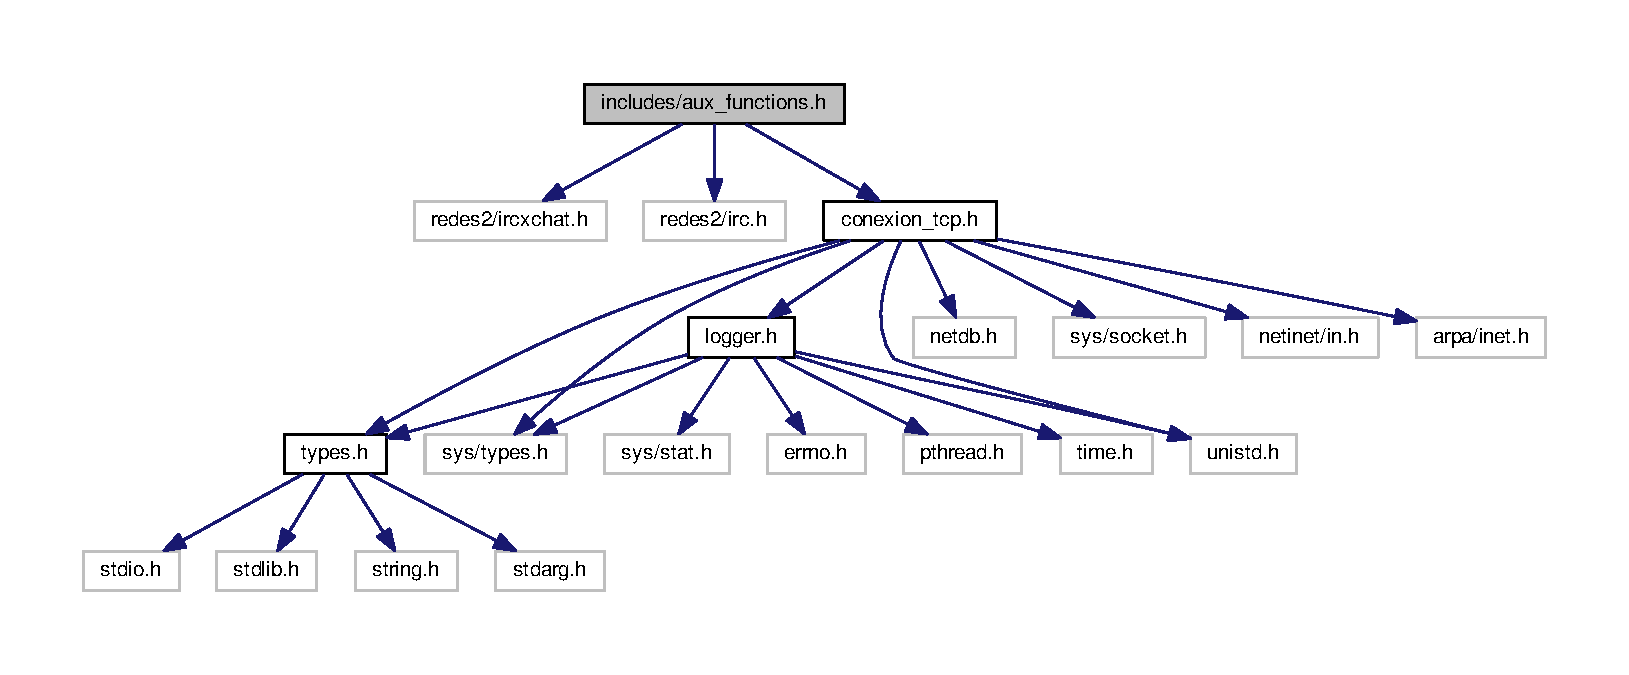
\includegraphics[width=350pt]{aux__functions_8h__incl}
\end{center}
\end{figure}
This graph shows which files directly or indirectly include this file\-:
\nopagebreak
\begin{figure}[H]
\begin{center}
\leavevmode
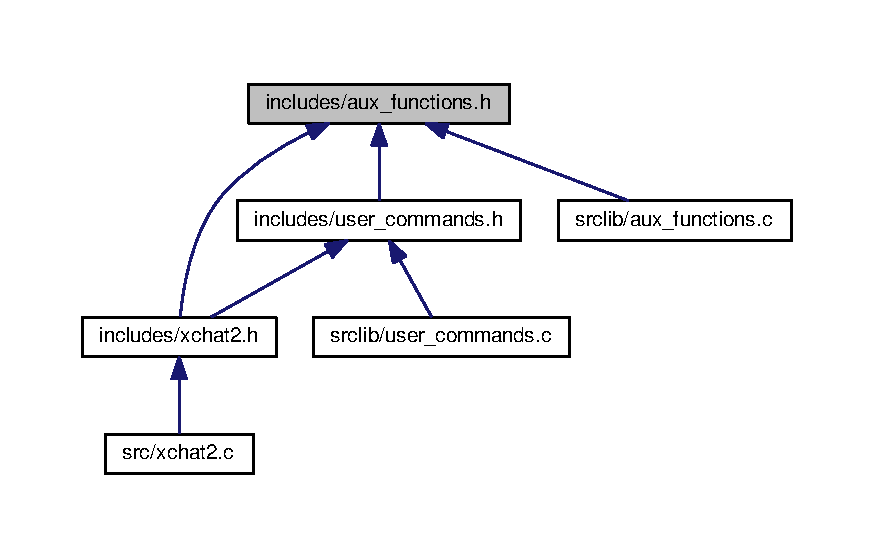
\includegraphics[width=350pt]{aux__functions_8h__dep__incl}
\end{center}
\end{figure}
\subsection*{Classes}
\begin{DoxyCompactItemize}
\item 
struct \hyperlink{struct_file__args}{File\-\_\-args}
\end{DoxyCompactItemize}
\subsection*{Macros}
\begin{DoxyCompactItemize}
\item 
\#define \hyperlink{aux__functions_8h_af4d98da13b92f926914c4a759759b393}{E\-X\-T\-R\-A}~20
\item 
\#define \hyperlink{aux__functions_8h_a9e8ece425678b8ada57d963482ca7c63}{S\-N\-A\-P\-\_\-\-S\-I\-Z\-E}~9
\item 
\#define \hyperlink{aux__functions_8h_a0eb099cedadf6c8aebb6b92b34d71631}{M\-A\-X\-\_\-\-N\-I\-C\-K\-\_\-\-F\-I\-E\-L\-D}~22+\hyperlink{aux__functions_8h_af4d98da13b92f926914c4a759759b393}{E\-X\-T\-R\-A}
\end{DoxyCompactItemize}
\subsection*{Functions}
\begin{DoxyCompactItemize}
\item 
void \hyperlink{aux__functions_8h_a2480cc4793bf25a16cc731dc9d033582}{mfree} (int n,...)
\begin{DoxyCompactList}\small\item\em Libera punteros si estos no estan a N\-U\-L\-L Uso. \end{DoxyCompactList}\item 
int \hyperlink{aux__functions_8h_a9a7f9a514711f5954007dc83533d9362}{save\-\_\-file} (void $\ast$args)
\begin{DoxyCompactList}\small\item\em Establece la conexíon con el servidor de archivos para recibir los datos y escribirlos en un fichero. \end{DoxyCompactList}\item 
void \hyperlink{aux__functions_8h_a09c2fcb81e148a2f23080a1671869f96}{interface\-\_\-mostrar\-\_\-nicks} (char $\ast$channel, char $\ast$list)
\begin{DoxyCompactList}\small\item\em Actualiza la lista de nicks de la interfaz y sus estados. \end{DoxyCompactList}\item 
char $\ast$ \hyperlink{aux__functions_8h_a20f32d171da437faef7716e4b6e667dd}{strnext} (char $\ast$haystack, int ch)
\begin{DoxyCompactList}\small\item\em Devuelve una cadena que empieza inmediatamente después de la cadena 'haystack' tras la primera aparición de 'ch'. \end{DoxyCompactList}\item 
int \hyperlink{aux__functions_8h_a90798d5fe15fdd743f8802b0f154b854}{parse\-\_\-type} (const char $\ast$message)
\begin{DoxyCompactList}\small\item\em Devuelve el tipo de comando (código 3 digitos) de un mensaje no reconocido por I\-R\-C\-\_\-\-Command\-Query() \end{DoxyCompactList}\item 
int \hyperlink{aux__functions_8h_a1738b19e427c47733b310cbe08431a56}{parse\-\_\-type2} (const char $\ast$message)
\begin{DoxyCompactList}\small\item\em Versión 2 de pruebas. Devuelve el tipo de comando (código 3 digitos) de un mensaje no reconocido por I\-R\-C\-\_\-\-Command\-Query() \end{DoxyCompactList}\item 
void \hyperlink{aux__functions_8h_a040868784608606fad914fea56fc65b8}{I\-R\-C\-Interface\-\_\-\-Write\-System\-\_\-\-Pretty} (char $\ast$nick, char $\ast$msg)
\item 
void \hyperlink{aux__functions_8h_a043ae6695458ae3a85dc9da43cf9b751}{I\-R\-C\-Interface\-\_\-\-Write\-System\-Thread\-\_\-\-Pretty} (char $\ast$nick, char $\ast$msg)
\item 
void \hyperlink{aux__functions_8h_a6400bb2b7979a2393f0e84b6646a24fe}{I\-R\-C\-Interface\-\_\-\-Write\-Channel\-Thread\-\_\-\-Pretty} (char $\ast$chan, char $\ast$nick, char $\ast$msg)
\item 
int \hyperlink{aux__functions_8h_a8d3c58618c3bb95d81a542251062d19e}{test\-I\-R\-C\-\_\-\-Command\-Query} (char $\ast$message)
\item 
int \hyperlink{aux__functions_8h_a06340d30a60b297a60b17841767fad85}{change\-Mode} (char $\ast$channel, char $\ast$nick, char $\ast$mode)
\end{DoxyCompactItemize}
\subsection*{Variables}
\begin{DoxyCompactItemize}
\item 
int \hyperlink{aux__functions_8h_acd63fb8dbd9439219e2db08dfc173aa0}{sockfd\-\_\-user}
\end{DoxyCompactItemize}


\subsection{Detailed Description}
Declaraciones de funciones, definición de tipos\-: implementación de funciones auxiliares de xchat2. \begin{DoxyAuthor}{Author}
Alfonso Sebares 

Beatriz de Pablo 

Celia Mateos 
\end{DoxyAuthor}
\begin{DoxyDate}{Date}
20/03/17 
\end{DoxyDate}


\subsection{Macro Definition Documentation}
\hypertarget{aux__functions_8h_af4d98da13b92f926914c4a759759b393}{\index{aux\-\_\-functions.\-h@{aux\-\_\-functions.\-h}!E\-X\-T\-R\-A@{E\-X\-T\-R\-A}}
\index{E\-X\-T\-R\-A@{E\-X\-T\-R\-A}!aux_functions.h@{aux\-\_\-functions.\-h}}
\subsubsection[{E\-X\-T\-R\-A}]{\setlength{\rightskip}{0pt plus 5cm}\#define E\-X\-T\-R\-A~20}}\label{aux__functions_8h_af4d98da13b92f926914c4a759759b393}
espacio extra para pruebas de formato \hypertarget{aux__functions_8h_a0eb099cedadf6c8aebb6b92b34d71631}{\index{aux\-\_\-functions.\-h@{aux\-\_\-functions.\-h}!M\-A\-X\-\_\-\-N\-I\-C\-K\-\_\-\-F\-I\-E\-L\-D@{M\-A\-X\-\_\-\-N\-I\-C\-K\-\_\-\-F\-I\-E\-L\-D}}
\index{M\-A\-X\-\_\-\-N\-I\-C\-K\-\_\-\-F\-I\-E\-L\-D@{M\-A\-X\-\_\-\-N\-I\-C\-K\-\_\-\-F\-I\-E\-L\-D}!aux_functions.h@{aux\-\_\-functions.\-h}}
\subsubsection[{M\-A\-X\-\_\-\-N\-I\-C\-K\-\_\-\-F\-I\-E\-L\-D}]{\setlength{\rightskip}{0pt plus 5cm}\#define M\-A\-X\-\_\-\-N\-I\-C\-K\-\_\-\-F\-I\-E\-L\-D~22+{\bf E\-X\-T\-R\-A}}}\label{aux__functions_8h_a0eb099cedadf6c8aebb6b92b34d71631}
maximo del campo 'nick' en el cliente\-: 11(\mbox{[}snap de tiempo\mbox{]}) + 2(espacio y \textbackslash{}0) + 9(nick I\-R\-C) \hypertarget{aux__functions_8h_a9e8ece425678b8ada57d963482ca7c63}{\index{aux\-\_\-functions.\-h@{aux\-\_\-functions.\-h}!S\-N\-A\-P\-\_\-\-S\-I\-Z\-E@{S\-N\-A\-P\-\_\-\-S\-I\-Z\-E}}
\index{S\-N\-A\-P\-\_\-\-S\-I\-Z\-E@{S\-N\-A\-P\-\_\-\-S\-I\-Z\-E}!aux_functions.h@{aux\-\_\-functions.\-h}}
\subsubsection[{S\-N\-A\-P\-\_\-\-S\-I\-Z\-E}]{\setlength{\rightskip}{0pt plus 5cm}\#define S\-N\-A\-P\-\_\-\-S\-I\-Z\-E~9}}\label{aux__functions_8h_a9e8ece425678b8ada57d963482ca7c63}
X\-X\-:\-X\-X\-:X\-X\textbackslash{}0 

\subsection{Function Documentation}
\hypertarget{aux__functions_8h_a06340d30a60b297a60b17841767fad85}{\index{aux\-\_\-functions.\-h@{aux\-\_\-functions.\-h}!change\-Mode@{change\-Mode}}
\index{change\-Mode@{change\-Mode}!aux_functions.h@{aux\-\_\-functions.\-h}}
\subsubsection[{change\-Mode}]{\setlength{\rightskip}{0pt plus 5cm}int change\-Mode (
\begin{DoxyParamCaption}
\item[{char $\ast$}]{channel, }
\item[{char $\ast$}]{nick, }
\item[{char $\ast$}]{mode}
\end{DoxyParamCaption}
)}}\label{aux__functions_8h_a06340d30a60b297a60b17841767fad85}

\begin{DoxyCode}
334                                                      \{
335         \textcolor{keywordtype}{int} ret = -1;
336         \textcolor{keywordtype}{char} *command = NULL;
337 
338         \textcolor{comment}{//long IRCMsg\_Mode (char **command, char *prefix, char * channeloruser, char *mode, char *user)}
339         ret = IRCMsg\_Mode (&command, NULL, channel, mode, nick);
340         \textcolor{keywordflow}{if}(ret != IRC\_OK)\{
341                 g\_print(\hyperlink{types_8h_a8d23feea868a983c8c2b661e1e16972f}{RED} \textcolor{stringliteral}{"ERROR - In changeMode: Error en IRCMsg\_Mode, no devolvió IRC\_OK\(\backslash\)n"} 
      \hyperlink{types_8h_ab702106cf3b3e96750b6845ded4e0299}{RESET});
342                 \textcolor{keywordflow}{return} \hyperlink{types_8h_a735563036dced0b7d6cc98f97ea4978b}{ERR};
343         \}
344         ret = \hyperlink{conexion__tcp_8h_ab9468ce1338cfca5736ab407ba155f55}{enviarDatos}(\hyperlink{aux__functions_8h_acd63fb8dbd9439219e2db08dfc173aa0}{sockfd\_user}, command, strlen(command));
345         \textcolor{keywordflow}{if}(ret == \hyperlink{types_8h_a735563036dced0b7d6cc98f97ea4978b}{ERR})\{
346                 g\_print(\hyperlink{types_8h_a8d23feea868a983c8c2b661e1e16972f}{RED} \textcolor{stringliteral}{"ERROR - In changeMode: Error en enviarDatos, devolvió ERR\(\backslash\)n"} 
      \hyperlink{types_8h_ab702106cf3b3e96750b6845ded4e0299}{RESET});
347                 \textcolor{keywordflow}{return} \hyperlink{types_8h_a735563036dced0b7d6cc98f97ea4978b}{ERR};
348         \}
349         IRCInterface\_PlaneRegisterOutMessage(command);
350         free(command);
351 
352         \textcolor{keywordflow}{return} \hyperlink{daemon_8h_aba51915c87d64af47fb1cc59348961c9}{OK};
353 \}
\end{DoxyCode}


Here is the call graph for this function\-:
\nopagebreak
\begin{figure}[H]
\begin{center}
\leavevmode
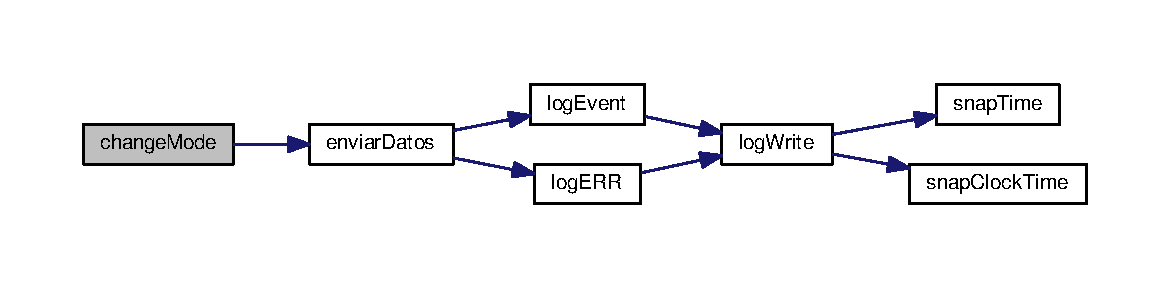
\includegraphics[width=350pt]{aux__functions_8h_a06340d30a60b297a60b17841767fad85_cgraph}
\end{center}
\end{figure}


\hypertarget{aux__functions_8h_a09c2fcb81e148a2f23080a1671869f96}{\index{aux\-\_\-functions.\-h@{aux\-\_\-functions.\-h}!interface\-\_\-mostrar\-\_\-nicks@{interface\-\_\-mostrar\-\_\-nicks}}
\index{interface\-\_\-mostrar\-\_\-nicks@{interface\-\_\-mostrar\-\_\-nicks}!aux_functions.h@{aux\-\_\-functions.\-h}}
\subsubsection[{interface\-\_\-mostrar\-\_\-nicks}]{\setlength{\rightskip}{0pt plus 5cm}void interface\-\_\-mostrar\-\_\-nicks (
\begin{DoxyParamCaption}
\item[{char $\ast$}]{channel, }
\item[{char $\ast$}]{list}
\end{DoxyParamCaption}
)}}\label{aux__functions_8h_a09c2fcb81e148a2f23080a1671869f96}


Actualiza la lista de nicks de la interfaz y sus estados. 


\begin{DoxyParams}{Parameters}
{\em channel} & canal que se quiere actualizar \\
\hline
{\em list} & lista de nicks obtenida del comando names, separados por espacios \\
\hline
\end{DoxyParams}
\begin{DoxyReturn}{Returns}
void 
\end{DoxyReturn}

\begin{DoxyCode}
161                                                        \{
162         g\_print(\hyperlink{types_8h_add9307de87f38e77d336751e305886f6}{BLU} \textcolor{stringliteral}{"\(\backslash\)n aux call: interface\_mostrar\_nicks() \(\backslash\)n"} \hyperlink{types_8h_ab702106cf3b3e96750b6845ded4e0299}{RESET});
163         \textcolor{keywordtype}{char}* show\_nick;
164         \textcolor{comment}{//obtenemos los nicks del mensaje y los mostramos por separado}
165 
166         \textcolor{comment}{//Eliminar los nicks del canal}
167         IRCInterface\_NickListChannelThread(channel, NULL, NULL, NULL, NULL, NONE, 0);
168 
169         show\_nick = strtok(list, \textcolor{stringliteral}{" "});
170         g\_print(\textcolor{stringliteral}{"channel: %s \(\backslash\)n"},channel);
171         g\_print(\textcolor{stringliteral}{"show\_nick: %s \(\backslash\)n"},show\_nick);
172         g\_print(\textcolor{stringliteral}{"list: %s \(\backslash\)n\(\backslash\)n"},list);
173         \textcolor{keywordflow}{if} (show\_nick[0] == \textcolor{charliteral}{'@'})
174         \{
175                 IRCInterface\_AddNickChannelThread (channel, ++show\_nick, list, list, list, OPERATOR);
176         \}\textcolor{keywordflow}{else} \textcolor{keywordflow}{if} (show\_nick[0] == \textcolor{charliteral}{'+'})\{
177                 IRCInterface\_AddNickChannelThread (channel, ++show\_nick, list, list, list, VOICE);
178         \} \textcolor{keywordflow}{else}\{
179                 IRCInterface\_AddNickChannelThread (channel, show\_nick, list, list, list, NONE);
180         \}
181         
182         \textcolor{keywordflow}{while} ((show\_nick = strtok(NULL, \textcolor{stringliteral}{" "})) != NULL)\{
183                 \textcolor{keywordflow}{if} (show\_nick[0] == \textcolor{charliteral}{'@'})
184                 \{
185                         IRCInterface\_AddNickChannelThread (channel, ++show\_nick, list, list, list, OPERATOR
      );
186                 \}\textcolor{keywordflow}{else} \textcolor{keywordflow}{if} (show\_nick[0] == \textcolor{charliteral}{'+'})\{
187                         IRCInterface\_AddNickChannelThread (channel, ++show\_nick, list, list, list, VOICE);
188                 \} \textcolor{keywordflow}{else}\{
189                         IRCInterface\_AddNickChannelThread (channel, show\_nick, list, list, list, NONE);
190                 \}
191         \}
192 \}
\end{DoxyCode}
\hypertarget{aux__functions_8h_a6400bb2b7979a2393f0e84b6646a24fe}{\index{aux\-\_\-functions.\-h@{aux\-\_\-functions.\-h}!I\-R\-C\-Interface\-\_\-\-Write\-Channel\-Thread\-\_\-\-Pretty@{I\-R\-C\-Interface\-\_\-\-Write\-Channel\-Thread\-\_\-\-Pretty}}
\index{I\-R\-C\-Interface\-\_\-\-Write\-Channel\-Thread\-\_\-\-Pretty@{I\-R\-C\-Interface\-\_\-\-Write\-Channel\-Thread\-\_\-\-Pretty}!aux_functions.h@{aux\-\_\-functions.\-h}}
\subsubsection[{I\-R\-C\-Interface\-\_\-\-Write\-Channel\-Thread\-\_\-\-Pretty}]{\setlength{\rightskip}{0pt plus 5cm}void I\-R\-C\-Interface\-\_\-\-Write\-Channel\-Thread\-\_\-\-Pretty (
\begin{DoxyParamCaption}
\item[{char $\ast$}]{chan, }
\item[{char $\ast$}]{nick, }
\item[{char $\ast$}]{msg}
\end{DoxyParamCaption}
)}}\label{aux__functions_8h_a6400bb2b7979a2393f0e84b6646a24fe}

\begin{DoxyCode}
306                                                                               \{
307         \textcolor{keywordtype}{char} snap[\hyperlink{aux__functions_8h_a9e8ece425678b8ada57d963482ca7c63}{SNAP\_SIZE}];
308         \textcolor{keywordtype}{char} f\_nick[\hyperlink{aux__functions_8h_a0eb099cedadf6c8aebb6b92b34d71631}{MAX\_NICK\_FIELD}];
309 
310         \textcolor{keywordflow}{if}(strlen(nick) > 9)\{
311                 \hyperlink{logger_8h_a9487660b2ec318326782a9d9e32f8461}{logERR}(\textcolor{stringliteral}{"En IRCInterface\_WriteSystemThread\_Pretty: strlen(nick) > 9"});
312                 \textcolor{keywordflow}{return};
313         \}
314 
315         strcpy(f\_nick, \textcolor{stringliteral}{"["});
316         strcat(f\_nick, \hyperlink{logger_8h_a9780074b15cc3acc70e3ee5989c8005a}{snapTime}(snap,\hyperlink{aux__functions_8h_a9e8ece425678b8ada57d963482ca7c63}{SNAP\_SIZE}));
317         strcat(f\_nick, \textcolor{stringliteral}{"]"});
318         strcat(f\_nick, nick);
319 
320         IRCInterface\_WriteChannelThread(chan, f\_nick, msg);     
321 \}
\end{DoxyCode}


Here is the call graph for this function\-:
\nopagebreak
\begin{figure}[H]
\begin{center}
\leavevmode
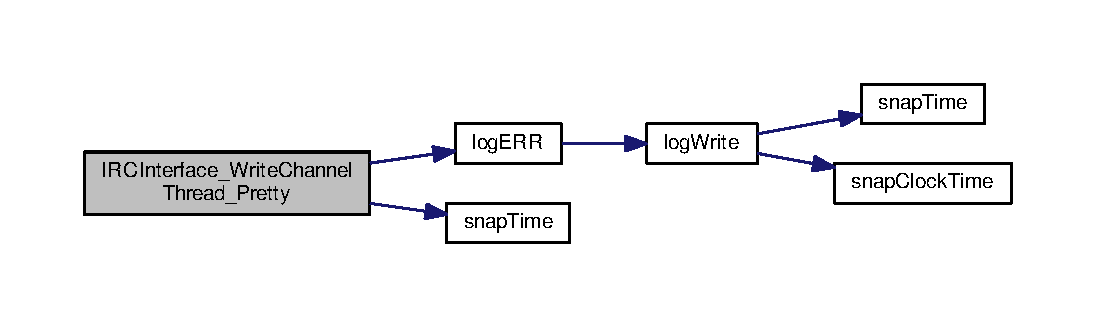
\includegraphics[width=350pt]{aux__functions_8h_a6400bb2b7979a2393f0e84b6646a24fe_cgraph}
\end{center}
\end{figure}


\hypertarget{aux__functions_8h_a040868784608606fad914fea56fc65b8}{\index{aux\-\_\-functions.\-h@{aux\-\_\-functions.\-h}!I\-R\-C\-Interface\-\_\-\-Write\-System\-\_\-\-Pretty@{I\-R\-C\-Interface\-\_\-\-Write\-System\-\_\-\-Pretty}}
\index{I\-R\-C\-Interface\-\_\-\-Write\-System\-\_\-\-Pretty@{I\-R\-C\-Interface\-\_\-\-Write\-System\-\_\-\-Pretty}!aux_functions.h@{aux\-\_\-functions.\-h}}
\subsubsection[{I\-R\-C\-Interface\-\_\-\-Write\-System\-\_\-\-Pretty}]{\setlength{\rightskip}{0pt plus 5cm}void I\-R\-C\-Interface\-\_\-\-Write\-System\-\_\-\-Pretty (
\begin{DoxyParamCaption}
\item[{char $\ast$}]{nick, }
\item[{char $\ast$}]{msg}
\end{DoxyParamCaption}
)}}\label{aux__functions_8h_a040868784608606fad914fea56fc65b8}

\begin{DoxyCode}
264                                                            \{
265         \textcolor{keywordtype}{char} snap[\hyperlink{aux__functions_8h_a9e8ece425678b8ada57d963482ca7c63}{SNAP\_SIZE}];
266         \textcolor{keywordtype}{char} f\_nick[\hyperlink{aux__functions_8h_a0eb099cedadf6c8aebb6b92b34d71631}{MAX\_NICK\_FIELD}];
267 
268         \textcolor{keywordflow}{if}(strlen(nick) > 9)\{
269                 \hyperlink{logger_8h_a9487660b2ec318326782a9d9e32f8461}{logERR}(\textcolor{stringliteral}{"En IRCInterface\_WriteSystemThread\_Pretty: strlen(nick) > 9"});
270                 \textcolor{keywordflow}{return};
271         \}
272 
273         strcpy(f\_nick, \textcolor{stringliteral}{"["});
274         strcat(f\_nick, \hyperlink{logger_8h_a9780074b15cc3acc70e3ee5989c8005a}{snapTime}(snap,\hyperlink{aux__functions_8h_a9e8ece425678b8ada57d963482ca7c63}{SNAP\_SIZE}));
275         strcat(f\_nick, \textcolor{stringliteral}{"] "});
276         strcat(f\_nick, \textcolor{stringliteral}{"              *"});
277 
278         \textcolor{comment}{//g\_print(MAG"\(\backslash\)n>>>>%s\(\backslash\)n" RESET, f\_nick);}
279         \textcolor{keywordflow}{if}(msg[strlen(msg) - 2] == 13) \textcolor{comment}{//check si es comienzo de CR,LF}
280                 msg[strlen(msg) - 2] = \textcolor{charliteral}{'\(\backslash\)0'};
281 
282         IRCInterface\_WriteSystem(f\_nick,msg);
283 \}
\end{DoxyCode}


Here is the call graph for this function\-:
\nopagebreak
\begin{figure}[H]
\begin{center}
\leavevmode
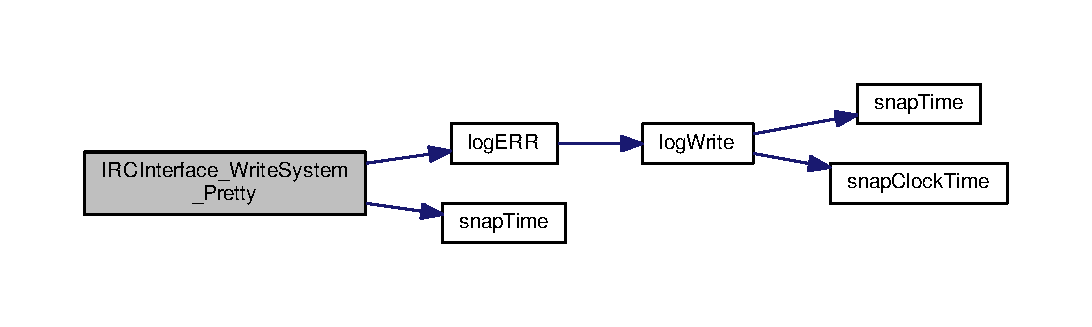
\includegraphics[width=350pt]{aux__functions_8h_a040868784608606fad914fea56fc65b8_cgraph}
\end{center}
\end{figure}


\hypertarget{aux__functions_8h_a043ae6695458ae3a85dc9da43cf9b751}{\index{aux\-\_\-functions.\-h@{aux\-\_\-functions.\-h}!I\-R\-C\-Interface\-\_\-\-Write\-System\-Thread\-\_\-\-Pretty@{I\-R\-C\-Interface\-\_\-\-Write\-System\-Thread\-\_\-\-Pretty}}
\index{I\-R\-C\-Interface\-\_\-\-Write\-System\-Thread\-\_\-\-Pretty@{I\-R\-C\-Interface\-\_\-\-Write\-System\-Thread\-\_\-\-Pretty}!aux_functions.h@{aux\-\_\-functions.\-h}}
\subsubsection[{I\-R\-C\-Interface\-\_\-\-Write\-System\-Thread\-\_\-\-Pretty}]{\setlength{\rightskip}{0pt plus 5cm}void I\-R\-C\-Interface\-\_\-\-Write\-System\-Thread\-\_\-\-Pretty (
\begin{DoxyParamCaption}
\item[{char $\ast$}]{nick, }
\item[{char $\ast$}]{msg}
\end{DoxyParamCaption}
)}}\label{aux__functions_8h_a043ae6695458ae3a85dc9da43cf9b751}

\begin{DoxyCode}
285                                                                  \{
286         \textcolor{keywordtype}{char} snap[\hyperlink{aux__functions_8h_a9e8ece425678b8ada57d963482ca7c63}{SNAP\_SIZE}];
287         \textcolor{keywordtype}{char} f\_nick[\hyperlink{aux__functions_8h_a0eb099cedadf6c8aebb6b92b34d71631}{MAX\_NICK\_FIELD}];
288 
289         \textcolor{keywordflow}{if}(strlen(nick) > 9)\{
290                 \hyperlink{logger_8h_a9487660b2ec318326782a9d9e32f8461}{logERR}(\textcolor{stringliteral}{"En IRCInterface\_WriteSystemThread\_Pretty: strlen(nick) > 9"});
291                 \textcolor{keywordflow}{return};
292         \}
293 
294         strcpy(f\_nick, \textcolor{stringliteral}{"["});
295         strcat(f\_nick, \hyperlink{logger_8h_a9780074b15cc3acc70e3ee5989c8005a}{snapTime}(snap,\hyperlink{aux__functions_8h_a9e8ece425678b8ada57d963482ca7c63}{SNAP\_SIZE}));
296         strcat(f\_nick, \textcolor{stringliteral}{"] "});
297         strcat(f\_nick, \textcolor{stringliteral}{"              *"});
298 
299         \textcolor{comment}{//g\_print(MAG"\(\backslash\)n>>>>%s\(\backslash\)n" RESET, f\_nick);}
300         \textcolor{keywordflow}{if}(msg[strlen(msg) - 2] == 13) \textcolor{comment}{//check si es comienzo de CR,LF}
301                 msg[strlen(msg) - 2] = \textcolor{charliteral}{'\(\backslash\)0'};
302 
303         IRCInterface\_WriteSystemThread(f\_nick,msg);
304 \}
\end{DoxyCode}


Here is the call graph for this function\-:
\nopagebreak
\begin{figure}[H]
\begin{center}
\leavevmode
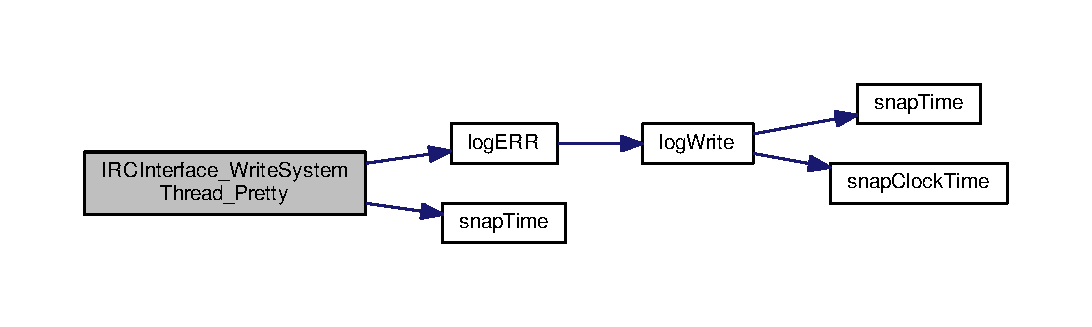
\includegraphics[width=350pt]{aux__functions_8h_a043ae6695458ae3a85dc9da43cf9b751_cgraph}
\end{center}
\end{figure}


\hypertarget{aux__functions_8h_a2480cc4793bf25a16cc731dc9d033582}{\index{aux\-\_\-functions.\-h@{aux\-\_\-functions.\-h}!mfree@{mfree}}
\index{mfree@{mfree}!aux_functions.h@{aux\-\_\-functions.\-h}}
\subsubsection[{mfree}]{\setlength{\rightskip}{0pt plus 5cm}void mfree (
\begin{DoxyParamCaption}
\item[{int}]{n, }
\item[{}]{...}
\end{DoxyParamCaption}
)}}\label{aux__functions_8h_a2480cc4793bf25a16cc731dc9d033582}


Libera punteros si estos no estan a N\-U\-L\-L Uso. 

mfree(3,a,b,c); mfree(4,a,b,c,d); 
\begin{DoxyCode}
20                       \{
21 
22         va\_list ap;
23         \textcolor{keywordtype}{char} *p = NULL;
24         \textcolor{keyword}{register} \textcolor{keywordtype}{int} i;
25         va\_start(ap, n);
26         \textcolor{keywordflow}{for} (i = 0; i < n; ++i)
27         \{
28                 p = (\textcolor{keywordtype}{char} *) va\_arg(ap, \textcolor{keywordtype}{char}*);
29                 \textcolor{keywordflow}{if}( p != NULL) free(p);
30         \}
31         va\_end (ap);
32 \}
\end{DoxyCode}
\hypertarget{aux__functions_8h_a90798d5fe15fdd743f8802b0f154b854}{\index{aux\-\_\-functions.\-h@{aux\-\_\-functions.\-h}!parse\-\_\-type@{parse\-\_\-type}}
\index{parse\-\_\-type@{parse\-\_\-type}!aux_functions.h@{aux\-\_\-functions.\-h}}
\subsubsection[{parse\-\_\-type}]{\setlength{\rightskip}{0pt plus 5cm}int parse\-\_\-type (
\begin{DoxyParamCaption}
\item[{const char $\ast$}]{message}
\end{DoxyParamCaption}
)}}\label{aux__functions_8h_a90798d5fe15fdd743f8802b0f154b854}


Devuelve el tipo de comando (código 3 digitos) de un mensaje no reconocido por I\-R\-C\-\_\-\-Command\-Query() 


\begin{DoxyParams}{Parameters}
{\em message} & mensaje original \\
\hline
\end{DoxyParams}
\begin{DoxyReturn}{Returns}
int codigo de comando si es un codigo valido, E\-R\-R si no lo es o comando invalido 
\end{DoxyReturn}

\begin{DoxyCode}
219                                    \{
220         \textcolor{keywordtype}{int} unknw\_type;
221         \textcolor{keywordtype}{char}* token = NULL;
222         \textcolor{keywordtype}{char}* message\_cp = NULL;
223 
224         \textcolor{keywordflow}{if}(message[0] == \textcolor{charliteral}{':'})\{ \textcolor{comment}{//mensaje con prefijo, no originado por el cliente}
225                 message\_cp = strdup(message);
226                 token = strtok(message\_cp, \textcolor{stringliteral}{" "});
227                 \textcolor{keywordflow}{if}(token != NULL)\{
228                         token = strtok(NULL, \textcolor{stringliteral}{" "});
229                         free(message\_cp);
230                         unknw\_type = atoi(token);
231                         \textcolor{keywordflow}{if} (unknw\_type < \hyperlink{types_8h_a8756b6216508f7f2f20ebc934889ee77}{MAX\_IRC\_COMMAND})\{
232                                 \textcolor{keywordflow}{return} unknw\_type;
233                         \}
234                 \}
235         \}
236 
237         \textcolor{keywordflow}{return} \hyperlink{types_8h_a735563036dced0b7d6cc98f97ea4978b}{ERR};
238 \}
\end{DoxyCode}
\hypertarget{aux__functions_8h_a1738b19e427c47733b310cbe08431a56}{\index{aux\-\_\-functions.\-h@{aux\-\_\-functions.\-h}!parse\-\_\-type2@{parse\-\_\-type2}}
\index{parse\-\_\-type2@{parse\-\_\-type2}!aux_functions.h@{aux\-\_\-functions.\-h}}
\subsubsection[{parse\-\_\-type2}]{\setlength{\rightskip}{0pt plus 5cm}int parse\-\_\-type2 (
\begin{DoxyParamCaption}
\item[{const char $\ast$}]{message}
\end{DoxyParamCaption}
)}}\label{aux__functions_8h_a1738b19e427c47733b310cbe08431a56}


Versión 2 de pruebas. Devuelve el tipo de comando (código 3 digitos) de un mensaje no reconocido por I\-R\-C\-\_\-\-Command\-Query() 


\begin{DoxyParams}{Parameters}
{\em message} & mensaje original \\
\hline
\end{DoxyParams}
\begin{DoxyReturn}{Returns}
int codigo de comando si es un codigo valido, E\-R\-R si no lo es o comando invalido 
\end{DoxyReturn}

\begin{DoxyCode}
245                                     \{
246         \textcolor{keywordtype}{int} unknw\_type;
247         \textcolor{keywordtype}{char}* token = NULL;
248         \textcolor{keywordtype}{char}* message\_cp = NULL;
249 
250         message\_cp = strdup(message);
251         token = strtok(message\_cp, \textcolor{stringliteral}{" "});
252         \textcolor{keywordflow}{if}(token != NULL)\{
253                 token = strtok(NULL, \textcolor{stringliteral}{" "});
254                 free(message\_cp);
255                 unknw\_type = atoi(token);
256                 \textcolor{keywordflow}{if} (unknw\_type < \hyperlink{types_8h_a8756b6216508f7f2f20ebc934889ee77}{MAX\_IRC\_COMMAND})\{
257                         \textcolor{keywordflow}{return} unknw\_type;
258                 \}
259         \}
260         
261         \textcolor{keywordflow}{return} \hyperlink{types_8h_a735563036dced0b7d6cc98f97ea4978b}{ERR};
262 \}
\end{DoxyCode}
\hypertarget{aux__functions_8h_a9a7f9a514711f5954007dc83533d9362}{\index{aux\-\_\-functions.\-h@{aux\-\_\-functions.\-h}!save\-\_\-file@{save\-\_\-file}}
\index{save\-\_\-file@{save\-\_\-file}!aux_functions.h@{aux\-\_\-functions.\-h}}
\subsubsection[{save\-\_\-file}]{\setlength{\rightskip}{0pt plus 5cm}int save\-\_\-file (
\begin{DoxyParamCaption}
\item[{void $\ast$}]{args}
\end{DoxyParamCaption}
)}}\label{aux__functions_8h_a9a7f9a514711f5954007dc83533d9362}


Establece la conexíon con el servidor de archivos para recibir los datos y escribirlos en un fichero. 


\begin{DoxyParams}{Parameters}
{\em args} & estructura que contiene los parametros necesarios para establacer la conexion \\
\hline
\end{DoxyParams}
\begin{DoxyReturn}{Returns}
O\-K si todo fue correcto y E\-R\-R si ocurrio un error 
\end{DoxyReturn}

\begin{DoxyCode}
39                          \{
40 
41         g\_print(\textcolor{stringliteral}{"\(\backslash\)n =========save\_file========= \(\backslash\)n"});
42 
43         \hyperlink{struct_file__args}{File\_args}* file\_args = (\hyperlink{struct_file__args}{File\_args}*) args;
44         FILE* file = fopen(file\_args->\hyperlink{struct_file__args_ad24dfcb255f29ee677793a0051c7336b}{filename},\textcolor{stringliteral}{"w"});
45         \textcolor{keywordtype}{char} message[\hyperlink{types_8h_ae7e715c270481406658bbd2bafa2897f}{MAXDATA}];
46         g\_print(\textcolor{stringliteral}{"Guardamos el archivo\(\backslash\)n"});
47 
48         \textcolor{keyword}{struct }hostent *he;
49     \textcolor{keyword}{struct }in\_addr **addr\_list;
50     \textcolor{keywordtype}{int} i=0;
51     \textcolor{keywordtype}{char} ip\_addr[INET\_ADDRSTRLEN]=\textcolor{stringliteral}{""};
52     sleep(2);
53     g\_print(\textcolor{stringliteral}{"file\_args->hostname: %s \(\backslash\)nfile\_args->port: %d \(\backslash\)n"},file\_args->
      \hyperlink{struct_file__args_a9aa177aea3a099397a09131a92f30115}{hostname}, file\_args->\hyperlink{struct_file__args_a83e78eb2ebacdc7e63eca61d1340fa61}{port}); 
54 
55     \textcolor{keywordtype}{int} file\_sockfd;
56 
57     \textcolor{keywordflow}{if} ((he = gethostbyname(file\_args->\hyperlink{struct_file__args_a9aa177aea3a099397a09131a92f30115}{hostname})) == NULL) \{  \textcolor{comment}{// get the host info}
58         g\_print(\textcolor{stringliteral}{"ERROR: IRCInterface\_Connect - gethostbyname\(\backslash\)n"});
59         \textcolor{keywordflow}{return} \hyperlink{types_8h_a735563036dced0b7d6cc98f97ea4978b}{ERR};
60     \}
61 
62     \textcolor{comment}{// print information about this host:}
63     g\_print(\textcolor{stringliteral}{"Official name is: %s\(\backslash\)n"}, he->h\_name);
64     g\_print(\textcolor{stringliteral}{"    IP addresses: "});
65     addr\_list = (\textcolor{keyword}{struct }in\_addr **)he->h\_addr\_list;
66     \textcolor{keywordflow}{for}(i = 0; addr\_list[i] != NULL; i++) \{
67         strcat(ip\_addr,inet\_ntoa(*addr\_list[i]));
68         g\_print(\textcolor{stringliteral}{"%s "}, inet\_ntoa(*addr\_list[i]));
69     \}
70     g\_print(\textcolor{stringliteral}{"\(\backslash\)n"});
71     g\_print(\textcolor{stringliteral}{"ip\_addr: %s \(\backslash\)n"},ip\_addr); 
72 
73     \textcolor{keyword}{struct }sockaddr\_in server\_struct;
74     memset(&server\_struct, \textcolor{charliteral}{'0'}, \textcolor{keyword}{sizeof}(server\_struct)); 
75     server\_struct.sin\_family = AF\_INET;
76     server\_struct.sin\_port = htons(file\_args->\hyperlink{struct_file__args_a83e78eb2ebacdc7e63eca61d1340fa61}{port});
77         \textcolor{comment}{//server\_struct.sin\_port = file\_args->port;}
78     \textcolor{comment}{//memset(&(server\_struct.sin\_zero), '\(\backslash\)0', 8);}
79     server\_struct.sin\_addr = **addr\_list;
80 
81     \textcolor{comment}{//Socket}
82     file\_sockfd = socket(AF\_INET,SOCK\_STREAM,0);
83     \textcolor{keywordflow}{if} (file\_sockfd == -1)\{
84         g\_print(\textcolor{stringliteral}{"Error creando socket\(\backslash\)n"});
85         \textcolor{keywordflow}{return} \hyperlink{types_8h_a735563036dced0b7d6cc98f97ea4978b}{ERR};
86     \}
87     \textcolor{comment}{//Connect}
88     g\_print(\textcolor{stringliteral}{"Conectando con socket %d\(\backslash\)n"},file\_sockfd);
89     \textcolor{keywordtype}{int} cnct = connect(file\_sockfd, (\textcolor{keyword}{struct} sockaddr*)&server\_struct, \textcolor{keyword}{sizeof}(server\_struct));
90         \textcolor{keywordflow}{if} (cnct==-1)\{
91                         \textcolor{keywordflow}{switch}(errno)\{
92                                 \textcolor{keywordflow}{case} EACCES:
93                                 printf(\textcolor{stringliteral}{"For UNIX domain sockets, which are identified by pathname: Write
       permission is denied on the socket file, or search permission is denied for one of the directories in the path
       prefix. (See also path\_resolution(7).) \(\backslash\)n"});
94                                         printf(\textcolor{stringliteral}{"or The user tried to connect to a broadcast address without
       having the socket broadcast flag enabled or the connection request failed because of a local firewall rule.
      \(\backslash\)n"} );
95                                                                         
96                                         \textcolor{keywordflow}{break};
97                                 
98                                 \textcolor{keywordflow}{case} EPERM:
99                                         printf(\textcolor{stringliteral}{"The user tried to connect to a broadcast address without
       having the socket broadcast flag enabled or the connection request failed because of a local firewall rule.\(\backslash\)n"}
      ); 
100                                         \textcolor{keywordflow}{break};
101                                 \textcolor{keywordflow}{case} EADDRINUSE:
102                                 printf(\textcolor{stringliteral}{"Local address is already in use. \(\backslash\)n"});
103                                         \textcolor{keywordflow}{break};
104                                 \textcolor{keywordflow}{case} EAFNOSUPPORT:
105                                 printf(\textcolor{stringliteral}{"The passed address didn't have the correct address family in its
       sa\_family field. \(\backslash\)n"});
106                                         \textcolor{keywordflow}{break};
107                                 \textcolor{keywordflow}{case} EAGAIN:
108                                     printf(\textcolor{stringliteral}{"No more free local ports or insufficient entries in the routing
       cache. For AF\_INET see the description of /proc/sys/net/ipv4/ip\_local\_port\_range ip(7) for information on
       how to increase the number of local ports. \(\backslash\)n"});
109                                         \textcolor{keywordflow}{break};
110                                 \textcolor{keywordflow}{case} EALREADY:
111                                     printf(\textcolor{stringliteral}{"The socket is nonblocking and a previous connection attempt has
       not yet been completed.\(\backslash\)n"}); 
112                                         \textcolor{keywordflow}{break};
113                                 \textcolor{keywordflow}{case} EBADF:
114                                     printf(\textcolor{stringliteral}{"The file descriptor is not a valid index in the descriptor
       table.\(\backslash\)n"}); 
115                                         \textcolor{keywordflow}{break};
116                                 \textcolor{keywordflow}{case} ECONNREFUSED:
117                                     printf(\textcolor{stringliteral}{"No-one listening on the remote address. \(\backslash\)n"});
118                                         \textcolor{keywordflow}{break};
119                                 \textcolor{keywordflow}{case} EFAULT:
120                                     printf(\textcolor{stringliteral}{"The socket structure address is outside the user's address
       space. \(\backslash\)n"});
121                                         \textcolor{keywordflow}{break};
122                                 \textcolor{keywordflow}{case} EINPROGRESS:
123                                     printf(\textcolor{stringliteral}{"The socket is nonblocking and the connection cannot be
       completed immediately. It is possible to select(2) or poll(2) for completion by selecting the socket for writing.
       After select(2) indicates writability, use getsockopt(2) to read the SO\_ERROR option at level SOL\_SOCKET to
       determine whether connect() completed successfully (SO\_ERROR is zero) or unsuccessfully (SO\_ERROR is one of
       the usual error codes listed here, explaining the reason for the failure). \(\backslash\)n"}); 
124                                         \textcolor{keywordflow}{break};
125                                 \textcolor{keywordflow}{case} EINTR:
126                                     printf(\textcolor{stringliteral}{"The system call was interrupted by a signal that was caught;
       see signal(7).\(\backslash\)n"}); 
127                                         \textcolor{keywordflow}{break};
128                                 \textcolor{keywordflow}{case} EISCONN:
129                                     printf(\textcolor{stringliteral}{"The socket is already connected.\(\backslash\)n"}); 
130                                         \textcolor{keywordflow}{break};
131                                 \textcolor{keywordflow}{case} ENETUNREACH:
132                                     printf(\textcolor{stringliteral}{"Network is unreachable. \(\backslash\)n"});
133                                         \textcolor{keywordflow}{break};
134                                 \textcolor{keywordflow}{case} ENOTSOCK:
135                                     printf(\textcolor{stringliteral}{"The file descriptor is not associated with a socket.\(\backslash\)n"}); 
136                                         \textcolor{keywordflow}{break};
137                                 \textcolor{keywordflow}{case} ETIMEDOUT:
138                                     printf(\textcolor{stringliteral}{"Timeout while attempting connection. The server may be too busy
       to accept new connections. Note that for IP sockets the timeout may be very long when syncookies are
       enabled on the server.\(\backslash\)n"});
139                                     \textcolor{keywordflow}{break};
140                         \}
141                 \textcolor{keywordflow}{return} -1;
142         \}
143 
144         g\_print(\textcolor{stringliteral}{"Campos recibidos: hostname=%s, filename=%s, port=%d, length=%ld\(\backslash\)n"},file\_args->
      \hyperlink{struct_file__args_a9aa177aea3a099397a09131a92f30115}{hostname}, file\_args->\hyperlink{struct_file__args_ad24dfcb255f29ee677793a0051c7336b}{filename}, file\_args->\hyperlink{struct_file__args_a83e78eb2ebacdc7e63eca61d1340fa61}{port}, file\_args->
      \hyperlink{struct_file__args_a3168e8734e7ad263d88a6da49b4aff20}{length});
145         
146         \hyperlink{conexion__tcp_8h_a2ec2b47883bdb05804bec657bfc42516}{recvDatos}(file\_sockfd, message, \hyperlink{types_8h_ae7e715c270481406658bbd2bafa2897f}{MAXDATA}, he->h\_name);
147         g\_print(\textcolor{stringliteral}{"Estoy recibiendo datos\(\backslash\)n"});
148         fputs(message, file);
149         \textcolor{comment}{//fwrite(message, 1, sizeof(message), file);}
150         g\_print(\textcolor{stringliteral}{"Algo paso...\(\backslash\)n"});
151 
152         \textcolor{keywordflow}{return} \hyperlink{daemon_8h_aba51915c87d64af47fb1cc59348961c9}{OK};
153 \}
\end{DoxyCode}


Here is the call graph for this function\-:
\nopagebreak
\begin{figure}[H]
\begin{center}
\leavevmode
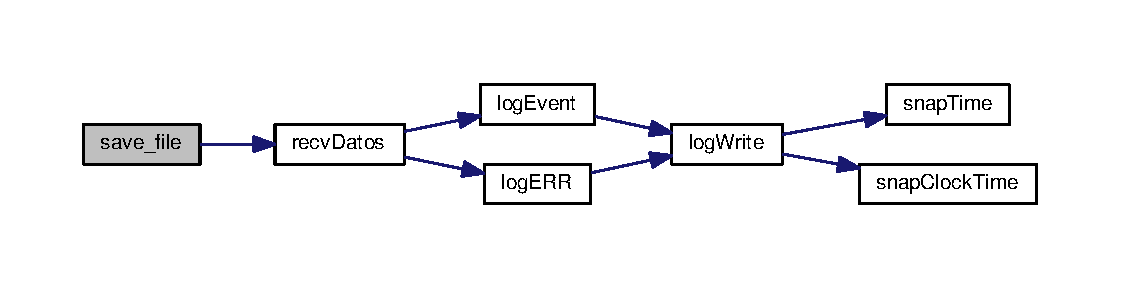
\includegraphics[width=350pt]{aux__functions_8h_a9a7f9a514711f5954007dc83533d9362_cgraph}
\end{center}
\end{figure}


\hypertarget{aux__functions_8h_a20f32d171da437faef7716e4b6e667dd}{\index{aux\-\_\-functions.\-h@{aux\-\_\-functions.\-h}!strnext@{strnext}}
\index{strnext@{strnext}!aux_functions.h@{aux\-\_\-functions.\-h}}
\subsubsection[{strnext}]{\setlength{\rightskip}{0pt plus 5cm}char$\ast$ strnext (
\begin{DoxyParamCaption}
\item[{char $\ast$}]{haystack, }
\item[{int}]{ch}
\end{DoxyParamCaption}
)}}\label{aux__functions_8h_a20f32d171da437faef7716e4b6e667dd}


Devuelve una cadena que empieza inmediatamente después de la cadena 'haystack' tras la primera aparición de 'ch'. 


\begin{DoxyParams}{Parameters}
{\em haystack} & string original donde hacer la busqueda \\
\hline
{\em ch} & delimitador \\
\hline
\end{DoxyParams}
\begin{DoxyReturn}{Returns}
char$\ast$ substring con la cadena generada, N\-U\-L\-L si no se ha encontrado 'ch' 
\end{DoxyReturn}

\begin{DoxyCode}
200                                      \{
201         \textcolor{keywordtype}{int} i, o\_length;
202         \textcolor{keywordtype}{char} *sep\_at = strchr(haystack, ch);
203         
204         \textcolor{keywordflow}{if}(sep\_at != NULL)\{
205                 o\_length = strlen(sep\_at);
206                 \textcolor{keywordflow}{for}(i=0; i<strlen(sep\_at); i++)
207                         sep\_at[i] = sep\_at[i+1];
208                 sep\_at[o\_length-1] = \textcolor{charliteral}{'\(\backslash\)0'};
209         \}
210 
211         \textcolor{keywordflow}{return} sep\_at;
212 \}
\end{DoxyCode}
\hypertarget{aux__functions_8h_a8d3c58618c3bb95d81a542251062d19e}{\index{aux\-\_\-functions.\-h@{aux\-\_\-functions.\-h}!test\-I\-R\-C\-\_\-\-Command\-Query@{test\-I\-R\-C\-\_\-\-Command\-Query}}
\index{test\-I\-R\-C\-\_\-\-Command\-Query@{test\-I\-R\-C\-\_\-\-Command\-Query}!aux_functions.h@{aux\-\_\-functions.\-h}}
\subsubsection[{test\-I\-R\-C\-\_\-\-Command\-Query}]{\setlength{\rightskip}{0pt plus 5cm}int test\-I\-R\-C\-\_\-\-Command\-Query (
\begin{DoxyParamCaption}
\item[{char $\ast$}]{message}
\end{DoxyParamCaption}
)}}\label{aux__functions_8h_a8d3c58618c3bb95d81a542251062d19e}

\begin{DoxyCode}
323                                        \{
324         \textcolor{keywordflow}{switch}(IRC\_CommandQuery(message))\{
325                 \textcolor{keywordflow}{case} IRCERR\_NOCOMMAND:
326                         \textcolor{keywordflow}{return} \hyperlink{types_8h_a735563036dced0b7d6cc98f97ea4978b}{ERR};
327                 \textcolor{keywordflow}{case} IRCERR\_UNKNOWNCOMMAND:
328                         \textcolor{keywordflow}{return} \hyperlink{types_8h_a735563036dced0b7d6cc98f97ea4978b}{ERR};
329                 \textcolor{keywordflow}{default}:
330                         \textcolor{keywordflow}{return} \hyperlink{daemon_8h_aba51915c87d64af47fb1cc59348961c9}{OK};
331         \}
332 \}
\end{DoxyCode}


\subsection{Variable Documentation}
\hypertarget{aux__functions_8h_acd63fb8dbd9439219e2db08dfc173aa0}{\index{aux\-\_\-functions.\-h@{aux\-\_\-functions.\-h}!sockfd\-\_\-user@{sockfd\-\_\-user}}
\index{sockfd\-\_\-user@{sockfd\-\_\-user}!aux_functions.h@{aux\-\_\-functions.\-h}}
\subsubsection[{sockfd\-\_\-user}]{\setlength{\rightskip}{0pt plus 5cm}int sockfd\-\_\-user}}\label{aux__functions_8h_acd63fb8dbd9439219e2db08dfc173aa0}
global con el socket que tiene abierto el cliente con el servidor I\-R\-C

descriptor con el socket abierto con el servidor 
\hypertarget{conexion__tcp_8h}{\section{includes/conexion\-\_\-tcp.h File Reference}
\label{conexion__tcp_8h}\index{includes/conexion\-\_\-tcp.\-h@{includes/conexion\-\_\-tcp.\-h}}
}


Declaraciones de funciones, definición de tipos\-: liberia para conexiones T\-C\-P.  


{\ttfamily \#include \char`\"{}types.\-h\char`\"{}}\\*
{\ttfamily \#include \char`\"{}logger.\-h\char`\"{}}\\*
{\ttfamily \#include $<$unistd.\-h$>$}\\*
{\ttfamily \#include $<$netdb.\-h$>$}\\*
{\ttfamily \#include $<$sys/types.\-h$>$}\\*
{\ttfamily \#include $<$sys/socket.\-h$>$}\\*
{\ttfamily \#include $<$netinet/in.\-h$>$}\\*
{\ttfamily \#include $<$arpa/inet.\-h$>$}\\*
Include dependency graph for conexion\-\_\-tcp.\-h\-:
\nopagebreak
\begin{figure}[H]
\begin{center}
\leavevmode
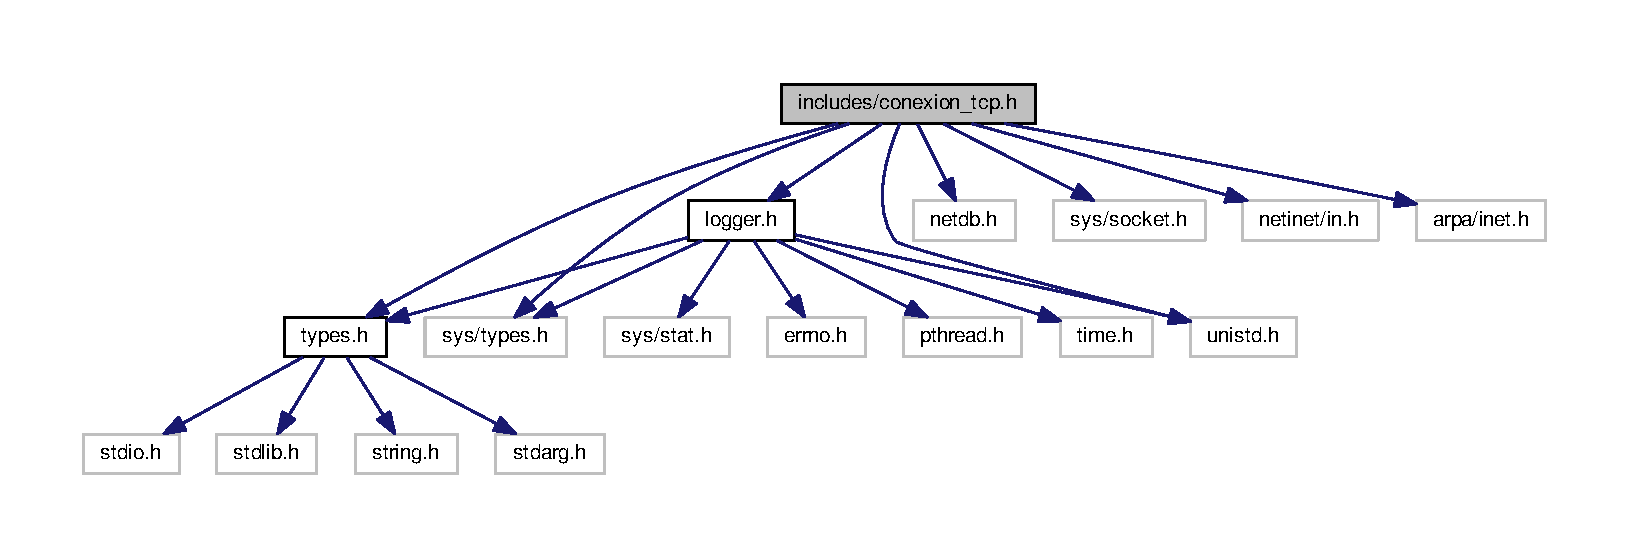
\includegraphics[width=350pt]{conexion__tcp_8h__incl}
\end{center}
\end{figure}
This graph shows which files directly or indirectly include this file\-:
\nopagebreak
\begin{figure}[H]
\begin{center}
\leavevmode
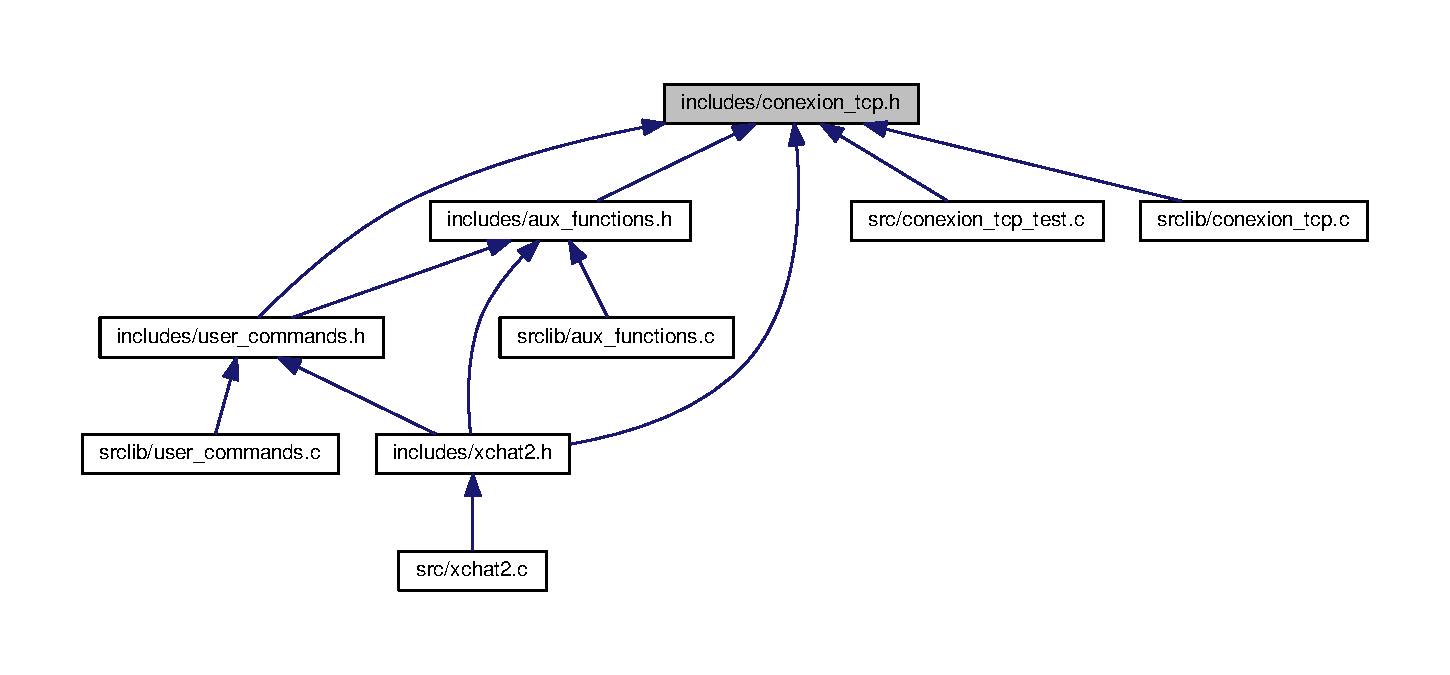
\includegraphics[width=350pt]{conexion__tcp_8h__dep__incl}
\end{center}
\end{figure}
\subsection*{Macros}
\begin{DoxyCompactItemize}
\item 
\#define \hyperlink{conexion__tcp_8h_aeca034f67218340ecb2261a22c2f3dcd}{B\-U\-F\-S\-I\-Z\-E}~1024
\item 
\#define \hyperlink{conexion__tcp_8h_a6c224620c83dd3234d005fd90eb82207}{A\-U\-X\-\_\-\-S\-B\-U\-F}~1152
\item 
\#define \hyperlink{conexion__tcp_8h_a3e4b4faa36cc9e3a7d9895aec8f27592}{M\-A\-X\-\_\-\-C\-O\-N\-\_\-\-R\-E\-Q}~10
\end{DoxyCompactItemize}
\subsection*{Functions}
\begin{DoxyCompactItemize}
\item 
int \hyperlink{conexion__tcp_8h_a7180696e651a403677ea6a35b59da285}{crear\-Conexion} (int portno, struct sockaddr\-\_\-in $\ast$server)
\item 
int \hyperlink{conexion__tcp_8h_a2ec2b47883bdb05804bec657bfc42516}{recv\-Datos} (int client\-\_\-sock, char $\ast$client\-\_\-message, int cm\-\_\-size, char $\ast$hostaddrp)
\item 
int \hyperlink{conexion__tcp_8h_ab9468ce1338cfca5736ab407ba155f55}{enviar\-Datos} (int client\-\_\-sock, char $\ast$message, int message\-\_\-size)
\item 
int \hyperlink{conexion__tcp_8h_a831321f466f7f9fa60b0f940b7c2d7da}{cerrar\-Conexion} (int client\-\_\-sock, char $\ast$hostaddrp)
\end{DoxyCompactItemize}


\subsection{Detailed Description}
Declaraciones de funciones, definición de tipos\-: liberia para conexiones T\-C\-P. \begin{DoxyAuthor}{Author}
Alfonso Sebares 

Beatriz de Pablo 

Celia Mateos 
\end{DoxyAuthor}
\begin{DoxyDate}{Date}
13/02/17 
\end{DoxyDate}


\subsection{Macro Definition Documentation}
\hypertarget{conexion__tcp_8h_a6c224620c83dd3234d005fd90eb82207}{\index{conexion\-\_\-tcp.\-h@{conexion\-\_\-tcp.\-h}!A\-U\-X\-\_\-\-S\-B\-U\-F@{A\-U\-X\-\_\-\-S\-B\-U\-F}}
\index{A\-U\-X\-\_\-\-S\-B\-U\-F@{A\-U\-X\-\_\-\-S\-B\-U\-F}!conexion_tcp.h@{conexion\-\_\-tcp.\-h}}
\subsubsection[{A\-U\-X\-\_\-\-S\-B\-U\-F}]{\setlength{\rightskip}{0pt plus 5cm}\#define A\-U\-X\-\_\-\-S\-B\-U\-F~1152}}\label{conexion__tcp_8h_a6c224620c83dd3234d005fd90eb82207}
Tam. max. del buffer auxiliar para logeo de eventos (1024 + 128 extra) \hypertarget{conexion__tcp_8h_aeca034f67218340ecb2261a22c2f3dcd}{\index{conexion\-\_\-tcp.\-h@{conexion\-\_\-tcp.\-h}!B\-U\-F\-S\-I\-Z\-E@{B\-U\-F\-S\-I\-Z\-E}}
\index{B\-U\-F\-S\-I\-Z\-E@{B\-U\-F\-S\-I\-Z\-E}!conexion_tcp.h@{conexion\-\_\-tcp.\-h}}
\subsubsection[{B\-U\-F\-S\-I\-Z\-E}]{\setlength{\rightskip}{0pt plus 5cm}\#define B\-U\-F\-S\-I\-Z\-E~1024}}\label{conexion__tcp_8h_aeca034f67218340ecb2261a22c2f3dcd}
Tam. max. del buffer que se lee \hypertarget{conexion__tcp_8h_a3e4b4faa36cc9e3a7d9895aec8f27592}{\index{conexion\-\_\-tcp.\-h@{conexion\-\_\-tcp.\-h}!M\-A\-X\-\_\-\-C\-O\-N\-\_\-\-R\-E\-Q@{M\-A\-X\-\_\-\-C\-O\-N\-\_\-\-R\-E\-Q}}
\index{M\-A\-X\-\_\-\-C\-O\-N\-\_\-\-R\-E\-Q@{M\-A\-X\-\_\-\-C\-O\-N\-\_\-\-R\-E\-Q}!conexion_tcp.h@{conexion\-\_\-tcp.\-h}}
\subsubsection[{M\-A\-X\-\_\-\-C\-O\-N\-\_\-\-R\-E\-Q}]{\setlength{\rightskip}{0pt plus 5cm}\#define M\-A\-X\-\_\-\-C\-O\-N\-\_\-\-R\-E\-Q~10}}\label{conexion__tcp_8h_a3e4b4faa36cc9e3a7d9895aec8f27592}
Max. de peticiones de conexion activas (e.\-g. la 11 falla si puesto a 10) 

\subsection{Function Documentation}
\hypertarget{conexion__tcp_8h_a831321f466f7f9fa60b0f940b7c2d7da}{\index{conexion\-\_\-tcp.\-h@{conexion\-\_\-tcp.\-h}!cerrar\-Conexion@{cerrar\-Conexion}}
\index{cerrar\-Conexion@{cerrar\-Conexion}!conexion_tcp.h@{conexion\-\_\-tcp.\-h}}
\subsubsection[{cerrar\-Conexion}]{\setlength{\rightskip}{0pt plus 5cm}int cerrar\-Conexion (
\begin{DoxyParamCaption}
\item[{int}]{client\-\_\-sock, }
\item[{char $\ast$}]{hostaddrp}
\end{DoxyParamCaption}
)}}\label{conexion__tcp_8h_a831321f466f7f9fa60b0f940b7c2d7da}

\begin{DoxyCode}
113                                                     \{
114         \textcolor{keywordtype}{int} sent\_size;
115         \textcolor{keywordtype}{char} buf[\hyperlink{conexion__tcp_8h_a6c224620c83dd3234d005fd90eb82207}{AUX\_SBUF}];
116 
117         \textcolor{keywordflow}{if}(close(client\_sock) < 0)\{
118         \hyperlink{logger_8h_a9487660b2ec318326782a9d9e32f8461}{logERR}(\textcolor{stringliteral}{"Error al cerrar la conexion"});
119         \textcolor{keywordflow}{return} \hyperlink{types_8h_a735563036dced0b7d6cc98f97ea4978b}{ERR};
120 
121     \}\textcolor{keywordflow}{else}\{
122         \textcolor{keywordflow}{if} (hostaddrp != NULL)
123                         sprintf(buf, \textcolor{stringliteral}{"conexion\_tcp.c: conexion cerrada con %s"}, hostaddrp);
124                 \textcolor{keywordflow}{else}
125                         sprintf(buf, \textcolor{stringliteral}{"conexion\_tcp.c: conexion cerrada"});
126                 \hyperlink{logger_8h_af71188329ee1cf68a59d3f9ddd035ca6}{logEvent}(buf);
127     \}
128 
129     \textcolor{keywordflow}{return} \hyperlink{daemon_8h_aba51915c87d64af47fb1cc59348961c9}{OK};
130 \}\end{DoxyCode}


Here is the call graph for this function\-:
\nopagebreak
\begin{figure}[H]
\begin{center}
\leavevmode
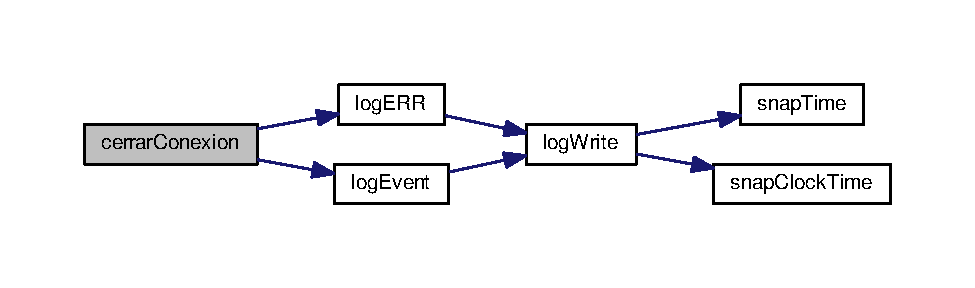
\includegraphics[width=350pt]{conexion__tcp_8h_a831321f466f7f9fa60b0f940b7c2d7da_cgraph}
\end{center}
\end{figure}


\hypertarget{conexion__tcp_8h_a7180696e651a403677ea6a35b59da285}{\index{conexion\-\_\-tcp.\-h@{conexion\-\_\-tcp.\-h}!crear\-Conexion@{crear\-Conexion}}
\index{crear\-Conexion@{crear\-Conexion}!conexion_tcp.h@{conexion\-\_\-tcp.\-h}}
\subsubsection[{crear\-Conexion}]{\setlength{\rightskip}{0pt plus 5cm}int crear\-Conexion (
\begin{DoxyParamCaption}
\item[{int}]{portno, }
\item[{struct sockaddr\-\_\-in $\ast$}]{server}
\end{DoxyParamCaption}
)}}\label{conexion__tcp_8h_a7180696e651a403677ea6a35b59da285}

\begin{DoxyCode}
15                                                          \{
16         \textcolor{keywordtype}{int} socket\_desc;
17         \textcolor{keywordtype}{int} optval;                                             \textcolor{comment}{/* flag value for setsockopt */}
18         
19         \textcolor{comment}{//Create socket}
20         socket\_desc = socket(AF\_INET , SOCK\_STREAM , 0);
21         \textcolor{keywordflow}{if} (socket\_desc == -1)
22         \{
23                 \hyperlink{logger_8h_a9487660b2ec318326782a9d9e32f8461}{logERR}(\textcolor{stringliteral}{"No se ha podido crear socket"});
24                 \textcolor{keywordflow}{return} \hyperlink{types_8h_a735563036dced0b7d6cc98f97ea4978b}{ERR};
25         \}
26 
27         \hyperlink{logger_8h_af71188329ee1cf68a59d3f9ddd035ca6}{logEvent}(\textcolor{stringliteral}{"Socket creado"});
28         
29         optval = 1;
30 
31         setsockopt(socket\_desc, SOL\_SOCKET, SO\_REUSEADDR, (\textcolor{keyword}{const} \textcolor{keywordtype}{void} *)&optval , \textcolor{keyword}{sizeof}(\textcolor{keywordtype}{int}));
32 
33         \textcolor{comment}{//Prepare the sockaddr\_in structure}
34         memset((\textcolor{keywordtype}{char} *) server, 0, \textcolor{keyword}{sizeof}(*server));
35         server->sin\_family = AF\_INET;
36         server->sin\_addr.s\_addr = INADDR\_ANY;
37         server->sin\_port = htons((\textcolor{keywordtype}{unsigned} \textcolor{keywordtype}{short})portno );
38          
39         \textcolor{comment}{//Bind}
40         \textcolor{keywordflow}{if}( bind(socket\_desc,(\textcolor{keyword}{struct} sockaddr *)server , \textcolor{keyword}{sizeof}(*server)) < 0)
41         \{
42                 \hyperlink{logger_8h_a9487660b2ec318326782a9d9e32f8461}{logERR}(\textcolor{stringliteral}{"bind failed"});
43                 \textcolor{keywordflow}{return} \hyperlink{types_8h_a735563036dced0b7d6cc98f97ea4978b}{ERR};
44         \}
45         \hyperlink{logger_8h_af71188329ee1cf68a59d3f9ddd035ca6}{logEvent}(\textcolor{stringliteral}{"bind done"});
46          
47         \textcolor{comment}{//Listen}
48         listen(socket\_desc , \hyperlink{conexion__tcp_8h_a3e4b4faa36cc9e3a7d9895aec8f27592}{MAX\_CON\_REQ});
49          
50         \textcolor{comment}{//Accept and incoming connection}
51         \hyperlink{logger_8h_af71188329ee1cf68a59d3f9ddd035ca6}{logEvent}(\textcolor{stringliteral}{"Esperando conexiones entrantes..."});
52         
53         \textcolor{keywordflow}{return} socket\_desc;
54 \}
\end{DoxyCode}


Here is the call graph for this function\-:
\nopagebreak
\begin{figure}[H]
\begin{center}
\leavevmode
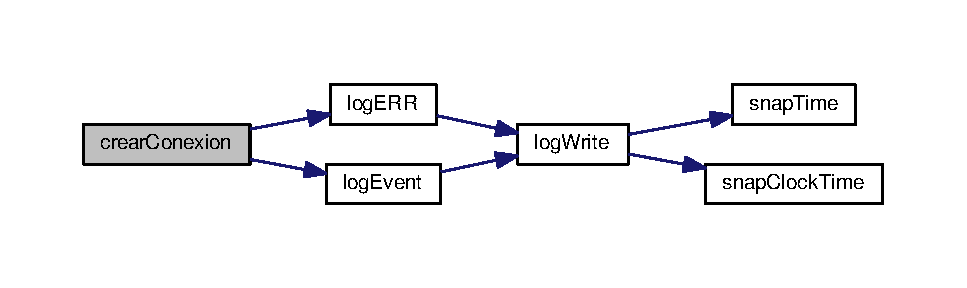
\includegraphics[width=350pt]{conexion__tcp_8h_a7180696e651a403677ea6a35b59da285_cgraph}
\end{center}
\end{figure}


\hypertarget{conexion__tcp_8h_ab9468ce1338cfca5736ab407ba155f55}{\index{conexion\-\_\-tcp.\-h@{conexion\-\_\-tcp.\-h}!enviar\-Datos@{enviar\-Datos}}
\index{enviar\-Datos@{enviar\-Datos}!conexion_tcp.h@{conexion\-\_\-tcp.\-h}}
\subsubsection[{enviar\-Datos}]{\setlength{\rightskip}{0pt plus 5cm}int enviar\-Datos (
\begin{DoxyParamCaption}
\item[{int}]{client\-\_\-sock, }
\item[{char $\ast$}]{message, }
\item[{int}]{message\-\_\-size}
\end{DoxyParamCaption}
)}}\label{conexion__tcp_8h_ab9468ce1338cfca5736ab407ba155f55}

\begin{DoxyCode}
87                                                                  \{
88         \textcolor{keywordtype}{int} sent\_size;
89         \textcolor{keywordtype}{char} buf[\hyperlink{conexion__tcp_8h_a6c224620c83dd3234d005fd90eb82207}{AUX\_SBUF}];
90 
91         sent\_size = send(client\_sock, message, message\_size, 0);
92 
93         \textcolor{keywordflow}{if} (sent\_size == 0)\{
94         \hyperlink{logger_8h_af71188329ee1cf68a59d3f9ddd035ca6}{logEvent}(\textcolor{stringliteral}{"send(): enviado un tam 0 bytes"});
95                 \textcolor{keywordflow}{return} 0;
96 
97     \}\textcolor{keywordflow}{else} \textcolor{keywordflow}{if}(sent\_size < 0)\{
98                 \hyperlink{logger_8h_a9487660b2ec318326782a9d9e32f8461}{logERR}(\textcolor{stringliteral}{"send(): enviado un tam -1 bytes, error"});
99                 \textcolor{keywordflow}{return} \hyperlink{types_8h_a735563036dced0b7d6cc98f97ea4978b}{ERR};
100 
101         \}\textcolor{keywordflow}{else}\{
102                 \textcolor{comment}{//printf("\(\backslash\)nYEE '%d', '%d', '%d'\(\backslash\)n", message[strlen(message) - 3], message[strlen(message)
       - 2], message[strlen(message) - 1]);}
103                 \textcolor{comment}{//if(message[strlen(message) - 2] == 13) //check si es CR,LF}
104                 \textcolor{comment}{//      message[strlen(message) - 2] = '\(\backslash\)0';}
105                 sprintf(buf, \textcolor{stringliteral}{"send(): \(\backslash\)"%s\(\backslash\)" (%d Bytes)"}, message, sent\_size);
106                 \hyperlink{logger_8h_af71188329ee1cf68a59d3f9ddd035ca6}{logEvent}(buf);
107         \}
108 
109     \textcolor{keywordflow}{return} sent\_size;
110 \}
\end{DoxyCode}


Here is the call graph for this function\-:
\nopagebreak
\begin{figure}[H]
\begin{center}
\leavevmode
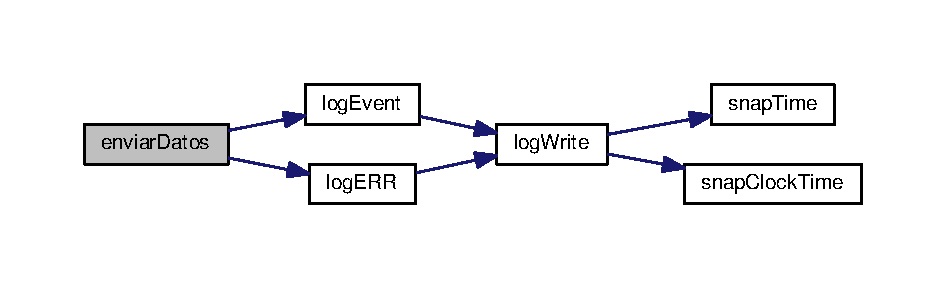
\includegraphics[width=350pt]{conexion__tcp_8h_ab9468ce1338cfca5736ab407ba155f55_cgraph}
\end{center}
\end{figure}


\hypertarget{conexion__tcp_8h_a2ec2b47883bdb05804bec657bfc42516}{\index{conexion\-\_\-tcp.\-h@{conexion\-\_\-tcp.\-h}!recv\-Datos@{recv\-Datos}}
\index{recv\-Datos@{recv\-Datos}!conexion_tcp.h@{conexion\-\_\-tcp.\-h}}
\subsubsection[{recv\-Datos}]{\setlength{\rightskip}{0pt plus 5cm}int recv\-Datos (
\begin{DoxyParamCaption}
\item[{int}]{client\-\_\-sock, }
\item[{char $\ast$}]{client\-\_\-message, }
\item[{int}]{cm\-\_\-size, }
\item[{char $\ast$}]{hostaddrp}
\end{DoxyParamCaption}
)}}\label{conexion__tcp_8h_a2ec2b47883bdb05804bec657bfc42516}

\begin{DoxyCode}
57                                                                                   \{
58         \textcolor{keywordtype}{int} read\_size;
59         \textcolor{keywordtype}{char} buf[\hyperlink{conexion__tcp_8h_a6c224620c83dd3234d005fd90eb82207}{AUX\_SBUF}];
60 
61         read\_size = recv(client\_sock , client\_message , cm\_size , 0);
62 
63         \textcolor{keywordflow}{if} (read\_size == 0)\{
64                 sprintf(buf,\textcolor{stringliteral}{"recv(): leido un tam 0 bytes de %s"}, hostaddrp);
65                 \hyperlink{logger_8h_af71188329ee1cf68a59d3f9ddd035ca6}{logEvent}(buf);
66                 \textcolor{keywordflow}{return} 0;
67 
68         \}\textcolor{keywordflow}{else} \textcolor{keywordflow}{if}(read\_size < 0)\{
69                 sprintf(buf,\textcolor{stringliteral}{"recv(): leido un tam -1 bytes de %s, error"}, hostaddrp);
70                 \hyperlink{logger_8h_a9487660b2ec318326782a9d9e32f8461}{logERR}(buf);
71                 \textcolor{keywordflow}{return} \hyperlink{types_8h_a735563036dced0b7d6cc98f97ea4978b}{ERR};
72 
73         \}\textcolor{keywordflow}{else}\{
74                 \textcolor{comment}{//if(client\_message[strlen(client\_message) - 2] == 13) //check si es CR,LF}
75                 \textcolor{comment}{//      client\_message[strlen(client\_message) - 2] = '\(\backslash\)0';}
76                 sprintf(buf, \textcolor{stringliteral}{"recv(): \(\backslash\)"%s\(\backslash\)" (%d Bytes) de %s"}, client\_message, read\_size, hostaddrp);
77                 \hyperlink{logger_8h_af71188329ee1cf68a59d3f9ddd035ca6}{logEvent}(buf);
78         \}
79 
80         \textcolor{keywordflow}{return} read\_size;
81 \}
\end{DoxyCode}


Here is the call graph for this function\-:
\nopagebreak
\begin{figure}[H]
\begin{center}
\leavevmode
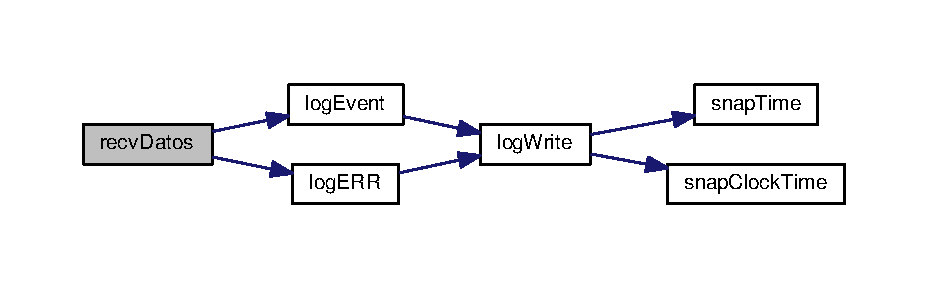
\includegraphics[width=350pt]{conexion__tcp_8h_a2ec2b47883bdb05804bec657bfc42516_cgraph}
\end{center}
\end{figure}



\hypertarget{daemon_8h}{}\section{includes/daemon.h File Reference}
\label{daemon_8h}\index{includes/daemon.\+h@{includes/daemon.\+h}}


Prototipo de funciones para daemonizar el servidor I\+RC.  


{\ttfamily \#include $<$redes2/irc.\+h$>$}\\*
{\ttfamily \#include $<$syslog.\+h$>$}\\*
{\ttfamily \#include $<$sys/stat.\+h$>$}\\*
Include dependency graph for daemon.\+h\+:
% FIG 0
This graph shows which files directly or indirectly include this file\+:
% FIG 1
\subsection*{Macros}
\begin{DoxyCompactItemize}
\item 
\#define \hyperlink{daemon_8h_aba51915c87d64af47fb1cc59348961c9}{OK}~0
\item 
\#define \hyperlink{daemon_8h_a8fe83ac76edc595f6b98cd4a4127aed5}{E\+R\+R\+OR}~-\/1
\end{DoxyCompactItemize}
\subsection*{Functions}
\begin{Indent}{\bf daemonizar}\par
{\em Funcion para demonizar a un servicio, crear proceso, unirlo al init e inhabilitar la terminal


\begin{DoxyParams}{Parameters}
{\em char} & $\ast$ servicio\+: Nombre del servidor para dejarlo en segundo plano\\
\hline
\end{DoxyParams}
\begin{DoxyReturn}{Returns}
OK si todo ha salido bien, E\+R\+R\+OR si hay algun fallo 
\end{DoxyReturn}
}\begin{DoxyCompactItemize}
\item 
int \hyperlink{daemon_8h_ae983f3eb0ff5cebb14c2ae123043df39}{daemonizar} (char $\ast$servicio)
\begin{DoxyCompactList}\small\item\em Funcion para demonizar a un servicio. \end{DoxyCompactList}\end{DoxyCompactItemize}
\end{Indent}


\subsection{Detailed Description}
Prototipo de funciones para daemonizar el servidor I\+RC. 

\begin{DoxyAuthor}{Author}
Alfonso Sebares 

Beatriz de Pablo 
\end{DoxyAuthor}


\subsection{Macro Definition Documentation}
\index{daemon.\+h@{daemon.\+h}!E\+R\+R\+OR@{E\+R\+R\+OR}}
\index{E\+R\+R\+OR@{E\+R\+R\+OR}!daemon.\+h@{daemon.\+h}}
\subsubsection[{\texorpdfstring{E\+R\+R\+OR}{ERROR}}]{\setlength{\rightskip}{0pt plus 5cm}\#define E\+R\+R\+OR~-\/1}\hypertarget{daemon_8h_a8fe83ac76edc595f6b98cd4a4127aed5}{}\label{daemon_8h_a8fe83ac76edc595f6b98cd4a4127aed5}
\index{daemon.\+h@{daemon.\+h}!OK@{OK}}
\index{OK@{OK}!daemon.\+h@{daemon.\+h}}
\subsubsection[{\texorpdfstring{OK}{OK}}]{\setlength{\rightskip}{0pt plus 5cm}\#define OK~0}\hypertarget{daemon_8h_aba51915c87d64af47fb1cc59348961c9}{}\label{daemon_8h_aba51915c87d64af47fb1cc59348961c9}


\subsection{Function Documentation}
\index{daemon.\+h@{daemon.\+h}!daemonizar@{daemonizar}}
\index{daemonizar@{daemonizar}!daemon.\+h@{daemon.\+h}}
\subsubsection[{\texorpdfstring{daemonizar(char $\ast$servicio)}{daemonizar(char *servicio)}}]{\setlength{\rightskip}{0pt plus 5cm}int daemonizar (
\begin{DoxyParamCaption}
\item[{char $\ast$}]{servicio}
\end{DoxyParamCaption}
)}\hypertarget{daemon_8h_ae983f3eb0ff5cebb14c2ae123043df39}{}\label{daemon_8h_ae983f3eb0ff5cebb14c2ae123043df39}


Funcion para demonizar a un servicio. 


\begin{DoxyParams}{Parameters}
{\em char} & $\ast$ servicio\+: Nombre del servidor para dejarlo en segundo plano \\
\hline
\end{DoxyParams}
\begin{DoxyReturn}{Returns}
OK si todo ha salido bien, E\+R\+R\+OR si hay algun fallo 
\end{DoxyReturn}

\begin{DoxyCode}
16                                  \{
17 
18         pid\_t pid;
19         pid\_t sid;
20 
21         \textcolor{keywordflow}{if} (servicio==NULL)\{
22                 syslog(LOG\_ERR, \textcolor{stringliteral}{"Escriba un servicio no nulo."});
23                 \textcolor{keywordflow}{return} \hyperlink{daemon_8h_a8fe83ac76edc595f6b98cd4a4127aed5}{ERROR};
24         \}
25 
26         \textcolor{comment}{/* 1. Ceamos proceso hijo y terminamos el proceso padre */}
27         pid=fork();
28 
29         \textcolor{keywordflow}{if} (pid < 0) \{
30                 syslog(LOG\_ERR, \textcolor{stringliteral}{"Error al crear proceso hijo"});
31                 \textcolor{keywordflow}{return} \hyperlink{daemon_8h_a8fe83ac76edc595f6b98cd4a4127aed5}{ERROR};
32         \}
33         \textcolor{keywordflow}{if} (pid > 0) \{
34                 syslog(LOG\_INFO, \textcolor{stringliteral}{"Liberando al padre"});
35                 \textcolor{keywordflow}{return} \hyperlink{daemon_8h_aba51915c87d64af47fb1cc59348961c9}{OK};
36         \}
37 
38         
39         \textcolor{comment}{/* 2. Crear una nueva sesión de tal forma que el proceso pase a ser lider de sesión, y no sea un
       zombie. */}
40         sid=setsid();
41         \textcolor{keywordflow}{if} (sid < 0) \{
42                 syslog (LOG\_ERR, \textcolor{stringliteral}{"Error creando un SID para el hijo del proceso"});
43                 \textcolor{keywordflow}{return} \hyperlink{daemon_8h_a8fe83ac76edc595f6b98cd4a4127aed5}{ERROR};
44         \}
45 
46         
47         \textcolor{comment}{/* 3. Cambiar la máscara para que los ficheros sean accesibles a cualquiera (0) */}
48         umask (0);
49 
50         \textcolor{comment}{/* 4. Establecer el directorio raíz / como directorio de trabajo */}
51         \textcolor{keywordflow}{if}((chdir(\textcolor{stringliteral}{"/"})) < 0)\{
52                 syslog (LOG\_ERR, \textcolor{stringliteral}{"Error al cambiar el directorio de trabajo a la raíz"});
53                 \textcolor{keywordflow}{return} \hyperlink{daemon_8h_a8fe83ac76edc595f6b98cd4a4127aed5}{ERROR};
54         \}
55 
56         \textcolor{comment}{/* 5. Cerrar todos los descriptores de fichero que pueda haber abiertos ya que no se puede usar la
       terminal*/}
57         syslog(LOG\_INFO, \textcolor{stringliteral}{"Cerrando descriptores"});
58 
59         close(STDIN\_FILENO); 
60         close(STDOUT\_FILENO);
61         close(STDERR\_FILENO);
62 
63         syslog(LOG\_INFO, \textcolor{stringliteral}{"Mandando descriptores a dev/null.."});
64         
65         freopen(\textcolor{stringliteral}{"/dev/null"}, \textcolor{stringliteral}{"r"}, stdin);
66         freopen(\textcolor{stringliteral}{"/dev/null"}, \textcolor{stringliteral}{"w"}, stdout);
67         freopen(\textcolor{stringliteral}{"/dev/null"}, \textcolor{stringliteral}{"w"}, stderr);
68 
69         \textcolor{comment}{/* 6. Abrir el log del sistema para su uso posterior (para que haya comunicacion con el demonio) */}
70         openlog (servicio, LOG\_CONS | LOG\_PID | LOG\_NDELAY, LOG\_LOCAL3);
71 
72         syslog (LOG\_INFO, \textcolor{stringliteral}{"Iniciado nuevo servidor"});
73 
74         \textcolor{keywordflow}{return} \hyperlink{daemon_8h_aba51915c87d64af47fb1cc59348961c9}{OK};
75 \}
\end{DoxyCode}

\hypertarget{logger_8h}{}\section{includes/logger.h File Reference}
\label{logger_8h}\index{includes/logger.\+h@{includes/logger.\+h}}
{\ttfamily \#include \char`\"{}types.\+h\char`\"{}}\\*
{\ttfamily \#include $<$time.\+h$>$}\\*
{\ttfamily \#include $<$sys/types.\+h$>$}\\*
{\ttfamily \#include $<$sys/stat.\+h$>$}\\*
{\ttfamily \#include $<$unistd.\+h$>$}\\*
{\ttfamily \#include $<$errno.\+h$>$}\\*
{\ttfamily \#include $<$pthread.\+h$>$}\\*
Include dependency graph for logger.\+h\+:
% FIG 0
This graph shows which files directly or indirectly include this file\+:
% FIG 1
\subsection*{Classes}
\begin{DoxyCompactItemize}
\item 
struct \hyperlink{structval}{val}
\end{DoxyCompactItemize}
\subsection*{Macros}
\begin{DoxyCompactItemize}
\item 
\#define \hyperlink{logger_8h_a05b49c662c073f89e86804f7856622a0}{L\+EN}~64
\item 
\#define \hyperlink{logger_8h_a3ed7c007f5ae003384ef18cb88f337ea}{B\+I\+G\+L\+EN}~1536
\end{DoxyCompactItemize}
\subsection*{Typedefs}
\begin{DoxyCompactItemize}
\item 
typedef struct \hyperlink{structval}{val} \hyperlink{logger_8h_a99ac4d25315947f8928b8239c69c8173}{val\+\_\+struct}
\end{DoxyCompactItemize}
\subsection*{Functions}
\begin{DoxyCompactItemize}
\item 
char $\ast$ \hyperlink{logger_8h_a9780074b15cc3acc70e3ee5989c8005a}{snap\+Time} (char $\ast$buf, int len)
\item 
char $\ast$ \hyperlink{logger_8h_ad5ed54850fd750ca0935368e72017537}{snap\+Clock\+Time} (char $\ast$buf, int len)
\item 
F\+I\+LE $\ast$ \hyperlink{logger_8h_a1fa2e9d39664def63d53e3d576dc923f}{init\+Log} ()
\item 
int \hyperlink{logger_8h_a6d1f5cd19f49b187e2097a467eca0233}{log\+Write} (char $\ast$log\+\_\+msg, char $\ast$type)
\item 
int \hyperlink{logger_8h_af71188329ee1cf68a59d3f9ddd035ca6}{log\+Event} (char $\ast$log\+\_\+msg)
\item 
int \hyperlink{logger_8h_a9487660b2ec318326782a9d9e32f8461}{log\+E\+RR} (char $\ast$log\+\_\+msg)
\end{DoxyCompactItemize}
\subsection*{Variables}
\begin{DoxyCompactItemize}
\item 
pthread\+\_\+mutex\+\_\+t \hyperlink{logger_8h_a53497b00bd1ff0270ca7a108d5794dbc}{loglock}
\begin{DoxyCompactList}\small\item\em Declaracion del Mutex para el descriptor de fichero del log. Siempre tiene que ser definida en el source princpal. \end{DoxyCompactList}\end{DoxyCompactItemize}


\subsection{Macro Definition Documentation}
\index{logger.\+h@{logger.\+h}!B\+I\+G\+L\+EN@{B\+I\+G\+L\+EN}}
\index{B\+I\+G\+L\+EN@{B\+I\+G\+L\+EN}!logger.\+h@{logger.\+h}}
\subsubsection[{\texorpdfstring{B\+I\+G\+L\+EN}{BIGLEN}}]{\setlength{\rightskip}{0pt plus 5cm}\#define B\+I\+G\+L\+EN~1536}\hypertarget{logger_8h_a3ed7c007f5ae003384ef18cb88f337ea}{}\label{logger_8h_a3ed7c007f5ae003384ef18cb88f337ea}
tam de buffer para mensajes grabados en .log (1024 + 512, orientativo) \index{logger.\+h@{logger.\+h}!L\+EN@{L\+EN}}
\index{L\+EN@{L\+EN}!logger.\+h@{logger.\+h}}
\subsubsection[{\texorpdfstring{L\+EN}{LEN}}]{\setlength{\rightskip}{0pt plus 5cm}\#define L\+EN~64}\hypertarget{logger_8h_a05b49c662c073f89e86804f7856622a0}{}\label{logger_8h_a05b49c662c073f89e86804f7856622a0}
tam de buffer para snaps de tiempo 

\subsection{Typedef Documentation}
\index{logger.\+h@{logger.\+h}!val\+\_\+struct@{val\+\_\+struct}}
\index{val\+\_\+struct@{val\+\_\+struct}!logger.\+h@{logger.\+h}}
\subsubsection[{\texorpdfstring{val\+\_\+struct}{val_struct}}]{\setlength{\rightskip}{0pt plus 5cm}typedef struct {\bf val} {\bf val\+\_\+struct}}\hypertarget{logger_8h_a99ac4d25315947f8928b8239c69c8173}{}\label{logger_8h_a99ac4d25315947f8928b8239c69c8173}


\subsection{Function Documentation}
\index{logger.\+h@{logger.\+h}!init\+Log@{init\+Log}}
\index{init\+Log@{init\+Log}!logger.\+h@{logger.\+h}}
\subsubsection[{\texorpdfstring{init\+Log()}{initLog()}}]{\setlength{\rightskip}{0pt plus 5cm}F\+I\+LE$\ast$ init\+Log (
\begin{DoxyParamCaption}
{}
\end{DoxyParamCaption}
)}\hypertarget{logger_8h_a1fa2e9d39664def63d53e3d576dc923f}{}\label{logger_8h_a1fa2e9d39664def63d53e3d576dc923f}

\begin{DoxyCode}
37                \{
38         \textcolor{keywordtype}{char} buf[\hyperlink{logger_8h_a05b49c662c073f89e86804f7856622a0}{LEN}];
39         \textcolor{keywordtype}{char} log\_dir[\hyperlink{logger_8h_a05b49c662c073f89e86804f7856622a0}{LEN}];
40         \textcolor{keyword}{struct }stat st = \{0\};
41         \textcolor{keywordtype}{int} ret = 0;
42         FILE *fp = NULL;
43 
44         \textcolor{keywordflow}{if} (stat(\textcolor{stringliteral}{"logs"}, &st) == -1) \{
45                 \textcolor{comment}{//ret = mkdir("logs", 0700);}
46                 \textcolor{keywordflow}{if} ( (ret = mkdir(\textcolor{stringliteral}{"logs"}, ACCESSPERMS)) != \hyperlink{daemon_8h_aba51915c87d64af47fb1cc59348961c9}{OK} )\{
47                         perror(\textcolor{stringliteral}{"Error al crear el directorio de logs"});
48                         \textcolor{keywordflow}{return} NULL;
49                 \}
50         \}
51 
52         strcpy(log\_dir, \textcolor{stringliteral}{"logs/"});
53         strcat(log\_dir, \hyperlink{logger_8c_a9780074b15cc3acc70e3ee5989c8005a}{snapTime}(buf, \hyperlink{logger_8h_a05b49c662c073f89e86804f7856622a0}{LEN}));
54         strcat(log\_dir, \textcolor{stringliteral}{".log"});
55 
56         \textcolor{keywordflow}{if} ((fp = fopen(log\_dir, \textcolor{stringliteral}{"w+"})) == NULL)\{
57                 perror(\textcolor{stringliteral}{"Error al abrir/crear el log"});
58                 \textcolor{keywordflow}{return} NULL;
59         \}
60         
61         strcpy(\hyperlink{logger_8c_aa3cf9c2ede499b0785dc2121a681ca35}{glog\_dir}, log\_dir);
62 
63         \textcolor{keywordflow}{if} (fclose(fp) != 0)\{
64                 perror(\textcolor{stringliteral}{"ERR al cerrar log creado"});
65                 \textcolor{keywordflow}{return} NULL;
66         \}
67 
68         \textcolor{keywordflow}{return} fp;
69 \}
\end{DoxyCode}


Here is the call graph for this function\+:
% FIG 2


\index{logger.\+h@{logger.\+h}!log\+E\+RR@{log\+E\+RR}}
\index{log\+E\+RR@{log\+E\+RR}!logger.\+h@{logger.\+h}}
\subsubsection[{\texorpdfstring{log\+E\+R\+R(char $\ast$log\+\_\+msg)}{logERR(char *log_msg)}}]{\setlength{\rightskip}{0pt plus 5cm}int log\+E\+RR (
\begin{DoxyParamCaption}
\item[{char $\ast$}]{log\+\_\+msg}
\end{DoxyParamCaption}
)}\hypertarget{logger_8h_a9487660b2ec318326782a9d9e32f8461}{}\label{logger_8h_a9487660b2ec318326782a9d9e32f8461}

\begin{DoxyCode}
121                          \{
122         \textcolor{keywordflow}{if} (\hyperlink{logger_8c_a6d1f5cd19f49b187e2097a467eca0233}{logWrite}(log\_msg, \textcolor{stringliteral}{"-(!)- "}) == \hyperlink{types_8h_a735563036dced0b7d6cc98f97ea4978b}{ERR})\{
123                 \textcolor{keywordflow}{return} \hyperlink{types_8h_a735563036dced0b7d6cc98f97ea4978b}{ERR};
124         \}
125         \textcolor{keywordflow}{return} \hyperlink{daemon_8h_aba51915c87d64af47fb1cc59348961c9}{OK};
126 \}\end{DoxyCode}


Here is the call graph for this function\+:
% FIG 3


\index{logger.\+h@{logger.\+h}!log\+Event@{log\+Event}}
\index{log\+Event@{log\+Event}!logger.\+h@{logger.\+h}}
\subsubsection[{\texorpdfstring{log\+Event(char $\ast$log\+\_\+msg)}{logEvent(char *log_msg)}}]{\setlength{\rightskip}{0pt plus 5cm}int log\+Event (
\begin{DoxyParamCaption}
\item[{char $\ast$}]{log\+\_\+msg}
\end{DoxyParamCaption}
)}\hypertarget{logger_8h_af71188329ee1cf68a59d3f9ddd035ca6}{}\label{logger_8h_af71188329ee1cf68a59d3f9ddd035ca6}

\begin{DoxyCode}
114                            \{
115         \textcolor{keywordflow}{if} (\hyperlink{logger_8c_a6d1f5cd19f49b187e2097a467eca0233}{logWrite}(log\_msg, \textcolor{stringliteral}{"- i - "}) == \hyperlink{types_8h_a735563036dced0b7d6cc98f97ea4978b}{ERR})\{
116                 \textcolor{keywordflow}{return} \hyperlink{types_8h_a735563036dced0b7d6cc98f97ea4978b}{ERR};
117         \}
118         \textcolor{keywordflow}{return} \hyperlink{daemon_8h_aba51915c87d64af47fb1cc59348961c9}{OK};
119 \}
\end{DoxyCode}


Here is the call graph for this function\+:
% FIG 4


\index{logger.\+h@{logger.\+h}!log\+Write@{log\+Write}}
\index{log\+Write@{log\+Write}!logger.\+h@{logger.\+h}}
\subsubsection[{\texorpdfstring{log\+Write(char $\ast$log\+\_\+msg, char $\ast$type)}{logWrite(char *log_msg, char *type)}}]{\setlength{\rightskip}{0pt plus 5cm}int log\+Write (
\begin{DoxyParamCaption}
\item[{char $\ast$}]{log\+\_\+msg, }
\item[{char $\ast$}]{type}
\end{DoxyParamCaption}
)}\hypertarget{logger_8h_a6d1f5cd19f49b187e2097a467eca0233}{}\label{logger_8h_a6d1f5cd19f49b187e2097a467eca0233}

\begin{DoxyCode}
71                                        \{
72         FILE* fp = NULL;
73         \textcolor{keywordtype}{char} buf[\hyperlink{logger_8h_a05b49c662c073f89e86804f7856622a0}{LEN}];               \textcolor{comment}{//snap de tiempo}
74         \textcolor{keywordtype}{char} bbuf[\hyperlink{logger_8h_a3ed7c007f5ae003384ef18cb88f337ea}{BIGLEN}];
75         \textcolor{keywordtype}{char} buf\_err[\hyperlink{logger_8h_a05b49c662c073f89e86804f7856622a0}{LEN}];   \textcolor{comment}{//strerror}
76 
77         \textcolor{keywordflow}{if} (strlen(log\_msg) > \hyperlink{logger_8h_a3ed7c007f5ae003384ef18cb88f337ea}{BIGLEN})\{
78                 perror(\textcolor{stringliteral}{"Mensaje de log supera BIGLEN, abortado"});
79                 \textcolor{keywordflow}{return} \hyperlink{types_8h_a735563036dced0b7d6cc98f97ea4978b}{ERR};
80         \}
81 
82         strcpy(bbuf, \textcolor{stringliteral}{"["});
83         strcat(bbuf, \hyperlink{logger_8c_a9780074b15cc3acc70e3ee5989c8005a}{snapTime}(buf,\hyperlink{logger_8h_a05b49c662c073f89e86804f7856622a0}{LEN}));
84         strcat(bbuf, \textcolor{stringliteral}{"] "});
85         strcat(bbuf, \textcolor{stringliteral}{"("});
86         strcat(bbuf, \hyperlink{logger_8c_ad5ed54850fd750ca0935368e72017537}{snapClockTime}(buf,\hyperlink{logger_8h_a05b49c662c073f89e86804f7856622a0}{LEN}));
87         strcat(bbuf, \textcolor{stringliteral}{") "});
88         strcat(bbuf, type);
89         strcat(bbuf, log\_msg);
90 
91         \textcolor{comment}{//Ver si es tipo informativo o de error}
92         \textcolor{keywordflow}{if} (strcmp(type, \textcolor{stringliteral}{"-(!)- "}) == 0)\{
93                 strcat(bbuf, \textcolor{stringliteral}{" : "});
94                 strerror\_r(errno, buf\_err, \hyperlink{logger_8h_a05b49c662c073f89e86804f7856622a0}{LEN});
95                 strcat(bbuf, buf\_err);
96         \}
97 
98         pthread\_mutex\_lock(&\hyperlink{logger_8h_a53497b00bd1ff0270ca7a108d5794dbc}{loglock});
99         \textcolor{keywordflow}{if} ((fp = fopen(\hyperlink{logger_8c_aa3cf9c2ede499b0785dc2121a681ca35}{glog\_dir}, \textcolor{stringliteral}{"a"})) == NULL)\{
100                 perror(\textcolor{stringliteral}{"Error al abrir log para escritura de evento"});
101                 \textcolor{keywordflow}{return} \hyperlink{types_8h_a735563036dced0b7d6cc98f97ea4978b}{ERR};
102         \}
103 
104         \textcolor{keywordflow}{if} (fprintf(fp, \textcolor{stringliteral}{"%s\(\backslash\)n"}, bbuf) < 0)\{
105                 perror(\textcolor{stringliteral}{"Error de escritura en el log"});
106                 \textcolor{keywordflow}{return} \hyperlink{types_8h_a735563036dced0b7d6cc98f97ea4978b}{ERR};
107         \}
108         fclose(fp);
109         pthread\_mutex\_unlock(&\hyperlink{logger_8h_a53497b00bd1ff0270ca7a108d5794dbc}{loglock});
110 
111         \textcolor{keywordflow}{return} \hyperlink{daemon_8h_aba51915c87d64af47fb1cc59348961c9}{OK};
112 \}
\end{DoxyCode}


Here is the call graph for this function\+:
% FIG 5


\index{logger.\+h@{logger.\+h}!snap\+Clock\+Time@{snap\+Clock\+Time}}
\index{snap\+Clock\+Time@{snap\+Clock\+Time}!logger.\+h@{logger.\+h}}
\subsubsection[{\texorpdfstring{snap\+Clock\+Time(char $\ast$buf, int len)}{snapClockTime(char *buf, int len)}}]{\setlength{\rightskip}{0pt plus 5cm}char$\ast$ snap\+Clock\+Time (
\begin{DoxyParamCaption}
\item[{char $\ast$}]{buf, }
\item[{int}]{len}
\end{DoxyParamCaption}
)}\hypertarget{logger_8h_ad5ed54850fd750ca0935368e72017537}{}\label{logger_8h_ad5ed54850fd750ca0935368e72017537}

\begin{DoxyCode}
28                                        \{
29         \textcolor{keyword}{struct }timespec snap;
30         clock\_gettime(CLOCK\_MONOTONIC, &snap);
31         sprintf(buf,\textcolor{stringliteral}{"%d"}, (\textcolor{keywordtype}{int})snap.tv\_nsec);
32         \textcolor{keywordflow}{return} buf;
33 \}
\end{DoxyCode}
\index{logger.\+h@{logger.\+h}!snap\+Time@{snap\+Time}}
\index{snap\+Time@{snap\+Time}!logger.\+h@{logger.\+h}}
\subsubsection[{\texorpdfstring{snap\+Time(char $\ast$buf, int len)}{snapTime(char *buf, int len)}}]{\setlength{\rightskip}{0pt plus 5cm}char$\ast$ snap\+Time (
\begin{DoxyParamCaption}
\item[{char $\ast$}]{buf, }
\item[{int}]{len}
\end{DoxyParamCaption}
)}\hypertarget{logger_8h_a9780074b15cc3acc70e3ee5989c8005a}{}\label{logger_8h_a9780074b15cc3acc70e3ee5989c8005a}

\begin{DoxyCode}
15                                   \{
16         time\_t curtime;
17         \textcolor{keyword}{struct }tm *loc\_time;
18 
19         \textcolor{comment}{//Getting current time of system}
20         curtime = time (NULL);
21         \textcolor{comment}{// Converting current time to local time}
22         loc\_time = localtime (&curtime);
23         strftime (buf, len, \textcolor{stringliteral}{"%H:%M:%S"}, loc\_time);
24 
25         \textcolor{keywordflow}{return} buf;
26 \}
\end{DoxyCode}


\subsection{Variable Documentation}
\index{logger.\+h@{logger.\+h}!loglock@{loglock}}
\index{loglock@{loglock}!logger.\+h@{logger.\+h}}
\subsubsection[{\texorpdfstring{loglock}{loglock}}]{\setlength{\rightskip}{0pt plus 5cm}pthread\+\_\+mutex\+\_\+t loglock}\hypertarget{logger_8h_a53497b00bd1ff0270ca7a108d5794dbc}{}\label{logger_8h_a53497b00bd1ff0270ca7a108d5794dbc}


Declaracion del Mutex para el descriptor de fichero del log. Siempre tiene que ser definida en el source princpal. 

Declaracion del Mutex para el descriptor de fichero del log. Siempre tiene que ser definida en el source princpal. 
\hypertarget{types_8h}{}\section{includes/types.h File Reference}
\label{types_8h}\index{includes/types.\+h@{includes/types.\+h}}


Definicion de tipos e includes comunes utilizados por los distintos modulos.  


{\ttfamily \#include $<$stdio.\+h$>$}\\*
{\ttfamily \#include $<$stdlib.\+h$>$}\\*
{\ttfamily \#include $<$string.\+h$>$}\\*
{\ttfamily \#include $<$stdarg.\+h$>$}\\*
Include dependency graph for types.\+h\+:
% FIG 0
This graph shows which files directly or indirectly include this file\+:
% FIG 1
\subsection*{Macros}
\begin{DoxyCompactItemize}
\item 
\#define \hyperlink{types_8h_a735563036dced0b7d6cc98f97ea4978b}{E\+RR}~-\/1
\item 
\#define \hyperlink{types_8h_aba51915c87d64af47fb1cc59348961c9}{OK}~0
\item 
\#define \hyperlink{types_8h_ae7e715c270481406658bbd2bafa2897f}{M\+A\+X\+D\+A\+TA}~1024
\item 
\#define \hyperlink{types_8h_a8756b6216508f7f2f20ebc934889ee77}{M\+A\+X\+\_\+\+I\+R\+C\+\_\+\+C\+O\+M\+M\+A\+ND}~1000 /$\ast$https\+://www.\+alien.\+net.\+au/irc/irc2numerics.\+html$\ast$/
\item 
\#define \hyperlink{types_8h_a8d23feea868a983c8c2b661e1e16972f}{R\+ED}~\char`\"{}\textbackslash{}x1B\mbox{[}31m\char`\"{}
\item 
\#define \hyperlink{types_8h_aea69ffbacdcdf16c21b8c9961df84448}{G\+RN}~\char`\"{}\textbackslash{}x1B\mbox{[}32m\char`\"{}
\item 
\#define \hyperlink{types_8h_a96fac03c4ab3363f06a0328e0e53a40c}{Y\+EL}~\char`\"{}\textbackslash{}x1B\mbox{[}33m\char`\"{}
\item 
\#define \hyperlink{types_8h_add9307de87f38e77d336751e305886f6}{B\+LU}~\char`\"{}\textbackslash{}x1B\mbox{[}34m\char`\"{}
\item 
\#define \hyperlink{types_8h_af54a5a977c0c499323d656315f008ee0}{M\+AG}~\char`\"{}\textbackslash{}x1B\mbox{[}35m\char`\"{}
\item 
\#define \hyperlink{types_8h_adc708fa688f5d78db361f66c36f0f807}{C\+YN}~\char`\"{}\textbackslash{}x1B\mbox{[}36m\char`\"{}
\item 
\#define \hyperlink{types_8h_aeaf3a04d5bf63b204689a714718ea930}{W\+HT}~\char`\"{}\textbackslash{}x1B\mbox{[}37m\char`\"{}
\item 
\#define \hyperlink{types_8h_ab702106cf3b3e96750b6845ded4e0299}{R\+E\+S\+ET}~\char`\"{}\textbackslash{}x1B\mbox{[}0m\char`\"{}
\end{DoxyCompactItemize}


\subsection{Detailed Description}
Definicion de tipos e includes comunes utilizados por los distintos modulos. 

\begin{DoxyAuthor}{Author}
Alfonso Sebares 

Beatriz de Pablo 
\end{DoxyAuthor}
\begin{DoxyDate}{Date}
13/02/17 
\end{DoxyDate}


\subsection{Macro Definition Documentation}
\index{types.\+h@{types.\+h}!B\+LU@{B\+LU}}
\index{B\+LU@{B\+LU}!types.\+h@{types.\+h}}
\subsubsection[{\texorpdfstring{B\+LU}{BLU}}]{\setlength{\rightskip}{0pt plus 5cm}\#define B\+LU~\char`\"{}\textbackslash{}x1B\mbox{[}34m\char`\"{}}\hypertarget{types_8h_add9307de87f38e77d336751e305886f6}{}\label{types_8h_add9307de87f38e77d336751e305886f6}
\index{types.\+h@{types.\+h}!C\+YN@{C\+YN}}
\index{C\+YN@{C\+YN}!types.\+h@{types.\+h}}
\subsubsection[{\texorpdfstring{C\+YN}{CYN}}]{\setlength{\rightskip}{0pt plus 5cm}\#define C\+YN~\char`\"{}\textbackslash{}x1B\mbox{[}36m\char`\"{}}\hypertarget{types_8h_adc708fa688f5d78db361f66c36f0f807}{}\label{types_8h_adc708fa688f5d78db361f66c36f0f807}
\index{types.\+h@{types.\+h}!E\+RR@{E\+RR}}
\index{E\+RR@{E\+RR}!types.\+h@{types.\+h}}
\subsubsection[{\texorpdfstring{E\+RR}{ERR}}]{\setlength{\rightskip}{0pt plus 5cm}\#define E\+RR~-\/1}\hypertarget{types_8h_a735563036dced0b7d6cc98f97ea4978b}{}\label{types_8h_a735563036dced0b7d6cc98f97ea4978b}
\index{types.\+h@{types.\+h}!G\+RN@{G\+RN}}
\index{G\+RN@{G\+RN}!types.\+h@{types.\+h}}
\subsubsection[{\texorpdfstring{G\+RN}{GRN}}]{\setlength{\rightskip}{0pt plus 5cm}\#define G\+RN~\char`\"{}\textbackslash{}x1B\mbox{[}32m\char`\"{}}\hypertarget{types_8h_aea69ffbacdcdf16c21b8c9961df84448}{}\label{types_8h_aea69ffbacdcdf16c21b8c9961df84448}
\index{types.\+h@{types.\+h}!M\+AG@{M\+AG}}
\index{M\+AG@{M\+AG}!types.\+h@{types.\+h}}
\subsubsection[{\texorpdfstring{M\+AG}{MAG}}]{\setlength{\rightskip}{0pt plus 5cm}\#define M\+AG~\char`\"{}\textbackslash{}x1B\mbox{[}35m\char`\"{}}\hypertarget{types_8h_af54a5a977c0c499323d656315f008ee0}{}\label{types_8h_af54a5a977c0c499323d656315f008ee0}
\index{types.\+h@{types.\+h}!M\+A\+X\+\_\+\+I\+R\+C\+\_\+\+C\+O\+M\+M\+A\+ND@{M\+A\+X\+\_\+\+I\+R\+C\+\_\+\+C\+O\+M\+M\+A\+ND}}
\index{M\+A\+X\+\_\+\+I\+R\+C\+\_\+\+C\+O\+M\+M\+A\+ND@{M\+A\+X\+\_\+\+I\+R\+C\+\_\+\+C\+O\+M\+M\+A\+ND}!types.\+h@{types.\+h}}
\subsubsection[{\texorpdfstring{M\+A\+X\+\_\+\+I\+R\+C\+\_\+\+C\+O\+M\+M\+A\+ND}{MAX_IRC_COMMAND}}]{\setlength{\rightskip}{0pt plus 5cm}\#define M\+A\+X\+\_\+\+I\+R\+C\+\_\+\+C\+O\+M\+M\+A\+ND~1000 /$\ast$https\+://www.\+alien.\+net.\+au/irc/irc2numerics.\+html$\ast$/}\hypertarget{types_8h_a8756b6216508f7f2f20ebc934889ee77}{}\label{types_8h_a8756b6216508f7f2f20ebc934889ee77}
\index{types.\+h@{types.\+h}!M\+A\+X\+D\+A\+TA@{M\+A\+X\+D\+A\+TA}}
\index{M\+A\+X\+D\+A\+TA@{M\+A\+X\+D\+A\+TA}!types.\+h@{types.\+h}}
\subsubsection[{\texorpdfstring{M\+A\+X\+D\+A\+TA}{MAXDATA}}]{\setlength{\rightskip}{0pt plus 5cm}\#define M\+A\+X\+D\+A\+TA~1024}\hypertarget{types_8h_ae7e715c270481406658bbd2bafa2897f}{}\label{types_8h_ae7e715c270481406658bbd2bafa2897f}
\index{types.\+h@{types.\+h}!OK@{OK}}
\index{OK@{OK}!types.\+h@{types.\+h}}
\subsubsection[{\texorpdfstring{OK}{OK}}]{\setlength{\rightskip}{0pt plus 5cm}\#define OK~0}\hypertarget{types_8h_aba51915c87d64af47fb1cc59348961c9}{}\label{types_8h_aba51915c87d64af47fb1cc59348961c9}
\index{types.\+h@{types.\+h}!R\+ED@{R\+ED}}
\index{R\+ED@{R\+ED}!types.\+h@{types.\+h}}
\subsubsection[{\texorpdfstring{R\+ED}{RED}}]{\setlength{\rightskip}{0pt plus 5cm}\#define R\+ED~\char`\"{}\textbackslash{}x1B\mbox{[}31m\char`\"{}}\hypertarget{types_8h_a8d23feea868a983c8c2b661e1e16972f}{}\label{types_8h_a8d23feea868a983c8c2b661e1e16972f}
\index{types.\+h@{types.\+h}!R\+E\+S\+ET@{R\+E\+S\+ET}}
\index{R\+E\+S\+ET@{R\+E\+S\+ET}!types.\+h@{types.\+h}}
\subsubsection[{\texorpdfstring{R\+E\+S\+ET}{RESET}}]{\setlength{\rightskip}{0pt plus 5cm}\#define R\+E\+S\+ET~\char`\"{}\textbackslash{}x1B\mbox{[}0m\char`\"{}}\hypertarget{types_8h_ab702106cf3b3e96750b6845ded4e0299}{}\label{types_8h_ab702106cf3b3e96750b6845ded4e0299}
\index{types.\+h@{types.\+h}!W\+HT@{W\+HT}}
\index{W\+HT@{W\+HT}!types.\+h@{types.\+h}}
\subsubsection[{\texorpdfstring{W\+HT}{WHT}}]{\setlength{\rightskip}{0pt plus 5cm}\#define W\+HT~\char`\"{}\textbackslash{}x1B\mbox{[}37m\char`\"{}}\hypertarget{types_8h_aeaf3a04d5bf63b204689a714718ea930}{}\label{types_8h_aeaf3a04d5bf63b204689a714718ea930}
\index{types.\+h@{types.\+h}!Y\+EL@{Y\+EL}}
\index{Y\+EL@{Y\+EL}!types.\+h@{types.\+h}}
\subsubsection[{\texorpdfstring{Y\+EL}{YEL}}]{\setlength{\rightskip}{0pt plus 5cm}\#define Y\+EL~\char`\"{}\textbackslash{}x1B\mbox{[}33m\char`\"{}}\hypertarget{types_8h_a96fac03c4ab3363f06a0328e0e53a40c}{}\label{types_8h_a96fac03c4ab3363f06a0328e0e53a40c}

\hypertarget{user__commands_8h}{\section{includes/user\-\_\-commands.h File Reference}
\label{user__commands_8h}\index{includes/user\-\_\-commands.\-h@{includes/user\-\_\-commands.\-h}}
}


Declaraciones de funciones, definición de tipos\-: implementación de funciones I\-R\-C de usuario.  


{\ttfamily \#include $<$redes2/ircxchat.\-h$>$}\\*
{\ttfamily \#include $<$redes2/irc.\-h$>$}\\*
{\ttfamily \#include $<$pthread.\-h$>$}\\*
{\ttfamily \#include \char`\"{}conexion\-\_\-tcp.\-h\char`\"{}}\\*
{\ttfamily \#include \char`\"{}aux\-\_\-functions.\-h\char`\"{}}\\*
Include dependency graph for user\-\_\-commands.\-h\-:
\nopagebreak
\begin{figure}[H]
\begin{center}
\leavevmode
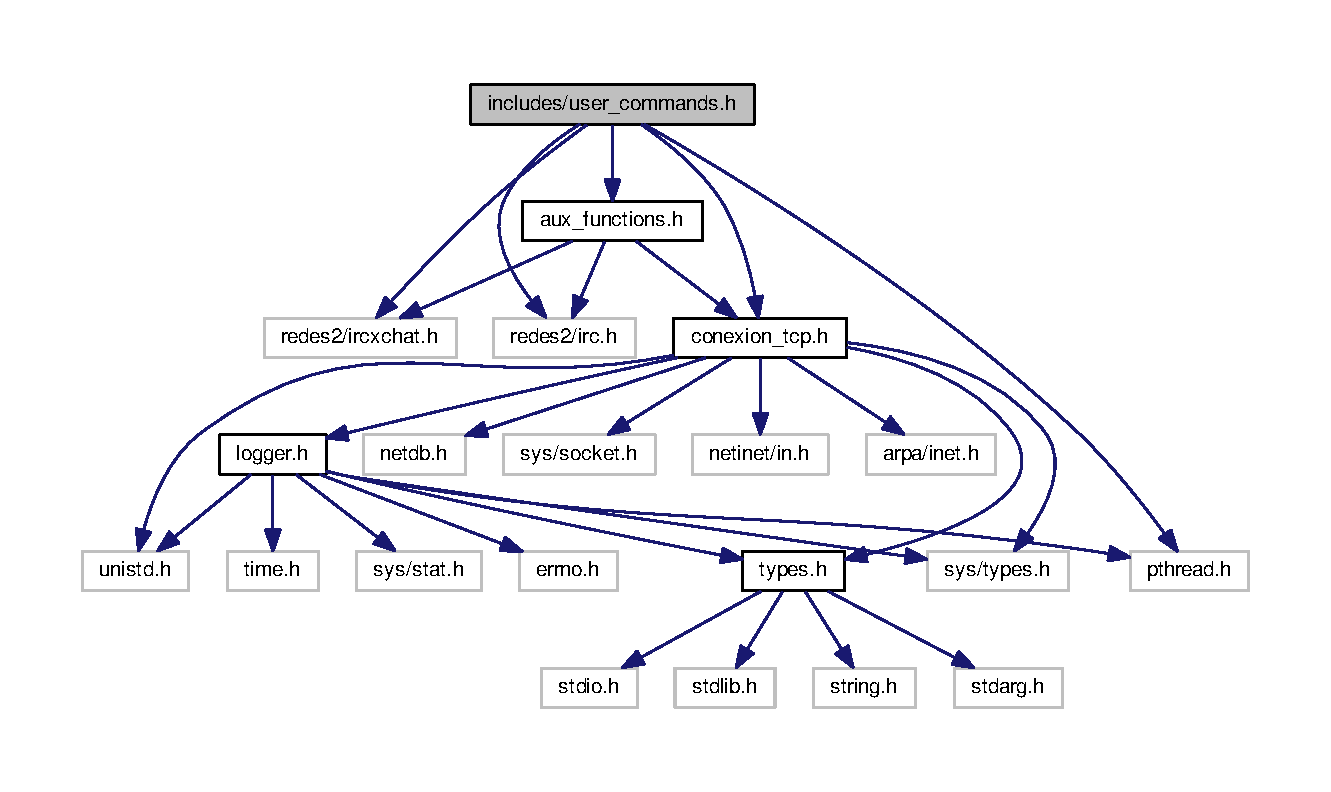
\includegraphics[width=350pt]{user__commands_8h__incl}
\end{center}
\end{figure}
This graph shows which files directly or indirectly include this file\-:
\nopagebreak
\begin{figure}[H]
\begin{center}
\leavevmode
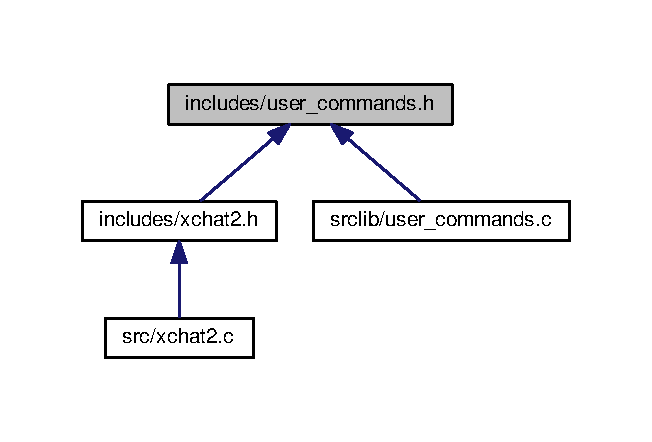
\includegraphics[width=313pt]{user__commands_8h__dep__incl}
\end{center}
\end{figure}
\subsection*{Typedefs}
\begin{DoxyCompactItemize}
\item 
typedef int($\ast$ \hyperlink{user__commands_8h_aa28997a055736f12ce4f2db646ef7749}{p\-\_\-funcion} )(char $\ast$)
\end{DoxyCompactItemize}
\subsection*{Functions}
\begin{DoxyCompactItemize}
\item 
int \hyperlink{user__commands_8h_a4dd6e13bec86782e1c29bc67c6040b95}{punotice} (char $\ast$command)
\begin{DoxyCompactList}\small\item\em Comando de usuario N\-O\-T\-I\-C\-E Send a notice to a user, channel or server.
\begin{DoxyItemize}
\item N\-O\-T\-I\-C\-E $<$nick$>$ $<$text$>$ Send a notice to a user. Ex\-: /\-N\-O\-T\-I\-C\-E Blah hi, how are you?
\item N\-O\-T\-I\-C\-E $<$\#channel$>$ $<$text$>$ Send a notice to a channel. Ex\-: /\-N\-O\-T\-I\-C\-E \#room Hi all, this is annoying. 
\end{DoxyItemize}\end{DoxyCompactList}\item 
int \hyperlink{user__commands_8h_a365e633f087eadb08ef23ec8d20abaf6}{pucycle} (char $\ast$command)
\begin{DoxyCompactList}\small\item\em Comando de usuario C\-Y\-C\-L\-E Cycles the given channel(s). This command is equivilent to sending a P\-A\-R\-T then a J\-O\-I\-N command.
\begin{DoxyItemize}
\item Syntax\-: C\-Y\-C\-L\-E $<$chan1$>$,$<$chan2$>$,$<$chan3$>$ ... 
\end{DoxyItemize}\end{DoxyCompactList}\item 
int \hyperlink{user__commands_8h_a4d9661d482929bb458b85e70c6170d74}{pumotd} (char $\ast$command)
\begin{DoxyCompactList}\small\item\em Comando de usuario M\-O\-T\-D Displays the Message Of The Day of the I\-R\-C Server you are logged onto.
\begin{DoxyItemize}
\item Syntax\-: M\-O\-T\-D M\-O\-T\-D $<$server$>$ 
\end{DoxyItemize}\end{DoxyCompactList}\item 
int \hyperlink{user__commands_8h_a8e0f94275dfaa1e7bc564d3555b9402e}{pulusers} (char $\ast$command)
\begin{DoxyCompactList}\small\item\em Comando de usuario L\-U\-S\-E\-R\-S Provides Local and Global user information (Such as Current and Maximum user count).
\begin{DoxyItemize}
\item Syntax\-: L\-U\-S\-E\-R\-S \mbox{[}server\mbox{]}. 
\end{DoxyItemize}\end{DoxyCompactList}\item 
int \hyperlink{user__commands_8h_a448b3ec98632740523ee7a20c5bc81dd}{pumode} (char $\ast$command)
\item 
int \hyperlink{user__commands_8h_a1af5de7d9cb449f78a7f511d28c64ba9}{pupartall} (char $\ast$command)
\item 
int \hyperlink{user__commands_8h_ae822b5550f387a177b98ec2c98e26b2d}{puback} (char $\ast$command)
\item 
int \hyperlink{user__commands_8h_a8a3e6d36d02bc24a451f806de272c691}{puunaway} (char $\ast$command)
\item 
int \hyperlink{user__commands_8h_ab51cd004b9746694fb19829952779c6b}{puoper} (char $\ast$command)
\item 
int \hyperlink{user__commands_8h_a8b10f809b49ed8686a693efc87f144e5}{puban} (char $\ast$command)
\item 
int \hyperlink{user__commands_8h_a546e9e7086ec6347e0d3dffef5f11694}{pufsend} (char $\ast$command)
\item 
int \hyperlink{user__commands_8h_aea754f971df97746d113aaedc41c8cbf}{pufaccept} (char $\ast$command)
\item 
int \hyperlink{user__commands_8h_a79c4db4db149aa147f4b508b999febe2}{pufclose} (char $\ast$command)
\item 
int \hyperlink{user__commands_8h_a0a15138d8927dd543805edcc035b8132}{putopic} (char $\ast$command)
\item 
int \hyperlink{user__commands_8h_ac7817f0890faebb4fb8f13cc6ee5c838}{pukick} (char $\ast$command)
\item 
int \hyperlink{user__commands_8h_a856ef0800c85e0f20fad89ff8070b3f9}{puinvite} (char $\ast$command)
\begin{DoxyCompactList}\small\item\em Comando de usuario I\-N\-V\-I\-T\-E Sends a user an Invitation to join a particular channel. If the channel is +i, you must be an Operator to use this command, otherwise any user may use the command. Invite without parameters lists the channels you have been invited to.
\begin{DoxyItemize}
\item Syntax\-: I\-N\-V\-I\-T\-E $<$user$>$ $<$channel$>$ 
\end{DoxyItemize}\end{DoxyCompactList}\item 
int \hyperlink{user__commands_8h_a08bd5900f288bfb5712d3f5ca6e624b6}{puwhois} (char $\ast$command)
\begin{DoxyCompactList}\small\item\em Comando de usuario W\-H\-O\-I\-S Shows information about the user in question, such as their \char`\"{}\-Name\char`\"{}, channels they are currently in, their hostmask, etc.
\begin{DoxyItemize}
\item Syntax\-: W\-H\-O\-I\-S $<$user$>$ 
\end{DoxyItemize}\end{DoxyCompactList}\item 
int \hyperlink{user__commands_8h_a84e1c4ef3c7307f98a3d2267ae0ce121}{puaway} (char $\ast$command)
\begin{DoxyCompactList}\small\item\em Comando de usuario A\-W\-A\-Y. \end{DoxyCompactList}\item 
int \hyperlink{user__commands_8h_a93cab9103f7f4815ff20b47dcf0c117c}{punick} (char $\ast$command)
\begin{DoxyCompactList}\small\item\em Comando de usuario N\-I\-C\-K Changes your \char`\"{}\-Online Identity\char`\"{} on a server. All those in the channel you are in will be alerted of your nickname change.
\begin{DoxyItemize}
\item Syntax\-: N\-I\-C\-K $<$new nickname$>$=\char`\"{}\char`\"{}$>$ 
\end{DoxyItemize}\end{DoxyCompactList}\item 
int \hyperlink{user__commands_8h_ad738a7d361fe18d7774bab370a4454a8}{puquit} (char $\ast$command)
\begin{DoxyCompactList}\small\item\em Comando de usuario Q\-U\-I\-T En principio solo se llama con\-: \end{DoxyCompactList}\item 
int \hyperlink{user__commands_8h_a2d0a8c0565fc24fdd54dc68de05e6474}{puleave} (char $\ast$command)
\item 
int \hyperlink{user__commands_8h_adc5c5d5b72106761066833022c9bc83d}{pupart} (char $\ast$command)
\begin{DoxyCompactList}\small\item\em Comando de usuario P\-A\-R\-T Used to part (or leave) a channel you currently occupy. All those in the channel will be notified of your departure. If you specify a reason it will be displayed to the users on the channel
\begin{DoxyItemize}
\item Syntax\-: P\-A\-R\-T $<$chan$>$,$<$chan2$>$,$<$chan3$>$,$<$chan4$>$ $<$reason$>$ 
\end{DoxyItemize}\end{DoxyCompactList}\item 
int \hyperlink{user__commands_8h_add059d444d6e29f6e18f67bda6c21878}{pujoin} (char $\ast$command)
\begin{DoxyCompactList}\small\item\em Comando de usuario J\-O\-I\-N. \end{DoxyCompactList}\item 
int \hyperlink{user__commands_8h_aef4e57bf112f9c4a2d51b1a314df0b63}{puwho} (char $\ast$command)
\begin{DoxyCompactList}\small\item\em Comando de usuario W\-H\-O. \end{DoxyCompactList}\item 
int \hyperlink{user__commands_8h_abaae116595df34db33e65e3d9d225103}{punames} (char $\ast$command)
\begin{DoxyCompactList}\small\item\em Comando de usuario N\-A\-M\-E\-S. \end{DoxyCompactList}\item 
int \hyperlink{user__commands_8h_a322cdf0baafadcd1784ab6c8f6d48f04}{pumsg} (char $\ast$command)
\begin{DoxyCompactList}\small\item\em Comando de usuario M\-S\-G y P\-R\-I\-V\-M\-S\-G. \end{DoxyCompactList}\item 
int \hyperlink{user__commands_8h_a2da90a4a7474a7a220ab1588dedd7ef4}{pulist} (char $\ast$command)
\begin{DoxyCompactList}\small\item\em Comando de usuario L\-I\-S\-T. \end{DoxyCompactList}\item 
int \hyperlink{user__commands_8h_a9b25b9a254568a07285fc068e01d9919}{puhelp} (char $\ast$command)
\begin{DoxyCompactList}\small\item\em Comando de usuario H\-E\-L\-P. \end{DoxyCompactList}\item 
int \hyperlink{user__commands_8h_a05216fb56a43c8fa44b5bc726692b064}{pdefault} (char $\ast$command)
\begin{DoxyCompactList}\small\item\em Comando desconocido para el cliente. \end{DoxyCompactList}\item 
int \hyperlink{user__commands_8h_a8149f7beb37fd789f142acb2113efd1c}{puquery} (char $\ast$command)
\begin{DoxyCompactList}\small\item\em Comando de usuario Q\-U\-E\-R\-Y Use the \char`\"{}/query $<$user$>$\char`\"{} command to specify that every message you type should be directed to a single user. \end{DoxyCompactList}\end{DoxyCompactItemize}
\subsection*{Variables}
\begin{DoxyCompactItemize}
\item 
int \hyperlink{user__commands_8h_acd63fb8dbd9439219e2db08dfc173aa0}{sockfd\-\_\-user}
\item 
char \hyperlink{user__commands_8h_a7e2f32e47f3780a66e19651d8e79bced}{nick\-\_\-user} \mbox{[}\hyperlink{types_8h_ae7e715c270481406658bbd2bafa2897f}{M\-A\-X\-D\-A\-T\-A}\mbox{]}
\item 
pthread\-\_\-t \hyperlink{user__commands_8h_ab5efd1efa144e252f4c5312ae57bea2e}{recv\-\_\-tid}
\end{DoxyCompactItemize}


\subsection{Detailed Description}
Declaraciones de funciones, definición de tipos\-: implementación de funciones I\-R\-C de usuario. \begin{DoxyAuthor}{Author}
Alfonso Sebares 

Beatriz de Pablo 

Celia Mateos 
\end{DoxyAuthor}
\begin{DoxyDate}{Date}
20/03/17 
\end{DoxyDate}


\subsection{Typedef Documentation}
\hypertarget{user__commands_8h_aa28997a055736f12ce4f2db646ef7749}{\index{user\-\_\-commands.\-h@{user\-\_\-commands.\-h}!p\-\_\-funcion@{p\-\_\-funcion}}
\index{p\-\_\-funcion@{p\-\_\-funcion}!user_commands.h@{user\-\_\-commands.\-h}}
\subsubsection[{p\-\_\-funcion}]{\setlength{\rightskip}{0pt plus 5cm}typedef int($\ast$ p\-\_\-funcion)(char $\ast$)}}\label{user__commands_8h_aa28997a055736f12ce4f2db646ef7749}
definicion del tipo de puntero a array de funciones 

\subsection{Function Documentation}
\hypertarget{user__commands_8h_a05216fb56a43c8fa44b5bc726692b064}{\index{user\-\_\-commands.\-h@{user\-\_\-commands.\-h}!pdefault@{pdefault}}
\index{pdefault@{pdefault}!user_commands.h@{user\-\_\-commands.\-h}}
\subsubsection[{pdefault}]{\setlength{\rightskip}{0pt plus 5cm}int pdefault (
\begin{DoxyParamCaption}
\item[{char $\ast$}]{command}
\end{DoxyParamCaption}
)}}\label{user__commands_8h_a05216fb56a43c8fa44b5bc726692b064}


Comando desconocido para el cliente. 


\begin{DoxyParams}{Parameters}
{\em command} & cadena introducida por el usuario en el campo de texto \\
\hline
\end{DoxyParams}
\begin{DoxyReturn}{Returns}
O\-K si todo es correcto, E\-R\-R si se produce un error 
\end{DoxyReturn}

\begin{DoxyCode}
369                            \{ 
370         IRCInterface\_WriteSystem(\hyperlink{user__commands_8h_a7e2f32e47f3780a66e19651d8e79bced}{nick\_user}, \textcolor{stringliteral}{"No se ha podido ejecutar el comando: "});
371         IRCInterface\_WriteSystem(\hyperlink{user__commands_8h_a7e2f32e47f3780a66e19651d8e79bced}{nick\_user}, command);
372         \textcolor{keywordflow}{return} 0;
373 \}
\end{DoxyCode}
\hypertarget{user__commands_8h_a84e1c4ef3c7307f98a3d2267ae0ce121}{\index{user\-\_\-commands.\-h@{user\-\_\-commands.\-h}!puaway@{puaway}}
\index{puaway@{puaway}!user_commands.h@{user\-\_\-commands.\-h}}
\subsubsection[{puaway}]{\setlength{\rightskip}{0pt plus 5cm}int puaway (
\begin{DoxyParamCaption}
\item[{char $\ast$}]{command}
\end{DoxyParamCaption}
)}}\label{user__commands_8h_a84e1c4ef3c7307f98a3d2267ae0ce121}


Comando de usuario A\-W\-A\-Y. 

Sets your online status to \char`\"{}\-Away\char`\"{}.
\begin{DoxyItemize}
\item Syntax\-: A\-W\-A\-Y $<$reason$>$ (Sets you Away with the reason given) A\-W\-A\-Y (Un-\/\-Sets you as Away) Example\-: A\-W\-A\-Y Lunch time! 
\begin{DoxyParams}{Parameters}
{\em command} & cadena introducida por el usuario en el campo de texto \\
\hline
\end{DoxyParams}
\begin{DoxyReturn}{Returns}
O\-K si todo es correcto, E\-R\-R si se produce un error 
\end{DoxyReturn}

\end{DoxyItemize}
\begin{DoxyCode}
410                          \{
411         \textcolor{keywordtype}{char}* command\_enviar;
412         \textcolor{keywordtype}{char} *reason;
413         \textcolor{keywordtype}{int} free\_f = 0;
414 
415         IRCUserParse\_Away (command, &reason);
416         \textcolor{comment}{/*}
417 \textcolor{comment}{        if(reason == NULL || strlen(reason) == 0)\{}
418 \textcolor{comment}{                reason = "afk";}
419 \textcolor{comment}{                free\_f = 1;}
420 \textcolor{comment}{        \}*/}
421 
422         IRCMsg\_Away (&command\_enviar, NULL, reason);
423         g\_print(\textcolor{stringliteral}{"\(\backslash\)t Mensaje a enviar command\_enviar en AWAY: %s \(\backslash\)n"},command\_enviar);
424 
425         \hyperlink{conexion__tcp_8h_ab9468ce1338cfca5736ab407ba155f55}{enviarDatos}(\hyperlink{aux__functions_8h_acd63fb8dbd9439219e2db08dfc173aa0}{sockfd\_user}, command\_enviar, strlen(command\_enviar));
426         IRCInterface\_PlaneRegisterOutMessage(command\_enviar);
427         
428         \textcolor{keywordflow}{if}(free\_f)
429                 \hyperlink{aux__functions_8h_a2480cc4793bf25a16cc731dc9d033582}{mfree}(1, command\_enviar);
430         \textcolor{keywordflow}{else}
431                 \hyperlink{aux__functions_8h_a2480cc4793bf25a16cc731dc9d033582}{mfree}(2, command\_enviar, reason);
432         \textcolor{keywordflow}{return} \hyperlink{daemon_8h_aba51915c87d64af47fb1cc59348961c9}{OK};
433 \}
\end{DoxyCode}


Here is the call graph for this function\-:
\nopagebreak
\begin{figure}[H]
\begin{center}
\leavevmode
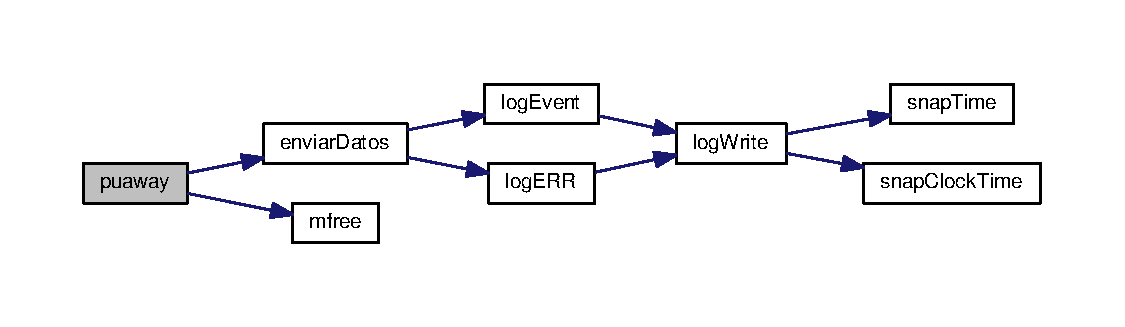
\includegraphics[width=350pt]{user__commands_8h_a84e1c4ef3c7307f98a3d2267ae0ce121_cgraph}
\end{center}
\end{figure}


\hypertarget{user__commands_8h_ae822b5550f387a177b98ec2c98e26b2d}{\index{user\-\_\-commands.\-h@{user\-\_\-commands.\-h}!puback@{puback}}
\index{puback@{puback}!user_commands.h@{user\-\_\-commands.\-h}}
\subsubsection[{puback}]{\setlength{\rightskip}{0pt plus 5cm}int puback (
\begin{DoxyParamCaption}
\item[{char $\ast$}]{command}
\end{DoxyParamCaption}
)}}\label{user__commands_8h_ae822b5550f387a177b98ec2c98e26b2d}

\begin{DoxyCode}
29 \{ \textcolor{keywordflow}{return} -1; \}
\end{DoxyCode}
\hypertarget{user__commands_8h_a8b10f809b49ed8686a693efc87f144e5}{\index{user\-\_\-commands.\-h@{user\-\_\-commands.\-h}!puban@{puban}}
\index{puban@{puban}!user_commands.h@{user\-\_\-commands.\-h}}
\subsubsection[{puban}]{\setlength{\rightskip}{0pt plus 5cm}int puban (
\begin{DoxyParamCaption}
\item[{char $\ast$}]{command}
\end{DoxyParamCaption}
)}}\label{user__commands_8h_a8b10f809b49ed8686a693efc87f144e5}

\begin{DoxyCode}
32 \{ \textcolor{keywordflow}{return} -1; \} \textcolor{comment}{// ya se envia con los botones}
\end{DoxyCode}
\hypertarget{user__commands_8h_a365e633f087eadb08ef23ec8d20abaf6}{\index{user\-\_\-commands.\-h@{user\-\_\-commands.\-h}!pucycle@{pucycle}}
\index{pucycle@{pucycle}!user_commands.h@{user\-\_\-commands.\-h}}
\subsubsection[{pucycle}]{\setlength{\rightskip}{0pt plus 5cm}int pucycle (
\begin{DoxyParamCaption}
\item[{char $\ast$}]{command}
\end{DoxyParamCaption}
)}}\label{user__commands_8h_a365e633f087eadb08ef23ec8d20abaf6}


Comando de usuario C\-Y\-C\-L\-E Cycles the given channel(s). This command is equivilent to sending a P\-A\-R\-T then a J\-O\-I\-N command.
\begin{DoxyItemize}
\item Syntax\-: C\-Y\-C\-L\-E $<$chan1$>$,$<$chan2$>$,$<$chan3$>$ ... 
\end{DoxyItemize}


\begin{DoxyParams}{Parameters}
{\em command} & cadena introducida por el usuario en el campo de texto \\
\hline
\end{DoxyParams}
\begin{DoxyReturn}{Returns}
O\-K si todo es correcto, E\-R\-R si se produce un error 
\end{DoxyReturn}

\begin{DoxyCode}
632                           \{
633 
634         \textcolor{keywordtype}{char}* respuesta = NULL;
635     \textcolor{keywordtype}{char}** target;
636     \textcolor{keywordtype}{int} numchannels=0;
637     \textcolor{keywordtype}{int} i ;
638 
639     IRCUserParse\_Cycle (command, &target, &numchannels);
640     \textcolor{keywordflow}{for} (i = 0; i< numchannels; i++)\{
641         IRCMsg\_Part (&respuesta, NULL, target[i], \textcolor{stringliteral}{"Saliendo"});
642                 \hyperlink{conexion__tcp_8h_ab9468ce1338cfca5736ab407ba155f55}{enviarDatos}(\hyperlink{aux__functions_8h_acd63fb8dbd9439219e2db08dfc173aa0}{sockfd\_user}, respuesta, strlen(respuesta));
643         IRCInterface\_PlaneRegisterOutMessage (respuesta);
644         free(respuesta);
645         IRCMsg\_Join(&respuesta, NULL, target[i], NULL, NULL);
646                 \hyperlink{conexion__tcp_8h_ab9468ce1338cfca5736ab407ba155f55}{enviarDatos}(\hyperlink{aux__functions_8h_acd63fb8dbd9439219e2db08dfc173aa0}{sockfd\_user}, respuesta, strlen(respuesta));
647         IRCInterface\_PlaneRegisterOutMessage (respuesta);
648         free(respuesta);
649     \}
650 
651     \textcolor{keywordflow}{return} \hyperlink{daemon_8h_aba51915c87d64af47fb1cc59348961c9}{OK};   
652 \}
\end{DoxyCode}


Here is the call graph for this function\-:
\nopagebreak
\begin{figure}[H]
\begin{center}
\leavevmode
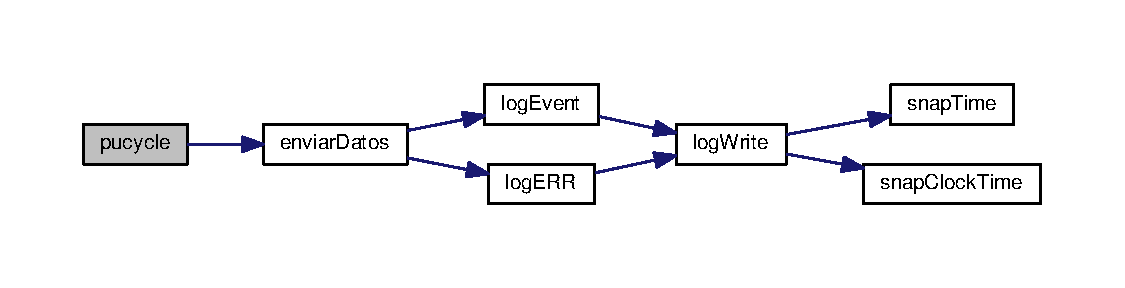
\includegraphics[width=350pt]{user__commands_8h_a365e633f087eadb08ef23ec8d20abaf6_cgraph}
\end{center}
\end{figure}


\hypertarget{user__commands_8h_aea754f971df97746d113aaedc41c8cbf}{\index{user\-\_\-commands.\-h@{user\-\_\-commands.\-h}!pufaccept@{pufaccept}}
\index{pufaccept@{pufaccept}!user_commands.h@{user\-\_\-commands.\-h}}
\subsubsection[{pufaccept}]{\setlength{\rightskip}{0pt plus 5cm}int pufaccept (
\begin{DoxyParamCaption}
\item[{char $\ast$}]{command}
\end{DoxyParamCaption}
)}}\label{user__commands_8h_aea754f971df97746d113aaedc41c8cbf}

\begin{DoxyCode}
34 \{ \textcolor{keywordflow}{return} -1; \} \textcolor{comment}{//se envia con los ficheros}
\end{DoxyCode}
\hypertarget{user__commands_8h_a79c4db4db149aa147f4b508b999febe2}{\index{user\-\_\-commands.\-h@{user\-\_\-commands.\-h}!pufclose@{pufclose}}
\index{pufclose@{pufclose}!user_commands.h@{user\-\_\-commands.\-h}}
\subsubsection[{pufclose}]{\setlength{\rightskip}{0pt plus 5cm}int pufclose (
\begin{DoxyParamCaption}
\item[{char $\ast$}]{command}
\end{DoxyParamCaption}
)}}\label{user__commands_8h_a79c4db4db149aa147f4b508b999febe2}

\begin{DoxyCode}
35 \{ \textcolor{keywordflow}{return} -1; \} \textcolor{comment}{//se envia con los ficheros}
\end{DoxyCode}
\hypertarget{user__commands_8h_a546e9e7086ec6347e0d3dffef5f11694}{\index{user\-\_\-commands.\-h@{user\-\_\-commands.\-h}!pufsend@{pufsend}}
\index{pufsend@{pufsend}!user_commands.h@{user\-\_\-commands.\-h}}
\subsubsection[{pufsend}]{\setlength{\rightskip}{0pt plus 5cm}int pufsend (
\begin{DoxyParamCaption}
\item[{char $\ast$}]{command}
\end{DoxyParamCaption}
)}}\label{user__commands_8h_a546e9e7086ec6347e0d3dffef5f11694}

\begin{DoxyCode}
33 \{ \textcolor{keywordflow}{return} -1; \} \textcolor{comment}{//se envia con los ficheros}
\end{DoxyCode}
\hypertarget{user__commands_8h_a9b25b9a254568a07285fc068e01d9919}{\index{user\-\_\-commands.\-h@{user\-\_\-commands.\-h}!puhelp@{puhelp}}
\index{puhelp@{puhelp}!user_commands.h@{user\-\_\-commands.\-h}}
\subsubsection[{puhelp}]{\setlength{\rightskip}{0pt plus 5cm}int puhelp (
\begin{DoxyParamCaption}
\item[{char $\ast$}]{command}
\end{DoxyParamCaption}
)}}\label{user__commands_8h_a9b25b9a254568a07285fc068e01d9919}


Comando de usuario H\-E\-L\-P. 


\begin{DoxyParams}{Parameters}
{\em command} & cadena introducida por el usuario en el campo de texto \\
\hline
\end{DoxyParams}
\begin{DoxyReturn}{Returns}
O\-K si todo es correcto, E\-R\-R si se produce un error 
\end{DoxyReturn}

\begin{DoxyCode}
351                          \{
352         \textcolor{keywordtype}{char}* comando;
353         \textcolor{keywordtype}{char} command\_enviar[\hyperlink{types_8h_ae7e715c270481406658bbd2bafa2897f}{MAXDATA}];
354 
355         IRCUserParse\_Help (command, &comando);
356         sprintf(command\_enviar, \textcolor{stringliteral}{"HELP %s\(\backslash\)r\(\backslash\)n"}, comando?comando:\textcolor{stringliteral}{""});
357         \hyperlink{conexion__tcp_8h_ab9468ce1338cfca5736ab407ba155f55}{enviarDatos}(\hyperlink{aux__functions_8h_acd63fb8dbd9439219e2db08dfc173aa0}{sockfd\_user}, command\_enviar, strlen(command\_enviar)); 
358         IRCInterface\_PlaneRegisterOutMessage(command\_enviar);
359         \hyperlink{aux__functions_8h_a2480cc4793bf25a16cc731dc9d033582}{mfree}(1, comando);
360         \textcolor{keywordflow}{return} \hyperlink{daemon_8h_aba51915c87d64af47fb1cc59348961c9}{OK};
361 \}
\end{DoxyCode}


Here is the call graph for this function\-:
\nopagebreak
\begin{figure}[H]
\begin{center}
\leavevmode
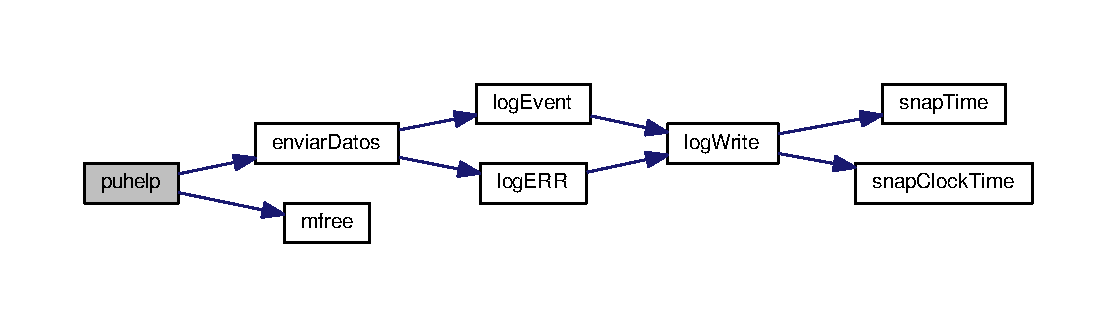
\includegraphics[width=350pt]{user__commands_8h_a9b25b9a254568a07285fc068e01d9919_cgraph}
\end{center}
\end{figure}


\hypertarget{user__commands_8h_a856ef0800c85e0f20fad89ff8070b3f9}{\index{user\-\_\-commands.\-h@{user\-\_\-commands.\-h}!puinvite@{puinvite}}
\index{puinvite@{puinvite}!user_commands.h@{user\-\_\-commands.\-h}}
\subsubsection[{puinvite}]{\setlength{\rightskip}{0pt plus 5cm}int puinvite (
\begin{DoxyParamCaption}
\item[{char $\ast$}]{command}
\end{DoxyParamCaption}
)}}\label{user__commands_8h_a856ef0800c85e0f20fad89ff8070b3f9}


Comando de usuario I\-N\-V\-I\-T\-E Sends a user an Invitation to join a particular channel. If the channel is +i, you must be an Operator to use this command, otherwise any user may use the command. Invite without parameters lists the channels you have been invited to.
\begin{DoxyItemize}
\item Syntax\-: I\-N\-V\-I\-T\-E $<$user$>$ $<$channel$>$ 
\end{DoxyItemize}


\begin{DoxyParams}{Parameters}
{\em command} & cadena introducida por el usuario en el campo de texto \\
\hline
\end{DoxyParams}
\begin{DoxyReturn}{Returns}
O\-K si todo es correcto, E\-R\-R si se produce un error 
\end{DoxyReturn}

\begin{DoxyCode}
470                            \{
471 
472         \textcolor{keywordtype}{char}* command\_enviar = NULL, *prefix = NULL, *nick = NULL, *channel = NULL;
473 
474         g\_print(\textcolor{stringliteral}{"\(\backslash\)t Mensaje reciido en UINVITE: %s \(\backslash\)n"},command);
475 
476         IRCParse\_Invite (command, &prefix, &nick, &channel); \textcolor{comment}{//la parseo con esta funcion del server porque
       no hay del user}
477         g\_print(\textcolor{stringliteral}{"\(\backslash\)t prefix: %s \(\backslash\)n"},prefix);
478         g\_print(\textcolor{stringliteral}{"\(\backslash\)t nick: %s \(\backslash\)n"},nick);
479         g\_print(\textcolor{stringliteral}{"\(\backslash\)t channel: %s \(\backslash\)n"},channel);
480 
481         IRCMsg\_Invite (&command\_enviar, prefix, nick, channel);
482         g\_print(\textcolor{stringliteral}{"\(\backslash\)t Mensaje a enviar en UINVITE: %s \(\backslash\)n"}, command\_enviar);
483 
484         \hyperlink{conexion__tcp_8h_ab9468ce1338cfca5736ab407ba155f55}{enviarDatos}(\hyperlink{aux__functions_8h_acd63fb8dbd9439219e2db08dfc173aa0}{sockfd\_user}, command\_enviar, strlen(command\_enviar));
485         IRCInterface\_PlaneRegisterOutMessage(command\_enviar);
486         \hyperlink{aux__functions_8h_a2480cc4793bf25a16cc731dc9d033582}{mfree}(4, command\_enviar, channel, nick, prefix);
487         \textcolor{keywordflow}{return} \hyperlink{daemon_8h_aba51915c87d64af47fb1cc59348961c9}{OK};
488 \}
\end{DoxyCode}


Here is the call graph for this function\-:
\nopagebreak
\begin{figure}[H]
\begin{center}
\leavevmode
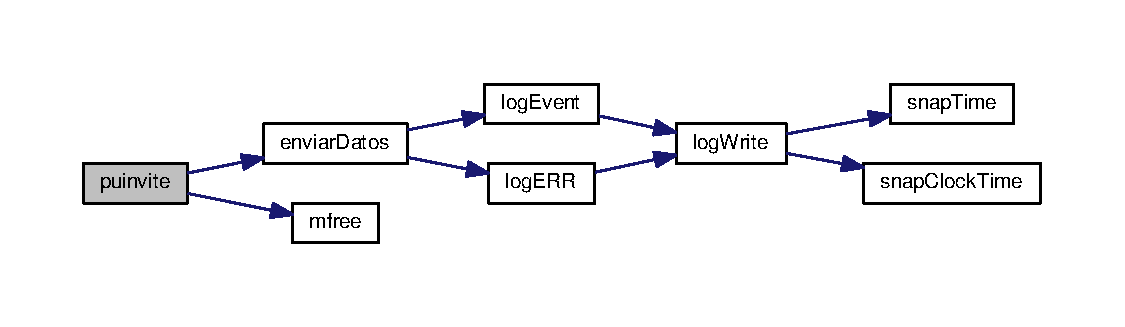
\includegraphics[width=350pt]{user__commands_8h_a856ef0800c85e0f20fad89ff8070b3f9_cgraph}
\end{center}
\end{figure}


\hypertarget{user__commands_8h_add059d444d6e29f6e18f67bda6c21878}{\index{user\-\_\-commands.\-h@{user\-\_\-commands.\-h}!pujoin@{pujoin}}
\index{pujoin@{pujoin}!user_commands.h@{user\-\_\-commands.\-h}}
\subsubsection[{pujoin}]{\setlength{\rightskip}{0pt plus 5cm}int pujoin (
\begin{DoxyParamCaption}
\item[{char $\ast$}]{command}
\end{DoxyParamCaption}
)}}\label{user__commands_8h_add059d444d6e29f6e18f67bda6c21878}


Comando de usuario J\-O\-I\-N. 


\begin{DoxyParams}{Parameters}
{\em command} & cadena introducida por el usuario en el campo de texto \\
\hline
\end{DoxyParams}
\begin{DoxyReturn}{Returns}
O\-K si todo es correcto, E\-R\-R si se produce un error 
\end{DoxyReturn}

\begin{DoxyCode}
131                          \{ 
132 
133         \textcolor{keywordtype}{long} ret = -1;
134         \textcolor{keywordtype}{int} retorno = -1;
135 
136         \textcolor{keywordtype}{char}* key = NULL;
137         \textcolor{keywordtype}{char}* msg = NULL;
138         \textcolor{keywordtype}{char}* channels = NULL;
139         \textcolor{keywordtype}{char}* passwords = NULL;
140         \textcolor{keywordtype}{char}* command\_enviar = NULL;
141         \textcolor{keywordtype}{char}* prefix = NULL;
142         \textcolor{keywordtype}{char} canales\_y\_passwords [\hyperlink{types_8h_ae7e715c270481406658bbd2bafa2897f}{MAXDATA}] = \{0\};
143 
144         g\_print(\hyperlink{types_8h_af54a5a977c0c499323d656315f008ee0}{MAG} \textcolor{stringliteral}{"\(\backslash\)n<< [user command] UJOIN - command = %s\(\backslash\)n"} \hyperlink{types_8h_ab702106cf3b3e96750b6845ded4e0299}{RESET}, command);
145 
146         ret = IRCUserParse\_Join(command, &channels, &passwords);
147         \textcolor{keywordflow}{if}(ret != IRC\_OK)\{
148                 g\_print(\hyperlink{types_8h_a8d23feea868a983c8c2b661e1e16972f}{RED} \textcolor{stringliteral}{"ERROR - In pujoin: IRCUserParse\_Join no devolvio IRC\_OK\(\backslash\)n"} 
      \hyperlink{types_8h_ab702106cf3b3e96750b6845ded4e0299}{RESET});
149                 \textcolor{keywordflow}{return} -1;
150         \}
151         g\_print(\textcolor{stringliteral}{"\(\backslash\)t command: %s \(\backslash\)n"},command);
152         g\_print(\textcolor{stringliteral}{"\(\backslash\)t channels : %s \(\backslash\)n"},channels);
153         g\_print(\textcolor{stringliteral}{"\(\backslash\)t passwords : %s \(\backslash\)n"},passwords);
154 
155         sprintf(canales\_y\_passwords,\textcolor{stringliteral}{"%s %s"},channels,passwords?passwords:\textcolor{stringliteral}{""});
156 
157         \textcolor{comment}{//enviar varios canales}
158         ret = IRCMsg\_Join (&command\_enviar, prefix, canales\_y\_passwords, key, msg);
159         \textcolor{keywordflow}{if}(ret != IRC\_OK)\{
160                 g\_print(\hyperlink{types_8h_a8d23feea868a983c8c2b661e1e16972f}{RED} \textcolor{stringliteral}{"ERROR - In pujoin: IRCMsg\_Join no devolvio IRC\_OK\(\backslash\)n"} 
      \hyperlink{types_8h_ab702106cf3b3e96750b6845ded4e0299}{RESET});
161                 \textcolor{keywordflow}{return} -1;
162         \}
163         g\_print(\textcolor{stringliteral}{"\(\backslash\)t Mensaje a enviar command\_enviar: %s \(\backslash\)n"},command\_enviar);
164         
165         retorno = \hyperlink{conexion__tcp_8h_ab9468ce1338cfca5736ab407ba155f55}{enviarDatos}(\hyperlink{aux__functions_8h_acd63fb8dbd9439219e2db08dfc173aa0}{sockfd\_user},command\_enviar, strlen(command\_enviar));
166         \textcolor{keywordflow}{if}(retorno < 0)\{
167                 g\_print(\hyperlink{types_8h_a8d23feea868a983c8c2b661e1e16972f}{RED} \textcolor{stringliteral}{"ERROR - In pujoin: enviarDatos() devolvio error (ver secuencia en .log)\(\backslash\)n\(\backslash\)t
      \(\backslash\)tEl cliente se cerrará.\(\backslash\)n"} \hyperlink{types_8h_ab702106cf3b3e96750b6845ded4e0299}{RESET});
168                 exit(1);
169         \}
170         \textcolor{keywordflow}{if}(retorno == 0)\{ \textcolor{comment}{//timeout }
171                 g\_print(\hyperlink{types_8h_a8d23feea868a983c8c2b661e1e16972f}{RED} \textcolor{stringliteral}{"ERROR - In pujoin: enviarDatos() envió 0 Bytes(ver secuencia en .log)\(\backslash\)n\(\backslash\)t\(\backslash\)t
      (Timeout de conexión probablemente)\(\backslash\)n"} \hyperlink{types_8h_ab702106cf3b3e96750b6845ded4e0299}{RESET});
172                 exit(1);
173         \}
174 
175         IRCInterface\_PlaneRegisterOutMessage(command\_enviar);   
176         \hyperlink{aux__functions_8h_a2480cc4793bf25a16cc731dc9d033582}{mfree}(6, command\_enviar, channels, passwords, prefix, key, msg);
177         \textcolor{keywordflow}{return} \hyperlink{daemon_8h_aba51915c87d64af47fb1cc59348961c9}{OK}; 
178 \}
\end{DoxyCode}


Here is the call graph for this function\-:
\nopagebreak
\begin{figure}[H]
\begin{center}
\leavevmode
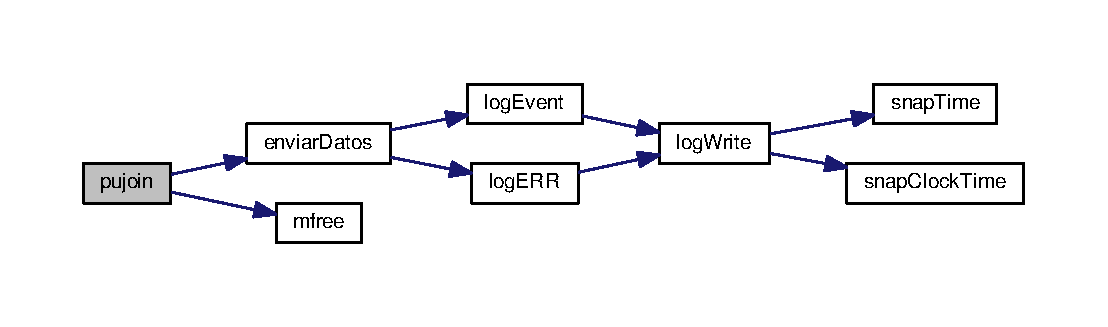
\includegraphics[width=350pt]{user__commands_8h_add059d444d6e29f6e18f67bda6c21878_cgraph}
\end{center}
\end{figure}


\hypertarget{user__commands_8h_ac7817f0890faebb4fb8f13cc6ee5c838}{\index{user\-\_\-commands.\-h@{user\-\_\-commands.\-h}!pukick@{pukick}}
\index{pukick@{pukick}!user_commands.h@{user\-\_\-commands.\-h}}
\subsubsection[{pukick}]{\setlength{\rightskip}{0pt plus 5cm}int pukick (
\begin{DoxyParamCaption}
\item[{char $\ast$}]{command}
\end{DoxyParamCaption}
)}}\label{user__commands_8h_ac7817f0890faebb4fb8f13cc6ee5c838}

\begin{DoxyCode}
37 \{ \textcolor{keywordflow}{return} -1; \} \textcolor{comment}{//se envia con los botones}
\end{DoxyCode}
\hypertarget{user__commands_8h_a2d0a8c0565fc24fdd54dc68de05e6474}{\index{user\-\_\-commands.\-h@{user\-\_\-commands.\-h}!puleave@{puleave}}
\index{puleave@{puleave}!user_commands.h@{user\-\_\-commands.\-h}}
\subsubsection[{puleave}]{\setlength{\rightskip}{0pt plus 5cm}int puleave (
\begin{DoxyParamCaption}
\item[{char $\ast$}]{command}
\end{DoxyParamCaption}
)}}\label{user__commands_8h_a2d0a8c0565fc24fdd54dc68de05e6474}

\begin{DoxyCode}
38 \{ \textcolor{keywordflow}{return} -1; \}
\end{DoxyCode}
\hypertarget{user__commands_8h_a2da90a4a7474a7a220ab1588dedd7ef4}{\index{user\-\_\-commands.\-h@{user\-\_\-commands.\-h}!pulist@{pulist}}
\index{pulist@{pulist}!user_commands.h@{user\-\_\-commands.\-h}}
\subsubsection[{pulist}]{\setlength{\rightskip}{0pt plus 5cm}int pulist (
\begin{DoxyParamCaption}
\item[{char $\ast$}]{command}
\end{DoxyParamCaption}
)}}\label{user__commands_8h_a2da90a4a7474a7a220ab1588dedd7ef4}


Comando de usuario L\-I\-S\-T. 


\begin{DoxyParams}{Parameters}
{\em command} & cadena introducida por el usuario en el campo de texto \\
\hline
\end{DoxyParams}
\begin{DoxyReturn}{Returns}
O\-K si todo es correcto, E\-R\-R si se produce un error 
\end{DoxyReturn}

\begin{DoxyCode}
309                          \{ 
310         \textcolor{keywordtype}{long} ret = -1;
311         \textcolor{keywordtype}{int} retorno = -1;
312         \textcolor{keywordtype}{char} *channel = NULL;
313         \textcolor{keywordtype}{char} *searchstring = NULL;
314         \textcolor{keywordtype}{char}* command\_enviar=NULL;
315         \textcolor{keywordtype}{char}* prefix = NULL;
316 
317         ret = IRCUserParse\_List (command, &channel, &searchstring);
318         g\_print(\textcolor{stringliteral}{"\(\backslash\)t command: %s \(\backslash\)n"}, command);
319         g\_print(\textcolor{stringliteral}{"\(\backslash\)t channel: %s \(\backslash\)n"}, channel);
320         g\_print(\textcolor{stringliteral}{"\(\backslash\)t searchstring: %s \(\backslash\)n"}, searchstring);
321         \textcolor{keywordflow}{if}(ret != IRC\_OK)\{
322                 g\_print(\textcolor{stringliteral}{"ERROR - pulist - IRCUserParse\_List \(\backslash\)n"});
323                 \textcolor{keywordflow}{return} \hyperlink{types_8h_a735563036dced0b7d6cc98f97ea4978b}{ERR};
324         \}
325 
326         ret = IRCMsg\_List (&command\_enviar, prefix, channel, searchstring);
327         \textcolor{keywordflow}{if}(ret != IRC\_OK)\{
328                 g\_print(\textcolor{stringliteral}{"ERROR - pulist - IRCMsg\_List \(\backslash\)n"});
329                 \textcolor{keywordflow}{return} \hyperlink{types_8h_a735563036dced0b7d6cc98f97ea4978b}{ERR};
330         \}
331 
332         g\_print(\textcolor{stringliteral}{"\(\backslash\)t Mensaje a enviar command\_enviar: %s \(\backslash\)n"},command\_enviar);
333         \textcolor{comment}{//sem\_wait(&recepcionTCP);}
334         retorno = \hyperlink{conexion__tcp_8h_ab9468ce1338cfca5736ab407ba155f55}{enviarDatos}(\hyperlink{aux__functions_8h_acd63fb8dbd9439219e2db08dfc173aa0}{sockfd\_user},command\_enviar, strlen(command\_enviar));
335         \textcolor{keywordflow}{if}(retorno == \hyperlink{types_8h_a735563036dced0b7d6cc98f97ea4978b}{ERR})\{
336                 g\_print(\textcolor{stringliteral}{"ERROR: IRCInterface\_NewCommandText - enviarDatos - list\(\backslash\)n"});
337                 \textcolor{keywordflow}{return} \hyperlink{types_8h_a735563036dced0b7d6cc98f97ea4978b}{ERR};
338         \}
339 
340         IRCInterface\_PlaneRegisterOutMessage(command\_enviar);
341         \hyperlink{aux__functions_8h_a2480cc4793bf25a16cc731dc9d033582}{mfree}(4, command\_enviar, channel, searchstring, prefix);
342         \textcolor{keywordflow}{return} \hyperlink{daemon_8h_aba51915c87d64af47fb1cc59348961c9}{OK};
343 \}
\end{DoxyCode}


Here is the call graph for this function\-:
\nopagebreak
\begin{figure}[H]
\begin{center}
\leavevmode
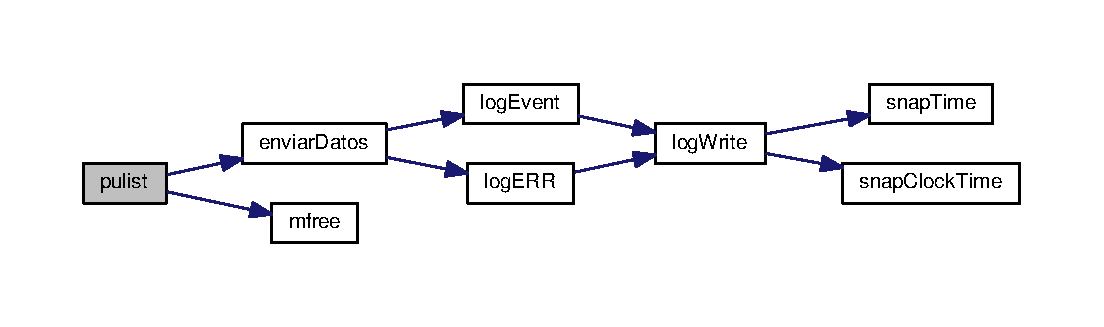
\includegraphics[width=350pt]{user__commands_8h_a2da90a4a7474a7a220ab1588dedd7ef4_cgraph}
\end{center}
\end{figure}


\hypertarget{user__commands_8h_a8e0f94275dfaa1e7bc564d3555b9402e}{\index{user\-\_\-commands.\-h@{user\-\_\-commands.\-h}!pulusers@{pulusers}}
\index{pulusers@{pulusers}!user_commands.h@{user\-\_\-commands.\-h}}
\subsubsection[{pulusers}]{\setlength{\rightskip}{0pt plus 5cm}int pulusers (
\begin{DoxyParamCaption}
\item[{char $\ast$}]{command}
\end{DoxyParamCaption}
)}}\label{user__commands_8h_a8e0f94275dfaa1e7bc564d3555b9402e}


Comando de usuario L\-U\-S\-E\-R\-S Provides Local and Global user information (Such as Current and Maximum user count).
\begin{DoxyItemize}
\item Syntax\-: L\-U\-S\-E\-R\-S \mbox{[}server\mbox{]}. 
\end{DoxyItemize}


\begin{DoxyParams}{Parameters}
{\em command} & cadena introducida por el usuario en el campo de texto \\
\hline
\end{DoxyParams}
\begin{DoxyReturn}{Returns}
O\-K si todo es correcto, E\-R\-R si se produce un error 
\end{DoxyReturn}

\begin{DoxyCode}
531                            \{
532 
533         \textcolor{keywordtype}{char} command\_enviar[\hyperlink{types_8h_ae7e715c270481406658bbd2bafa2897f}{MAXDATA}];
534         \textcolor{keywordtype}{char}* server;
535         \textcolor{keywordtype}{char} lusers[200];
536 
537         g\_print(\textcolor{stringliteral}{"\(\backslash\)t Mensaje recibido en ULUSERS: %s \(\backslash\)n"}, command);
538         IRCUserParse\_Lusers (command, &server);
539 
540         g\_print(\textcolor{stringliteral}{"\(\backslash\)t server: %s \(\backslash\)n"}, server);
541         sprintf(command\_enviar, \textcolor{stringliteral}{"LUSERS %s\(\backslash\)n\(\backslash\)r"}, server );
542         g\_print(\textcolor{stringliteral}{"\(\backslash\)t Mensaje a enviar en ULUSERS: %s \(\backslash\)n"}, command\_enviar);
543 
544         \hyperlink{conexion__tcp_8h_ab9468ce1338cfca5736ab407ba155f55}{enviarDatos}(\hyperlink{aux__functions_8h_acd63fb8dbd9439219e2db08dfc173aa0}{sockfd\_user}, command\_enviar, strlen(command\_enviar));
545         IRCInterface\_PlaneRegisterOutMessage(command\_enviar);
546 
547         strcpy(lusers,\textcolor{stringliteral}{"LUSERS "});
548         strcat(lusers, server);
549         \hyperlink{aux__functions_8h_a040868784608606fad914fea56fc65b8}{IRCInterface\_WriteSystem\_Pretty}(\textcolor{stringliteral}{"*"}, \textcolor{stringliteral}{"------------------------------
      "});
550         \hyperlink{aux__functions_8h_a040868784608606fad914fea56fc65b8}{IRCInterface\_WriteSystem\_Pretty}(\textcolor{stringliteral}{"*"}, lusers);
551         \hyperlink{aux__functions_8h_a2480cc4793bf25a16cc731dc9d033582}{mfree}(1, server);
552         \textcolor{keywordflow}{return} \hyperlink{daemon_8h_aba51915c87d64af47fb1cc59348961c9}{OK};
553 \}
\end{DoxyCode}


Here is the call graph for this function\-:
\nopagebreak
\begin{figure}[H]
\begin{center}
\leavevmode
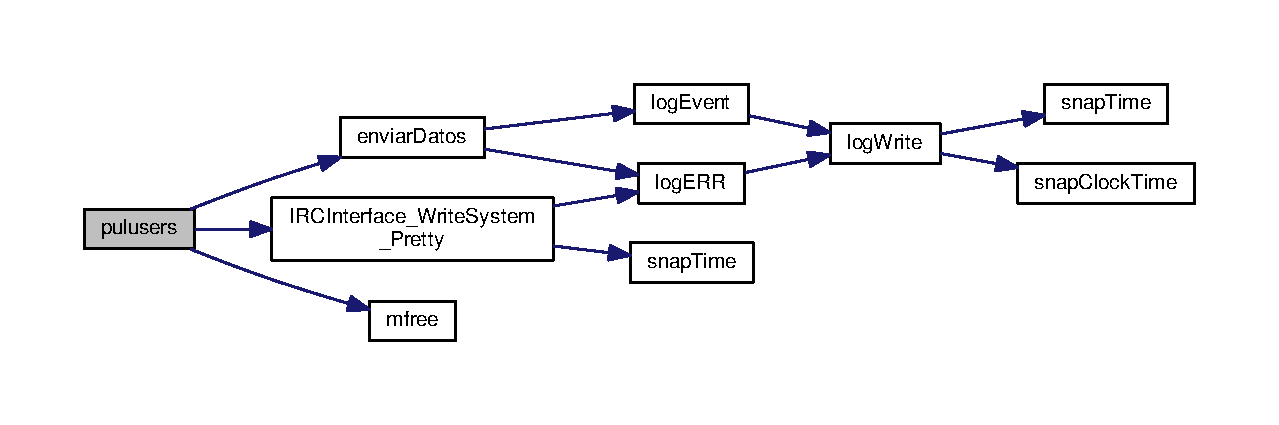
\includegraphics[width=350pt]{user__commands_8h_a8e0f94275dfaa1e7bc564d3555b9402e_cgraph}
\end{center}
\end{figure}


\hypertarget{user__commands_8h_a448b3ec98632740523ee7a20c5bc81dd}{\index{user\-\_\-commands.\-h@{user\-\_\-commands.\-h}!pumode@{pumode}}
\index{pumode@{pumode}!user_commands.h@{user\-\_\-commands.\-h}}
\subsubsection[{pumode}]{\setlength{\rightskip}{0pt plus 5cm}int pumode (
\begin{DoxyParamCaption}
\item[{char $\ast$}]{command}
\end{DoxyParamCaption}
)}}\label{user__commands_8h_a448b3ec98632740523ee7a20c5bc81dd}

\begin{DoxyCode}
27 \{ \textcolor{keywordflow}{return} -1; \} \textcolor{comment}{// ya se envia con los botones}
\end{DoxyCode}
\hypertarget{user__commands_8h_a4d9661d482929bb458b85e70c6170d74}{\index{user\-\_\-commands.\-h@{user\-\_\-commands.\-h}!pumotd@{pumotd}}
\index{pumotd@{pumotd}!user_commands.h@{user\-\_\-commands.\-h}}
\subsubsection[{pumotd}]{\setlength{\rightskip}{0pt plus 5cm}int pumotd (
\begin{DoxyParamCaption}
\item[{char $\ast$}]{command}
\end{DoxyParamCaption}
)}}\label{user__commands_8h_a4d9661d482929bb458b85e70c6170d74}


Comando de usuario M\-O\-T\-D Displays the Message Of The Day of the I\-R\-C Server you are logged onto.
\begin{DoxyItemize}
\item Syntax\-: M\-O\-T\-D M\-O\-T\-D $<$server$>$ 
\end{DoxyItemize}


\begin{DoxyParams}{Parameters}
{\em command} & cadena introducida por el usuario en el campo de texto \\
\hline
\end{DoxyParams}
\begin{DoxyReturn}{Returns}
O\-K si todo es correcto, E\-R\-R si se produce un error 
\end{DoxyReturn}

\begin{DoxyCode}
565                          \{
566 
567         \textcolor{keywordtype}{char} command\_enviar[\hyperlink{types_8h_ae7e715c270481406658bbd2bafa2897f}{MAXDATA}];
568         \textcolor{keywordtype}{char}* server;
569 
570         g\_print(\textcolor{stringliteral}{"\(\backslash\)t Mensaje recibido en UMOTD: %s \(\backslash\)n"}, command);
571         IRCUserParse\_Motd (command, &server);
572         g\_print(\textcolor{stringliteral}{"\(\backslash\)t server: %s \(\backslash\)n"}, server);
573         sprintf(command\_enviar, \textcolor{stringliteral}{"MOTD %s\(\backslash\)n\(\backslash\)r"}, server );
574         g\_print(\textcolor{stringliteral}{"\(\backslash\)t Mensaje a enviar en UMOTD: %s \(\backslash\)n"}, command\_enviar);
575 
576         \hyperlink{conexion__tcp_8h_ab9468ce1338cfca5736ab407ba155f55}{enviarDatos}(\hyperlink{aux__functions_8h_acd63fb8dbd9439219e2db08dfc173aa0}{sockfd\_user}, command\_enviar, strlen(command\_enviar));
577         IRCInterface\_PlaneRegisterOutMessage(command\_enviar);
578         \hyperlink{aux__functions_8h_a2480cc4793bf25a16cc731dc9d033582}{mfree}(1, server);
579         \textcolor{keywordflow}{return} \hyperlink{daemon_8h_aba51915c87d64af47fb1cc59348961c9}{OK};
580 \}
\end{DoxyCode}


Here is the call graph for this function\-:
\nopagebreak
\begin{figure}[H]
\begin{center}
\leavevmode
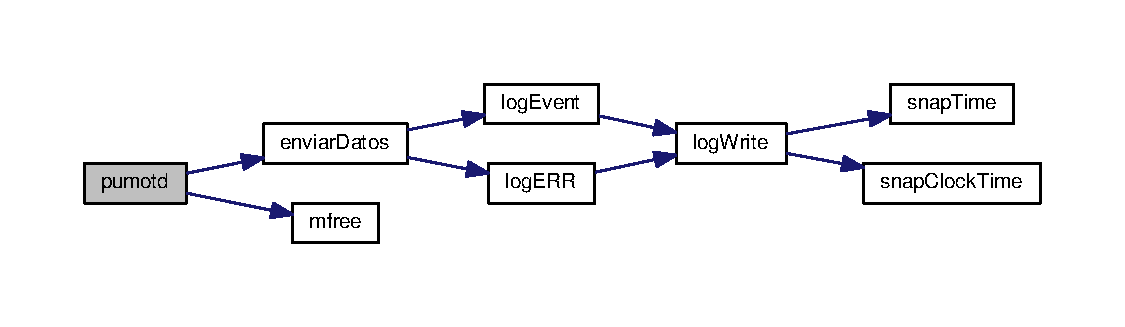
\includegraphics[width=350pt]{user__commands_8h_a4d9661d482929bb458b85e70c6170d74_cgraph}
\end{center}
\end{figure}


\hypertarget{user__commands_8h_a322cdf0baafadcd1784ab6c8f6d48f04}{\index{user\-\_\-commands.\-h@{user\-\_\-commands.\-h}!pumsg@{pumsg}}
\index{pumsg@{pumsg}!user_commands.h@{user\-\_\-commands.\-h}}
\subsubsection[{pumsg}]{\setlength{\rightskip}{0pt plus 5cm}int pumsg (
\begin{DoxyParamCaption}
\item[{char $\ast$}]{command}
\end{DoxyParamCaption}
)}}\label{user__commands_8h_a322cdf0baafadcd1784ab6c8f6d48f04}


Comando de usuario M\-S\-G y P\-R\-I\-V\-M\-S\-G. 


\begin{DoxyParams}{Parameters}
{\em command} & cadena introducida por el usuario en el campo de texto \\
\hline
\end{DoxyParams}
\begin{DoxyReturn}{Returns}
O\-K si todo es correcto, E\-R\-R si se produce un error 
\end{DoxyReturn}

\begin{DoxyCode}
267                         \{
268         \textcolor{keywordtype}{char}* nickorchannel;
269         \textcolor{keywordtype}{char}* msg;
270         \textcolor{keywordtype}{char} *command\_enviar = NULL;
271         \textcolor{keywordtype}{char} *prefix = NULL;
272         \textcolor{keywordtype}{int} ret;
273 
274         \textcolor{comment}{//<< privmsg gomupo :probando}
275         \textcolor{comment}{//>> :gomupo!~gonzalo@119.181.218.87.dynamic.jazztel.es PRIVMSG gomupo :probando}
276         ret = IRCUserParse\_Msg(command, &nickorchannel, &msg);
277         \textcolor{keywordflow}{if}(ret != IRC\_OK)\{
278                 g\_print(\textcolor{stringliteral}{"ERROR - IRCInterface\_NewCommandText - UMSG - IRCUserParse\_Msg\(\backslash\)n"});
279                 \textcolor{keywordflow}{return} \hyperlink{types_8h_a735563036dced0b7d6cc98f97ea4978b}{ERR};
280         \}
281         g\_print(\textcolor{stringliteral}{"\(\backslash\)t command: %s \(\backslash\)n"}, command);
282         g\_print(\textcolor{stringliteral}{"\(\backslash\)t nickorchannel: %s \(\backslash\)n"}, nickorchannel);
283         g\_print(\textcolor{stringliteral}{"\(\backslash\)t msg: %s \(\backslash\)n"}, msg);
284 
285         ret = IRCMsg\_Privmsg (&command\_enviar, prefix, nickorchannel, msg);
286         \textcolor{keywordflow}{if}(ret == \hyperlink{types_8h_a735563036dced0b7d6cc98f97ea4978b}{ERR})\{
287                 g\_print(\textcolor{stringliteral}{"ERROR: IRCInterface\_NewCommandText - IRCMsg\_Privmsg \(\backslash\)n"});
288                 \textcolor{keywordflow}{return} \hyperlink{types_8h_a735563036dced0b7d6cc98f97ea4978b}{ERR};
289         \}
290 
291         g\_print(\textcolor{stringliteral}{"\(\backslash\)t Mensaje a enviar command\_enviar en pumsg: %s \(\backslash\)n"},command\_enviar);
292         ret = \hyperlink{conexion__tcp_8h_ab9468ce1338cfca5736ab407ba155f55}{enviarDatos}(\hyperlink{aux__functions_8h_acd63fb8dbd9439219e2db08dfc173aa0}{sockfd\_user}, command\_enviar, strlen(command\_enviar));
293         \textcolor{keywordflow}{if}(ret == \hyperlink{types_8h_a735563036dced0b7d6cc98f97ea4978b}{ERR})\{
294                 g\_print(\textcolor{stringliteral}{"ERROR: IRCInterface\_NewCommandText - enviarDatos - Names\(\backslash\)n"});
295                 \textcolor{keywordflow}{return} \hyperlink{types_8h_a735563036dced0b7d6cc98f97ea4978b}{ERR};
296         \}
297         IRCInterface\_PlaneRegisterOutMessage(command\_enviar);
298         \textcolor{comment}{//No recibimos nada en este comando, los mensajes de otros usuarios los recibimos por otro hilo}
299         IRCInterface\_WriteChannel (nickorchannel, \hyperlink{user__commands_8h_a7e2f32e47f3780a66e19651d8e79bced}{nick\_user}, msg);
300         \hyperlink{aux__functions_8h_a2480cc4793bf25a16cc731dc9d033582}{mfree}(4, command\_enviar, nickorchannel, prefix, msg);
301         \textcolor{keywordflow}{return} \hyperlink{daemon_8h_aba51915c87d64af47fb1cc59348961c9}{OK};
302 \}
\end{DoxyCode}


Here is the call graph for this function\-:
\nopagebreak
\begin{figure}[H]
\begin{center}
\leavevmode
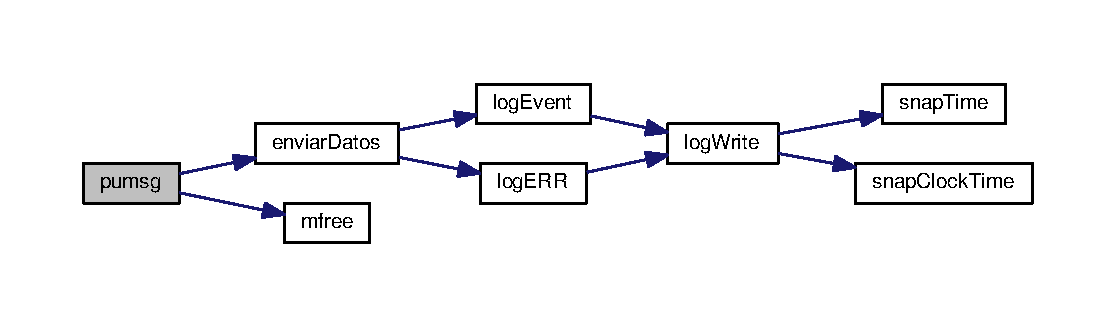
\includegraphics[width=350pt]{user__commands_8h_a322cdf0baafadcd1784ab6c8f6d48f04_cgraph}
\end{center}
\end{figure}


\hypertarget{user__commands_8h_abaae116595df34db33e65e3d9d225103}{\index{user\-\_\-commands.\-h@{user\-\_\-commands.\-h}!punames@{punames}}
\index{punames@{punames}!user_commands.h@{user\-\_\-commands.\-h}}
\subsubsection[{punames}]{\setlength{\rightskip}{0pt plus 5cm}int punames (
\begin{DoxyParamCaption}
\item[{char $\ast$}]{command}
\end{DoxyParamCaption}
)}}\label{user__commands_8h_abaae116595df34db33e65e3d9d225103}


Comando de usuario N\-A\-M\-E\-S. 


\begin{DoxyParams}{Parameters}
{\em command} & cadena introducida por el usuario en el campo de texto \\
\hline
\end{DoxyParams}
\begin{DoxyReturn}{Returns}
O\-K si todo es correcto, E\-R\-R si se produce un error 
\end{DoxyReturn}

\begin{DoxyCode}
64                           \{ 
65         \textcolor{comment}{//<< NAMES #redes2}
66         \textcolor{comment}{//>> :irc.eps.net 353 gomupo = #redes2 :flowey cgs gomupo Mamo\_1 qwerttyue asdfgh alpeh ArcaFacts
       BotGram}
67         \textcolor{keywordtype}{char}* channels;
68         \textcolor{keywordtype}{char}* passwords;
69         \textcolor{keywordtype}{char}* command\_enviar;
70         \textcolor{keywordtype}{char}* prefix = NULL;
71         \textcolor{keywordtype}{char}* target = NULL;
72         \textcolor{keywordtype}{char} channels\_passwords [\hyperlink{types_8h_ae7e715c270481406658bbd2bafa2897f}{MAXDATA}] = \{0\};
73         \textcolor{keywordtype}{int} ret;
74 
75         g\_print(\hyperlink{types_8h_af54a5a977c0c499323d656315f008ee0}{MAG} \textcolor{stringliteral}{"\(\backslash\)n<< [user command] NOTICE - command = %s\(\backslash\)n"} \hyperlink{types_8h_ab702106cf3b3e96750b6845ded4e0299}{RESET}, command);
76         \textcolor{comment}{/*Comprobar si es un comando names sin argumentos, en caso afirmativo no utilizar la función de
       Eloy ya que}
77 \textcolor{comment}{        parece que falla, y mandarlo tal cual*/}
78         \textcolor{comment}{//Usamos strcasecmp para que den igual minusculas}
79         \textcolor{keywordflow}{if}((0 == strcasecmp(command,\textcolor{stringliteral}{"/names"})) && (strlen(command) == strlen(\textcolor{stringliteral}{"/names"})))\{
80                 g\_print(\textcolor{stringliteral}{"\(\backslash\)t Command names sin argumentos: %s \(\backslash\)n"},command);
81                 ret = IRCMsg\_Names (&command\_enviar, prefix, channels\_passwords, target);
82                 \textcolor{keywordflow}{if}(ret != IRC\_OK)\{
83                         g\_print(\hyperlink{types_8h_a8d23feea868a983c8c2b661e1e16972f}{RED} \textcolor{stringliteral}{"ERROR - In punames: IRCMsg\_Names no devolvio IRC\_OK\(\backslash\)n"} 
      \hyperlink{types_8h_ab702106cf3b3e96750b6845ded4e0299}{RESET});
84                         \textcolor{keywordflow}{return} \hyperlink{types_8h_a735563036dced0b7d6cc98f97ea4978b}{ERR};
85                 \}
86                 g\_print(\textcolor{stringliteral}{"\(\backslash\)t command\_enviar names sin argumentos: %s \(\backslash\)n"},command\_enviar);
87                 ret = \hyperlink{conexion__tcp_8h_ab9468ce1338cfca5736ab407ba155f55}{enviarDatos}(\hyperlink{aux__functions_8h_acd63fb8dbd9439219e2db08dfc173aa0}{sockfd\_user},command\_enviar, strlen(command\_enviar))
      ;
88                 \textcolor{keywordflow}{if}(ret == \hyperlink{types_8h_a735563036dced0b7d6cc98f97ea4978b}{ERR})\{
89                         g\_print(\hyperlink{types_8h_a8d23feea868a983c8c2b661e1e16972f}{RED} \textcolor{stringliteral}{"ERROR - In punames: enviarDatos() devolvio error (ver .log)\(\backslash\)n\(\backslash\)t\(\backslash\)tEl
       cliente se cerrará.\(\backslash\)n"} \hyperlink{types_8h_ab702106cf3b3e96750b6845ded4e0299}{RESET});
90                         exit(1);
91                 \}
92                 \textcolor{keywordflow}{if}(ret == 0)\{ \textcolor{comment}{//timeout seguramente}
93                         g\_print(\hyperlink{types_8h_a8d23feea868a983c8c2b661e1e16972f}{RED} \textcolor{stringliteral}{"ERROR - In punames: enviarDatos() mandó 0 Bytes(ver .log)\(\backslash\)n\(\backslash\)t\(\backslash\)t
      (Timeout)El cliente se cerrará.\(\backslash\)n"} \hyperlink{types_8h_ab702106cf3b3e96750b6845ded4e0299}{RESET});
94                         exit(1);
95                 \}
96                 IRCInterface\_PlaneRegisterOutMessage(command);
97                 free(command\_enviar);
98                 \textcolor{keywordflow}{return} \hyperlink{daemon_8h_aba51915c87d64af47fb1cc59348961c9}{OK};
99         \}
100 
101         ret = IRCUserParse\_Names(command, &channels, &passwords);
102         \textcolor{keywordflow}{if}(ret != IRC\_OK)\{
103                 g\_print(\hyperlink{types_8h_a8d23feea868a983c8c2b661e1e16972f}{RED} \textcolor{stringliteral}{"ERROR - In punames: IRCUserParse\_Names no devolvio IRC\_OK\(\backslash\)n"} 
      \hyperlink{types_8h_ab702106cf3b3e96750b6845ded4e0299}{RESET});
104                 \textcolor{keywordflow}{return} \hyperlink{types_8h_a735563036dced0b7d6cc98f97ea4978b}{ERR};
105         \}
106         g\_print(\textcolor{stringliteral}{"\(\backslash\)t command: %s \(\backslash\)n"},command);
107         g\_print(\textcolor{stringliteral}{"\(\backslash\)t channels : %s \(\backslash\)n"},channels);
108         g\_print(\textcolor{stringliteral}{"\(\backslash\)t passwords : %s \(\backslash\)n"},passwords);
109 
110         sprintf(channels\_passwords,\textcolor{stringliteral}{"%s %s"},channels,passwords?passwords:\textcolor{stringliteral}{""});
111 
112         ret = IRCMsg\_Names (&command\_enviar, prefix, channels\_passwords, target);
113         \textcolor{keywordflow}{if}(ret != IRC\_OK)\{
114                 g\_print(\hyperlink{types_8h_a8d23feea868a983c8c2b661e1e16972f}{RED} \textcolor{stringliteral}{"ERROR - In punames: IRCMsg\_Names no devolvio IRC\_OK\(\backslash\)n"} 
      \hyperlink{types_8h_ab702106cf3b3e96750b6845ded4e0299}{RESET});
115                 \textcolor{keywordflow}{return} \hyperlink{types_8h_a735563036dced0b7d6cc98f97ea4978b}{ERR};
116         \}
117         g\_print(\textcolor{stringliteral}{"\(\backslash\)t Mensaje a enviar command\_enviar: %s \(\backslash\)n"},command\_enviar);
118 
119         \hyperlink{conexion__tcp_8h_ab9468ce1338cfca5736ab407ba155f55}{enviarDatos}(\hyperlink{aux__functions_8h_acd63fb8dbd9439219e2db08dfc173aa0}{sockfd\_user}, command\_enviar, strlen(command\_enviar));
120 
121         IRCInterface\_PlaneRegisterOutMessage(command\_enviar);
122         \hyperlink{aux__functions_8h_a2480cc4793bf25a16cc731dc9d033582}{mfree}(5, command\_enviar, channels, passwords, prefix, target);
123         \textcolor{keywordflow}{return} \hyperlink{daemon_8h_aba51915c87d64af47fb1cc59348961c9}{OK};
124 \}
\end{DoxyCode}


Here is the call graph for this function\-:
\nopagebreak
\begin{figure}[H]
\begin{center}
\leavevmode
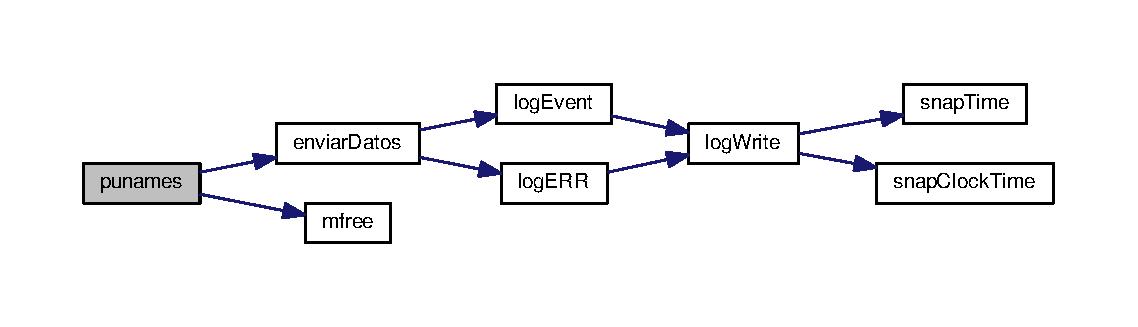
\includegraphics[width=350pt]{user__commands_8h_abaae116595df34db33e65e3d9d225103_cgraph}
\end{center}
\end{figure}


\hypertarget{user__commands_8h_a93cab9103f7f4815ff20b47dcf0c117c}{\index{user\-\_\-commands.\-h@{user\-\_\-commands.\-h}!punick@{punick}}
\index{punick@{punick}!user_commands.h@{user\-\_\-commands.\-h}}
\subsubsection[{punick}]{\setlength{\rightskip}{0pt plus 5cm}int punick (
\begin{DoxyParamCaption}
\item[{char $\ast$}]{command}
\end{DoxyParamCaption}
)}}\label{user__commands_8h_a93cab9103f7f4815ff20b47dcf0c117c}


Comando de usuario N\-I\-C\-K Changes your \char`\"{}\-Online Identity\char`\"{} on a server. All those in the channel you are in will be alerted of your nickname change.
\begin{DoxyItemize}
\item Syntax\-: N\-I\-C\-K $<$new nickname$>$=\char`\"{}\char`\"{}$>$ 
\end{DoxyItemize}


\begin{DoxyParams}{Parameters}
{\em command} & cadena introducida por el usuario en el campo de texto \\
\hline
\end{DoxyParams}
\begin{DoxyReturn}{Returns}
O\-K si todo es correcto, E\-R\-R si se produce un error 
\end{DoxyReturn}

\begin{DoxyCode}
444                          \{
445 
446         \textcolor{keywordtype}{char}* command\_enviar;
447         \textcolor{keywordtype}{char} *newnick;
448 
449         IRCUserParse\_Nick (command, &newnick);
450         IRCMsg\_Nick (&command\_enviar, NULL, newnick, NULL);
451         g\_print(\textcolor{stringliteral}{"\(\backslash\)t Mensaje a enviar command\_enviar en NICK: %s \(\backslash\)n"},command\_enviar);
452 
453         \hyperlink{conexion__tcp_8h_ab9468ce1338cfca5736ab407ba155f55}{enviarDatos}(\hyperlink{aux__functions_8h_acd63fb8dbd9439219e2db08dfc173aa0}{sockfd\_user}, command\_enviar, strlen(command\_enviar));
454         IRCInterface\_PlaneRegisterOutMessage(command\_enviar);
455         \hyperlink{aux__functions_8h_a2480cc4793bf25a16cc731dc9d033582}{mfree}(2, command\_enviar, newnick);
456         \textcolor{keywordflow}{return} \hyperlink{daemon_8h_aba51915c87d64af47fb1cc59348961c9}{OK};
457 \}
\end{DoxyCode}


Here is the call graph for this function\-:
\nopagebreak
\begin{figure}[H]
\begin{center}
\leavevmode
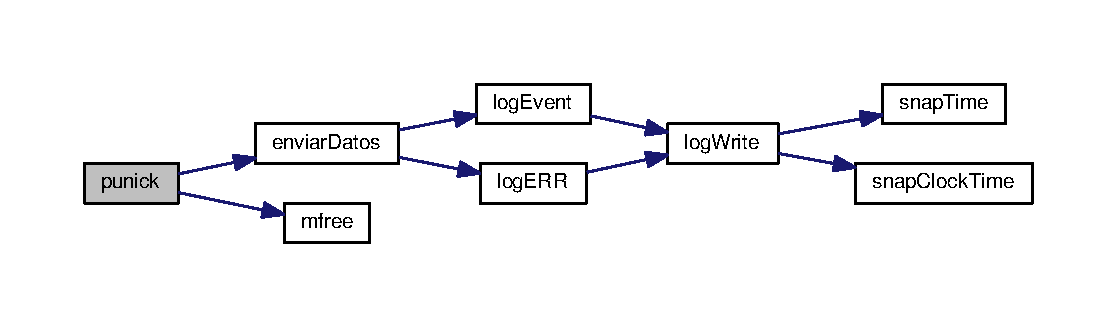
\includegraphics[width=350pt]{user__commands_8h_a93cab9103f7f4815ff20b47dcf0c117c_cgraph}
\end{center}
\end{figure}


\hypertarget{user__commands_8h_a4dd6e13bec86782e1c29bc67c6040b95}{\index{user\-\_\-commands.\-h@{user\-\_\-commands.\-h}!punotice@{punotice}}
\index{punotice@{punotice}!user_commands.h@{user\-\_\-commands.\-h}}
\subsubsection[{punotice}]{\setlength{\rightskip}{0pt plus 5cm}int punotice (
\begin{DoxyParamCaption}
\item[{char $\ast$}]{command}
\end{DoxyParamCaption}
)}}\label{user__commands_8h_a4dd6e13bec86782e1c29bc67c6040b95}


Comando de usuario N\-O\-T\-I\-C\-E Send a notice to a user, channel or server.
\begin{DoxyItemize}
\item N\-O\-T\-I\-C\-E $<$nick$>$ $<$text$>$ Send a notice to a user. Ex\-: /\-N\-O\-T\-I\-C\-E Blah hi, how are you?
\item N\-O\-T\-I\-C\-E $<$\#channel$>$ $<$text$>$ Send a notice to a channel. Ex\-: /\-N\-O\-T\-I\-C\-E \#room Hi all, this is annoying. 
\end{DoxyItemize}


\begin{DoxyParams}{Parameters}
{\em command} & cadena introducida por el usuario en el campo de texto \\
\hline
\end{DoxyParams}
\begin{DoxyReturn}{Returns}
O\-K si todo es correcto, E\-R\-R si se produce un error 
\end{DoxyReturn}

\begin{DoxyCode}
597                            \{
598 
599         \textcolor{keywordtype}{char} *command\_enviar, mensaje[\hyperlink{types_8h_ae7e715c270481406658bbd2bafa2897f}{MAXDATA}];
600         \textcolor{keywordtype}{char}* target, *msg;
601 
602         g\_print(\textcolor{stringliteral}{"\(\backslash\)t Mensaje recibido en UNOTICE: %s \(\backslash\)n"}, command);
603         IRCUserParse\_Notice (command, &target, &msg);
604 
605         IRCMsg\_Notice (&command\_enviar, NULL, target, msg);
606 
607         g\_print(\textcolor{stringliteral}{"\(\backslash\)t Mensaje a enviar en UNOTICE: %s \(\backslash\)n"}, command\_enviar);
608         \hyperlink{conexion__tcp_8h_ab9468ce1338cfca5736ab407ba155f55}{enviarDatos}(\hyperlink{aux__functions_8h_acd63fb8dbd9439219e2db08dfc173aa0}{sockfd\_user}, command\_enviar, strlen(command\_enviar));
609         IRCInterface\_PlaneRegisterOutMessage(command\_enviar);
610 
611         \textcolor{keywordflow}{if}(target[0] == \textcolor{charliteral}{'#'})\{
612                 sprintf(mensaje, \textcolor{stringliteral}{">%s/%s<"}, \hyperlink{user__commands_8h_a7e2f32e47f3780a66e19651d8e79bced}{nick\_user}, target);
613                 IRCInterface\_WriteChannel (target, mensaje, msg);
614         \} \textcolor{keywordflow}{else} \{
615                 sprintf(mensaje, \textcolor{stringliteral}{">%s<"}, \hyperlink{user__commands_8h_a7e2f32e47f3780a66e19651d8e79bced}{nick\_user});           
616                 IRCInterface\_AddNewChannel (target, 0);
617                 IRCInterface\_WriteChannel (target, mensaje, msg);
618         \}
619         \hyperlink{aux__functions_8h_a2480cc4793bf25a16cc731dc9d033582}{mfree}(3, command\_enviar, target, msg);
620         \textcolor{keywordflow}{return} \hyperlink{daemon_8h_aba51915c87d64af47fb1cc59348961c9}{OK};
621 \}
\end{DoxyCode}


Here is the call graph for this function\-:
\nopagebreak
\begin{figure}[H]
\begin{center}
\leavevmode
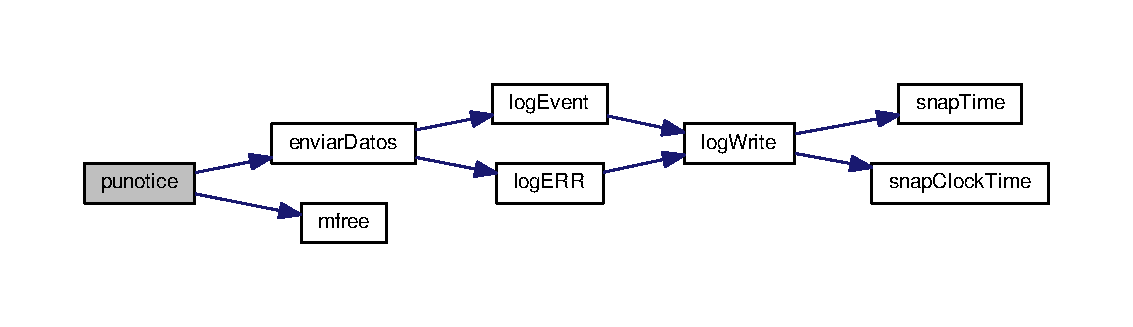
\includegraphics[width=350pt]{user__commands_8h_a4dd6e13bec86782e1c29bc67c6040b95_cgraph}
\end{center}
\end{figure}


\hypertarget{user__commands_8h_ab51cd004b9746694fb19829952779c6b}{\index{user\-\_\-commands.\-h@{user\-\_\-commands.\-h}!puoper@{puoper}}
\index{puoper@{puoper}!user_commands.h@{user\-\_\-commands.\-h}}
\subsubsection[{puoper}]{\setlength{\rightskip}{0pt plus 5cm}int puoper (
\begin{DoxyParamCaption}
\item[{char $\ast$}]{command}
\end{DoxyParamCaption}
)}}\label{user__commands_8h_ab51cd004b9746694fb19829952779c6b}

\begin{DoxyCode}
31 \{ \textcolor{keywordflow}{return} -1; \}
\end{DoxyCode}
\hypertarget{user__commands_8h_adc5c5d5b72106761066833022c9bc83d}{\index{user\-\_\-commands.\-h@{user\-\_\-commands.\-h}!pupart@{pupart}}
\index{pupart@{pupart}!user_commands.h@{user\-\_\-commands.\-h}}
\subsubsection[{pupart}]{\setlength{\rightskip}{0pt plus 5cm}int pupart (
\begin{DoxyParamCaption}
\item[{char $\ast$}]{command}
\end{DoxyParamCaption}
)}}\label{user__commands_8h_adc5c5d5b72106761066833022c9bc83d}


Comando de usuario P\-A\-R\-T Used to part (or leave) a channel you currently occupy. All those in the channel will be notified of your departure. If you specify a reason it will be displayed to the users on the channel
\begin{DoxyItemize}
\item Syntax\-: P\-A\-R\-T $<$chan$>$,$<$chan2$>$,$<$chan3$>$,$<$chan4$>$ $<$reason$>$ 
\end{DoxyItemize}


\begin{DoxyParams}{Parameters}
{\em command} & cadena introducida por el usuario en el campo de texto \\
\hline
\end{DoxyParams}
\begin{DoxyReturn}{Returns}
O\-K si todo es correcto, E\-R\-R si se produce un error 
\end{DoxyReturn}

\begin{DoxyCode}
386                          \{
387         \textcolor{keywordtype}{char}* channel;
388         \textcolor{keywordtype}{char} command\_enviar[\hyperlink{types_8h_ae7e715c270481406658bbd2bafa2897f}{MAXDATA}];
389 
390         IRCUserParse\_Part(command, &channel);
391         sprintf(command\_enviar, \textcolor{stringliteral}{"PART %s :Saliendo\(\backslash\)r\(\backslash\)n"}, channel?channel:IRCInterface\_ActiveChannelName());
392 
393         \hyperlink{conexion__tcp_8h_ab9468ce1338cfca5736ab407ba155f55}{enviarDatos}(\hyperlink{aux__functions_8h_acd63fb8dbd9439219e2db08dfc173aa0}{sockfd\_user}, command\_enviar, strlen(command\_enviar));
394         IRCInterface\_PlaneRegisterOutMessage(command\_enviar);
395         \hyperlink{aux__functions_8h_a2480cc4793bf25a16cc731dc9d033582}{mfree}(1, channel);
396         \textcolor{keywordflow}{return} \hyperlink{daemon_8h_aba51915c87d64af47fb1cc59348961c9}{OK};
397 \}
\end{DoxyCode}


Here is the call graph for this function\-:
\nopagebreak
\begin{figure}[H]
\begin{center}
\leavevmode
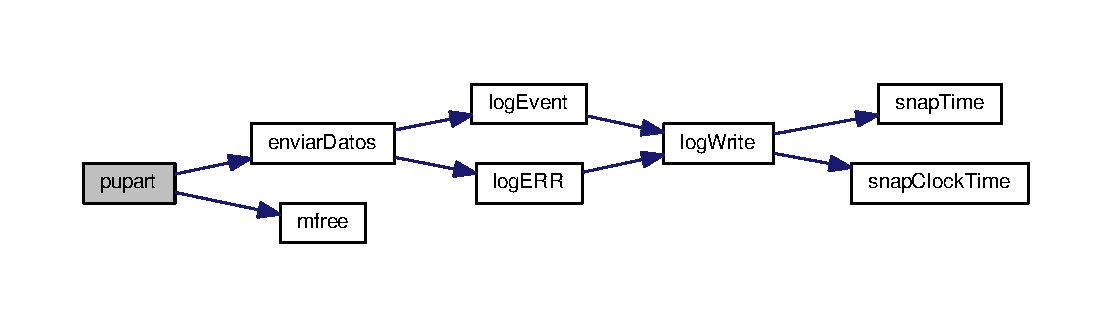
\includegraphics[width=350pt]{user__commands_8h_adc5c5d5b72106761066833022c9bc83d_cgraph}
\end{center}
\end{figure}


\hypertarget{user__commands_8h_a1af5de7d9cb449f78a7f511d28c64ba9}{\index{user\-\_\-commands.\-h@{user\-\_\-commands.\-h}!pupartall@{pupartall}}
\index{pupartall@{pupartall}!user_commands.h@{user\-\_\-commands.\-h}}
\subsubsection[{pupartall}]{\setlength{\rightskip}{0pt plus 5cm}int pupartall (
\begin{DoxyParamCaption}
\item[{char $\ast$}]{command}
\end{DoxyParamCaption}
)}}\label{user__commands_8h_a1af5de7d9cb449f78a7f511d28c64ba9}

\begin{DoxyCode}
28 \{ \textcolor{keywordflow}{return} -1; \}
\end{DoxyCode}
\hypertarget{user__commands_8h_a8149f7beb37fd789f142acb2113efd1c}{\index{user\-\_\-commands.\-h@{user\-\_\-commands.\-h}!puquery@{puquery}}
\index{puquery@{puquery}!user_commands.h@{user\-\_\-commands.\-h}}
\subsubsection[{puquery}]{\setlength{\rightskip}{0pt plus 5cm}int puquery (
\begin{DoxyParamCaption}
\item[{char $\ast$}]{command}
\end{DoxyParamCaption}
)}}\label{user__commands_8h_a8149f7beb37fd789f142acb2113efd1c}


Comando de usuario Q\-U\-E\-R\-Y Use the \char`\"{}/query $<$user$>$\char`\"{} command to specify that every message you type should be directed to a single user. 


\begin{DoxyParams}{Parameters}
{\em command} & cadena introducida por el usuario en el campo de texto \\
\hline
\end{DoxyParams}
\begin{DoxyReturn}{Returns}
O\-K si todo es correcto, E\-R\-R si se produce un error 
\end{DoxyReturn}

\begin{DoxyCode}
661                           \{
662 
663         \textcolor{keywordtype}{char}* nickorchannel, *msg;
664 
665         IRCUserParse\_Query (command, &nickorchannel, &msg);
666         g\_print(\textcolor{stringliteral}{"\(\backslash\)t Mensaje recibido en UQUERY: %s \(\backslash\)n"}, command);
667         g\_print(\textcolor{stringliteral}{"\(\backslash\)t nickorchannel: %s \(\backslash\)n"}, nickorchannel);
668         g\_print(\textcolor{stringliteral}{"\(\backslash\)t msg: %s \(\backslash\)n"}, msg);
669 
670         \textcolor{keywordflow}{if}(nickorchannel != NULL)\{
671                 IRCInterface\_AddNewChannel (nickorchannel, 0);
672         \}
673         \hyperlink{aux__functions_8h_a2480cc4793bf25a16cc731dc9d033582}{mfree}(2, nickorchannel, msg);
674     \textcolor{keywordflow}{return} \hyperlink{daemon_8h_aba51915c87d64af47fb1cc59348961c9}{OK};
675 \}\end{DoxyCode}


Here is the call graph for this function\-:
\nopagebreak
\begin{figure}[H]
\begin{center}
\leavevmode
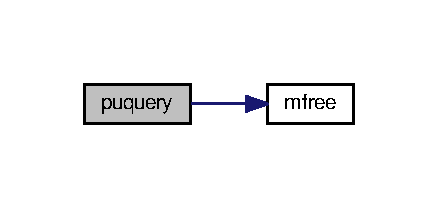
\includegraphics[width=210pt]{user__commands_8h_a8149f7beb37fd789f142acb2113efd1c_cgraph}
\end{center}
\end{figure}


\hypertarget{user__commands_8h_ad738a7d361fe18d7774bab370a4454a8}{\index{user\-\_\-commands.\-h@{user\-\_\-commands.\-h}!puquit@{puquit}}
\index{puquit@{puquit}!user_commands.h@{user\-\_\-commands.\-h}}
\subsubsection[{puquit}]{\setlength{\rightskip}{0pt plus 5cm}int puquit (
\begin{DoxyParamCaption}
\item[{char $\ast$}]{command}
\end{DoxyParamCaption}
)}}\label{user__commands_8h_ad738a7d361fe18d7774bab370a4454a8}


Comando de usuario Q\-U\-I\-T En principio solo se llama con\-: 


\begin{DoxyItemize}
\item Callback\-: Boton 'Desconectar' -\/$>$ \hyperlink{xchat2_8c_a8bf0424ef7f845be79a056e9aed56fe2}{I\-R\-C\-Interface\-\_\-\-Disconnect\-Server(char $\ast$server, int port)}
\item Callback\-: '/\-Q\-U\-I\-T en chat + E\-N\-T\-E\-R' -\/$>$ I\-R\-C\-Interface\-\_\-\-New\-Command\-Text(\char`\"{}/\-Q\-U\-I\-T \char`\"{}) 
\begin{DoxyParams}{Parameters}
{\em command} & cadena introducida por el usuario en el campo de texto \\
\hline
\end{DoxyParams}
\begin{DoxyReturn}{Returns}
O\-K si todo es correcto, E\-R\-R si se produce un error 
\end{DoxyReturn}

\end{DoxyItemize}
\begin{DoxyCode}
188                          \{
189 
190         \textcolor{keywordtype}{char}* command\_enviar;
191         \textcolor{keywordtype}{char}* reason;
192         \textcolor{comment}{//char command[] = "QUIT :Leaving";}
193 
194         \textcolor{keywordtype}{char}** channelsQuit;
195         \textcolor{keywordtype}{int} numChannelsQuit;
196         \textcolor{keywordtype}{int} i, ret;
197 
198         \textcolor{comment}{//kill hilo 'receive\_messages()'}
199         ret = pthread\_cancel(\hyperlink{user__commands_8h_ab5efd1efa144e252f4c5312ae57bea2e}{recv\_tid});
200         \textcolor{keywordflow}{if} (ret != 0)\{
201                 g\_print(\hyperlink{types_8h_af54a5a977c0c499323d656315f008ee0}{MAG} \textcolor{stringliteral}{"\(\backslash\)npthread\_cancel() return = %d\(\backslash\)n"} \hyperlink{types_8h_ab702106cf3b3e96750b6845ded4e0299}{RESET}, ret);
202         \}
203 
204         IRCUserParse\_Quit (command, &reason);
205         IRCMsg\_Quit (&command\_enviar, NULL, reason ? reason : \textcolor{stringliteral}{"Desconectando..."});
206         g\_print(\textcolor{stringliteral}{"\(\backslash\)t Mensaje a enviar command\_enviar en QUIT: %s \(\backslash\)n"},command\_enviar);
207         \hyperlink{conexion__tcp_8h_ab9468ce1338cfca5736ab407ba155f55}{enviarDatos}(\hyperlink{aux__functions_8h_acd63fb8dbd9439219e2db08dfc173aa0}{sockfd\_user}, command\_enviar, strlen(command\_enviar));
208         IRCInterface\_PlaneRegisterOutMessage(command\_enviar);
209         \hyperlink{conexion__tcp_8h_a831321f466f7f9fa60b0f940b7c2d7da}{cerrarConexion}(\hyperlink{aux__functions_8h_acd63fb8dbd9439219e2db08dfc173aa0}{sockfd\_user}, NULL);
210         \hyperlink{aux__functions_8h_a2480cc4793bf25a16cc731dc9d033582}{mfree}(2, command\_enviar, reason);
211 
212         \textcolor{comment}{/*IRCInterface\_RemoveAllChannels da segmentation fault por alguna razón*/}
213         IRCInterface\_ListAllChannels(&channelsQuit, &numChannelsQuit);
214         \textcolor{keywordflow}{for}(i = 0; i<numChannelsQuit; i++)\{
215                 \textcolor{comment}{//IRCInterface\_WriteChannelThread(channelsQuit[i],"*", "Desconectado.");}
216                 IRCInterface\_RemoveChannel(channelsQuit[i]);
217         \}
218         \hyperlink{aux__functions_8h_a040868784608606fad914fea56fc65b8}{IRCInterface\_WriteSystem\_Pretty}(\textcolor{stringliteral}{"*"}, \textcolor{stringliteral}{"Desconectado."});
219 
220         \textcolor{keywordflow}{return} \hyperlink{daemon_8h_aba51915c87d64af47fb1cc59348961c9}{OK};
221 \}
\end{DoxyCode}


Here is the call graph for this function\-:
\nopagebreak
\begin{figure}[H]
\begin{center}
\leavevmode
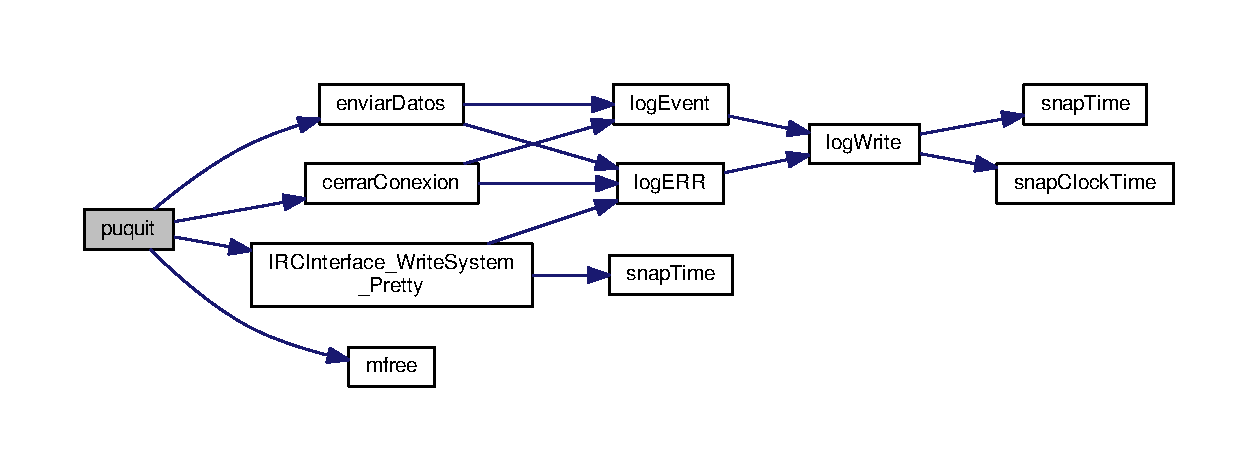
\includegraphics[width=350pt]{user__commands_8h_ad738a7d361fe18d7774bab370a4454a8_cgraph}
\end{center}
\end{figure}


\hypertarget{user__commands_8h_a0a15138d8927dd543805edcc035b8132}{\index{user\-\_\-commands.\-h@{user\-\_\-commands.\-h}!putopic@{putopic}}
\index{putopic@{putopic}!user_commands.h@{user\-\_\-commands.\-h}}
\subsubsection[{putopic}]{\setlength{\rightskip}{0pt plus 5cm}int putopic (
\begin{DoxyParamCaption}
\item[{char $\ast$}]{command}
\end{DoxyParamCaption}
)}}\label{user__commands_8h_a0a15138d8927dd543805edcc035b8132}

\begin{DoxyCode}
36 \{ \textcolor{keywordflow}{return} -1; \} \textcolor{comment}{// se envia con la barra de topic}
\end{DoxyCode}
\hypertarget{user__commands_8h_a8a3e6d36d02bc24a451f806de272c691}{\index{user\-\_\-commands.\-h@{user\-\_\-commands.\-h}!puunaway@{puunaway}}
\index{puunaway@{puunaway}!user_commands.h@{user\-\_\-commands.\-h}}
\subsubsection[{puunaway}]{\setlength{\rightskip}{0pt plus 5cm}int puunaway (
\begin{DoxyParamCaption}
\item[{char $\ast$}]{command}
\end{DoxyParamCaption}
)}}\label{user__commands_8h_a8a3e6d36d02bc24a451f806de272c691}

\begin{DoxyCode}
30 \{ \textcolor{keywordflow}{return} -1; \} \textcolor{comment}{//existe UNAWAY??}
\end{DoxyCode}
\hypertarget{user__commands_8h_aef4e57bf112f9c4a2d51b1a314df0b63}{\index{user\-\_\-commands.\-h@{user\-\_\-commands.\-h}!puwho@{puwho}}
\index{puwho@{puwho}!user_commands.h@{user\-\_\-commands.\-h}}
\subsubsection[{puwho}]{\setlength{\rightskip}{0pt plus 5cm}int puwho (
\begin{DoxyParamCaption}
\item[{char $\ast$}]{command}
\end{DoxyParamCaption}
)}}\label{user__commands_8h_aef4e57bf112f9c4a2d51b1a314df0b63}


Comando de usuario W\-H\-O. 


\begin{DoxyParams}{Parameters}
{\em command} & cadena introducida por el usuario en el campo de texto \\
\hline
\end{DoxyParams}
\begin{DoxyReturn}{Returns}
O\-K si todo es correcto, E\-R\-R si se produce un error 
\end{DoxyReturn}

\begin{DoxyCode}
228                         \{
229 
230         \textcolor{keywordtype}{long} ret = -1;
231 
232         \textcolor{keywordtype}{char}* command\_enviar=NULL;
233         \textcolor{keywordtype}{char}* prefix = NULL;
234         \textcolor{keywordtype}{char}* mask;
235         
236         ret = IRCUserParse\_Who (command, &mask);
237         \textcolor{keywordflow}{if}(ret != IRC\_OK)\{
238                 g\_print(\textcolor{stringliteral}{"ERROR - IRCInterface\_NewCommandText - UWHO - IRCUserParse\_Who"});
239                 \textcolor{keywordflow}{return} -1;
240         \}
241         g\_print(\textcolor{stringliteral}{"\(\backslash\)t command: %s \(\backslash\)n"},command);
242         g\_print(\textcolor{stringliteral}{"\(\backslash\)t mask who: %s \(\backslash\)n"},mask);
243         
244         ret = IRCMsg\_Who (&command\_enviar, prefix, mask, NULL);
245         \textcolor{keywordflow}{if}(ret != IRC\_OK)\{
246                 g\_print(\hyperlink{types_8h_a8d23feea868a983c8c2b661e1e16972f}{RED} \textcolor{stringliteral}{"ERROR - puwho - IRCMsg\_Who \(\backslash\)n"} \hyperlink{types_8h_ab702106cf3b3e96750b6845ded4e0299}{RESET});
247                 \textcolor{keywordflow}{return} \hyperlink{types_8h_a735563036dced0b7d6cc98f97ea4978b}{ERR};
248         \}
249 
250         g\_print(\textcolor{stringliteral}{"\(\backslash\)t command\_enviar: %s \(\backslash\)n"},command\_enviar);
251 
252         \textcolor{keywordflow}{if}(\hyperlink{conexion__tcp_8h_ab9468ce1338cfca5736ab407ba155f55}{enviarDatos}(\hyperlink{aux__functions_8h_acd63fb8dbd9439219e2db08dfc173aa0}{sockfd\_user},command\_enviar, strlen(command\_enviar) == 
      \hyperlink{types_8h_a735563036dced0b7d6cc98f97ea4978b}{ERR}))\{
253                 g\_print(\textcolor{stringliteral}{"ERROR: IRCInterface\_NewCommandText - enviarDatos - Who\(\backslash\)n"});
254                 \textcolor{keywordflow}{return} \hyperlink{types_8h_a735563036dced0b7d6cc98f97ea4978b}{ERR};
255         \}
256 
257         IRCInterface\_PlaneRegisterOutMessage(command\_enviar);   
258         \hyperlink{aux__functions_8h_a2480cc4793bf25a16cc731dc9d033582}{mfree}(3, command\_enviar, prefix, mask);
259         \textcolor{keywordflow}{return} \hyperlink{daemon_8h_aba51915c87d64af47fb1cc59348961c9}{OK};
260 \}
\end{DoxyCode}


Here is the call graph for this function\-:
\nopagebreak
\begin{figure}[H]
\begin{center}
\leavevmode
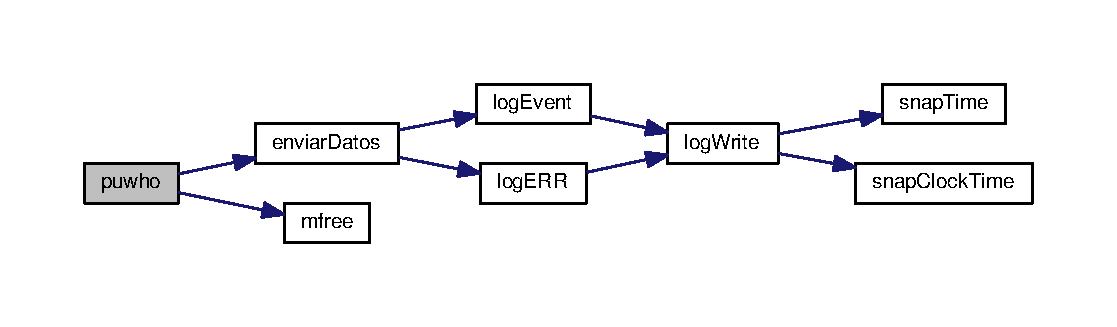
\includegraphics[width=350pt]{user__commands_8h_aef4e57bf112f9c4a2d51b1a314df0b63_cgraph}
\end{center}
\end{figure}


\hypertarget{user__commands_8h_a08bd5900f288bfb5712d3f5ca6e624b6}{\index{user\-\_\-commands.\-h@{user\-\_\-commands.\-h}!puwhois@{puwhois}}
\index{puwhois@{puwhois}!user_commands.h@{user\-\_\-commands.\-h}}
\subsubsection[{puwhois}]{\setlength{\rightskip}{0pt plus 5cm}int puwhois (
\begin{DoxyParamCaption}
\item[{char $\ast$}]{command}
\end{DoxyParamCaption}
)}}\label{user__commands_8h_a08bd5900f288bfb5712d3f5ca6e624b6}


Comando de usuario W\-H\-O\-I\-S Shows information about the user in question, such as their \char`\"{}\-Name\char`\"{}, channels they are currently in, their hostmask, etc.
\begin{DoxyItemize}
\item Syntax\-: W\-H\-O\-I\-S $<$user$>$ 
\end{DoxyItemize}


\begin{DoxyParams}{Parameters}
{\em command} & cadena introducida por el usuario en el campo de texto \\
\hline
\end{DoxyParams}
\begin{DoxyReturn}{Returns}
O\-K si todo es correcto, E\-R\-R si se produce un error 
\end{DoxyReturn}

\begin{DoxyCode}
499                           \{
500 
501         \textcolor{keywordtype}{char} command\_enviar[\hyperlink{types_8h_ae7e715c270481406658bbd2bafa2897f}{MAXDATA}];
502         \textcolor{keywordtype}{char}* nick = NULL;
503         \textcolor{keywordtype}{char} whois[200];
504 
505         g\_print(\textcolor{stringliteral}{"\(\backslash\)t Mensaje recibido en UWHOIS: %s \(\backslash\)n"}, command);
506         IRCUserParse\_Whois (command, &nick);
507 
508         g\_print(\textcolor{stringliteral}{"\(\backslash\)t nick: %s \(\backslash\)n"}, nick);
509         sprintf(command\_enviar, \textcolor{stringliteral}{"WHOIS %s\(\backslash\)n\(\backslash\)r"}, nick );
510         g\_print(\textcolor{stringliteral}{"\(\backslash\)t Mensaje a enviar en UWHOIS: %s \(\backslash\)n"}, command\_enviar);
511 
512         \hyperlink{conexion__tcp_8h_ab9468ce1338cfca5736ab407ba155f55}{enviarDatos}(\hyperlink{aux__functions_8h_acd63fb8dbd9439219e2db08dfc173aa0}{sockfd\_user}, command\_enviar, strlen(command\_enviar));
513         IRCInterface\_PlaneRegisterOutMessage(command\_enviar);
514 
515         strcpy(whois,\textcolor{stringliteral}{"WHOIS "});
516         strcat(whois, nick);
517         \hyperlink{aux__functions_8h_a040868784608606fad914fea56fc65b8}{IRCInterface\_WriteSystem\_Pretty}(\textcolor{stringliteral}{"*"}, \textcolor{stringliteral}{"------------------------------
      "});
518         \hyperlink{aux__functions_8h_a040868784608606fad914fea56fc65b8}{IRCInterface\_WriteSystem\_Pretty}(\textcolor{stringliteral}{"*"}, whois);
519         \hyperlink{aux__functions_8h_a2480cc4793bf25a16cc731dc9d033582}{mfree}(1, nick);
520         \textcolor{keywordflow}{return} \hyperlink{daemon_8h_aba51915c87d64af47fb1cc59348961c9}{OK};
521 \}
\end{DoxyCode}


Here is the call graph for this function\-:
\nopagebreak
\begin{figure}[H]
\begin{center}
\leavevmode
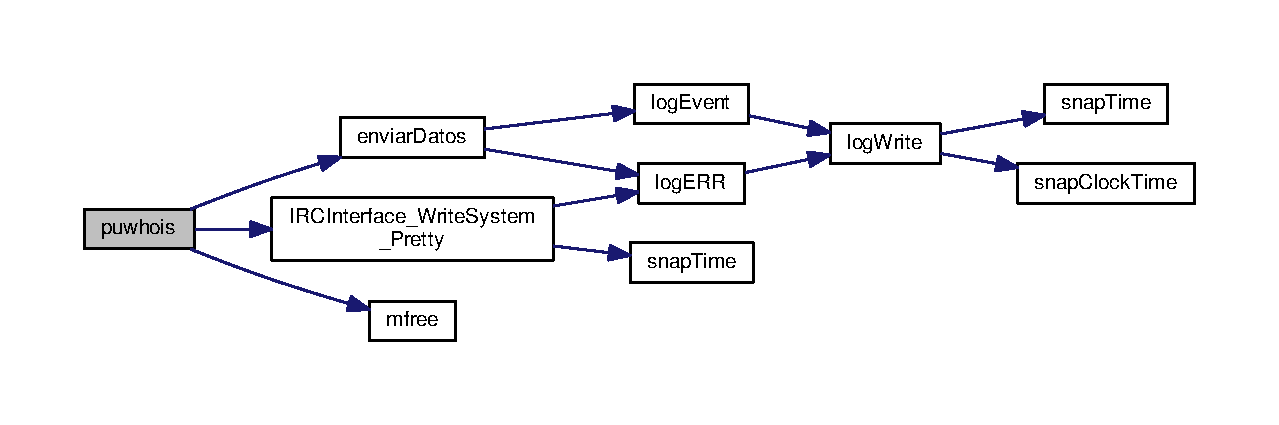
\includegraphics[width=350pt]{user__commands_8h_a08bd5900f288bfb5712d3f5ca6e624b6_cgraph}
\end{center}
\end{figure}




\subsection{Variable Documentation}
\hypertarget{user__commands_8h_a7e2f32e47f3780a66e19651d8e79bced}{\index{user\-\_\-commands.\-h@{user\-\_\-commands.\-h}!nick\-\_\-user@{nick\-\_\-user}}
\index{nick\-\_\-user@{nick\-\_\-user}!user_commands.h@{user\-\_\-commands.\-h}}
\subsubsection[{nick\-\_\-user}]{\setlength{\rightskip}{0pt plus 5cm}char nick\-\_\-user\mbox{[}{\bf M\-A\-X\-D\-A\-T\-A}\mbox{]}}}\label{user__commands_8h_a7e2f32e47f3780a66e19651d8e79bced}
nick del usuario operador del cliente \hypertarget{user__commands_8h_ab5efd1efa144e252f4c5312ae57bea2e}{\index{user\-\_\-commands.\-h@{user\-\_\-commands.\-h}!recv\-\_\-tid@{recv\-\_\-tid}}
\index{recv\-\_\-tid@{recv\-\_\-tid}!user_commands.h@{user\-\_\-commands.\-h}}
\subsubsection[{recv\-\_\-tid}]{\setlength{\rightskip}{0pt plus 5cm}pthread\-\_\-t recv\-\_\-tid}}\label{user__commands_8h_ab5efd1efa144e252f4c5312ae57bea2e}
tid del hilo encargado de recibir datos del servidor

Globales útiles sobre la conexión del cliente con el servidor \hypertarget{user__commands_8h_acd63fb8dbd9439219e2db08dfc173aa0}{\index{user\-\_\-commands.\-h@{user\-\_\-commands.\-h}!sockfd\-\_\-user@{sockfd\-\_\-user}}
\index{sockfd\-\_\-user@{sockfd\-\_\-user}!user_commands.h@{user\-\_\-commands.\-h}}
\subsubsection[{sockfd\-\_\-user}]{\setlength{\rightskip}{0pt plus 5cm}int sockfd\-\_\-user}}\label{user__commands_8h_acd63fb8dbd9439219e2db08dfc173aa0}
global con el descriptor socket abierto con el servidor

descriptor con el socket abierto con el servidor 
\hypertarget{xchat2_8h}{}\section{includes/xchat2.h File Reference}
\label{xchat2_8h}\index{includes/xchat2.\+h@{includes/xchat2.\+h}}


Declaraciones de funciones, definición de tipos\+: implementación de los callbacks de xchat2.  


{\ttfamily \#include $<$redes2/ircxchat.\+h$>$}\\*
{\ttfamily \#include $<$redes2/irc.\+h$>$}\\*
{\ttfamily \#include $<$netdb.\+h$>$}\\*
{\ttfamily \#include $<$sys/types.\+h$>$}\\*
{\ttfamily \#include $<$sys/socket.\+h$>$}\\*
{\ttfamily \#include $<$netinet/in.\+h$>$}\\*
{\ttfamily \#include $<$arpa/inet.\+h$>$}\\*
{\ttfamily \#include $<$sys/ioctl.\+h$>$}\\*
{\ttfamily \#include $<$net/if.\+h$>$}\\*
{\ttfamily \#include \char`\"{}types.\+h\char`\"{}}\\*
{\ttfamily \#include \char`\"{}conexion\+\_\+tcp.\+h\char`\"{}}\\*
{\ttfamily \#include \char`\"{}logger.\+h\char`\"{}}\\*
{\ttfamily \#include \char`\"{}user\+\_\+commands.\+h\char`\"{}}\\*
{\ttfamily \#include \char`\"{}aux\+\_\+functions.\+h\char`\"{}}\\*
Include dependency graph for xchat2.\+h\+:
% FIG 0
This graph shows which files directly or indirectly include this file\+:
% FIG 1
\subsection*{Functions}
\begin{DoxyCompactItemize}
\item 
int \hyperlink{xchat2_8h_a41f93f364aea303a0c93177289733f92}{command\+\_\+query} (char $\ast$message)
\begin{DoxyCompactList}\small\item\em Parsea los mensajes y respuestas que recibe del servidor. \end{DoxyCompactList}\item 
void \hyperlink{xchat2_8h_a63f7dc08db4a2318cb526eee804709b3}{unpipe} (char $\ast$message, int M\+A\+X\+D\+A\+T\+A\+\_\+flag)
\begin{DoxyCompactList}\small\item\em Funcion para dividir en comandos la cadena \char`\"{}message\char`\"{}. \end{DoxyCompactList}\item 
void \hyperlink{xchat2_8h_a7230d43b8458797c679e7180bf1fda90}{receive\+\_\+messages} (void $\ast$no\+\_\+arg)
\begin{DoxyCompactList}\small\item\em Funcion ejecutada por un hilo, que recibe mensajes del servidor y los procesa segun el tipo de respuesta. \end{DoxyCompactList}\item 
void \hyperlink{xchat2_8h_a98484e1bbb136d37503aa6c604eff6a2}{glue\+And\+Query} (char $\ast$command, char $\ast$\hyperlink{xchat2_8c_a4e304440b657a8d3265793203cb12393}{last\+\_\+command})
\end{DoxyCompactItemize}
\subsection*{Variables}
\begin{DoxyCompactItemize}
\item 
\hyperlink{user__commands_8h_af6812f6f50dd2285ed021d5f1bd04b7a}{p\+\_\+funcion} \hyperlink{xchat2_8h_afe699fe3416e9bf2d3553e35d7a1dea2}{p\+\_\+array\+\_\+funciones} \mbox{[}57\mbox{]}
\end{DoxyCompactItemize}


\subsection{Detailed Description}
Declaraciones de funciones, definición de tipos\+: implementación de los callbacks de xchat2. 

\begin{DoxyAuthor}{Author}
Alfonso Sebares 

Beatriz de Pablo 

Celia Mateos 
\end{DoxyAuthor}
\begin{DoxyDate}{Date}
20/03/17 
\end{DoxyDate}


\subsection{Function Documentation}
\index{xchat2.\+h@{xchat2.\+h}!command\+\_\+query@{command\+\_\+query}}
\index{command\+\_\+query@{command\+\_\+query}!xchat2.\+h@{xchat2.\+h}}
\subsubsection[{\texorpdfstring{command\+\_\+query(char $\ast$message)}{command_query(char *message)}}]{\setlength{\rightskip}{0pt plus 5cm}int command\+\_\+query (
\begin{DoxyParamCaption}
\item[{char $\ast$}]{message}
\end{DoxyParamCaption}
)}\hypertarget{xchat2_8h_a41f93f364aea303a0c93177289733f92}{}\label{xchat2_8h_a41f93f364aea303a0c93177289733f92}


Parsea los mensajes y respuestas que recibe del servidor. 


\begin{DoxyParams}{Parameters}
{\em massage} & mensaje recibido para procesar \\
\hline
\end{DoxyParams}
\begin{DoxyReturn}{Returns}
OK si todo fue correcto y E\+RR si ocurrio un error 
\end{DoxyReturn}
$<$ delimitador para separar mensajes 
\begin{DoxyCode}
40                                 \{
41 
42         \textcolor{keywordtype}{long} ret = -1;
43         \textcolor{keywordtype}{int} retorno = -1;
44         \textcolor{keywordtype}{char} *\hyperlink{_g-2361-06-_p1-_server_8c_ad2849cf781a4db22cc1b31eaaee50a4f}{prefix} = NULL;
45         \textcolor{keywordtype}{int} n = -1;
46         \textcolor{keywordtype}{int} counter = 1;
47     \textcolor{keywordtype}{char} mensaje[\hyperlink{types_8h_ae7e715c270481406658bbd2bafa2897f}{MAXDATA}] = \{0\};
48     \textcolor{keywordtype}{char} mensajeLargo[10*\hyperlink{types_8h_ae7e715c270481406658bbd2bafa2897f}{MAXDATA}] = \{0\};
49     \textcolor{keywordtype}{char} *\hyperlink{_g-2361-06-_p1-_server_8c_a32d2f5216cddb59c7cc8fb2806a7e727}{msg} = NULL;
50     \textcolor{keywordtype}{char} *\hyperlink{_g-2361-06-_p1-_server_8c_a89f27568c92a418413e6b37b41f07e21}{nick} = NULL;
51     \textcolor{keywordtype}{char} *nick2 = NULL;
52     \textcolor{comment}{//002}
53     \textcolor{keywordtype}{char} *servername = NULL;
54         \textcolor{keywordtype}{char} *versionname = NULL;
55         \textcolor{comment}{//003}
56         \textcolor{keywordtype}{char} *timedate = NULL;
57         \textcolor{comment}{//004}
58         \textcolor{keywordtype}{char}* version = NULL;
59         \textcolor{keywordtype}{char}* availableusermodes = NULL;
60         \textcolor{keywordtype}{char}* availablechannelmodes = NULL;
61         \textcolor{keywordtype}{char}* addedg = NULL;    
62         \textcolor{comment}{//251}
63         \textcolor{keywordtype}{int} nusers = 0;
64         \textcolor{keywordtype}{int} ninvisibles = 0;
65         \textcolor{keywordtype}{int} nservers = 0;
66         \textcolor{keywordtype}{char} *type = NULL;
67         \textcolor{comment}{//char **parameters = NULL;}
68         \textcolor{comment}{//int numparameters = 0;}
69 
70         \textcolor{comment}{//265}
71         \textcolor{keywordtype}{char} *substring = NULL;
72         \textcolor{comment}{//322}
73         \textcolor{keywordtype}{char} *visible = NULL;
74         \textcolor{comment}{//332}
75         \textcolor{keywordtype}{char} *\hyperlink{_g-2361-06-_p1-_server_8c_affecb48e716753e10b44feac31f12529}{topic} = NULL;
76         \textcolor{keywordtype}{char} *\hyperlink{_g-2361-06-_p1-_server_8c_a842ca2f026578e5c479c095ff3335969}{channel} = NULL;
77 
78         \textcolor{comment}{//353}
79         \textcolor{comment}{//char* show\_nick;}
80 
81         \textcolor{comment}{//JOIN}
82         \textcolor{keywordtype}{char}* \hyperlink{_g-2361-06-_p1-_server_8c_a5892a9181e6a332f84d27aecd41dcd12}{key} = NULL;    
83         \textcolor{keywordtype}{char} command[\hyperlink{types_8h_ae7e715c270481406658bbd2bafa2897f}{MAXDATA}];
84 
85         \textcolor{comment}{//PRIVMSG}
86         \textcolor{keywordtype}{char}* \hyperlink{_g-2361-06-_p1-_server_8c_a968dcc7e43caeca7959f3c069dcccc6a}{msgtarget} = NULL;
87         \textcolor{keywordtype}{char}* origin\_nick = NULL;
88         \textcolor{keywordtype}{char} nick\_privmsg[\hyperlink{types_8h_ae7e715c270481406658bbd2bafa2897f}{MAXDATA}];
89         \textcolor{keywordtype}{char} *filename = NULL, *hostname\_destino = NULL;
90         \textcolor{keywordtype}{unsigned} \textcolor{keywordtype}{long} length, port;
91 
92         \textcolor{comment}{//PART}
93         \textcolor{keywordtype}{char}* nick\_part;
94         \textcolor{keywordtype}{char}* username\_part;
95         \textcolor{keywordtype}{char}* host\_part;
96         \textcolor{keywordtype}{char}* server\_part;
97 
98         \textcolor{comment}{//PING}
99         \textcolor{keywordtype}{char}* server, *\hyperlink{_g-2361-06-_p1-_server_8c_a70dd311bef3d0b4160a7ce0706f8f4cc}{server2};
100         \textcolor{keywordtype}{char}* command\_pong;
101 
102         \textcolor{comment}{//Strtok}
103         \textcolor{keyword}{const} \textcolor{keywordtype}{char} s[2] = \textcolor{stringliteral}{":"}; 
104         \textcolor{keywordtype}{char} *token = NULL;
105 
106         \textcolor{comment}{//472}
107         \textcolor{keywordtype}{char} *modechar = NULL;
108 
109         \textcolor{comment}{//MODE}
110         \textcolor{keywordtype}{char} *\hyperlink{_g-2361-06-_p1-_server_8c_a55a7bd8f3229706c5917445aba995c5b}{channeluser} = NULL;
111         \textcolor{keywordtype}{char} *mode = NULL;
112         \textcolor{keywordtype}{char} *\hyperlink{_g-2361-06-_p1-_server_8c_a14871705f45ccdc5bb9f4549efd8e119}{user} = NULL;
113 
114         \textcolor{comment}{//KICK}
115         \textcolor{keywordtype}{char} *comment = NULL;
116 
117         \textcolor{comment}{//QUIT}
118         \textcolor{keywordtype}{char} **channelsQuit;
119         \textcolor{keywordtype}{int} numChannelsQuit;
120         \textcolor{keywordtype}{int} i;
121         \textcolor{comment}{//char* realname, *host;}
122 
123         \textcolor{comment}{//GENERAL}
124         \textcolor{keywordtype}{char} **params;
125         \textcolor{keywordtype}{int} n\_params;
126         \textcolor{keywordtype}{int} unknw\_type;
127         \textcolor{keyword}{const} \textcolor{keywordtype}{char} space\_delim[2] = \textcolor{stringliteral}{" "};
128         \textcolor{keywordtype}{char} *message\_cp = NULL;
129 
130         \textcolor{comment}{//g\_print("Mesaje recibido en command\_query: %s", message);}
131 
132         \textcolor{comment}{/*}
133 \textcolor{comment}{        if(message == NULL) \{}
134 \textcolor{comment}{                g\_print(RED "ERROR - In command\_query: message == NULL al principio\(\backslash\)n\(\backslash\)n" RESET);}
135 \textcolor{comment}{                return ERR;}
136 \textcolor{comment}{        \}}
137 \textcolor{comment}{        */}
138 
139         IRCInterface\_PlaneRegisterInMessage(message);
140 
141         \textcolor{keywordflow}{switch}(IRC\_CommandQuery(message))\{
142                 \textcolor{keywordflow}{case} RPL\_WELCOME: \textcolor{comment}{//001}
143                         ret = IRCParse\_RplWelcome(message, &prefix, &nick2, &msg);
144                         \textcolor{keywordflow}{if}(ret != IRC\_OK)\{
145                                 g\_print(\hyperlink{types_8h_a8d23feea868a983c8c2b661e1e16972f}{RED} \textcolor{stringliteral}{"\(\backslash\)nERROR - In command\_query: case RPL\_WELCOME -
       IRCParse\_RplWelcome != IRC\_OK"} \hyperlink{types_8h_ab702106cf3b3e96750b6845ded4e0299}{RESET});
146                                 \textcolor{comment}{//return IRCERR\_NOCONNECT;}
147                         \}
148                         g\_print(\textcolor{stringliteral}{"Comandos recibidos en el IRCParse\_RplWelcome: \(\backslash\)n"});
149                         g\_print(\textcolor{stringliteral}{"\(\backslash\)t message: %s \(\backslash\)n"},message);
150                         g\_print(\textcolor{stringliteral}{"\(\backslash\)t prefix: %s \(\backslash\)n"},prefix);
151                         g\_print(\textcolor{stringliteral}{"\(\backslash\)t nick2: %s \(\backslash\)n"},nick2);
152                         g\_print(\textcolor{stringliteral}{"\(\backslash\)t msg: %s \(\backslash\)n\(\backslash\)n"},msg);
153                         \textcolor{comment}{//obtenemos el hostname, util para el envio de ficheros}
154                         \hyperlink{xchat2_8c_af203df082d5c6dcaa0c88b07cf86466d}{hostname} = strtok(msg, \textcolor{stringliteral}{" "});
155                         \textcolor{keywordflow}{while} (((\hyperlink{xchat2_8c_af203df082d5c6dcaa0c88b07cf86466d}{hostname} = strtok(NULL, \textcolor{stringliteral}{" "})) != NULL) && (counter < 5))\{
156                                 counter++;
157                         \}
158                         \hyperlink{xchat2_8c_af203df082d5c6dcaa0c88b07cf86466d}{hostname} = strtok(NULL, \textcolor{stringliteral}{" "});
159                         g\_print(\textcolor{stringliteral}{"\(\backslash\)t hostname: %s \(\backslash\)n\(\backslash\)n"}, \hyperlink{xchat2_8c_af203df082d5c6dcaa0c88b07cf86466d}{hostname});
160                         \hyperlink{aux__functions_8h_a043ae6695458ae3a85dc9da43cf9b751}{IRCInterface\_WriteSystemThread\_Pretty}(\textcolor{stringliteral}{"*"}, msg
      );
161                         \textcolor{keywordflow}{break};
162 
163                 \textcolor{keywordflow}{case} RPL\_YOURHOST:      \textcolor{comment}{//002}
164                         \textcolor{comment}{//long IRCParse\_RplYourHost (char *strin, char **prefix, char **nick, char **msg,
       char **servername, char **versionname)}
165                         ret = IRCParse\_RplYourHost(message, &prefix, &nick2, &msg, &servername, &
      versionname);
166                         \textcolor{keywordflow}{if}(ret != IRC\_OK)\{
167                                 g\_print(\hyperlink{types_8h_a8d23feea868a983c8c2b661e1e16972f}{RED} \textcolor{stringliteral}{"\(\backslash\)nERROR - In command\_query: case RPL\_YOURHOST -
       IRCParse\_RplYourHost != IRC\_OK"} \hyperlink{types_8h_ab702106cf3b3e96750b6845ded4e0299}{RESET});
168                                 \textcolor{comment}{//return IRCERR\_NOCONNECT;}
169                         \}
170                         g\_print(\textcolor{stringliteral}{"Comandos recibidos en el IRCParse\_RplYourHost: \(\backslash\)n"});
171                         g\_print(\textcolor{stringliteral}{"\(\backslash\)t message: %s \(\backslash\)n"},message);
172                         g\_print(\textcolor{stringliteral}{"\(\backslash\)t prefix: %s \(\backslash\)n"},prefix);
173                         g\_print(\textcolor{stringliteral}{"\(\backslash\)t nick2: %s \(\backslash\)n"},nick2);
174                         g\_print(\textcolor{stringliteral}{"\(\backslash\)t servername: %s \(\backslash\)n"},servername);
175                         g\_print(\textcolor{stringliteral}{"\(\backslash\)t versionname: %s \(\backslash\)n"},versionname);           
176                         g\_print(\textcolor{stringliteral}{"\(\backslash\)t msg: %s \(\backslash\)n\(\backslash\)n"},msg);
177                         \hyperlink{aux__functions_8h_a043ae6695458ae3a85dc9da43cf9b751}{IRCInterface\_WriteSystemThread\_Pretty}(\textcolor{stringliteral}{"*"},msg)
      ;
178                         \textcolor{keywordflow}{break};
179 
180                 \textcolor{keywordflow}{case} RPL\_CREATED:\textcolor{comment}{//003                  }
181                         \textcolor{comment}{//long IRCParse\_RplCreated (char *strin, char **prefix, char **nick,char
       **timedate, char **msg)}
182                         ret = IRCParse\_RplCreated(message, &prefix, &nick2, &timedate, &msg);
183                         \textcolor{keywordflow}{if}(ret != IRC\_OK)\{
184                                 g\_print(\hyperlink{types_8h_a8d23feea868a983c8c2b661e1e16972f}{RED} \textcolor{stringliteral}{"\(\backslash\)nERROR - In command\_query: case RPL\_CREATED -
       IRCParse\_RplCreated != IRC\_OK"} \hyperlink{types_8h_ab702106cf3b3e96750b6845ded4e0299}{RESET});
185                                 \textcolor{comment}{//return IRCERR\_NOCONNECT;}
186                         \}
187                         g\_print(\textcolor{stringliteral}{"Comandos recibidos en el IRCParse\_RplCreated: \(\backslash\)n"});
188                         g\_print(\textcolor{stringliteral}{"\(\backslash\)t message: %s \(\backslash\)n"},message);
189                         g\_print(\textcolor{stringliteral}{"\(\backslash\)t prefix: %s \(\backslash\)n"},prefix);
190                         g\_print(\textcolor{stringliteral}{"\(\backslash\)t nick2: %s \(\backslash\)n"},nick2);
191                         g\_print(\textcolor{stringliteral}{"\(\backslash\)t timedate: %s \(\backslash\)n"},timedate); 
192                         g\_print(\textcolor{stringliteral}{"\(\backslash\)t msg: %s \(\backslash\)n\(\backslash\)n"},msg);
193                         \hyperlink{aux__functions_8h_a043ae6695458ae3a85dc9da43cf9b751}{IRCInterface\_WriteSystemThread\_Pretty}(\textcolor{stringliteral}{"*"},msg)
      ;
194                         \textcolor{keywordflow}{break};
195 
196                 \textcolor{keywordflow}{case} RPL\_MYINFO: \textcolor{comment}{//004}
197                         \textcolor{comment}{//long IRCParse\_RplMyInfo (char *strin, char **prefix, char **nick, char
       **servername, char **version, char **availableusermodes, char **availablechannelmodes, char **addedg)}
198                         ret = IRCParse\_RplMyInfo(message, &prefix, &nick2, &servername, &version, &
      availableusermodes, &availablechannelmodes, &addedg);
199                         \textcolor{keywordflow}{if}(ret != IRC\_OK)\{
200                                 g\_print(\hyperlink{types_8h_a8d23feea868a983c8c2b661e1e16972f}{RED} \textcolor{stringliteral}{"\(\backslash\)nERROR - In command\_query: case RPL\_MYINFO -
       IRCParse\_RplMyInfo != IRC\_OK"} \hyperlink{types_8h_ab702106cf3b3e96750b6845ded4e0299}{RESET});
201                                 \textcolor{comment}{//return IRCERR\_NOCONNECT;}
202                         \}
203                         g\_print(\textcolor{stringliteral}{"Comandos recibidos en el IRCParse\_RplMyInfo: \(\backslash\)n"});
204                         g\_print(\textcolor{stringliteral}{"\(\backslash\)t message: %s \(\backslash\)n"},message);
205                         g\_print(\textcolor{stringliteral}{"\(\backslash\)t prefix: %s \(\backslash\)n"},prefix);
206                         g\_print(\textcolor{stringliteral}{"\(\backslash\)t nick2: %s \(\backslash\)n"},nick2);
207                         g\_print(\textcolor{stringliteral}{"\(\backslash\)t servername: %s \(\backslash\)n"},servername);
208                         g\_print(\textcolor{stringliteral}{"\(\backslash\)t version: %s \(\backslash\)n"},version);
209                         g\_print(\textcolor{stringliteral}{"\(\backslash\)t availableusermodes: %s \(\backslash\)n"},availableusermodes);     
210                         g\_print(\textcolor{stringliteral}{"\(\backslash\)t availablechannelmodes: %s \(\backslash\)n"},availablechannelmodes);
211                         g\_print(\textcolor{stringliteral}{"\(\backslash\)t addedg: %s \(\backslash\)n\(\backslash\)n"},addedg);
212                         n = snprintf(mensaje, \textcolor{keyword}{sizeof} mensaje,\textcolor{stringliteral}{"%s %s %s %s %s "},servername,version,
      availableusermodes,availablechannelmodes,addedg);
213 
214                         \textcolor{keywordflow}{if} ( n < 0 || n >= \textcolor{keyword}{sizeof} mensaje )\{
215                                 g\_print(\textcolor{stringliteral}{"Error en sprintf \(\backslash\)n"});
216                         \textcolor{keywordflow}{return} \hyperlink{types_8h_a735563036dced0b7d6cc98f97ea4978b}{ERR};    \textcolor{comment}{// or other error handling}
217                         \}
218                         \hyperlink{aux__functions_8h_a043ae6695458ae3a85dc9da43cf9b751}{IRCInterface\_WriteSystemThread\_Pretty}(\textcolor{stringliteral}{"*"},
      mensaje);            
219                         \textcolor{keywordflow}{break};
220 
221                 \textcolor{keywordflow}{case} RPL\_BOUNCE: \textcolor{comment}{//005}
222                         \textcolor{comment}{//   long IRCParse\_RplISupport (char *strin, char **prefix, char **nick, char
       **msg)                                                }
223                         ret = IRCParse\_RplISupport(message, &prefix, &nick2, &msg);
224                         \textcolor{keywordflow}{if}(ret != IRC\_OK)\{
225                                 g\_print(\hyperlink{types_8h_a8d23feea868a983c8c2b661e1e16972f}{RED} \textcolor{stringliteral}{"\(\backslash\)nERROR - In command\_query: case RPL\_BOUNCE
       -IRCParse\_RplISupport != IRC\_OK"} \hyperlink{types_8h_ab702106cf3b3e96750b6845ded4e0299}{RESET});
226                                 \textcolor{comment}{//return IRCERR\_NOCONNECT;}
227                         \}
228                         g\_print(\textcolor{stringliteral}{"Comandos recibidos en el IRCParse\_RplISupport: \(\backslash\)n"});
229                         g\_print(\textcolor{stringliteral}{"\(\backslash\)t message: %s \(\backslash\)n"},message);
230                         g\_print(\textcolor{stringliteral}{"\(\backslash\)t prefix: %s \(\backslash\)n"},prefix);
231                         g\_print(\textcolor{stringliteral}{"\(\backslash\)t nick2: %s \(\backslash\)n"},nick2);
232                         g\_print(\textcolor{stringliteral}{"\(\backslash\)t msg: %s \(\backslash\)n\(\backslash\)n"},msg);
233                         \hyperlink{aux__functions_8h_a043ae6695458ae3a85dc9da43cf9b751}{IRCInterface\_WriteSystemThread\_Pretty}(\textcolor{stringliteral}{"*"},msg)
      ;                
234                         \textcolor{keywordflow}{break};
235 
236                 \textcolor{keywordflow}{case} RPL\_LUSERCLIENT: \textcolor{comment}{//251}
237                         \textcolor{comment}{//long IRCParse\_RplLuserClient (char *strin, char **prefix, char **nick, char
       **msg, int *nusers, int *ninvisibles, int *nservers)}
238                         
239                         ret = IRCParse\_RplLuserClient(message, &prefix, &nick2, &msg, &nusers, &ninvisibles
      , &nservers);
240                         \textcolor{keywordflow}{if}(ret != IRC\_OK)\{
241                                 g\_print(\hyperlink{types_8h_a8d23feea868a983c8c2b661e1e16972f}{RED} \textcolor{stringliteral}{"\(\backslash\)nERROR - In command\_query: case RPL\_LUSERCLIENT
       -IRCParse\_RplLuserClient != IRC\_OK"} \hyperlink{types_8h_ab702106cf3b3e96750b6845ded4e0299}{RESET});
242                                 \textcolor{comment}{//return IRCERR\_NOCONNECT;}
243                         \}
244                         g\_print(\textcolor{stringliteral}{"\(\backslash\)t message: %s \(\backslash\)n"},message);
245                         g\_print(\textcolor{stringliteral}{"\(\backslash\)t prefix: %s \(\backslash\)n"},prefix);
246                         g\_print(\textcolor{stringliteral}{"\(\backslash\)t nick2: %s \(\backslash\)n"},nick2);
247                         g\_print(\textcolor{stringliteral}{"\(\backslash\)t msg: %s \(\backslash\)n"},msg);
248                         g\_print(\textcolor{stringliteral}{"\(\backslash\)t nusers: %d \(\backslash\)n"},nusers);
249                         g\_print(\textcolor{stringliteral}{"\(\backslash\)t ninvisibles: %d \(\backslash\)n"},ninvisibles);
250                         g\_print(\textcolor{stringliteral}{"\(\backslash\)t nservers: %d \(\backslash\)n\(\backslash\)n"},nservers); 
251 
252                         \textcolor{comment}{/*ret\_strstr = strstr(mensaje,"nicknick");}
253 \textcolor{comment}{                        IRCInterface\_WriteSystem("*",ret\_strstr);*/} 
254 
255                         sprintf(mensaje,\textcolor{stringliteral}{"There are %d users and %d invisibles on %d servers "},nusers,
      ninvisibles,nservers);
256                         \textcolor{comment}{//sprintf(mensaje,"There are 13 users and 0 services on 1 servers");}
257 
258                         \hyperlink{aux__functions_8h_a043ae6695458ae3a85dc9da43cf9b751}{IRCInterface\_WriteSystemThread\_Pretty}(\textcolor{stringliteral}{"*"},
      mensaje);                                                                                                    
259                         \textcolor{keywordflow}{break};
260                         
261                 \textcolor{keywordflow}{case} RPL\_LUSERCHANNELS: \textcolor{comment}{//254}
262                         g\_print(\textcolor{stringliteral}{"\(\backslash\)t message: %s \(\backslash\)n"},message);
263                         \textcolor{comment}{/*Coger el primer token*/}
264                         token = strtok(message,s);
265                         \textcolor{comment}{/*Ir por el resto*/}
266                         \textcolor{keywordflow}{if}(token != NULL)\{
267                                 token = strtok(NULL,s); 
268                         \}
269                         \hyperlink{aux__functions_8h_a043ae6695458ae3a85dc9da43cf9b751}{IRCInterface\_WriteSystemThread\_Pretty}(\textcolor{stringliteral}{"*"},
      token);
270 
271                         token = NULL;
272                         \textcolor{comment}{//IRCInterface\_WriteSystem("*",message);        }
273                         \textcolor{keywordflow}{break};
274 
275                 \textcolor{keywordflow}{case} RPL\_LUSERME : \textcolor{comment}{//255}
276                         g\_print(\textcolor{stringliteral}{"\(\backslash\)t message: %s \(\backslash\)n"},message);
277                         \textcolor{comment}{/*Coger el primer token*/}
278                         token = strtok(message,s);
279                         \textcolor{comment}{/*Ir por el resto*/}
280                         \textcolor{keywordflow}{if}(token != NULL)\{
281                                 token = strtok(NULL,s); 
282                         \}
283                         \hyperlink{aux__functions_8h_a043ae6695458ae3a85dc9da43cf9b751}{IRCInterface\_WriteSystemThread\_Pretty}(\textcolor{stringliteral}{"*"},
      token);
284 
285                         token = NULL;
286                         \textcolor{comment}{//IRCInterface\_WriteSystem("*",message);        }
287                         \textcolor{keywordflow}{break};
288 
289                 \textcolor{keywordflow}{case} RPL\_LOCALUSERS: \textcolor{comment}{//265}
290                         substring = \hyperlink{aux__functions_8h_a20f32d171da437faef7716e4b6e667dd}{strnext}(message, \textcolor{charliteral}{':'});
291                         \textcolor{keywordflow}{if} (substring)\{
292                                 substring = \hyperlink{aux__functions_8h_a20f32d171da437faef7716e4b6e667dd}{strnext}(substring, \textcolor{charliteral}{':'});
293                         \}
294                         \hyperlink{aux__functions_8h_a043ae6695458ae3a85dc9da43cf9b751}{IRCInterface\_WriteSystemThread\_Pretty}(\textcolor{stringliteral}{"*"},
      substring);
295 
296                         substring = NULL;
297                         \textcolor{keywordflow}{break};
298 
299                 \textcolor{keywordflow}{case} RPL\_GLOBALUSERS: \textcolor{comment}{//266}
300                         g\_print(\hyperlink{types_8h_aea69ffbacdcdf16c21b8c9961df84448}{GRN} \textcolor{stringliteral}{"\(\backslash\)n>> [server command] RPL\_GLOBALUSERS - message = %s\(\backslash\)n"} 
      \hyperlink{types_8h_ab702106cf3b3e96750b6845ded4e0299}{RESET}, message);
301                         substring = \hyperlink{aux__functions_8h_a20f32d171da437faef7716e4b6e667dd}{strnext}(message, \textcolor{charliteral}{':'});
302                         \textcolor{keywordflow}{if} (substring)\{
303                                 substring = \hyperlink{aux__functions_8h_a20f32d171da437faef7716e4b6e667dd}{strnext}(substring, \textcolor{charliteral}{':'});
304                         \}
305                         \hyperlink{aux__functions_8h_a043ae6695458ae3a85dc9da43cf9b751}{IRCInterface\_WriteSystemThread\_Pretty}(\textcolor{stringliteral}{"*"},
      substring);
306 
307                         substring = NULL;               
308                         \textcolor{keywordflow}{break};
309 
310                 \textcolor{keywordflow}{case} RPL\_LISTSTART: \textcolor{comment}{//321}
311                         g\_print(\hyperlink{types_8h_aea69ffbacdcdf16c21b8c9961df84448}{GRN} \textcolor{stringliteral}{"\(\backslash\)n>> [server command] RPL\_LISTSTART - message = %s\(\backslash\)n"} 
      \hyperlink{types_8h_ab702106cf3b3e96750b6845ded4e0299}{RESET}, message);
312                         token = strtok(message,s);
313                         \textcolor{keywordflow}{if}(token != NULL)\{
314                                 token = strtok(NULL,s); 
315                         \}
316                         \hyperlink{aux__functions_8h_a043ae6695458ae3a85dc9da43cf9b751}{IRCInterface\_WriteSystemThread\_Pretty}(\textcolor{stringliteral}{"*"},
      token);
317 
318                         \textcolor{keywordflow}{break};
319 
320                 \textcolor{keywordflow}{case} RPL\_LIST: \textcolor{comment}{//322}
321                         \textcolor{comment}{//   long IRCParse\_RplList (char *strin, char **prefix, char **nick, char
       **channel, char **visible, char **topic)}
322                         g\_print(\hyperlink{types_8h_aea69ffbacdcdf16c21b8c9961df84448}{GRN} \textcolor{stringliteral}{"\(\backslash\)n>> [server command] RPL\_LIST - message = %s\(\backslash\)n"} 
      \hyperlink{types_8h_ab702106cf3b3e96750b6845ded4e0299}{RESET}, message);
323                         ret = IRCParse\_RplList(message, &prefix, &nick2, &channel, &visible, &topic);
324                         \textcolor{keywordflow}{if}(ret != IRC\_OK)\{
325                                 g\_print(\hyperlink{types_8h_a8d23feea868a983c8c2b661e1e16972f}{RED} \textcolor{stringliteral}{"\(\backslash\)nERROR - In command\_query: case RPL\_LIST -
       IRCParse\_RplList != IRC\_OK"} \hyperlink{types_8h_ab702106cf3b3e96750b6845ded4e0299}{RESET});
326                                 \textcolor{comment}{//return IRCERR\_NOCONNECT;}
327                         \}
328                         g\_print(\textcolor{stringliteral}{"Comandos recibidos en el IRCParse\_RplList: \(\backslash\)n"});
329                         g\_print(\textcolor{stringliteral}{"\(\backslash\)t message: %s \(\backslash\)n"},message);
330                         g\_print(\textcolor{stringliteral}{"\(\backslash\)t prefix: %s \(\backslash\)n"},prefix);
331                         g\_print(\textcolor{stringliteral}{"\(\backslash\)t nick2: %s \(\backslash\)n"},nick2);
332                         g\_print(\textcolor{stringliteral}{"\(\backslash\)t channel: %s \(\backslash\)n"},channel);
333                         g\_print(\textcolor{stringliteral}{"\(\backslash\)t visible: %s \(\backslash\)n"},visible);
334                         g\_print(\textcolor{stringliteral}{"\(\backslash\)t topic: %s \(\backslash\)n\(\backslash\)n"},topic);
335 
336                         sprintf(mensajeLargo,\textcolor{stringliteral}{"%s \(\backslash\)t %s \(\backslash\)t %s"},channel,visible,topic);
337                         g\_print(\textcolor{stringliteral}{"Mensaje creado: %s \(\backslash\)n\(\backslash\)n"},mensajeLargo);
338 
339                         \hyperlink{aux__functions_8h_a043ae6695458ae3a85dc9da43cf9b751}{IRCInterface\_WriteSystemThread\_Pretty}(\textcolor{stringliteral}{"*"},
      mensajeLargo);
340                         \hyperlink{aux__functions_8h_a2480cc4793bf25a16cc731dc9d033582}{mfree}(5,prefix,nick2,channel,visible,topic);       
341                         \textcolor{keywordflow}{break};
342 
343                 \textcolor{keywordflow}{case} RPL\_LISTEND: \textcolor{comment}{//323}
344                         g\_print(\hyperlink{types_8h_aea69ffbacdcdf16c21b8c9961df84448}{GRN} \textcolor{stringliteral}{"\(\backslash\)n>> [server command] RPL\_LISTEND - message = %s\(\backslash\)n"} 
      \hyperlink{types_8h_ab702106cf3b3e96750b6845ded4e0299}{RESET}, message);
345                         \textcolor{comment}{/*Coger el primer token*/}
346                         token = strtok(message,s);
347                         \textcolor{comment}{/*Ir por el resto*/}
348                         \textcolor{keywordflow}{if}(token != NULL)\{
349                                 token = strtok(NULL,s); 
350                         \}
351                         \hyperlink{aux__functions_8h_a043ae6695458ae3a85dc9da43cf9b751}{IRCInterface\_WriteSystemThread\_Pretty}(\textcolor{stringliteral}{"*"},
      token);
352 
353                         token = NULL;
354                         \textcolor{comment}{//IRCInterface\_WriteSystem("*",message);                        }
355                         \textcolor{keywordflow}{break};
356 
357                 \textcolor{keywordflow}{case} RPL\_WHOREPLY: \textcolor{comment}{//352}
358                         g\_print(\hyperlink{types_8h_aea69ffbacdcdf16c21b8c9961df84448}{GRN} \textcolor{stringliteral}{"\(\backslash\)n>> [server command] RPL\_WHOREPLY - message = %s\(\backslash\)n"} 
      \hyperlink{types_8h_ab702106cf3b3e96750b6845ded4e0299}{RESET}, message);
359                         \textcolor{keywordflow}{break};
360 
361                 \textcolor{keywordflow}{case} RPL\_MOTDSTART: \textcolor{comment}{//375}
362                         g\_print(\textcolor{stringliteral}{"\(\backslash\)t message: %s \(\backslash\)n"},message);
363                         \textcolor{comment}{/*Coger el primer token*/}
364                         token = strtok(message,s);
365                         \textcolor{comment}{/*Ir por el resto*/}
366                         \textcolor{keywordflow}{if}(token != NULL)\{
367                                 token = strtok(NULL,s); 
368                         \}
369                         \hyperlink{aux__functions_8h_a043ae6695458ae3a85dc9da43cf9b751}{IRCInterface\_WriteSystemThread\_Pretty}(\textcolor{stringliteral}{"*"},
      token);
370 
371                         token = NULL;
372                         \textcolor{comment}{//IRCInterface\_WriteSystem("*",message);                        }
373                         \textcolor{keywordflow}{break};
374 
375                 \textcolor{keywordflow}{case} RPL\_MOTD: \textcolor{comment}{//372}
376                         g\_print(\textcolor{stringliteral}{"\(\backslash\)t message: %s \(\backslash\)n"},message);
377                         \textcolor{comment}{/*Coger el primer token*/}
378                         token = strtok(message,s);
379                         \textcolor{comment}{/*Ir por el resto*/}
380                         \textcolor{keywordflow}{if}(token != NULL)\{
381                                 token = strtok(NULL,s); 
382                         \}
383                         \hyperlink{aux__functions_8h_a043ae6695458ae3a85dc9da43cf9b751}{IRCInterface\_WriteSystemThread\_Pretty}(\textcolor{stringliteral}{"*"},
      token);
384 
385                         token = NULL;
386                         \textcolor{comment}{//IRCInterface\_WriteSystem("*",message);                }
387                         \textcolor{keywordflow}{break};
388 
389                 \textcolor{keywordflow}{case} RPL\_ENDOFMOTD: \textcolor{comment}{//376}
390                         g\_print(\textcolor{stringliteral}{"\(\backslash\)t message: %s \(\backslash\)n"},message);
391                         \textcolor{comment}{/*Coger el primer token*/}
392                         token = strtok(message,s);
393                         \textcolor{comment}{/*Ir por el resto*/}
394                         \textcolor{keywordflow}{if}(token != NULL)\{
395                                 token = strtok(NULL,s); 
396                         \}
397                         \hyperlink{aux__functions_8h_a043ae6695458ae3a85dc9da43cf9b751}{IRCInterface\_WriteSystemThread\_Pretty}(\textcolor{stringliteral}{"*"},
      token);
398 
399                         token = NULL;
400                         \textcolor{comment}{//IRCInterface\_WriteSystem("*",message);        }
401                         \textcolor{keywordflow}{return} 19;\textcolor{comment}{//cambiar por un define}
402                         \textcolor{keywordflow}{break};
403 
404                 \textcolor{keywordflow}{case} RPL\_TOPIC: \textcolor{comment}{//332}
405                         g\_print(\hyperlink{types_8h_aea69ffbacdcdf16c21b8c9961df84448}{GRN} \textcolor{stringliteral}{"\(\backslash\)n>> [server command] RPL\_TOPIC - message = %s\(\backslash\)n"} 
      \hyperlink{types_8h_ab702106cf3b3e96750b6845ded4e0299}{RESET}, message);
406                         \textcolor{comment}{//g\_print("\(\backslash\)n=======CASE RPL\_TOPIC=======\(\backslash\)n");}
407                         \textcolor{comment}{//IRCParse\_RplTopic (char *strin, char **prefix, char **nick, char **nick2, char
       **channel, char **msg)}
408                         ret = IRCParse\_RplTopic(message, &prefix, &nick, &channel, &topic);
409                         \textcolor{keywordflow}{if}(ret != IRC\_OK)\{
410                                 g\_print(\hyperlink{types_8h_a8d23feea868a983c8c2b661e1e16972f}{RED} \textcolor{stringliteral}{"ERROR - In command\_query: case RPL\_TOPIC -
       IRCParse\_RplTopic devolvio != IRC\_OK\(\backslash\)n"} \hyperlink{types_8h_ab702106cf3b3e96750b6845ded4e0299}{RESET});
411                                 \textcolor{comment}{//return IRCERR\_NOCONNECT;}
412                         \}
413                         g\_print(\textcolor{stringliteral}{"\(\backslash\)t message: %s \(\backslash\)n"},message);
414                         g\_print(\textcolor{stringliteral}{"\(\backslash\)t prefix: %s \(\backslash\)n"},prefix);
415                         g\_print(\textcolor{stringliteral}{"\(\backslash\)t nick: %s \(\backslash\)n"},nick);
416                         g\_print(\textcolor{stringliteral}{"\(\backslash\)t channel: %s \(\backslash\)n"},channel);
417                         g\_print(\textcolor{stringliteral}{"\(\backslash\)t topic: %s \(\backslash\)n\(\backslash\)n"},topic);
418                         sprintf(mensaje,\textcolor{stringliteral}{"El topic para %s es %s "},channel,topic);
419                         g\_print(\textcolor{stringliteral}{"Mensaje: %s \(\backslash\)n"},mensaje);
420                         g\_print(\textcolor{stringliteral}{"Existe canal: %d \(\backslash\)n"}, IRCInterface\_QueryChannelExistThread(channel));
421 
422                         \hyperlink{aux__functions_8h_a6400bb2b7979a2393f0e84b6646a24fe}{IRCInterface\_WriteChannelThread\_Pretty}(
      channel,\textcolor{stringliteral}{"*"},mensaje);  
423                         \textcolor{keywordflow}{break};
424 
425                 \textcolor{keywordflow}{case} RPL\_AWAY: \textcolor{comment}{//306}
426                         g\_print(\hyperlink{types_8h_aea69ffbacdcdf16c21b8c9961df84448}{GRN} \textcolor{stringliteral}{"\(\backslash\)n>> [server command] RPL\_AWAY - message = %s\(\backslash\)n"} 
      \hyperlink{types_8h_ab702106cf3b3e96750b6845ded4e0299}{RESET}, message);
427                         \textcolor{comment}{//>> :irc.eps.net 306 gomupo :You have been marked as being away}
428                         IRCParse\_RplAway (message, &prefix, &nick, &nick2, &msg);
429                         \hyperlink{aux__functions_8h_a043ae6695458ae3a85dc9da43cf9b751}{IRCInterface\_WriteSystemThread\_Pretty}(\textcolor{stringliteral}{"*"},msg)
      ;
430                         \textcolor{keywordflow}{break};
431 
432                 \textcolor{keywordflow}{case} TOPIC: \textcolor{comment}{//332}
433                         g\_print(\hyperlink{types_8h_aea69ffbacdcdf16c21b8c9961df84448}{GRN} \textcolor{stringliteral}{"\(\backslash\)n>> [server command] TOPIC - message = %s\(\backslash\)n"} 
      \hyperlink{types_8h_ab702106cf3b3e96750b6845ded4e0299}{RESET}, message);
434                         \textcolor{comment}{//   long IRCParse\_Topic (char *strin, char **prefix, char **channel, char **topic)}
435                         ret = IRCParse\_Topic (message, &prefix, &channel, &topic);
436                         \textcolor{keywordflow}{if}(ret != IRC\_OK)\{
437                                 g\_print(\hyperlink{types_8h_a8d23feea868a983c8c2b661e1e16972f}{RED} \textcolor{stringliteral}{"ERROR - In command\_query: case TOPIC - IRCParse\_Topic
       devolvio != IRC\_OK\(\backslash\)n"} \hyperlink{types_8h_ab702106cf3b3e96750b6845ded4e0299}{RESET});
438                                 \textcolor{keywordflow}{return} \hyperlink{types_8h_a735563036dced0b7d6cc98f97ea4978b}{ERR};
439                         \}
440 
441                         g\_print(\textcolor{stringliteral}{"\(\backslash\)t message: %s \(\backslash\)n"},message);
442                         g\_print(\textcolor{stringliteral}{"\(\backslash\)t prefix: %s \(\backslash\)n"},prefix);
443                         g\_print(\textcolor{stringliteral}{"\(\backslash\)t channel: %s \(\backslash\)n"},channel);
444                         g\_print(\textcolor{stringliteral}{"\(\backslash\)t topic: %s \(\backslash\)n\(\backslash\)n"},topic);
445                         sprintf(mensaje,\textcolor{stringliteral}{"El topic para %s es %s \(\backslash\)n"},channel,topic);
446                         g\_print(\textcolor{stringliteral}{"Mensaje: %s \(\backslash\)n"},mensaje);
447                         g\_print(\textcolor{stringliteral}{"Existe canal: %d \(\backslash\)n"}, IRCInterface\_QueryChannelExistThread(channel));
448 
449                         \hyperlink{aux__functions_8h_a6400bb2b7979a2393f0e84b6646a24fe}{IRCInterface\_WriteChannelThread\_Pretty}(
      channel,\textcolor{stringliteral}{"*"},mensaje);
450                         \textcolor{keywordflow}{break};
451 
452                 \textcolor{keywordflow}{case} RPL\_NOTOPIC:
453                         \textcolor{keywordflow}{break};
454 
455                 \textcolor{keywordflow}{case} RPL\_TOPICWHOTIME: \textcolor{comment}{//333}
456                         \textcolor{keywordflow}{break};  
457 
458                 \textcolor{keywordflow}{case} RPL\_NAMREPLY: \textcolor{comment}{//353 - reply del servidor de de punames()}
459                         g\_print(\hyperlink{types_8h_aea69ffbacdcdf16c21b8c9961df84448}{GRN} \textcolor{stringliteral}{"\(\backslash\)n>> [server command] RPL\_NAMREPLY - message = %s\(\backslash\)n"} 
      \hyperlink{types_8h_ab702106cf3b3e96750b6845ded4e0299}{RESET}, message);
460                         \textcolor{comment}{//long IRCParse\_RplNamReply (char *strin, char **prefix, char **nick, char **type,
       char **channel, char **msg)}
461                         ret = IRCParse\_RplNamReply(message, &prefix, &nick, &type, &channel, &msg);
462                         \textcolor{keywordflow}{if}(ret != IRC\_OK)\{
463                                 g\_print(\hyperlink{types_8h_a8d23feea868a983c8c2b661e1e16972f}{RED} \textcolor{stringliteral}{"ERROR - In command\_query: case RPL\_NAMREPLY -
       IRCParse\_RplNamReply devolvio != IRC\_OK\(\backslash\)n"} \hyperlink{types_8h_ab702106cf3b3e96750b6845ded4e0299}{RESET});
464                                 \textcolor{comment}{//return IRCERR\_NOCONNECT;}
465                         \}
466                         g\_print(\textcolor{stringliteral}{"\(\backslash\)t message: %s \(\backslash\)n"},message);
467                         g\_print(\textcolor{stringliteral}{"\(\backslash\)t prefix: %s \(\backslash\)n"},prefix);
468                         g\_print(\textcolor{stringliteral}{"\(\backslash\)t nick: %s \(\backslash\)n"},nick);
469                         g\_print(\textcolor{stringliteral}{"\(\backslash\)t type: %s \(\backslash\)n"},type);                                                         
470                         g\_print(\textcolor{stringliteral}{"\(\backslash\)t channel: %s \(\backslash\)n"},channel);
471                         g\_print(\textcolor{stringliteral}{"\(\backslash\)t msg: %s \(\backslash\)n\(\backslash\)n"},msg);
472 
473                         \textcolor{comment}{//Ojo, que pasa si es names?? sin join}
474                         \textcolor{comment}{//Añadir los nicks a la ventana de lad erecha. Pillarlos del WHO que se envía }
475                         \textcolor{comment}{//despues del join.}
476                         \textcolor{comment}{//OJO es una prueba del funcionamineto de IRCInterface\_AddNickChannel,}
477                         \textcolor{comment}{//los nicks deberían de ser partidos mediante uso strtok o algo parecido}
478                         \textcolor{comment}{//IRCInterface\_AddNickChannel (channel, msg, msg, msg, msg, VOICE);}
479                         \textcolor{comment}{//sprintf(mensaje,"Usuarios en %s: %s",channel,msg);}
480                         \textcolor{comment}{//IRCInterface\_WriteChannelThread(channel,"*",mensaje);}
481                         \hyperlink{aux__functions_8h_a09c2fcb81e148a2f23080a1671869f96}{interface\_mostrar\_nicks}(channel,msg);    
482                         \textcolor{keywordflow}{break};
483 
484                 \textcolor{keywordflow}{case} RPL\_ENDOFNAMES: \textcolor{comment}{//366}
485                         g\_print(\textcolor{stringliteral}{"Mensaje recibido en RPL\_ENDOFNAMES: \(\backslash\)n"});
486                         \textcolor{comment}{//long IRCParse\_RplEndOfNames (char *strin, char **prefix, char **nick, char
       **channel, char **msg)}
487                         ret = IRCParse\_RplEndOfNames(message, &prefix, &nick2, &channel, &msg);
488                         \textcolor{keywordflow}{if}(ret != IRC\_OK)\{
489                                 g\_print(\hyperlink{types_8h_a8d23feea868a983c8c2b661e1e16972f}{RED} \textcolor{stringliteral}{"ERROR - In command\_query: case RPL\_ENDOFNAMES -
       IRCParse\_RplEndOfNames devolvio != IRC\_OK\(\backslash\)n"} \hyperlink{types_8h_ab702106cf3b3e96750b6845ded4e0299}{RESET});
490                                 \textcolor{comment}{//return IRCERR\_NOCONNECT;}
491                         \}
492                         g\_print(\textcolor{stringliteral}{"\(\backslash\)t message: %s \(\backslash\)n"},message);
493                         g\_print(\textcolor{stringliteral}{"\(\backslash\)t prefix: %s \(\backslash\)n"},prefix);
494                         g\_print(\textcolor{stringliteral}{"\(\backslash\)t nick: %s \(\backslash\)n"},nick);                                                 
495                         g\_print(\textcolor{stringliteral}{"\(\backslash\)t channel: %s \(\backslash\)n"},channel);
496                         g\_print(\textcolor{stringliteral}{"\(\backslash\)t msg: %s \(\backslash\)n\(\backslash\)n"},msg);
497 
498                         \textcolor{comment}{//IRCInterface\_WriteChannelThread(channel,"*",msg);}
499                         \textcolor{keywordflow}{break};
500 
501                 \textcolor{keywordflow}{case} JOIN:
502                         g\_print(\hyperlink{types_8h_aea69ffbacdcdf16c21b8c9961df84448}{GRN} \textcolor{stringliteral}{"\(\backslash\)n>> [server command] JOIN - message = %s\(\backslash\)n"} 
      \hyperlink{types_8h_ab702106cf3b3e96750b6845ded4e0299}{RESET}, message);
503                         g\_print(\hyperlink{types_8h_af54a5a977c0c499323d656315f008ee0}{MAG} \textcolor{stringliteral}{"\(\backslash\)nJOIN es %ld con IRC\_CommandQuery\(\backslash\)n"} 
      \hyperlink{types_8h_ab702106cf3b3e96750b6845ded4e0299}{RESET}, IRC\_CommandQuery(message));
504                         g\_print(\hyperlink{types_8h_af54a5a977c0c499323d656315f008ee0}{MAG} \textcolor{stringliteral}{"\(\backslash\)nJOIN es %ld con IRCUser\_CommandQuery\(\backslash\)n"} RESET, 
      IRCUser\_CommandQuery(message));
505 
506                         ret = IRCParse\_Join (message, &prefix, &channel, &key, &msg);
507                         \textcolor{keywordflow}{if}(ret != IRC\_OK)\{
508                                 g\_print(\hyperlink{types_8h_a8d23feea868a983c8c2b661e1e16972f}{RED} \textcolor{stringliteral}{"\(\backslash\)nERROR - In command\_query: JOIN - IRCParse\_Join devolvio
       error\(\backslash\)n"} RESET);
509                                 \textcolor{keywordflow}{return} \hyperlink{types_8h_a735563036dced0b7d6cc98f97ea4978b}{ERR};
510                         \}
511                         g\_print(\textcolor{stringliteral}{"Comandos recibidos en el IRCParse\_Join: \(\backslash\)n"});
512                         g\_print(\textcolor{stringliteral}{"\(\backslash\)t message: %s \(\backslash\)n"},message);
513                         g\_print(\textcolor{stringliteral}{"\(\backslash\)t prefix: %s \(\backslash\)n"},prefix);
514                         g\_print(\textcolor{stringliteral}{"\(\backslash\)t channel: %s \(\backslash\)n"},channel);
515                         g\_print(\textcolor{stringliteral}{"\(\backslash\)t key: %s \(\backslash\)n"},key);
516                         g\_print(\textcolor{stringliteral}{"\(\backslash\)t msg: %s \(\backslash\)n\(\backslash\)n"},msg);
517 
518                         IRCInterface\_AddNewChannelThread(msg, 0);
519                         IRCParse\_ComplexUser(prefix, &nick\_part, &username\_part, &host\_part, &server\_part);
520                         sprintf(mensaje, \textcolor{stringliteral}{"%s (%s) se ha unido al canal"}, nick\_part, prefix);
521                         \textcolor{keywordflow}{if}(!strcmp(\hyperlink{xchat2_8c_a7e2f32e47f3780a66e19651d8e79bced}{nick\_user}, nick\_part))\{
522                                 IRCInterface\_WriteChannelThread(msg,\textcolor{stringliteral}{"*"}, \textcolor{stringliteral}{"Bienvenido al canal"});
523                         \} \textcolor{keywordflow}{else} \{
524                                 IRCInterface\_WriteChannelThread(msg,\textcolor{stringliteral}{"*"}, mensaje);
525                         \}
526                         \textcolor{comment}{//Actualizar al lista de usuarios}
527                         sprintf(mensaje,\textcolor{stringliteral}{"/names %s"},msg);
528                         retorno = \hyperlink{user__commands_8h_abaae116595df34db33e65e3d9d225103}{punames}(mensaje);
529                         \textcolor{keywordflow}{if}(retorno == \hyperlink{types_8h_a735563036dced0b7d6cc98f97ea4978b}{ERR})\{
530                                 g\_print(\textcolor{stringliteral}{"ERROR - JOIN - punames"});
531                                 \textcolor{keywordflow}{return} \hyperlink{types_8h_a735563036dced0b7d6cc98f97ea4978b}{ERR};                          
532                         \}
533                         \textcolor{keywordflow}{break};
534 
535                 \textcolor{keywordflow}{case} NAMES:
536                         g\_print(\hyperlink{types_8h_aea69ffbacdcdf16c21b8c9961df84448}{GRN} \textcolor{stringliteral}{"\(\backslash\)n>> [server command] NAMES - message = %s\(\backslash\)n"} RESET, message);
537                         g\_print(\hyperlink{types_8h_aea69ffbacdcdf16c21b8c9961df84448}{GRN} \textcolor{stringliteral}{"\(\backslash\)nNo hay nada aquí, revisar (?)"} RESET);
538                         \textcolor{keywordflow}{break};
539 
540                 \textcolor{keywordflow}{case} PRIVMSG:
541                         g\_print(\hyperlink{types_8h_aea69ffbacdcdf16c21b8c9961df84448}{GRN} \textcolor{stringliteral}{"\(\backslash\)n>> [server command] PRIVMSG - message = %s\(\backslash\)n"} RESET, message);
542                         ret = IRCParse\_Privmsg(message, &prefix, &msgtarget, &msg);
543                         \textcolor{keywordflow}{if}(ret != IRC\_OK)\{
544                                 g\_print(\hyperlink{types_8h_a8d23feea868a983c8c2b661e1e16972f}{RED} \textcolor{stringliteral}{"\(\backslash\)nERROR - In command\_query: IRCParse\_Privmsg devolvio !=
       IRC\_OK"} RESET);
545                                 \textcolor{keywordflow}{return} \hyperlink{types_8h_a735563036dced0b7d6cc98f97ea4978b}{ERR};
546                         \}
547                         \textcolor{comment}{//>> :gomupo!~gonzalo@119.181.218.87.dynamic.jazztel.es PRIVMSG gon :hola}
548                         \textcolor{keywordflow}{if} ((origin\_nick = strtok(prefix, \textcolor{stringliteral}{"!"})) != NULL)\{
549                                 strcpy(nick\_privmsg, origin\_nick);
550                         \}
551                         g\_print(\textcolor{stringliteral}{"\(\backslash\)t nick\_privmsg: %s \(\backslash\)n"},nick\_privmsg);
552                         g\_print(\textcolor{stringliteral}{"\(\backslash\)t prefix: %s \(\backslash\)n"},prefix);
553                         g\_print(\textcolor{stringliteral}{"\(\backslash\)t msgtarget: %s \(\backslash\)n"},msgtarget);
554                         g\_print(\textcolor{stringliteral}{"\(\backslash\)t msg: %s \(\backslash\)n\(\backslash\)n"},msg);
555 
556                         \textcolor{keywordflow}{if}(msg[0] == 1 || (msg[0] == \textcolor{charliteral}{':'} || msg[1] == 1)) \{ \textcolor{comment}{//envio de ficheros}
557                                 g\_print(\textcolor{stringliteral}{"alguien quiere enviarme un fichero\(\backslash\)n"});
558                                 \textcolor{comment}{//char *msg = "\(\backslash\)001FSEND gato.jpg ~cgs@cliente168.wlan.uam.es 1234 24422";}
559                                 
560                                 filename = strtok(msg, \textcolor{stringliteral}{" "});
561                                 filename = strtok(NULL, \textcolor{stringliteral}{" "});
562                                 hostname\_destino = strtok(NULL, \textcolor{stringliteral}{" "});
563                                 port = (\textcolor{keywordtype}{unsigned} long) atol(strtok(NULL, \textcolor{stringliteral}{" "}));
564                                 length = (\textcolor{keywordtype}{unsigned} long) atol(strtok(NULL, \textcolor{stringliteral}{" "}));
565                                 g\_print(\textcolor{stringliteral}{"filename: %s \(\backslash\)n"},filename);
566                                 g\_print(\textcolor{stringliteral}{"hostname\_destino: %s \(\backslash\)n"},hostname\_destino);
567                                 g\_print(\textcolor{stringliteral}{"length: %ld \(\backslash\)n"},length);
568                                 g\_print(\textcolor{stringliteral}{"port: %ld \(\backslash\)n"},port);
569 
570                                 \textcolor{keywordflow}{if}(IRCInterface\_ReceiveDialogThread(\hyperlink{xchat2_8c_a7e2f32e47f3780a66e19651d8e79bced}{nick\_user}, filename) == TRUE)\{
571                                         g\_print(\textcolor{stringliteral}{"Lanzamos el hilo que guarda el archivo\(\backslash\)n"});
572                                         \textcolor{comment}{//pthread\_t tid;}
573 
574                                         \hyperlink{struct_file__args}{File\_args} args;
575                                         args.\hyperlink{struct_file__args_a9aa177aea3a099397a09131a92f30115}{hostname} = hostname\_destino;
576                                         args.\hyperlink{struct_file__args_ad24dfcb255f29ee677793a0051c7336b}{filename} = filename;
577                                         args.\hyperlink{struct_file__args_a83e78eb2ebacdc7e63eca61d1340fa61}{port} = port;
578                                         args.\hyperlink{struct_file__args_a3168e8734e7ad263d88a6da49b4aff20}{length} = length;
579 
580                                         \textcolor{keywordflow}{if}(pthread\_create( &\hyperlink{xchat2_8c_a808d33eb5e54db312802ea4b22189ef3}{sendf\_tid}, NULL, (\textcolor{keywordtype}{void}*) 
      \hyperlink{aux__functions_8h_a9a7f9a514711f5954007dc83533d9362}{save\_file}, (\textcolor{keywordtype}{void}*) &args) < 0)\{
581                                         g\_print(\textcolor{stringliteral}{"Error en la llamada a save\_file\(\backslash\)n"});
582                                                 \textcolor{keywordflow}{return} \hyperlink{types_8h_a735563036dced0b7d6cc98f97ea4978b}{ERR};
583                                         \}
584                                         \textcolor{keywordflow}{break};
585                                 \}
586                                 \textcolor{comment}{/*}
587 \textcolor{comment}{                                if (sscanf(msg, "\(\backslash\)001AUDIOCHAT %ms %li", &hostname\_destino, &port) > 0) \{}
588 \textcolor{comment}{                                        g\_print("host=%s, port=%li\(\backslash\)n", hostname\_destino, port);}
589 \textcolor{comment}{                                \} else\{}
590 \textcolor{comment}{                                        g\_print("Formato incorrecto en envio de fichero\(\backslash\)n");}
591 \textcolor{comment}{                                \}*/}
592                                 ret = \hyperlink{conexion__tcp_8h_ab9468ce1338cfca5736ab407ba155f55}{enviarDatos}(\hyperlink{xchat2_8c_acd63fb8dbd9439219e2db08dfc173aa0}{sockfd\_user}, command, strlen(
      command));
593                                 \textcolor{keywordflow}{if}(ret < 0)\{
594                                         g\_print(\hyperlink{types_8h_a8d23feea868a983c8c2b661e1e16972f}{RED} \textcolor{stringliteral}{"ERROR - In command\_query: case PRIVMSG -
       enviarDatos() devolvio error (ver secuencia en .log)\(\backslash\)n\(\backslash\)t\(\backslash\)tEl cliente se cerrará.\(\backslash\)n"} RESET);
595                                         exit(1);
596                                 \}
597                                 \textcolor{keywordflow}{if}(ret == 0)\{ \textcolor{comment}{//timeout }
598                                         g\_print(\hyperlink{types_8h_a8d23feea868a983c8c2b661e1e16972f}{RED} \textcolor{stringliteral}{"ERROR - In command\_query: case PRIVMSG -
       enviarDatos() mandó 0 Bytes(ver secuencia en .log)\(\backslash\)n\(\backslash\)t\(\backslash\)t(Timeout de conexión probablemente)\(\backslash\)n"} RESET);
599                                         exit(1);
600                                 \}
601                         \}
602 
603                         \textcolor{keywordflow}{if}(msgtarget[0] != \textcolor{charliteral}{'#'})\{\textcolor{comment}{//no grupo}
604                                 IRCInterface\_AddNewChannelThread(nick\_privmsg, 0);                              
605                                 \hyperlink{aux__functions_8h_a6400bb2b7979a2393f0e84b6646a24fe}{IRCInterface\_WriteChannelThread\_Pretty}
      (nick\_privmsg, nick\_privmsg, msg);
606                                 \textcolor{keywordflow}{return} \hyperlink{daemon_8h_aba51915c87d64af47fb1cc59348961c9}{OK};
607                         \}
608 
609                         \textcolor{comment}{//IRCInterface\_WriteChannelThread(msgtarget, nick\_privmsg, msg);}
610                         \hyperlink{aux__functions_8h_a6400bb2b7979a2393f0e84b6646a24fe}{IRCInterface\_WriteChannelThread\_Pretty}(
      msgtarget, nick\_privmsg, msg);
611                         \textcolor{keywordflow}{break};
612 
613                 \textcolor{keywordflow}{case} PART:
614                         g\_print(\hyperlink{types_8h_aea69ffbacdcdf16c21b8c9961df84448}{GRN} \textcolor{stringliteral}{"\(\backslash\)n>> [server command] PART - message = %s\(\backslash\)n"} RESET, message);
615                         ret = IRCParse\_Part (message, &prefix, &channel, &msg);
616                         \textcolor{keywordflow}{if}(ret != IRC\_OK)\{
617                                 g\_print(\hyperlink{types_8h_a8d23feea868a983c8c2b661e1e16972f}{RED} \textcolor{stringliteral}{"\(\backslash\)nERROR - In command\_query: case PART - IRCParse\_Part
       devolvio != IRC\_OK"} RESET);
618                                 \textcolor{keywordflow}{return} \hyperlink{types_8h_a735563036dced0b7d6cc98f97ea4978b}{ERR};
619                         \}
620                         g\_print(\textcolor{stringliteral}{"Comandos recibidos en el IRCParse\_PART: \(\backslash\)n"});
621                         g\_print(\textcolor{stringliteral}{"\(\backslash\)t message: %s \(\backslash\)n"},message);
622                         g\_print(\textcolor{stringliteral}{"\(\backslash\)t prefix: %s \(\backslash\)n"},prefix);
623                         g\_print(\textcolor{stringliteral}{"\(\backslash\)t channel: %s \(\backslash\)n"},channel);
624                         g\_print(\textcolor{stringliteral}{"\(\backslash\)t msg: %s \(\backslash\)n\(\backslash\)n"},msg);
625 
626                         IRCParse\_ComplexUser(prefix, &nick\_part, &username\_part, &host\_part, &server\_part);
627                         IRCInterface\_DeleteNickChannelThread(channel, nick\_part);
628                         sprintf(mensaje, \textcolor{stringliteral}{"El usuario %s ha salido del grupo (%s)"},nick\_part, msg);
629                         \hyperlink{aux__functions_8h_a6400bb2b7979a2393f0e84b6646a24fe}{IRCInterface\_WriteChannelThread\_Pretty}(
      channel,\textcolor{stringliteral}{"*"},mensaje);
630                         \textcolor{keywordflow}{if}(strcmp(\hyperlink{xchat2_8c_a7e2f32e47f3780a66e19651d8e79bced}{nick\_user}, nick\_part) == 0)\{
631                                 IRCInterface\_RemoveChannelThread(channel);
632                         \} \textcolor{keywordflow}{else} \{
633                                 sprintf(mensaje,\textcolor{stringliteral}{"/names %s"},channel);
634                                 retorno = \hyperlink{user__commands_8h_abaae116595df34db33e65e3d9d225103}{punames}(mensaje);
635                                 \textcolor{keywordflow}{if}(retorno == \hyperlink{types_8h_a735563036dced0b7d6cc98f97ea4978b}{ERR})\{
636                                         g\_print(\textcolor{stringliteral}{"ERROR - JOIN - punames"});
637                                         \textcolor{keywordflow}{return} \hyperlink{types_8h_a735563036dced0b7d6cc98f97ea4978b}{ERR};                          
638                                 \}
639                         \}
640 
641                         \textcolor{keywordflow}{break};
642 
643                 \textcolor{keywordflow}{case} NOTICE:
644                         \textcolor{comment}{//g\_print("\(\backslash\)n=======CASE NOTICE=======\(\backslash\)n");}
645                         g\_print(\hyperlink{types_8h_aea69ffbacdcdf16c21b8c9961df84448}{GRN} \textcolor{stringliteral}{"\(\backslash\)n>> [server command] NOTICE - message = %s\(\backslash\)n"} RESET, message);
646 
647                         IRCParse\_Notice(message, &prefix, &msgtarget, &msg);
648 
649                         g\_print(\textcolor{stringliteral}{"prefix = %s\(\backslash\)n"}, prefix);
650                         g\_print(\textcolor{stringliteral}{"msgtarget = %s\(\backslash\)n"}, msgtarget);
651                         g\_print(\textcolor{stringliteral}{"msg = %s\(\backslash\)n"}, msg);
652 
653                         \textcolor{comment}{//comentado de momento, se asume que es 'NOTICE AUTH'}
654                         \textcolor{comment}{/*}
655 \textcolor{comment}{                        if((!strcmp(msgtarget, nick\_user)) && (strcmp(prefix,"irc.eps.net") != 0)) \{}
656 \textcolor{comment}{                                IRCParse\_ComplexUser(prefix, &nick\_part, &username\_part, &host\_part,
       &server\_part);                         }
657 \textcolor{comment}{                                sprintf(mensaje, ">%s<", nick\_part);}
658 \textcolor{comment}{                                IRCInterface\_AddNewChannelThread(nick\_part, 0);}
659 \textcolor{comment}{                                IRCInterface\_WriteChannelThread (nick\_part,mensaje,msg);}
660 \textcolor{comment}{                        \} else if(msgtarget[0] == '#')\{}
661 \textcolor{comment}{                                IRCParse\_ComplexUser(prefix, &nick\_part, &username\_part, &host\_part,
       &server\_part);}
662 \textcolor{comment}{                                sprintf(mensaje, ">%s/%s<", nick\_part, msgtarget);}
663 \textcolor{comment}{                                IRCInterface\_AddNewChannelThread(msgtarget, 0);}
664 \textcolor{comment}{                                IRCInterface\_WriteChannelThread (msgtarget,mensaje,msg);}
665 \textcolor{comment}{                        \} else \{//AUTH                  }
666 \textcolor{comment}{                                IRCInterface\_WriteSystemThread ("*",msg);}
667 \textcolor{comment}{                        \}}
668 \textcolor{comment}{                        */}
669                         \textcolor{comment}{//IRCInterface\_WriteSystemThread("*",msg);}
670                         \textcolor{keywordflow}{break};
671 
672                 \textcolor{keywordflow}{case} PING:
673                         g\_print(\hyperlink{types_8h_aea69ffbacdcdf16c21b8c9961df84448}{GRN} \textcolor{stringliteral}{"\(\backslash\)n>> [server command] PING - message = %s\(\backslash\)n"} RESET, message);
674                         \textcolor{comment}{//:irc.eps.net PONG irc.eps.net :LAG1460877705692323}
675                         IRCParse\_Ping (message, &prefix, &server, &server2, &msg);
676                         g\_print(\textcolor{stringliteral}{"\(\backslash\)t prefix: %s \(\backslash\)n"},prefix);
677                         g\_print(\textcolor{stringliteral}{"\(\backslash\)t server: %s \(\backslash\)n"},server);
678                         g\_print(\textcolor{stringliteral}{"\(\backslash\)t server2: %s \(\backslash\)n"},server2);
679                         g\_print(\textcolor{stringliteral}{"\(\backslash\)t msg: %s \(\backslash\)n\(\backslash\)n"},msg);
680                         IRCMsg\_Pong(&command\_pong, prefix?prefix:\hyperlink{xchat2_8c_af203df082d5c6dcaa0c88b07cf86466d}{hostname}, server?server:\textcolor{stringliteral}{""}, 
      server2?server2:\textcolor{stringliteral}{""}, msg?msg:\textcolor{stringliteral}{""});
681                         \hyperlink{conexion__tcp_8h_ab9468ce1338cfca5736ab407ba155f55}{enviarDatos}(\hyperlink{xchat2_8c_acd63fb8dbd9439219e2db08dfc173aa0}{sockfd\_user}, command\_pong, strlen(command\_pong));
682                         g\_print(\hyperlink{types_8h_aea69ffbacdcdf16c21b8c9961df84448}{GRN} \textcolor{stringliteral}{"Pong enviado\(\backslash\)n"} RESET);
683                         IRCInterface\_PlaneRegisterOutMessageThread(command\_pong);
684                         \textcolor{keywordflow}{break};
685 
686                 \textcolor{keywordflow}{case} KICK:
687                         g\_print(\hyperlink{types_8h_aea69ffbacdcdf16c21b8c9961df84448}{GRN} \textcolor{stringliteral}{"\(\backslash\)n>> [server command] KICK - message = %s\(\backslash\)n"} RESET, message);
688                         \textcolor{comment}{//long IRCParse\_Kick (char *strin, char **prefix, char **channel, char **user, char
       **comment)}
689 
690                         ret = IRCParse\_Kick(message, &prefix, &channel, &user, &comment);
691                         \textcolor{keywordflow}{if}(ret != IRC\_OK)\{
692                                 g\_print(\hyperlink{types_8h_a8d23feea868a983c8c2b661e1e16972f}{RED} \textcolor{stringliteral}{"\(\backslash\)nERROR - In command\_query: case KICK - IRCParse\_Kick
       devolvio != IRC\_OK"} RESET);
693                                 \textcolor{keywordflow}{return} \hyperlink{types_8h_a735563036dced0b7d6cc98f97ea4978b}{ERR};
694                         \}
695                         g\_print(\textcolor{stringliteral}{"\(\backslash\)t message: %s \(\backslash\)n"},message);
696                         g\_print(\textcolor{stringliteral}{"\(\backslash\)t prefix: %s \(\backslash\)n"},prefix);
697                         g\_print(\textcolor{stringliteral}{"\(\backslash\)t channel: %s \(\backslash\)n"},channel);
698                         g\_print(\textcolor{stringliteral}{"\(\backslash\)t user: %s \(\backslash\)n"},user);
699                         g\_print(\textcolor{stringliteral}{"\(\backslash\)t comment: %s \(\backslash\)n\(\backslash\)n"},comment);
700 
701                         sprintf(mensaje,\textcolor{stringliteral}{"%s Ha sido echado de %s con mensaje/motivo(%s)"},user, channel, 
      comment);
702                         
703                         g\_print(\textcolor{stringliteral}{"Mensaje: %s \(\backslash\)n"},mensaje);
704                         \hyperlink{aux__functions_8h_a6400bb2b7979a2393f0e84b6646a24fe}{IRCInterface\_WriteChannelThread\_Pretty}(
      channel,\textcolor{stringliteral}{"*"},mensaje);
705 
706                         \textcolor{comment}{//Actualizar al lista de usuarios}
707                         IRCInterface\_DeleteNickChannelThread (channel, user);
708                         \textcolor{keywordflow}{if}(!strcmp(\hyperlink{xchat2_8c_a7e2f32e47f3780a66e19651d8e79bced}{nick\_user},user))\{
709                                 IRCInterface\_RemoveChannelThread(channel);
710                         \}
711                         \textcolor{comment}{/*memset(mensaje,0,MAXDATA);}
712 \textcolor{comment}{                        sprintf(mensaje,"/names %s",channel);}
713 \textcolor{comment}{                        retorno = punames(mensaje);}
714 \textcolor{comment}{                        if(retorno == ERR)\{}
715 \textcolor{comment}{                                g\_print("ERROR - MODE - punames");}
716 \textcolor{comment}{                                return ERR;                             }
717 \textcolor{comment}{                        \} */}
718                         \textcolor{keywordflow}{break};
719 
720                 \textcolor{keywordflow}{case} ERR\_UNKNOWNMODE: \textcolor{comment}{//472}
721                         g\_print(\hyperlink{types_8h_aea69ffbacdcdf16c21b8c9961df84448}{GRN} \textcolor{stringliteral}{"\(\backslash\)n>> [server command] ERR\_UNKNOWNMODE - message = %s\(\backslash\)n"} RESET, 
      message);
722                         \textcolor{comment}{//      long IRCParse\_ErrUnknownMode (char *strin, char **prefix, char **nick, char
       **modechar, char **channel, char **msg)}
723                         ret = IRCParse\_ErrUnknownMode(message, &prefix, &nick, &modechar, &channel, &msg);
724                         \textcolor{keywordflow}{if}(ret != IRC\_OK)\{
725                                 g\_print(\hyperlink{types_8h_a8d23feea868a983c8c2b661e1e16972f}{RED} \textcolor{stringliteral}{"\(\backslash\)nERROR - In command\_query: case ERR\_UNKNOWNMODE -
       IRCParse\_ErrUnknownMode != IRC\_OK"} RESET);
726                                 \textcolor{comment}{//return -1;}
727                         \}
728                         g\_print(\textcolor{stringliteral}{"Comandos recibidos en el IRCParse\_ErrUnknownMode: \(\backslash\)n"});
729                         g\_print(\textcolor{stringliteral}{"\(\backslash\)t message: %s \(\backslash\)n"},message);
730                         g\_print(\textcolor{stringliteral}{"\(\backslash\)t prefix: %s \(\backslash\)n"},prefix);
731                         g\_print(\textcolor{stringliteral}{"\(\backslash\)t nick: %s \(\backslash\)n"},nick);
732                         g\_print(\textcolor{stringliteral}{"\(\backslash\)t modechar: %s \(\backslash\)n"},nick);                                             
733                         g\_print(\textcolor{stringliteral}{"\(\backslash\)t channel: %s \(\backslash\)n"},channel);
734                         g\_print(\textcolor{stringliteral}{"\(\backslash\)t msg: %s \(\backslash\)n\(\backslash\)n"},msg);         
735 
736                         sprintf(mensaje,\textcolor{stringliteral}{"%s %s\(\backslash\)n"},channel,msg);
737                         \hyperlink{aux__functions_8h_a6400bb2b7979a2393f0e84b6646a24fe}{IRCInterface\_WriteChannelThread\_Pretty}(
      channel,\textcolor{stringliteral}{"*"},mensaje);
738                         \textcolor{keywordflow}{break};
739 
740                 \textcolor{keywordflow}{case} MODE: \textcolor{comment}{//}
741                         g\_print(\hyperlink{types_8h_aea69ffbacdcdf16c21b8c9961df84448}{GRN} \textcolor{stringliteral}{"\(\backslash\)n>> [server command] MODE - message = %s\(\backslash\)n"} RESET, message);
742                         \textcolor{comment}{//    long IRCParse\_Mode (char *strin, char **prefix, char **channeluser, char
       **mode, char **user)}
743                         ret = IRCParse\_Mode(message, &prefix, &channeluser, &mode, &user);
744                         \textcolor{keywordflow}{if}(ret != IRC\_OK)\{
745                                 g\_print(\hyperlink{types_8h_a8d23feea868a983c8c2b661e1e16972f}{RED} \textcolor{stringliteral}{"\(\backslash\)nERROR - In command\_query: case MODE - IRCParse\_Mode !=
       IRC\_OK"} RESET);
746                                 \textcolor{keywordflow}{return} \hyperlink{types_8h_a735563036dced0b7d6cc98f97ea4978b}{ERR};
747                         \}
748                         g\_print(\textcolor{stringliteral}{"\(\backslash\)t message: %s \(\backslash\)n"},message);
749                         g\_print(\textcolor{stringliteral}{"\(\backslash\)t prefix: %s \(\backslash\)n"},prefix);
750                         g\_print(\textcolor{stringliteral}{"\(\backslash\)t channeluser: %s \(\backslash\)n"},channeluser);
751                         g\_print(\textcolor{stringliteral}{"\(\backslash\)t mode: %s \(\backslash\)n"},mode);
752                         g\_print(\textcolor{stringliteral}{"\(\backslash\)t user: %s \(\backslash\)n\(\backslash\)n"},user);
753 
754                         nick = strtok(prefix,\textcolor{stringliteral}{"!"}); \textcolor{comment}{//Coger el usuario que ha mandando el mode}
755                         \textcolor{keywordflow}{if}(user != NULL)\{ \textcolor{comment}{//Modo usuario}
756                                 \textcolor{comment}{//Comprobar si es k o l }
757                                 \textcolor{keywordflow}{if}(strcasecmp(mode,\textcolor{stringliteral}{"+k"}) == 0)\{
758                                         sprintf(mensaje,\textcolor{stringliteral}{"%s establece contraseña del canal %s como: %s "},
      nick, channeluser, user);
759                                         g\_print(\textcolor{stringliteral}{"Mensaje: %s \(\backslash\)n"},mensaje);
760                                         \hyperlink{aux__functions_8h_a6400bb2b7979a2393f0e84b6646a24fe}{IRCInterface\_WriteChannelThread\_Pretty}
      (channeluser,\textcolor{stringliteral}{"*"},mensaje);
761                                         \textcolor{keywordflow}{break};          
762                                 \}\textcolor{keywordflow}{else} \textcolor{keywordflow}{if}(strcasecmp(mode,\textcolor{stringliteral}{"+l"}) == 0)\{
763                                         sprintf(mensaje,\textcolor{stringliteral}{"%s establece límite del canal %s a %s usuarios"},
      nick, channeluser, user);
764                                         g\_print(\textcolor{stringliteral}{"Mensaje: %s \(\backslash\)n"},mensaje);
765                                         \hyperlink{aux__functions_8h_a6400bb2b7979a2393f0e84b6646a24fe}{IRCInterface\_WriteChannelThread\_Pretty}
      (channeluser,\textcolor{stringliteral}{"*"},mensaje);
766                                         \textcolor{keywordflow}{break};                                          
767                                 \}
768 
769                                 sprintf(mensaje,\textcolor{stringliteral}{"%s establece el modo %s al usuario %s en el canal %s "},
      nick, mode, user, channeluser);
770                                 g\_print(\textcolor{stringliteral}{"Mensaje: %s \(\backslash\)n"},mensaje);
771                                 \hyperlink{aux__functions_8h_a6400bb2b7979a2393f0e84b6646a24fe}{IRCInterface\_WriteChannelThread\_Pretty}
      (channeluser,\textcolor{stringliteral}{"*"},mensaje);
772 
773                                 \textcolor{comment}{/* No funciona IRCInterface\_ChangeNickStateChannel :(}
774 \textcolor{comment}{                                if(strcasecmp(mode,"+o") == 0)\{}
775 \textcolor{comment}{                                        g\_print("modo op\(\backslash\)n");}
776 \textcolor{comment}{                                        IRCInterface\_ChangeNickStateChannel (channeluser, nick, OPERATOR);}
777 \textcolor{comment}{                                \}else if(strcasecmp(mode,"+v") == 0)\{}
778 \textcolor{comment}{                                        g\_print("modo voice\(\backslash\)n");}
779 \textcolor{comment}{                                        IRCInterface\_ChangeNickStateChannel (channeluser, nick, VOICE);}
780 \textcolor{comment}{                                \}else\{}
781 \textcolor{comment}{                                        g\_print("else otro modo\(\backslash\)n");*/}
782                                         \textcolor{comment}{//Actualizar al lista de usuarios}
783                                         
784                                         memset(mensaje,0,\hyperlink{types_8h_ae7e715c270481406658bbd2bafa2897f}{MAXDATA});
785                                         sprintf(mensaje,\textcolor{stringliteral}{"/names %s"},channeluser);
786                                         retorno = \hyperlink{user__commands_8h_abaae116595df34db33e65e3d9d225103}{punames}(mensaje);
787                                         \textcolor{keywordflow}{if}(retorno == \hyperlink{types_8h_a735563036dced0b7d6cc98f97ea4978b}{ERR})\{
788                                                 g\_print(\textcolor{stringliteral}{"ERROR - MODE - punames"});
789                                                 \textcolor{keywordflow}{return} \hyperlink{types_8h_a735563036dced0b7d6cc98f97ea4978b}{ERR};                          
790                                         \}                                       
791                                 \textcolor{comment}{//\}                             }
792                         \}\textcolor{keywordflow}{else}\{
793                                 sprintf(mensaje,\textcolor{stringliteral}{"%s establece modo %s %s "}, nick, channeluser, mode);
794                                 g\_print(\textcolor{stringliteral}{"Mensaje: %s \(\backslash\)n"},mensaje);
795                                 \hyperlink{aux__functions_8h_a6400bb2b7979a2393f0e84b6646a24fe}{IRCInterface\_WriteChannelThread\_Pretty}
      (channeluser,\textcolor{stringliteral}{"*"},mensaje);
796                         \}                       
797                         \textcolor{keywordflow}{break};
798 
799                 \textcolor{keywordflow}{case} INVITE:                    
800                         g\_print(\hyperlink{types_8h_aea69ffbacdcdf16c21b8c9961df84448}{GRN} \textcolor{stringliteral}{"\(\backslash\)n>> [server command] INVITE - message = %s\(\backslash\)n"} RESET, message);
801                         \hyperlink{aux__functions_8h_a043ae6695458ae3a85dc9da43cf9b751}{IRCInterface\_WriteSystemThread\_Pretty}(\textcolor{stringliteral}{"*"},
      message);
802                         \textcolor{keywordflow}{break};
803 
804                 \textcolor{keywordflow}{case} NICK:
805                         g\_print(\hyperlink{types_8h_aea69ffbacdcdf16c21b8c9961df84448}{GRN} \textcolor{stringliteral}{"\(\backslash\)n>> [server command] NICK - message = %s\(\backslash\)n"} RESET, message);
806                         \textcolor{comment}{//<< NICK gomupo2}
807                         \textcolor{comment}{//>> :gomupo!~gonzalo@cliente020.wlan.uam.es NICK :gomupo2}
808                         IRCParse\_Nick (message, &prefix, &nick, &msg);
809                         IRCParse\_ComplexUser(prefix, &nick\_part, &username\_part, &host\_part, &server\_part);
810                         g\_print(\textcolor{stringliteral}{"\(\backslash\)t message: %s \(\backslash\)n"},message);
811                         g\_print(\textcolor{stringliteral}{"\(\backslash\)t prefix: %s \(\backslash\)n"},prefix);
812                         g\_print(\textcolor{stringliteral}{"\(\backslash\)t nick: %s \(\backslash\)n"},nick); \textcolor{comment}{//esta a null}
813                         g\_print(\textcolor{stringliteral}{"\(\backslash\)t msg: %s \(\backslash\)n"},msg); \textcolor{comment}{//el nick viene aqui}
814                         IRCInterface\_ChangeNickThread(nick\_part, msg);
815                         sprintf(mensaje, \textcolor{stringliteral}{"%s ahora es conocido como %s"}, nick\_part, msg);
816                         \textcolor{keywordflow}{if}(!strcmp(nick\_part, \hyperlink{xchat2_8c_a7e2f32e47f3780a66e19651d8e79bced}{nick\_user}))\{
817                                 strcpy(\hyperlink{xchat2_8c_a7e2f32e47f3780a66e19651d8e79bced}{nick\_user},msg);                 
818                         \}
819                         \hyperlink{aux__functions_8h_a043ae6695458ae3a85dc9da43cf9b751}{IRCInterface\_WriteSystemThread\_Pretty}(\textcolor{stringliteral}{"*"},
      mensaje);    
820                         g\_print(\textcolor{stringliteral}{"new nick: %s\(\backslash\)n"}, msg);
821 
822                         \textcolor{keywordflow}{break};
823 
824                 \textcolor{keywordflow}{case} QUIT:
825                         \textcolor{comment}{/*}
826 \textcolor{comment}{                        * Enfoque 1: Cuando alguien sale (QUIT del servidor)}
827 \textcolor{comment}{                        *       Obtener la lista de canales abiertos -> '/names' en cada canal -> Capturar
       reply del servidor:}
828 \textcolor{comment}{                        *       353 -> interface\_mostrar\_nicks(channel,msg); (se actualizan todas las
       listas de chats abiertos)}
829 \textcolor{comment}{                        *}
830 \textcolor{comment}{                        */}
831                         g\_print(\hyperlink{types_8h_aea69ffbacdcdf16c21b8c9961df84448}{GRN} \textcolor{stringliteral}{"\(\backslash\)n>> [server command] QUIT - message = %s\(\backslash\)n"} RESET, message);
832                         
833                         IRCParse\_Quit (message, &prefix, &msg);
834                         IRCParse\_ComplexUser(prefix, &nick\_part, &username\_part, &host\_part, &server\_part);
835                         g\_print(\textcolor{stringliteral}{"\(\backslash\)t message: %s \(\backslash\)n"},message);
836                         g\_print(\textcolor{stringliteral}{"\(\backslash\)t prefix: %s \(\backslash\)n"},prefix);
837                         g\_print(\textcolor{stringliteral}{"\(\backslash\)t msg: %s \(\backslash\)n"},msg);
838                         sprintf(mensaje, \textcolor{stringliteral}{"%s se ha desconectado (%s)"}, nick\_part, msg);
839                         IRCInterface\_WriteSystemThread(\textcolor{stringliteral}{"*"},mensaje);
840 
841                         IRCInterface\_ListAllChannelsThread(&channelsQuit, &numChannelsQuit);
842 
843                         \textcolor{keywordflow}{for}(i=0; i<numChannelsQuit; i++)\{
844                                 sprintf(mensaje,\textcolor{stringliteral}{"/names %s"},channelsQuit[i]);
845                                 retorno = \hyperlink{user__commands_8h_abaae116595df34db33e65e3d9d225103}{punames}(mensaje);
846                                 \textcolor{keywordflow}{if}(retorno == \hyperlink{types_8h_a735563036dced0b7d6cc98f97ea4978b}{ERR})\{
847                                         g\_print(\textcolor{stringliteral}{"ERROR - JOIN - punames"});
848                                         \textcolor{keywordflow}{return} \hyperlink{types_8h_a735563036dced0b7d6cc98f97ea4978b}{ERR};                          
849                                 \}
850                         \}
851                         \textcolor{keywordflow}{break};
852 
853                 \textcolor{keywordflow}{case} RPL\_CHANNELMODEIS: \textcolor{comment}{//324   }
854                         g\_print(\hyperlink{types_8h_aea69ffbacdcdf16c21b8c9961df84448}{GRN} \textcolor{stringliteral}{"\(\backslash\)n>> [server command] RPL\_CHANNELMODEIS - message = %s\(\backslash\)n"} RESET, 
      message);
855                         \textcolor{comment}{//long IRCParse\_RplChannelModeIs(char *strin, char **prefix, char **nick, char
       **channel, char **modetxt)}
856                         \textcolor{comment}{/*ret = IRCParse\_RplChannelModeIs(message, &prefix, &channeluser, &mode, &user);}
857 \textcolor{comment}{                        if(ret != IRC\_OK)\{}
858 \textcolor{comment}{                                g\_print("ERROR: IRCInterface\_Connect - IRCParse\_RplTopic\(\backslash\)n");}
859 \textcolor{comment}{                                return ERR;}
860 \textcolor{comment}{                        \}}
861 \textcolor{comment}{                        g\_print("\(\backslash\)t message: %s \(\backslash\)n",message);}
862 \textcolor{comment}{                        g\_print("\(\backslash\)t prefix: %s \(\backslash\)n",prefix);}
863 \textcolor{comment}{                        g\_print("\(\backslash\)t channeluser: %s \(\backslash\)n",channeluser);}
864 \textcolor{comment}{                        g\_print("\(\backslash\)t mode: %s \(\backslash\)n",mode);}
865 \textcolor{comment}{                        g\_print("\(\backslash\)t user: %s \(\backslash\)n\(\backslash\)n",user);}
866 \textcolor{comment}{}
867 \textcolor{comment}{                        sprintf(mensaje,"%s establece modo %s %s ", user, channeluser, mode);}
868 \textcolor{comment}{                        }
869 \textcolor{comment}{                        g\_print("Mensaje: %s \(\backslash\)n",mensaje);}
870 \textcolor{comment}{                        IRCInterface\_WriteChannelThread(channeluser,"*",mensaje);*/}
871 
872                         \textcolor{comment}{//Actualizar al lista de usuarios}
873                         \textcolor{keywordflow}{break};  
874 
875                 \textcolor{keywordflow}{case} ERR\_CHANOPRIVSNEEDED: \textcolor{comment}{//482}
876                         g\_print(\hyperlink{types_8h_aea69ffbacdcdf16c21b8c9961df84448}{GRN} \textcolor{stringliteral}{"\(\backslash\)n>> [server command] ERR\_CHANOPRIVSNEEDED - message = %s\(\backslash\)n"} RESET,
       message);
877                         \textcolor{comment}{//   long IRCParse\_ErrChanOPrivsNeeded (char *strin, char **prefix, char **nick,
       char **channel, char **msg)}
878                         ret = IRCParse\_ErrChanOPrivsNeeded(message, &prefix, &nick, &channel, &msg);
879                         \textcolor{keywordflow}{if}(ret != IRC\_OK)\{
880                                 g\_print(\hyperlink{types_8h_a8d23feea868a983c8c2b661e1e16972f}{RED} \textcolor{stringliteral}{"\(\backslash\)nERROR - In command\_query: case ERR\_CHANOPRIVSNEEDED -
       IRCParse\_ErrChanOPrivsNeeded != IRC\_OK"} RESET);
881                                 \textcolor{comment}{//return ERR;}
882                         \}
883                         g\_print(\textcolor{stringliteral}{"Comandos recibidos en el IRCParse\_ErrChanOPrivsNeeded: \(\backslash\)n"});
884                         g\_print(\textcolor{stringliteral}{"\(\backslash\)t message: %s \(\backslash\)n"},message);
885                         g\_print(\textcolor{stringliteral}{"\(\backslash\)t prefix: %s \(\backslash\)n"},prefix);
886                         g\_print(\textcolor{stringliteral}{"\(\backslash\)t nick: %s \(\backslash\)n"},nick);                 
887                         g\_print(\textcolor{stringliteral}{"\(\backslash\)t channel: %s \(\backslash\)n"},channel);
888                         g\_print(\textcolor{stringliteral}{"\(\backslash\)t msg: %s \(\backslash\)n\(\backslash\)n"},msg);         
889 
890                         sprintf(mensaje,\textcolor{stringliteral}{"%s %s\(\backslash\)n"},channel,msg);
891                         \hyperlink{aux__functions_8h_a6400bb2b7979a2393f0e84b6646a24fe}{IRCInterface\_WriteChannelThread\_Pretty}(
      channel,\textcolor{stringliteral}{"*"},mensaje);
892                         \textcolor{keywordflow}{break};
893 
894                 \textcolor{comment}{/*TRATAMIENTO DE ERRORES*/}
895                 \textcolor{keywordflow}{case} IRCERR\_NOCOMMAND:
896                         g\_print(\hyperlink{types_8h_a8d23feea868a983c8c2b661e1e16972f}{RED} \textcolor{stringliteral}{"\(\backslash\)nERROR - In command\_query: Mensaje de error recibido en switch():
      \(\backslash\)n\(\backslash\)tIRCERR\_NOCOMMAND -  no hay ningún comando en la cadena de caracteres\(\backslash\)n"} RESET);
897                         IRCInterface\_WriteSystemThread(\textcolor{stringliteral}{"*"},message);
898                         \textcolor{keywordflow}{return} \hyperlink{types_8h_a735563036dced0b7d6cc98f97ea4978b}{ERR};
899 
900                 \textcolor{keywordflow}{case} IRCERR\_NOPARAMS:
901                         g\_print(\hyperlink{types_8h_a8d23feea868a983c8c2b661e1e16972f}{RED} \textcolor{stringliteral}{"\(\backslash\)nERROR - In command\_query: Mensaje de error recibido en switch():
      \(\backslash\)n\(\backslash\)tIRCERR\_NOPARAMS -  se ha introducido una cadena de caracteres nula\(\backslash\)n"} RESET);
902                         IRCInterface\_WriteSystemThread(\textcolor{stringliteral}{"*"},message);
903                         \textcolor{keywordflow}{return} \hyperlink{types_8h_a735563036dced0b7d6cc98f97ea4978b}{ERR};
904 
905                 \textcolor{keywordflow}{case} IRCERR\_UNKNOWNCOMMAND:
906                         \textcolor{comment}{//g\_print(MAG"\(\backslash\)n>>>>>>>>>>>>>>>>>>>>>>>>>>\(\backslash\)n"RESET);}
907                         \textcolor{comment}{//ret =  IRCParse\_GeneralCommand (message, &prefix, &type, &params, &n\_params,
       &msg);}
908                         \textcolor{comment}{/*Intenta hacer un parseo apra un type no soportado por IRC\_CommandQuery()*/}
909                         unknw\_type = \hyperlink{aux__functions_8h_a90798d5fe15fdd743f8802b0f154b854}{parse\_type}(message);
910                         \textcolor{keywordflow}{if}(unknw\_type != \hyperlink{types_8h_a735563036dced0b7d6cc98f97ea4978b}{ERR})\{
911                                 \textcolor{keywordflow}{switch}(unknw\_type)\{ \textcolor{comment}{//Intentar tratar un mensaje no reconocido por
       IRC\_CommandQuery() }
912                                         \textcolor{keywordflow}{case} 250:
913                                                 g\_print(\hyperlink{types_8h_aea69ffbacdcdf16c21b8c9961df84448}{GRN} \textcolor{stringliteral}{"\(\backslash\)n>> [server command] unknw\_type = 250 -
       message = %s\(\backslash\)n"} RESET, message);
914                                                 substring = \hyperlink{aux__functions_8h_a20f32d171da437faef7716e4b6e667dd}{strnext}(message, \textcolor{charliteral}{':'});
915                                                 \textcolor{keywordflow}{if} (substring)\{
916                                                         substring = \hyperlink{aux__functions_8h_a20f32d171da437faef7716e4b6e667dd}{strnext}(substring, \textcolor{charliteral}{':'});
917                                                 \}
918                                                 
      \hyperlink{aux__functions_8h_a043ae6695458ae3a85dc9da43cf9b751}{IRCInterface\_WriteSystemThread\_Pretty}(\textcolor{stringliteral}{"*"},substring);
919 
920                                                 substring = NULL;
921                                         \textcolor{keywordflow}{break};
922 
923                                         \textcolor{keywordflow}{default}:
924                                         g\_print(\hyperlink{types_8h_a96fac03c4ab3363f06a0328e0e53a40c}{YEL} \textcolor{stringliteral}{"WARN - In command\_query: case
       IRCERR\_UNKNOWNCOMMAND:\(\backslash\)n\(\backslash\)tNo se ha definido un tratamiento para un mensaje desconocido con type = %d\(\backslash\)n"} RESET, unknw\_type);
925                                         IRCInterface\_WriteSystemThread(\textcolor{stringliteral}{"*"},message);
926                                         \textcolor{keywordflow}{break};
927                                 \}
928                                 \textcolor{keywordflow}{return} \hyperlink{daemon_8h_aba51915c87d64af47fb1cc59348961c9}{OK};
929                         \}
930 
931                         g\_print(\hyperlink{types_8h_a96fac03c4ab3363f06a0328e0e53a40c}{YEL} \textcolor{stringliteral}{"WARN - In command\_query: Mensaje de error recibido en switch():\(\backslash\)n\(\backslash\)t
      IRCERR\_UNKNOWNCOMMAND -  l comando que contiene no es reconocido por esta función.\(\backslash\)n"} RESET);
932                         IRCInterface\_WriteSystemThread(\textcolor{stringliteral}{"*"},message);
933                         \textcolor{keywordflow}{return} \hyperlink{daemon_8h_aba51915c87d64af47fb1cc59348961c9}{OK};
934 
935                 \textcolor{keywordflow}{default}:
936                         g\_print(\hyperlink{types_8h_a96fac03c4ab3363f06a0328e0e53a40c}{YEL} \textcolor{stringliteral}{"WARN - In command\_query: Alcanzado default del switch()(TO\_DO):\(\backslash\)n\(\backslash\)t
       %s\(\backslash\)n"} RESET, message);
937                         \textcolor{comment}{//sprintf(aux,"[%s] %s",gmtime(time(NULL)), nick)}
938                         IRCInterface\_WriteSystemThread(\textcolor{stringliteral}{"*"},message);
939                         \textcolor{keywordflow}{return} \hyperlink{daemon_8h_aba51915c87d64af47fb1cc59348961c9}{OK};
940         \}
941 
942         \textcolor{comment}{//Liberamos memoria}
943         \textcolor{comment}{//
      mfree(33,msg,nick,nick2,servername,versionname,timedate,version,availableusermodes,availablechannelmodes,addedg,type,visible,topic,channel,key,}
944         \textcolor{comment}{//
      msgtarget,origin\_nick,filename,hostname\_destino,nick\_part,username\_part,host\_part,server\_part,server,server2,command\_pong,token,modechar,channeluser,}
945         \textcolor{comment}{//mode,user,comment,realname,host);}
946         \textcolor{keywordflow}{return} \hyperlink{daemon_8h_aba51915c87d64af47fb1cc59348961c9}{OK};
947 
948 \}
\end{DoxyCode}


Here is the call graph for this function\+:
% FIG 2


\index{xchat2.\+h@{xchat2.\+h}!glue\+And\+Query@{glue\+And\+Query}}
\index{glue\+And\+Query@{glue\+And\+Query}!xchat2.\+h@{xchat2.\+h}}
\subsubsection[{\texorpdfstring{glue\+And\+Query(char $\ast$command, char $\ast$last\+\_\+command)}{glueAndQuery(char *command, char *last_command)}}]{\setlength{\rightskip}{0pt plus 5cm}void glue\+And\+Query (
\begin{DoxyParamCaption}
\item[{char $\ast$}]{command, }
\item[{char $\ast$}]{last\+\_\+command}
\end{DoxyParamCaption}
)}\hypertarget{xchat2_8h_a98484e1bbb136d37503aa6c604eff6a2}{}\label{xchat2_8h_a98484e1bbb136d37503aa6c604eff6a2}

\begin{DoxyCode}
950                                                     \{
951         \textcolor{keywordtype}{char}* glued\_command = (\textcolor{keywordtype}{char}*) malloc((2 + strlen(command) + strlen(
      \hyperlink{xchat2_8c_a4e304440b657a8d3265793203cb12393}{last\_command})) * \textcolor{keyword}{sizeof}(char));
952         
953         strcpy(glued\_command, \hyperlink{xchat2_8c_a4e304440b657a8d3265793203cb12393}{last\_command});
954         strcat(glued\_command, command);
955 
956         g\_print(\hyperlink{types_8h_add9307de87f38e77d336751e305886f6}{BLU} \textcolor{stringliteral}{"\(\backslash\)nglued\_command = %s\(\backslash\)n"} \hyperlink{types_8h_ab702106cf3b3e96750b6845ded4e0299}{RESET}, glued\_command);
957         \hyperlink{xchat2_8c_a41f93f364aea303a0c93177289733f92}{command\_query}(glued\_command);
958 
959         free(command);
960         free(glued\_command);
961 \}
\end{DoxyCode}


Here is the call graph for this function\+:
% FIG 3


\index{xchat2.\+h@{xchat2.\+h}!receive\+\_\+messages@{receive\+\_\+messages}}
\index{receive\+\_\+messages@{receive\+\_\+messages}!xchat2.\+h@{xchat2.\+h}}
\subsubsection[{\texorpdfstring{receive\+\_\+messages(void $\ast$no\+\_\+arg)}{receive_messages(void *no_arg)}}]{\setlength{\rightskip}{0pt plus 5cm}void receive\+\_\+messages (
\begin{DoxyParamCaption}
\item[{void $\ast$}]{no\+\_\+arg}
\end{DoxyParamCaption}
)}\hypertarget{xchat2_8h_a7230d43b8458797c679e7180bf1fda90}{}\label{xchat2_8h_a7230d43b8458797c679e7180bf1fda90}


Funcion ejecutada por un hilo, que recibe mensajes del servidor y los procesa segun el tipo de respuesta. 


\begin{DoxyParams}{Parameters}
{\em no\+\_\+arg} & estructura de parametros (vacia) \\
\hline
\end{DoxyParams}
\begin{DoxyReturn}{Returns}
OK si todo es correcto, E\+RR si se produce un error 
\end{DoxyReturn}

\begin{DoxyCode}
1081                                    \{
1082 
1083         \textcolor{keywordtype}{char} message[\hyperlink{types_8h_ae7e715c270481406658bbd2bafa2897f}{MAXDATA}];
1084         \textcolor{keywordtype}{int} ret;
1085         g\_print(\hyperlink{types_8h_aea69ffbacdcdf16c21b8c9961df84448}{GRN} \textcolor{stringliteral}{"Hilo Preparado para recibir mensajes\(\backslash\)n"} \hyperlink{types_8h_ab702106cf3b3e96750b6845ded4e0299}{RESET});
1086 
1087         \textcolor{keywordtype}{int} oldtype;
1088         \textcolor{comment}{/*No es necesario el pthread\_cancel asíncrono aparentemente}
1089 \textcolor{comment}{        * +INFO: https://www.securecoding.cert.org/confluence/display/c/
      POS44-C.+Do+not+use+signals+to+terminate+threads}
1090 \textcolor{comment}{        *                https://www.securecoding.cert.org/confluence/display/c/
      POS47-C.+Do+not+use+threads+that+can+be+canceled+asynchronously}
1091 \textcolor{comment}{        */}
1092         \textcolor{comment}{//pthread\_setcanceltype(PTHREAD\_CANCEL\_ASYNCHRONOUS, &oldtype);}
1093         
1094         \textcolor{keywordflow}{while}(1)\{
1095                 \textcolor{comment}{//printf(BLU "\(\backslash\)nwhile en receive\_messages\(\backslash\)n" RESET);}
1096                 \textcolor{comment}{//sem\_wait(&recepcionTCP);}
1097                 memset(message, 0, \textcolor{keyword}{sizeof}(message));
1098                 ret = \hyperlink{conexion__tcp_8h_a2ec2b47883bdb05804bec657bfc42516}{recvDatos}(\hyperlink{xchat2_8c_acd63fb8dbd9439219e2db08dfc173aa0}{sockfd\_user}, message, 
      \hyperlink{types_8h_ae7e715c270481406658bbd2bafa2897f}{MAXDATA}, \hyperlink{xchat2_8c_a738cdcabc13fa13e8263986fe5d0fc28}{host\_name});
1099                 \textcolor{comment}{//sem\_post(&recepcionTCP);}
1100                 \textcolor{keywordflow}{if}(ret == \hyperlink{types_8h_a735563036dced0b7d6cc98f97ea4978b}{ERR})\{
1101                         g\_print(\hyperlink{types_8h_a8d23feea868a983c8c2b661e1e16972f}{RED} \textcolor{stringliteral}{"ERROR - In receive\_messages: recvDatos() devolvio error (ver .log)
      \(\backslash\)n\(\backslash\)t\(\backslash\)tEl cliente se cerrará.\(\backslash\)n"} \hyperlink{types_8h_ab702106cf3b3e96750b6845ded4e0299}{RESET});
1102                         exit(1);
1103                 \}
1104                 \textcolor{keywordflow}{if}(ret == 0)\{ \textcolor{comment}{//timeout seguramente}
1105                         g\_print(\hyperlink{types_8h_a8d23feea868a983c8c2b661e1e16972f}{RED} \textcolor{stringliteral}{"ERROR - In receive\_messages: recvDatos() leyó 0 Bytes(ver .log)\(\backslash\)n\(\backslash\)t
      \(\backslash\)t(Timeout)El cliente se cerrará.\(\backslash\)n"} \hyperlink{types_8h_ab702106cf3b3e96750b6845ded4e0299}{RESET});
1106                         exit(1);
1107                 \}
1108                 \textcolor{keywordflow}{if}(ret == \hyperlink{types_8h_ae7e715c270481406658bbd2bafa2897f}{MAXDATA})
1109                         \hyperlink{xchat2_8c_a63f7dc08db4a2318cb526eee804709b3}{unpipe}(message, 1);
1110                 \textcolor{keywordflow}{else}
1111                         \hyperlink{xchat2_8c_a63f7dc08db4a2318cb526eee804709b3}{unpipe}(message, 0);
1112         \}
1113 \}
\end{DoxyCode}


Here is the call graph for this function\+:
% FIG 4


\index{xchat2.\+h@{xchat2.\+h}!unpipe@{unpipe}}
\index{unpipe@{unpipe}!xchat2.\+h@{xchat2.\+h}}
\subsubsection[{\texorpdfstring{unpipe(char $\ast$message, int M\+A\+X\+D\+A\+T\+A\+\_\+flag)}{unpipe(char *message, int MAXDATA_flag)}}]{\setlength{\rightskip}{0pt plus 5cm}void unpipe (
\begin{DoxyParamCaption}
\item[{char $\ast$}]{message, }
\item[{int}]{M\+A\+X\+D\+A\+T\+A\+\_\+flag}
\end{DoxyParamCaption}
)}\hypertarget{xchat2_8h_a63f7dc08db4a2318cb526eee804709b3}{}\label{xchat2_8h_a63f7dc08db4a2318cb526eee804709b3}


Funcion para dividir en comandos la cadena \char`\"{}message\char`\"{}. 


\begin{DoxyParams}{Parameters}
{\em message} & cadena recibida, puede incluir mas de un comando \\
\hline
{\em M\+A\+X\+D\+A\+T\+A\+\_\+flag} & flag que marca que se ha leído el maximo del buffer y han podido cortarse comandos \\
\hline
\end{DoxyParams}
\begin{DoxyReturn}{Returns}
void 
\end{DoxyReturn}

\begin{DoxyCode}
969                                             \{
970 
971         \textcolor{keywordtype}{char} *q = message, *command;
972         \textcolor{keywordtype}{char} *glued\_command = NULL;
973         \textcolor{keywordtype}{int} i = 0, test = 0;
974 
975         \textcolor{keywordflow}{while} (q != NULL)\{
976                 q = IRC\_UnPipelineCommands(q, &command);
977                 test = \hyperlink{aux__functions_8h_a8d3c58618c3bb95d81a542251062d19e}{testIRC\_CommandQuery}(command);
978 
979                 \textcolor{keywordflow}{if}(MAXDATA\_flag == 1)\{  \textcolor{comment}{//caso 1.)riesgo: se ha llamado a unpipe() con un bloque de tam
       MAXDATA}
980                         \textcolor{keywordflow}{if}((i == 0) && (\hyperlink{xchat2_8c_ad1d1f3c86702bf2ea990065ad3293d10}{check\_next\_unpipe} == 1))\{      \textcolor{comment}{//caso 2.1)primera
       iter unpipe, no MAXDATA PERO 'check...' activado}
981                                 \textcolor{keywordflow}{if}(test == \hyperlink{daemon_8h_aba51915c87d64af47fb1cc59348961c9}{OK} && \hyperlink{xchat2_8c_a7872bff8c54fa63dccefb6916f983928}{last\_test} == \hyperlink{types_8h_a735563036dced0b7d6cc98f97ea4978b}{ERR})\{                       \textcolor{comment}{//
      caso 2.1.1)además no da error}
982                                         \hyperlink{xchat2_8c_a98484e1bbb136d37503aa6c604eff6a2}{glueAndQuery}(command, 
      \hyperlink{xchat2_8c_a4e304440b657a8d3265793203cb12393}{last\_command});
983                                 \}\textcolor{keywordflow}{else} \textcolor{keywordflow}{if}(test == \hyperlink{types_8h_a735563036dced0b7d6cc98f97ea4978b}{ERR} && \hyperlink{xchat2_8c_a7872bff8c54fa63dccefb6916f983928}{last\_test} == 
      \hyperlink{daemon_8h_aba51915c87d64af47fb1cc59348961c9}{OK})\{  \textcolor{comment}{//caso 2.1.2)o bien es la segunda mitad del comando o bien}
984                                                                                                                         \textcolor{comment}{
      //           da la casualidad de que es un comando mal formado independiente}
985                                         \hyperlink{xchat2_8c_a98484e1bbb136d37503aa6c604eff6a2}{glueAndQuery}(command, 
      \hyperlink{xchat2_8c_a4e304440b657a8d3265793203cb12393}{last\_command});
986                                 \}\textcolor{keywordflow}{else} \textcolor{keywordflow}{if}(test == \hyperlink{types_8h_a735563036dced0b7d6cc98f97ea4978b}{ERR} && \hyperlink{xchat2_8c_a7872bff8c54fa63dccefb6916f983928}{last\_test} == 
      \hyperlink{types_8h_a735563036dced0b7d6cc98f97ea4978b}{ERR})\{        \textcolor{comment}{//caso 2.1.3)ambos test petan. Concatenar y rezar}
987                                         glued\_command =  (\textcolor{keywordtype}{char}*) malloc((2 + strlen(command) + strlen(
      \hyperlink{xchat2_8c_a4e304440b657a8d3265793203cb12393}{last\_command})) * \textcolor{keyword}{sizeof}(char));
988                                         strcpy(glued\_command, \hyperlink{xchat2_8c_a4e304440b657a8d3265793203cb12393}{last\_command});
989                                         strcat(glued\_command, command);
990 
991                                         g\_print(\hyperlink{types_8h_add9307de87f38e77d336751e305886f6}{BLU} \textcolor{stringliteral}{"\(\backslash\)nglued\_command = %s\(\backslash\)n"} 
      \hyperlink{types_8h_ab702106cf3b3e96750b6845ded4e0299}{RESET}, glued\_command);
992                                         \textcolor{keywordflow}{if} (\hyperlink{aux__functions_8h_a8d3c58618c3bb95d81a542251062d19e}{testIRC\_CommandQuery}(glued\_command) == 
      \hyperlink{daemon_8h_aba51915c87d64af47fb1cc59348961c9}{OK})\{
993                                                 \hyperlink{xchat2_8c_a41f93f364aea303a0c93177289733f92}{command\_query}(glued\_command);
994                                                 free(glued\_command);
995                                         \}\textcolor{keywordflow}{else}\{
996                                                 \hyperlink{xchat2_8c_a41f93f364aea303a0c93177289733f92}{command\_query}(
      \hyperlink{xchat2_8c_a4e304440b657a8d3265793203cb12393}{last\_command});
997                                                 \hyperlink{xchat2_8c_a41f93f364aea303a0c93177289733f92}{command\_query}(command);
998                                         \}
999 
1000                                         free(command);
1001                                 \}\textcolor{keywordflow}{else}\{                                                                          \textcolor{comment}{
      //caso 2.1.4)ambos comandos están bien formados}
1002                                         \hyperlink{xchat2_8c_a41f93f364aea303a0c93177289733f92}{command\_query}(command);
1003                                         free(command);
1004                                 \}
1005                                 \textcolor{comment}{//resetear flags:}
1006                                 \hyperlink{xchat2_8c_ad1d1f3c86702bf2ea990065ad3293d10}{check\_next\_unpipe} = 0;
1007                                 strcpy(\hyperlink{xchat2_8c_a4e304440b657a8d3265793203cb12393}{last\_command}, \textcolor{stringliteral}{"0"});
1008 
1009                         \}\textcolor{keywordflow}{else} \textcolor{keywordflow}{if}(q == NULL)\{ \textcolor{comment}{//q es 'resto', comprobar que sea el último comando parseado
       del bloque}
1010                                 \textcolor{keywordflow}{if} (test == \hyperlink{types_8h_a735563036dced0b7d6cc98f97ea4978b}{ERR})\{                                                    \textcolor{comment}{//
      caso 1.1)error en test con MAXDATA\_f}
1011                                         g\_print(\hyperlink{types_8h_a96fac03c4ab3363f06a0328e0e53a40c}{YEL} \textcolor{stringliteral}{"\(\backslash\)nWARN - In unpipe: testIRC\_CommandQuery(command)
       devolvio ERR con MAXDATA\_flag activada\(\backslash\)n\(\backslash\)tSe almacena el trozo de comando=%s\(\backslash\)n"} 
      \hyperlink{types_8h_ab702106cf3b3e96750b6845ded4e0299}{RESET}, command);
1012                                         \hyperlink{xchat2_8c_a7872bff8c54fa63dccefb6916f983928}{last\_test} = \hyperlink{types_8h_a735563036dced0b7d6cc98f97ea4978b}{ERR};
1013                                         strcpy(\hyperlink{xchat2_8c_a4e304440b657a8d3265793203cb12393}{last\_command}, command);
1014                                         free(command);
1015                                         \hyperlink{xchat2_8c_ad1d1f3c86702bf2ea990065ad3293d10}{check\_next\_unpipe} = 1;
1016                                         \textcolor{keywordflow}{break}; \textcolor{comment}{//(!) en principio no tiene sentido seguir iterando, es el
       último mensaje (trozo) del bloque}
1017                                 \}\textcolor{keywordflow}{else}\{                                                                          \textcolor{comment}{
      //caso 1.2)no error en test con MAXDATA\_f, 2 posibilidades:}
1018                                                                                                                         \textcolor{comment}{
      //a)justo ha cogido el comando entero, b)ha cogido parte del comando y lo reconoce como valido}
1019                                         g\_print(\hyperlink{types_8h_a96fac03c4ab3363f06a0328e0e53a40c}{YEL} \textcolor{stringliteral}{"\(\backslash\)nWARN - In unpipe: testIRC\_CommandQuery(command)
       devolvio OK con MAXDATA\_flag activada\(\backslash\)n\(\backslash\)tSe almacena el trozo de comando=%s\(\backslash\)n"} 
      \hyperlink{types_8h_ab702106cf3b3e96750b6845ded4e0299}{RESET}, command);
1020                                         \hyperlink{xchat2_8c_a7872bff8c54fa63dccefb6916f983928}{last\_test} = \hyperlink{daemon_8h_aba51915c87d64af47fb1cc59348961c9}{OK};
1021                                         strcpy(\hyperlink{xchat2_8c_a4e304440b657a8d3265793203cb12393}{last\_command}, command);
1022                                         free(command);
1023                                 \}
1024                                 \hyperlink{xchat2_8c_ad1d1f3c86702bf2ea990065ad3293d10}{check\_next\_unpipe} = 1;
1025                         \}\textcolor{keywordflow}{else}\{          \textcolor{comment}{//si no es el último comando parseado, command\_query normal}
1026                                 \textcolor{keywordflow}{if}(\hyperlink{xchat2_8c_a41f93f364aea303a0c93177289733f92}{command\_query}(command) == \hyperlink{types_8h_a735563036dced0b7d6cc98f97ea4978b}{ERR})\{
1027                                         g\_print(\hyperlink{types_8h_a8d23feea868a983c8c2b661e1e16972f}{RED} \textcolor{stringliteral}{"ERROR - In unpipe: command\_query() devolvio ERR
       (MAXDATA\_flag == 1 pero no es el último comando)\(\backslash\)n\(\backslash\)tcommand = %s"} \hyperlink{types_8h_ab702106cf3b3e96750b6845ded4e0299}{RESET}, command);
1028                                         free(command);
1029                                 \}
1030                         \}
1031 
1032                 \}\textcolor{keywordflow}{else}\{                                  \textcolor{comment}{//caso 2)no se ha llamado a unpipe() con un bloque
       de tam MAXDATA}
1033                         \textcolor{keywordflow}{if}((i == 0) && (\hyperlink{xchat2_8c_ad1d1f3c86702bf2ea990065ad3293d10}{check\_next\_unpipe} == 1))\{      \textcolor{comment}{//caso 2.1)primera
       iter unpipe, no MAXDATA PERO 'check...' activado}
1034                                 \textcolor{keywordflow}{if}(test == \hyperlink{daemon_8h_aba51915c87d64af47fb1cc59348961c9}{OK} && \hyperlink{xchat2_8c_a7872bff8c54fa63dccefb6916f983928}{last\_test} == \hyperlink{types_8h_a735563036dced0b7d6cc98f97ea4978b}{ERR})\{                       \textcolor{comment}{//
      caso 2.1.1)además no da error}
1035                                         \hyperlink{xchat2_8c_a98484e1bbb136d37503aa6c604eff6a2}{glueAndQuery}(command, 
      \hyperlink{xchat2_8c_a4e304440b657a8d3265793203cb12393}{last\_command});
1036                                 \}\textcolor{keywordflow}{else} \textcolor{keywordflow}{if}(test == \hyperlink{types_8h_a735563036dced0b7d6cc98f97ea4978b}{ERR} && \hyperlink{xchat2_8c_a7872bff8c54fa63dccefb6916f983928}{last\_test} == 
      \hyperlink{daemon_8h_aba51915c87d64af47fb1cc59348961c9}{OK})\{  \textcolor{comment}{//caso 2.1.2)o bien es la segunda mitad del comando o bien}
1037                                                                                                                         \textcolor{comment}{
      //           da la casualidad de que es un comando mal formado independiente}
1038                                         \hyperlink{xchat2_8c_a98484e1bbb136d37503aa6c604eff6a2}{glueAndQuery}(command, 
      \hyperlink{xchat2_8c_a4e304440b657a8d3265793203cb12393}{last\_command});
1039                                 \}\textcolor{keywordflow}{else} \textcolor{keywordflow}{if}(test == \hyperlink{types_8h_a735563036dced0b7d6cc98f97ea4978b}{ERR} && \hyperlink{xchat2_8c_a7872bff8c54fa63dccefb6916f983928}{last\_test} == 
      \hyperlink{types_8h_a735563036dced0b7d6cc98f97ea4978b}{ERR})\{        \textcolor{comment}{//caso 2.1.3)ambos test petan. No se puede concatenar}
1040                                         glued\_command =  (\textcolor{keywordtype}{char}*) malloc((2 + strlen(command) + strlen(
      \hyperlink{xchat2_8c_a4e304440b657a8d3265793203cb12393}{last\_command})) * \textcolor{keyword}{sizeof}(char));
1041                                         strcpy(glued\_command, \hyperlink{xchat2_8c_a4e304440b657a8d3265793203cb12393}{last\_command});
1042                                         strcat(glued\_command, command);
1043                                         g\_print(\hyperlink{types_8h_add9307de87f38e77d336751e305886f6}{BLU} \textcolor{stringliteral}{"\(\backslash\)nglued\_command = %s\(\backslash\)n"} 
      \hyperlink{types_8h_ab702106cf3b3e96750b6845ded4e0299}{RESET}, glued\_command);
1044 
1045                                         \textcolor{keywordflow}{if} (\hyperlink{aux__functions_8h_a8d3c58618c3bb95d81a542251062d19e}{testIRC\_CommandQuery}(glued\_command) == 
      \hyperlink{daemon_8h_aba51915c87d64af47fb1cc59348961c9}{OK})\{
1046                                                 \hyperlink{xchat2_8c_a41f93f364aea303a0c93177289733f92}{command\_query}(glued\_command);
1047                                                 free(glued\_command);
1048                                         \}\textcolor{keywordflow}{else}\{
1049                                                 \hyperlink{xchat2_8c_a41f93f364aea303a0c93177289733f92}{command\_query}(
      \hyperlink{xchat2_8c_a4e304440b657a8d3265793203cb12393}{last\_command});
1050                                                 \hyperlink{xchat2_8c_a41f93f364aea303a0c93177289733f92}{command\_query}(command);
1051                                         \}
1052 
1053                                         free(command);
1054                                 \}\textcolor{keywordflow}{else}\{                                                                          \textcolor{comment}{
      //caso 2.1.4)ambos comandos están bien formados}
1055                                         \hyperlink{xchat2_8c_a41f93f364aea303a0c93177289733f92}{command\_query}(command);
1056                                         free(command);
1057                                 \}
1058                                 \textcolor{comment}{//resetear flags:}
1059                                 \hyperlink{xchat2_8c_ad1d1f3c86702bf2ea990065ad3293d10}{check\_next\_unpipe} = 0;
1060                                 strcpy(\hyperlink{xchat2_8c_a4e304440b657a8d3265793203cb12393}{last\_command}, \textcolor{stringliteral}{"0"});
1061                         \}\textcolor{keywordflow}{else}\{                                                                          \textcolor{comment}{//
      caso 2.2)no MAXDATA, no i=0: command\_query normal}
1062                                 \textcolor{keywordflow}{if}(\hyperlink{xchat2_8c_a41f93f364aea303a0c93177289733f92}{command\_query}(command) == \hyperlink{types_8h_a735563036dced0b7d6cc98f97ea4978b}{ERR})\{
1063                                         g\_print(\hyperlink{types_8h_a8d23feea868a983c8c2b661e1e16972f}{RED} \textcolor{stringliteral}{"ERROR - In unpipe: command\_query() devolvio ERR (i
       != 0, check\_... False, MAXDATA\_flag False)\(\backslash\)n\(\backslash\)tcommand = %s"} \hyperlink{types_8h_ab702106cf3b3e96750b6845ded4e0299}{RESET}, command);
1064                                         free(command);
1065                                 \}
1066                         \}
1067                 \}
1068                 i++;
1069         \}
1070 
1071     \textcolor{keywordflow}{if}(command == NULL)\{
1072         g\_print(\hyperlink{types_8h_a8d23feea868a983c8c2b661e1e16972f}{RED} \textcolor{stringliteral}{"ERROR - In unpipe: Se ha solicitado buscar un comando en una cadena vacia\(\backslash\)n\(\backslash\)n"} 
      \hyperlink{types_8h_ab702106cf3b3e96750b6845ded4e0299}{RESET});
1073     \}   
1074 \}
\end{DoxyCode}


Here is the call graph for this function\+:
% FIG 5




\subsection{Variable Documentation}
\index{xchat2.\+h@{xchat2.\+h}!p\+\_\+array\+\_\+funciones@{p\+\_\+array\+\_\+funciones}}
\index{p\+\_\+array\+\_\+funciones@{p\+\_\+array\+\_\+funciones}!xchat2.\+h@{xchat2.\+h}}
\subsubsection[{\texorpdfstring{p\+\_\+array\+\_\+funciones}{p_array_funciones}}]{\setlength{\rightskip}{0pt plus 5cm}{\bf p\+\_\+funcion} p\+\_\+array\+\_\+funciones\mbox{[}57\mbox{]}}\hypertarget{xchat2_8h_afe699fe3416e9bf2d3553e35d7a1dea2}{}\label{xchat2_8h_afe699fe3416e9bf2d3553e35d7a1dea2}

\hypertarget{conexion__tcp__test_8c}{\section{src/conexion\-\_\-tcp\-\_\-test.c File Reference}
\label{conexion__tcp__test_8c}\index{src/conexion\-\_\-tcp\-\_\-test.\-c@{src/conexion\-\_\-tcp\-\_\-test.\-c}}
}
{\ttfamily \#include \char`\"{}../includes/conexion\-\_\-tcp.\-h\char`\"{}}\\*
Include dependency graph for conexion\-\_\-tcp\-\_\-test.\-c\-:
\nopagebreak
\begin{figure}[H]
\begin{center}
\leavevmode
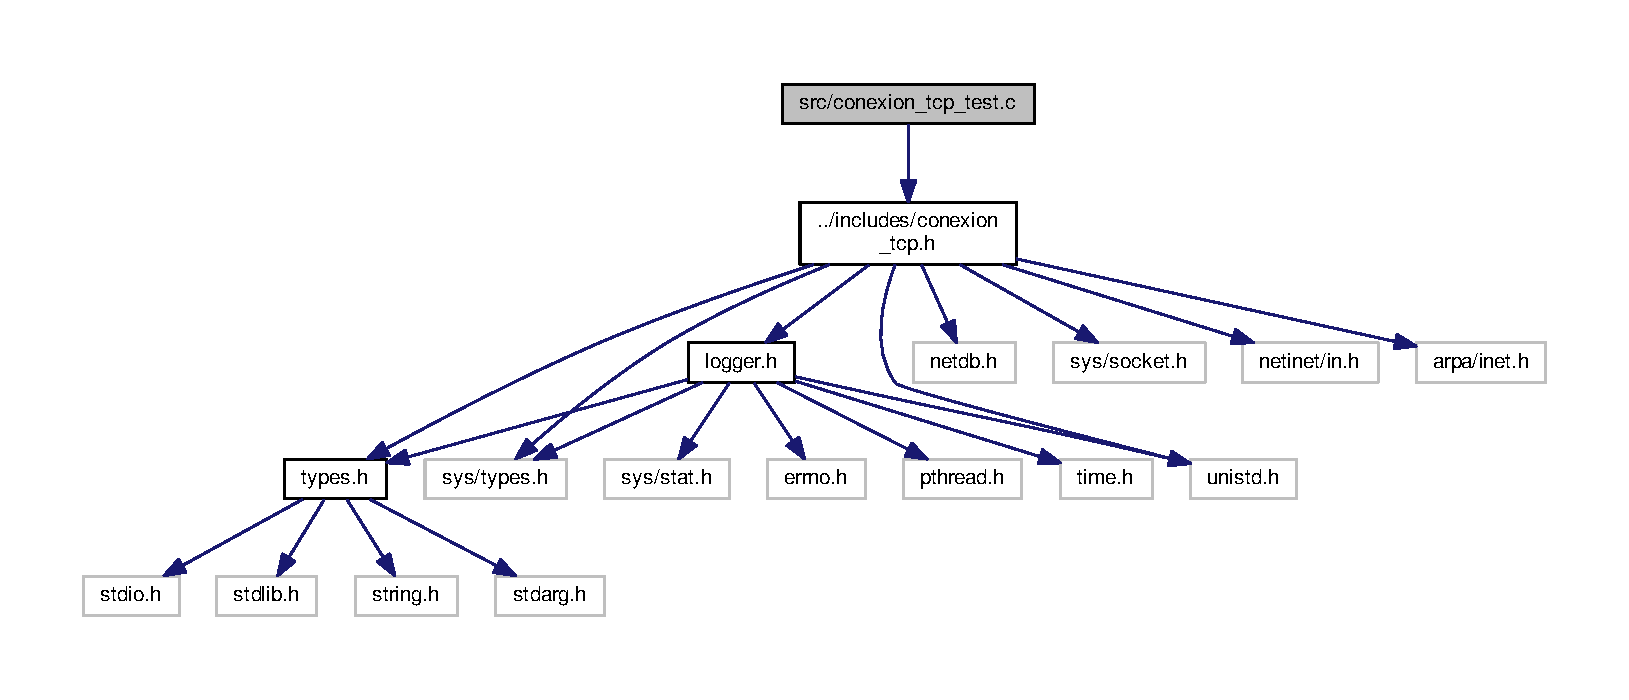
\includegraphics[width=350pt]{conexion__tcp__test_8c__incl}
\end{center}
\end{figure}
\subsection*{Functions}
\begin{DoxyCompactItemize}
\item 
int \hyperlink{conexion__tcp__test_8c_a0ddf1224851353fc92bfbff6f499fa97}{main} (int argc, char $\ast$argv\mbox{[}$\,$\mbox{]})
\end{DoxyCompactItemize}


\subsection{Function Documentation}
\hypertarget{conexion__tcp__test_8c_a0ddf1224851353fc92bfbff6f499fa97}{\index{conexion\-\_\-tcp\-\_\-test.\-c@{conexion\-\_\-tcp\-\_\-test.\-c}!main@{main}}
\index{main@{main}!conexion_tcp_test.c@{conexion\-\_\-tcp\-\_\-test.\-c}}
\subsubsection[{main}]{\setlength{\rightskip}{0pt plus 5cm}int main (
\begin{DoxyParamCaption}
\item[{int}]{argc, }
\item[{char $\ast$}]{argv\mbox{[}$\,$\mbox{]}}
\end{DoxyParamCaption}
)}}\label{conexion__tcp__test_8c_a0ddf1224851353fc92bfbff6f499fa97}

\begin{DoxyCode}
14                                  \{
15 
16         \textcolor{comment}{/* pruebas en el momento durante el desarrollo, nada persistente*/}
17         \textcolor{keywordflow}{return} EXIT\_SUCCESS;
18 \}\end{DoxyCode}

\hypertarget{daemon_8c}{}\section{src/daemon.c File Reference}
\label{daemon_8c}\index{src/daemon.\+c@{src/daemon.\+c}}


Implementacion de las funciones para daemonizar el servidor.  


{\ttfamily \#include \char`\"{}../includes/daemon.\+h\char`\"{}}\\*
Include dependency graph for daemon.\+c\+:
% FIG 0
\subsection*{Functions}
\begin{DoxyCompactItemize}
\item 
int \hyperlink{daemon_8c_ae983f3eb0ff5cebb14c2ae123043df39}{daemonizar} (char $\ast$servicio)
\begin{DoxyCompactList}\small\item\em Funcion para demonizar a un servicio. \end{DoxyCompactList}\end{DoxyCompactItemize}


\subsection{Detailed Description}
Implementacion de las funciones para daemonizar el servidor. 

\begin{DoxyAuthor}{Author}
Alfonso Sebares 

Beatriz de Pablo 
\end{DoxyAuthor}


\subsection{Function Documentation}
\index{daemon.\+c@{daemon.\+c}!daemonizar@{daemonizar}}
\index{daemonizar@{daemonizar}!daemon.\+c@{daemon.\+c}}
\subsubsection[{\texorpdfstring{daemonizar(char $\ast$servicio)}{daemonizar(char *servicio)}}]{\setlength{\rightskip}{0pt plus 5cm}int daemonizar (
\begin{DoxyParamCaption}
\item[{char $\ast$}]{servicio}
\end{DoxyParamCaption}
)}\hypertarget{daemon_8c_ae983f3eb0ff5cebb14c2ae123043df39}{}\label{daemon_8c_ae983f3eb0ff5cebb14c2ae123043df39}


Funcion para demonizar a un servicio. 


\begin{DoxyParams}{Parameters}
{\em char} & $\ast$ servicio\+: Nombre del servidor para dejarlo en segundo plano \\
\hline
\end{DoxyParams}
\begin{DoxyReturn}{Returns}
OK si todo ha salido bien, E\+R\+R\+OR si hay algun fallo 
\end{DoxyReturn}

\begin{DoxyCode}
16                                  \{
17 
18         pid\_t pid;
19         pid\_t sid;
20 
21         \textcolor{keywordflow}{if} (servicio==NULL)\{
22                 syslog(LOG\_ERR, \textcolor{stringliteral}{"Escriba un servicio no nulo."});
23                 \textcolor{keywordflow}{return} \hyperlink{daemon_8h_a8fe83ac76edc595f6b98cd4a4127aed5}{ERROR};
24         \}
25 
26         \textcolor{comment}{/* 1. Ceamos proceso hijo y terminamos el proceso padre */}
27         pid=fork();
28 
29         \textcolor{keywordflow}{if} (pid < 0) \{
30                 syslog(LOG\_ERR, \textcolor{stringliteral}{"Error al crear proceso hijo"});
31                 \textcolor{keywordflow}{return} \hyperlink{daemon_8h_a8fe83ac76edc595f6b98cd4a4127aed5}{ERROR};
32         \}
33         \textcolor{keywordflow}{if} (pid > 0) \{
34                 syslog(LOG\_INFO, \textcolor{stringliteral}{"Liberando al padre"});
35                 \textcolor{keywordflow}{return} \hyperlink{daemon_8h_aba51915c87d64af47fb1cc59348961c9}{OK};
36         \}
37 
38         
39         \textcolor{comment}{/* 2. Crear una nueva sesión de tal forma que el proceso pase a ser lider de sesión, y no sea un
       zombie. */}
40         sid=setsid();
41         \textcolor{keywordflow}{if} (sid < 0) \{
42                 syslog (LOG\_ERR, \textcolor{stringliteral}{"Error creando un SID para el hijo del proceso"});
43                 \textcolor{keywordflow}{return} \hyperlink{daemon_8h_a8fe83ac76edc595f6b98cd4a4127aed5}{ERROR};
44         \}
45 
46         
47         \textcolor{comment}{/* 3. Cambiar la máscara para que los ficheros sean accesibles a cualquiera (0) */}
48         umask (0);
49 
50         \textcolor{comment}{/* 4. Establecer el directorio raíz / como directorio de trabajo */}
51         \textcolor{keywordflow}{if}((chdir(\textcolor{stringliteral}{"/"})) < 0)\{
52                 syslog (LOG\_ERR, \textcolor{stringliteral}{"Error al cambiar el directorio de trabajo a la raíz"});
53                 \textcolor{keywordflow}{return} \hyperlink{daemon_8h_a8fe83ac76edc595f6b98cd4a4127aed5}{ERROR};
54         \}
55 
56         \textcolor{comment}{/* 5. Cerrar todos los descriptores de fichero que pueda haber abiertos ya que no se puede usar la
       terminal*/}
57         syslog(LOG\_INFO, \textcolor{stringliteral}{"Cerrando descriptores"});
58 
59         close(STDIN\_FILENO); 
60         close(STDOUT\_FILENO);
61         close(STDERR\_FILENO);
62 
63         syslog(LOG\_INFO, \textcolor{stringliteral}{"Mandando descriptores a dev/null.."});
64         
65         freopen(\textcolor{stringliteral}{"/dev/null"}, \textcolor{stringliteral}{"r"}, stdin);
66         freopen(\textcolor{stringliteral}{"/dev/null"}, \textcolor{stringliteral}{"w"}, stdout);
67         freopen(\textcolor{stringliteral}{"/dev/null"}, \textcolor{stringliteral}{"w"}, stderr);
68 
69         \textcolor{comment}{/* 6. Abrir el log del sistema para su uso posterior (para que haya comunicacion con el demonio) */}
70         openlog (servicio, LOG\_CONS | LOG\_PID | LOG\_NDELAY, LOG\_LOCAL3);
71 
72         syslog (LOG\_INFO, \textcolor{stringliteral}{"Iniciado nuevo servidor"});
73 
74         \textcolor{keywordflow}{return} \hyperlink{daemon_8h_aba51915c87d64af47fb1cc59348961c9}{OK};
75 \}
\end{DoxyCode}

\hypertarget{echo__client_8c}{\section{src/echo\-\_\-client.c File Reference}
\label{echo__client_8c}\index{src/echo\-\_\-client.\-c@{src/echo\-\_\-client.\-c}}
}


Cliente echo utilizado para aprendizaje y pruebas con sockets.  


{\ttfamily \#include $<$stdio.\-h$>$}\\*
{\ttfamily \#include $<$string.\-h$>$}\\*
{\ttfamily \#include $<$sys/socket.\-h$>$}\\*
{\ttfamily \#include $<$arpa/inet.\-h$>$}\\*
{\ttfamily \#include $<$unistd.\-h$>$}\\*
Include dependency graph for echo\-\_\-client.\-c\-:
\nopagebreak
\begin{figure}[H]
\begin{center}
\leavevmode
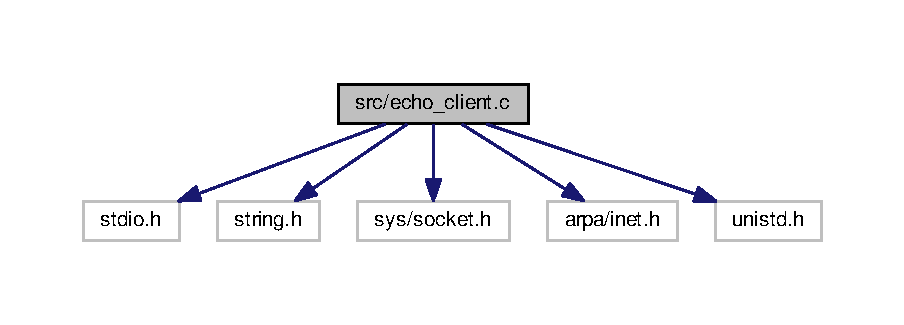
\includegraphics[width=350pt]{echo__client_8c__incl}
\end{center}
\end{figure}
\subsection*{Macros}
\begin{DoxyCompactItemize}
\item 
\#define \hyperlink{echo__client_8c_aeca034f67218340ecb2261a22c2f3dcd}{B\-U\-F\-S\-I\-Z\-E}~1024
\end{DoxyCompactItemize}
\subsection*{Functions}
\begin{DoxyCompactItemize}
\item 
int \hyperlink{echo__client_8c_a0ddf1224851353fc92bfbff6f499fa97}{main} (int argc, char $\ast$argv\mbox{[}$\,$\mbox{]})
\end{DoxyCompactItemize}


\subsection{Detailed Description}
Cliente echo utilizado para aprendizaje y pruebas con sockets. \begin{DoxyAuthor}{Author}
Alfonso Sebares 

Beatriz de Pablo 
\end{DoxyAuthor}
\begin{DoxyDate}{Date}
13/02/17 
\end{DoxyDate}


\subsection{Macro Definition Documentation}
\hypertarget{echo__client_8c_aeca034f67218340ecb2261a22c2f3dcd}{\index{echo\-\_\-client.\-c@{echo\-\_\-client.\-c}!B\-U\-F\-S\-I\-Z\-E@{B\-U\-F\-S\-I\-Z\-E}}
\index{B\-U\-F\-S\-I\-Z\-E@{B\-U\-F\-S\-I\-Z\-E}!echo_client.c@{echo\-\_\-client.\-c}}
\subsubsection[{B\-U\-F\-S\-I\-Z\-E}]{\setlength{\rightskip}{0pt plus 5cm}\#define B\-U\-F\-S\-I\-Z\-E~1024}}\label{echo__client_8c_aeca034f67218340ecb2261a22c2f3dcd}


\subsection{Function Documentation}
\hypertarget{echo__client_8c_a0ddf1224851353fc92bfbff6f499fa97}{\index{echo\-\_\-client.\-c@{echo\-\_\-client.\-c}!main@{main}}
\index{main@{main}!echo_client.c@{echo\-\_\-client.\-c}}
\subsubsection[{main}]{\setlength{\rightskip}{0pt plus 5cm}int main (
\begin{DoxyParamCaption}
\item[{int}]{argc, }
\item[{char $\ast$}]{argv\mbox{[}$\,$\mbox{]}}
\end{DoxyParamCaption}
)}}\label{echo__client_8c_a0ddf1224851353fc92bfbff6f499fa97}

\begin{DoxyCode}
19 \{
20     \textcolor{keywordtype}{int} sock;
21     \textcolor{keyword}{struct }sockaddr\_in server;
22     \textcolor{keywordtype}{char} message[\hyperlink{echo__client_8c_aeca034f67218340ecb2261a22c2f3dcd}{BUFSIZE}] , server\_reply[\hyperlink{echo__client_8c_aeca034f67218340ecb2261a22c2f3dcd}{BUFSIZE}];
23      
24     \textcolor{comment}{//Create socket}
25     sock = socket(AF\_INET , SOCK\_STREAM , 0);
26     \textcolor{keywordflow}{if} (sock == -1)
27     \{
28         printf(\textcolor{stringliteral}{"Could not create socket"});
29     \}
30     puts(\textcolor{stringliteral}{"Socket created"});
31      
32     server.sin\_addr.s\_addr = inet\_addr(\textcolor{stringliteral}{"127.0.0.1"});
33     server.sin\_family = AF\_INET;
34     server.sin\_port = htons( 8888 );
35  
36     \textcolor{comment}{//Connect to remote server}
37     \textcolor{keywordflow}{if} (connect(sock , (\textcolor{keyword}{struct} sockaddr *)&server , \textcolor{keyword}{sizeof}(server)) < 0)
38     \{
39         perror(\textcolor{stringliteral}{"connect failed. Error"});
40         \textcolor{keywordflow}{return} 1;
41     \}
42      
43     puts(\textcolor{stringliteral}{"Connected\(\backslash\)n"});
44      
45     \textcolor{comment}{//keep communicating with server}
46     \textcolor{keywordflow}{while}((strcmp(message, \textcolor{stringliteral}{"\_STOP\_"}) != 0))
47     \{
48         printf(\textcolor{stringliteral}{"Enter message : "});
49         scanf(\textcolor{stringliteral}{"%s"} , message);
50 
51         \textcolor{comment}{//Send some data}
52         \textcolor{keywordflow}{if}( send(sock , message , \textcolor{keyword}{sizeof}(message) , 0) < 0)
53         \{
54             puts(\textcolor{stringliteral}{"Send failed"});
55             \textcolor{keywordflow}{return} 1;
56         \}
57          
58         \textcolor{comment}{//Receive a reply from the server}
59         \textcolor{keywordflow}{if}( recv(sock , server\_reply , \hyperlink{echo__client_8c_aeca034f67218340ecb2261a22c2f3dcd}{BUFSIZE} , 0) < 0)
60         \{
61             puts(\textcolor{stringliteral}{"recv failed"});
62             \textcolor{keywordflow}{break};
63         \}
64          
65         puts(\textcolor{stringliteral}{"Server reply :"});
66         puts(server\_reply);
67     \}
68      
69     puts(\textcolor{stringliteral}{"\_STOP\_ enviado, cerrar conexion"});
70     close(sock);
71     \textcolor{keywordflow}{return} 0;
72 \}\end{DoxyCode}

\hypertarget{echo__server_8c}{}\section{src/echo\+\_\+server.c File Reference}
\label{echo__server_8c}\index{src/echo\+\_\+server.\+c@{src/echo\+\_\+server.\+c}}


Servidor echo utilizado para comprender y desarrollar el servidor I\+RC.  


{\ttfamily \#include $<$stdio.\+h$>$}\\*
{\ttfamily \#include $<$unistd.\+h$>$}\\*
{\ttfamily \#include $<$stdlib.\+h$>$}\\*
{\ttfamily \#include $<$string.\+h$>$}\\*
{\ttfamily \#include $<$netdb.\+h$>$}\\*
{\ttfamily \#include $<$sys/types.\+h$>$}\\*
{\ttfamily \#include $<$sys/socket.\+h$>$}\\*
{\ttfamily \#include $<$netinet/in.\+h$>$}\\*
{\ttfamily \#include $<$arpa/inet.\+h$>$}\\*
{\ttfamily \#include $<$pthread.\+h$>$}\\*
{\ttfamily \#include $<$errno.\+h$>$}\\*
Include dependency graph for echo\+\_\+server.\+c\+:
% FIG 0
\subsection*{Macros}
\begin{DoxyCompactItemize}
\item 
\#define \hyperlink{echo__server_8c_aeca034f67218340ecb2261a22c2f3dcd}{B\+U\+F\+S\+I\+ZE}~1024
\item 
\#define \hyperlink{echo__server_8c_a3e4b4faa36cc9e3a7d9895aec8f27592}{M\+A\+X\+\_\+\+C\+O\+N\+\_\+\+R\+EQ}~10
\end{DoxyCompactItemize}
\subsection*{Functions}
\begin{DoxyCompactItemize}
\item 
void \hyperlink{echo__server_8c_aad9796c174f7ef5d226cd169f2520fd5}{error} (char $\ast$\hyperlink{_g-2361-06-_p1-_server_8c_a32d2f5216cddb59c7cc8fb2806a7e727}{msg})
\item 
int \hyperlink{echo__server_8c_a0ddf1224851353fc92bfbff6f499fa97}{main} (int argc, char $\ast$argv\mbox{[}$\,$\mbox{]})
\end{DoxyCompactItemize}


\subsection{Detailed Description}
Servidor echo utilizado para comprender y desarrollar el servidor I\+RC. 

Servidor echo utilizado para comprender y desarrollar el servidor I\+RC con protocolo S\+SL.

\begin{DoxyAuthor}{Author}
Alfonso Sebares 

Beatriz de Pablo

Alfonso Sebares 

Beatriz de Pablo 

Celia Mateos

Alfonso Sebares 

Beatriz de Pablo 

Celia Mateos 
\end{DoxyAuthor}
\begin{DoxyDate}{Date}
28/04/17 
\end{DoxyDate}


\subsection{Macro Definition Documentation}
\index{echo\+\_\+server.\+c@{echo\+\_\+server.\+c}!B\+U\+F\+S\+I\+ZE@{B\+U\+F\+S\+I\+ZE}}
\index{B\+U\+F\+S\+I\+ZE@{B\+U\+F\+S\+I\+ZE}!echo\+\_\+server.\+c@{echo\+\_\+server.\+c}}
\subsubsection[{\texorpdfstring{B\+U\+F\+S\+I\+ZE}{BUFSIZE}}]{\setlength{\rightskip}{0pt plus 5cm}\#define B\+U\+F\+S\+I\+ZE~1024}\hypertarget{echo__server_8c_aeca034f67218340ecb2261a22c2f3dcd}{}\label{echo__server_8c_aeca034f67218340ecb2261a22c2f3dcd}
Tam. max. del buffer que se lee \index{echo\+\_\+server.\+c@{echo\+\_\+server.\+c}!M\+A\+X\+\_\+\+C\+O\+N\+\_\+\+R\+EQ@{M\+A\+X\+\_\+\+C\+O\+N\+\_\+\+R\+EQ}}
\index{M\+A\+X\+\_\+\+C\+O\+N\+\_\+\+R\+EQ@{M\+A\+X\+\_\+\+C\+O\+N\+\_\+\+R\+EQ}!echo\+\_\+server.\+c@{echo\+\_\+server.\+c}}
\subsubsection[{\texorpdfstring{M\+A\+X\+\_\+\+C\+O\+N\+\_\+\+R\+EQ}{MAX_CON_REQ}}]{\setlength{\rightskip}{0pt plus 5cm}\#define M\+A\+X\+\_\+\+C\+O\+N\+\_\+\+R\+EQ~10}\hypertarget{echo__server_8c_a3e4b4faa36cc9e3a7d9895aec8f27592}{}\label{echo__server_8c_a3e4b4faa36cc9e3a7d9895aec8f27592}
Max. de peticiones de conexion activas (e.\+g. la 11 falla si puesto a 10) 

\subsection{Function Documentation}
\index{echo\+\_\+server.\+c@{echo\+\_\+server.\+c}!error@{error}}
\index{error@{error}!echo\+\_\+server.\+c@{echo\+\_\+server.\+c}}
\subsubsection[{\texorpdfstring{error(char $\ast$msg)}{error(char *msg)}}]{\setlength{\rightskip}{0pt plus 5cm}void error (
\begin{DoxyParamCaption}
\item[{char $\ast$}]{msg}
\end{DoxyParamCaption}
)}\hypertarget{echo__server_8c_aad9796c174f7ef5d226cd169f2520fd5}{}\label{echo__server_8c_aad9796c174f7ef5d226cd169f2520fd5}

\begin{DoxyCode}
24                       \{
25         perror(\hyperlink{_g-2361-06-_p1-_server_8c_a32d2f5216cddb59c7cc8fb2806a7e727}{msg});
26         exit(1);
27 \}
\end{DoxyCode}
\index{echo\+\_\+server.\+c@{echo\+\_\+server.\+c}!main@{main}}
\index{main@{main}!echo\+\_\+server.\+c@{echo\+\_\+server.\+c}}
\subsubsection[{\texorpdfstring{main(int argc, char $\ast$argv[])}{main(int argc, char *argv[])}}]{\setlength{\rightskip}{0pt plus 5cm}int main (
\begin{DoxyParamCaption}
\item[{int}]{argc, }
\item[{char $\ast$}]{argv\mbox{[}$\,$\mbox{]}}
\end{DoxyParamCaption}
)}\hypertarget{echo__server_8c_a0ddf1224851353fc92bfbff6f499fa97}{}\label{echo__server_8c_a0ddf1224851353fc92bfbff6f499fa97}

\begin{DoxyCode}
30 \{
31         \textcolor{keywordtype}{int} socket\_desc , client\_sock , c , read\_size;
32         \textcolor{keywordtype}{int} portno;
33         \textcolor{keywordtype}{int} optval; \textcolor{comment}{/* flag value for setsockopt */}
34         \textcolor{keyword}{struct }sockaddr\_in server , client;
35         \textcolor{keyword}{struct }hostent *hostp; \textcolor{comment}{/* client host info */}
36         \textcolor{keywordtype}{char} client\_message[\hyperlink{echo__server_8c_aeca034f67218340ecb2261a22c2f3dcd}{BUFSIZE}];
37         \textcolor{keywordtype}{char} *hostaddrp; \textcolor{comment}{/* dotted decimal host addr string */}
38          
39         \textcolor{keywordflow}{if} (argc != 2) \{
40                 fprintf(stderr, \textcolor{stringliteral}{"usage: %s <port>\(\backslash\)n"}, argv[0]);
41                 exit(1);
42         \}
43         portno = atoi(argv[1]);
44         
45         \textcolor{comment}{//Create socket}
46         socket\_desc = socket(AF\_INET , SOCK\_STREAM , 0);
47         \textcolor{keywordflow}{if} (socket\_desc == -1)
48         \{
49                 printf(\textcolor{stringliteral}{"Could not create socket"});
50         \}
51         puts(\textcolor{stringliteral}{"Socket created"});
52         
53         optval = 1;
54         setsockopt(socket\_desc, SOL\_SOCKET, SO\_REUSEADDR, (\textcolor{keyword}{const} \textcolor{keywordtype}{void} *)&optval , \textcolor{keyword}{sizeof}(\textcolor{keywordtype}{int}));
55 
56         \textcolor{comment}{//Prepare the sockaddr\_in structure}
57         memset((\textcolor{keywordtype}{char} *) &server, 0, \textcolor{keyword}{sizeof}(server));
58         server.sin\_family = AF\_INET;
59         server.sin\_addr.s\_addr = INADDR\_ANY;
60         server.sin\_port = htons((\textcolor{keywordtype}{unsigned} \textcolor{keywordtype}{short})portno );
61          
62         \textcolor{comment}{//Bind}
63         \textcolor{keywordflow}{if}( bind(socket\_desc,(\textcolor{keyword}{struct} sockaddr *)&server , \textcolor{keyword}{sizeof}(server)) < 0)
64         \{
65                 \textcolor{comment}{//print the error message}
66                 \textcolor{comment}{//printf("\(\backslash\)nstrerror: %s\(\backslash\)n", strerror(errno));}
67                 perror(\textcolor{stringliteral}{"bind failed. Error"});
68                 \textcolor{keywordflow}{return} 1;
69         \}
70         puts(\textcolor{stringliteral}{"bind done"});
71          
72         \textcolor{comment}{//Listen}
73         listen(socket\_desc , \hyperlink{echo__server_8c_a3e4b4faa36cc9e3a7d9895aec8f27592}{MAX\_CON\_REQ});
74          
75         \textcolor{comment}{//Accept and incoming connection}
76         puts(\textcolor{stringliteral}{"Waiting for incoming connections..."});
77         c = \textcolor{keyword}{sizeof}(\textcolor{keyword}{struct }sockaddr\_in);
78          
79         \textcolor{comment}{//accept connection from an incoming client}
80         client\_sock = accept(socket\_desc, (\textcolor{keyword}{struct} sockaddr *)&client, (socklen\_t*)&c);
81         \textcolor{keywordflow}{if} (client\_sock < 0)
82         \{
83                 perror(\textcolor{stringliteral}{"accept failed"});
84                 \textcolor{keywordflow}{return} 1;
85         \}
86 
87         hostp = gethostbyaddr((\textcolor{keyword}{const} \textcolor{keywordtype}{char} *)&client.sin\_addr.s\_addr, \textcolor{keyword}{sizeof}(client.sin\_addr.s\_addr), 
      AF\_INET);
88         \textcolor{keywordflow}{if} (hostp == NULL)
89                 \hyperlink{echo__server_8c_aad9796c174f7ef5d226cd169f2520fd5}{error}(\textcolor{stringliteral}{"ERROR on gethostbyaddr"});
90 
91         hostaddrp = inet\_ntoa(client.sin\_addr);
92 
93         \textcolor{keywordflow}{if} (hostaddrp == NULL)
94                 \hyperlink{echo__server_8c_aad9796c174f7ef5d226cd169f2520fd5}{error}(\textcolor{stringliteral}{"ERROR on inet\_ntoa\(\backslash\)n"});
95         printf(\textcolor{stringliteral}{"\(\backslash\)nserver established connection with %s (%s)\(\backslash\)n"}, hostp->h\_name, hostaddrp);
96          
97         \textcolor{comment}{//Receive a message from client}
98         \textcolor{keywordflow}{while}( strcmp(client\_message, \textcolor{stringliteral}{"\_STOP\_"}) != 0 )
99         \{
100                 read\_size = recv(client\_sock , client\_message , \hyperlink{echo__server_8c_aeca034f67218340ecb2261a22c2f3dcd}{BUFSIZE} , 0);
101                 printf(\textcolor{stringliteral}{"\(\backslash\)nRecibido: %s"}, client\_message);
102                 \textcolor{keywordflow}{if} (read\_size < 0)\{
103                         perror(\textcolor{stringliteral}{"recv failed"});
104                 \}
105                 \textcolor{comment}{//Send the message back to client}
106                 \textcolor{comment}{//write(client\_sock , client\_message , read\_size);}
107                 \textcolor{comment}{/*afinar un poco mas que mandar siempre BUFSIZE:*/}
108                 write(client\_sock , client\_message , strlen(client\_message)+1); 
109         \}
110         
111         puts(\textcolor{stringliteral}{"Client disconnected"});
112         fflush(stdout);
113         close(client\_sock);
114          
115         \textcolor{keywordflow}{return} 0;
116 \}\end{DoxyCode}


Here is the call graph for this function\+:
% FIG 1



\hypertarget{log__test_8c}{}\section{src/log\+\_\+test.c File Reference}
\label{log__test_8c}\index{src/log\+\_\+test.\+c@{src/log\+\_\+test.\+c}}


Prueba de la libreria de logs.  


{\ttfamily \#include \char`\"{}../includes/logger.\+h\char`\"{}}\\*
Include dependency graph for log\+\_\+test.\+c\+:
% FIG 0
\subsection*{Functions}
\begin{DoxyCompactItemize}
\item 
int \hyperlink{log__test_8c_ae66f6b31b5ad750f1fe042a706a4e3d4}{main} ()
\end{DoxyCompactItemize}
\subsection*{Variables}
\begin{DoxyCompactItemize}
\item 
pthread\+\_\+mutex\+\_\+t \hyperlink{log__test_8c_a53497b00bd1ff0270ca7a108d5794dbc}{loglock}
\begin{DoxyCompactList}\small\item\em Definicion del Mutex para el descriptor de fichero del log. \end{DoxyCompactList}\end{DoxyCompactItemize}


\subsection{Detailed Description}
Prueba de la libreria de logs. 

\begin{DoxyAuthor}{Author}
Alfonso Sebares 

Beatriz de Pablo 
\end{DoxyAuthor}
\begin{DoxyDate}{Date}
13/02/17 
\end{DoxyDate}


\subsection{Function Documentation}
\index{log\+\_\+test.\+c@{log\+\_\+test.\+c}!main@{main}}
\index{main@{main}!log\+\_\+test.\+c@{log\+\_\+test.\+c}}
\subsubsection[{\texorpdfstring{main()}{main()}}]{\setlength{\rightskip}{0pt plus 5cm}int main (
\begin{DoxyParamCaption}
{}
\end{DoxyParamCaption}
)}\hypertarget{log__test_8c_ae66f6b31b5ad750f1fe042a706a4e3d4}{}\label{log__test_8c_ae66f6b31b5ad750f1fe042a706a4e3d4}

\begin{DoxyCode}
18 \{
19    FILE* fp = NULL;
20    fp = \hyperlink{logger_8h_a1fa2e9d39664def63d53e3d576dc923f}{initLog}();
21 
22    \textcolor{keywordflow}{if} (pthread\_mutex\_init(&\hyperlink{log__test_8c_a53497b00bd1ff0270ca7a108d5794dbc}{loglock}, NULL) != \hyperlink{daemon_8h_aba51915c87d64af47fb1cc59348961c9}{OK})\{
23       perror(\textcolor{stringliteral}{"\(\backslash\)n mutex init ha devuelto error\(\backslash\)n"});
24       \textcolor{keywordflow}{return} EXIT\_FAILURE;
25    \}
26 
27    \textcolor{keywordflow}{if} (fp == NULL)\{
28       perror(\textcolor{stringliteral}{"ERR abriendo fichero"});
29       \textcolor{keywordflow}{return} (EXIT\_FAILURE);
30    \}
31 
32    \hyperlink{logger_8h_af71188329ee1cf68a59d3f9ddd035ca6}{logEvent}(\textcolor{stringliteral}{"Evento 1..."});
33    \hyperlink{logger_8h_af71188329ee1cf68a59d3f9ddd035ca6}{logEvent}(\textcolor{stringliteral}{"Evento 2..."});
34    \hyperlink{logger_8h_af71188329ee1cf68a59d3f9ddd035ca6}{logEvent}(\textcolor{stringliteral}{"Evento 3..."});
35    \hyperlink{logger_8h_af71188329ee1cf68a59d3f9ddd035ca6}{logEvent}(\textcolor{stringliteral}{"Gatos :3"});
36 
37    fp = fopen(\textcolor{stringliteral}{"fichero-inexistente.txt"}, \textcolor{stringliteral}{"r"});
38    \textcolor{keywordflow}{if} (fp == NULL)\{
39       \hyperlink{logger_8h_a9487660b2ec318326782a9d9e32f8461}{logERR}(\textcolor{stringliteral}{"Error de fopen detectado"});
40    \}
41 
42    pthread\_mutex\_destroy(&\hyperlink{log__test_8c_a53497b00bd1ff0270ca7a108d5794dbc}{loglock});
43    \textcolor{keywordflow}{return} (EXIT\_SUCCESS);
44 \}\end{DoxyCode}


Here is the call graph for this function\+:
% FIG 1




\subsection{Variable Documentation}
\index{log\+\_\+test.\+c@{log\+\_\+test.\+c}!loglock@{loglock}}
\index{loglock@{loglock}!log\+\_\+test.\+c@{log\+\_\+test.\+c}}
\subsubsection[{\texorpdfstring{loglock}{loglock}}]{\setlength{\rightskip}{0pt plus 5cm}pthread\+\_\+mutex\+\_\+t loglock}\hypertarget{log__test_8c_a53497b00bd1ff0270ca7a108d5794dbc}{}\label{log__test_8c_a53497b00bd1ff0270ca7a108d5794dbc}


Definicion del Mutex para el descriptor de fichero del log. 

Declaracion del Mutex para el descriptor de fichero del log. Siempre tiene que ser definida en el source princpal. 
\hypertarget{xchat2_8c}{\section{src/xchat2.c File Reference}
\label{xchat2_8c}\index{src/xchat2.\-c@{src/xchat2.\-c}}
}


Fichero con principalmente la implementación de los callbacks de xchat2.  


{\ttfamily \#include \char`\"{}../includes/xchat2.\-h\char`\"{}}\\*
Include dependency graph for xchat2.\-c\-:
\nopagebreak
\begin{figure}[H]
\begin{center}
\leavevmode
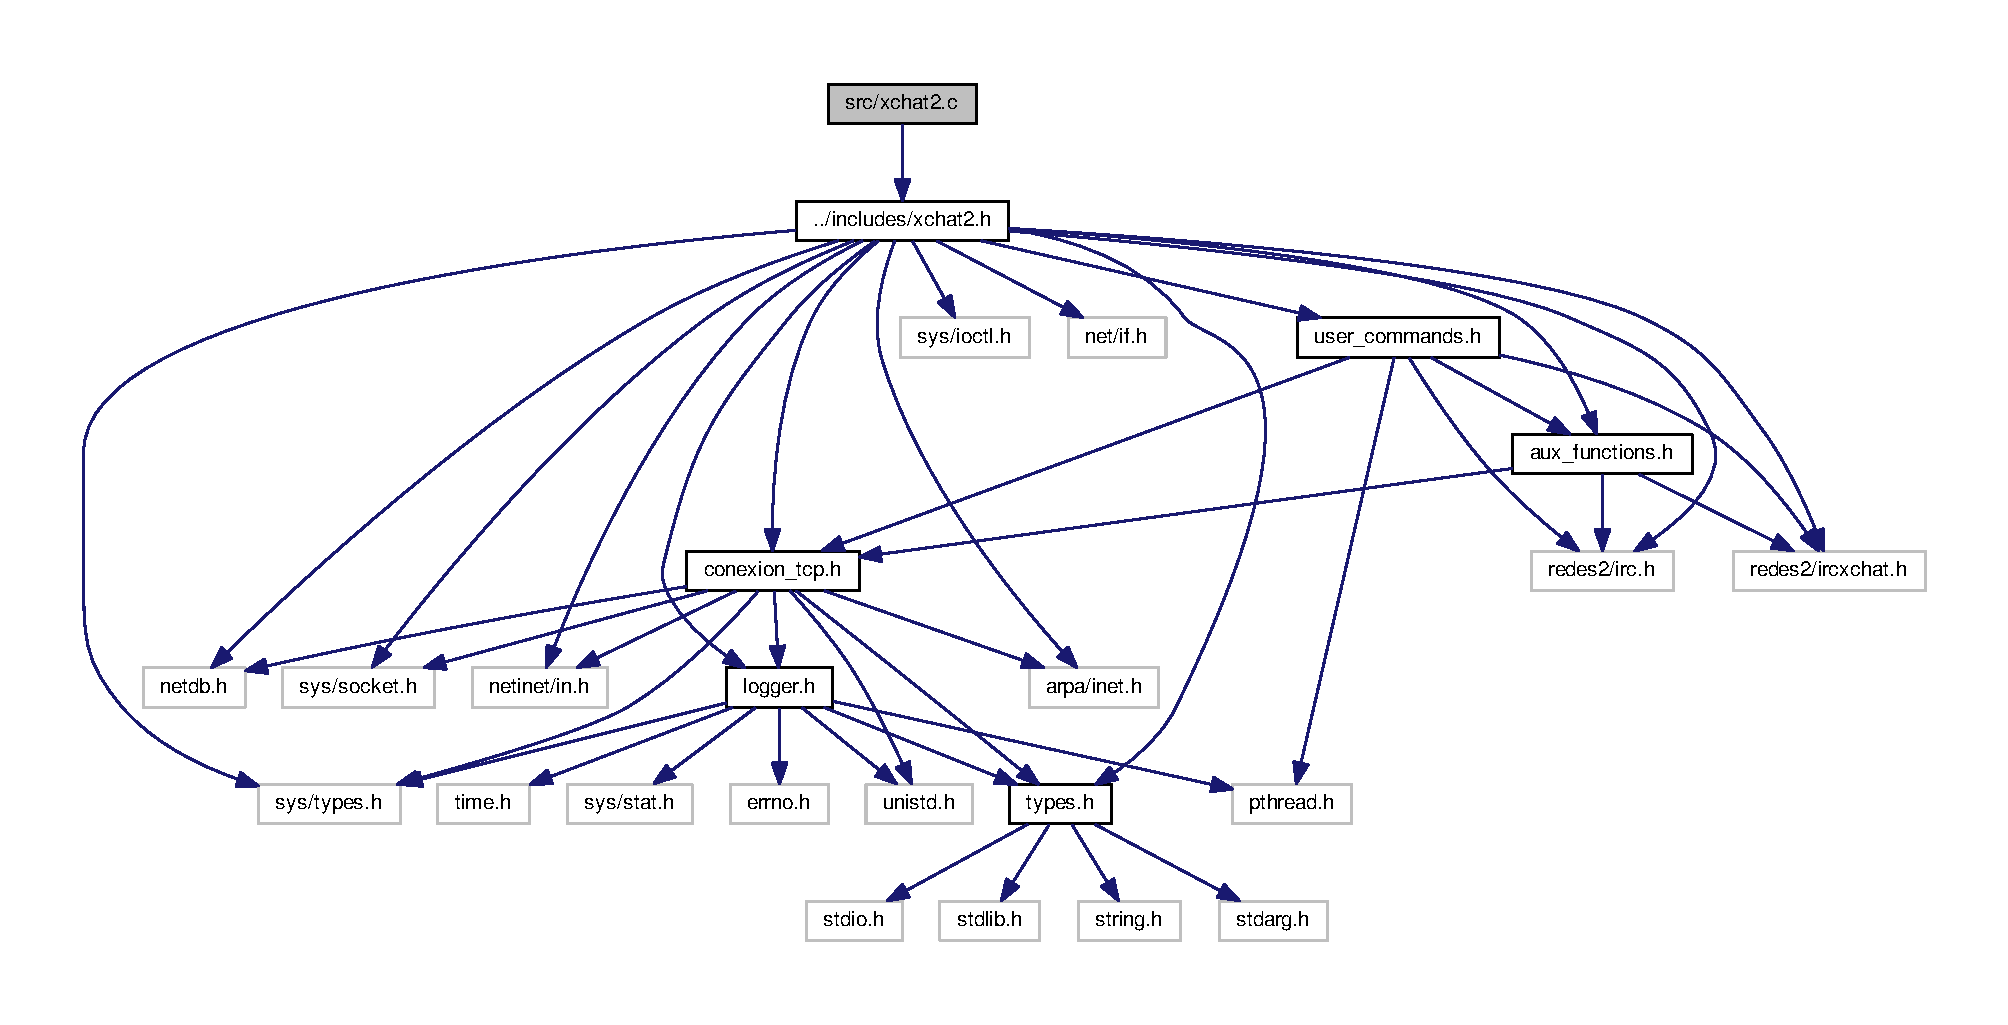
\includegraphics[width=350pt]{xchat2_8c__incl}
\end{center}
\end{figure}
\subsection*{Functions}
\begin{DoxyCompactItemize}
\item 
int \hyperlink{xchat2_8c_a41f93f364aea303a0c93177289733f92}{command\-\_\-query} (char $\ast$message)
\begin{DoxyCompactList}\small\item\em Parsea los mensajes y respuestas que recibe del servidor. \end{DoxyCompactList}\item 
void \hyperlink{xchat2_8c_a98484e1bbb136d37503aa6c604eff6a2}{glue\-And\-Query} (char $\ast$command, char $\ast$\hyperlink{xchat2_8c_a4e304440b657a8d3265793203cb12393}{last\-\_\-command})
\item 
void \hyperlink{xchat2_8c_a63f7dc08db4a2318cb526eee804709b3}{unpipe} (char $\ast$message, int M\-A\-X\-D\-A\-T\-A\-\_\-flag)
\begin{DoxyCompactList}\small\item\em Funcion para dividir en comandos la cadena \char`\"{}message\char`\"{}. \end{DoxyCompactList}\item 
void \hyperlink{xchat2_8c_a7230d43b8458797c679e7180bf1fda90}{receive\-\_\-messages} (void $\ast$no\-\_\-arg)
\begin{DoxyCompactList}\small\item\em Funcion ejecutada por un hilo, que recibe mensajes del servidor y los procesa segun el tipo de respuesta. \end{DoxyCompactList}\item 
void \hyperlink{xchat2_8c_a33f80a29a744e4182b29e23f13c1f05c}{I\-R\-C\-Interface\-\_\-\-Activate\-Channel\-Key} (char $\ast$channel, char $\ast$key)
\item 
void \hyperlink{xchat2_8c_a7a439929c246e342ae525139b2c39f5d}{I\-R\-C\-Interface\-\_\-\-Activate\-External\-Messages} (char $\ast$channel)
\item 
void \hyperlink{xchat2_8c_ac72762ab1e3575b421b967241db23f9c}{I\-R\-C\-Interface\-\_\-\-Activate\-Invite} (char $\ast$channel)
\item 
void \hyperlink{xchat2_8c_af83498f4058311f4562c43a9b70566b2}{I\-R\-C\-Interface\-\_\-\-Activate\-Moderated} (char $\ast$channel)
\item 
void \hyperlink{xchat2_8c_ab5694cc413472173bfcaa969c7d9800e}{I\-R\-C\-Interface\-\_\-\-Activate\-Nicks\-Limit} (char $\ast$channel, int limit)
\item 
void \hyperlink{xchat2_8c_ab1f09c737c7c109a97e22de6072d731d}{I\-R\-C\-Interface\-\_\-\-Activate\-Private} (char $\ast$channel)
\item 
void \hyperlink{xchat2_8c_ac45f12d4dcacf3b5485eec6fdc51df93}{I\-R\-C\-Interface\-\_\-\-Activate\-Protect\-Topic} (char $\ast$channel)
\item 
void \hyperlink{xchat2_8c_aa9e9155115b834d85a4d10cb27f99093}{I\-R\-C\-Interface\-\_\-\-Activate\-Secret} (char $\ast$channel)
\item 
void \hyperlink{xchat2_8c_a42773b5a840f9d0455f148d285e1e595}{I\-R\-C\-Interface\-\_\-\-Ban\-Nick} (char $\ast$channel, char $\ast$nick)
\item 
long \hyperlink{xchat2_8c_aed072f4ce0d6e90697d4d6eb0278a2ad}{I\-R\-C\-Interface\-\_\-\-Connect} (char $\ast$nick, char $\ast$user, char $\ast$realname, char $\ast$password, char $\ast$server, int port, boolean ssl)
\item 
void \hyperlink{xchat2_8c_a3e67ee0cd384b524d57fda14593dce8e}{I\-R\-C\-Interface\-\_\-\-Deactivate\-Channel\-Key} (char $\ast$channel)
\item 
void \hyperlink{xchat2_8c_a638b1535f4ecbc9a6affb2df2a6a946e}{I\-R\-C\-Interface\-\_\-\-Deactivate\-External\-Messages} (char $\ast$channel)
\item 
void \hyperlink{xchat2_8c_a9ba4e98a3729737aa63ebec54ba4e894}{I\-R\-C\-Interface\-\_\-\-Deactivate\-Invite} (char $\ast$channel)
\item 
void \hyperlink{xchat2_8c_ab760e8144b38f6c14bd809d157cee5d4}{I\-R\-C\-Interface\-\_\-\-Deactivate\-Moderated} (char $\ast$channel)
\item 
void \hyperlink{xchat2_8c_a92c8cfbe2e14e19277e1c97d11719e80}{I\-R\-C\-Interface\-\_\-\-Deactivate\-Nicks\-Limit} (char $\ast$channel)
\item 
void \hyperlink{xchat2_8c_a8a6141803691ba327f11ba763ad075d4}{I\-R\-C\-Interface\-\_\-\-Deactivate\-Private} (char $\ast$channel)
\item 
void \hyperlink{xchat2_8c_a5a57541a950f8c2c40b4b44c32b28ed9}{I\-R\-C\-Interface\-\_\-\-Deactivate\-Protect\-Topic} (char $\ast$channel)
\item 
void \hyperlink{xchat2_8c_a4956427664cabc7d5b2bd1589a207324}{I\-R\-C\-Interface\-\_\-\-Deactivate\-Secret} (char $\ast$channel)
\item 
boolean \hyperlink{xchat2_8c_a8bf0424ef7f845be79a056e9aed56fe2}{I\-R\-C\-Interface\-\_\-\-Disconnect\-Server} (char $\ast$server, int port)
\item 
boolean \hyperlink{xchat2_8c_ab431412191716f751461f94d613ffdab}{I\-R\-C\-Interface\-\_\-\-Exit\-Audio\-Chat} (char $\ast$nick)
\item 
void \hyperlink{xchat2_8c_ae075029bb55e8b995f22beb0810674f4}{I\-R\-C\-Interface\-\_\-\-Give\-Op} (char $\ast$channel, char $\ast$nick)
\item 
void \hyperlink{xchat2_8c_ae9effb4bdaf4a2cdf2dd9edbeb90b430}{I\-R\-C\-Interface\-\_\-\-Give\-Voice} (char $\ast$channel, char $\ast$nick)
\item 
void \hyperlink{xchat2_8c_a7adfea400a96160585f86179bafb055f}{I\-R\-C\-Interface\-\_\-\-Kick\-Nick} (char $\ast$channel, char $\ast$nick)
\item 
void \hyperlink{xchat2_8c_a214e10b19c8be028fb35d2a7abf3f798}{I\-R\-C\-Interface\-\_\-\-New\-Command\-Text} (char $\ast$command)
\item 
void \hyperlink{xchat2_8c_a080cf34ff506481737f6d08af60ca92b}{I\-R\-C\-Interface\-\_\-\-New\-Topic\-Enter} (char $\ast$topicdata)
\item 
boolean \hyperlink{xchat2_8c_a100f1c87bb3b399a7284e62dd2e6172a}{I\-R\-C\-Interface\-\_\-\-Send\-File} (char $\ast$filename, char $\ast$nick, char $\ast$data, long unsigned int length)
\item 
boolean \hyperlink{xchat2_8c_a5dc7a44587e609b416a783cd420a12e3}{I\-R\-C\-Interface\-\_\-\-Start\-Audio\-Chat} (char $\ast$nick)
\item 
boolean \hyperlink{xchat2_8c_a754a3d3dd311194637c07cc701e7d507}{I\-R\-C\-Interface\-\_\-\-Stop\-Audio\-Chat} (char $\ast$nick)
\item 
void \hyperlink{xchat2_8c_a4e2a1ea75e59306142030a91a054b7e6}{I\-R\-C\-Interface\-\_\-\-Take\-Op} (char $\ast$channel, char $\ast$nick)
\item 
void \hyperlink{xchat2_8c_a2ff2e10ed1cb1a399293b6f76ac1e5ae}{I\-R\-C\-Interface\-\_\-\-Take\-Voice} (char $\ast$channel, char $\ast$nick)
\item 
int \hyperlink{xchat2_8c_a0ddf1224851353fc92bfbff6f499fa97}{main} (int argc, char $\ast$argv\mbox{[}$\,$\mbox{]})
\end{DoxyCompactItemize}
\subsection*{Variables}
\begin{DoxyCompactItemize}
\item 
pthread\-\_\-mutex\-\_\-t \hyperlink{xchat2_8c_a53497b00bd1ff0270ca7a108d5794dbc}{loglock}
\begin{DoxyCompactList}\small\item\em Declaracion del Mutex para el descriptor de fichero del log. Siempre tiene que ser definida en el source princpal. \end{DoxyCompactList}\item 
pthread\-\_\-t \hyperlink{xchat2_8c_ab5efd1efa144e252f4c5312ae57bea2e}{recv\-\_\-tid}
\item 
pthread\-\_\-t \hyperlink{xchat2_8c_a808d33eb5e54db312802ea4b22189ef3}{sendf\-\_\-tid}
\item 
int \hyperlink{xchat2_8c_acd63fb8dbd9439219e2db08dfc173aa0}{sockfd\-\_\-user} = -\/1
\item 
char \hyperlink{xchat2_8c_a7e2f32e47f3780a66e19651d8e79bced}{nick\-\_\-user} \mbox{[}\hyperlink{types_8h_ae7e715c270481406658bbd2bafa2897f}{M\-A\-X\-D\-A\-T\-A}\mbox{]} = \{0\}
\item 
char $\ast$ \hyperlink{xchat2_8c_af203df082d5c6dcaa0c88b07cf86466d}{hostname}
\item 
char $\ast$ \hyperlink{xchat2_8c_a568595cf14231c912fd7ab15a324bd16}{active\-\_\-channel} = N\-U\-L\-L
\item 
char $\ast$ \hyperlink{xchat2_8c_a98d1a6f1c3b6a02b439ca0b9e8434420}{stream}
\item 
char \hyperlink{xchat2_8c_a738cdcabc13fa13e8263986fe5d0fc28}{host\-\_\-name} \mbox{[}128\mbox{]}
\item 
char \hyperlink{xchat2_8c_a4e304440b657a8d3265793203cb12393}{last\-\_\-command} \mbox{[}256\mbox{]} = \char`\"{}\char`\"{}
\item 
int \hyperlink{xchat2_8c_ad1d1f3c86702bf2ea990065ad3293d10}{check\-\_\-next\-\_\-unpipe} = 0
\item 
int \hyperlink{xchat2_8c_a7872bff8c54fa63dccefb6916f983928}{last\-\_\-test} = \hyperlink{types_8h_aba51915c87d64af47fb1cc59348961c9}{O\-K}
\end{DoxyCompactItemize}


\subsection{Detailed Description}
Fichero con principalmente la implementación de los callbacks de xchat2. \begin{DoxyAuthor}{Author}
Alfonso Sebares 

Beatriz de Pablo 

Celia Mateos 
\end{DoxyAuthor}
\begin{DoxyDate}{Date}
20/03/17 
\end{DoxyDate}


\subsection{Function Documentation}
\hypertarget{xchat2_8c_a41f93f364aea303a0c93177289733f92}{\index{xchat2.\-c@{xchat2.\-c}!command\-\_\-query@{command\-\_\-query}}
\index{command\-\_\-query@{command\-\_\-query}!xchat2.c@{xchat2.\-c}}
\subsubsection[{command\-\_\-query}]{\setlength{\rightskip}{0pt plus 5cm}int command\-\_\-query (
\begin{DoxyParamCaption}
\item[{char $\ast$}]{message}
\end{DoxyParamCaption}
)}}\label{xchat2_8c_a41f93f364aea303a0c93177289733f92}


Parsea los mensajes y respuestas que recibe del servidor. 


\begin{DoxyParams}{Parameters}
{\em massage} & mensaje recibido para procesar \\
\hline
\end{DoxyParams}
\begin{DoxyReturn}{Returns}
O\-K si todo fue correcto y E\-R\-R si ocurrio un error 
\end{DoxyReturn}
$<$ delimitador para separar mensajes 
\begin{DoxyCode}
40                                 \{
41 
42         \textcolor{keywordtype}{long} ret = -1;
43         \textcolor{keywordtype}{int} retorno = -1;
44         \textcolor{keywordtype}{char} *prefix = NULL;
45         \textcolor{keywordtype}{int} n = -1;
46         \textcolor{keywordtype}{int} counter = 1;
47     \textcolor{keywordtype}{char} mensaje[\hyperlink{types_8h_ae7e715c270481406658bbd2bafa2897f}{MAXDATA}] = \{0\};
48     \textcolor{keywordtype}{char} mensajeLargo[10*\hyperlink{types_8h_ae7e715c270481406658bbd2bafa2897f}{MAXDATA}] = \{0\};
49     \textcolor{keywordtype}{char} *msg = NULL;
50     \textcolor{keywordtype}{char} *nick = NULL;
51     \textcolor{keywordtype}{char} *nick2 = NULL;
52     \textcolor{comment}{//002}
53     \textcolor{keywordtype}{char} *servername = NULL;
54         \textcolor{keywordtype}{char} *versionname = NULL;
55         \textcolor{comment}{//003}
56         \textcolor{keywordtype}{char} *timedate = NULL;
57         \textcolor{comment}{//004}
58         \textcolor{keywordtype}{char}* version = NULL;
59         \textcolor{keywordtype}{char}* availableusermodes = NULL;
60         \textcolor{keywordtype}{char}* availablechannelmodes = NULL;
61         \textcolor{keywordtype}{char}* addedg = NULL;    
62         \textcolor{comment}{//251}
63         \textcolor{keywordtype}{int} nusers = 0;
64         \textcolor{keywordtype}{int} ninvisibles = 0;
65         \textcolor{keywordtype}{int} nservers = 0;
66         \textcolor{keywordtype}{char} *type = NULL;
67         \textcolor{comment}{//char **parameters = NULL;}
68         \textcolor{comment}{//int numparameters = 0;}
69 
70         \textcolor{comment}{//265}
71         \textcolor{keywordtype}{char} *substring = NULL;
72         \textcolor{comment}{//322}
73         \textcolor{keywordtype}{char} *visible = NULL;
74         \textcolor{comment}{//332}
75         \textcolor{keywordtype}{char} *topic = NULL;
76         \textcolor{keywordtype}{char} *channel = NULL;
77 
78         \textcolor{keywordtype}{char} inv[200];
79 
80         \textcolor{comment}{//353}
81         \textcolor{comment}{//char* show\_nick;}
82 
83         \textcolor{comment}{//JOIN}
84         \textcolor{keywordtype}{char}* key = NULL;       
85         \textcolor{keywordtype}{char} command[\hyperlink{types_8h_ae7e715c270481406658bbd2bafa2897f}{MAXDATA}];
86 
87         \textcolor{comment}{//PRIVMSG}
88         \textcolor{keywordtype}{char}* msgtarget = NULL;
89         \textcolor{keywordtype}{char}* origin\_nick = NULL;
90         \textcolor{keywordtype}{char} nick\_privmsg[\hyperlink{types_8h_ae7e715c270481406658bbd2bafa2897f}{MAXDATA}];
91         \textcolor{keywordtype}{char} *filename = NULL, *hostname\_destino = NULL;
92         \textcolor{keywordtype}{unsigned} \textcolor{keywordtype}{long} length, port;
93 
94         \textcolor{comment}{//PART}
95         \textcolor{keywordtype}{char}* nick\_part;
96         \textcolor{keywordtype}{char}* username\_part;
97         \textcolor{keywordtype}{char}* host\_part;
98         \textcolor{keywordtype}{char}* server\_part;
99 
100         \textcolor{comment}{//PING}
101         \textcolor{keywordtype}{char}* server, *server2;
102         \textcolor{keywordtype}{char}* command\_pong;
103 
104         \textcolor{comment}{//Strtok}
105         \textcolor{keyword}{const} \textcolor{keywordtype}{char} s[2] = \textcolor{stringliteral}{":"}; 
106         \textcolor{keywordtype}{char} *token = NULL;
107 
108         \textcolor{comment}{//472}
109         \textcolor{keywordtype}{char} *modechar = NULL;
110 
111         \textcolor{comment}{//MODE}
112         \textcolor{keywordtype}{char} *channeluser = NULL;
113         \textcolor{keywordtype}{char} *mode = NULL;
114         \textcolor{keywordtype}{char} *user = NULL;
115 
116         \textcolor{comment}{//KICK}
117         \textcolor{keywordtype}{char} *comment = NULL;
118 
119         \textcolor{comment}{//QUIT}
120         \textcolor{keywordtype}{char} **channelsQuit;
121         \textcolor{keywordtype}{int} numChannelsQuit;
122         \textcolor{keywordtype}{int} i;
123         \textcolor{comment}{//char* realname, *host;}
124 
125         \textcolor{comment}{//GENERAL}
126         \textcolor{keywordtype}{char} **params;
127         \textcolor{keywordtype}{int} n\_params;
128         \textcolor{keywordtype}{int} unknw\_type;
129         \textcolor{keyword}{const} \textcolor{keywordtype}{char} space\_delim[2] = \textcolor{stringliteral}{" "};
130         \textcolor{keywordtype}{char} *message\_cp = NULL;
131 
132         \textcolor{comment}{//g\_print("Mesaje recibido en command\_query: %s", message);}
133 
134         \textcolor{comment}{/*}
135 \textcolor{comment}{        if(message == NULL) \{}
136 \textcolor{comment}{                g\_print(RED "ERROR - In command\_query: message == NULL al principio\(\backslash\)n\(\backslash\)n" RESET);}
137 \textcolor{comment}{                return ERR;}
138 \textcolor{comment}{        \}}
139 \textcolor{comment}{        */}
140 
141         IRCInterface\_PlaneRegisterInMessage(message);
142 
143         \textcolor{keywordflow}{switch}(IRC\_CommandQuery(message))\{
144                 \textcolor{keywordflow}{case} RPL\_WELCOME: \textcolor{comment}{//001}
145                         ret = IRCParse\_RplWelcome(message, &prefix, &nick2, &msg);
146                         \textcolor{keywordflow}{if}(ret != IRC\_OK)\{
147                                 g\_print(\hyperlink{types_8h_a8d23feea868a983c8c2b661e1e16972f}{RED} \textcolor{stringliteral}{"\(\backslash\)nERROR - In command\_query: case RPL\_WELCOME -
       IRCParse\_RplWelcome != IRC\_OK"} \hyperlink{types_8h_ab702106cf3b3e96750b6845ded4e0299}{RESET});
148                                 \textcolor{comment}{//return IRCERR\_NOCONNECT;}
149                         \}
150                         g\_print(\textcolor{stringliteral}{"Comandos recibidos en el IRCParse\_RplWelcome: \(\backslash\)n"});
151                         g\_print(\textcolor{stringliteral}{"\(\backslash\)t message: %s \(\backslash\)n"},message);
152                         g\_print(\textcolor{stringliteral}{"\(\backslash\)t prefix: %s \(\backslash\)n"},prefix);
153                         g\_print(\textcolor{stringliteral}{"\(\backslash\)t nick2: %s \(\backslash\)n"},nick2);
154                         g\_print(\textcolor{stringliteral}{"\(\backslash\)t msg: %s \(\backslash\)n\(\backslash\)n"},msg);
155                         \textcolor{comment}{//obtenemos el hostname, util para el envio de ficheros}
156                         \hyperlink{xchat2_8c_af203df082d5c6dcaa0c88b07cf86466d}{hostname} = strtok(msg, \textcolor{stringliteral}{" "});
157                         \textcolor{keywordflow}{while} (((\hyperlink{xchat2_8c_af203df082d5c6dcaa0c88b07cf86466d}{hostname} = strtok(NULL, \textcolor{stringliteral}{" "})) != NULL) && (counter < 5))\{
158                                 counter++;
159                         \}
160                         \hyperlink{xchat2_8c_af203df082d5c6dcaa0c88b07cf86466d}{hostname} = strtok(NULL, \textcolor{stringliteral}{" "});
161                         g\_print(\textcolor{stringliteral}{"\(\backslash\)t hostname: %s \(\backslash\)n\(\backslash\)n"}, \hyperlink{xchat2_8c_af203df082d5c6dcaa0c88b07cf86466d}{hostname});
162                         \hyperlink{aux__functions_8h_a043ae6695458ae3a85dc9da43cf9b751}{IRCInterface\_WriteSystemThread\_Pretty}(\textcolor{stringliteral}{"*"}, msg
      );
163                         \textcolor{keywordflow}{break};
164 
165                 \textcolor{keywordflow}{case} RPL\_YOURHOST:      \textcolor{comment}{//002}
166                         \textcolor{comment}{//long IRCParse\_RplYourHost (char *strin, char **prefix, char **nick, char **msg,
       char **servername, char **versionname)}
167                         ret = IRCParse\_RplYourHost(message, &prefix, &nick2, &msg, &servername, &
      versionname);
168                         \textcolor{keywordflow}{if}(ret != IRC\_OK)\{
169                                 g\_print(\hyperlink{types_8h_a8d23feea868a983c8c2b661e1e16972f}{RED} \textcolor{stringliteral}{"\(\backslash\)nERROR - In command\_query: case RPL\_YOURHOST -
       IRCParse\_RplYourHost != IRC\_OK"} \hyperlink{types_8h_ab702106cf3b3e96750b6845ded4e0299}{RESET});
170                                 \textcolor{comment}{//return IRCERR\_NOCONNECT;}
171                         \}
172                         g\_print(\textcolor{stringliteral}{"Comandos recibidos en el IRCParse\_RplYourHost: \(\backslash\)n"});
173                         g\_print(\textcolor{stringliteral}{"\(\backslash\)t message: %s \(\backslash\)n"},message);
174                         g\_print(\textcolor{stringliteral}{"\(\backslash\)t prefix: %s \(\backslash\)n"},prefix);
175                         g\_print(\textcolor{stringliteral}{"\(\backslash\)t nick2: %s \(\backslash\)n"},nick2);
176                         g\_print(\textcolor{stringliteral}{"\(\backslash\)t servername: %s \(\backslash\)n"},servername);
177                         g\_print(\textcolor{stringliteral}{"\(\backslash\)t versionname: %s \(\backslash\)n"},versionname);           
178                         g\_print(\textcolor{stringliteral}{"\(\backslash\)t msg: %s \(\backslash\)n\(\backslash\)n"},msg);
179                         \hyperlink{aux__functions_8h_a043ae6695458ae3a85dc9da43cf9b751}{IRCInterface\_WriteSystemThread\_Pretty}(\textcolor{stringliteral}{"*"},msg)
      ;
180                         \textcolor{keywordflow}{break};
181 
182                 \textcolor{keywordflow}{case} RPL\_CREATED:\textcolor{comment}{//003                  }
183                         \textcolor{comment}{//long IRCParse\_RplCreated (char *strin, char **prefix, char **nick,char
       **timedate, char **msg)}
184                         ret = IRCParse\_RplCreated(message, &prefix, &nick2, &timedate, &msg);
185                         \textcolor{keywordflow}{if}(ret != IRC\_OK)\{
186                                 g\_print(\hyperlink{types_8h_a8d23feea868a983c8c2b661e1e16972f}{RED} \textcolor{stringliteral}{"\(\backslash\)nERROR - In command\_query: case RPL\_CREATED -
       IRCParse\_RplCreated != IRC\_OK"} \hyperlink{types_8h_ab702106cf3b3e96750b6845ded4e0299}{RESET});
187                                 \textcolor{comment}{//return IRCERR\_NOCONNECT;}
188                         \}
189                         g\_print(\textcolor{stringliteral}{"Comandos recibidos en el IRCParse\_RplCreated: \(\backslash\)n"});
190                         g\_print(\textcolor{stringliteral}{"\(\backslash\)t message: %s \(\backslash\)n"},message);
191                         g\_print(\textcolor{stringliteral}{"\(\backslash\)t prefix: %s \(\backslash\)n"},prefix);
192                         g\_print(\textcolor{stringliteral}{"\(\backslash\)t nick2: %s \(\backslash\)n"},nick2);
193                         g\_print(\textcolor{stringliteral}{"\(\backslash\)t timedate: %s \(\backslash\)n"},timedate); 
194                         g\_print(\textcolor{stringliteral}{"\(\backslash\)t msg: %s \(\backslash\)n\(\backslash\)n"},msg);
195                         \hyperlink{aux__functions_8h_a043ae6695458ae3a85dc9da43cf9b751}{IRCInterface\_WriteSystemThread\_Pretty}(\textcolor{stringliteral}{"*"},msg)
      ;
196                         \textcolor{keywordflow}{break};
197 
198                 \textcolor{keywordflow}{case} RPL\_MYINFO: \textcolor{comment}{//004}
199                         \textcolor{comment}{//long IRCParse\_RplMyInfo (char *strin, char **prefix, char **nick, char
       **servername, char **version, char **availableusermodes, char **availablechannelmodes, char **addedg)}
200                         ret = IRCParse\_RplMyInfo(message, &prefix, &nick2, &servername, &version, &
      availableusermodes, &availablechannelmodes, &addedg);
201                         \textcolor{keywordflow}{if}(ret != IRC\_OK)\{
202                                 g\_print(\hyperlink{types_8h_a8d23feea868a983c8c2b661e1e16972f}{RED} \textcolor{stringliteral}{"\(\backslash\)nERROR - In command\_query: case RPL\_MYINFO -
       IRCParse\_RplMyInfo != IRC\_OK"} \hyperlink{types_8h_ab702106cf3b3e96750b6845ded4e0299}{RESET});
203                                 \textcolor{comment}{//return IRCERR\_NOCONNECT;}
204                         \}
205                         g\_print(\textcolor{stringliteral}{"Comandos recibidos en el IRCParse\_RplMyInfo: \(\backslash\)n"});
206                         g\_print(\textcolor{stringliteral}{"\(\backslash\)t message: %s \(\backslash\)n"},message);
207                         g\_print(\textcolor{stringliteral}{"\(\backslash\)t prefix: %s \(\backslash\)n"},prefix);
208                         g\_print(\textcolor{stringliteral}{"\(\backslash\)t nick2: %s \(\backslash\)n"},nick2);
209                         g\_print(\textcolor{stringliteral}{"\(\backslash\)t servername: %s \(\backslash\)n"},servername);
210                         g\_print(\textcolor{stringliteral}{"\(\backslash\)t version: %s \(\backslash\)n"},version);
211                         g\_print(\textcolor{stringliteral}{"\(\backslash\)t availableusermodes: %s \(\backslash\)n"},availableusermodes);     
212                         g\_print(\textcolor{stringliteral}{"\(\backslash\)t availablechannelmodes: %s \(\backslash\)n"},availablechannelmodes);
213                         g\_print(\textcolor{stringliteral}{"\(\backslash\)t addedg: %s \(\backslash\)n\(\backslash\)n"},addedg);
214                         n = snprintf(mensaje, \textcolor{keyword}{sizeof} mensaje,\textcolor{stringliteral}{"%s %s %s %s %s "},servername,version,
      availableusermodes,availablechannelmodes,addedg);
215 
216                         \textcolor{keywordflow}{if} ( n < 0 || n >= \textcolor{keyword}{sizeof} mensaje )\{
217                                 g\_print(\textcolor{stringliteral}{"Error en sprintf \(\backslash\)n"});
218                         \textcolor{keywordflow}{return} \hyperlink{types_8h_a735563036dced0b7d6cc98f97ea4978b}{ERR};    \textcolor{comment}{// or other error handling}
219                         \}
220                         \hyperlink{aux__functions_8h_a043ae6695458ae3a85dc9da43cf9b751}{IRCInterface\_WriteSystemThread\_Pretty}(\textcolor{stringliteral}{"*"},
      mensaje);            
221                         \textcolor{keywordflow}{break};
222 
223                 \textcolor{keywordflow}{case} RPL\_BOUNCE: \textcolor{comment}{//005}
224                         \textcolor{comment}{//   long IRCParse\_RplISupport (char *strin, char **prefix, char **nick, char
       **msg)                                                }
225                         ret = IRCParse\_RplISupport(message, &prefix, &nick2, &msg);
226                         \textcolor{keywordflow}{if}(ret != IRC\_OK)\{
227                                 g\_print(\hyperlink{types_8h_a8d23feea868a983c8c2b661e1e16972f}{RED} \textcolor{stringliteral}{"\(\backslash\)nERROR - In command\_query: case RPL\_BOUNCE
       -IRCParse\_RplISupport != IRC\_OK"} \hyperlink{types_8h_ab702106cf3b3e96750b6845ded4e0299}{RESET});
228                                 \textcolor{comment}{//return IRCERR\_NOCONNECT;}
229                         \}
230                         g\_print(\textcolor{stringliteral}{"Comandos recibidos en el IRCParse\_RplISupport: \(\backslash\)n"});
231                         g\_print(\textcolor{stringliteral}{"\(\backslash\)t message: %s \(\backslash\)n"},message);
232                         g\_print(\textcolor{stringliteral}{"\(\backslash\)t prefix: %s \(\backslash\)n"},prefix);
233                         g\_print(\textcolor{stringliteral}{"\(\backslash\)t nick2: %s \(\backslash\)n"},nick2);
234                         g\_print(\textcolor{stringliteral}{"\(\backslash\)t msg: %s \(\backslash\)n\(\backslash\)n"},msg);
235                         \hyperlink{aux__functions_8h_a043ae6695458ae3a85dc9da43cf9b751}{IRCInterface\_WriteSystemThread\_Pretty}(\textcolor{stringliteral}{"*"},msg)
      ;                
236                         \textcolor{keywordflow}{break};
237 
238                 \textcolor{keywordflow}{case} RPL\_LUSERCLIENT: \textcolor{comment}{//251}
239                         \textcolor{comment}{//long IRCParse\_RplLuserClient (char *strin, char **prefix, char **nick, char
       **msg, int *nusers, int *ninvisibles, int *nservers)}
240                         
241                         ret = IRCParse\_RplLuserClient(message, &prefix, &nick2, &msg, &nusers, &ninvisibles
      , &nservers);
242                         \textcolor{keywordflow}{if}(ret != IRC\_OK)\{
243                                 \textcolor{comment}{//g\_print(RED "\(\backslash\)nERROR - In command\_query: case RPL\_LUSERCLIENT
       -IRCParse\_RplLuserClient != IRC\_OK" RESET);}
244                                 \textcolor{comment}{//return IRCERR\_NOCONNECT;}
245                         \}
246                         g\_print(\textcolor{stringliteral}{"\(\backslash\)t message: %s \(\backslash\)n"},message);
247                         g\_print(\textcolor{stringliteral}{"\(\backslash\)t prefix: %s \(\backslash\)n"},prefix);
248                         g\_print(\textcolor{stringliteral}{"\(\backslash\)t nick2: %s \(\backslash\)n"},nick2);
249                         g\_print(\textcolor{stringliteral}{"\(\backslash\)t msg: %s \(\backslash\)n"},msg);
250                         g\_print(\textcolor{stringliteral}{"\(\backslash\)t nusers: %d \(\backslash\)n"},nusers);
251                         g\_print(\textcolor{stringliteral}{"\(\backslash\)t ninvisibles: %d \(\backslash\)n"},ninvisibles);
252                         g\_print(\textcolor{stringliteral}{"\(\backslash\)t nservers: %d \(\backslash\)n\(\backslash\)n"},nservers); 
253 
254                         \textcolor{comment}{/*ret\_strstr = strstr(mensaje,"nicknick");}
255 \textcolor{comment}{                        IRCInterface\_WriteSystem("*",ret\_strstr);*/} 
256 
257                         sprintf(mensaje,\textcolor{stringliteral}{"There are %d users and %d invisibles on %d servers "},nusers,
      ninvisibles,nservers);
258                         \textcolor{comment}{//sprintf(mensaje,"There are 13 users and 0 services on 1 servers");}
259 
260                         \hyperlink{aux__functions_8h_a043ae6695458ae3a85dc9da43cf9b751}{IRCInterface\_WriteSystemThread\_Pretty}(\textcolor{stringliteral}{"*"},
      mensaje);                                                                                                    
261                         \textcolor{keywordflow}{break};
262                         
263                 \textcolor{keywordflow}{case} RPL\_LUSERCHANNELS: \textcolor{comment}{//254}
264                         g\_print(\textcolor{stringliteral}{"\(\backslash\)t message: %s \(\backslash\)n"},message);
265                         \textcolor{comment}{/*Coger el primer token*/}
266                         token = strtok(message,s);
267                         \textcolor{comment}{/*Ir por el resto*/}
268                         \textcolor{keywordflow}{if}(token != NULL)\{
269                                 token = strtok(NULL,s); 
270                         \}
271                         \hyperlink{aux__functions_8h_a043ae6695458ae3a85dc9da43cf9b751}{IRCInterface\_WriteSystemThread\_Pretty}(\textcolor{stringliteral}{"*"},
      token);
272 
273                         token = NULL;
274                         \textcolor{comment}{//IRCInterface\_WriteSystem("*",message);        }
275                         \textcolor{keywordflow}{break};
276 
277                 \textcolor{keywordflow}{case} RPL\_LUSERME : \textcolor{comment}{//255}
278                         g\_print(\textcolor{stringliteral}{"\(\backslash\)t message: %s \(\backslash\)n"},message);
279                         \textcolor{comment}{/*Coger el primer token*/}
280                         token = strtok(message,s);
281                         \textcolor{comment}{/*Ir por el resto*/}
282                         \textcolor{keywordflow}{if}(token != NULL)\{
283                                 token = strtok(NULL,s); 
284                         \}
285                         \hyperlink{aux__functions_8h_a043ae6695458ae3a85dc9da43cf9b751}{IRCInterface\_WriteSystemThread\_Pretty}(\textcolor{stringliteral}{"*"},
      token);
286 
287                         token = NULL;
288                         \textcolor{comment}{//IRCInterface\_WriteSystem("*",message);        }
289                         \textcolor{keywordflow}{break};
290 
291                 \textcolor{keywordflow}{case} RPL\_LOCALUSERS: \textcolor{comment}{//265}
292                         substring = \hyperlink{aux__functions_8h_a20f32d171da437faef7716e4b6e667dd}{strnext}(message, \textcolor{charliteral}{':'});
293                         \textcolor{keywordflow}{if} (substring)\{
294                                 substring = \hyperlink{aux__functions_8h_a20f32d171da437faef7716e4b6e667dd}{strnext}(substring, \textcolor{charliteral}{':'});
295                         \}
296                         \hyperlink{aux__functions_8h_a043ae6695458ae3a85dc9da43cf9b751}{IRCInterface\_WriteSystemThread\_Pretty}(\textcolor{stringliteral}{"*"},
      substring);
297 
298                         substring = NULL;
299                         \textcolor{keywordflow}{break};
300 
301                 \textcolor{keywordflow}{case} RPL\_GLOBALUSERS: \textcolor{comment}{//266}
302                         g\_print(\hyperlink{types_8h_aea69ffbacdcdf16c21b8c9961df84448}{GRN} \textcolor{stringliteral}{"\(\backslash\)n>> [server command] RPL\_GLOBALUSERS - message = %s\(\backslash\)n"} 
      \hyperlink{types_8h_ab702106cf3b3e96750b6845ded4e0299}{RESET}, message);
303                         substring = \hyperlink{aux__functions_8h_a20f32d171da437faef7716e4b6e667dd}{strnext}(message, \textcolor{charliteral}{':'});
304                         \textcolor{keywordflow}{if} (substring)\{
305                                 substring = \hyperlink{aux__functions_8h_a20f32d171da437faef7716e4b6e667dd}{strnext}(substring, \textcolor{charliteral}{':'});
306                         \}
307                         \hyperlink{aux__functions_8h_a043ae6695458ae3a85dc9da43cf9b751}{IRCInterface\_WriteSystemThread\_Pretty}(\textcolor{stringliteral}{"*"},
      substring);
308 
309                         substring = NULL;               
310                         \textcolor{keywordflow}{break};
311 
312                 \textcolor{keywordflow}{case} RPL\_LISTSTART: \textcolor{comment}{//321}
313                         g\_print(\hyperlink{types_8h_aea69ffbacdcdf16c21b8c9961df84448}{GRN} \textcolor{stringliteral}{"\(\backslash\)n>> [server command] RPL\_LISTSTART - message = %s\(\backslash\)n"} 
      \hyperlink{types_8h_ab702106cf3b3e96750b6845ded4e0299}{RESET}, message);
314                         token = strtok(message,s);
315                         \textcolor{keywordflow}{if}(token != NULL)\{
316                                 token = strtok(NULL,s); 
317                         \}
318                         \hyperlink{aux__functions_8h_a043ae6695458ae3a85dc9da43cf9b751}{IRCInterface\_WriteSystemThread\_Pretty}(\textcolor{stringliteral}{"*"},
      token);
319 
320                         \textcolor{keywordflow}{break};
321 
322                 \textcolor{keywordflow}{case} RPL\_LIST: \textcolor{comment}{//322}
323                         \textcolor{comment}{//   long IRCParse\_RplList (char *strin, char **prefix, char **nick, char
       **channel, char **visible, char **topic)}
324                         g\_print(\hyperlink{types_8h_aea69ffbacdcdf16c21b8c9961df84448}{GRN} \textcolor{stringliteral}{"\(\backslash\)n>> [server command] RPL\_LIST - message = %s\(\backslash\)n"} 
      \hyperlink{types_8h_ab702106cf3b3e96750b6845ded4e0299}{RESET}, message);
325                         ret = IRCParse\_RplList(message, &prefix, &nick2, &channel, &visible, &topic);
326                         \textcolor{keywordflow}{if}(ret != IRC\_OK)\{
327                                 g\_print(\hyperlink{types_8h_a8d23feea868a983c8c2b661e1e16972f}{RED} \textcolor{stringliteral}{"\(\backslash\)nERROR - In command\_query: case RPL\_LIST -
       IRCParse\_RplList != IRC\_OK"} \hyperlink{types_8h_ab702106cf3b3e96750b6845ded4e0299}{RESET});
328                                 \textcolor{comment}{//return IRCERR\_NOCONNECT;}
329                         \}
330                         g\_print(\textcolor{stringliteral}{"Comandos recibidos en el IRCParse\_RplList: \(\backslash\)n"});
331                         g\_print(\textcolor{stringliteral}{"\(\backslash\)t message: %s \(\backslash\)n"},message);
332                         g\_print(\textcolor{stringliteral}{"\(\backslash\)t prefix: %s \(\backslash\)n"},prefix);
333                         g\_print(\textcolor{stringliteral}{"\(\backslash\)t nick2: %s \(\backslash\)n"},nick2);
334                         g\_print(\textcolor{stringliteral}{"\(\backslash\)t channel: %s \(\backslash\)n"},channel);
335                         g\_print(\textcolor{stringliteral}{"\(\backslash\)t visible: %s \(\backslash\)n"},visible);
336                         g\_print(\textcolor{stringliteral}{"\(\backslash\)t topic: %s \(\backslash\)n\(\backslash\)n"},topic);
337 
338                         sprintf(mensajeLargo,\textcolor{stringliteral}{"%s \(\backslash\)t %s \(\backslash\)t %s"},channel,visible,topic);
339                         g\_print(\textcolor{stringliteral}{"Mensaje creado: %s \(\backslash\)n\(\backslash\)n"},mensajeLargo);
340 
341                         \hyperlink{aux__functions_8h_a043ae6695458ae3a85dc9da43cf9b751}{IRCInterface\_WriteSystemThread\_Pretty}(\textcolor{stringliteral}{"*"},
      mensajeLargo);
342                         \hyperlink{aux__functions_8h_a2480cc4793bf25a16cc731dc9d033582}{mfree}(5,prefix,nick2,channel,visible,topic);       
343                         \textcolor{keywordflow}{break};
344 
345                 \textcolor{keywordflow}{case} RPL\_LISTEND: \textcolor{comment}{//323}
346                         g\_print(\hyperlink{types_8h_aea69ffbacdcdf16c21b8c9961df84448}{GRN} \textcolor{stringliteral}{"\(\backslash\)n>> [server command] RPL\_LISTEND - message = %s\(\backslash\)n"} 
      \hyperlink{types_8h_ab702106cf3b3e96750b6845ded4e0299}{RESET}, message);
347                         \textcolor{comment}{/*Coger el primer token*/}
348                         token = strtok(message,s);
349                         \textcolor{comment}{/*Ir por el resto*/}
350                         \textcolor{keywordflow}{if}(token != NULL)\{
351                                 token = strtok(NULL,s); 
352                         \}
353                         \hyperlink{aux__functions_8h_a043ae6695458ae3a85dc9da43cf9b751}{IRCInterface\_WriteSystemThread\_Pretty}(\textcolor{stringliteral}{"*"},
      token);
354 
355                         token = NULL;
356                         \textcolor{comment}{//IRCInterface\_WriteSystem("*",message);                        }
357                         \textcolor{keywordflow}{break};
358 
359                 \textcolor{keywordflow}{case} RPL\_INVITING:
360                         g\_print(\hyperlink{types_8h_aea69ffbacdcdf16c21b8c9961df84448}{GRN} \textcolor{stringliteral}{"\(\backslash\)n>> [server command] RPL\_INVITING - message = %s\(\backslash\)n"} 
      \hyperlink{types_8h_ab702106cf3b3e96750b6845ded4e0299}{RESET}, message);
361 
362                         ret = IRCParse\_RplInviting (message, &prefix , &nick, &channel, &msg);
363                         \textcolor{keywordflow}{if}(ret != IRC\_OK)\{
364                                 g\_print(\hyperlink{types_8h_a8d23feea868a983c8c2b661e1e16972f}{RED} \textcolor{stringliteral}{"\(\backslash\)nERROR - In command\_query: case RPL\_INVITING -
       IRCParse\_RplInviting != IRC\_OK"} \hyperlink{types_8h_ab702106cf3b3e96750b6845ded4e0299}{RESET});
365                                 \textcolor{keywordflow}{break};
366                         \}
367                         \textcolor{comment}{//strcpy("")}
368                         \textcolor{keywordflow}{if}(strcmp(nick,\hyperlink{xchat2_8c_a7e2f32e47f3780a66e19651d8e79bced}{nick\_user}) == 0)\{
369                                 strcpy(inv,\textcolor{stringliteral}{"You invited "});
370                                 strcat(inv, channel);
371                                 strcat(inv, \textcolor{stringliteral}{" to join "});
372                                 strcat(inv, msg);
373                                 \hyperlink{aux__functions_8h_a043ae6695458ae3a85dc9da43cf9b751}{IRCInterface\_WriteSystemThread\_Pretty}(\textcolor{stringliteral}{
      "*"},inv);
374                         \}
375                         \textcolor{keywordflow}{break};
376 
377                 \textcolor{keywordflow}{case} RPL\_WHOREPLY: \textcolor{comment}{//352}
378                         g\_print(\hyperlink{types_8h_aea69ffbacdcdf16c21b8c9961df84448}{GRN} \textcolor{stringliteral}{"\(\backslash\)n>> [server command] RPL\_WHOREPLY - message = %s\(\backslash\)n"} 
      \hyperlink{types_8h_ab702106cf3b3e96750b6845ded4e0299}{RESET}, message);
379                         \textcolor{keywordflow}{break};
380 
381                 \textcolor{keywordflow}{case} RPL\_MOTDSTART: \textcolor{comment}{//375}
382                         g\_print(\textcolor{stringliteral}{"\(\backslash\)t message: %s \(\backslash\)n"},message);
383                         \textcolor{comment}{/*Coger el primer token*/}
384                         token = strtok(message,s);
385                         \textcolor{comment}{/*Ir por el resto*/}
386                         \textcolor{keywordflow}{if}(token != NULL)\{
387                                 token = strtok(NULL,s); 
388                         \}
389                         \hyperlink{aux__functions_8h_a043ae6695458ae3a85dc9da43cf9b751}{IRCInterface\_WriteSystemThread\_Pretty}(\textcolor{stringliteral}{"*"},
      token);
390 
391                         token = NULL;
392                         \textcolor{comment}{//IRCInterface\_WriteSystem("*",message);                        }
393                         \textcolor{keywordflow}{break};
394 
395                 \textcolor{keywordflow}{case} RPL\_MOTD: \textcolor{comment}{//372}
396                         g\_print(\textcolor{stringliteral}{"\(\backslash\)t message: %s \(\backslash\)n"},message);
397                         \textcolor{comment}{/*Coger el primer token*/}
398                         token = strtok(message,s);
399                         \textcolor{comment}{/*Ir por el resto*/}
400                         \textcolor{keywordflow}{if}(token != NULL)\{
401                                 token = strtok(NULL,s); 
402                         \}
403                         \hyperlink{aux__functions_8h_a043ae6695458ae3a85dc9da43cf9b751}{IRCInterface\_WriteSystemThread\_Pretty}(\textcolor{stringliteral}{"*"},
      token);
404 
405                         token = NULL;
406                         \textcolor{comment}{//IRCInterface\_WriteSystem("*",message);                }
407                         \textcolor{keywordflow}{break};
408 
409                 \textcolor{keywordflow}{case} RPL\_ENDOFMOTD: \textcolor{comment}{//376}
410                         g\_print(\textcolor{stringliteral}{"\(\backslash\)t message: %s \(\backslash\)n"},message);
411                         \textcolor{comment}{/*Coger el primer token*/}
412                         token = strtok(message,s);
413                         \textcolor{comment}{/*Ir por el resto*/}
414                         \textcolor{keywordflow}{if}(token != NULL)\{
415                                 token = strtok(NULL,s); 
416                         \}
417                         \hyperlink{aux__functions_8h_a043ae6695458ae3a85dc9da43cf9b751}{IRCInterface\_WriteSystemThread\_Pretty}(\textcolor{stringliteral}{"*"},
      token);
418 
419                         token = NULL;
420                         \textcolor{comment}{//IRCInterface\_WriteSystem("*",message);        }
421                         \textcolor{keywordflow}{return} 19;\textcolor{comment}{//cambiar por un define}
422                         \textcolor{keywordflow}{break};
423 
424                 \textcolor{keywordflow}{case} RPL\_TOPIC: \textcolor{comment}{//332}
425                         g\_print(\hyperlink{types_8h_aea69ffbacdcdf16c21b8c9961df84448}{GRN} \textcolor{stringliteral}{"\(\backslash\)n>> [server command] RPL\_TOPIC - message = %s\(\backslash\)n"} 
      \hyperlink{types_8h_ab702106cf3b3e96750b6845ded4e0299}{RESET}, message);
426                         \textcolor{comment}{//g\_print("\(\backslash\)n=======CASE RPL\_TOPIC=======\(\backslash\)n");}
427                         \textcolor{comment}{//IRCParse\_RplTopic (char *strin, char **prefix, char **nick, char **nick2, char
       **channel, char **msg)}
428                         ret = IRCParse\_RplTopic(message, &prefix, &nick, &channel, &topic);
429                         \textcolor{keywordflow}{if}(ret != IRC\_OK)\{
430                                 g\_print(\hyperlink{types_8h_a8d23feea868a983c8c2b661e1e16972f}{RED} \textcolor{stringliteral}{"ERROR - In command\_query: case RPL\_TOPIC -
       IRCParse\_RplTopic devolvio != IRC\_OK\(\backslash\)n"} \hyperlink{types_8h_ab702106cf3b3e96750b6845ded4e0299}{RESET});
431                                 \textcolor{comment}{//return IRCERR\_NOCONNECT;}
432                         \}
433                         g\_print(\textcolor{stringliteral}{"\(\backslash\)t message: %s \(\backslash\)n"},message);
434                         g\_print(\textcolor{stringliteral}{"\(\backslash\)t prefix: %s \(\backslash\)n"},prefix);
435                         g\_print(\textcolor{stringliteral}{"\(\backslash\)t nick: %s \(\backslash\)n"},nick);
436                         g\_print(\textcolor{stringliteral}{"\(\backslash\)t channel: %s \(\backslash\)n"},channel);
437                         g\_print(\textcolor{stringliteral}{"\(\backslash\)t topic: %s \(\backslash\)n\(\backslash\)n"},topic);
438                         sprintf(mensaje,\textcolor{stringliteral}{"El topic para %s es %s "},channel,topic);
439                         g\_print(\textcolor{stringliteral}{"Mensaje: %s \(\backslash\)n"},mensaje);
440                         g\_print(\textcolor{stringliteral}{"Existe canal: %d \(\backslash\)n"}, IRCInterface\_QueryChannelExistThread(channel));
441 
442                         \hyperlink{aux__functions_8h_a6400bb2b7979a2393f0e84b6646a24fe}{IRCInterface\_WriteChannelThread\_Pretty}(
      channel,\textcolor{stringliteral}{"*"},mensaje);  
443                         \textcolor{keywordflow}{break};
444 
445                 \textcolor{keywordflow}{case} RPL\_UNAWAY: \textcolor{comment}{//305}
446                         g\_print(\hyperlink{types_8h_aea69ffbacdcdf16c21b8c9961df84448}{GRN} \textcolor{stringliteral}{"\(\backslash\)n>> [server command] RPL\_UNAWAY - message = %s\(\backslash\)n"} 
      \hyperlink{types_8h_ab702106cf3b3e96750b6845ded4e0299}{RESET}, message);
447                         IRCParse\_RplUnaway (message, &prefix, &nick, &msg);
448                         \hyperlink{aux__functions_8h_a043ae6695458ae3a85dc9da43cf9b751}{IRCInterface\_WriteSystemThread\_Pretty}(\textcolor{stringliteral}{"*"},msg)
      ;
449                         \textcolor{keywordflow}{break};
450 
451                 \textcolor{keywordflow}{case} RPL\_AWAY: \textcolor{comment}{//306}
452                         g\_print(\hyperlink{types_8h_aea69ffbacdcdf16c21b8c9961df84448}{GRN} \textcolor{stringliteral}{"\(\backslash\)n>> [server command] RPL\_AWAY - message = %s\(\backslash\)n"} 
      \hyperlink{types_8h_ab702106cf3b3e96750b6845ded4e0299}{RESET}, message);
453                         IRCParse\_RplAway (message, &prefix, &nick, &nick2, &msg);
454                         \hyperlink{aux__functions_8h_a043ae6695458ae3a85dc9da43cf9b751}{IRCInterface\_WriteSystemThread\_Pretty}(\textcolor{stringliteral}{"*"},msg)
      ;
455                         \textcolor{keywordflow}{break};
456 
457                 \textcolor{keywordflow}{case} TOPIC: \textcolor{comment}{//332}
458                         g\_print(\hyperlink{types_8h_aea69ffbacdcdf16c21b8c9961df84448}{GRN} \textcolor{stringliteral}{"\(\backslash\)n>> [server command] TOPIC - message = %s\(\backslash\)n"} 
      \hyperlink{types_8h_ab702106cf3b3e96750b6845ded4e0299}{RESET}, message);
459                         \textcolor{comment}{//   long IRCParse\_Topic (char *strin, char **prefix, char **channel, char **topic)}
460                         ret = IRCParse\_Topic (message, &prefix, &channel, &topic);
461                         \textcolor{keywordflow}{if}(ret != IRC\_OK)\{
462                                 g\_print(\hyperlink{types_8h_a8d23feea868a983c8c2b661e1e16972f}{RED} \textcolor{stringliteral}{"ERROR - In command\_query: case TOPIC - IRCParse\_Topic
       devolvio != IRC\_OK\(\backslash\)n"} \hyperlink{types_8h_ab702106cf3b3e96750b6845ded4e0299}{RESET});
463                                 \textcolor{keywordflow}{return} \hyperlink{types_8h_a735563036dced0b7d6cc98f97ea4978b}{ERR};
464                         \}
465 
466                         g\_print(\textcolor{stringliteral}{"\(\backslash\)t message: %s \(\backslash\)n"},message);
467                         g\_print(\textcolor{stringliteral}{"\(\backslash\)t prefix: %s \(\backslash\)n"},prefix);
468                         g\_print(\textcolor{stringliteral}{"\(\backslash\)t channel: %s \(\backslash\)n"},channel);
469                         g\_print(\textcolor{stringliteral}{"\(\backslash\)t topic: %s \(\backslash\)n\(\backslash\)n"},topic);
470                         sprintf(mensaje,\textcolor{stringliteral}{"El topic para %s es %s \(\backslash\)n"},channel,topic);
471                         g\_print(\textcolor{stringliteral}{"Mensaje: %s \(\backslash\)n"},mensaje);
472                         g\_print(\textcolor{stringliteral}{"Existe canal: %d \(\backslash\)n"}, IRCInterface\_QueryChannelExistThread(channel));
473 
474                         \hyperlink{aux__functions_8h_a6400bb2b7979a2393f0e84b6646a24fe}{IRCInterface\_WriteChannelThread\_Pretty}(
      channel,\textcolor{stringliteral}{"*"},mensaje);
475                         \textcolor{keywordflow}{break};
476 
477                 \textcolor{keywordflow}{case} RPL\_NOTOPIC:
478                         \textcolor{keywordflow}{break};
479 
480                 \textcolor{keywordflow}{case} RPL\_TOPICWHOTIME: \textcolor{comment}{//333}
481                         \textcolor{keywordflow}{break};  
482 
483                 \textcolor{keywordflow}{case} RPL\_NAMREPLY: \textcolor{comment}{//353 - reply del servidor de de punames()}
484                         g\_print(\hyperlink{types_8h_aea69ffbacdcdf16c21b8c9961df84448}{GRN} \textcolor{stringliteral}{"\(\backslash\)n>> [server command] RPL\_NAMREPLY - message = %s\(\backslash\)n"} 
      \hyperlink{types_8h_ab702106cf3b3e96750b6845ded4e0299}{RESET}, message);
485                         \textcolor{comment}{//long IRCParse\_RplNamReply (char *strin, char **prefix, char **nick, char **type,
       char **channel, char **msg)}
486                         ret = IRCParse\_RplNamReply(message, &prefix, &nick, &type, &channel, &msg);
487                         \textcolor{keywordflow}{if}(ret != IRC\_OK)\{
488                                 g\_print(\hyperlink{types_8h_a8d23feea868a983c8c2b661e1e16972f}{RED} \textcolor{stringliteral}{"ERROR - In command\_query: case RPL\_NAMREPLY -
       IRCParse\_RplNamReply devolvio != IRC\_OK\(\backslash\)n"} \hyperlink{types_8h_ab702106cf3b3e96750b6845ded4e0299}{RESET});
489                                 \textcolor{comment}{//return IRCERR\_NOCONNECT;}
490                         \}
491                         g\_print(\textcolor{stringliteral}{"\(\backslash\)t message: %s \(\backslash\)n"},message);
492                         g\_print(\textcolor{stringliteral}{"\(\backslash\)t prefix: %s \(\backslash\)n"},prefix);
493                         g\_print(\textcolor{stringliteral}{"\(\backslash\)t nick: %s \(\backslash\)n"},nick);
494                         g\_print(\textcolor{stringliteral}{"\(\backslash\)t type: %s \(\backslash\)n"},type);                                                         
495                         g\_print(\textcolor{stringliteral}{"\(\backslash\)t channel: %s \(\backslash\)n"},channel);
496                         g\_print(\textcolor{stringliteral}{"\(\backslash\)t msg: %s \(\backslash\)n\(\backslash\)n"},msg);
497 
498                         \textcolor{comment}{//Ojo, que pasa si es names?? sin join}
499                         \textcolor{comment}{//Añadir los nicks a la ventana de lad erecha. Pillarlos del WHO que se envía }
500                         \textcolor{comment}{//despues del join.}
501                         \textcolor{comment}{//OJO es una prueba del funcionamineto de IRCInterface\_AddNickChannel,}
502                         \textcolor{comment}{//los nicks deberían de ser partidos mediante uso strtok o algo parecido}
503                         \textcolor{comment}{//IRCInterface\_AddNickChannel (channel, msg, msg, msg, msg, VOICE);}
504                         \textcolor{comment}{//sprintf(mensaje,"Usuarios en %s: %s",channel,msg);}
505                         \textcolor{comment}{//IRCInterface\_WriteChannelThread(channel,"*",mensaje);}
506                         \hyperlink{aux__functions_8h_a09c2fcb81e148a2f23080a1671869f96}{interface\_mostrar\_nicks}(channel,msg);    
507                         \textcolor{keywordflow}{break};
508 
509                 \textcolor{keywordflow}{case} RPL\_ENDOFNAMES: \textcolor{comment}{//366}
510                         g\_print(\textcolor{stringliteral}{"Mensaje recibido en RPL\_ENDOFNAMES: \(\backslash\)n"});
511                         \textcolor{comment}{//long IRCParse\_RplEndOfNames (char *strin, char **prefix, char **nick, char
       **channel, char **msg)}
512                         ret = IRCParse\_RplEndOfNames(message, &prefix, &nick2, &channel, &msg);
513                         \textcolor{keywordflow}{if}(ret != IRC\_OK)\{
514                                 g\_print(\hyperlink{types_8h_a8d23feea868a983c8c2b661e1e16972f}{RED} \textcolor{stringliteral}{"ERROR - In command\_query: case RPL\_ENDOFNAMES -
       IRCParse\_RplEndOfNames devolvio != IRC\_OK\(\backslash\)n"} \hyperlink{types_8h_ab702106cf3b3e96750b6845ded4e0299}{RESET});
515                                 \textcolor{comment}{//return IRCERR\_NOCONNECT;}
516                         \}
517                         g\_print(\textcolor{stringliteral}{"\(\backslash\)t message: %s \(\backslash\)n"},message);
518                         g\_print(\textcolor{stringliteral}{"\(\backslash\)t prefix: %s \(\backslash\)n"},prefix);
519                         g\_print(\textcolor{stringliteral}{"\(\backslash\)t nick: %s \(\backslash\)n"},nick);                                                 
520                         g\_print(\textcolor{stringliteral}{"\(\backslash\)t channel: %s \(\backslash\)n"},channel);
521                         g\_print(\textcolor{stringliteral}{"\(\backslash\)t msg: %s \(\backslash\)n\(\backslash\)n"},msg);
522 
523                         \textcolor{comment}{//IRCInterface\_WriteChannelThread(channel,"*",msg);}
524                         \textcolor{keywordflow}{break};
525 
526                 \textcolor{keywordflow}{case} JOIN:
527                         g\_print(\hyperlink{types_8h_aea69ffbacdcdf16c21b8c9961df84448}{GRN} \textcolor{stringliteral}{"\(\backslash\)n>> [server command] JOIN - message = %s\(\backslash\)n"} 
      \hyperlink{types_8h_ab702106cf3b3e96750b6845ded4e0299}{RESET}, message);
528                         \textcolor{comment}{//g\_print(MAG "\(\backslash\)nJOIN es %ld con IRC\_CommandQuery\(\backslash\)n" RESET,
       IRC\_CommandQuery(message));}
529                         \textcolor{comment}{//g\_print(MAG "\(\backslash\)nJOIN es %ld con IRCUser\_CommandQuery\(\backslash\)n" RESET,
       IRCUser\_CommandQuery(message));}
530 
531                         ret = IRCParse\_Join (message, &prefix, &channel, &key, &msg);
532                         \textcolor{keywordflow}{if}(ret != IRC\_OK)\{
533                                 g\_print(\hyperlink{types_8h_a8d23feea868a983c8c2b661e1e16972f}{RED} \textcolor{stringliteral}{"\(\backslash\)nERROR - In command\_query: JOIN - IRCParse\_Join devolvio
       error\(\backslash\)n"} \hyperlink{types_8h_ab702106cf3b3e96750b6845ded4e0299}{RESET});
534                                 \textcolor{keywordflow}{return} \hyperlink{types_8h_a735563036dced0b7d6cc98f97ea4978b}{ERR};
535                         \}
536                         g\_print(\textcolor{stringliteral}{"Comandos recibidos en el IRCParse\_Join: \(\backslash\)n"});
537                         g\_print(\textcolor{stringliteral}{"\(\backslash\)t message: %s \(\backslash\)n"},message);
538                         g\_print(\textcolor{stringliteral}{"\(\backslash\)t prefix: %s \(\backslash\)n"},prefix);
539                         g\_print(\textcolor{stringliteral}{"\(\backslash\)t channel: %s \(\backslash\)n"},channel);
540                         g\_print(\textcolor{stringliteral}{"\(\backslash\)t key: %s \(\backslash\)n"},key);
541                         g\_print(\textcolor{stringliteral}{"\(\backslash\)t msg: %s \(\backslash\)n\(\backslash\)n"},msg);
542 
543                         IRCInterface\_AddNewChannelThread(msg, 0);
544                         IRCParse\_ComplexUser(prefix, &nick\_part, &username\_part, &host\_part, &server\_part);
545                         sprintf(mensaje, \textcolor{stringliteral}{"%s (%s) se ha unido al canal"}, nick\_part, prefix);
546                         \textcolor{keywordflow}{if}(!strcmp(\hyperlink{xchat2_8c_a7e2f32e47f3780a66e19651d8e79bced}{nick\_user}, nick\_part))\{
547                                 IRCInterface\_WriteChannelThread(msg,\textcolor{stringliteral}{"*"}, \textcolor{stringliteral}{"Bienvenido al canal"});
548                         \} \textcolor{keywordflow}{else} \{
549                                 IRCInterface\_WriteChannelThread(msg,\textcolor{stringliteral}{"*"}, mensaje);
550                         \}
551                         \textcolor{comment}{//Actualizar al lista de usuarios}
552                         sprintf(mensaje,\textcolor{stringliteral}{"/names %s"},msg);
553                         retorno = \hyperlink{user__commands_8h_abaae116595df34db33e65e3d9d225103}{punames}(mensaje);
554                         \textcolor{keywordflow}{if}(retorno == \hyperlink{types_8h_a735563036dced0b7d6cc98f97ea4978b}{ERR})\{
555                                 g\_print(\textcolor{stringliteral}{"ERROR - JOIN - punames"});
556                                 \textcolor{keywordflow}{return} \hyperlink{types_8h_a735563036dced0b7d6cc98f97ea4978b}{ERR};                          
557                         \}
558                         \textcolor{keywordflow}{break};
559 
560                 \textcolor{keywordflow}{case} NAMES:
561                         g\_print(\hyperlink{types_8h_aea69ffbacdcdf16c21b8c9961df84448}{GRN} \textcolor{stringliteral}{"\(\backslash\)n>> [server command] NAMES - message = %s\(\backslash\)n"} 
      \hyperlink{types_8h_ab702106cf3b3e96750b6845ded4e0299}{RESET}, message);
562                         g\_print(\hyperlink{types_8h_aea69ffbacdcdf16c21b8c9961df84448}{GRN} \textcolor{stringliteral}{"\(\backslash\)nNo hay nada aquí, revisar (?)"} \hyperlink{types_8h_ab702106cf3b3e96750b6845ded4e0299}{RESET});
563                         \textcolor{keywordflow}{break};
564 
565                 \textcolor{keywordflow}{case} PRIVMSG:
566                         g\_print(\hyperlink{types_8h_aea69ffbacdcdf16c21b8c9961df84448}{GRN} \textcolor{stringliteral}{"\(\backslash\)n>> [server command] PRIVMSG - message = %s\(\backslash\)n"} 
      \hyperlink{types_8h_ab702106cf3b3e96750b6845ded4e0299}{RESET}, message);
567                         ret = IRCParse\_Privmsg(message, &prefix, &msgtarget, &msg);
568                         \textcolor{keywordflow}{if}(ret != IRC\_OK)\{
569                                 g\_print(\hyperlink{types_8h_a8d23feea868a983c8c2b661e1e16972f}{RED} \textcolor{stringliteral}{"\(\backslash\)nERROR - In command\_query: IRCParse\_Privmsg devolvio !=
       IRC\_OK"} \hyperlink{types_8h_ab702106cf3b3e96750b6845ded4e0299}{RESET});
570                                 \textcolor{keywordflow}{return} \hyperlink{types_8h_a735563036dced0b7d6cc98f97ea4978b}{ERR};
571                         \}
572 
573                         \textcolor{keywordflow}{if} ((origin\_nick = strtok(prefix, \textcolor{stringliteral}{"!"})) != NULL)\{
574                                 strcpy(nick\_privmsg, origin\_nick);
575                         \}
576                         g\_print(\textcolor{stringliteral}{"\(\backslash\)t nick\_privmsg: %s \(\backslash\)n"},nick\_privmsg);
577                         g\_print(\textcolor{stringliteral}{"\(\backslash\)t prefix: %s \(\backslash\)n"},prefix);
578                         g\_print(\textcolor{stringliteral}{"\(\backslash\)t msgtarget: %s \(\backslash\)n"},msgtarget);
579                         g\_print(\textcolor{stringliteral}{"\(\backslash\)t msg: %s \(\backslash\)n\(\backslash\)n"},msg);
580 
581                         \textcolor{keywordflow}{if}(msg[0] == 1 || (msg[0] == \textcolor{charliteral}{':'} || msg[1] == 1)) \{ \textcolor{comment}{//envio de ficheros}
582                                 g\_print(\textcolor{stringliteral}{"alguien quiere enviarme un fichero\(\backslash\)n"});
583                                 
584                                 filename = strtok(msg, \textcolor{stringliteral}{" "});
585                                 filename = strtok(NULL, \textcolor{stringliteral}{" "});
586                                 hostname\_destino = strtok(NULL, \textcolor{stringliteral}{" "});
587                                 port = (\textcolor{keywordtype}{unsigned} long) atol(strtok(NULL, \textcolor{stringliteral}{" "}));
588                                 length = (\textcolor{keywordtype}{unsigned} long) atol(strtok(NULL, \textcolor{stringliteral}{" "}));
589                                 g\_print(\textcolor{stringliteral}{"filename: %s \(\backslash\)n"},filename);
590                                 g\_print(\textcolor{stringliteral}{"hostname\_destino: %s \(\backslash\)n"},hostname\_destino);
591                                 g\_print(\textcolor{stringliteral}{"length: %ld \(\backslash\)n"},length);
592                                 g\_print(\textcolor{stringliteral}{"port: %ld \(\backslash\)n"},port);
593 
594                                 \textcolor{keywordflow}{if}(IRCInterface\_ReceiveDialogThread(\hyperlink{xchat2_8c_a7e2f32e47f3780a66e19651d8e79bced}{nick\_user}, filename) == TRUE)\{
595                                         g\_print(\textcolor{stringliteral}{"Lanzamos el hilo que guarda el archivo\(\backslash\)n"});
596                                         \textcolor{comment}{//pthread\_t tid;}
597 
598                                         \hyperlink{struct_file__args}{File\_args} args;
599                                         args.\hyperlink{struct_file__args_a9aa177aea3a099397a09131a92f30115}{hostname} = hostname\_destino;
600                                         args.\hyperlink{struct_file__args_ad24dfcb255f29ee677793a0051c7336b}{filename} = filename;
601                                         args.\hyperlink{struct_file__args_a83e78eb2ebacdc7e63eca61d1340fa61}{port} = port;
602                                         args.\hyperlink{struct_file__args_a3168e8734e7ad263d88a6da49b4aff20}{length} = length;
603 
604                                         \textcolor{keywordflow}{if}(pthread\_create( &\hyperlink{xchat2_8c_a808d33eb5e54db312802ea4b22189ef3}{sendf\_tid}, NULL, (\textcolor{keywordtype}{void}*) 
      \hyperlink{aux__functions_8h_a9a7f9a514711f5954007dc83533d9362}{save\_file}, (\textcolor{keywordtype}{void}*) &args) < 0)\{
605                                         g\_print(\textcolor{stringliteral}{"Error en la llamada a save\_file\(\backslash\)n"});
606                                                 \textcolor{keywordflow}{return} \hyperlink{types_8h_a735563036dced0b7d6cc98f97ea4978b}{ERR};
607                                         \}
608                                         \textcolor{keywordflow}{break};
609                                 \}
610                                 \textcolor{comment}{/*}
611 \textcolor{comment}{                                if (sscanf(msg, "\(\backslash\)001AUDIOCHAT %ms %li", &hostname\_destino, &port) > 0) \{}
612 \textcolor{comment}{                                        g\_print("host=%s, port=%li\(\backslash\)n", hostname\_destino, port);}
613 \textcolor{comment}{                                \} else\{}
614 \textcolor{comment}{                                        g\_print("Formato incorrecto en envio de fichero\(\backslash\)n");}
615 \textcolor{comment}{                                \}*/}
616                                 ret = \hyperlink{conexion__tcp_8h_ab9468ce1338cfca5736ab407ba155f55}{enviarDatos}(\hyperlink{xchat2_8c_acd63fb8dbd9439219e2db08dfc173aa0}{sockfd\_user}, command, strlen(
      command));
617                                 \textcolor{keywordflow}{if}(ret < 0)\{
618                                         g\_print(\hyperlink{types_8h_a8d23feea868a983c8c2b661e1e16972f}{RED} \textcolor{stringliteral}{"ERROR - In command\_query: case PRIVMSG -
       enviarDatos() devolvio error (ver secuencia en .log)\(\backslash\)n\(\backslash\)t\(\backslash\)tEl cliente se cerrará.\(\backslash\)n"} \hyperlink{types_8h_ab702106cf3b3e96750b6845ded4e0299}{RESET});
619                                         exit(1);
620                                 \}
621                                 \textcolor{keywordflow}{if}(ret == 0)\{ \textcolor{comment}{//timeout }
622                                         g\_print(\hyperlink{types_8h_a8d23feea868a983c8c2b661e1e16972f}{RED} \textcolor{stringliteral}{"ERROR - In command\_query: case PRIVMSG -
       enviarDatos() mandó 0 Bytes(ver secuencia en .log)\(\backslash\)n\(\backslash\)t\(\backslash\)t(Timeout de conexión probablemente)\(\backslash\)n"} 
      \hyperlink{types_8h_ab702106cf3b3e96750b6845ded4e0299}{RESET});
623                                         exit(1);
624                                 \}
625                         \}
626 
627                         \textcolor{keywordflow}{if}(msgtarget[0] != \textcolor{charliteral}{'#'})\{\textcolor{comment}{//no grupo}
628                                 IRCInterface\_AddNewChannelThread(nick\_privmsg, 0);                              
629                                 \hyperlink{aux__functions_8h_a6400bb2b7979a2393f0e84b6646a24fe}{IRCInterface\_WriteChannelThread\_Pretty}
      (nick\_privmsg, nick\_privmsg, msg);
630                                 \textcolor{keywordflow}{return} \hyperlink{daemon_8h_aba51915c87d64af47fb1cc59348961c9}{OK};
631                         \}
632 
633                         \textcolor{comment}{//IRCInterface\_WriteChannelThread(msgtarget, nick\_privmsg, msg);}
634                         \hyperlink{aux__functions_8h_a6400bb2b7979a2393f0e84b6646a24fe}{IRCInterface\_WriteChannelThread\_Pretty}(
      msgtarget, nick\_privmsg, msg);
635                         \textcolor{keywordflow}{break};
636 
637                 \textcolor{keywordflow}{case} PART:
638                         g\_print(\hyperlink{types_8h_aea69ffbacdcdf16c21b8c9961df84448}{GRN} \textcolor{stringliteral}{"\(\backslash\)n>> [server command] PART - message = %s\(\backslash\)n"} 
      \hyperlink{types_8h_ab702106cf3b3e96750b6845ded4e0299}{RESET}, message);
639                         ret = IRCParse\_Part (message, &prefix, &channel, &msg);
640                         \textcolor{keywordflow}{if}(ret != IRC\_OK)\{
641                                 g\_print(\hyperlink{types_8h_a8d23feea868a983c8c2b661e1e16972f}{RED} \textcolor{stringliteral}{"\(\backslash\)nERROR - In command\_query: case PART - IRCParse\_Part
       devolvio != IRC\_OK"} \hyperlink{types_8h_ab702106cf3b3e96750b6845ded4e0299}{RESET});
642                                 \textcolor{keywordflow}{return} \hyperlink{types_8h_a735563036dced0b7d6cc98f97ea4978b}{ERR};
643                         \}
644                         g\_print(\textcolor{stringliteral}{"Comandos recibidos en el IRCParse\_PART: \(\backslash\)n"});
645                         g\_print(\textcolor{stringliteral}{"\(\backslash\)t message: %s \(\backslash\)n"},message);
646                         g\_print(\textcolor{stringliteral}{"\(\backslash\)t prefix: %s \(\backslash\)n"},prefix);
647                         g\_print(\textcolor{stringliteral}{"\(\backslash\)t channel: %s \(\backslash\)n"},channel);
648                         g\_print(\textcolor{stringliteral}{"\(\backslash\)t msg: %s \(\backslash\)n\(\backslash\)n"},msg);
649 
650                         IRCParse\_ComplexUser(prefix, &nick\_part, &username\_part, &host\_part, &server\_part);
651                         IRCInterface\_DeleteNickChannelThread(channel, nick\_part);
652                         sprintf(mensaje, \textcolor{stringliteral}{"El usuario %s ha salido del grupo (%s)"},nick\_part, msg);
653                         \hyperlink{aux__functions_8h_a6400bb2b7979a2393f0e84b6646a24fe}{IRCInterface\_WriteChannelThread\_Pretty}(
      channel,\textcolor{stringliteral}{"*"},mensaje);
654                         \textcolor{keywordflow}{if}(strcmp(\hyperlink{xchat2_8c_a7e2f32e47f3780a66e19651d8e79bced}{nick\_user}, nick\_part) == 0)\{
655                                 IRCInterface\_RemoveChannelThread(channel);
656                         \} \textcolor{keywordflow}{else} \{
657                                 sprintf(mensaje,\textcolor{stringliteral}{"/names %s"},channel);
658                                 retorno = \hyperlink{user__commands_8h_abaae116595df34db33e65e3d9d225103}{punames}(mensaje);
659                                 \textcolor{keywordflow}{if}(retorno == \hyperlink{types_8h_a735563036dced0b7d6cc98f97ea4978b}{ERR})\{
660                                         g\_print(\textcolor{stringliteral}{"ERROR - JOIN - punames"});
661                                         \textcolor{keywordflow}{return} \hyperlink{types_8h_a735563036dced0b7d6cc98f97ea4978b}{ERR};                          
662                                 \}
663                         \}
664 
665                         \textcolor{keywordflow}{break};
666 
667                 \textcolor{keywordflow}{case} NOTICE:
668                         \textcolor{comment}{//g\_print("\(\backslash\)n=======CASE NOTICE=======\(\backslash\)n");}
669                         g\_print(\hyperlink{types_8h_aea69ffbacdcdf16c21b8c9961df84448}{GRN} \textcolor{stringliteral}{"\(\backslash\)n>> [server command] NOTICE - message = %s\(\backslash\)n"} 
      \hyperlink{types_8h_ab702106cf3b3e96750b6845ded4e0299}{RESET}, message);
670 
671                         IRCParse\_Notice(message, &prefix, &msgtarget, &msg);
672 
673                         g\_print(\textcolor{stringliteral}{"prefix = %s\(\backslash\)n"}, prefix);
674                         g\_print(\textcolor{stringliteral}{"msgtarget = %s\(\backslash\)n"}, msgtarget);
675                         g\_print(\textcolor{stringliteral}{"msg = %s\(\backslash\)n"}, msg);
676                         
677 
678                         \textcolor{comment}{//break;}
679                         \textcolor{comment}{//caso: NOTICE !(generado por el server) (triggeado por /HELP, p.ej.)}
680                         \textcolor{comment}{//caso: !(:irc.eps.net NOTICE testame2 :example "HELP quit" or "HELP privmsg".)}
681 
682                         \textcolor{keywordflow}{if}(msg == NULL || msgtarget == NULL || prefix == NULL)\{
683                                 \hyperlink{aux__functions_8h_a043ae6695458ae3a85dc9da43cf9b751}{IRCInterface\_WriteSystemThread\_Pretty}(\textcolor{stringliteral}{
      "*"},\textcolor{stringliteral}{""});
684                                 \textcolor{keywordflow}{break};
685                         \}
686 
687                         \textcolor{keywordflow}{if}((!strcmp(msgtarget, \hyperlink{xchat2_8c_a7e2f32e47f3780a66e19651d8e79bced}{nick\_user})) && (strcmp(prefix,\textcolor{stringliteral}{"irc.eps.net"}) != 0))
       \{
688                                 IRCParse\_ComplexUser(prefix, &nick\_part, &username\_part, &host\_part, &
      server\_part);                         
689                                 sprintf(mensaje, \textcolor{stringliteral}{">%s<"}, nick\_part);
690                                 IRCInterface\_AddNewChannelThread(nick\_part, 0);
691                                 IRCInterface\_WriteChannelThread (nick\_part,mensaje,msg);
692                         \} \textcolor{keywordflow}{else} \textcolor{keywordflow}{if}(msgtarget[0] == \textcolor{charliteral}{'#'})\{
693                                 IRCParse\_ComplexUser(prefix, &nick\_part, &username\_part, &host\_part, &
      server\_part);
694                                 sprintf(mensaje, \textcolor{stringliteral}{">%s/%s<"}, nick\_part, msgtarget);
695                                 IRCInterface\_AddNewChannelThread(msgtarget, 0);
696                                 IRCInterface\_WriteChannelThread (msgtarget,mensaje,msg);
697                         \} \textcolor{keywordflow}{else} \{\textcolor{comment}{//AUTH, /HELP}
698                                 \textcolor{comment}{//g\_print(RED "\(\backslash\)n>>>>>>>>>> NO BOI\(\backslash\)n" RESET);}
699                                 \hyperlink{aux__functions_8h_a043ae6695458ae3a85dc9da43cf9b751}{IRCInterface\_WriteSystemThread\_Pretty}(\textcolor{stringliteral}{
      "*"},msg);
700                         \}
701                         \textcolor{comment}{//IRCInterface\_WriteSystemThread("*",msg);}
702                         \textcolor{keywordflow}{break};
703 
704                 \textcolor{keywordflow}{case} PING:
705                         g\_print(\hyperlink{types_8h_aea69ffbacdcdf16c21b8c9961df84448}{GRN} \textcolor{stringliteral}{"\(\backslash\)n>> [server command] PING - message = %s\(\backslash\)n"} 
      \hyperlink{types_8h_ab702106cf3b3e96750b6845ded4e0299}{RESET}, message);
706                         \textcolor{comment}{//:irc.eps.net PONG irc.eps.net :LAG1460877705692323}
707                         IRCParse\_Ping (message, &prefix, &server, &server2, &msg);
708                         g\_print(\textcolor{stringliteral}{"\(\backslash\)t prefix: %s \(\backslash\)n"},prefix);
709                         g\_print(\textcolor{stringliteral}{"\(\backslash\)t server: %s \(\backslash\)n"},server);
710                         g\_print(\textcolor{stringliteral}{"\(\backslash\)t server2: %s \(\backslash\)n"},server2);
711                         g\_print(\textcolor{stringliteral}{"\(\backslash\)t msg: %s \(\backslash\)n\(\backslash\)n"},msg);
712                         IRCMsg\_Pong(&command\_pong, prefix?prefix:\hyperlink{xchat2_8c_af203df082d5c6dcaa0c88b07cf86466d}{hostname}, server?server:\textcolor{stringliteral}{""}, 
      server2?server2:\textcolor{stringliteral}{""}, msg?msg:\textcolor{stringliteral}{""});
713                         \hyperlink{conexion__tcp_8h_ab9468ce1338cfca5736ab407ba155f55}{enviarDatos}(\hyperlink{xchat2_8c_acd63fb8dbd9439219e2db08dfc173aa0}{sockfd\_user}, command\_pong, strlen(command\_pong));
714                         g\_print(\hyperlink{types_8h_aea69ffbacdcdf16c21b8c9961df84448}{GRN} \textcolor{stringliteral}{"Pong enviado\(\backslash\)n"} \hyperlink{types_8h_ab702106cf3b3e96750b6845ded4e0299}{RESET});
715                         IRCInterface\_PlaneRegisterOutMessageThread(command\_pong);
716                         \textcolor{keywordflow}{break};
717 
718                 \textcolor{keywordflow}{case} KICK:
719                         g\_print(\hyperlink{types_8h_aea69ffbacdcdf16c21b8c9961df84448}{GRN} \textcolor{stringliteral}{"\(\backslash\)n>> [server command] KICK - message = %s\(\backslash\)n"} 
      \hyperlink{types_8h_ab702106cf3b3e96750b6845ded4e0299}{RESET}, message);
720                         \textcolor{comment}{//long IRCParse\_Kick (char *strin, char **prefix, char **channel, char **user, char
       **comment)}
721 
722                         ret = IRCParse\_Kick(message, &prefix, &channel, &user, &comment);
723                         \textcolor{keywordflow}{if}(ret != IRC\_OK)\{
724                                 g\_print(\hyperlink{types_8h_a8d23feea868a983c8c2b661e1e16972f}{RED} \textcolor{stringliteral}{"\(\backslash\)nERROR - In command\_query: case KICK - IRCParse\_Kick
       devolvio != IRC\_OK"} \hyperlink{types_8h_ab702106cf3b3e96750b6845ded4e0299}{RESET});
725                                 \textcolor{keywordflow}{return} \hyperlink{types_8h_a735563036dced0b7d6cc98f97ea4978b}{ERR};
726                         \}
727                         g\_print(\textcolor{stringliteral}{"\(\backslash\)t message: %s \(\backslash\)n"},message);
728                         g\_print(\textcolor{stringliteral}{"\(\backslash\)t prefix: %s \(\backslash\)n"},prefix);
729                         g\_print(\textcolor{stringliteral}{"\(\backslash\)t channel: %s \(\backslash\)n"},channel);
730                         g\_print(\textcolor{stringliteral}{"\(\backslash\)t user: %s \(\backslash\)n"},user);
731                         g\_print(\textcolor{stringliteral}{"\(\backslash\)t comment: %s \(\backslash\)n\(\backslash\)n"},comment);
732 
733                         sprintf(mensaje,\textcolor{stringliteral}{"%s Ha sido echado de %s con mensaje/motivo(%s)"},user, channel, 
      comment);
734                         
735                         g\_print(\textcolor{stringliteral}{"Mensaje: %s \(\backslash\)n"},mensaje);
736                         \hyperlink{aux__functions_8h_a6400bb2b7979a2393f0e84b6646a24fe}{IRCInterface\_WriteChannelThread\_Pretty}(
      channel,\textcolor{stringliteral}{"*"},mensaje);
737 
738                         \textcolor{comment}{//Actualizar al lista de usuarios}
739                         IRCInterface\_DeleteNickChannelThread (channel, user);
740                         \textcolor{keywordflow}{if}(!strcmp(\hyperlink{xchat2_8c_a7e2f32e47f3780a66e19651d8e79bced}{nick\_user},user))\{
741                                 IRCInterface\_RemoveChannelThread(channel);
742                         \}
743                         \textcolor{comment}{/*memset(mensaje,0,MAXDATA);}
744 \textcolor{comment}{                        sprintf(mensaje,"/names %s",channel);}
745 \textcolor{comment}{                        retorno = punames(mensaje);}
746 \textcolor{comment}{                        if(retorno == ERR)\{}
747 \textcolor{comment}{                                g\_print("ERROR - MODE - punames");}
748 \textcolor{comment}{                                return ERR;                             }
749 \textcolor{comment}{                        \} */}
750                         \textcolor{keywordflow}{break};
751 
752                 \textcolor{keywordflow}{case} ERR\_UNKNOWNMODE: \textcolor{comment}{//472}
753                         g\_print(\hyperlink{types_8h_aea69ffbacdcdf16c21b8c9961df84448}{GRN} \textcolor{stringliteral}{"\(\backslash\)n>> [server command] ERR\_UNKNOWNMODE - message = %s\(\backslash\)n"} 
      \hyperlink{types_8h_ab702106cf3b3e96750b6845ded4e0299}{RESET}, message);
754                         \textcolor{comment}{//      long IRCParse\_ErrUnknownMode (char *strin, char **prefix, char **nick, char
       **modechar, char **channel, char **msg)}
755                         ret = IRCParse\_ErrUnknownMode(message, &prefix, &nick, &modechar, &channel, &msg);
756                         \textcolor{keywordflow}{if}(ret != IRC\_OK)\{
757                                 g\_print(\hyperlink{types_8h_a8d23feea868a983c8c2b661e1e16972f}{RED} \textcolor{stringliteral}{"\(\backslash\)nERROR - In command\_query: case ERR\_UNKNOWNMODE -
       IRCParse\_ErrUnknownMode != IRC\_OK"} \hyperlink{types_8h_ab702106cf3b3e96750b6845ded4e0299}{RESET});
758                                 \textcolor{comment}{//return -1;}
759                         \}
760                         g\_print(\textcolor{stringliteral}{"Comandos recibidos en el IRCParse\_ErrUnknownMode: \(\backslash\)n"});
761                         g\_print(\textcolor{stringliteral}{"\(\backslash\)t message: %s \(\backslash\)n"},message);
762                         g\_print(\textcolor{stringliteral}{"\(\backslash\)t prefix: %s \(\backslash\)n"},prefix);
763                         g\_print(\textcolor{stringliteral}{"\(\backslash\)t nick: %s \(\backslash\)n"},nick);
764                         g\_print(\textcolor{stringliteral}{"\(\backslash\)t modechar: %s \(\backslash\)n"},nick);                                             
765                         g\_print(\textcolor{stringliteral}{"\(\backslash\)t channel: %s \(\backslash\)n"},channel);
766                         g\_print(\textcolor{stringliteral}{"\(\backslash\)t msg: %s \(\backslash\)n\(\backslash\)n"},msg);         
767 
768                         sprintf(mensaje,\textcolor{stringliteral}{"%s %s\(\backslash\)n"},channel,msg);
769                         \hyperlink{aux__functions_8h_a6400bb2b7979a2393f0e84b6646a24fe}{IRCInterface\_WriteChannelThread\_Pretty}(
      channel,\textcolor{stringliteral}{"*"},mensaje);
770                         \textcolor{keywordflow}{break};
771 
772                 \textcolor{keywordflow}{case} MODE: \textcolor{comment}{//}
773                         g\_print(\hyperlink{types_8h_aea69ffbacdcdf16c21b8c9961df84448}{GRN} \textcolor{stringliteral}{"\(\backslash\)n>> [server command] MODE - message = %s\(\backslash\)n"} 
      \hyperlink{types_8h_ab702106cf3b3e96750b6845ded4e0299}{RESET}, message);
774                         \textcolor{comment}{//    long IRCParse\_Mode (char *strin, char **prefix, char **channeluser, char
       **mode, char **user)}
775                         ret = IRCParse\_Mode(message, &prefix, &channeluser, &mode, &user);
776                         \textcolor{keywordflow}{if}(ret != IRC\_OK)\{
777                                 g\_print(\hyperlink{types_8h_a8d23feea868a983c8c2b661e1e16972f}{RED} \textcolor{stringliteral}{"\(\backslash\)nERROR - In command\_query: case MODE - IRCParse\_Mode !=
       IRC\_OK"} \hyperlink{types_8h_ab702106cf3b3e96750b6845ded4e0299}{RESET});
778                                 \textcolor{keywordflow}{return} \hyperlink{types_8h_a735563036dced0b7d6cc98f97ea4978b}{ERR};
779                         \}
780                         g\_print(\textcolor{stringliteral}{"\(\backslash\)t message: %s \(\backslash\)n"},message);
781                         g\_print(\textcolor{stringliteral}{"\(\backslash\)t prefix: %s \(\backslash\)n"},prefix);
782                         g\_print(\textcolor{stringliteral}{"\(\backslash\)t channeluser: %s \(\backslash\)n"},channeluser);
783                         g\_print(\textcolor{stringliteral}{"\(\backslash\)t mode: %s \(\backslash\)n"},mode);
784                         g\_print(\textcolor{stringliteral}{"\(\backslash\)t user: %s \(\backslash\)n\(\backslash\)n"},user);
785 
786                         nick = strtok(prefix,\textcolor{stringliteral}{"!"}); \textcolor{comment}{//Coger el usuario que ha mandando el mode}
787                         \textcolor{keywordflow}{if}(user != NULL)\{ \textcolor{comment}{//Modo usuario}
788                                 \textcolor{comment}{//Comprobar si es k o l }
789                                 \textcolor{keywordflow}{if}(strcasecmp(mode,\textcolor{stringliteral}{"+k"}) == 0)\{
790                                         sprintf(mensaje,\textcolor{stringliteral}{"%s establece contraseña del canal %s como: %s "},
      nick, channeluser, user);
791                                         g\_print(\textcolor{stringliteral}{"Mensaje: %s \(\backslash\)n"},mensaje);
792                                         \hyperlink{aux__functions_8h_a6400bb2b7979a2393f0e84b6646a24fe}{IRCInterface\_WriteChannelThread\_Pretty}
      (channeluser,\textcolor{stringliteral}{"*"},mensaje);
793                                         \textcolor{keywordflow}{break};          
794                                 \}\textcolor{keywordflow}{else} \textcolor{keywordflow}{if}(strcasecmp(mode,\textcolor{stringliteral}{"+l"}) == 0)\{
795                                         sprintf(mensaje,\textcolor{stringliteral}{"%s establece límite del canal %s a %s usuarios"},
      nick, channeluser, user);
796                                         g\_print(\textcolor{stringliteral}{"Mensaje: %s \(\backslash\)n"},mensaje);
797                                         \hyperlink{aux__functions_8h_a6400bb2b7979a2393f0e84b6646a24fe}{IRCInterface\_WriteChannelThread\_Pretty}
      (channeluser,\textcolor{stringliteral}{"*"},mensaje);
798                                         \textcolor{keywordflow}{break};                                          
799                                 \}
800 
801                                 sprintf(mensaje,\textcolor{stringliteral}{"%s establece el modo %s al usuario %s en el canal %s "},
      nick, mode, user, channeluser);
802                                 g\_print(\textcolor{stringliteral}{"Mensaje: %s \(\backslash\)n"},mensaje);
803                                 \hyperlink{aux__functions_8h_a6400bb2b7979a2393f0e84b6646a24fe}{IRCInterface\_WriteChannelThread\_Pretty}
      (channeluser,\textcolor{stringliteral}{"*"},mensaje);
804 
805                                 \textcolor{comment}{/* No funciona IRCInterface\_ChangeNickStateChannel :(}
806 \textcolor{comment}{                                if(strcasecmp(mode,"+o") == 0)\{}
807 \textcolor{comment}{                                        g\_print("modo op\(\backslash\)n");}
808 \textcolor{comment}{                                        IRCInterface\_ChangeNickStateChannel (channeluser, nick, OPERATOR);}
809 \textcolor{comment}{                                \}else if(strcasecmp(mode,"+v") == 0)\{}
810 \textcolor{comment}{                                        g\_print("modo voice\(\backslash\)n");}
811 \textcolor{comment}{                                        IRCInterface\_ChangeNickStateChannel (channeluser, nick, VOICE);}
812 \textcolor{comment}{                                \}else\{}
813 \textcolor{comment}{                                        g\_print("else otro modo\(\backslash\)n");*/}
814                                         \textcolor{comment}{//Actualizar al lista de usuarios}
815                                         
816                                         memset(mensaje,0,\hyperlink{types_8h_ae7e715c270481406658bbd2bafa2897f}{MAXDATA});
817                                         sprintf(mensaje,\textcolor{stringliteral}{"/names %s"},channeluser);
818                                         retorno = \hyperlink{user__commands_8h_abaae116595df34db33e65e3d9d225103}{punames}(mensaje);
819                                         \textcolor{keywordflow}{if}(retorno == \hyperlink{types_8h_a735563036dced0b7d6cc98f97ea4978b}{ERR})\{
820                                                 g\_print(\textcolor{stringliteral}{"ERROR - MODE - punames"});
821                                                 \textcolor{keywordflow}{return} \hyperlink{types_8h_a735563036dced0b7d6cc98f97ea4978b}{ERR};                          
822                                         \}                                       
823                                 \textcolor{comment}{//\}                             }
824                         \}\textcolor{keywordflow}{else}\{
825                                 sprintf(mensaje,\textcolor{stringliteral}{"%s establece modo %s %s "}, nick, channeluser, mode);
826                                 g\_print(\textcolor{stringliteral}{"Mensaje: %s \(\backslash\)n"},mensaje);
827                                 \hyperlink{aux__functions_8h_a6400bb2b7979a2393f0e84b6646a24fe}{IRCInterface\_WriteChannelThread\_Pretty}
      (channeluser,\textcolor{stringliteral}{"*"},mensaje);
828                         \}                       
829                         \textcolor{keywordflow}{break};
830 
831                 \textcolor{keywordflow}{case} INVITE:                    
832                         g\_print(\hyperlink{types_8h_aea69ffbacdcdf16c21b8c9961df84448}{GRN} \textcolor{stringliteral}{"\(\backslash\)n>> [server command] INVITE - message = %s\(\backslash\)n"} 
      \hyperlink{types_8h_ab702106cf3b3e96750b6845ded4e0299}{RESET}, message);
833                         \hyperlink{aux__functions_8h_a043ae6695458ae3a85dc9da43cf9b751}{IRCInterface\_WriteSystemThread\_Pretty}(\textcolor{stringliteral}{"*"},
      message);
834                         \textcolor{keywordflow}{break};
835 
836                 \textcolor{keywordflow}{case} NICK:
837                         g\_print(\hyperlink{types_8h_aea69ffbacdcdf16c21b8c9961df84448}{GRN} \textcolor{stringliteral}{"\(\backslash\)n>> [server command] NICK - message = %s\(\backslash\)n"} 
      \hyperlink{types_8h_ab702106cf3b3e96750b6845ded4e0299}{RESET}, message);
838 
839                         IRCParse\_Nick (message, &prefix, &nick, &msg);
840                         IRCParse\_ComplexUser(prefix, &nick\_part, &username\_part, &host\_part, &server\_part);
841                         g\_print(\textcolor{stringliteral}{"\(\backslash\)t message: %s \(\backslash\)n"},message);
842                         g\_print(\textcolor{stringliteral}{"\(\backslash\)t prefix: %s \(\backslash\)n"},prefix);
843                         g\_print(\textcolor{stringliteral}{"\(\backslash\)t nick: %s \(\backslash\)n"},nick); \textcolor{comment}{//esta a null}
844                         g\_print(\textcolor{stringliteral}{"\(\backslash\)t msg: %s \(\backslash\)n"},msg); \textcolor{comment}{//el nick viene aqui}
845                         IRCInterface\_ChangeNickThread(nick\_part, msg);
846                         sprintf(mensaje, \textcolor{stringliteral}{"%s ahora es conocido como %s"}, nick\_part, msg);
847                         \textcolor{keywordflow}{if}(!strcmp(nick\_part, \hyperlink{xchat2_8c_a7e2f32e47f3780a66e19651d8e79bced}{nick\_user}))\{
848                                 strcpy(\hyperlink{xchat2_8c_a7e2f32e47f3780a66e19651d8e79bced}{nick\_user},msg);                 
849                         \}
850                         \hyperlink{aux__functions_8h_a043ae6695458ae3a85dc9da43cf9b751}{IRCInterface\_WriteSystemThread\_Pretty}(\textcolor{stringliteral}{"*"},
      mensaje);    
851                         g\_print(\textcolor{stringliteral}{"new nick: %s\(\backslash\)n"}, msg);
852 
853                         \textcolor{keywordflow}{break};
854 
855                 \textcolor{keywordflow}{case} QUIT:
856                         \textcolor{comment}{/*}
857 \textcolor{comment}{                        * Enfoque 1: Cuando alguien sale (QUIT del servidor)}
858 \textcolor{comment}{                        *       Obtener la lista de canales abiertos -> '/names' en cada canal -> Capturar
       reply del servidor:}
859 \textcolor{comment}{                        *       353 -> interface\_mostrar\_nicks(channel,msg); (se actualizan todas las
       listas de chats abiertos)}
860 \textcolor{comment}{                        *}
861 \textcolor{comment}{                        */}
862                         g\_print(\hyperlink{types_8h_aea69ffbacdcdf16c21b8c9961df84448}{GRN} \textcolor{stringliteral}{"\(\backslash\)n>> [server command] QUIT - message = %s\(\backslash\)n"} 
      \hyperlink{types_8h_ab702106cf3b3e96750b6845ded4e0299}{RESET}, message);
863                         
864                         IRCParse\_Quit (message, &prefix, &msg);
865                         IRCParse\_ComplexUser(prefix, &nick\_part, &username\_part, &host\_part, &server\_part);
866                         g\_print(\textcolor{stringliteral}{"\(\backslash\)t message: %s \(\backslash\)n"},message);
867                         g\_print(\textcolor{stringliteral}{"\(\backslash\)t prefix: %s \(\backslash\)n"},prefix);
868                         g\_print(\textcolor{stringliteral}{"\(\backslash\)t msg: %s \(\backslash\)n"},msg);
869                         sprintf(mensaje, \textcolor{stringliteral}{"%s se ha desconectado (%s)"}, nick\_part, msg);
870                         IRCInterface\_WriteSystemThread(\textcolor{stringliteral}{"*"},mensaje);
871 
872                         IRCInterface\_ListAllChannelsThread(&channelsQuit, &numChannelsQuit);
873 
874                         \textcolor{keywordflow}{for}(i=0; i<numChannelsQuit; i++)\{
875                                 sprintf(mensaje,\textcolor{stringliteral}{"/names %s"},channelsQuit[i]);
876                                 retorno = \hyperlink{user__commands_8h_abaae116595df34db33e65e3d9d225103}{punames}(mensaje);
877                                 \textcolor{keywordflow}{if}(retorno == \hyperlink{types_8h_a735563036dced0b7d6cc98f97ea4978b}{ERR})\{
878                                         g\_print(\textcolor{stringliteral}{"ERROR - JOIN - punames"});
879                                         \textcolor{keywordflow}{return} \hyperlink{types_8h_a735563036dced0b7d6cc98f97ea4978b}{ERR};                          
880                                 \}
881                         \}
882                         \textcolor{keywordflow}{break};
883 
884                 \textcolor{keywordflow}{case} RPL\_CHANNELMODEIS: \textcolor{comment}{//324   }
885                         g\_print(\hyperlink{types_8h_aea69ffbacdcdf16c21b8c9961df84448}{GRN} \textcolor{stringliteral}{"\(\backslash\)n>> [server command] RPL\_CHANNELMODEIS - message = %s\(\backslash\)n"} 
      \hyperlink{types_8h_ab702106cf3b3e96750b6845ded4e0299}{RESET}, message);
886                         \textcolor{comment}{//long IRCParse\_RplChannelModeIs(char *strin, char **prefix, char **nick, char
       **channel, char **modetxt)}
887                         \textcolor{comment}{/*ret = IRCParse\_RplChannelModeIs(message, &prefix, &channeluser, &mode, &user);}
888 \textcolor{comment}{                        if(ret != IRC\_OK)\{}
889 \textcolor{comment}{                                g\_print("ERROR: IRCInterface\_Connect - IRCParse\_RplTopic\(\backslash\)n");}
890 \textcolor{comment}{                                return ERR;}
891 \textcolor{comment}{                        \}}
892 \textcolor{comment}{                        g\_print("\(\backslash\)t message: %s \(\backslash\)n",message);}
893 \textcolor{comment}{                        g\_print("\(\backslash\)t prefix: %s \(\backslash\)n",prefix);}
894 \textcolor{comment}{                        g\_print("\(\backslash\)t channeluser: %s \(\backslash\)n",channeluser);}
895 \textcolor{comment}{                        g\_print("\(\backslash\)t mode: %s \(\backslash\)n",mode);}
896 \textcolor{comment}{                        g\_print("\(\backslash\)t user: %s \(\backslash\)n\(\backslash\)n",user);}
897 \textcolor{comment}{}
898 \textcolor{comment}{                        sprintf(mensaje,"%s establece modo %s %s ", user, channeluser, mode);}
899 \textcolor{comment}{                        }
900 \textcolor{comment}{                        g\_print("Mensaje: %s \(\backslash\)n",mensaje);}
901 \textcolor{comment}{                        IRCInterface\_WriteChannelThread(channeluser,"*",mensaje);*/}
902 
903                         \textcolor{comment}{//Actualizar al lista de usuarios}
904                         \textcolor{keywordflow}{break};  
905 
906                 \textcolor{keywordflow}{case} ERR\_CHANOPRIVSNEEDED: \textcolor{comment}{//482}
907                         g\_print(\hyperlink{types_8h_aea69ffbacdcdf16c21b8c9961df84448}{GRN} \textcolor{stringliteral}{"\(\backslash\)n>> [server command] ERR\_CHANOPRIVSNEEDED - message = %s\(\backslash\)n"} 
      \hyperlink{types_8h_ab702106cf3b3e96750b6845ded4e0299}{RESET}, message);
908                         \textcolor{comment}{//   long IRCParse\_ErrChanOPrivsNeeded (char *strin, char **prefix, char **nick,
       char **channel, char **msg)}
909                         ret = IRCParse\_ErrChanOPrivsNeeded(message, &prefix, &nick, &channel, &msg);
910                         \textcolor{keywordflow}{if}(ret != IRC\_OK)\{
911                                 g\_print(\hyperlink{types_8h_a8d23feea868a983c8c2b661e1e16972f}{RED} \textcolor{stringliteral}{"\(\backslash\)nERROR - In command\_query: case ERR\_CHANOPRIVSNEEDED -
       IRCParse\_ErrChanOPrivsNeeded != IRC\_OK"} \hyperlink{types_8h_ab702106cf3b3e96750b6845ded4e0299}{RESET});
912                                 \textcolor{comment}{//return ERR;}
913                         \}
914                         g\_print(\textcolor{stringliteral}{"Comandos recibidos en el IRCParse\_ErrChanOPrivsNeeded: \(\backslash\)n"});
915                         g\_print(\textcolor{stringliteral}{"\(\backslash\)t message: %s \(\backslash\)n"},message);
916                         g\_print(\textcolor{stringliteral}{"\(\backslash\)t prefix: %s \(\backslash\)n"},prefix);
917                         g\_print(\textcolor{stringliteral}{"\(\backslash\)t nick: %s \(\backslash\)n"},nick);                 
918                         g\_print(\textcolor{stringliteral}{"\(\backslash\)t channel: %s \(\backslash\)n"},channel);
919                         g\_print(\textcolor{stringliteral}{"\(\backslash\)t msg: %s \(\backslash\)n\(\backslash\)n"},msg);         
920 
921                         sprintf(mensaje,\textcolor{stringliteral}{"%s %s\(\backslash\)n"},channel,msg);
922                         \hyperlink{aux__functions_8h_a6400bb2b7979a2393f0e84b6646a24fe}{IRCInterface\_WriteChannelThread\_Pretty}(
      channel,\textcolor{stringliteral}{"*"},mensaje);
923                         \textcolor{keywordflow}{break};
924 
925                 \textcolor{keywordflow}{case} ERR\_NOSUCHSERVER:
926                         g\_print(\hyperlink{types_8h_aea69ffbacdcdf16c21b8c9961df84448}{GRN} \textcolor{stringliteral}{"\(\backslash\)n>> [server command] ERR\_NOSUCHSERVER - message = %s\(\backslash\)n"} 
      \hyperlink{types_8h_ab702106cf3b3e96750b6845ded4e0299}{RESET}, message);
927                         \hyperlink{aux__functions_8h_a043ae6695458ae3a85dc9da43cf9b751}{IRCInterface\_WriteSystemThread\_Pretty}(\textcolor{stringliteral}{"*"},
      message);
928                         \textcolor{keywordflow}{break};
929 
930                 \textcolor{comment}{/*TRATAMIENTO DE ERRORES*/}
931                 \textcolor{keywordflow}{case} IRCERR\_NOCOMMAND:
932                         g\_print(\hyperlink{types_8h_a8d23feea868a983c8c2b661e1e16972f}{RED} \textcolor{stringliteral}{"\(\backslash\)nERROR - In command\_query: Mensaje de error recibido en switch():
      \(\backslash\)n\(\backslash\)tIRCERR\_NOCOMMAND -  no hay ningún comando en la cadena de caracteres\(\backslash\)n"} \hyperlink{types_8h_ab702106cf3b3e96750b6845ded4e0299}{RESET});
933                         \hyperlink{aux__functions_8h_a043ae6695458ae3a85dc9da43cf9b751}{IRCInterface\_WriteSystemThread\_Pretty}(\textcolor{stringliteral}{"*"},
      message);
934                         \textcolor{keywordflow}{return} \hyperlink{types_8h_a735563036dced0b7d6cc98f97ea4978b}{ERR};
935 
936                 \textcolor{keywordflow}{case} IRCERR\_NOPARAMS:
937                         g\_print(\hyperlink{types_8h_a8d23feea868a983c8c2b661e1e16972f}{RED} \textcolor{stringliteral}{"\(\backslash\)nERROR - In command\_query: Mensaje de error recibido en switch():
      \(\backslash\)n\(\backslash\)tIRCERR\_NOPARAMS -  se ha introducido una cadena de caracteres nula\(\backslash\)n"} \hyperlink{types_8h_ab702106cf3b3e96750b6845ded4e0299}{RESET});
938                         IRCInterface\_WriteSystemThread(\textcolor{stringliteral}{"*"},message);
939                         \textcolor{keywordflow}{return} \hyperlink{types_8h_a735563036dced0b7d6cc98f97ea4978b}{ERR};
940 
941                 \textcolor{keywordflow}{case} IRCERR\_UNKNOWNCOMMAND:
942                         \textcolor{comment}{//g\_print(MAG"\(\backslash\)n>>>>>>>>>>>>>>>>>>>>>>>>>>\(\backslash\)n"RESET);}
943                         \textcolor{comment}{//ret =  IRCParse\_GeneralCommand (message, &prefix, &type, &params, &n\_params,
       &msg);}
944                         \textcolor{comment}{/*Intenta hacer un parseo apra un type no soportado por IRC\_CommandQuery()*/}
945                         unknw\_type = \hyperlink{aux__functions_8h_a90798d5fe15fdd743f8802b0f154b854}{parse\_type}(message);
946                         \textcolor{keywordflow}{if}(unknw\_type != \hyperlink{types_8h_a735563036dced0b7d6cc98f97ea4978b}{ERR})\{
947                                 \textcolor{keywordflow}{switch}(unknw\_type)\{ \textcolor{comment}{//Intentar tratar un mensaje no reconocido por
       IRC\_CommandQuery() }
948                                         \textcolor{keywordflow}{case} 250:
949                                                 g\_print(\hyperlink{types_8h_aea69ffbacdcdf16c21b8c9961df84448}{GRN} \textcolor{stringliteral}{"\(\backslash\)n>> [server command] unknw\_type = 250 -
       message = %s\(\backslash\)n"} \hyperlink{types_8h_ab702106cf3b3e96750b6845ded4e0299}{RESET}, message);
950                                                 substring = \hyperlink{aux__functions_8h_a20f32d171da437faef7716e4b6e667dd}{strnext}(message, \textcolor{charliteral}{':'});
951                                                 \textcolor{keywordflow}{if} (substring)\{
952                                                         substring = \hyperlink{aux__functions_8h_a20f32d171da437faef7716e4b6e667dd}{strnext}(substring, \textcolor{charliteral}{':'});
953                                                 \}
954                                                 
      \hyperlink{aux__functions_8h_a043ae6695458ae3a85dc9da43cf9b751}{IRCInterface\_WriteSystemThread\_Pretty}(\textcolor{stringliteral}{"*"},substring);
955 
956                                                 substring = NULL;
957                                         \textcolor{keywordflow}{break};
958 
959                                         \textcolor{keywordflow}{default}:
960                                         g\_print(\hyperlink{types_8h_a96fac03c4ab3363f06a0328e0e53a40c}{YEL} \textcolor{stringliteral}{"WARN - In command\_query: case
       IRCERR\_UNKNOWNCOMMAND:\(\backslash\)n\(\backslash\)tNo se ha definido un tratamiento para un mensaje desconocido con type = %d\(\backslash\)n"} 
      \hyperlink{types_8h_ab702106cf3b3e96750b6845ded4e0299}{RESET}, unknw\_type);
961                                         IRCInterface\_WriteSystemThread(\textcolor{stringliteral}{"*"},message);
962                                         \textcolor{keywordflow}{break};
963                                 \}
964                                 \textcolor{keywordflow}{return} \hyperlink{daemon_8h_aba51915c87d64af47fb1cc59348961c9}{OK};
965                         \}
966 
967                         g\_print(\hyperlink{types_8h_a96fac03c4ab3363f06a0328e0e53a40c}{YEL} \textcolor{stringliteral}{"WARN - In command\_query: Mensaje de error recibido en switch():\(\backslash\)n\(\backslash\)t
      IRCERR\_UNKNOWNCOMMAND -  l comando que contiene no es reconocido por esta función.\(\backslash\)n"} 
      \hyperlink{types_8h_ab702106cf3b3e96750b6845ded4e0299}{RESET});
968                         IRCInterface\_WriteSystemThread(\textcolor{stringliteral}{"*"},message);
969                         \textcolor{keywordflow}{return} \hyperlink{daemon_8h_aba51915c87d64af47fb1cc59348961c9}{OK};
970 
971                 \textcolor{keywordflow}{default}:
972                         \textcolor{keywordflow}{switch}(\hyperlink{aux__functions_8h_a1738b19e427c47733b310cbe08431a56}{parse\_type2}(message))\{
973                                 \textcolor{keywordflow}{case} 306: \textcolor{comment}{//parche porque no devuelve 306 para AWAY}
974                                         g\_print(\hyperlink{types_8h_aea69ffbacdcdf16c21b8c9961df84448}{GRN} \textcolor{stringliteral}{"\(\backslash\)n>> [server command] 306 (RPL\_AWAY) - message = %s
      \(\backslash\)n"} \hyperlink{types_8h_ab702106cf3b3e96750b6845ded4e0299}{RESET}, message);
975                                         \textcolor{comment}{//IRCParse\_RplAway (message, &prefix, &nick, &nick2, &msg);}
976                                         \hyperlink{aux__functions_8h_a043ae6695458ae3a85dc9da43cf9b751}{IRCInterface\_WriteSystemThread\_Pretty}
      (\textcolor{stringliteral}{"*"},\hyperlink{aux__functions_8h_a20f32d171da437faef7716e4b6e667dd}{strnext}(\hyperlink{aux__functions_8h_a20f32d171da437faef7716e4b6e667dd}{strnext}(message, \textcolor{charliteral}{':'}), \textcolor{charliteral}{':'}));
977                                         \textcolor{keywordflow}{return} \hyperlink{daemon_8h_aba51915c87d64af47fb1cc59348961c9}{OK};
978                                 \textcolor{keywordflow}{case} 311: \textcolor{comment}{//WHOIS}
979                                 \textcolor{keywordflow}{case} 312:
980                                 \textcolor{keywordflow}{case} 319:
981                                 \textcolor{keywordflow}{case} 317:
982                                 \textcolor{keywordflow}{case} 318:
983                                         g\_print(\hyperlink{types_8h_aea69ffbacdcdf16c21b8c9961df84448}{GRN} \textcolor{stringliteral}{"\(\backslash\)n>> [server command] 311-318 (RPL\_WHOIS...) -
       message = %s\(\backslash\)n"} \hyperlink{types_8h_ab702106cf3b3e96750b6845ded4e0299}{RESET}, message);
984                                         \hyperlink{aux__functions_8h_a043ae6695458ae3a85dc9da43cf9b751}{IRCInterface\_WriteSystemThread\_Pretty}
      (\textcolor{stringliteral}{"*"},\hyperlink{aux__functions_8h_a20f32d171da437faef7716e4b6e667dd}{strnext}(\hyperlink{aux__functions_8h_a20f32d171da437faef7716e4b6e667dd}{strnext}(message, \textcolor{charliteral}{':'}), \textcolor{charliteral}{':'}));
985                                         \textcolor{keywordflow}{return} \hyperlink{daemon_8h_aba51915c87d64af47fb1cc59348961c9}{OK};
986                                 \textcolor{keywordflow}{default}:
987                                         \textcolor{keywordflow}{break};
988                         \}
989                         g\_print(\hyperlink{types_8h_a96fac03c4ab3363f06a0328e0e53a40c}{YEL} \textcolor{stringliteral}{"WARN - In command\_query: Alcanzado default del switch()(TO\_DO):\(\backslash\)n\(\backslash\)t
       %s\(\backslash\)n"} \hyperlink{types_8h_ab702106cf3b3e96750b6845ded4e0299}{RESET}, message);
990                         \textcolor{comment}{//sprintf(aux,"[%s] %s",gmtime(time(NULL)), nick)}
991                         IRCInterface\_WriteSystemThread(\textcolor{stringliteral}{"*"},message);
992                         \textcolor{keywordflow}{return} \hyperlink{daemon_8h_aba51915c87d64af47fb1cc59348961c9}{OK};
993         \}
994 
995         \textcolor{comment}{//Liberamos memoria}
996         \textcolor{comment}{//
      mfree(33,msg,nick,nick2,servername,versionname,timedate,version,availableusermodes,availablechannelmodes,addedg,type,visible,topic,channel,key,}
997         \textcolor{comment}{//
      msgtarget,origin\_nick,filename,hostname\_destino,nick\_part,username\_part,host\_part,server\_part,server,server2,command\_pong,token,modechar,channeluser,}
998         \textcolor{comment}{//mode,user,comment,realname,host);}
999         \textcolor{keywordflow}{return} \hyperlink{daemon_8h_aba51915c87d64af47fb1cc59348961c9}{OK};
1000 
1001 \}
\end{DoxyCode}


Here is the call graph for this function\-:
\nopagebreak
\begin{figure}[H]
\begin{center}
\leavevmode
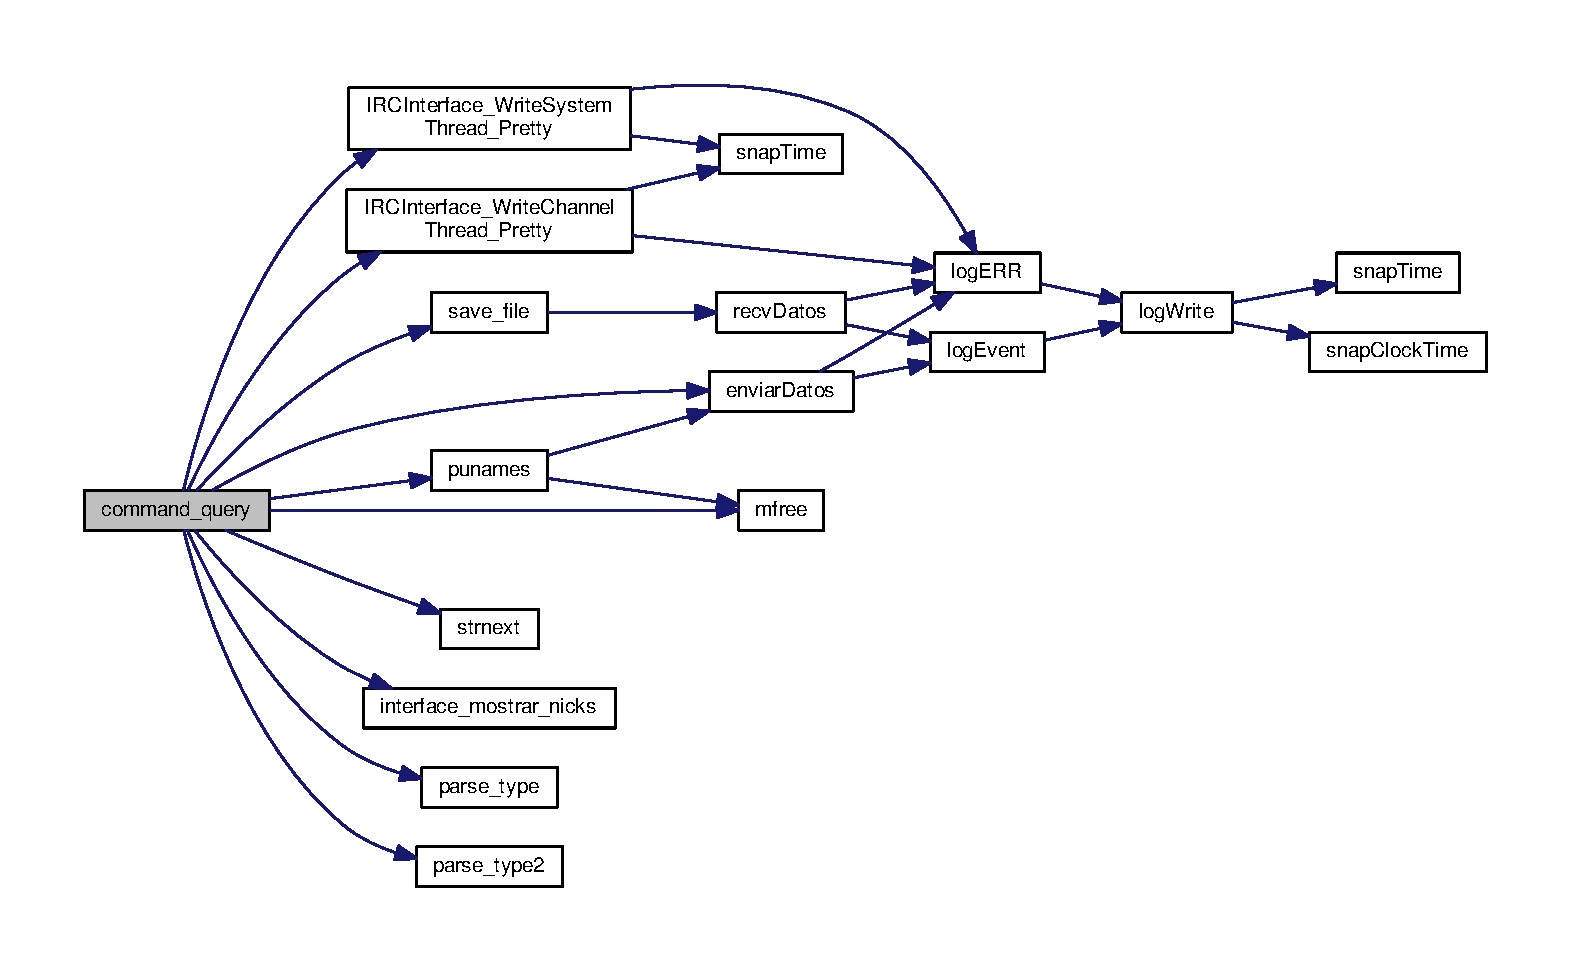
\includegraphics[width=350pt]{xchat2_8c_a41f93f364aea303a0c93177289733f92_cgraph}
\end{center}
\end{figure}


\hypertarget{xchat2_8c_a98484e1bbb136d37503aa6c604eff6a2}{\index{xchat2.\-c@{xchat2.\-c}!glue\-And\-Query@{glue\-And\-Query}}
\index{glue\-And\-Query@{glue\-And\-Query}!xchat2.c@{xchat2.\-c}}
\subsubsection[{glue\-And\-Query}]{\setlength{\rightskip}{0pt plus 5cm}void glue\-And\-Query (
\begin{DoxyParamCaption}
\item[{char $\ast$}]{command, }
\item[{char $\ast$}]{last\-\_\-command}
\end{DoxyParamCaption}
)}}\label{xchat2_8c_a98484e1bbb136d37503aa6c604eff6a2}

\begin{DoxyCode}
1003                                                     \{
1004         \textcolor{keywordtype}{char}* glued\_command = (\textcolor{keywordtype}{char}*) malloc((2 + strlen(command) + strlen(
      \hyperlink{xchat2_8c_a4e304440b657a8d3265793203cb12393}{last\_command})) * \textcolor{keyword}{sizeof}(char));
1005         
1006         strcpy(glued\_command, \hyperlink{xchat2_8c_a4e304440b657a8d3265793203cb12393}{last\_command});
1007         strcat(glued\_command, command);
1008 
1009         g\_print(\hyperlink{types_8h_add9307de87f38e77d336751e305886f6}{BLU} \textcolor{stringliteral}{"\(\backslash\)nglued\_command = %s\(\backslash\)n"} \hyperlink{types_8h_ab702106cf3b3e96750b6845ded4e0299}{RESET}, glued\_command);
1010         \hyperlink{xchat2_8c_a41f93f364aea303a0c93177289733f92}{command\_query}(glued\_command);
1011 
1012         free(command);
1013         free(glued\_command);
1014 \}
\end{DoxyCode}


Here is the call graph for this function\-:
\nopagebreak
\begin{figure}[H]
\begin{center}
\leavevmode
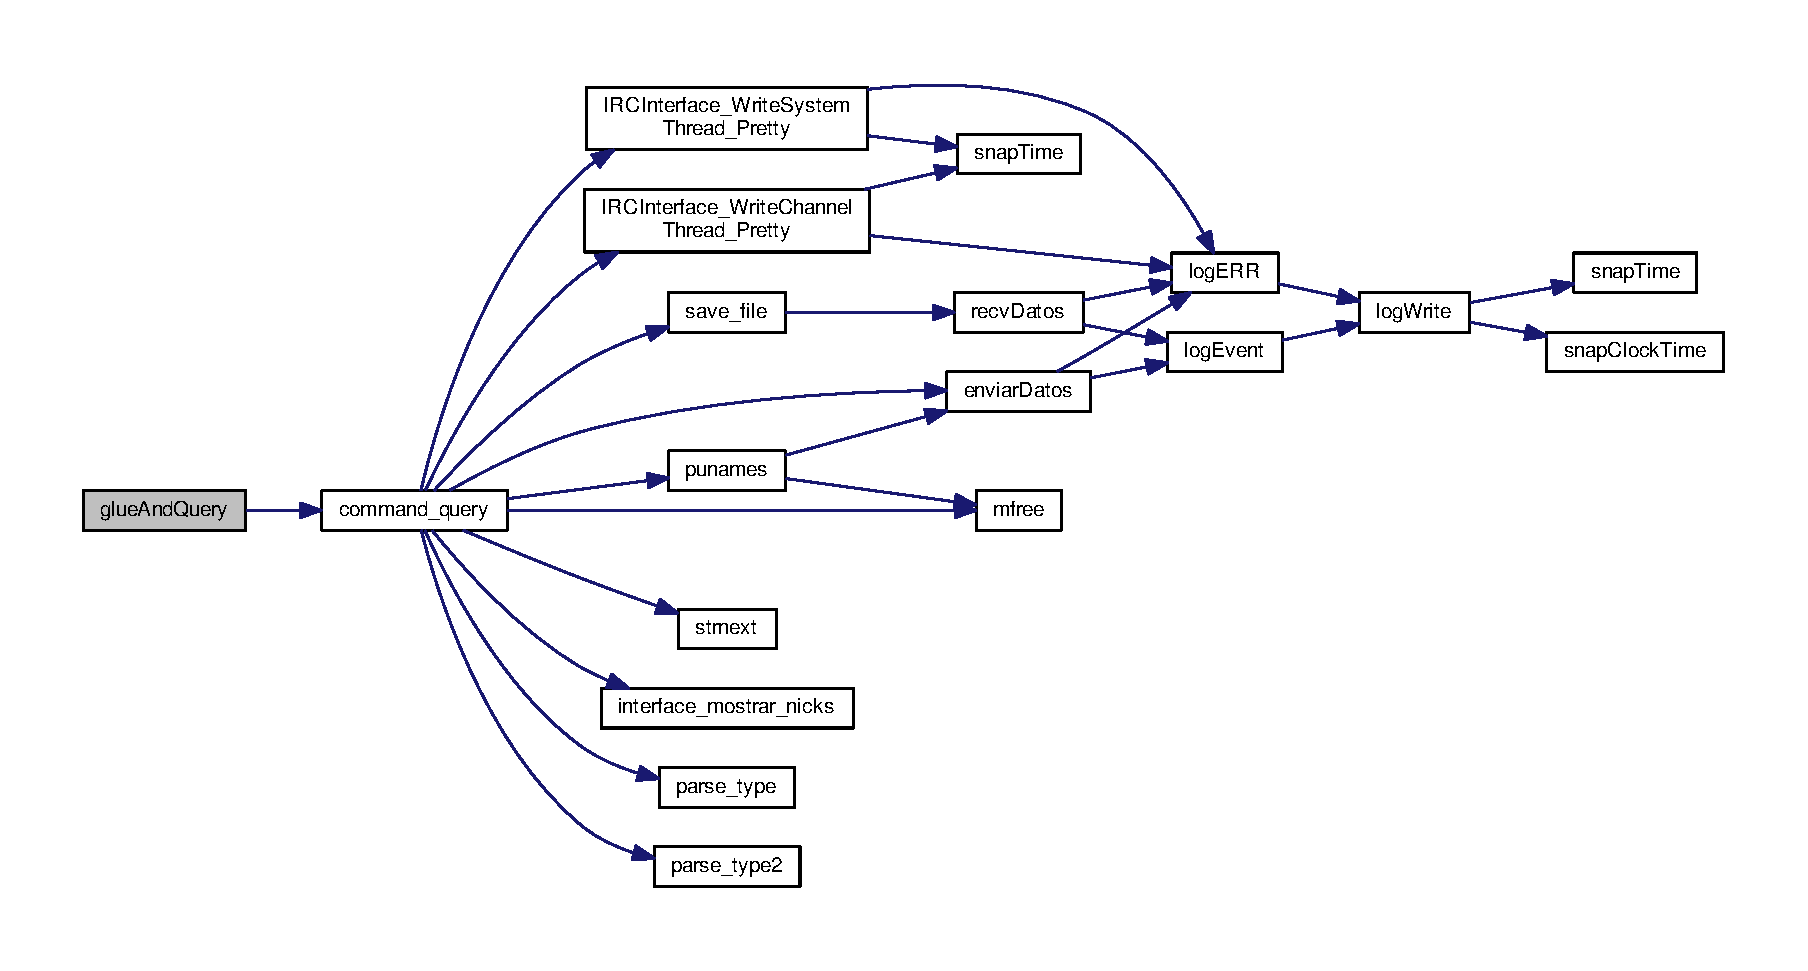
\includegraphics[width=350pt]{xchat2_8c_a98484e1bbb136d37503aa6c604eff6a2_cgraph}
\end{center}
\end{figure}


\hypertarget{xchat2_8c_a33f80a29a744e4182b29e23f13c1f05c}{\index{xchat2.\-c@{xchat2.\-c}!I\-R\-C\-Interface\-\_\-\-Activate\-Channel\-Key@{I\-R\-C\-Interface\-\_\-\-Activate\-Channel\-Key}}
\index{I\-R\-C\-Interface\-\_\-\-Activate\-Channel\-Key@{I\-R\-C\-Interface\-\_\-\-Activate\-Channel\-Key}!xchat2.c@{xchat2.\-c}}
\subsubsection[{I\-R\-C\-Interface\-\_\-\-Activate\-Channel\-Key}]{\setlength{\rightskip}{0pt plus 5cm}void I\-R\-C\-Interface\-\_\-\-Activate\-Channel\-Key (
\begin{DoxyParamCaption}
\item[{char $\ast$}]{channel, }
\item[{char $\ast$}]{key}
\end{DoxyParamCaption}
)}}\label{xchat2_8c_a33f80a29a744e4182b29e23f13c1f05c}

\begin{DoxyCode}
1222 \{
1223         \textcolor{keywordtype}{char} modo[\hyperlink{types_8h_ae7e715c270481406658bbd2bafa2897f}{MAXDATA}] = \{0\};
1224 
1225         g\_print(\hyperlink{types_8h_add9307de87f38e77d336751e305886f6}{BLU} \textcolor{stringliteral}{"\(\backslash\)nIRCInterface\_ActivateChannelKey(char *channel, char *key) call\(\backslash\)n"} 
      \hyperlink{types_8h_ab702106cf3b3e96750b6845ded4e0299}{RESET});
1226 
1227         sprintf(modo,\textcolor{stringliteral}{"+k %s"},key);
1228         \textcolor{keywordflow}{if} (\hyperlink{aux__functions_8h_a06340d30a60b297a60b17841767fad85}{changeMode}(channel, NULL, modo) != \hyperlink{daemon_8h_aba51915c87d64af47fb1cc59348961c9}{OK})
1229                 g\_print(\hyperlink{types_8h_a8d23feea868a983c8c2b661e1e16972f}{RED} \textcolor{stringliteral}{"ERROR - In IRCInterface\_ActivateChannelKey: Error en changeMode, devolvió
       ERR\(\backslash\)n"} \hyperlink{types_8h_ab702106cf3b3e96750b6845ded4e0299}{RESET});
1230 \}
\end{DoxyCode}


Here is the call graph for this function\-:
\nopagebreak
\begin{figure}[H]
\begin{center}
\leavevmode
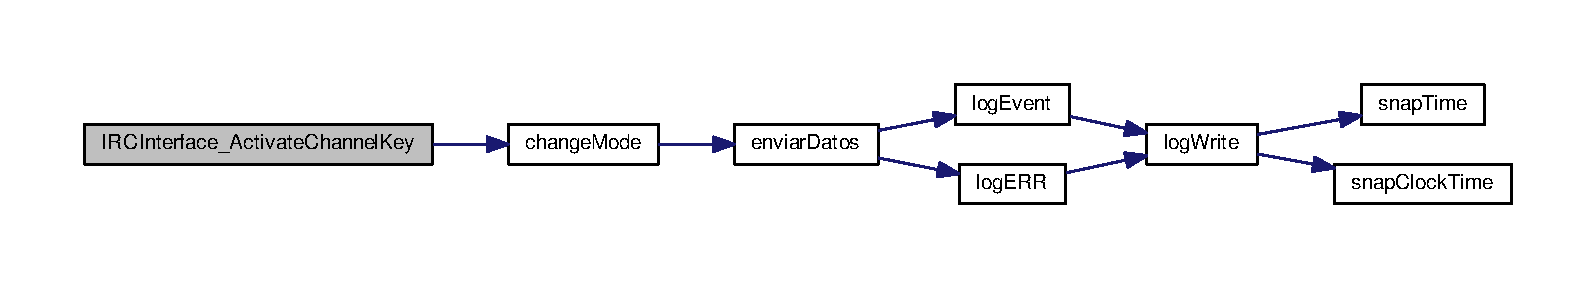
\includegraphics[width=350pt]{xchat2_8c_a33f80a29a744e4182b29e23f13c1f05c_cgraph}
\end{center}
\end{figure}


\hypertarget{xchat2_8c_a7a439929c246e342ae525139b2c39f5d}{\index{xchat2.\-c@{xchat2.\-c}!I\-R\-C\-Interface\-\_\-\-Activate\-External\-Messages@{I\-R\-C\-Interface\-\_\-\-Activate\-External\-Messages}}
\index{I\-R\-C\-Interface\-\_\-\-Activate\-External\-Messages@{I\-R\-C\-Interface\-\_\-\-Activate\-External\-Messages}!xchat2.c@{xchat2.\-c}}
\subsubsection[{I\-R\-C\-Interface\-\_\-\-Activate\-External\-Messages}]{\setlength{\rightskip}{0pt plus 5cm}void I\-R\-C\-Interface\-\_\-\-Activate\-External\-Messages (
\begin{DoxyParamCaption}
\item[{char $\ast$}]{channel}
\end{DoxyParamCaption}
)}}\label{xchat2_8c_a7a439929c246e342ae525139b2c39f5d}

\begin{DoxyCode}
1263 \{
1264         g\_print(\hyperlink{types_8h_add9307de87f38e77d336751e305886f6}{BLU} \textcolor{stringliteral}{"\(\backslash\)nIRCInterface\_ActivateExternalMessages(char *channel) call\(\backslash\)n"} 
      \hyperlink{types_8h_ab702106cf3b3e96750b6845ded4e0299}{RESET});
1265         \textcolor{keywordflow}{if} (\hyperlink{aux__functions_8h_a06340d30a60b297a60b17841767fad85}{changeMode}(channel, NULL, \textcolor{stringliteral}{"+n"}) != \hyperlink{daemon_8h_aba51915c87d64af47fb1cc59348961c9}{OK})
1266                 g\_print(\hyperlink{types_8h_a8d23feea868a983c8c2b661e1e16972f}{RED} \textcolor{stringliteral}{"ERROR - In IRCInterface\_ActivateExternalMessages: Error en changeMode,
       devolvió ERR\(\backslash\)n"} \hyperlink{types_8h_ab702106cf3b3e96750b6845ded4e0299}{RESET});
1267 \}
\end{DoxyCode}


Here is the call graph for this function\-:
\nopagebreak
\begin{figure}[H]
\begin{center}
\leavevmode
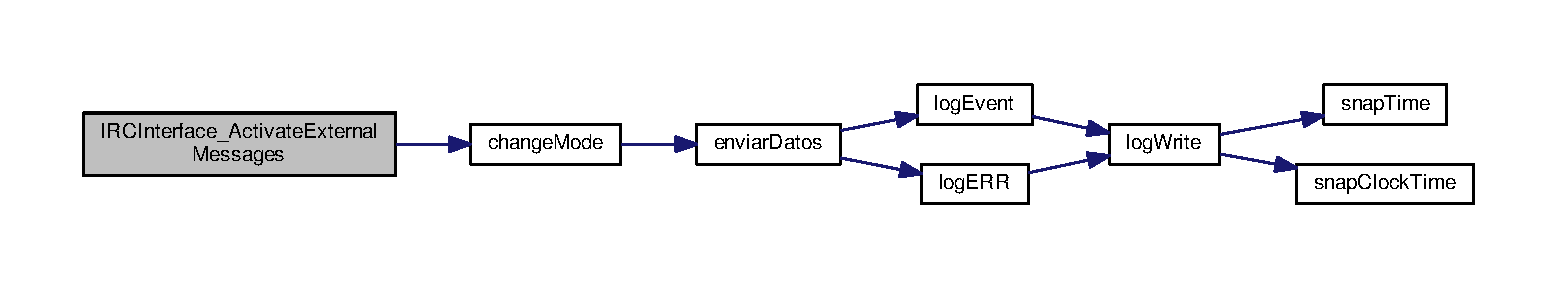
\includegraphics[width=350pt]{xchat2_8c_a7a439929c246e342ae525139b2c39f5d_cgraph}
\end{center}
\end{figure}


\hypertarget{xchat2_8c_ac72762ab1e3575b421b967241db23f9c}{\index{xchat2.\-c@{xchat2.\-c}!I\-R\-C\-Interface\-\_\-\-Activate\-Invite@{I\-R\-C\-Interface\-\_\-\-Activate\-Invite}}
\index{I\-R\-C\-Interface\-\_\-\-Activate\-Invite@{I\-R\-C\-Interface\-\_\-\-Activate\-Invite}!xchat2.c@{xchat2.\-c}}
\subsubsection[{I\-R\-C\-Interface\-\_\-\-Activate\-Invite}]{\setlength{\rightskip}{0pt plus 5cm}void I\-R\-C\-Interface\-\_\-\-Activate\-Invite (
\begin{DoxyParamCaption}
\item[{char $\ast$}]{channel}
\end{DoxyParamCaption}
)}}\label{xchat2_8c_ac72762ab1e3575b421b967241db23f9c}

\begin{DoxyCode}
1300 \{
1301         g\_print(\hyperlink{types_8h_add9307de87f38e77d336751e305886f6}{BLU} \textcolor{stringliteral}{"\(\backslash\)nIRCInterface\_ActivateInvite(char *channel) call\(\backslash\)n"} 
      \hyperlink{types_8h_ab702106cf3b3e96750b6845ded4e0299}{RESET});
1302         \textcolor{keywordflow}{if} (\hyperlink{aux__functions_8h_a06340d30a60b297a60b17841767fad85}{changeMode}(channel, NULL, \textcolor{stringliteral}{"+i"}) != \hyperlink{daemon_8h_aba51915c87d64af47fb1cc59348961c9}{OK})
1303                 g\_print(\hyperlink{types_8h_a8d23feea868a983c8c2b661e1e16972f}{RED} \textcolor{stringliteral}{"ERROR - In IRCInterface\_ActivateInvite: Error en changeMode, devolvió ERR\(\backslash\)n
      "} \hyperlink{types_8h_ab702106cf3b3e96750b6845ded4e0299}{RESET});
1304 \}
\end{DoxyCode}


Here is the call graph for this function\-:
\nopagebreak
\begin{figure}[H]
\begin{center}
\leavevmode
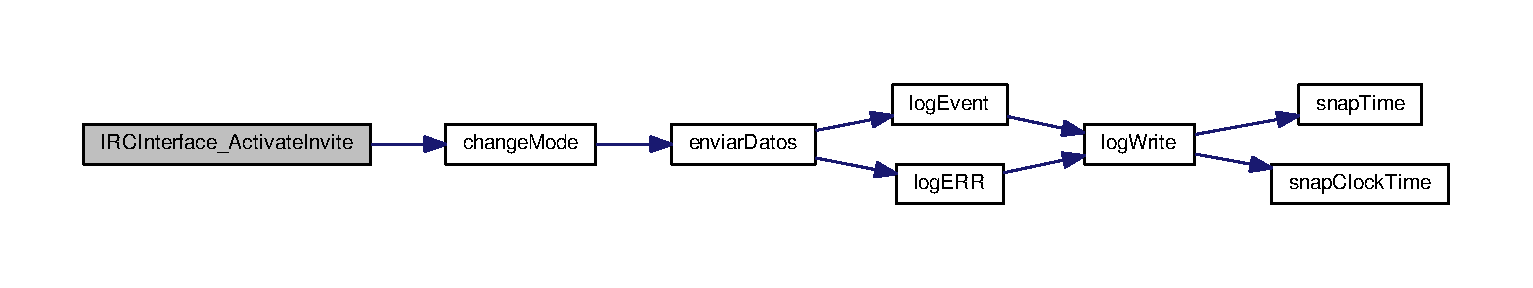
\includegraphics[width=350pt]{xchat2_8c_ac72762ab1e3575b421b967241db23f9c_cgraph}
\end{center}
\end{figure}


\hypertarget{xchat2_8c_af83498f4058311f4562c43a9b70566b2}{\index{xchat2.\-c@{xchat2.\-c}!I\-R\-C\-Interface\-\_\-\-Activate\-Moderated@{I\-R\-C\-Interface\-\_\-\-Activate\-Moderated}}
\index{I\-R\-C\-Interface\-\_\-\-Activate\-Moderated@{I\-R\-C\-Interface\-\_\-\-Activate\-Moderated}!xchat2.c@{xchat2.\-c}}
\subsubsection[{I\-R\-C\-Interface\-\_\-\-Activate\-Moderated}]{\setlength{\rightskip}{0pt plus 5cm}void I\-R\-C\-Interface\-\_\-\-Activate\-Moderated (
\begin{DoxyParamCaption}
\item[{char $\ast$}]{channel}
\end{DoxyParamCaption}
)}}\label{xchat2_8c_af83498f4058311f4562c43a9b70566b2}

\begin{DoxyCode}
1337 \{
1338         g\_print(\hyperlink{types_8h_add9307de87f38e77d336751e305886f6}{BLU} \textcolor{stringliteral}{"\(\backslash\)nIRCInterface\_ActivateModerated(char *channel) call\(\backslash\)n"} 
      \hyperlink{types_8h_ab702106cf3b3e96750b6845ded4e0299}{RESET});
1339 
1340         \textcolor{keywordflow}{if} (\hyperlink{aux__functions_8h_a06340d30a60b297a60b17841767fad85}{changeMode}(channel, NULL, \textcolor{stringliteral}{"+m"}) != \hyperlink{daemon_8h_aba51915c87d64af47fb1cc59348961c9}{OK})
1341                 g\_print(\hyperlink{types_8h_a8d23feea868a983c8c2b661e1e16972f}{RED} \textcolor{stringliteral}{"ERROR - In IRCInterface\_ActivateModerated: Error en changeMode, devolvió
       ERR\(\backslash\)n"} \hyperlink{types_8h_ab702106cf3b3e96750b6845ded4e0299}{RESET});
1342 \}
\end{DoxyCode}


Here is the call graph for this function\-:
\nopagebreak
\begin{figure}[H]
\begin{center}
\leavevmode
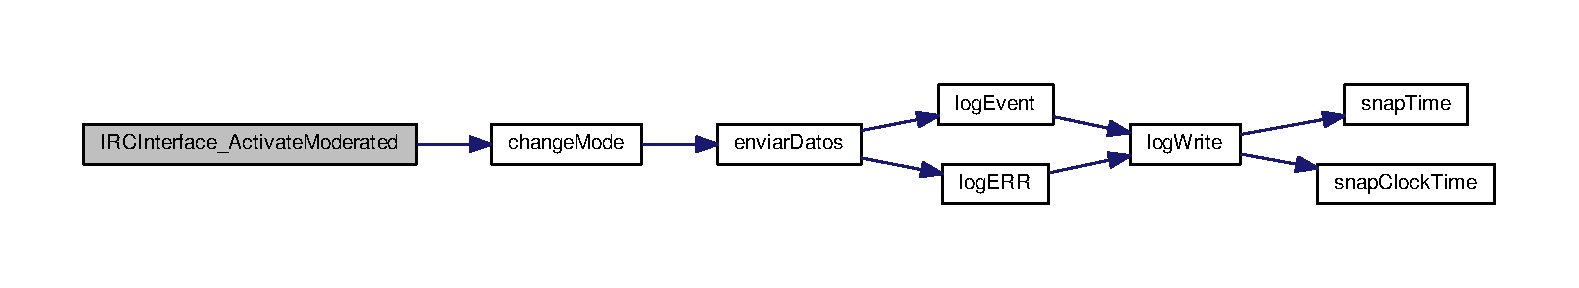
\includegraphics[width=350pt]{xchat2_8c_af83498f4058311f4562c43a9b70566b2_cgraph}
\end{center}
\end{figure}


\hypertarget{xchat2_8c_ab5694cc413472173bfcaa969c7d9800e}{\index{xchat2.\-c@{xchat2.\-c}!I\-R\-C\-Interface\-\_\-\-Activate\-Nicks\-Limit@{I\-R\-C\-Interface\-\_\-\-Activate\-Nicks\-Limit}}
\index{I\-R\-C\-Interface\-\_\-\-Activate\-Nicks\-Limit@{I\-R\-C\-Interface\-\_\-\-Activate\-Nicks\-Limit}!xchat2.c@{xchat2.\-c}}
\subsubsection[{I\-R\-C\-Interface\-\_\-\-Activate\-Nicks\-Limit}]{\setlength{\rightskip}{0pt plus 5cm}void I\-R\-C\-Interface\-\_\-\-Activate\-Nicks\-Limit (
\begin{DoxyParamCaption}
\item[{char $\ast$}]{channel, }
\item[{int}]{limit}
\end{DoxyParamCaption}
)}}\label{xchat2_8c_ab5694cc413472173bfcaa969c7d9800e}

\begin{DoxyCode}
1378 \{
1379         \textcolor{keywordtype}{char} mode[\hyperlink{types_8h_ae7e715c270481406658bbd2bafa2897f}{MAXDATA}] = \{0\};
1380 
1381         g\_print(\hyperlink{types_8h_add9307de87f38e77d336751e305886f6}{BLU} \textcolor{stringliteral}{"\(\backslash\)nIRCInterface\_ActivateNicksLimit(char *channel, int limit) call\(\backslash\)n"} 
      \hyperlink{types_8h_ab702106cf3b3e96750b6845ded4e0299}{RESET});
1382 
1383         sprintf(mode,\textcolor{stringliteral}{"+l %d"},limit);
1384         \textcolor{keywordflow}{if} (\hyperlink{aux__functions_8h_a06340d30a60b297a60b17841767fad85}{changeMode}(channel, NULL, mode) != \hyperlink{daemon_8h_aba51915c87d64af47fb1cc59348961c9}{OK})
1385                 g\_print(\hyperlink{types_8h_a8d23feea868a983c8c2b661e1e16972f}{RED} \textcolor{stringliteral}{"ERROR - In IRCInterface\_ActivateNicksLimit: Error en changeMode, devolvió
       ERR\(\backslash\)n"} \hyperlink{types_8h_ab702106cf3b3e96750b6845ded4e0299}{RESET});
1386 \}
\end{DoxyCode}


Here is the call graph for this function\-:
\nopagebreak
\begin{figure}[H]
\begin{center}
\leavevmode
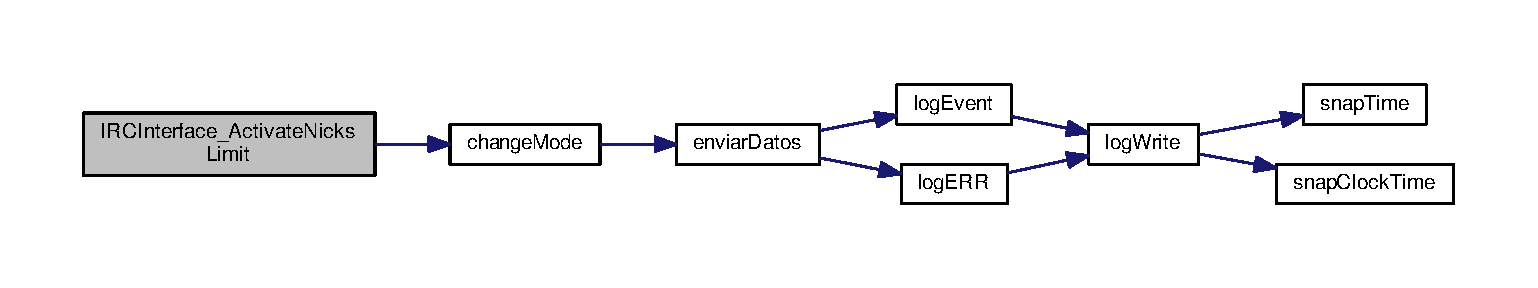
\includegraphics[width=350pt]{xchat2_8c_ab5694cc413472173bfcaa969c7d9800e_cgraph}
\end{center}
\end{figure}


\hypertarget{xchat2_8c_ab1f09c737c7c109a97e22de6072d731d}{\index{xchat2.\-c@{xchat2.\-c}!I\-R\-C\-Interface\-\_\-\-Activate\-Private@{I\-R\-C\-Interface\-\_\-\-Activate\-Private}}
\index{I\-R\-C\-Interface\-\_\-\-Activate\-Private@{I\-R\-C\-Interface\-\_\-\-Activate\-Private}!xchat2.c@{xchat2.\-c}}
\subsubsection[{I\-R\-C\-Interface\-\_\-\-Activate\-Private}]{\setlength{\rightskip}{0pt plus 5cm}void I\-R\-C\-Interface\-\_\-\-Activate\-Private (
\begin{DoxyParamCaption}
\item[{char $\ast$}]{channel}
\end{DoxyParamCaption}
)}}\label{xchat2_8c_ab1f09c737c7c109a97e22de6072d731d}

\begin{DoxyCode}
1419 \{
1420         g\_print(\hyperlink{types_8h_add9307de87f38e77d336751e305886f6}{BLU} \textcolor{stringliteral}{"\(\backslash\)nIRCInterface\_ActivatePrivate(char *channel) call\(\backslash\)n"} 
      \hyperlink{types_8h_ab702106cf3b3e96750b6845ded4e0299}{RESET});
1421         \textcolor{keywordflow}{if} (\hyperlink{aux__functions_8h_a06340d30a60b297a60b17841767fad85}{changeMode}(channel, NULL, \textcolor{stringliteral}{"+p"}) != \hyperlink{daemon_8h_aba51915c87d64af47fb1cc59348961c9}{OK})
1422                 g\_print(\hyperlink{types_8h_a8d23feea868a983c8c2b661e1e16972f}{RED} \textcolor{stringliteral}{"ERROR - In IRCInterface\_ActivatePrivate: Error en changeMode, devolvió ERR
      \(\backslash\)n"} \hyperlink{types_8h_ab702106cf3b3e96750b6845ded4e0299}{RESET});
1423 \}
\end{DoxyCode}


Here is the call graph for this function\-:
\nopagebreak
\begin{figure}[H]
\begin{center}
\leavevmode
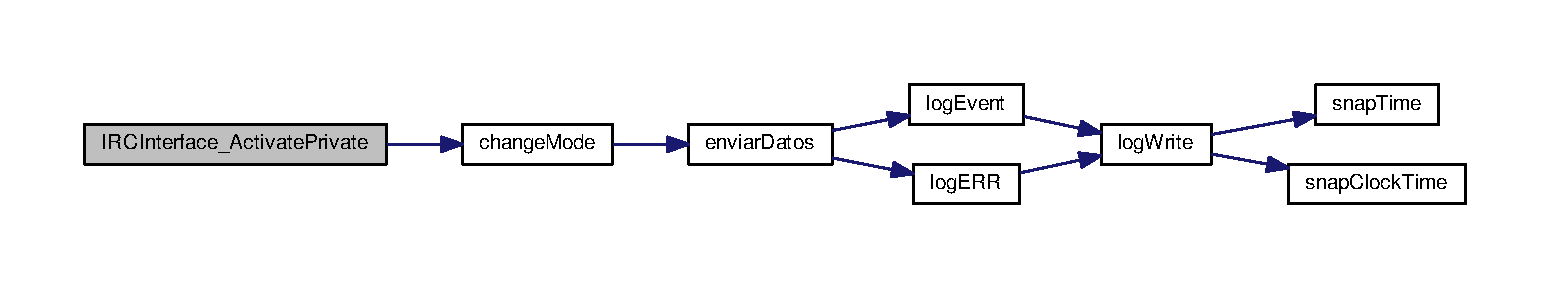
\includegraphics[width=350pt]{xchat2_8c_ab1f09c737c7c109a97e22de6072d731d_cgraph}
\end{center}
\end{figure}


\hypertarget{xchat2_8c_ac45f12d4dcacf3b5485eec6fdc51df93}{\index{xchat2.\-c@{xchat2.\-c}!I\-R\-C\-Interface\-\_\-\-Activate\-Protect\-Topic@{I\-R\-C\-Interface\-\_\-\-Activate\-Protect\-Topic}}
\index{I\-R\-C\-Interface\-\_\-\-Activate\-Protect\-Topic@{I\-R\-C\-Interface\-\_\-\-Activate\-Protect\-Topic}!xchat2.c@{xchat2.\-c}}
\subsubsection[{I\-R\-C\-Interface\-\_\-\-Activate\-Protect\-Topic}]{\setlength{\rightskip}{0pt plus 5cm}void I\-R\-C\-Interface\-\_\-\-Activate\-Protect\-Topic (
\begin{DoxyParamCaption}
\item[{char $\ast$}]{channel}
\end{DoxyParamCaption}
)}}\label{xchat2_8c_ac45f12d4dcacf3b5485eec6fdc51df93}

\begin{DoxyCode}
1456 \{
1457         g\_print(\hyperlink{types_8h_add9307de87f38e77d336751e305886f6}{BLU} \textcolor{stringliteral}{"\(\backslash\)nIRCInterface\_ActivateProtectTopic(char *channel) call\(\backslash\)n"} 
      \hyperlink{types_8h_ab702106cf3b3e96750b6845ded4e0299}{RESET});
1458         \textcolor{keywordflow}{if} (\hyperlink{aux__functions_8h_a06340d30a60b297a60b17841767fad85}{changeMode}(channel, NULL, \textcolor{stringliteral}{"+t"}) != \hyperlink{daemon_8h_aba51915c87d64af47fb1cc59348961c9}{OK})
1459                 g\_print(\hyperlink{types_8h_a8d23feea868a983c8c2b661e1e16972f}{RED} \textcolor{stringliteral}{"ERROR - In IRCInterface\_ActivateProtectTopic: Error en changeMode, devolvió
       ERR\(\backslash\)n"} \hyperlink{types_8h_ab702106cf3b3e96750b6845ded4e0299}{RESET});
1460 \}
\end{DoxyCode}


Here is the call graph for this function\-:
\nopagebreak
\begin{figure}[H]
\begin{center}
\leavevmode
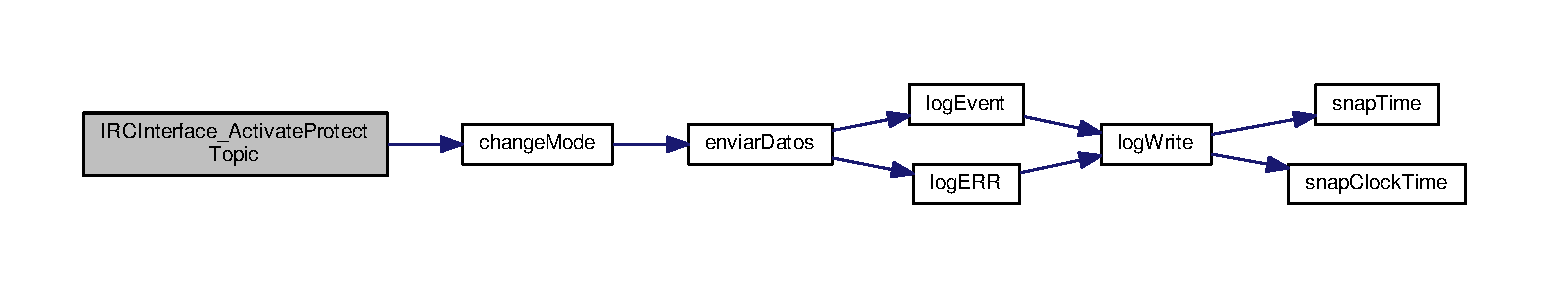
\includegraphics[width=350pt]{xchat2_8c_ac45f12d4dcacf3b5485eec6fdc51df93_cgraph}
\end{center}
\end{figure}


\hypertarget{xchat2_8c_aa9e9155115b834d85a4d10cb27f99093}{\index{xchat2.\-c@{xchat2.\-c}!I\-R\-C\-Interface\-\_\-\-Activate\-Secret@{I\-R\-C\-Interface\-\_\-\-Activate\-Secret}}
\index{I\-R\-C\-Interface\-\_\-\-Activate\-Secret@{I\-R\-C\-Interface\-\_\-\-Activate\-Secret}!xchat2.c@{xchat2.\-c}}
\subsubsection[{I\-R\-C\-Interface\-\_\-\-Activate\-Secret}]{\setlength{\rightskip}{0pt plus 5cm}void I\-R\-C\-Interface\-\_\-\-Activate\-Secret (
\begin{DoxyParamCaption}
\item[{char $\ast$}]{channel}
\end{DoxyParamCaption}
)}}\label{xchat2_8c_aa9e9155115b834d85a4d10cb27f99093}

\begin{DoxyCode}
1493 \{
1494         g\_print(\hyperlink{types_8h_add9307de87f38e77d336751e305886f6}{BLU} \textcolor{stringliteral}{"\(\backslash\)nIRCInterface\_ActivateSecret(char *channel) call\(\backslash\)n"} 
      \hyperlink{types_8h_ab702106cf3b3e96750b6845ded4e0299}{RESET});
1495 
1496         \textcolor{keywordflow}{if} (\hyperlink{aux__functions_8h_a06340d30a60b297a60b17841767fad85}{changeMode}(channel, NULL, \textcolor{stringliteral}{"+s"}) != \hyperlink{daemon_8h_aba51915c87d64af47fb1cc59348961c9}{OK})
1497                 g\_print(\hyperlink{types_8h_a8d23feea868a983c8c2b661e1e16972f}{RED} \textcolor{stringliteral}{"ERROR - In IRCInterface\_ActivateSecret: Error en changeMode, devolvió ERR\(\backslash\)n
      "} \hyperlink{types_8h_ab702106cf3b3e96750b6845ded4e0299}{RESET});
1498 \}
\end{DoxyCode}


Here is the call graph for this function\-:
\nopagebreak
\begin{figure}[H]
\begin{center}
\leavevmode
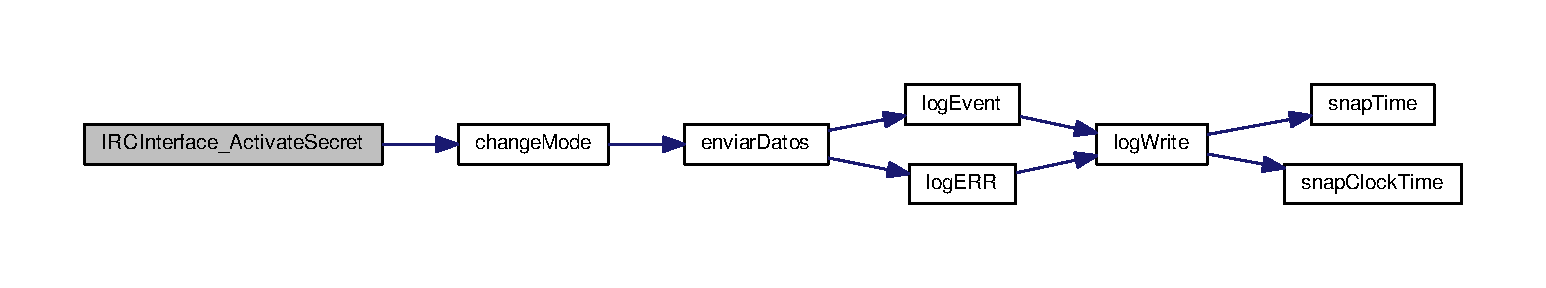
\includegraphics[width=350pt]{xchat2_8c_aa9e9155115b834d85a4d10cb27f99093_cgraph}
\end{center}
\end{figure}


\hypertarget{xchat2_8c_a42773b5a840f9d0455f148d285e1e595}{\index{xchat2.\-c@{xchat2.\-c}!I\-R\-C\-Interface\-\_\-\-Ban\-Nick@{I\-R\-C\-Interface\-\_\-\-Ban\-Nick}}
\index{I\-R\-C\-Interface\-\_\-\-Ban\-Nick@{I\-R\-C\-Interface\-\_\-\-Ban\-Nick}!xchat2.c@{xchat2.\-c}}
\subsubsection[{I\-R\-C\-Interface\-\_\-\-Ban\-Nick}]{\setlength{\rightskip}{0pt plus 5cm}void I\-R\-C\-Interface\-\_\-\-Ban\-Nick (
\begin{DoxyParamCaption}
\item[{char $\ast$}]{channel, }
\item[{char $\ast$}]{nick}
\end{DoxyParamCaption}
)}}\label{xchat2_8c_a42773b5a840f9d0455f148d285e1e595}

\begin{DoxyCode}
1533 \{
1534         g\_print(\hyperlink{types_8h_add9307de87f38e77d336751e305886f6}{BLU} \textcolor{stringliteral}{"\(\backslash\)nIRCInterface\_BanNick(char *channel, char *nick) call\(\backslash\)n"} 
      \hyperlink{types_8h_ab702106cf3b3e96750b6845ded4e0299}{RESET});
1535 
1536         \textcolor{keywordflow}{if} (\hyperlink{aux__functions_8h_a06340d30a60b297a60b17841767fad85}{changeMode}(channel, nick, \textcolor{stringliteral}{"+b"}) != \hyperlink{daemon_8h_aba51915c87d64af47fb1cc59348961c9}{OK})
1537                 g\_print(\hyperlink{types_8h_a8d23feea868a983c8c2b661e1e16972f}{RED} \textcolor{stringliteral}{"ERROR - In IRCInterface\_BanNick: Error en changeMode, devolvió ERR\(\backslash\)n"} 
      \hyperlink{types_8h_ab702106cf3b3e96750b6845ded4e0299}{RESET});
1538 \}
\end{DoxyCode}


Here is the call graph for this function\-:
\nopagebreak
\begin{figure}[H]
\begin{center}
\leavevmode
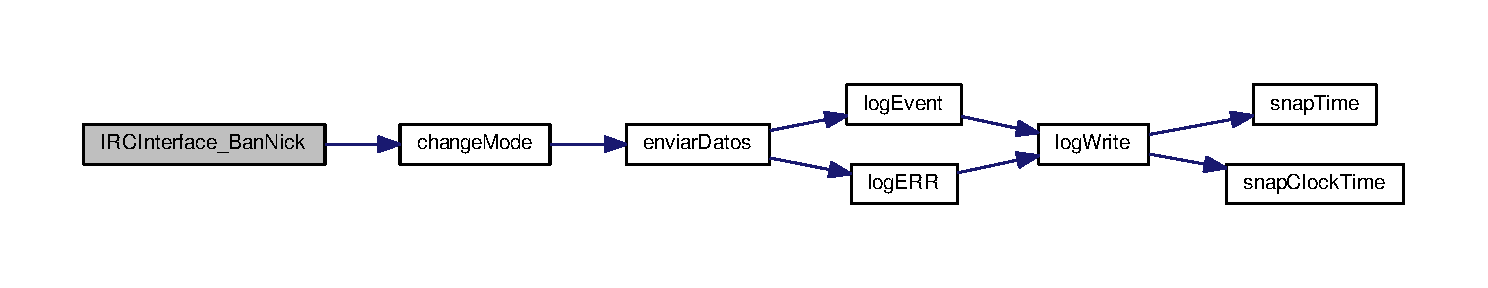
\includegraphics[width=350pt]{xchat2_8c_a42773b5a840f9d0455f148d285e1e595_cgraph}
\end{center}
\end{figure}


\hypertarget{xchat2_8c_aed072f4ce0d6e90697d4d6eb0278a2ad}{\index{xchat2.\-c@{xchat2.\-c}!I\-R\-C\-Interface\-\_\-\-Connect@{I\-R\-C\-Interface\-\_\-\-Connect}}
\index{I\-R\-C\-Interface\-\_\-\-Connect@{I\-R\-C\-Interface\-\_\-\-Connect}!xchat2.c@{xchat2.\-c}}
\subsubsection[{I\-R\-C\-Interface\-\_\-\-Connect}]{\setlength{\rightskip}{0pt plus 5cm}long I\-R\-C\-Interface\-\_\-\-Connect (
\begin{DoxyParamCaption}
\item[{char $\ast$}]{nick, }
\item[{char $\ast$}]{user, }
\item[{char $\ast$}]{realname, }
\item[{char $\ast$}]{password, }
\item[{char $\ast$}]{server, }
\item[{int}]{port, }
\item[{boolean}]{ssl}
\end{DoxyParamCaption}
)}}\label{xchat2_8c_aed072f4ce0d6e90697d4d6eb0278a2ad}

\begin{DoxyCode}
1585 \{
1586         \textcolor{keywordtype}{int} optval = 1;
1587         \textcolor{keywordtype}{long} ret = -1;
1588         \textcolor{keywordtype}{int} retorno = -1;
1589         \textcolor{keywordtype}{char} *command = NULL;
1590         \textcolor{keywordtype}{char} *prefix = NULL;
1591         \textcolor{keywordtype}{int} sockfd = -1;
1592 
1593         \textcolor{keyword}{struct }hostent *he;
1594     \textcolor{keyword}{struct }in\_addr **addr\_list;
1595     \textcolor{keywordtype}{int} i=0;
1596     \textcolor{keywordtype}{char} ip\_addr[INET\_ADDRSTRLEN] = \{0\};
1597 
1598     \textcolor{keywordtype}{char} *msgNick = NULL;
1599     \textcolor{keywordtype}{char} mode[\hyperlink{types_8h_ae7e715c270481406658bbd2bafa2897f}{MAXDATA}] = \{0\};
1600 
1601         g\_print(\textcolor{stringliteral}{"IRCInterface\_Connect - Datos introducidos por el usuario \(\backslash\)n"});
1602         g\_print(\textcolor{stringliteral}{"\(\backslash\)t nick: %s \(\backslash\)n"},nick);
1603         g\_print(\textcolor{stringliteral}{"\(\backslash\)t user: %s \(\backslash\)n"},user);
1604         g\_print(\textcolor{stringliteral}{"\(\backslash\)t realname: %s \(\backslash\)n"},realname);
1605         g\_print(\textcolor{stringliteral}{"\(\backslash\)t password: %s \(\backslash\)n"},password);
1606         g\_print(\textcolor{stringliteral}{"\(\backslash\)t server: %s \(\backslash\)n"},server);
1607         g\_print(\textcolor{stringliteral}{"\(\backslash\)t port: %d \(\backslash\)n"},port);
1608         g\_print(\textcolor{stringliteral}{"\(\backslash\)t ssl: %d \(\backslash\)n"},ssl);
1609 
1610     \textcolor{keywordflow}{if} ((he = gethostbyname(server)) == NULL) \{  \textcolor{comment}{// get the host info}
1611         g\_print(\hyperlink{types_8h_a8d23feea868a983c8c2b661e1e16972f}{RED} \textcolor{stringliteral}{"ERROR - In IRCInterface\_Connect: gethostbyname() devol NULL\(\backslash\)n"} 
      \hyperlink{types_8h_ab702106cf3b3e96750b6845ded4e0299}{RESET});
1612         \textcolor{keywordflow}{return} IRCERR\_NOCONNECT;
1613     \}
1614 
1615     \textcolor{comment}{// print information about this host:}
1616     g\_print(\textcolor{stringliteral}{"Official name is: %s\(\backslash\)n"}, he->h\_name);
1617     g\_print(\textcolor{stringliteral}{"    IP addresses: "});
1618 
1619     addr\_list = (\textcolor{keyword}{struct }in\_addr **)he->h\_addr\_list;
1620     \textcolor{keywordflow}{for}(i = 0; addr\_list[i] != NULL; i++) \{
1621         strcat(ip\_addr,inet\_ntoa(*addr\_list[i]));
1622         g\_print(\textcolor{stringliteral}{"%s "}, inet\_ntoa(*addr\_list[i]));
1623     \}
1624     g\_print(\textcolor{stringliteral}{"\(\backslash\)n"});
1625     g\_print(\textcolor{stringliteral}{"ip\_addr: %s \(\backslash\)n"},ip\_addr);
1626 
1627     \textcolor{keyword}{struct }sockaddr\_in server\_struct;
1628 
1629     \textcolor{comment}{/*Socket*/}
1630     sockfd = socket(AF\_INET,SOCK\_STREAM,0\textcolor{comment}{/*TCP*/});
1631     \textcolor{keywordflow}{if} (sockfd == -1)\{
1632         g\_print(\hyperlink{types_8h_a8d23feea868a983c8c2b661e1e16972f}{RED} \textcolor{stringliteral}{"ERROR - In IRCInterface\_Connect: Error creando socket, devolvió < 0\(\backslash\)n"} 
      \hyperlink{types_8h_ab702106cf3b3e96750b6845ded4e0299}{RESET});
1633         \textcolor{keywordflow}{return} IRCERR\_NOCONNECT;
1634     \}
1635 
1636     optval = 1;
1637     setsockopt(sockfd, SOL\_SOCKET, SO\_REUSEADDR, (\textcolor{keyword}{const} \textcolor{keywordtype}{void} *)&optval , \textcolor{keyword}{sizeof}(\textcolor{keywordtype}{int})); \textcolor{comment}{//reutilizar socket
       sucesivas ejecuciones}
1638 
1639     memset(&server\_struct, \textcolor{charliteral}{'0'}, \textcolor{keyword}{sizeof}(server\_struct)); 
1640     server\_struct.sin\_family = AF\_INET;
1641     server\_struct.sin\_port = htons(port); 
1642     memset(&(server\_struct.sin\_zero), \textcolor{charliteral}{'\(\backslash\)0'}, 8);
1643     server\_struct.sin\_addr = **addr\_list; 
1644 
1645     \textcolor{comment}{/*Connect*/}
1646     \textcolor{keywordflow}{if} (connect(sockfd, (\textcolor{keyword}{struct} sockaddr*)&server\_struct, \textcolor{keyword}{sizeof}(server\_struct)) < 0)\{
1647         g\_print(\hyperlink{types_8h_a8d23feea868a983c8c2b661e1e16972f}{RED} \textcolor{stringliteral}{"ERROR - In IRCInterface\_Connect: Error en connect(), devolivó < 0\(\backslash\)n"} 
      \hyperlink{types_8h_ab702106cf3b3e96750b6845ded4e0299}{RESET});
1648         \textcolor{keywordflow}{return} IRCERR\_NOCONNECT;
1649     \}
1650 
1651         \textcolor{comment}{//Conectarse al socket}
1652         \textcolor{comment}{//sockfd = clienteConexionTCP(ip\_addr,port);}
1653         \textcolor{keywordflow}{if}(sockfd == -1)\{
1654                 g\_print(\hyperlink{types_8h_a8d23feea868a983c8c2b661e1e16972f}{RED} \textcolor{stringliteral}{"ERROR - In IRCInterface\_Connect: sockfd == -1\(\backslash\)n"} 
      \hyperlink{types_8h_ab702106cf3b3e96750b6845ded4e0299}{RESET});
1655                 \textcolor{keywordflow}{return} IRCERR\_NOCONNECT;
1656         \}\textcolor{keywordflow}{else}\{
1657                 g\_print(\hyperlink{types_8h_aea69ffbacdcdf16c21b8c9961df84448}{GRN} \textcolor{stringliteral}{"Conexión establecida con host: %s y puerto: %d \(\backslash\)n"} 
      \hyperlink{types_8h_ab702106cf3b3e96750b6845ded4e0299}{RESET}, server, port);
1658         \}
1659 
1660         \textcolor{comment}{//Copiar los parametros a las variables globales}
1661         strcpy(\hyperlink{xchat2_8c_a738cdcabc13fa13e8263986fe5d0fc28}{host\_name}, he->h\_name);
1662     strcpy(\hyperlink{xchat2_8c_a7e2f32e47f3780a66e19651d8e79bced}{nick\_user},nick);
1663     \hyperlink{xchat2_8c_acd63fb8dbd9439219e2db08dfc173aa0}{sockfd\_user} = sockfd;
1664 
1665         \textcolor{keywordflow}{if}(ssl == FALSE)\{
1666                 g\_print(\hyperlink{types_8h_aea69ffbacdcdf16c21b8c9961df84448}{GRN} \textcolor{stringliteral}{"Lanzamos el hilo que recibe mensajes\(\backslash\)n"} \hyperlink{types_8h_ab702106cf3b3e96750b6845ded4e0299}{RESET});
1667                 \textcolor{keywordflow}{if}((ret = pthread\_create( &\hyperlink{xchat2_8c_ab5efd1efa144e252f4c5312ae57bea2e}{recv\_tid}, NULL, (\textcolor{keywordtype}{void}*) 
      \hyperlink{xchat2_8c_a7230d43b8458797c679e7180bf1fda90}{receive\_messages}, (\textcolor{keywordtype}{void}*) \textcolor{stringliteral}{"no\_arg"})) != 0)\{
1668                 g\_print(\hyperlink{types_8h_a8d23feea868a983c8c2b661e1e16972f}{RED} \textcolor{stringliteral}{"ERROR - In IRCInterface\_Connect: pthread\_create() devolvio != 0, error = %d
      \(\backslash\)n"} \hyperlink{types_8h_ab702106cf3b3e96750b6845ded4e0299}{RESET}, (\textcolor{keywordtype}{int})ret);
1669                 \textcolor{comment}{//logERR("pthread\_detach() devolvio error");}
1670                         \textcolor{keywordflow}{return} \hyperlink{types_8h_a735563036dced0b7d6cc98f97ea4978b}{ERR};
1671                 \}
1672 
1673                 \textcolor{keywordflow}{if} (pthread\_detach(\hyperlink{xchat2_8c_ab5efd1efa144e252f4c5312ae57bea2e}{recv\_tid}) != \hyperlink{daemon_8h_aba51915c87d64af47fb1cc59348961c9}{OK})\{
1674                         g\_print(\hyperlink{types_8h_a8d23feea868a983c8c2b661e1e16972f}{RED} \textcolor{stringliteral}{"ERROR - In IRCInterface\_Connect: pthread\_detach() devolvio error\(\backslash\)n"}
       \hyperlink{types_8h_ab702106cf3b3e96750b6845ded4e0299}{RESET});
1675                          \textcolor{comment}{//logERR("pthread\_detach() devolvio error");}
1676                          \textcolor{keywordflow}{return} \hyperlink{types_8h_a735563036dced0b7d6cc98f97ea4978b}{ERR};
1677                 \}
1678                 \textcolor{comment}{//sleep(5);}
1679                 \textcolor{comment}{//Prueba CAP}
1680                 \textcolor{comment}{/*}
1681 \textcolor{comment}{                retorno = enviarDatos(sockfd, "CAP LS 302", strlen("CAP LS 302")+1);}
1682 \textcolor{comment}{                if(retorno <= 0)\{}
1683 \textcolor{comment}{                        g\_print(RED "ERROR - In IRCInterface\_Connect: enviarDatos() envió %d Bytes -
       NICK\(\backslash\)n" RESET, retorno);}
1684 \textcolor{comment}{                        return IRCERR\_NOCONNECT;}
1685 \textcolor{comment}{                \}}
1686 \textcolor{comment}{                IRCInterface\_PlaneRegisterOutMessage(command);}
1687 \textcolor{comment}{                */}
1688 
1689                 \textcolor{comment}{//Enviar pass si existe}
1690                 \textcolor{keywordflow}{if}((password != NULL) && (strlen(password) > 0))\{ \textcolor{comment}{//Comprobar si hay password}
1691                         \textcolor{comment}{//Enviar mensaje al servidor con la pass}
1692                         ret = IRCMsg\_Pass (&command, prefix, password);
1693                         \textcolor{keywordflow}{if}(ret != IRC\_OK)\{
1694                                 g\_print(\hyperlink{types_8h_a8d23feea868a983c8c2b661e1e16972f}{RED} \textcolor{stringliteral}{"ERROR - In IRCInterface\_Connect: IRCMsg\_Pass devolvio
       IRCERR\_NOPASSWORD: No se ha introducido una clave.\(\backslash\)n"} \hyperlink{types_8h_ab702106cf3b3e96750b6845ded4e0299}{RESET});
1695                                 \textcolor{keywordflow}{return} IRCERR\_NOCONNECT;
1696                         \}
1697                         g\_print(\textcolor{stringliteral}{"IRCMsg\_Pass: %s"},command);
1698                         retorno = \hyperlink{conexion__tcp_8h_ab9468ce1338cfca5736ab407ba155f55}{enviarDatos}(sockfd, command, strlen(command));
1699                         \textcolor{keywordflow}{if}(retorno <= 0)\{
1700                                 g\_print(\hyperlink{types_8h_a8d23feea868a983c8c2b661e1e16972f}{RED} \textcolor{stringliteral}{"ERROR - In IRCInterface\_Connect: enviarDatos() envió %d
       Bytes - PASS\(\backslash\)n"} \hyperlink{types_8h_ab702106cf3b3e96750b6845ded4e0299}{RESET}, retorno);
1701                                 \textcolor{keywordflow}{return} IRCERR\_NOCONNECT;
1702                         \}
1703                         IRCInterface\_PlaneRegisterOutMessage(command); \textcolor{comment}{//Mandar a registro plano}
1704                         free(command);          
1705 
1706                 \}
1707 
1708                 \textcolor{comment}{//Enviar mensaje con el nick}
1709                 command = NULL;
1710                 ret = IRCMsg\_Nick (&command, prefix, nick, msgNick);
1711                 
1712                 \textcolor{keywordflow}{if}(ret != IRC\_OK)\{
1713                         g\_print(\hyperlink{types_8h_a8d23feea868a983c8c2b661e1e16972f}{RED} \textcolor{stringliteral}{"ERROR - In IRCInterface\_Connect: IRCMsg\_Nick() devolvio codigo de
       error\(\backslash\)n"} \hyperlink{types_8h_ab702106cf3b3e96750b6845ded4e0299}{RESET});
1714                         \textcolor{keywordflow}{return} IRCERR\_NOCONNECT;
1715                 \}
1716                 g\_print(\textcolor{stringliteral}{"IRCMsg\_Nick: %s"},command);
1717 
1718                 retorno = \hyperlink{conexion__tcp_8h_ab9468ce1338cfca5736ab407ba155f55}{enviarDatos}(sockfd, command, strlen(command));
1719                 \textcolor{comment}{//retorno = enviarDatos(sockfd, "NICK test\_\(\backslash\)r\(\backslash\)n\(\backslash\)0", strlen("NICK test\_\(\backslash\)r\(\backslash\)n\(\backslash\)0")+1);}
1720                 \textcolor{keywordflow}{if}(retorno <= 0)\{
1721                         g\_print(\hyperlink{types_8h_a8d23feea868a983c8c2b661e1e16972f}{RED} \textcolor{stringliteral}{"ERROR - In IRCInterface\_Connect: enviarDatos() envió %d Bytes -
       NICK\(\backslash\)n"} \hyperlink{types_8h_ab702106cf3b3e96750b6845ded4e0299}{RESET}, retorno);
1722                         \textcolor{keywordflow}{return} IRCERR\_NOCONNECT;
1723                 \}
1724                 IRCInterface\_PlaneRegisterOutMessage(command);
1725                 free(command);
1726                 
1727                 \textcolor{comment}{//mode}
1728                 \textcolor{comment}{//Enviar mensaje con el user}
1729                 strcpy(mode,\textcolor{stringliteral}{"0"});
1730                 command = NULL;
1731 
1732                 ret = IRCMsg\_User (&command, prefix, user, mode , realname);
1733                 \textcolor{keywordflow}{if}(ret != IRC\_OK)\{
1734                         g\_print(\hyperlink{types_8h_a8d23feea868a983c8c2b661e1e16972f}{RED} \textcolor{stringliteral}{"ERROR - In IRCInterface\_Connect: IRCMsg\_User() devolvio codigo de
       error\(\backslash\)n"} \hyperlink{types_8h_ab702106cf3b3e96750b6845ded4e0299}{RESET});
1735                         \textcolor{keywordflow}{return} IRCERR\_NOCONNECT;
1736                 \}
1737                 g\_print(\textcolor{stringliteral}{"IRCMsg\_User: %s"},command);
1738 
1739                 retorno = \hyperlink{conexion__tcp_8h_ab9468ce1338cfca5736ab407ba155f55}{enviarDatos}(sockfd, command, strlen(command));
1740                 \textcolor{comment}{//retorno = enviarDatos(sockfd, "USER test\_ 0 * :test\_\(\backslash\)r\(\backslash\)n\(\backslash\)0", strlen("USER test\_ 0 *
       :test\_\(\backslash\)r\(\backslash\)n\(\backslash\)0")+1);}
1741                 \textcolor{keywordflow}{if}(retorno <= 0)\{
1742                         g\_print(\hyperlink{types_8h_a8d23feea868a983c8c2b661e1e16972f}{RED} \textcolor{stringliteral}{"ERROR - In IRCInterface\_Connect: enviarDatos() envió %d Bytes -
       USER\(\backslash\)n"} \hyperlink{types_8h_ab702106cf3b3e96750b6845ded4e0299}{RESET}, retorno);
1743                         \textcolor{keywordflow}{return} IRCERR\_NOCONNECT;
1744                 \}
1745                 IRCInterface\_PlaneRegisterOutMessage(command);
1746                 free(command);
1747                 
1748         \}\textcolor{keywordflow}{else}\{ \textcolor{comment}{//Fin del if de ssl = false}
1749                 \textcolor{keywordflow}{return} IRCERR\_NOSSL;
1750         \}
1751 
1752         \textcolor{keywordflow}{return} IRC\_OK;
1753 \}
\end{DoxyCode}


Here is the call graph for this function\-:
\nopagebreak
\begin{figure}[H]
\begin{center}
\leavevmode
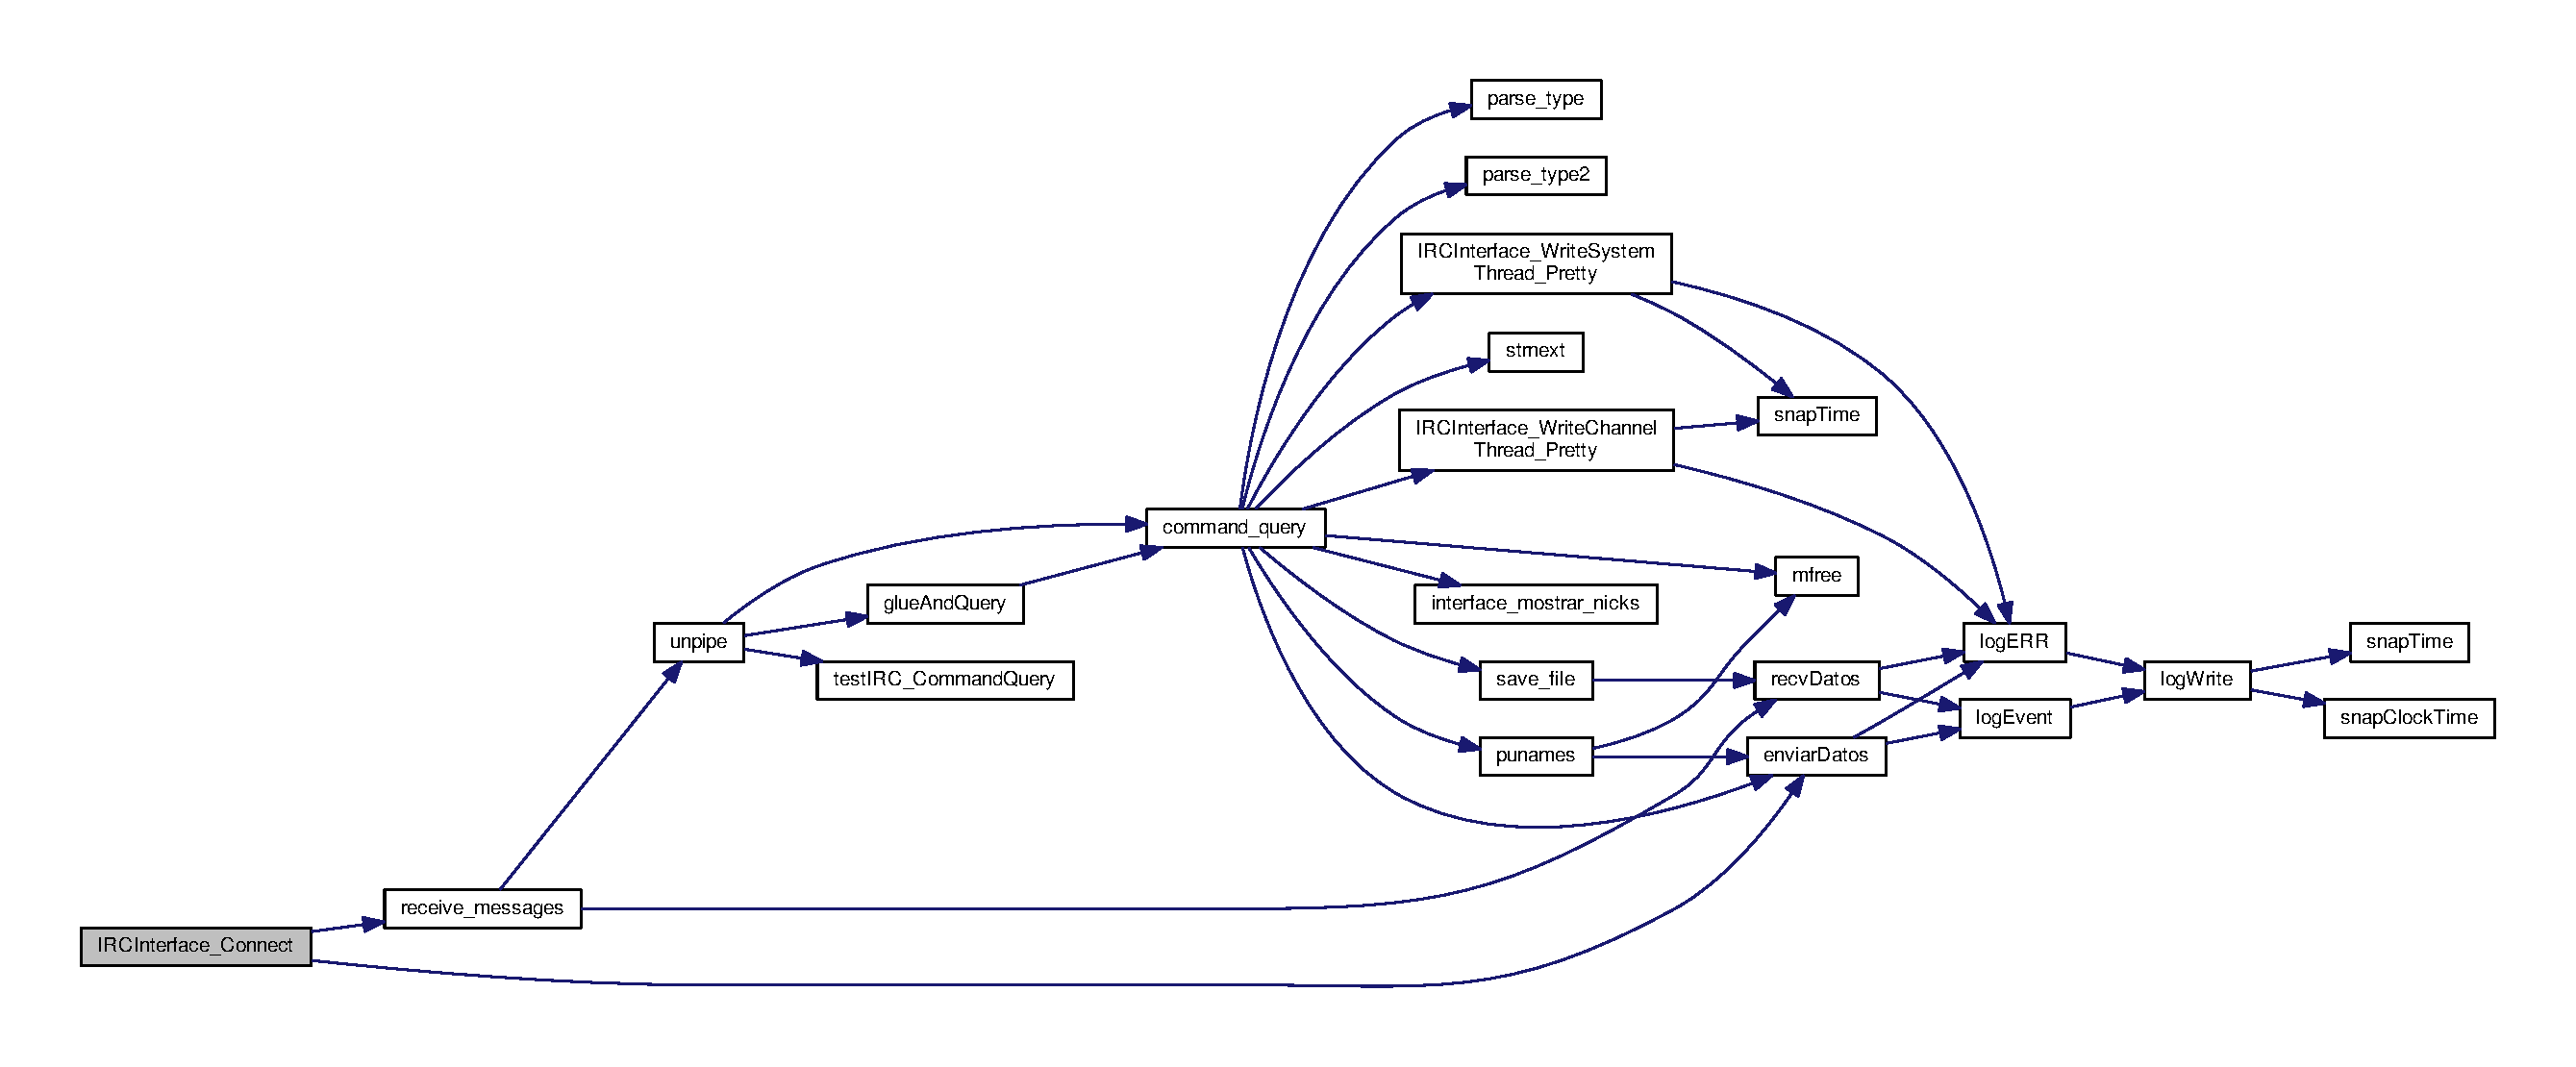
\includegraphics[width=350pt]{xchat2_8c_aed072f4ce0d6e90697d4d6eb0278a2ad_cgraph}
\end{center}
\end{figure}


\hypertarget{xchat2_8c_a3e67ee0cd384b524d57fda14593dce8e}{\index{xchat2.\-c@{xchat2.\-c}!I\-R\-C\-Interface\-\_\-\-Deactivate\-Channel\-Key@{I\-R\-C\-Interface\-\_\-\-Deactivate\-Channel\-Key}}
\index{I\-R\-C\-Interface\-\_\-\-Deactivate\-Channel\-Key@{I\-R\-C\-Interface\-\_\-\-Deactivate\-Channel\-Key}!xchat2.c@{xchat2.\-c}}
\subsubsection[{I\-R\-C\-Interface\-\_\-\-Deactivate\-Channel\-Key}]{\setlength{\rightskip}{0pt plus 5cm}void I\-R\-C\-Interface\-\_\-\-Deactivate\-Channel\-Key (
\begin{DoxyParamCaption}
\item[{char $\ast$}]{channel}
\end{DoxyParamCaption}
)}}\label{xchat2_8c_a3e67ee0cd384b524d57fda14593dce8e}

\begin{DoxyCode}
1787 \{
1788         g\_print(\hyperlink{types_8h_add9307de87f38e77d336751e305886f6}{BLU} \textcolor{stringliteral}{"\(\backslash\)nIRCInterface\_DeactivateChannelKey(char *channel) call\(\backslash\)n"} 
      \hyperlink{types_8h_ab702106cf3b3e96750b6845ded4e0299}{RESET});
1789 
1790         \textcolor{keywordflow}{if} (\hyperlink{aux__functions_8h_a06340d30a60b297a60b17841767fad85}{changeMode}(channel, NULL, \textcolor{stringliteral}{"-k"}) != \hyperlink{daemon_8h_aba51915c87d64af47fb1cc59348961c9}{OK})
1791                 g\_print(\hyperlink{types_8h_a8d23feea868a983c8c2b661e1e16972f}{RED} \textcolor{stringliteral}{"ERROR - In IRCInterface\_DeactivateChannelKey: Error en changeMode, devolvió
       ERR\(\backslash\)n"} \hyperlink{types_8h_ab702106cf3b3e96750b6845ded4e0299}{RESET});
1792 \}
\end{DoxyCode}


Here is the call graph for this function\-:
\nopagebreak
\begin{figure}[H]
\begin{center}
\leavevmode
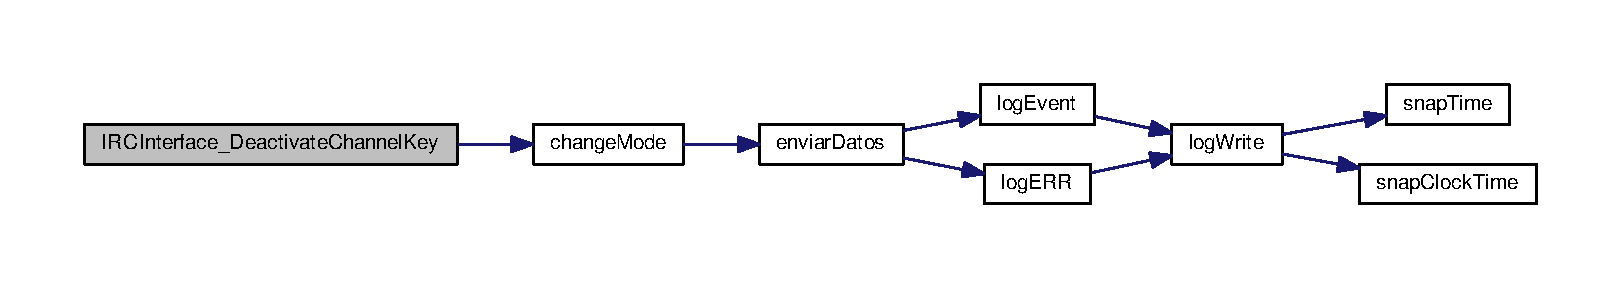
\includegraphics[width=350pt]{xchat2_8c_a3e67ee0cd384b524d57fda14593dce8e_cgraph}
\end{center}
\end{figure}


\hypertarget{xchat2_8c_a638b1535f4ecbc9a6affb2df2a6a946e}{\index{xchat2.\-c@{xchat2.\-c}!I\-R\-C\-Interface\-\_\-\-Deactivate\-External\-Messages@{I\-R\-C\-Interface\-\_\-\-Deactivate\-External\-Messages}}
\index{I\-R\-C\-Interface\-\_\-\-Deactivate\-External\-Messages@{I\-R\-C\-Interface\-\_\-\-Deactivate\-External\-Messages}!xchat2.c@{xchat2.\-c}}
\subsubsection[{I\-R\-C\-Interface\-\_\-\-Deactivate\-External\-Messages}]{\setlength{\rightskip}{0pt plus 5cm}void I\-R\-C\-Interface\-\_\-\-Deactivate\-External\-Messages (
\begin{DoxyParamCaption}
\item[{char $\ast$}]{channel}
\end{DoxyParamCaption}
)}}\label{xchat2_8c_a638b1535f4ecbc9a6affb2df2a6a946e}

\begin{DoxyCode}
1825 \{
1826         g\_print(\hyperlink{types_8h_add9307de87f38e77d336751e305886f6}{BLU} \textcolor{stringliteral}{"\(\backslash\)nIRCInterface\_DeactivateExternalMessages(char *channel) call\(\backslash\)n"} 
      \hyperlink{types_8h_ab702106cf3b3e96750b6845ded4e0299}{RESET});
1827 
1828         \textcolor{keywordflow}{if} (\hyperlink{aux__functions_8h_a06340d30a60b297a60b17841767fad85}{changeMode}(channel, NULL, \textcolor{stringliteral}{"-n"}) != \hyperlink{daemon_8h_aba51915c87d64af47fb1cc59348961c9}{OK})
1829                 g\_print(\hyperlink{types_8h_a8d23feea868a983c8c2b661e1e16972f}{RED} \textcolor{stringliteral}{"ERROR - In IRCInterface\_DeactivateExternalMessages: Error en changeMode,
       devolvió ERR\(\backslash\)n"} \hyperlink{types_8h_ab702106cf3b3e96750b6845ded4e0299}{RESET});
1830 \}
\end{DoxyCode}


Here is the call graph for this function\-:
\nopagebreak
\begin{figure}[H]
\begin{center}
\leavevmode
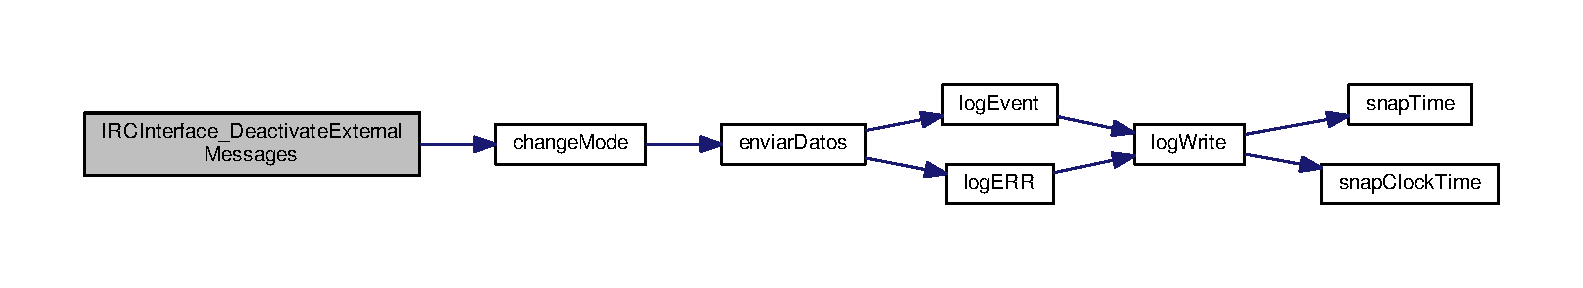
\includegraphics[width=350pt]{xchat2_8c_a638b1535f4ecbc9a6affb2df2a6a946e_cgraph}
\end{center}
\end{figure}


\hypertarget{xchat2_8c_a9ba4e98a3729737aa63ebec54ba4e894}{\index{xchat2.\-c@{xchat2.\-c}!I\-R\-C\-Interface\-\_\-\-Deactivate\-Invite@{I\-R\-C\-Interface\-\_\-\-Deactivate\-Invite}}
\index{I\-R\-C\-Interface\-\_\-\-Deactivate\-Invite@{I\-R\-C\-Interface\-\_\-\-Deactivate\-Invite}!xchat2.c@{xchat2.\-c}}
\subsubsection[{I\-R\-C\-Interface\-\_\-\-Deactivate\-Invite}]{\setlength{\rightskip}{0pt plus 5cm}void I\-R\-C\-Interface\-\_\-\-Deactivate\-Invite (
\begin{DoxyParamCaption}
\item[{char $\ast$}]{channel}
\end{DoxyParamCaption}
)}}\label{xchat2_8c_a9ba4e98a3729737aa63ebec54ba4e894}

\begin{DoxyCode}
1863 \{
1864         g\_print(\hyperlink{types_8h_add9307de87f38e77d336751e305886f6}{BLU} \textcolor{stringliteral}{"\(\backslash\)nIRCInterface\_DeactivateInvite(char *channel) call\(\backslash\)n"} 
      \hyperlink{types_8h_ab702106cf3b3e96750b6845ded4e0299}{RESET});
1865 
1866         \textcolor{keywordflow}{if} (\hyperlink{aux__functions_8h_a06340d30a60b297a60b17841767fad85}{changeMode}(channel, NULL, \textcolor{stringliteral}{"-i"}) != \hyperlink{daemon_8h_aba51915c87d64af47fb1cc59348961c9}{OK})
1867                 g\_print(\hyperlink{types_8h_a8d23feea868a983c8c2b661e1e16972f}{RED} \textcolor{stringliteral}{"ERROR - In IRCInterface\_DeactivateInvite: Error en changeMode, devolvió ERR
      \(\backslash\)n"} \hyperlink{types_8h_ab702106cf3b3e96750b6845ded4e0299}{RESET});
1868 \}
\end{DoxyCode}


Here is the call graph for this function\-:
\nopagebreak
\begin{figure}[H]
\begin{center}
\leavevmode
\includegraphics[width=350pt]{xchat2_8c_a9ba4e98a3729737aa63ebec54ba4e894_cgraph}
\end{center}
\end{figure}


\hypertarget{xchat2_8c_ab760e8144b38f6c14bd809d157cee5d4}{\index{xchat2.\-c@{xchat2.\-c}!I\-R\-C\-Interface\-\_\-\-Deactivate\-Moderated@{I\-R\-C\-Interface\-\_\-\-Deactivate\-Moderated}}
\index{I\-R\-C\-Interface\-\_\-\-Deactivate\-Moderated@{I\-R\-C\-Interface\-\_\-\-Deactivate\-Moderated}!xchat2.c@{xchat2.\-c}}
\subsubsection[{I\-R\-C\-Interface\-\_\-\-Deactivate\-Moderated}]{\setlength{\rightskip}{0pt plus 5cm}void I\-R\-C\-Interface\-\_\-\-Deactivate\-Moderated (
\begin{DoxyParamCaption}
\item[{char $\ast$}]{channel}
\end{DoxyParamCaption}
)}}\label{xchat2_8c_ab760e8144b38f6c14bd809d157cee5d4}

\begin{DoxyCode}
1901 \{
1902         g\_print(\hyperlink{types_8h_add9307de87f38e77d336751e305886f6}{BLU} \textcolor{stringliteral}{"\(\backslash\)nIRCInterface\_DeactivateModerated(char *channel) call\(\backslash\)n"} 
      \hyperlink{types_8h_ab702106cf3b3e96750b6845ded4e0299}{RESET});
1903 
1904         \textcolor{keywordflow}{if} (\hyperlink{aux__functions_8h_a06340d30a60b297a60b17841767fad85}{changeMode}(channel, NULL, \textcolor{stringliteral}{"-m"}) != \hyperlink{daemon_8h_aba51915c87d64af47fb1cc59348961c9}{OK})
1905                 g\_print(\hyperlink{types_8h_a8d23feea868a983c8c2b661e1e16972f}{RED} \textcolor{stringliteral}{"ERROR - In IRCInterface\_DeactivateModerated: Error en changeMode, devolvió
       ERR\(\backslash\)n"} \hyperlink{types_8h_ab702106cf3b3e96750b6845ded4e0299}{RESET});
1906 \}
\end{DoxyCode}


Here is the call graph for this function\-:
\nopagebreak
\begin{figure}[H]
\begin{center}
\leavevmode
\includegraphics[width=350pt]{xchat2_8c_ab760e8144b38f6c14bd809d157cee5d4_cgraph}
\end{center}
\end{figure}


\hypertarget{xchat2_8c_a92c8cfbe2e14e19277e1c97d11719e80}{\index{xchat2.\-c@{xchat2.\-c}!I\-R\-C\-Interface\-\_\-\-Deactivate\-Nicks\-Limit@{I\-R\-C\-Interface\-\_\-\-Deactivate\-Nicks\-Limit}}
\index{I\-R\-C\-Interface\-\_\-\-Deactivate\-Nicks\-Limit@{I\-R\-C\-Interface\-\_\-\-Deactivate\-Nicks\-Limit}!xchat2.c@{xchat2.\-c}}
\subsubsection[{I\-R\-C\-Interface\-\_\-\-Deactivate\-Nicks\-Limit}]{\setlength{\rightskip}{0pt plus 5cm}void I\-R\-C\-Interface\-\_\-\-Deactivate\-Nicks\-Limit (
\begin{DoxyParamCaption}
\item[{char $\ast$}]{channel}
\end{DoxyParamCaption}
)}}\label{xchat2_8c_a92c8cfbe2e14e19277e1c97d11719e80}

\begin{DoxyCode}
1939 \{
1940         g\_print(\hyperlink{types_8h_add9307de87f38e77d336751e305886f6}{BLU} \textcolor{stringliteral}{"\(\backslash\)nIRCInterface\_DeactivateNicksLimit(char *channel) call\(\backslash\)n"} 
      \hyperlink{types_8h_ab702106cf3b3e96750b6845ded4e0299}{RESET});
1941 
1942         \textcolor{keywordflow}{if} (\hyperlink{aux__functions_8h_a06340d30a60b297a60b17841767fad85}{changeMode}(channel, NULL, \textcolor{stringliteral}{"-l"}) != \hyperlink{daemon_8h_aba51915c87d64af47fb1cc59348961c9}{OK})
1943                 g\_print(\hyperlink{types_8h_a8d23feea868a983c8c2b661e1e16972f}{RED} \textcolor{stringliteral}{"ERROR - In IRCInterface\_DeactivateNicksLimit: Error en changeMode, devolvió
       ERR\(\backslash\)n"} \hyperlink{types_8h_ab702106cf3b3e96750b6845ded4e0299}{RESET});
1944 \}
\end{DoxyCode}


Here is the call graph for this function\-:
\nopagebreak
\begin{figure}[H]
\begin{center}
\leavevmode
\includegraphics[width=350pt]{xchat2_8c_a92c8cfbe2e14e19277e1c97d11719e80_cgraph}
\end{center}
\end{figure}


\hypertarget{xchat2_8c_a8a6141803691ba327f11ba763ad075d4}{\index{xchat2.\-c@{xchat2.\-c}!I\-R\-C\-Interface\-\_\-\-Deactivate\-Private@{I\-R\-C\-Interface\-\_\-\-Deactivate\-Private}}
\index{I\-R\-C\-Interface\-\_\-\-Deactivate\-Private@{I\-R\-C\-Interface\-\_\-\-Deactivate\-Private}!xchat2.c@{xchat2.\-c}}
\subsubsection[{I\-R\-C\-Interface\-\_\-\-Deactivate\-Private}]{\setlength{\rightskip}{0pt plus 5cm}void I\-R\-C\-Interface\-\_\-\-Deactivate\-Private (
\begin{DoxyParamCaption}
\item[{char $\ast$}]{channel}
\end{DoxyParamCaption}
)}}\label{xchat2_8c_a8a6141803691ba327f11ba763ad075d4}

\begin{DoxyCode}
1979 \{
1980         g\_print(\hyperlink{types_8h_add9307de87f38e77d336751e305886f6}{BLU} \textcolor{stringliteral}{"\(\backslash\)nIRCInterface\_DeactivatePrivate(char *channel) call\(\backslash\)n"} 
      \hyperlink{types_8h_ab702106cf3b3e96750b6845ded4e0299}{RESET});
1981 
1982         \textcolor{keywordflow}{if} (\hyperlink{aux__functions_8h_a06340d30a60b297a60b17841767fad85}{changeMode}(channel, NULL, \textcolor{stringliteral}{"-p"}) != \hyperlink{daemon_8h_aba51915c87d64af47fb1cc59348961c9}{OK})
1983                 g\_print(\hyperlink{types_8h_a8d23feea868a983c8c2b661e1e16972f}{RED} \textcolor{stringliteral}{"ERROR - In IRCInterface\_DeactivatePrivate: Error en changeMode, devolvió
       ERR\(\backslash\)n"} \hyperlink{types_8h_ab702106cf3b3e96750b6845ded4e0299}{RESET});
1984 \}
\end{DoxyCode}


Here is the call graph for this function\-:
\nopagebreak
\begin{figure}[H]
\begin{center}
\leavevmode
\includegraphics[width=350pt]{xchat2_8c_a8a6141803691ba327f11ba763ad075d4_cgraph}
\end{center}
\end{figure}


\hypertarget{xchat2_8c_a5a57541a950f8c2c40b4b44c32b28ed9}{\index{xchat2.\-c@{xchat2.\-c}!I\-R\-C\-Interface\-\_\-\-Deactivate\-Protect\-Topic@{I\-R\-C\-Interface\-\_\-\-Deactivate\-Protect\-Topic}}
\index{I\-R\-C\-Interface\-\_\-\-Deactivate\-Protect\-Topic@{I\-R\-C\-Interface\-\_\-\-Deactivate\-Protect\-Topic}!xchat2.c@{xchat2.\-c}}
\subsubsection[{I\-R\-C\-Interface\-\_\-\-Deactivate\-Protect\-Topic}]{\setlength{\rightskip}{0pt plus 5cm}void I\-R\-C\-Interface\-\_\-\-Deactivate\-Protect\-Topic (
\begin{DoxyParamCaption}
\item[{char $\ast$}]{channel}
\end{DoxyParamCaption}
)}}\label{xchat2_8c_a5a57541a950f8c2c40b4b44c32b28ed9}

\begin{DoxyCode}
2017 \{
2018         g\_print(\hyperlink{types_8h_add9307de87f38e77d336751e305886f6}{BLU} \textcolor{stringliteral}{"\(\backslash\)nIRCInterface\_DeactivateProtectTopic(char *channel) call\(\backslash\)n"} 
      \hyperlink{types_8h_ab702106cf3b3e96750b6845ded4e0299}{RESET});
2019 
2020         \textcolor{keywordflow}{if} (\hyperlink{aux__functions_8h_a06340d30a60b297a60b17841767fad85}{changeMode}(channel, NULL, \textcolor{stringliteral}{"-t"}) != \hyperlink{daemon_8h_aba51915c87d64af47fb1cc59348961c9}{OK})
2021                 g\_print(\hyperlink{types_8h_a8d23feea868a983c8c2b661e1e16972f}{RED} \textcolor{stringliteral}{"ERROR - In IRCInterface\_DeactivateProtectTopic: Error en changeMode,
       devolvió ERR\(\backslash\)n"} \hyperlink{types_8h_ab702106cf3b3e96750b6845ded4e0299}{RESET});
2022 \}
\end{DoxyCode}


Here is the call graph for this function\-:
\nopagebreak
\begin{figure}[H]
\begin{center}
\leavevmode
\includegraphics[width=350pt]{xchat2_8c_a5a57541a950f8c2c40b4b44c32b28ed9_cgraph}
\end{center}
\end{figure}


\hypertarget{xchat2_8c_a4956427664cabc7d5b2bd1589a207324}{\index{xchat2.\-c@{xchat2.\-c}!I\-R\-C\-Interface\-\_\-\-Deactivate\-Secret@{I\-R\-C\-Interface\-\_\-\-Deactivate\-Secret}}
\index{I\-R\-C\-Interface\-\_\-\-Deactivate\-Secret@{I\-R\-C\-Interface\-\_\-\-Deactivate\-Secret}!xchat2.c@{xchat2.\-c}}
\subsubsection[{I\-R\-C\-Interface\-\_\-\-Deactivate\-Secret}]{\setlength{\rightskip}{0pt plus 5cm}void I\-R\-C\-Interface\-\_\-\-Deactivate\-Secret (
\begin{DoxyParamCaption}
\item[{char $\ast$}]{channel}
\end{DoxyParamCaption}
)}}\label{xchat2_8c_a4956427664cabc7d5b2bd1589a207324}

\begin{DoxyCode}
2055 \{
2056         g\_print(\hyperlink{types_8h_add9307de87f38e77d336751e305886f6}{BLU} \textcolor{stringliteral}{"\(\backslash\)nIRCInterface\_DeactivateSecret(char *channel) call\(\backslash\)n"} 
      \hyperlink{types_8h_ab702106cf3b3e96750b6845ded4e0299}{RESET});
2057 
2058         \textcolor{keywordflow}{if} (\hyperlink{aux__functions_8h_a06340d30a60b297a60b17841767fad85}{changeMode}(channel, NULL, \textcolor{stringliteral}{"-s"}) != \hyperlink{daemon_8h_aba51915c87d64af47fb1cc59348961c9}{OK})
2059                 g\_print(\hyperlink{types_8h_a8d23feea868a983c8c2b661e1e16972f}{RED} \textcolor{stringliteral}{"ERROR - In IRCInterface\_DeactivateSecret: Error en changeMode, devolvió ERR
      \(\backslash\)n"} \hyperlink{types_8h_ab702106cf3b3e96750b6845ded4e0299}{RESET});
2060 \}
\end{DoxyCode}


Here is the call graph for this function\-:
\nopagebreak
\begin{figure}[H]
\begin{center}
\leavevmode
\includegraphics[width=350pt]{xchat2_8c_a4956427664cabc7d5b2bd1589a207324_cgraph}
\end{center}
\end{figure}


\hypertarget{xchat2_8c_a8bf0424ef7f845be79a056e9aed56fe2}{\index{xchat2.\-c@{xchat2.\-c}!I\-R\-C\-Interface\-\_\-\-Disconnect\-Server@{I\-R\-C\-Interface\-\_\-\-Disconnect\-Server}}
\index{I\-R\-C\-Interface\-\_\-\-Disconnect\-Server@{I\-R\-C\-Interface\-\_\-\-Disconnect\-Server}!xchat2.c@{xchat2.\-c}}
\subsubsection[{I\-R\-C\-Interface\-\_\-\-Disconnect\-Server}]{\setlength{\rightskip}{0pt plus 5cm}boolean I\-R\-C\-Interface\-\_\-\-Disconnect\-Server (
\begin{DoxyParamCaption}
\item[{char $\ast$}]{server, }
\item[{int}]{port}
\end{DoxyParamCaption}
)}}\label{xchat2_8c_a8bf0424ef7f845be79a056e9aed56fe2}

\begin{DoxyCode}
2097 \{
2098         g\_print(\hyperlink{types_8h_add9307de87f38e77d336751e305886f6}{BLU} \textcolor{stringliteral}{"\(\backslash\)nIRCInterface\_DisconnectServer(char *server, int port) call\(\backslash\)n"} 
      \hyperlink{types_8h_ab702106cf3b3e96750b6845ded4e0299}{RESET});
2099 
2100         \hyperlink{user__commands_8h_ad738a7d361fe18d7774bab370a4454a8}{puquit}(NULL);
2101 
2102         \textcolor{keywordflow}{return} TRUE;
2103 \}
\end{DoxyCode}


Here is the call graph for this function\-:
\nopagebreak
\begin{figure}[H]
\begin{center}
\leavevmode
\includegraphics[width=350pt]{xchat2_8c_a8bf0424ef7f845be79a056e9aed56fe2_cgraph}
\end{center}
\end{figure}


\hypertarget{xchat2_8c_ab431412191716f751461f94d613ffdab}{\index{xchat2.\-c@{xchat2.\-c}!I\-R\-C\-Interface\-\_\-\-Exit\-Audio\-Chat@{I\-R\-C\-Interface\-\_\-\-Exit\-Audio\-Chat}}
\index{I\-R\-C\-Interface\-\_\-\-Exit\-Audio\-Chat@{I\-R\-C\-Interface\-\_\-\-Exit\-Audio\-Chat}!xchat2.c@{xchat2.\-c}}
\subsubsection[{I\-R\-C\-Interface\-\_\-\-Exit\-Audio\-Chat}]{\setlength{\rightskip}{0pt plus 5cm}boolean I\-R\-C\-Interface\-\_\-\-Exit\-Audio\-Chat (
\begin{DoxyParamCaption}
\item[{char $\ast$}]{nick}
\end{DoxyParamCaption}
)}}\label{xchat2_8c_ab431412191716f751461f94d613ffdab}

\begin{DoxyCode}
2141 \{
2142         g\_print(\hyperlink{types_8h_add9307de87f38e77d336751e305886f6}{BLU} \textcolor{stringliteral}{"\(\backslash\)nIRCInterface\_ExitAudioChat(char *nick) call\(\backslash\)n"} \hyperlink{types_8h_ab702106cf3b3e96750b6845ded4e0299}{RESET});
2143         \textcolor{keywordflow}{return} TRUE;
2144 \}
\end{DoxyCode}
\hypertarget{xchat2_8c_ae075029bb55e8b995f22beb0810674f4}{\index{xchat2.\-c@{xchat2.\-c}!I\-R\-C\-Interface\-\_\-\-Give\-Op@{I\-R\-C\-Interface\-\_\-\-Give\-Op}}
\index{I\-R\-C\-Interface\-\_\-\-Give\-Op@{I\-R\-C\-Interface\-\_\-\-Give\-Op}!xchat2.c@{xchat2.\-c}}
\subsubsection[{I\-R\-C\-Interface\-\_\-\-Give\-Op}]{\setlength{\rightskip}{0pt plus 5cm}void I\-R\-C\-Interface\-\_\-\-Give\-Op (
\begin{DoxyParamCaption}
\item[{char $\ast$}]{channel, }
\item[{char $\ast$}]{nick}
\end{DoxyParamCaption}
)}}\label{xchat2_8c_ae075029bb55e8b995f22beb0810674f4}

\begin{DoxyCode}
2179 \{
2180         g\_print(\hyperlink{types_8h_add9307de87f38e77d336751e305886f6}{BLU} \textcolor{stringliteral}{"\(\backslash\)nIRCInterface\_GiveOp(char *channel, char *nick) call\(\backslash\)n"} 
      \hyperlink{types_8h_ab702106cf3b3e96750b6845ded4e0299}{RESET});
2181 
2182         \textcolor{keywordflow}{if} (\hyperlink{aux__functions_8h_a06340d30a60b297a60b17841767fad85}{changeMode}(channel, nick, \textcolor{stringliteral}{"+o"}) != \hyperlink{daemon_8h_aba51915c87d64af47fb1cc59348961c9}{OK})
2183                 g\_print(\hyperlink{types_8h_a8d23feea868a983c8c2b661e1e16972f}{RED} \textcolor{stringliteral}{"ERROR - In IRCInterface\_GiveOp: Error en changeMode, devolvió ERR\(\backslash\)n"} 
      \hyperlink{types_8h_ab702106cf3b3e96750b6845ded4e0299}{RESET});
2184 \}
\end{DoxyCode}


Here is the call graph for this function\-:
\nopagebreak
\begin{figure}[H]
\begin{center}
\leavevmode
\includegraphics[width=350pt]{xchat2_8c_ae075029bb55e8b995f22beb0810674f4_cgraph}
\end{center}
\end{figure}


\hypertarget{xchat2_8c_ae9effb4bdaf4a2cdf2dd9edbeb90b430}{\index{xchat2.\-c@{xchat2.\-c}!I\-R\-C\-Interface\-\_\-\-Give\-Voice@{I\-R\-C\-Interface\-\_\-\-Give\-Voice}}
\index{I\-R\-C\-Interface\-\_\-\-Give\-Voice@{I\-R\-C\-Interface\-\_\-\-Give\-Voice}!xchat2.c@{xchat2.\-c}}
\subsubsection[{I\-R\-C\-Interface\-\_\-\-Give\-Voice}]{\setlength{\rightskip}{0pt plus 5cm}void I\-R\-C\-Interface\-\_\-\-Give\-Voice (
\begin{DoxyParamCaption}
\item[{char $\ast$}]{channel, }
\item[{char $\ast$}]{nick}
\end{DoxyParamCaption}
)}}\label{xchat2_8c_ae9effb4bdaf4a2cdf2dd9edbeb90b430}

\begin{DoxyCode}
2219 \{
2220         g\_print(\hyperlink{types_8h_add9307de87f38e77d336751e305886f6}{BLU} \textcolor{stringliteral}{"\(\backslash\)nIRCInterface\_GiveVoice(char *channel, char *nick) call\(\backslash\)n"} 
      \hyperlink{types_8h_ab702106cf3b3e96750b6845ded4e0299}{RESET});
2221 
2222         \textcolor{keywordflow}{if} (\hyperlink{aux__functions_8h_a06340d30a60b297a60b17841767fad85}{changeMode}(channel, nick, \textcolor{stringliteral}{"+v"}) != \hyperlink{daemon_8h_aba51915c87d64af47fb1cc59348961c9}{OK})
2223                 g\_print(\hyperlink{types_8h_a8d23feea868a983c8c2b661e1e16972f}{RED} \textcolor{stringliteral}{"ERROR - In IRCInterface\_GiveOp: Error en changeMode, devolvió ERR\(\backslash\)n"} 
      \hyperlink{types_8h_ab702106cf3b3e96750b6845ded4e0299}{RESET});
2224 \}
\end{DoxyCode}


Here is the call graph for this function\-:
\nopagebreak
\begin{figure}[H]
\begin{center}
\leavevmode
\includegraphics[width=350pt]{xchat2_8c_ae9effb4bdaf4a2cdf2dd9edbeb90b430_cgraph}
\end{center}
\end{figure}


\hypertarget{xchat2_8c_a7adfea400a96160585f86179bafb055f}{\index{xchat2.\-c@{xchat2.\-c}!I\-R\-C\-Interface\-\_\-\-Kick\-Nick@{I\-R\-C\-Interface\-\_\-\-Kick\-Nick}}
\index{I\-R\-C\-Interface\-\_\-\-Kick\-Nick@{I\-R\-C\-Interface\-\_\-\-Kick\-Nick}!xchat2.c@{xchat2.\-c}}
\subsubsection[{I\-R\-C\-Interface\-\_\-\-Kick\-Nick}]{\setlength{\rightskip}{0pt plus 5cm}void I\-R\-C\-Interface\-\_\-\-Kick\-Nick (
\begin{DoxyParamCaption}
\item[{char $\ast$}]{channel, }
\item[{char $\ast$}]{nick}
\end{DoxyParamCaption}
)}}\label{xchat2_8c_a7adfea400a96160585f86179bafb055f}

\begin{DoxyCode}
2259 \{
2260         g\_print(\hyperlink{types_8h_add9307de87f38e77d336751e305886f6}{BLU} \textcolor{stringliteral}{"\(\backslash\)nIRCInterface\_KickNick(char *channel, char *nick) call\(\backslash\)n"} 
      \hyperlink{types_8h_ab702106cf3b3e96750b6845ded4e0299}{RESET});
2261 
2262         \textcolor{keywordtype}{int} ret = -1;
2263         \textcolor{keywordtype}{char} *command=NULL;
2264 
2265         \textcolor{comment}{//long IRCMsg\_Kick (char **command, char *prefix, char * channel, char *user, char *comment)}
2266         ret = IRCMsg\_Kick (&command, NULL, channel, nick, \textcolor{stringliteral}{"Te han echado del canal."});
2267         \textcolor{keywordflow}{if}(ret != IRC\_OK)\{
2268                 g\_print(\hyperlink{types_8h_a8d23feea868a983c8c2b661e1e16972f}{RED} \textcolor{stringliteral}{"ERROR - In IRCInterface\_KickNick : Error en IRCMsg\_Kick, no devolvio IRC\_OK
      \(\backslash\)n"} \hyperlink{types_8h_ab702106cf3b3e96750b6845ded4e0299}{RESET});
2269                 \textcolor{keywordflow}{return};
2270         \}
2271         ret = \hyperlink{conexion__tcp_8h_ab9468ce1338cfca5736ab407ba155f55}{enviarDatos}(\hyperlink{xchat2_8c_acd63fb8dbd9439219e2db08dfc173aa0}{sockfd\_user}, command, strlen(command));
2272         \textcolor{keywordflow}{if}(ret == \hyperlink{types_8h_a735563036dced0b7d6cc98f97ea4978b}{ERR})\{
2273                 g\_print(\hyperlink{types_8h_a8d23feea868a983c8c2b661e1e16972f}{RED} \textcolor{stringliteral}{"ERROR - In IRCInterface\_KickNick: enviarDatos devolvio ERR\(\backslash\)n"} 
      \hyperlink{types_8h_ab702106cf3b3e96750b6845ded4e0299}{RESET});
2274                 \textcolor{keywordflow}{return};
2275         \}
2276         IRCInterface\_PlaneRegisterOutMessage(command);
2277         free(command);  
2278 \}
\end{DoxyCode}


Here is the call graph for this function\-:
\nopagebreak
\begin{figure}[H]
\begin{center}
\leavevmode
\includegraphics[width=350pt]{xchat2_8c_a7adfea400a96160585f86179bafb055f_cgraph}
\end{center}
\end{figure}


\hypertarget{xchat2_8c_a214e10b19c8be028fb35d2a7abf3f798}{\index{xchat2.\-c@{xchat2.\-c}!I\-R\-C\-Interface\-\_\-\-New\-Command\-Text@{I\-R\-C\-Interface\-\_\-\-New\-Command\-Text}}
\index{I\-R\-C\-Interface\-\_\-\-New\-Command\-Text@{I\-R\-C\-Interface\-\_\-\-New\-Command\-Text}!xchat2.c@{xchat2.\-c}}
\subsubsection[{I\-R\-C\-Interface\-\_\-\-New\-Command\-Text}]{\setlength{\rightskip}{0pt plus 5cm}void I\-R\-C\-Interface\-\_\-\-New\-Command\-Text (
\begin{DoxyParamCaption}
\item[{char $\ast$}]{command}
\end{DoxyParamCaption}
)}}\label{xchat2_8c_a214e10b19c8be028fb35d2a7abf3f798}

\begin{DoxyCode}
2313 \{
2314         g\_print(\hyperlink{types_8h_add9307de87f38e77d336751e305886f6}{BLU} \textcolor{stringliteral}{"\(\backslash\)n[callback] IRCInterface\_NewCommandText(char *command) call\(\backslash\)n"} 
      \hyperlink{types_8h_ab702106cf3b3e96750b6845ded4e0299}{RESET});
2315 
2316         \textcolor{keywordtype}{int} num\_comando = -1, ret;
2317         \textcolor{keywordtype}{char} *comando = NULL;
2318         \textcolor{keywordtype}{char} *prefix = NULL;
2319         \textcolor{comment}{//pthread\_t tid;}
2320         \textcolor{comment}{//IRCInterface\_PlaneRegisterInMessage(command);}
2321         \textcolor{comment}{//IRCInterface\_WriteSystem(nick\_user, command);}
2322 
2323         \textcolor{keywordflow}{if}(command[0] != \textcolor{charliteral}{'/'})\{\textcolor{comment}{//mensaje a grupo o nick directamente}
2324                 \hyperlink{xchat2_8c_a568595cf14231c912fd7ab15a324bd16}{active\_channel} = IRCInterface\_ActiveChannelName();
2325                 g\_print(\textcolor{stringliteral}{"Active\_channel: %s\(\backslash\)n"}, \hyperlink{xchat2_8c_a568595cf14231c912fd7ab15a324bd16}{active\_channel});
2326 
2327                 \textcolor{comment}{//   long IRCMsg\_Privmsg (char **command, char *prefix, char * msgtarget, char *msg)}
2328                 ret = IRCMsg\_Privmsg (&comando, prefix, \hyperlink{xchat2_8c_a568595cf14231c912fd7ab15a324bd16}{active\_channel}, command);
2329                 \textcolor{keywordflow}{if}(ret == \hyperlink{types_8h_a735563036dced0b7d6cc98f97ea4978b}{ERR})\{
2330                         g\_print(\hyperlink{types_8h_a8d23feea868a983c8c2b661e1e16972f}{RED} \textcolor{stringliteral}{"ERROR - In IRCInterface\_NewCommandText: IRCMsg\_Privmsg devolvio
       error\(\backslash\)n"} \hyperlink{types_8h_ab702106cf3b3e96750b6845ded4e0299}{RESET});
2331                         \textcolor{keywordflow}{return};
2332                 \}
2333                 g\_print(\textcolor{stringliteral}{"\(\backslash\)t Mensaje a enviar IRCMsg\_Privmsg: %s \(\backslash\)n"},comando);
2334 
2335                 ret = \hyperlink{conexion__tcp_8h_ab9468ce1338cfca5736ab407ba155f55}{enviarDatos}(\hyperlink{xchat2_8c_acd63fb8dbd9439219e2db08dfc173aa0}{sockfd\_user},comando, strlen(comando));
2336                 \textcolor{keywordflow}{if}(ret < 0)\{
2337                         g\_print(\hyperlink{types_8h_a8d23feea868a983c8c2b661e1e16972f}{RED} \textcolor{stringliteral}{"ERROR - In IRCInterface\_NewCommandText: enviarDatos() devolvio
       error (ver secuencia en .log)\(\backslash\)n\(\backslash\)t\(\backslash\)tEl cliente se cerrará.\(\backslash\)n"} \hyperlink{types_8h_ab702106cf3b3e96750b6845ded4e0299}{RESET});
2338                         exit(1);
2339                 \}
2340                 \textcolor{keywordflow}{if}(ret == 0)\{ \textcolor{comment}{//timeout }
2341                         g\_print(\hyperlink{types_8h_a8d23feea868a983c8c2b661e1e16972f}{RED} \textcolor{stringliteral}{"ERROR - In IRCInterface\_NewCommandText: enviarDatos() mandó 0
       Bytes(ver secuencia en .log)\(\backslash\)n\(\backslash\)t\(\backslash\)t(Timeout de conexión probablemente)\(\backslash\)n"} \hyperlink{types_8h_ab702106cf3b3e96750b6845ded4e0299}{RESET});
2342                         exit(1);
2343                 \}
2344                 IRCInterface\_PlaneRegisterOutMessage(comando);
2345                 \textcolor{comment}{//No recibimos nada en este comando, los mensajes de otros usuarios los recibimos por otro
       hilo}
2346                 IRCInterface\_WriteChannel(\hyperlink{xchat2_8c_a568595cf14231c912fd7ab15a324bd16}{active\_channel}, 
      \hyperlink{xchat2_8c_a7e2f32e47f3780a66e19651d8e79bced}{nick\_user}, command);
2347                 \textcolor{keywordflow}{return};
2348         \}
2349 
2350         num\_comando = IRCUser\_CommandQuery (command);   
2351         g\_print(\hyperlink{types_8h_af54a5a977c0c499323d656315f008ee0}{MAG} \textcolor{stringliteral}{"\(\backslash\)n\(\backslash\)t>num\_comando -> array de funciones: %d \(\backslash\)n"} \hyperlink{types_8h_ab702106cf3b3e96750b6845ded4e0299}{RESET},num\_comando);
2352         \textcolor{keywordflow}{if} (num\_comando > 56)\{
2353                 g\_print(\hyperlink{types_8h_a96fac03c4ab3363f06a0328e0e53a40c}{YEL} \textcolor{stringliteral}{"\(\backslash\)nWARN - Comando de usuario no reconocido/no tiene asignado una funcion en
       el array.\(\backslash\)n"} \hyperlink{types_8h_ab702106cf3b3e96750b6845ded4e0299}{RESET});
2354                 \hyperlink{user__commands_8h_a05216fb56a43c8fa44b5bc726692b064}{pdefault}(command);
2355                 \textcolor{keywordflow}{return};
2356         \}
2357         \textcolor{keywordflow}{if} (\hyperlink{xchat2_8h_afe699fe3416e9bf2d3553e35d7a1dea2}{p\_array\_funciones}[num\_comando](command) == -1)\{
2358                 g\_print(\hyperlink{types_8h_a8d23feea868a983c8c2b661e1e16972f}{RED} \textcolor{stringliteral}{"ERROR - In IRCInterface\_NewCommandText: Error en p\_array\_funciones num: %d 
      \(\backslash\)n"} \hyperlink{types_8h_ab702106cf3b3e96750b6845ded4e0299}{RESET},num\_comando);
2359         \}
2360 \}
\end{DoxyCode}


Here is the call graph for this function\-:
\nopagebreak
\begin{figure}[H]
\begin{center}
\leavevmode
\includegraphics[width=350pt]{xchat2_8c_a214e10b19c8be028fb35d2a7abf3f798_cgraph}
\end{center}
\end{figure}


\hypertarget{xchat2_8c_a080cf34ff506481737f6d08af60ca92b}{\index{xchat2.\-c@{xchat2.\-c}!I\-R\-C\-Interface\-\_\-\-New\-Topic\-Enter@{I\-R\-C\-Interface\-\_\-\-New\-Topic\-Enter}}
\index{I\-R\-C\-Interface\-\_\-\-New\-Topic\-Enter@{I\-R\-C\-Interface\-\_\-\-New\-Topic\-Enter}!xchat2.c@{xchat2.\-c}}
\subsubsection[{I\-R\-C\-Interface\-\_\-\-New\-Topic\-Enter}]{\setlength{\rightskip}{0pt plus 5cm}void I\-R\-C\-Interface\-\_\-\-New\-Topic\-Enter (
\begin{DoxyParamCaption}
\item[{char $\ast$}]{topicdata}
\end{DoxyParamCaption}
)}}\label{xchat2_8c_a080cf34ff506481737f6d08af60ca92b}

\begin{DoxyCode}
2394 \{
2395         g\_print(\hyperlink{types_8h_add9307de87f38e77d336751e305886f6}{BLU} \textcolor{stringliteral}{"\(\backslash\)nIRCInterface\_NewTopicEnter(char *topicdata) call\(\backslash\)n"} 
      \hyperlink{types_8h_ab702106cf3b3e96750b6845ded4e0299}{RESET});
2396 
2397         \textcolor{keywordtype}{int} ret = -1;
2398         \textcolor{keywordtype}{char} *command=NULL;
2399 
2400         \textcolor{comment}{//long IRCMsg\_Topic (char **command, char *prefix, char * channel, char *topic)}
2401         \hyperlink{xchat2_8c_a568595cf14231c912fd7ab15a324bd16}{active\_channel} = IRCInterface\_ActiveChannelName();
2402         ret = IRCMsg\_Topic (&command, NULL, \hyperlink{xchat2_8c_a568595cf14231c912fd7ab15a324bd16}{active\_channel}, topicdata);
2403         \textcolor{keywordflow}{if}(ret != IRC\_OK)\{
2404                 g\_print(\hyperlink{types_8h_a8d23feea868a983c8c2b661e1e16972f}{RED} \textcolor{stringliteral}{"ERROR - In IRCInterface\_NewTopicEnter: IRCMsg\_Topic no devolvio IRC\_OK\(\backslash\)n"} 
      \hyperlink{types_8h_ab702106cf3b3e96750b6845ded4e0299}{RESET});
2405                 \textcolor{keywordflow}{return};
2406         \}
2407         ret = \hyperlink{conexion__tcp_8h_ab9468ce1338cfca5736ab407ba155f55}{enviarDatos}(\hyperlink{xchat2_8c_acd63fb8dbd9439219e2db08dfc173aa0}{sockfd\_user}, command, strlen(command));
2408         \textcolor{keywordflow}{if}(ret == \hyperlink{types_8h_a735563036dced0b7d6cc98f97ea4978b}{ERR})\{
2409                 g\_print(\hyperlink{types_8h_a8d23feea868a983c8c2b661e1e16972f}{RED} \textcolor{stringliteral}{"ERROR - In IRCInterface\_NewTopicEnter: enviarDatos devolvio ERR\(\backslash\)n"} 
      \hyperlink{types_8h_ab702106cf3b3e96750b6845ded4e0299}{RESET});
2410                 \textcolor{keywordflow}{return};
2411         \}
2412         IRCInterface\_PlaneRegisterOutMessage(command);
2413         free(command);  
2414 \}
\end{DoxyCode}


Here is the call graph for this function\-:
\nopagebreak
\begin{figure}[H]
\begin{center}
\leavevmode
\includegraphics[width=350pt]{xchat2_8c_a080cf34ff506481737f6d08af60ca92b_cgraph}
\end{center}
\end{figure}


\hypertarget{xchat2_8c_a100f1c87bb3b399a7284e62dd2e6172a}{\index{xchat2.\-c@{xchat2.\-c}!I\-R\-C\-Interface\-\_\-\-Send\-File@{I\-R\-C\-Interface\-\_\-\-Send\-File}}
\index{I\-R\-C\-Interface\-\_\-\-Send\-File@{I\-R\-C\-Interface\-\_\-\-Send\-File}!xchat2.c@{xchat2.\-c}}
\subsubsection[{I\-R\-C\-Interface\-\_\-\-Send\-File}]{\setlength{\rightskip}{0pt plus 5cm}boolean I\-R\-C\-Interface\-\_\-\-Send\-File (
\begin{DoxyParamCaption}
\item[{char $\ast$}]{filename, }
\item[{char $\ast$}]{nick, }
\item[{char $\ast$}]{data, }
\item[{long unsigned int}]{length}
\end{DoxyParamCaption}
)}}\label{xchat2_8c_a100f1c87bb3b399a7284e62dd2e6172a}

\begin{DoxyCode}
2456 \{
2457         g\_print(\hyperlink{types_8h_add9307de87f38e77d336751e305886f6}{BLU} \textcolor{stringliteral}{"\(\backslash\)nIRCInterface\_SendFile(char *filename, char *nick, char *data, long unsigned int
       length) call\(\backslash\)n"} \hyperlink{types_8h_ab702106cf3b3e96750b6845ded4e0299}{RESET});
2458         \textcolor{keywordflow}{return} TRUE;
2459 \}
\end{DoxyCode}
\hypertarget{xchat2_8c_a5dc7a44587e609b416a783cd420a12e3}{\index{xchat2.\-c@{xchat2.\-c}!I\-R\-C\-Interface\-\_\-\-Start\-Audio\-Chat@{I\-R\-C\-Interface\-\_\-\-Start\-Audio\-Chat}}
\index{I\-R\-C\-Interface\-\_\-\-Start\-Audio\-Chat@{I\-R\-C\-Interface\-\_\-\-Start\-Audio\-Chat}!xchat2.c@{xchat2.\-c}}
\subsubsection[{I\-R\-C\-Interface\-\_\-\-Start\-Audio\-Chat}]{\setlength{\rightskip}{0pt plus 5cm}boolean I\-R\-C\-Interface\-\_\-\-Start\-Audio\-Chat (
\begin{DoxyParamCaption}
\item[{char $\ast$}]{nick}
\end{DoxyParamCaption}
)}}\label{xchat2_8c_a5dc7a44587e609b416a783cd420a12e3}

\begin{DoxyCode}
2498 \{
2499         g\_print(\hyperlink{types_8h_add9307de87f38e77d336751e305886f6}{BLU} \textcolor{stringliteral}{"\(\backslash\)nIRCInterface\_StartAudioChat(char *nick) call\(\backslash\)n"} \hyperlink{types_8h_ab702106cf3b3e96750b6845ded4e0299}{RESET});
2500         \textcolor{keywordflow}{return} TRUE;
2501 \}
\end{DoxyCode}
\hypertarget{xchat2_8c_a754a3d3dd311194637c07cc701e7d507}{\index{xchat2.\-c@{xchat2.\-c}!I\-R\-C\-Interface\-\_\-\-Stop\-Audio\-Chat@{I\-R\-C\-Interface\-\_\-\-Stop\-Audio\-Chat}}
\index{I\-R\-C\-Interface\-\_\-\-Stop\-Audio\-Chat@{I\-R\-C\-Interface\-\_\-\-Stop\-Audio\-Chat}!xchat2.c@{xchat2.\-c}}
\subsubsection[{I\-R\-C\-Interface\-\_\-\-Stop\-Audio\-Chat}]{\setlength{\rightskip}{0pt plus 5cm}boolean I\-R\-C\-Interface\-\_\-\-Stop\-Audio\-Chat (
\begin{DoxyParamCaption}
\item[{char $\ast$}]{nick}
\end{DoxyParamCaption}
)}}\label{xchat2_8c_a754a3d3dd311194637c07cc701e7d507}

\begin{DoxyCode}
2539 \{
2540         g\_print(\hyperlink{types_8h_add9307de87f38e77d336751e305886f6}{BLU} \textcolor{stringliteral}{"\(\backslash\)nIRCInterface\_StopAudioChat(char *nick) call\(\backslash\)n"} \hyperlink{types_8h_ab702106cf3b3e96750b6845ded4e0299}{RESET});
2541         \textcolor{keywordflow}{return} TRUE;
2542 \}
\end{DoxyCode}
\hypertarget{xchat2_8c_a4e2a1ea75e59306142030a91a054b7e6}{\index{xchat2.\-c@{xchat2.\-c}!I\-R\-C\-Interface\-\_\-\-Take\-Op@{I\-R\-C\-Interface\-\_\-\-Take\-Op}}
\index{I\-R\-C\-Interface\-\_\-\-Take\-Op@{I\-R\-C\-Interface\-\_\-\-Take\-Op}!xchat2.c@{xchat2.\-c}}
\subsubsection[{I\-R\-C\-Interface\-\_\-\-Take\-Op}]{\setlength{\rightskip}{0pt plus 5cm}void I\-R\-C\-Interface\-\_\-\-Take\-Op (
\begin{DoxyParamCaption}
\item[{char $\ast$}]{channel, }
\item[{char $\ast$}]{nick}
\end{DoxyParamCaption}
)}}\label{xchat2_8c_a4e2a1ea75e59306142030a91a054b7e6}

\begin{DoxyCode}
2577 \{
2578         g\_print(\hyperlink{types_8h_add9307de87f38e77d336751e305886f6}{BLU} \textcolor{stringliteral}{"\(\backslash\)nIRCInterface\_TakeOp(char *channel, char *nick) call\(\backslash\)n"} 
      \hyperlink{types_8h_ab702106cf3b3e96750b6845ded4e0299}{RESET});
2579 
2580         \textcolor{keywordflow}{if} (\hyperlink{aux__functions_8h_a06340d30a60b297a60b17841767fad85}{changeMode}(channel, nick, \textcolor{stringliteral}{"-o"}) != \hyperlink{daemon_8h_aba51915c87d64af47fb1cc59348961c9}{OK})
2581                 g\_print(\hyperlink{types_8h_a8d23feea868a983c8c2b661e1e16972f}{RED} \textcolor{stringliteral}{"ERROR - In IRCInterface\_TakeOp: Error en changeMode, devolvió ERR\(\backslash\)n"} 
      \hyperlink{types_8h_ab702106cf3b3e96750b6845ded4e0299}{RESET});
2582 \}
\end{DoxyCode}


Here is the call graph for this function\-:
\nopagebreak
\begin{figure}[H]
\begin{center}
\leavevmode
\includegraphics[width=350pt]{xchat2_8c_a4e2a1ea75e59306142030a91a054b7e6_cgraph}
\end{center}
\end{figure}


\hypertarget{xchat2_8c_a2ff2e10ed1cb1a399293b6f76ac1e5ae}{\index{xchat2.\-c@{xchat2.\-c}!I\-R\-C\-Interface\-\_\-\-Take\-Voice@{I\-R\-C\-Interface\-\_\-\-Take\-Voice}}
\index{I\-R\-C\-Interface\-\_\-\-Take\-Voice@{I\-R\-C\-Interface\-\_\-\-Take\-Voice}!xchat2.c@{xchat2.\-c}}
\subsubsection[{I\-R\-C\-Interface\-\_\-\-Take\-Voice}]{\setlength{\rightskip}{0pt plus 5cm}void I\-R\-C\-Interface\-\_\-\-Take\-Voice (
\begin{DoxyParamCaption}
\item[{char $\ast$}]{channel, }
\item[{char $\ast$}]{nick}
\end{DoxyParamCaption}
)}}\label{xchat2_8c_a2ff2e10ed1cb1a399293b6f76ac1e5ae}

\begin{DoxyCode}
2617 \{
2618         g\_print(\hyperlink{types_8h_add9307de87f38e77d336751e305886f6}{BLU} \textcolor{stringliteral}{"\(\backslash\)nIRCInterface\_TakeVoice(char *channel, char *nick) call\(\backslash\)n"} 
      \hyperlink{types_8h_ab702106cf3b3e96750b6845ded4e0299}{RESET});
2619 
2620         \textcolor{keywordflow}{if} (\hyperlink{aux__functions_8h_a06340d30a60b297a60b17841767fad85}{changeMode}(channel, nick, \textcolor{stringliteral}{"-v"}) != \hyperlink{daemon_8h_aba51915c87d64af47fb1cc59348961c9}{OK})
2621                 g\_print(\hyperlink{types_8h_a8d23feea868a983c8c2b661e1e16972f}{RED} \textcolor{stringliteral}{"ERROR - In IRCInterface\_TakeVoice: Error en changeMode, devolvió ERR\(\backslash\)n"} 
      \hyperlink{types_8h_ab702106cf3b3e96750b6845ded4e0299}{RESET});    
2622 \}
\end{DoxyCode}


Here is the call graph for this function\-:
\nopagebreak
\begin{figure}[H]
\begin{center}
\leavevmode
\includegraphics[width=350pt]{xchat2_8c_a2ff2e10ed1cb1a399293b6f76ac1e5ae_cgraph}
\end{center}
\end{figure}


\hypertarget{xchat2_8c_a0ddf1224851353fc92bfbff6f499fa97}{\index{xchat2.\-c@{xchat2.\-c}!main@{main}}
\index{main@{main}!xchat2.c@{xchat2.\-c}}
\subsubsection[{main}]{\setlength{\rightskip}{0pt plus 5cm}int main (
\begin{DoxyParamCaption}
\item[{int}]{argc, }
\item[{char $\ast$}]{argv\mbox{[}$\,$\mbox{]}}
\end{DoxyParamCaption}
)}}\label{xchat2_8c_a0ddf1224851353fc92bfbff6f499fa97}
M\-M\-M\-M\-M\-M\-M\-M\-M\-M M\-M\-M\-M\-M A\-A\-A\-A\-A\-A\-A I\-I\-I\-I\-I\-I\-I N\-N\-N\-N\-N\-N\-N\-N\-N\-N N\-N\-N\-N\-N\-N M\-M\-M\-M\-M\-M\-M\-M\-M\-M M\-M\-M\-M\-M A\-A\-A\-A\-A\-A\-A\-A I\-I\-I\-I\-I N\-N\-N\-N\-N\-N\-N\-N\-N\-N N\-N\-N\-N M\-M\-M\-M\-M M\-M\-M\-M M\-M M\-M A\-A\-A\-A\-A A\-A I\-I\-I N\-N\-N\-N\-N N\-N\-N\-N N\-N M\-M\-M\-M\-M M\-M\-M\-M M\-M M\-M A\-A\-A\-A\-A A\-A I\-I\-I N\-N\-N\-N\-N N\-N\-N\-N N\-N M\-M\-M\-M\-M M\-M\-M\-M M\-M M\-M A\-A\-A\-A\-A A\-A I\-I\-I N\-N\-N\-N\-N N\-N\-N\-N N\-N M\-M\-M\-M\-M M\-M\-M\-M M\-M M\-M A\-A\-A\-A\-A A\-A I\-I\-I N\-N\-N\-N\-N N\-N\-N\-N N\-N M\-M\-M\-M\-M M\-M\-M\-M M\-M M\-M A\-A\-A\-A\-A A\-A I\-I\-I N\-N\-N\-N\-N N\-N\-N\-N N\-N M\-M\-M\-M\-M M\-M\-M\-M M\-M M\-M A\-A\-A\-A\-A\-A\-A\-A\-A\-A\-A\-A\-A\-A I\-I\-I N\-N\-N\-N\-N N\-N\-N\-N N\-N M\-M\-M\-M\-M M\-M\-M\-M\-M M\-M A\-A\-A\-A\-A A\-A I\-I\-I N\-N\-N\-N\-N N\-N\-N\-N N\-N M\-M\-M\-M\-M M\-M\-M M\-M A\-A\-A\-A\-A A\-A I\-I\-I N\-N\-N\-N\-N N\-N\-N\-N N\-N M\-M\-M\-M\-M M\-M A\-A\-A\-A\-A A\-A I\-I\-I N\-N\-N\-N\-N N\-N\-N\-N N\-N M\-M\-M\-M\-M M\-M A\-A\-A\-A\-A A\-A I\-I\-I N\-N\-N\-N\-N N\-N\-N\-N N\-N M\-M\-M\-M\-M\-M\-M M\-M\-M\-M A\-A\-A\-A\-A\-A A\-A\-A\-A I\-I\-I\-I\-I N\-N\-N\-N\-N\-N N\-N\-N\-N\-N\-N\-N M\-M\-M\-M\-M\-M\-M\-M\-M M\-M\-M\-M\-M\-M A\-A\-A\-A\-A\-A\-A\-A A\-A\-A\-A\-A\-A I\-I\-I\-I\-I\-I\-I N\-N\-N\-N\-N\-N\-N N\-N\-N\-N\-N\-N\-N 
\begin{DoxyCode}
2647 \{
2648         FILE* log\_fp = NULL;
2649 
2650         \textcolor{comment}{//init de las funciones de log}
2651         log\_fp = \hyperlink{logger_8h_a1fa2e9d39664def63d53e3d576dc923f}{initLog}();
2652         \textcolor{keywordflow}{if} (log\_fp == NULL)\{
2653                 perror(\textcolor{stringliteral}{"error en initLog()"});
2654                 \textcolor{keywordflow}{return} EXIT\_FAILURE;
2655         \}
2656 
2657         \textcolor{keywordflow}{if} (pthread\_mutex\_init(&\hyperlink{xchat2_8c_a53497b00bd1ff0270ca7a108d5794dbc}{loglock}, NULL) != \hyperlink{daemon_8h_aba51915c87d64af47fb1cc59348961c9}{OK})\{
2658                 perror(\textcolor{stringliteral}{"\(\backslash\)n mutex init ha devuelto error\(\backslash\)n"});
2659                 \textcolor{keywordflow}{return} EXIT\_FAILURE;
2660         \}
2661 
2662         \textcolor{comment}{/* La función IRCInterface\_Run debe ser llamada al final      */}
2663         \textcolor{comment}{/* del main y es la que activa el interfaz gráfico quedándose */}
2664         \textcolor{comment}{/* en esta función hasta que se pulsa alguna salida del       */}
2665         \textcolor{comment}{/* interfaz gráfico.                                          */}
2666         IRCInterface\_Run(argc, argv);
2667 
2668         pthread\_mutex\_destroy(&\hyperlink{xchat2_8c_a53497b00bd1ff0270ca7a108d5794dbc}{loglock});
2669 
2670         \textcolor{keywordflow}{return} 0;
2671 \}
\end{DoxyCode}


Here is the call graph for this function\-:
\nopagebreak
\begin{figure}[H]
\begin{center}
\leavevmode
\includegraphics[width=296pt]{xchat2_8c_a0ddf1224851353fc92bfbff6f499fa97_cgraph}
\end{center}
\end{figure}


\hypertarget{xchat2_8c_a7230d43b8458797c679e7180bf1fda90}{\index{xchat2.\-c@{xchat2.\-c}!receive\-\_\-messages@{receive\-\_\-messages}}
\index{receive\-\_\-messages@{receive\-\_\-messages}!xchat2.c@{xchat2.\-c}}
\subsubsection[{receive\-\_\-messages}]{\setlength{\rightskip}{0pt plus 5cm}void receive\-\_\-messages (
\begin{DoxyParamCaption}
\item[{void $\ast$}]{no\-\_\-arg}
\end{DoxyParamCaption}
)}}\label{xchat2_8c_a7230d43b8458797c679e7180bf1fda90}


Funcion ejecutada por un hilo, que recibe mensajes del servidor y los procesa segun el tipo de respuesta. 


\begin{DoxyParams}{Parameters}
{\em no\-\_\-arg} & estructura de parametros (vacia) \\
\hline
\end{DoxyParams}
\begin{DoxyReturn}{Returns}
O\-K si todo es correcto, E\-R\-R si se produce un error 
\end{DoxyReturn}

\begin{DoxyCode}
1134                                    \{
1135 
1136         \textcolor{keywordtype}{char} message[\hyperlink{types_8h_ae7e715c270481406658bbd2bafa2897f}{MAXDATA}];
1137         \textcolor{keywordtype}{int} ret;
1138         g\_print(\hyperlink{types_8h_aea69ffbacdcdf16c21b8c9961df84448}{GRN} \textcolor{stringliteral}{"Hilo Preparado para recibir mensajes\(\backslash\)n"} \hyperlink{types_8h_ab702106cf3b3e96750b6845ded4e0299}{RESET});
1139 
1140         \textcolor{keywordtype}{int} oldtype;
1141         \textcolor{comment}{/*No es necesario el pthread\_cancel asíncrono aparentemente}
1142 \textcolor{comment}{        * +INFO: https://www.securecoding.cert.org/confluence/display/c/
      POS44-C.+Do+not+use+signals+to+terminate+threads}
1143 \textcolor{comment}{        *                https://www.securecoding.cert.org/confluence/display/c/
      POS47-C.+Do+not+use+threads+that+can+be+canceled+asynchronously}
1144 \textcolor{comment}{        */}
1145         \textcolor{comment}{//pthread\_setcanceltype(PTHREAD\_CANCEL\_ASYNCHRONOUS, &oldtype);}
1146         
1147         \textcolor{keywordflow}{while}(1)\{
1148                 \textcolor{comment}{//printf(BLU "\(\backslash\)nwhile en receive\_messages\(\backslash\)n" RESET);}
1149                 \textcolor{comment}{//sem\_wait(&recepcionTCP);}
1150                 memset(message, 0, \textcolor{keyword}{sizeof}(message));
1151                 ret = \hyperlink{conexion__tcp_8h_a2ec2b47883bdb05804bec657bfc42516}{recvDatos}(\hyperlink{xchat2_8c_acd63fb8dbd9439219e2db08dfc173aa0}{sockfd\_user}, message, 
      \hyperlink{types_8h_ae7e715c270481406658bbd2bafa2897f}{MAXDATA}, \hyperlink{xchat2_8c_a738cdcabc13fa13e8263986fe5d0fc28}{host\_name});
1152                 \textcolor{comment}{//sem\_post(&recepcionTCP);}
1153                 \textcolor{keywordflow}{if}(ret == \hyperlink{types_8h_a735563036dced0b7d6cc98f97ea4978b}{ERR})\{
1154                         g\_print(\hyperlink{types_8h_a8d23feea868a983c8c2b661e1e16972f}{RED} \textcolor{stringliteral}{"ERROR - In receive\_messages: recvDatos() devolvio error (ver .log)
      \(\backslash\)n\(\backslash\)t\(\backslash\)tEl cliente se cerrará.\(\backslash\)n"} \hyperlink{types_8h_ab702106cf3b3e96750b6845ded4e0299}{RESET});
1155                         exit(1);
1156                 \}
1157                 \textcolor{keywordflow}{if}(ret == 0)\{ \textcolor{comment}{//timeout seguramente}
1158                         g\_print(\hyperlink{types_8h_a8d23feea868a983c8c2b661e1e16972f}{RED} \textcolor{stringliteral}{"ERROR - In receive\_messages: recvDatos() leyó 0 Bytes(ver .log)\(\backslash\)n\(\backslash\)t
      \(\backslash\)t(Timeout)El cliente se cerrará.\(\backslash\)n"} \hyperlink{types_8h_ab702106cf3b3e96750b6845ded4e0299}{RESET});
1159                         exit(1);
1160                 \}
1161                 \textcolor{keywordflow}{if}(ret == \hyperlink{types_8h_ae7e715c270481406658bbd2bafa2897f}{MAXDATA})
1162                         \hyperlink{xchat2_8c_a63f7dc08db4a2318cb526eee804709b3}{unpipe}(message, 1);
1163                 \textcolor{keywordflow}{else}
1164                         \hyperlink{xchat2_8c_a63f7dc08db4a2318cb526eee804709b3}{unpipe}(message, 0);
1165         \}
1166 \}
\end{DoxyCode}


Here is the call graph for this function\-:
\nopagebreak
\begin{figure}[H]
\begin{center}
\leavevmode
\includegraphics[width=350pt]{xchat2_8c_a7230d43b8458797c679e7180bf1fda90_cgraph}
\end{center}
\end{figure}


\hypertarget{xchat2_8c_a63f7dc08db4a2318cb526eee804709b3}{\index{xchat2.\-c@{xchat2.\-c}!unpipe@{unpipe}}
\index{unpipe@{unpipe}!xchat2.c@{xchat2.\-c}}
\subsubsection[{unpipe}]{\setlength{\rightskip}{0pt plus 5cm}void unpipe (
\begin{DoxyParamCaption}
\item[{char $\ast$}]{message, }
\item[{int}]{M\-A\-X\-D\-A\-T\-A\-\_\-flag}
\end{DoxyParamCaption}
)}}\label{xchat2_8c_a63f7dc08db4a2318cb526eee804709b3}


Funcion para dividir en comandos la cadena \char`\"{}message\char`\"{}. 


\begin{DoxyParams}{Parameters}
{\em message} & cadena recibida, puede incluir mas de un comando \\
\hline
{\em M\-A\-X\-D\-A\-T\-A\-\_\-flag} & flag que marca que se ha leído el maximo del buffer y han podido cortarse comandos \\
\hline
\end{DoxyParams}
\begin{DoxyReturn}{Returns}
void 
\end{DoxyReturn}

\begin{DoxyCode}
1022                                             \{
1023 
1024         \textcolor{keywordtype}{char} *q = message, *command;
1025         \textcolor{keywordtype}{char} *glued\_command = NULL;
1026         \textcolor{keywordtype}{int} i = 0, test = 0;
1027 
1028         \textcolor{keywordflow}{while} (q != NULL)\{
1029                 q = IRC\_UnPipelineCommands(q, &command);
1030                 test = \hyperlink{aux__functions_8h_a8d3c58618c3bb95d81a542251062d19e}{testIRC\_CommandQuery}(command);
1031 
1032                 \textcolor{keywordflow}{if}(MAXDATA\_flag == 1)\{  \textcolor{comment}{//caso 1.)riesgo: se ha llamado a unpipe() con un bloque de tam
       MAXDATA}
1033                         \textcolor{keywordflow}{if}((i == 0) && (\hyperlink{xchat2_8c_ad1d1f3c86702bf2ea990065ad3293d10}{check\_next\_unpipe} == 1))\{      \textcolor{comment}{//caso 2.1)primera
       iter unpipe, no MAXDATA PERO 'check...' activado}
1034                                 \textcolor{keywordflow}{if}(test == \hyperlink{daemon_8h_aba51915c87d64af47fb1cc59348961c9}{OK} && \hyperlink{xchat2_8c_a7872bff8c54fa63dccefb6916f983928}{last\_test} == \hyperlink{types_8h_a735563036dced0b7d6cc98f97ea4978b}{ERR})\{                       \textcolor{comment}{//
      caso 2.1.1)además no da error}
1035                                         \hyperlink{xchat2_8c_a98484e1bbb136d37503aa6c604eff6a2}{glueAndQuery}(command, 
      \hyperlink{xchat2_8c_a4e304440b657a8d3265793203cb12393}{last\_command});
1036                                 \}\textcolor{keywordflow}{else} \textcolor{keywordflow}{if}(test == \hyperlink{types_8h_a735563036dced0b7d6cc98f97ea4978b}{ERR} && \hyperlink{xchat2_8c_a7872bff8c54fa63dccefb6916f983928}{last\_test} == 
      \hyperlink{daemon_8h_aba51915c87d64af47fb1cc59348961c9}{OK})\{  \textcolor{comment}{//caso 2.1.2)o bien es la segunda mitad del comando o bien}
1037                                                                                                                         \textcolor{comment}{
      //           da la casualidad de que es un comando mal formado independiente}
1038                                         \hyperlink{xchat2_8c_a98484e1bbb136d37503aa6c604eff6a2}{glueAndQuery}(command, 
      \hyperlink{xchat2_8c_a4e304440b657a8d3265793203cb12393}{last\_command});
1039                                 \}\textcolor{keywordflow}{else} \textcolor{keywordflow}{if}(test == \hyperlink{types_8h_a735563036dced0b7d6cc98f97ea4978b}{ERR} && \hyperlink{xchat2_8c_a7872bff8c54fa63dccefb6916f983928}{last\_test} == 
      \hyperlink{types_8h_a735563036dced0b7d6cc98f97ea4978b}{ERR})\{        \textcolor{comment}{//caso 2.1.3)ambos test petan. Concatenar y rezar}
1040                                         glued\_command =  (\textcolor{keywordtype}{char}*) malloc((2 + strlen(command) + strlen(
      \hyperlink{xchat2_8c_a4e304440b657a8d3265793203cb12393}{last\_command})) * \textcolor{keyword}{sizeof}(char));
1041                                         strcpy(glued\_command, \hyperlink{xchat2_8c_a4e304440b657a8d3265793203cb12393}{last\_command});
1042                                         strcat(glued\_command, command);
1043 
1044                                         g\_print(\hyperlink{types_8h_add9307de87f38e77d336751e305886f6}{BLU} \textcolor{stringliteral}{"\(\backslash\)nglued\_command = %s\(\backslash\)n"} 
      \hyperlink{types_8h_ab702106cf3b3e96750b6845ded4e0299}{RESET}, glued\_command);
1045                                         \textcolor{keywordflow}{if} (\hyperlink{aux__functions_8h_a8d3c58618c3bb95d81a542251062d19e}{testIRC\_CommandQuery}(glued\_command) == 
      \hyperlink{daemon_8h_aba51915c87d64af47fb1cc59348961c9}{OK})\{
1046                                                 \hyperlink{xchat2_8c_a41f93f364aea303a0c93177289733f92}{command\_query}(glued\_command);
1047                                                 free(glued\_command);
1048                                         \}\textcolor{keywordflow}{else}\{
1049                                                 \hyperlink{xchat2_8c_a41f93f364aea303a0c93177289733f92}{command\_query}(
      \hyperlink{xchat2_8c_a4e304440b657a8d3265793203cb12393}{last\_command});
1050                                                 \hyperlink{xchat2_8c_a41f93f364aea303a0c93177289733f92}{command\_query}(command);
1051                                         \}
1052 
1053                                         free(command);
1054                                 \}\textcolor{keywordflow}{else}\{                                                                          \textcolor{comment}{
      //caso 2.1.4)ambos comandos están bien formados}
1055                                         \hyperlink{xchat2_8c_a41f93f364aea303a0c93177289733f92}{command\_query}(command);
1056                                         free(command);
1057                                 \}
1058                                 \textcolor{comment}{//resetear flags:}
1059                                 \hyperlink{xchat2_8c_ad1d1f3c86702bf2ea990065ad3293d10}{check\_next\_unpipe} = 0;
1060                                 strcpy(\hyperlink{xchat2_8c_a4e304440b657a8d3265793203cb12393}{last\_command}, \textcolor{stringliteral}{"0"});
1061 
1062                         \}\textcolor{keywordflow}{else} \textcolor{keywordflow}{if}(q == NULL)\{ \textcolor{comment}{//q es 'resto', comprobar que sea el último comando parseado
       del bloque}
1063                                 \textcolor{keywordflow}{if} (test == \hyperlink{types_8h_a735563036dced0b7d6cc98f97ea4978b}{ERR})\{                                                    \textcolor{comment}{//
      caso 1.1)error en test con MAXDATA\_f}
1064                                         g\_print(\hyperlink{types_8h_a96fac03c4ab3363f06a0328e0e53a40c}{YEL} \textcolor{stringliteral}{"\(\backslash\)nWARN - In unpipe: testIRC\_CommandQuery(command)
       devolvio ERR con MAXDATA\_flag activada\(\backslash\)n\(\backslash\)tSe almacena el trozo de comando=%s\(\backslash\)n"} 
      \hyperlink{types_8h_ab702106cf3b3e96750b6845ded4e0299}{RESET}, command);
1065                                         \hyperlink{xchat2_8c_a7872bff8c54fa63dccefb6916f983928}{last\_test} = \hyperlink{types_8h_a735563036dced0b7d6cc98f97ea4978b}{ERR};
1066                                         strcpy(\hyperlink{xchat2_8c_a4e304440b657a8d3265793203cb12393}{last\_command}, command);
1067                                         free(command);
1068                                         \hyperlink{xchat2_8c_ad1d1f3c86702bf2ea990065ad3293d10}{check\_next\_unpipe} = 1;
1069                                         \textcolor{keywordflow}{break}; \textcolor{comment}{//(!) en principio no tiene sentido seguir iterando, es el
       último mensaje (trozo) del bloque}
1070                                 \}\textcolor{keywordflow}{else}\{                                                                          \textcolor{comment}{
      //caso 1.2)no error en test con MAXDATA\_f, 2 posibilidades:}
1071                                                                                                                         \textcolor{comment}{
      //a)justo ha cogido el comando entero, b)ha cogido parte del comando y lo reconoce como valido}
1072                                         g\_print(\hyperlink{types_8h_a96fac03c4ab3363f06a0328e0e53a40c}{YEL} \textcolor{stringliteral}{"\(\backslash\)nWARN - In unpipe: testIRC\_CommandQuery(command)
       devolvio OK con MAXDATA\_flag activada\(\backslash\)n\(\backslash\)tSe almacena el trozo de comando=%s\(\backslash\)n"} 
      \hyperlink{types_8h_ab702106cf3b3e96750b6845ded4e0299}{RESET}, command);
1073                                         \hyperlink{xchat2_8c_a7872bff8c54fa63dccefb6916f983928}{last\_test} = \hyperlink{daemon_8h_aba51915c87d64af47fb1cc59348961c9}{OK};
1074                                         strcpy(\hyperlink{xchat2_8c_a4e304440b657a8d3265793203cb12393}{last\_command}, command);
1075                                         free(command);
1076                                 \}
1077                                 \hyperlink{xchat2_8c_ad1d1f3c86702bf2ea990065ad3293d10}{check\_next\_unpipe} = 1;
1078                         \}\textcolor{keywordflow}{else}\{          \textcolor{comment}{//si no es el último comando parseado, command\_query normal}
1079                                 \textcolor{keywordflow}{if}(\hyperlink{xchat2_8c_a41f93f364aea303a0c93177289733f92}{command\_query}(command) == \hyperlink{types_8h_a735563036dced0b7d6cc98f97ea4978b}{ERR})\{
1080                                         g\_print(\hyperlink{types_8h_a8d23feea868a983c8c2b661e1e16972f}{RED} \textcolor{stringliteral}{"ERROR - In unpipe: command\_query() devolvio ERR
       (MAXDATA\_flag == 1 pero no es el último comando)\(\backslash\)n\(\backslash\)tcommand = %s"} \hyperlink{types_8h_ab702106cf3b3e96750b6845ded4e0299}{RESET}, command);
1081                                         free(command);
1082                                 \}
1083                         \}
1084 
1085                 \}\textcolor{keywordflow}{else}\{                                  \textcolor{comment}{//caso 2)no se ha llamado a unpipe() con un bloque
       de tam MAXDATA}
1086                         \textcolor{keywordflow}{if}((i == 0) && (\hyperlink{xchat2_8c_ad1d1f3c86702bf2ea990065ad3293d10}{check\_next\_unpipe} == 1))\{      \textcolor{comment}{//caso 2.1)primera
       iter unpipe, no MAXDATA PERO 'check...' activado}
1087                                 \textcolor{keywordflow}{if}(test == \hyperlink{daemon_8h_aba51915c87d64af47fb1cc59348961c9}{OK} && \hyperlink{xchat2_8c_a7872bff8c54fa63dccefb6916f983928}{last\_test} == \hyperlink{types_8h_a735563036dced0b7d6cc98f97ea4978b}{ERR})\{                       \textcolor{comment}{//
      caso 2.1.1)además no da error}
1088                                         \hyperlink{xchat2_8c_a98484e1bbb136d37503aa6c604eff6a2}{glueAndQuery}(command, 
      \hyperlink{xchat2_8c_a4e304440b657a8d3265793203cb12393}{last\_command});
1089                                 \}\textcolor{keywordflow}{else} \textcolor{keywordflow}{if}(test == \hyperlink{types_8h_a735563036dced0b7d6cc98f97ea4978b}{ERR} && \hyperlink{xchat2_8c_a7872bff8c54fa63dccefb6916f983928}{last\_test} == 
      \hyperlink{daemon_8h_aba51915c87d64af47fb1cc59348961c9}{OK})\{  \textcolor{comment}{//caso 2.1.2)o bien es la segunda mitad del comando o bien}
1090                                                                                                                         \textcolor{comment}{
      //           da la casualidad de que es un comando mal formado independiente}
1091                                         \hyperlink{xchat2_8c_a98484e1bbb136d37503aa6c604eff6a2}{glueAndQuery}(command, 
      \hyperlink{xchat2_8c_a4e304440b657a8d3265793203cb12393}{last\_command});
1092                                 \}\textcolor{keywordflow}{else} \textcolor{keywordflow}{if}(test == \hyperlink{types_8h_a735563036dced0b7d6cc98f97ea4978b}{ERR} && \hyperlink{xchat2_8c_a7872bff8c54fa63dccefb6916f983928}{last\_test} == 
      \hyperlink{types_8h_a735563036dced0b7d6cc98f97ea4978b}{ERR})\{        \textcolor{comment}{//caso 2.1.3)ambos test petan. No se puede concatenar}
1093                                         glued\_command =  (\textcolor{keywordtype}{char}*) malloc((2 + strlen(command) + strlen(
      \hyperlink{xchat2_8c_a4e304440b657a8d3265793203cb12393}{last\_command})) * \textcolor{keyword}{sizeof}(char));
1094                                         strcpy(glued\_command, \hyperlink{xchat2_8c_a4e304440b657a8d3265793203cb12393}{last\_command});
1095                                         strcat(glued\_command, command);
1096                                         g\_print(\hyperlink{types_8h_add9307de87f38e77d336751e305886f6}{BLU} \textcolor{stringliteral}{"\(\backslash\)nglued\_command = %s\(\backslash\)n"} 
      \hyperlink{types_8h_ab702106cf3b3e96750b6845ded4e0299}{RESET}, glued\_command);
1097 
1098                                         \textcolor{keywordflow}{if} (\hyperlink{aux__functions_8h_a8d3c58618c3bb95d81a542251062d19e}{testIRC\_CommandQuery}(glued\_command) == 
      \hyperlink{daemon_8h_aba51915c87d64af47fb1cc59348961c9}{OK})\{
1099                                                 \hyperlink{xchat2_8c_a41f93f364aea303a0c93177289733f92}{command\_query}(glued\_command);
1100                                                 free(glued\_command);
1101                                         \}\textcolor{keywordflow}{else}\{
1102                                                 \hyperlink{xchat2_8c_a41f93f364aea303a0c93177289733f92}{command\_query}(
      \hyperlink{xchat2_8c_a4e304440b657a8d3265793203cb12393}{last\_command});
1103                                                 \hyperlink{xchat2_8c_a41f93f364aea303a0c93177289733f92}{command\_query}(command);
1104                                         \}
1105 
1106                                         free(command);
1107                                 \}\textcolor{keywordflow}{else}\{                                                                          \textcolor{comment}{
      //caso 2.1.4)ambos comandos están bien formados}
1108                                         \hyperlink{xchat2_8c_a41f93f364aea303a0c93177289733f92}{command\_query}(command);
1109                                         free(command);
1110                                 \}
1111                                 \textcolor{comment}{//resetear flags:}
1112                                 \hyperlink{xchat2_8c_ad1d1f3c86702bf2ea990065ad3293d10}{check\_next\_unpipe} = 0;
1113                                 strcpy(\hyperlink{xchat2_8c_a4e304440b657a8d3265793203cb12393}{last\_command}, \textcolor{stringliteral}{"0"});
1114                         \}\textcolor{keywordflow}{else}\{                                                                          \textcolor{comment}{//
      caso 2.2)no MAXDATA, no i=0: command\_query normal}
1115                                 \textcolor{keywordflow}{if}(\hyperlink{xchat2_8c_a41f93f364aea303a0c93177289733f92}{command\_query}(command) == \hyperlink{types_8h_a735563036dced0b7d6cc98f97ea4978b}{ERR})\{
1116                                         g\_print(\hyperlink{types_8h_a8d23feea868a983c8c2b661e1e16972f}{RED} \textcolor{stringliteral}{"ERROR - In unpipe: command\_query() devolvio ERR (i
       != 0, check\_... False, MAXDATA\_flag False)\(\backslash\)n\(\backslash\)tcommand = %s"} \hyperlink{types_8h_ab702106cf3b3e96750b6845ded4e0299}{RESET}, command);
1117                                         free(command);
1118                                 \}
1119                         \}
1120                 \}
1121                 i++;
1122         \}
1123 
1124     \textcolor{keywordflow}{if}(command == NULL)\{
1125         g\_print(\hyperlink{types_8h_a8d23feea868a983c8c2b661e1e16972f}{RED} \textcolor{stringliteral}{"ERROR - In unpipe: Se ha solicitado buscar un comando en una cadena vacia\(\backslash\)n\(\backslash\)n"} 
      \hyperlink{types_8h_ab702106cf3b3e96750b6845ded4e0299}{RESET});
1126     \}   
1127 \}
\end{DoxyCode}


Here is the call graph for this function\-:
\nopagebreak
\begin{figure}[H]
\begin{center}
\leavevmode
\includegraphics[width=350pt]{xchat2_8c_a63f7dc08db4a2318cb526eee804709b3_cgraph}
\end{center}
\end{figure}




\subsection{Variable Documentation}
\hypertarget{xchat2_8c_a568595cf14231c912fd7ab15a324bd16}{\index{xchat2.\-c@{xchat2.\-c}!active\-\_\-channel@{active\-\_\-channel}}
\index{active\-\_\-channel@{active\-\_\-channel}!xchat2.c@{xchat2.\-c}}
\subsubsection[{active\-\_\-channel}]{\setlength{\rightskip}{0pt plus 5cm}char$\ast$ active\-\_\-channel = N\-U\-L\-L}}\label{xchat2_8c_a568595cf14231c912fd7ab15a324bd16}
nombre del ultimo canal activo en la itnerfaz \hypertarget{xchat2_8c_ad1d1f3c86702bf2ea990065ad3293d10}{\index{xchat2.\-c@{xchat2.\-c}!check\-\_\-next\-\_\-unpipe@{check\-\_\-next\-\_\-unpipe}}
\index{check\-\_\-next\-\_\-unpipe@{check\-\_\-next\-\_\-unpipe}!xchat2.c@{xchat2.\-c}}
\subsubsection[{check\-\_\-next\-\_\-unpipe}]{\setlength{\rightskip}{0pt plus 5cm}int check\-\_\-next\-\_\-unpipe = 0}}\label{xchat2_8c_ad1d1f3c86702bf2ea990065ad3293d10}
F\-L\-A\-G\-: 0 no check, 1 check \hypertarget{xchat2_8c_a738cdcabc13fa13e8263986fe5d0fc28}{\index{xchat2.\-c@{xchat2.\-c}!host\-\_\-name@{host\-\_\-name}}
\index{host\-\_\-name@{host\-\_\-name}!xchat2.c@{xchat2.\-c}}
\subsubsection[{host\-\_\-name}]{\setlength{\rightskip}{0pt plus 5cm}char host\-\_\-name\mbox{[}128\mbox{]}}}\label{xchat2_8c_a738cdcabc13fa13e8263986fe5d0fc28}
aux con el hostname, uso en libreria T\-C\-P \hypertarget{xchat2_8c_af203df082d5c6dcaa0c88b07cf86466d}{\index{xchat2.\-c@{xchat2.\-c}!hostname@{hostname}}
\index{hostname@{hostname}!xchat2.c@{xchat2.\-c}}
\subsubsection[{hostname}]{\setlength{\rightskip}{0pt plus 5cm}char$\ast$ hostname}}\label{xchat2_8c_af203df082d5c6dcaa0c88b07cf86466d}
hostname del servidor (uso auxiliar) \hypertarget{xchat2_8c_a4e304440b657a8d3265793203cb12393}{\index{xchat2.\-c@{xchat2.\-c}!last\-\_\-command@{last\-\_\-command}}
\index{last\-\_\-command@{last\-\_\-command}!xchat2.c@{xchat2.\-c}}
\subsubsection[{last\-\_\-command}]{\setlength{\rightskip}{0pt plus 5cm}char last\-\_\-command\mbox{[}256\mbox{]} = \char`\"{}\char`\"{}}}\label{xchat2_8c_a4e304440b657a8d3265793203cb12393}
almacena el ultimo 'message' pasado a \hyperlink{xchat2_8c_a63f7dc08db4a2318cb526eee804709b3}{unpipe()} \hypertarget{xchat2_8c_a7872bff8c54fa63dccefb6916f983928}{\index{xchat2.\-c@{xchat2.\-c}!last\-\_\-test@{last\-\_\-test}}
\index{last\-\_\-test@{last\-\_\-test}!xchat2.c@{xchat2.\-c}}
\subsubsection[{last\-\_\-test}]{\setlength{\rightskip}{0pt plus 5cm}int last\-\_\-test = {\bf O\-K}}}\label{xchat2_8c_a7872bff8c54fa63dccefb6916f983928}
F\-L\-A\-G\-: 0 O\-K, -\/1 E\-R\-R \hypertarget{xchat2_8c_a53497b00bd1ff0270ca7a108d5794dbc}{\index{xchat2.\-c@{xchat2.\-c}!loglock@{loglock}}
\index{loglock@{loglock}!xchat2.c@{xchat2.\-c}}
\subsubsection[{loglock}]{\setlength{\rightskip}{0pt plus 5cm}pthread\-\_\-mutex\-\_\-t loglock}}\label{xchat2_8c_a53497b00bd1ff0270ca7a108d5794dbc}


Declaracion del Mutex para el descriptor de fichero del log. Siempre tiene que ser definida en el source princpal. 

mutex para el descriptor del log de la ejecución actual \hypertarget{xchat2_8c_a7e2f32e47f3780a66e19651d8e79bced}{\index{xchat2.\-c@{xchat2.\-c}!nick\-\_\-user@{nick\-\_\-user}}
\index{nick\-\_\-user@{nick\-\_\-user}!xchat2.c@{xchat2.\-c}}
\subsubsection[{nick\-\_\-user}]{\setlength{\rightskip}{0pt plus 5cm}char nick\-\_\-user\mbox{[}{\bf M\-A\-X\-D\-A\-T\-A}\mbox{]} = \{0\}}}\label{xchat2_8c_a7e2f32e47f3780a66e19651d8e79bced}
nick del usuario operador del cliente \hypertarget{xchat2_8c_ab5efd1efa144e252f4c5312ae57bea2e}{\index{xchat2.\-c@{xchat2.\-c}!recv\-\_\-tid@{recv\-\_\-tid}}
\index{recv\-\_\-tid@{recv\-\_\-tid}!xchat2.c@{xchat2.\-c}}
\subsubsection[{recv\-\_\-tid}]{\setlength{\rightskip}{0pt plus 5cm}pthread\-\_\-t recv\-\_\-tid}}\label{xchat2_8c_ab5efd1efa144e252f4c5312ae57bea2e}
Globales útiles sobre la conexión del cliente con el servidor \hypertarget{xchat2_8c_a808d33eb5e54db312802ea4b22189ef3}{\index{xchat2.\-c@{xchat2.\-c}!sendf\-\_\-tid@{sendf\-\_\-tid}}
\index{sendf\-\_\-tid@{sendf\-\_\-tid}!xchat2.c@{xchat2.\-c}}
\subsubsection[{sendf\-\_\-tid}]{\setlength{\rightskip}{0pt plus 5cm}pthread\-\_\-t sendf\-\_\-tid}}\label{xchat2_8c_a808d33eb5e54db312802ea4b22189ef3}
\hypertarget{xchat2_8c_acd63fb8dbd9439219e2db08dfc173aa0}{\index{xchat2.\-c@{xchat2.\-c}!sockfd\-\_\-user@{sockfd\-\_\-user}}
\index{sockfd\-\_\-user@{sockfd\-\_\-user}!xchat2.c@{xchat2.\-c}}
\subsubsection[{sockfd\-\_\-user}]{\setlength{\rightskip}{0pt plus 5cm}int sockfd\-\_\-user = -\/1}}\label{xchat2_8c_acd63fb8dbd9439219e2db08dfc173aa0}
descriptor con el socket abierto con el servidor \hypertarget{xchat2_8c_a98d1a6f1c3b6a02b439ca0b9e8434420}{\index{xchat2.\-c@{xchat2.\-c}!stream@{stream}}
\index{stream@{stream}!xchat2.c@{xchat2.\-c}}
\subsubsection[{stream}]{\setlength{\rightskip}{0pt plus 5cm}char$\ast$ stream}}\label{xchat2_8c_a98d1a6f1c3b6a02b439ca0b9e8434420}

\hypertarget{aux__functions_8c}{\section{srclib/aux\-\_\-functions.c File Reference}
\label{aux__functions_8c}\index{srclib/aux\-\_\-functions.\-c@{srclib/aux\-\_\-functions.\-c}}
}


Implementacion de las funciones auxiliares de xchat2.  


{\ttfamily \#include \char`\"{}../includes/aux\-\_\-functions.\-h\char`\"{}}\\*
Include dependency graph for aux\-\_\-functions.\-c\-:
\nopagebreak
\begin{figure}[H]
\begin{center}
\leavevmode
\includegraphics[width=350pt]{aux__functions_8c__incl}
\end{center}
\end{figure}
\subsection*{Functions}
\begin{DoxyCompactItemize}
\item 
void \hyperlink{aux__functions_8c_a2480cc4793bf25a16cc731dc9d033582}{mfree} (int n,...)
\begin{DoxyCompactList}\small\item\em Libera punteros si estos no estan a N\-U\-L\-L Uso. \end{DoxyCompactList}\item 
int \hyperlink{aux__functions_8c_a9a7f9a514711f5954007dc83533d9362}{save\-\_\-file} (void $\ast$args)
\begin{DoxyCompactList}\small\item\em Establece la conexíon con el servidor de archivos para recibir los datos y escribirlos en un fichero. \end{DoxyCompactList}\item 
void \hyperlink{aux__functions_8c_a09c2fcb81e148a2f23080a1671869f96}{interface\-\_\-mostrar\-\_\-nicks} (char $\ast$channel, char $\ast$list)
\begin{DoxyCompactList}\small\item\em Actualiza la lista de nicks de la interfaz y sus estados. \end{DoxyCompactList}\item 
char $\ast$ \hyperlink{aux__functions_8c_a20f32d171da437faef7716e4b6e667dd}{strnext} (char $\ast$haystack, int ch)
\begin{DoxyCompactList}\small\item\em Devuelve una cadena que empieza inmediatamente después de la cadena 'haystack' tras la primera aparición de 'ch'. \end{DoxyCompactList}\item 
int \hyperlink{aux__functions_8c_a90798d5fe15fdd743f8802b0f154b854}{parse\-\_\-type} (const char $\ast$message)
\begin{DoxyCompactList}\small\item\em Devuelve el tipo de comando (código 3 digitos) de un mensaje no reconocido por I\-R\-C\-\_\-\-Command\-Query() \end{DoxyCompactList}\item 
int \hyperlink{aux__functions_8c_a1738b19e427c47733b310cbe08431a56}{parse\-\_\-type2} (const char $\ast$message)
\begin{DoxyCompactList}\small\item\em Versión 2 de pruebas. Devuelve el tipo de comando (código 3 digitos) de un mensaje no reconocido por I\-R\-C\-\_\-\-Command\-Query() \end{DoxyCompactList}\item 
void \hyperlink{aux__functions_8c_a040868784608606fad914fea56fc65b8}{I\-R\-C\-Interface\-\_\-\-Write\-System\-\_\-\-Pretty} (char $\ast$nick, char $\ast$msg)
\item 
void \hyperlink{aux__functions_8c_a043ae6695458ae3a85dc9da43cf9b751}{I\-R\-C\-Interface\-\_\-\-Write\-System\-Thread\-\_\-\-Pretty} (char $\ast$nick, char $\ast$msg)
\item 
void \hyperlink{aux__functions_8c_a6400bb2b7979a2393f0e84b6646a24fe}{I\-R\-C\-Interface\-\_\-\-Write\-Channel\-Thread\-\_\-\-Pretty} (char $\ast$chan, char $\ast$nick, char $\ast$msg)
\item 
int \hyperlink{aux__functions_8c_a8d3c58618c3bb95d81a542251062d19e}{test\-I\-R\-C\-\_\-\-Command\-Query} (char $\ast$message)
\item 
int \hyperlink{aux__functions_8c_a06340d30a60b297a60b17841767fad85}{change\-Mode} (char $\ast$channel, char $\ast$nick, char $\ast$mode)
\end{DoxyCompactItemize}


\subsection{Detailed Description}
Implementacion de las funciones auxiliares de xchat2. \begin{DoxyAuthor}{Author}
Alfonso Sebares 

Beatriz de Pablo 

Celia Mateos 
\end{DoxyAuthor}
\begin{DoxyDate}{Date}
13/02/17 
\end{DoxyDate}


\subsection{Function Documentation}
\hypertarget{aux__functions_8c_a06340d30a60b297a60b17841767fad85}{\index{aux\-\_\-functions.\-c@{aux\-\_\-functions.\-c}!change\-Mode@{change\-Mode}}
\index{change\-Mode@{change\-Mode}!aux_functions.c@{aux\-\_\-functions.\-c}}
\subsubsection[{change\-Mode}]{\setlength{\rightskip}{0pt plus 5cm}int change\-Mode (
\begin{DoxyParamCaption}
\item[{char $\ast$}]{channel, }
\item[{char $\ast$}]{nick, }
\item[{char $\ast$}]{mode}
\end{DoxyParamCaption}
)}}\label{aux__functions_8c_a06340d30a60b297a60b17841767fad85}

\begin{DoxyCode}
334                                                      \{
335         \textcolor{keywordtype}{int} ret = -1;
336         \textcolor{keywordtype}{char} *command = NULL;
337 
338         \textcolor{comment}{//long IRCMsg\_Mode (char **command, char *prefix, char * channeloruser, char *mode, char *user)}
339         ret = IRCMsg\_Mode (&command, NULL, channel, mode, nick);
340         \textcolor{keywordflow}{if}(ret != IRC\_OK)\{
341                 g\_print(\hyperlink{types_8h_a8d23feea868a983c8c2b661e1e16972f}{RED} \textcolor{stringliteral}{"ERROR - In changeMode: Error en IRCMsg\_Mode, no devolvió IRC\_OK\(\backslash\)n"} 
      \hyperlink{types_8h_ab702106cf3b3e96750b6845ded4e0299}{RESET});
342                 \textcolor{keywordflow}{return} \hyperlink{types_8h_a735563036dced0b7d6cc98f97ea4978b}{ERR};
343         \}
344         ret = \hyperlink{conexion__tcp_8h_ab9468ce1338cfca5736ab407ba155f55}{enviarDatos}(\hyperlink{aux__functions_8h_acd63fb8dbd9439219e2db08dfc173aa0}{sockfd\_user}, command, strlen(command));
345         \textcolor{keywordflow}{if}(ret == \hyperlink{types_8h_a735563036dced0b7d6cc98f97ea4978b}{ERR})\{
346                 g\_print(\hyperlink{types_8h_a8d23feea868a983c8c2b661e1e16972f}{RED} \textcolor{stringliteral}{"ERROR - In changeMode: Error en enviarDatos, devolvió ERR\(\backslash\)n"} 
      \hyperlink{types_8h_ab702106cf3b3e96750b6845ded4e0299}{RESET});
347                 \textcolor{keywordflow}{return} \hyperlink{types_8h_a735563036dced0b7d6cc98f97ea4978b}{ERR};
348         \}
349         IRCInterface\_PlaneRegisterOutMessage(command);
350         free(command);
351 
352         \textcolor{keywordflow}{return} \hyperlink{daemon_8h_aba51915c87d64af47fb1cc59348961c9}{OK};
353 \}
\end{DoxyCode}


Here is the call graph for this function\-:
\nopagebreak
\begin{figure}[H]
\begin{center}
\leavevmode
\includegraphics[width=350pt]{aux__functions_8c_a06340d30a60b297a60b17841767fad85_cgraph}
\end{center}
\end{figure}


\hypertarget{aux__functions_8c_a09c2fcb81e148a2f23080a1671869f96}{\index{aux\-\_\-functions.\-c@{aux\-\_\-functions.\-c}!interface\-\_\-mostrar\-\_\-nicks@{interface\-\_\-mostrar\-\_\-nicks}}
\index{interface\-\_\-mostrar\-\_\-nicks@{interface\-\_\-mostrar\-\_\-nicks}!aux_functions.c@{aux\-\_\-functions.\-c}}
\subsubsection[{interface\-\_\-mostrar\-\_\-nicks}]{\setlength{\rightskip}{0pt plus 5cm}void interface\-\_\-mostrar\-\_\-nicks (
\begin{DoxyParamCaption}
\item[{char $\ast$}]{channel, }
\item[{char $\ast$}]{list}
\end{DoxyParamCaption}
)}}\label{aux__functions_8c_a09c2fcb81e148a2f23080a1671869f96}


Actualiza la lista de nicks de la interfaz y sus estados. 


\begin{DoxyParams}{Parameters}
{\em channel} & canal que se quiere actualizar \\
\hline
{\em list} & lista de nicks obtenida del comando names, separados por espacios \\
\hline
\end{DoxyParams}
\begin{DoxyReturn}{Returns}
void 
\end{DoxyReturn}

\begin{DoxyCode}
161                                                        \{
162         g\_print(\hyperlink{types_8h_add9307de87f38e77d336751e305886f6}{BLU} \textcolor{stringliteral}{"\(\backslash\)n aux call: interface\_mostrar\_nicks() \(\backslash\)n"} \hyperlink{types_8h_ab702106cf3b3e96750b6845ded4e0299}{RESET});
163         \textcolor{keywordtype}{char}* show\_nick;
164         \textcolor{comment}{//obtenemos los nicks del mensaje y los mostramos por separado}
165 
166         \textcolor{comment}{//Eliminar los nicks del canal}
167         IRCInterface\_NickListChannelThread(channel, NULL, NULL, NULL, NULL, NONE, 0);
168 
169         show\_nick = strtok(list, \textcolor{stringliteral}{" "});
170         g\_print(\textcolor{stringliteral}{"channel: %s \(\backslash\)n"},channel);
171         g\_print(\textcolor{stringliteral}{"show\_nick: %s \(\backslash\)n"},show\_nick);
172         g\_print(\textcolor{stringliteral}{"list: %s \(\backslash\)n\(\backslash\)n"},list);
173         \textcolor{keywordflow}{if} (show\_nick[0] == \textcolor{charliteral}{'@'})
174         \{
175                 IRCInterface\_AddNickChannelThread (channel, ++show\_nick, list, list, list, OPERATOR);
176         \}\textcolor{keywordflow}{else} \textcolor{keywordflow}{if} (show\_nick[0] == \textcolor{charliteral}{'+'})\{
177                 IRCInterface\_AddNickChannelThread (channel, ++show\_nick, list, list, list, VOICE);
178         \} \textcolor{keywordflow}{else}\{
179                 IRCInterface\_AddNickChannelThread (channel, show\_nick, list, list, list, NONE);
180         \}
181         
182         \textcolor{keywordflow}{while} ((show\_nick = strtok(NULL, \textcolor{stringliteral}{" "})) != NULL)\{
183                 \textcolor{keywordflow}{if} (show\_nick[0] == \textcolor{charliteral}{'@'})
184                 \{
185                         IRCInterface\_AddNickChannelThread (channel, ++show\_nick, list, list, list, OPERATOR
      );
186                 \}\textcolor{keywordflow}{else} \textcolor{keywordflow}{if} (show\_nick[0] == \textcolor{charliteral}{'+'})\{
187                         IRCInterface\_AddNickChannelThread (channel, ++show\_nick, list, list, list, VOICE);
188                 \} \textcolor{keywordflow}{else}\{
189                         IRCInterface\_AddNickChannelThread (channel, show\_nick, list, list, list, NONE);
190                 \}
191         \}
192 \}
\end{DoxyCode}
\hypertarget{aux__functions_8c_a6400bb2b7979a2393f0e84b6646a24fe}{\index{aux\-\_\-functions.\-c@{aux\-\_\-functions.\-c}!I\-R\-C\-Interface\-\_\-\-Write\-Channel\-Thread\-\_\-\-Pretty@{I\-R\-C\-Interface\-\_\-\-Write\-Channel\-Thread\-\_\-\-Pretty}}
\index{I\-R\-C\-Interface\-\_\-\-Write\-Channel\-Thread\-\_\-\-Pretty@{I\-R\-C\-Interface\-\_\-\-Write\-Channel\-Thread\-\_\-\-Pretty}!aux_functions.c@{aux\-\_\-functions.\-c}}
\subsubsection[{I\-R\-C\-Interface\-\_\-\-Write\-Channel\-Thread\-\_\-\-Pretty}]{\setlength{\rightskip}{0pt plus 5cm}void I\-R\-C\-Interface\-\_\-\-Write\-Channel\-Thread\-\_\-\-Pretty (
\begin{DoxyParamCaption}
\item[{char $\ast$}]{chan, }
\item[{char $\ast$}]{nick, }
\item[{char $\ast$}]{msg}
\end{DoxyParamCaption}
)}}\label{aux__functions_8c_a6400bb2b7979a2393f0e84b6646a24fe}

\begin{DoxyCode}
306                                                                               \{
307         \textcolor{keywordtype}{char} snap[\hyperlink{aux__functions_8h_a9e8ece425678b8ada57d963482ca7c63}{SNAP\_SIZE}];
308         \textcolor{keywordtype}{char} f\_nick[\hyperlink{aux__functions_8h_a0eb099cedadf6c8aebb6b92b34d71631}{MAX\_NICK\_FIELD}];
309 
310         \textcolor{keywordflow}{if}(strlen(nick) > 9)\{
311                 \hyperlink{logger_8h_a9487660b2ec318326782a9d9e32f8461}{logERR}(\textcolor{stringliteral}{"En IRCInterface\_WriteSystemThread\_Pretty: strlen(nick) > 9"});
312                 \textcolor{keywordflow}{return};
313         \}
314 
315         strcpy(f\_nick, \textcolor{stringliteral}{"["});
316         strcat(f\_nick, \hyperlink{logger_8h_a9780074b15cc3acc70e3ee5989c8005a}{snapTime}(snap,\hyperlink{aux__functions_8h_a9e8ece425678b8ada57d963482ca7c63}{SNAP\_SIZE}));
317         strcat(f\_nick, \textcolor{stringliteral}{"]"});
318         strcat(f\_nick, nick);
319 
320         IRCInterface\_WriteChannelThread(chan, f\_nick, msg);     
321 \}
\end{DoxyCode}


Here is the call graph for this function\-:
\nopagebreak
\begin{figure}[H]
\begin{center}
\leavevmode
\includegraphics[width=350pt]{aux__functions_8c_a6400bb2b7979a2393f0e84b6646a24fe_cgraph}
\end{center}
\end{figure}


\hypertarget{aux__functions_8c_a040868784608606fad914fea56fc65b8}{\index{aux\-\_\-functions.\-c@{aux\-\_\-functions.\-c}!I\-R\-C\-Interface\-\_\-\-Write\-System\-\_\-\-Pretty@{I\-R\-C\-Interface\-\_\-\-Write\-System\-\_\-\-Pretty}}
\index{I\-R\-C\-Interface\-\_\-\-Write\-System\-\_\-\-Pretty@{I\-R\-C\-Interface\-\_\-\-Write\-System\-\_\-\-Pretty}!aux_functions.c@{aux\-\_\-functions.\-c}}
\subsubsection[{I\-R\-C\-Interface\-\_\-\-Write\-System\-\_\-\-Pretty}]{\setlength{\rightskip}{0pt plus 5cm}void I\-R\-C\-Interface\-\_\-\-Write\-System\-\_\-\-Pretty (
\begin{DoxyParamCaption}
\item[{char $\ast$}]{nick, }
\item[{char $\ast$}]{msg}
\end{DoxyParamCaption}
)}}\label{aux__functions_8c_a040868784608606fad914fea56fc65b8}

\begin{DoxyCode}
264                                                            \{
265         \textcolor{keywordtype}{char} snap[\hyperlink{aux__functions_8h_a9e8ece425678b8ada57d963482ca7c63}{SNAP\_SIZE}];
266         \textcolor{keywordtype}{char} f\_nick[\hyperlink{aux__functions_8h_a0eb099cedadf6c8aebb6b92b34d71631}{MAX\_NICK\_FIELD}];
267 
268         \textcolor{keywordflow}{if}(strlen(nick) > 9)\{
269                 \hyperlink{logger_8h_a9487660b2ec318326782a9d9e32f8461}{logERR}(\textcolor{stringliteral}{"En IRCInterface\_WriteSystemThread\_Pretty: strlen(nick) > 9"});
270                 \textcolor{keywordflow}{return};
271         \}
272 
273         strcpy(f\_nick, \textcolor{stringliteral}{"["});
274         strcat(f\_nick, \hyperlink{logger_8h_a9780074b15cc3acc70e3ee5989c8005a}{snapTime}(snap,\hyperlink{aux__functions_8h_a9e8ece425678b8ada57d963482ca7c63}{SNAP\_SIZE}));
275         strcat(f\_nick, \textcolor{stringliteral}{"] "});
276         strcat(f\_nick, \textcolor{stringliteral}{"              *"});
277 
278         \textcolor{comment}{//g\_print(MAG"\(\backslash\)n>>>>%s\(\backslash\)n" RESET, f\_nick);}
279         \textcolor{keywordflow}{if}(msg[strlen(msg) - 2] == 13) \textcolor{comment}{//check si es comienzo de CR,LF}
280                 msg[strlen(msg) - 2] = \textcolor{charliteral}{'\(\backslash\)0'};
281 
282         IRCInterface\_WriteSystem(f\_nick,msg);
283 \}
\end{DoxyCode}


Here is the call graph for this function\-:
\nopagebreak
\begin{figure}[H]
\begin{center}
\leavevmode
\includegraphics[width=350pt]{aux__functions_8c_a040868784608606fad914fea56fc65b8_cgraph}
\end{center}
\end{figure}


\hypertarget{aux__functions_8c_a043ae6695458ae3a85dc9da43cf9b751}{\index{aux\-\_\-functions.\-c@{aux\-\_\-functions.\-c}!I\-R\-C\-Interface\-\_\-\-Write\-System\-Thread\-\_\-\-Pretty@{I\-R\-C\-Interface\-\_\-\-Write\-System\-Thread\-\_\-\-Pretty}}
\index{I\-R\-C\-Interface\-\_\-\-Write\-System\-Thread\-\_\-\-Pretty@{I\-R\-C\-Interface\-\_\-\-Write\-System\-Thread\-\_\-\-Pretty}!aux_functions.c@{aux\-\_\-functions.\-c}}
\subsubsection[{I\-R\-C\-Interface\-\_\-\-Write\-System\-Thread\-\_\-\-Pretty}]{\setlength{\rightskip}{0pt plus 5cm}void I\-R\-C\-Interface\-\_\-\-Write\-System\-Thread\-\_\-\-Pretty (
\begin{DoxyParamCaption}
\item[{char $\ast$}]{nick, }
\item[{char $\ast$}]{msg}
\end{DoxyParamCaption}
)}}\label{aux__functions_8c_a043ae6695458ae3a85dc9da43cf9b751}

\begin{DoxyCode}
285                                                                  \{
286         \textcolor{keywordtype}{char} snap[\hyperlink{aux__functions_8h_a9e8ece425678b8ada57d963482ca7c63}{SNAP\_SIZE}];
287         \textcolor{keywordtype}{char} f\_nick[\hyperlink{aux__functions_8h_a0eb099cedadf6c8aebb6b92b34d71631}{MAX\_NICK\_FIELD}];
288 
289         \textcolor{keywordflow}{if}(strlen(nick) > 9)\{
290                 \hyperlink{logger_8h_a9487660b2ec318326782a9d9e32f8461}{logERR}(\textcolor{stringliteral}{"En IRCInterface\_WriteSystemThread\_Pretty: strlen(nick) > 9"});
291                 \textcolor{keywordflow}{return};
292         \}
293 
294         strcpy(f\_nick, \textcolor{stringliteral}{"["});
295         strcat(f\_nick, \hyperlink{logger_8h_a9780074b15cc3acc70e3ee5989c8005a}{snapTime}(snap,\hyperlink{aux__functions_8h_a9e8ece425678b8ada57d963482ca7c63}{SNAP\_SIZE}));
296         strcat(f\_nick, \textcolor{stringliteral}{"] "});
297         strcat(f\_nick, \textcolor{stringliteral}{"              *"});
298 
299         \textcolor{comment}{//g\_print(MAG"\(\backslash\)n>>>>%s\(\backslash\)n" RESET, f\_nick);}
300         \textcolor{keywordflow}{if}(msg[strlen(msg) - 2] == 13) \textcolor{comment}{//check si es comienzo de CR,LF}
301                 msg[strlen(msg) - 2] = \textcolor{charliteral}{'\(\backslash\)0'};
302 
303         IRCInterface\_WriteSystemThread(f\_nick,msg);
304 \}
\end{DoxyCode}


Here is the call graph for this function\-:
\nopagebreak
\begin{figure}[H]
\begin{center}
\leavevmode
\includegraphics[width=350pt]{aux__functions_8c_a043ae6695458ae3a85dc9da43cf9b751_cgraph}
\end{center}
\end{figure}


\hypertarget{aux__functions_8c_a2480cc4793bf25a16cc731dc9d033582}{\index{aux\-\_\-functions.\-c@{aux\-\_\-functions.\-c}!mfree@{mfree}}
\index{mfree@{mfree}!aux_functions.c@{aux\-\_\-functions.\-c}}
\subsubsection[{mfree}]{\setlength{\rightskip}{0pt plus 5cm}void mfree (
\begin{DoxyParamCaption}
\item[{int}]{n, }
\item[{}]{...}
\end{DoxyParamCaption}
)}}\label{aux__functions_8c_a2480cc4793bf25a16cc731dc9d033582}


Libera punteros si estos no estan a N\-U\-L\-L Uso. 

mfree(3,a,b,c); mfree(4,a,b,c,d); 
\begin{DoxyCode}
20                       \{
21 
22         va\_list ap;
23         \textcolor{keywordtype}{char} *p = NULL;
24         \textcolor{keyword}{register} \textcolor{keywordtype}{int} i;
25         va\_start(ap, n);
26         \textcolor{keywordflow}{for} (i = 0; i < n; ++i)
27         \{
28                 p = (\textcolor{keywordtype}{char} *) va\_arg(ap, \textcolor{keywordtype}{char}*);
29                 \textcolor{keywordflow}{if}( p != NULL) free(p);
30         \}
31         va\_end (ap);
32 \}
\end{DoxyCode}
\hypertarget{aux__functions_8c_a90798d5fe15fdd743f8802b0f154b854}{\index{aux\-\_\-functions.\-c@{aux\-\_\-functions.\-c}!parse\-\_\-type@{parse\-\_\-type}}
\index{parse\-\_\-type@{parse\-\_\-type}!aux_functions.c@{aux\-\_\-functions.\-c}}
\subsubsection[{parse\-\_\-type}]{\setlength{\rightskip}{0pt plus 5cm}int parse\-\_\-type (
\begin{DoxyParamCaption}
\item[{const char $\ast$}]{message}
\end{DoxyParamCaption}
)}}\label{aux__functions_8c_a90798d5fe15fdd743f8802b0f154b854}


Devuelve el tipo de comando (código 3 digitos) de un mensaje no reconocido por I\-R\-C\-\_\-\-Command\-Query() 


\begin{DoxyParams}{Parameters}
{\em message} & mensaje original \\
\hline
\end{DoxyParams}
\begin{DoxyReturn}{Returns}
int codigo de comando si es un codigo valido, E\-R\-R si no lo es o comando invalido 
\end{DoxyReturn}

\begin{DoxyCode}
219                                    \{
220         \textcolor{keywordtype}{int} unknw\_type;
221         \textcolor{keywordtype}{char}* token = NULL;
222         \textcolor{keywordtype}{char}* message\_cp = NULL;
223 
224         \textcolor{keywordflow}{if}(message[0] == \textcolor{charliteral}{':'})\{ \textcolor{comment}{//mensaje con prefijo, no originado por el cliente}
225                 message\_cp = strdup(message);
226                 token = strtok(message\_cp, \textcolor{stringliteral}{" "});
227                 \textcolor{keywordflow}{if}(token != NULL)\{
228                         token = strtok(NULL, \textcolor{stringliteral}{" "});
229                         free(message\_cp);
230                         unknw\_type = atoi(token);
231                         \textcolor{keywordflow}{if} (unknw\_type < \hyperlink{types_8h_a8756b6216508f7f2f20ebc934889ee77}{MAX\_IRC\_COMMAND})\{
232                                 \textcolor{keywordflow}{return} unknw\_type;
233                         \}
234                 \}
235         \}
236 
237         \textcolor{keywordflow}{return} \hyperlink{types_8h_a735563036dced0b7d6cc98f97ea4978b}{ERR};
238 \}
\end{DoxyCode}
\hypertarget{aux__functions_8c_a1738b19e427c47733b310cbe08431a56}{\index{aux\-\_\-functions.\-c@{aux\-\_\-functions.\-c}!parse\-\_\-type2@{parse\-\_\-type2}}
\index{parse\-\_\-type2@{parse\-\_\-type2}!aux_functions.c@{aux\-\_\-functions.\-c}}
\subsubsection[{parse\-\_\-type2}]{\setlength{\rightskip}{0pt plus 5cm}int parse\-\_\-type2 (
\begin{DoxyParamCaption}
\item[{const char $\ast$}]{message}
\end{DoxyParamCaption}
)}}\label{aux__functions_8c_a1738b19e427c47733b310cbe08431a56}


Versión 2 de pruebas. Devuelve el tipo de comando (código 3 digitos) de un mensaje no reconocido por I\-R\-C\-\_\-\-Command\-Query() 


\begin{DoxyParams}{Parameters}
{\em message} & mensaje original \\
\hline
\end{DoxyParams}
\begin{DoxyReturn}{Returns}
int codigo de comando si es un codigo valido, E\-R\-R si no lo es o comando invalido 
\end{DoxyReturn}

\begin{DoxyCode}
245                                     \{
246         \textcolor{keywordtype}{int} unknw\_type;
247         \textcolor{keywordtype}{char}* token = NULL;
248         \textcolor{keywordtype}{char}* message\_cp = NULL;
249 
250         message\_cp = strdup(message);
251         token = strtok(message\_cp, \textcolor{stringliteral}{" "});
252         \textcolor{keywordflow}{if}(token != NULL)\{
253                 token = strtok(NULL, \textcolor{stringliteral}{" "});
254                 free(message\_cp);
255                 unknw\_type = atoi(token);
256                 \textcolor{keywordflow}{if} (unknw\_type < \hyperlink{types_8h_a8756b6216508f7f2f20ebc934889ee77}{MAX\_IRC\_COMMAND})\{
257                         \textcolor{keywordflow}{return} unknw\_type;
258                 \}
259         \}
260         
261         \textcolor{keywordflow}{return} \hyperlink{types_8h_a735563036dced0b7d6cc98f97ea4978b}{ERR};
262 \}
\end{DoxyCode}
\hypertarget{aux__functions_8c_a9a7f9a514711f5954007dc83533d9362}{\index{aux\-\_\-functions.\-c@{aux\-\_\-functions.\-c}!save\-\_\-file@{save\-\_\-file}}
\index{save\-\_\-file@{save\-\_\-file}!aux_functions.c@{aux\-\_\-functions.\-c}}
\subsubsection[{save\-\_\-file}]{\setlength{\rightskip}{0pt plus 5cm}int save\-\_\-file (
\begin{DoxyParamCaption}
\item[{void $\ast$}]{args}
\end{DoxyParamCaption}
)}}\label{aux__functions_8c_a9a7f9a514711f5954007dc83533d9362}


Establece la conexíon con el servidor de archivos para recibir los datos y escribirlos en un fichero. 


\begin{DoxyParams}{Parameters}
{\em args} & estructura que contiene los parametros necesarios para establacer la conexion \\
\hline
\end{DoxyParams}
\begin{DoxyReturn}{Returns}
O\-K si todo fue correcto y E\-R\-R si ocurrio un error 
\end{DoxyReturn}

\begin{DoxyCode}
39                          \{
40 
41         g\_print(\textcolor{stringliteral}{"\(\backslash\)n =========save\_file========= \(\backslash\)n"});
42 
43         \hyperlink{struct_file__args}{File\_args}* file\_args = (\hyperlink{struct_file__args}{File\_args}*) args;
44         FILE* file = fopen(file\_args->\hyperlink{struct_file__args_ad24dfcb255f29ee677793a0051c7336b}{filename},\textcolor{stringliteral}{"w"});
45         \textcolor{keywordtype}{char} message[\hyperlink{types_8h_ae7e715c270481406658bbd2bafa2897f}{MAXDATA}];
46         g\_print(\textcolor{stringliteral}{"Guardamos el archivo\(\backslash\)n"});
47 
48         \textcolor{keyword}{struct }hostent *he;
49     \textcolor{keyword}{struct }in\_addr **addr\_list;
50     \textcolor{keywordtype}{int} i=0;
51     \textcolor{keywordtype}{char} ip\_addr[INET\_ADDRSTRLEN]=\textcolor{stringliteral}{""};
52     sleep(2);
53     g\_print(\textcolor{stringliteral}{"file\_args->hostname: %s \(\backslash\)nfile\_args->port: %d \(\backslash\)n"},file\_args->
      \hyperlink{struct_file__args_a9aa177aea3a099397a09131a92f30115}{hostname}, file\_args->\hyperlink{struct_file__args_a83e78eb2ebacdc7e63eca61d1340fa61}{port}); 
54 
55     \textcolor{keywordtype}{int} file\_sockfd;
56 
57     \textcolor{keywordflow}{if} ((he = gethostbyname(file\_args->\hyperlink{struct_file__args_a9aa177aea3a099397a09131a92f30115}{hostname})) == NULL) \{  \textcolor{comment}{// get the host info}
58         g\_print(\textcolor{stringliteral}{"ERROR: IRCInterface\_Connect - gethostbyname\(\backslash\)n"});
59         \textcolor{keywordflow}{return} \hyperlink{types_8h_a735563036dced0b7d6cc98f97ea4978b}{ERR};
60     \}
61 
62     \textcolor{comment}{// print information about this host:}
63     g\_print(\textcolor{stringliteral}{"Official name is: %s\(\backslash\)n"}, he->h\_name);
64     g\_print(\textcolor{stringliteral}{"    IP addresses: "});
65     addr\_list = (\textcolor{keyword}{struct }in\_addr **)he->h\_addr\_list;
66     \textcolor{keywordflow}{for}(i = 0; addr\_list[i] != NULL; i++) \{
67         strcat(ip\_addr,inet\_ntoa(*addr\_list[i]));
68         g\_print(\textcolor{stringliteral}{"%s "}, inet\_ntoa(*addr\_list[i]));
69     \}
70     g\_print(\textcolor{stringliteral}{"\(\backslash\)n"});
71     g\_print(\textcolor{stringliteral}{"ip\_addr: %s \(\backslash\)n"},ip\_addr); 
72 
73     \textcolor{keyword}{struct }sockaddr\_in server\_struct;
74     memset(&server\_struct, \textcolor{charliteral}{'0'}, \textcolor{keyword}{sizeof}(server\_struct)); 
75     server\_struct.sin\_family = AF\_INET;
76     server\_struct.sin\_port = htons(file\_args->\hyperlink{struct_file__args_a83e78eb2ebacdc7e63eca61d1340fa61}{port});
77         \textcolor{comment}{//server\_struct.sin\_port = file\_args->port;}
78     \textcolor{comment}{//memset(&(server\_struct.sin\_zero), '\(\backslash\)0', 8);}
79     server\_struct.sin\_addr = **addr\_list;
80 
81     \textcolor{comment}{//Socket}
82     file\_sockfd = socket(AF\_INET,SOCK\_STREAM,0);
83     \textcolor{keywordflow}{if} (file\_sockfd == -1)\{
84         g\_print(\textcolor{stringliteral}{"Error creando socket\(\backslash\)n"});
85         \textcolor{keywordflow}{return} \hyperlink{types_8h_a735563036dced0b7d6cc98f97ea4978b}{ERR};
86     \}
87     \textcolor{comment}{//Connect}
88     g\_print(\textcolor{stringliteral}{"Conectando con socket %d\(\backslash\)n"},file\_sockfd);
89     \textcolor{keywordtype}{int} cnct = connect(file\_sockfd, (\textcolor{keyword}{struct} sockaddr*)&server\_struct, \textcolor{keyword}{sizeof}(server\_struct));
90         \textcolor{keywordflow}{if} (cnct==-1)\{
91                         \textcolor{keywordflow}{switch}(errno)\{
92                                 \textcolor{keywordflow}{case} EACCES:
93                                 printf(\textcolor{stringliteral}{"For UNIX domain sockets, which are identified by pathname: Write
       permission is denied on the socket file, or search permission is denied for one of the directories in the path
       prefix. (See also path\_resolution(7).) \(\backslash\)n"});
94                                         printf(\textcolor{stringliteral}{"or The user tried to connect to a broadcast address without
       having the socket broadcast flag enabled or the connection request failed because of a local firewall rule.
      \(\backslash\)n"} );
95                                                                         
96                                         \textcolor{keywordflow}{break};
97                                 
98                                 \textcolor{keywordflow}{case} EPERM:
99                                         printf(\textcolor{stringliteral}{"The user tried to connect to a broadcast address without
       having the socket broadcast flag enabled or the connection request failed because of a local firewall rule.\(\backslash\)n"}
      ); 
100                                         \textcolor{keywordflow}{break};
101                                 \textcolor{keywordflow}{case} EADDRINUSE:
102                                 printf(\textcolor{stringliteral}{"Local address is already in use. \(\backslash\)n"});
103                                         \textcolor{keywordflow}{break};
104                                 \textcolor{keywordflow}{case} EAFNOSUPPORT:
105                                 printf(\textcolor{stringliteral}{"The passed address didn't have the correct address family in its
       sa\_family field. \(\backslash\)n"});
106                                         \textcolor{keywordflow}{break};
107                                 \textcolor{keywordflow}{case} EAGAIN:
108                                     printf(\textcolor{stringliteral}{"No more free local ports or insufficient entries in the routing
       cache. For AF\_INET see the description of /proc/sys/net/ipv4/ip\_local\_port\_range ip(7) for information on
       how to increase the number of local ports. \(\backslash\)n"});
109                                         \textcolor{keywordflow}{break};
110                                 \textcolor{keywordflow}{case} EALREADY:
111                                     printf(\textcolor{stringliteral}{"The socket is nonblocking and a previous connection attempt has
       not yet been completed.\(\backslash\)n"}); 
112                                         \textcolor{keywordflow}{break};
113                                 \textcolor{keywordflow}{case} EBADF:
114                                     printf(\textcolor{stringliteral}{"The file descriptor is not a valid index in the descriptor
       table.\(\backslash\)n"}); 
115                                         \textcolor{keywordflow}{break};
116                                 \textcolor{keywordflow}{case} ECONNREFUSED:
117                                     printf(\textcolor{stringliteral}{"No-one listening on the remote address. \(\backslash\)n"});
118                                         \textcolor{keywordflow}{break};
119                                 \textcolor{keywordflow}{case} EFAULT:
120                                     printf(\textcolor{stringliteral}{"The socket structure address is outside the user's address
       space. \(\backslash\)n"});
121                                         \textcolor{keywordflow}{break};
122                                 \textcolor{keywordflow}{case} EINPROGRESS:
123                                     printf(\textcolor{stringliteral}{"The socket is nonblocking and the connection cannot be
       completed immediately. It is possible to select(2) or poll(2) for completion by selecting the socket for writing.
       After select(2) indicates writability, use getsockopt(2) to read the SO\_ERROR option at level SOL\_SOCKET to
       determine whether connect() completed successfully (SO\_ERROR is zero) or unsuccessfully (SO\_ERROR is one of
       the usual error codes listed here, explaining the reason for the failure). \(\backslash\)n"}); 
124                                         \textcolor{keywordflow}{break};
125                                 \textcolor{keywordflow}{case} EINTR:
126                                     printf(\textcolor{stringliteral}{"The system call was interrupted by a signal that was caught;
       see signal(7).\(\backslash\)n"}); 
127                                         \textcolor{keywordflow}{break};
128                                 \textcolor{keywordflow}{case} EISCONN:
129                                     printf(\textcolor{stringliteral}{"The socket is already connected.\(\backslash\)n"}); 
130                                         \textcolor{keywordflow}{break};
131                                 \textcolor{keywordflow}{case} ENETUNREACH:
132                                     printf(\textcolor{stringliteral}{"Network is unreachable. \(\backslash\)n"});
133                                         \textcolor{keywordflow}{break};
134                                 \textcolor{keywordflow}{case} ENOTSOCK:
135                                     printf(\textcolor{stringliteral}{"The file descriptor is not associated with a socket.\(\backslash\)n"}); 
136                                         \textcolor{keywordflow}{break};
137                                 \textcolor{keywordflow}{case} ETIMEDOUT:
138                                     printf(\textcolor{stringliteral}{"Timeout while attempting connection. The server may be too busy
       to accept new connections. Note that for IP sockets the timeout may be very long when syncookies are
       enabled on the server.\(\backslash\)n"});
139                                     \textcolor{keywordflow}{break};
140                         \}
141                 \textcolor{keywordflow}{return} -1;
142         \}
143 
144         g\_print(\textcolor{stringliteral}{"Campos recibidos: hostname=%s, filename=%s, port=%d, length=%ld\(\backslash\)n"},file\_args->
      \hyperlink{struct_file__args_a9aa177aea3a099397a09131a92f30115}{hostname}, file\_args->\hyperlink{struct_file__args_ad24dfcb255f29ee677793a0051c7336b}{filename}, file\_args->\hyperlink{struct_file__args_a83e78eb2ebacdc7e63eca61d1340fa61}{port}, file\_args->
      \hyperlink{struct_file__args_a3168e8734e7ad263d88a6da49b4aff20}{length});
145         
146         \hyperlink{conexion__tcp_8h_a2ec2b47883bdb05804bec657bfc42516}{recvDatos}(file\_sockfd, message, \hyperlink{types_8h_ae7e715c270481406658bbd2bafa2897f}{MAXDATA}, he->h\_name);
147         g\_print(\textcolor{stringliteral}{"Estoy recibiendo datos\(\backslash\)n"});
148         fputs(message, file);
149         \textcolor{comment}{//fwrite(message, 1, sizeof(message), file);}
150         g\_print(\textcolor{stringliteral}{"Algo paso...\(\backslash\)n"});
151 
152         \textcolor{keywordflow}{return} \hyperlink{daemon_8h_aba51915c87d64af47fb1cc59348961c9}{OK};
153 \}
\end{DoxyCode}


Here is the call graph for this function\-:
\nopagebreak
\begin{figure}[H]
\begin{center}
\leavevmode
\includegraphics[width=350pt]{aux__functions_8c_a9a7f9a514711f5954007dc83533d9362_cgraph}
\end{center}
\end{figure}


\hypertarget{aux__functions_8c_a20f32d171da437faef7716e4b6e667dd}{\index{aux\-\_\-functions.\-c@{aux\-\_\-functions.\-c}!strnext@{strnext}}
\index{strnext@{strnext}!aux_functions.c@{aux\-\_\-functions.\-c}}
\subsubsection[{strnext}]{\setlength{\rightskip}{0pt plus 5cm}char$\ast$ strnext (
\begin{DoxyParamCaption}
\item[{char $\ast$}]{haystack, }
\item[{int}]{ch}
\end{DoxyParamCaption}
)}}\label{aux__functions_8c_a20f32d171da437faef7716e4b6e667dd}


Devuelve una cadena que empieza inmediatamente después de la cadena 'haystack' tras la primera aparición de 'ch'. 


\begin{DoxyParams}{Parameters}
{\em haystack} & string original donde hacer la busqueda \\
\hline
{\em ch} & delimitador \\
\hline
\end{DoxyParams}
\begin{DoxyReturn}{Returns}
char$\ast$ substring con la cadena generada, N\-U\-L\-L si no se ha encontrado 'ch' 
\end{DoxyReturn}

\begin{DoxyCode}
200                                      \{
201         \textcolor{keywordtype}{int} i, o\_length;
202         \textcolor{keywordtype}{char} *sep\_at = strchr(haystack, ch);
203         
204         \textcolor{keywordflow}{if}(sep\_at != NULL)\{
205                 o\_length = strlen(sep\_at);
206                 \textcolor{keywordflow}{for}(i=0; i<strlen(sep\_at); i++)
207                         sep\_at[i] = sep\_at[i+1];
208                 sep\_at[o\_length-1] = \textcolor{charliteral}{'\(\backslash\)0'};
209         \}
210 
211         \textcolor{keywordflow}{return} sep\_at;
212 \}
\end{DoxyCode}
\hypertarget{aux__functions_8c_a8d3c58618c3bb95d81a542251062d19e}{\index{aux\-\_\-functions.\-c@{aux\-\_\-functions.\-c}!test\-I\-R\-C\-\_\-\-Command\-Query@{test\-I\-R\-C\-\_\-\-Command\-Query}}
\index{test\-I\-R\-C\-\_\-\-Command\-Query@{test\-I\-R\-C\-\_\-\-Command\-Query}!aux_functions.c@{aux\-\_\-functions.\-c}}
\subsubsection[{test\-I\-R\-C\-\_\-\-Command\-Query}]{\setlength{\rightskip}{0pt plus 5cm}int test\-I\-R\-C\-\_\-\-Command\-Query (
\begin{DoxyParamCaption}
\item[{char $\ast$}]{message}
\end{DoxyParamCaption}
)}}\label{aux__functions_8c_a8d3c58618c3bb95d81a542251062d19e}

\begin{DoxyCode}
323                                        \{
324         \textcolor{keywordflow}{switch}(IRC\_CommandQuery(message))\{
325                 \textcolor{keywordflow}{case} IRCERR\_NOCOMMAND:
326                         \textcolor{keywordflow}{return} \hyperlink{types_8h_a735563036dced0b7d6cc98f97ea4978b}{ERR};
327                 \textcolor{keywordflow}{case} IRCERR\_UNKNOWNCOMMAND:
328                         \textcolor{keywordflow}{return} \hyperlink{types_8h_a735563036dced0b7d6cc98f97ea4978b}{ERR};
329                 \textcolor{keywordflow}{default}:
330                         \textcolor{keywordflow}{return} \hyperlink{daemon_8h_aba51915c87d64af47fb1cc59348961c9}{OK};
331         \}
332 \}
\end{DoxyCode}

\hypertarget{conexion__tcp_8c}{\section{srclib/conexion\-\_\-tcp.c File Reference}
\label{conexion__tcp_8c}\index{srclib/conexion\-\_\-tcp.\-c@{srclib/conexion\-\_\-tcp.\-c}}
}


Implementacion de la liberia para conexiones T\-C\-P.  


{\ttfamily \#include \char`\"{}../includes/conexion\-\_\-tcp.\-h\char`\"{}}\\*
Include dependency graph for conexion\-\_\-tcp.\-c\-:
\nopagebreak
\begin{figure}[H]
\begin{center}
\leavevmode
\includegraphics[width=350pt]{conexion__tcp_8c__incl}
\end{center}
\end{figure}
\subsection*{Functions}
\begin{DoxyCompactItemize}
\item 
int \hyperlink{conexion__tcp_8c_a7180696e651a403677ea6a35b59da285}{crear\-Conexion} (int portno, struct sockaddr\-\_\-in $\ast$server)
\item 
int \hyperlink{conexion__tcp_8c_a2ec2b47883bdb05804bec657bfc42516}{recv\-Datos} (int client\-\_\-sock, char $\ast$client\-\_\-message, int cm\-\_\-size, char $\ast$hostaddrp)
\item 
int \hyperlink{conexion__tcp_8c_ab9468ce1338cfca5736ab407ba155f55}{enviar\-Datos} (int client\-\_\-sock, char $\ast$message, int message\-\_\-size)
\item 
int \hyperlink{conexion__tcp_8c_a831321f466f7f9fa60b0f940b7c2d7da}{cerrar\-Conexion} (int client\-\_\-sock, char $\ast$hostaddrp)
\end{DoxyCompactItemize}


\subsection{Detailed Description}
Implementacion de la liberia para conexiones T\-C\-P. \begin{DoxyAuthor}{Author}
Alfonso Sebares 

Beatriz de Pablo 

Celia Mateos 
\end{DoxyAuthor}
\begin{DoxyDate}{Date}
13/02/17 
\end{DoxyDate}


\subsection{Function Documentation}
\hypertarget{conexion__tcp_8c_a831321f466f7f9fa60b0f940b7c2d7da}{\index{conexion\-\_\-tcp.\-c@{conexion\-\_\-tcp.\-c}!cerrar\-Conexion@{cerrar\-Conexion}}
\index{cerrar\-Conexion@{cerrar\-Conexion}!conexion_tcp.c@{conexion\-\_\-tcp.\-c}}
\subsubsection[{cerrar\-Conexion}]{\setlength{\rightskip}{0pt plus 5cm}int cerrar\-Conexion (
\begin{DoxyParamCaption}
\item[{int}]{client\-\_\-sock, }
\item[{char $\ast$}]{hostaddrp}
\end{DoxyParamCaption}
)}}\label{conexion__tcp_8c_a831321f466f7f9fa60b0f940b7c2d7da}

\begin{DoxyCode}
113                                                     \{
114         \textcolor{keywordtype}{int} sent\_size;
115         \textcolor{keywordtype}{char} buf[\hyperlink{conexion__tcp_8h_a6c224620c83dd3234d005fd90eb82207}{AUX\_SBUF}];
116 
117         \textcolor{keywordflow}{if}(close(client\_sock) < 0)\{
118         \hyperlink{logger_8h_a9487660b2ec318326782a9d9e32f8461}{logERR}(\textcolor{stringliteral}{"Error al cerrar la conexion"});
119         \textcolor{keywordflow}{return} \hyperlink{types_8h_a735563036dced0b7d6cc98f97ea4978b}{ERR};
120 
121     \}\textcolor{keywordflow}{else}\{
122         \textcolor{keywordflow}{if} (hostaddrp != NULL)
123                         sprintf(buf, \textcolor{stringliteral}{"conexion\_tcp.c: conexion cerrada con %s"}, hostaddrp);
124                 \textcolor{keywordflow}{else}
125                         sprintf(buf, \textcolor{stringliteral}{"conexion\_tcp.c: conexion cerrada"});
126                 \hyperlink{logger_8h_af71188329ee1cf68a59d3f9ddd035ca6}{logEvent}(buf);
127     \}
128 
129     \textcolor{keywordflow}{return} \hyperlink{daemon_8h_aba51915c87d64af47fb1cc59348961c9}{OK};
130 \}\end{DoxyCode}


Here is the call graph for this function\-:
\nopagebreak
\begin{figure}[H]
\begin{center}
\leavevmode
\includegraphics[width=350pt]{conexion__tcp_8c_a831321f466f7f9fa60b0f940b7c2d7da_cgraph}
\end{center}
\end{figure}


\hypertarget{conexion__tcp_8c_a7180696e651a403677ea6a35b59da285}{\index{conexion\-\_\-tcp.\-c@{conexion\-\_\-tcp.\-c}!crear\-Conexion@{crear\-Conexion}}
\index{crear\-Conexion@{crear\-Conexion}!conexion_tcp.c@{conexion\-\_\-tcp.\-c}}
\subsubsection[{crear\-Conexion}]{\setlength{\rightskip}{0pt plus 5cm}int crear\-Conexion (
\begin{DoxyParamCaption}
\item[{int}]{portno, }
\item[{struct sockaddr\-\_\-in $\ast$}]{server}
\end{DoxyParamCaption}
)}}\label{conexion__tcp_8c_a7180696e651a403677ea6a35b59da285}

\begin{DoxyCode}
15                                                          \{
16         \textcolor{keywordtype}{int} socket\_desc;
17         \textcolor{keywordtype}{int} optval;                                             \textcolor{comment}{/* flag value for setsockopt */}
18         
19         \textcolor{comment}{//Create socket}
20         socket\_desc = socket(AF\_INET , SOCK\_STREAM , 0);
21         \textcolor{keywordflow}{if} (socket\_desc == -1)
22         \{
23                 \hyperlink{logger_8h_a9487660b2ec318326782a9d9e32f8461}{logERR}(\textcolor{stringliteral}{"No se ha podido crear socket"});
24                 \textcolor{keywordflow}{return} \hyperlink{types_8h_a735563036dced0b7d6cc98f97ea4978b}{ERR};
25         \}
26 
27         \hyperlink{logger_8h_af71188329ee1cf68a59d3f9ddd035ca6}{logEvent}(\textcolor{stringliteral}{"Socket creado"});
28         
29         optval = 1;
30 
31         setsockopt(socket\_desc, SOL\_SOCKET, SO\_REUSEADDR, (\textcolor{keyword}{const} \textcolor{keywordtype}{void} *)&optval , \textcolor{keyword}{sizeof}(\textcolor{keywordtype}{int}));
32 
33         \textcolor{comment}{//Prepare the sockaddr\_in structure}
34         memset((\textcolor{keywordtype}{char} *) server, 0, \textcolor{keyword}{sizeof}(*server));
35         server->sin\_family = AF\_INET;
36         server->sin\_addr.s\_addr = INADDR\_ANY;
37         server->sin\_port = htons((\textcolor{keywordtype}{unsigned} \textcolor{keywordtype}{short})portno );
38          
39         \textcolor{comment}{//Bind}
40         \textcolor{keywordflow}{if}( bind(socket\_desc,(\textcolor{keyword}{struct} sockaddr *)server , \textcolor{keyword}{sizeof}(*server)) < 0)
41         \{
42                 \hyperlink{logger_8h_a9487660b2ec318326782a9d9e32f8461}{logERR}(\textcolor{stringliteral}{"bind failed"});
43                 \textcolor{keywordflow}{return} \hyperlink{types_8h_a735563036dced0b7d6cc98f97ea4978b}{ERR};
44         \}
45         \hyperlink{logger_8h_af71188329ee1cf68a59d3f9ddd035ca6}{logEvent}(\textcolor{stringliteral}{"bind done"});
46          
47         \textcolor{comment}{//Listen}
48         listen(socket\_desc , \hyperlink{conexion__tcp_8h_a3e4b4faa36cc9e3a7d9895aec8f27592}{MAX\_CON\_REQ});
49          
50         \textcolor{comment}{//Accept and incoming connection}
51         \hyperlink{logger_8h_af71188329ee1cf68a59d3f9ddd035ca6}{logEvent}(\textcolor{stringliteral}{"Esperando conexiones entrantes..."});
52         
53         \textcolor{keywordflow}{return} socket\_desc;
54 \}
\end{DoxyCode}


Here is the call graph for this function\-:
\nopagebreak
\begin{figure}[H]
\begin{center}
\leavevmode
\includegraphics[width=350pt]{conexion__tcp_8c_a7180696e651a403677ea6a35b59da285_cgraph}
\end{center}
\end{figure}


\hypertarget{conexion__tcp_8c_ab9468ce1338cfca5736ab407ba155f55}{\index{conexion\-\_\-tcp.\-c@{conexion\-\_\-tcp.\-c}!enviar\-Datos@{enviar\-Datos}}
\index{enviar\-Datos@{enviar\-Datos}!conexion_tcp.c@{conexion\-\_\-tcp.\-c}}
\subsubsection[{enviar\-Datos}]{\setlength{\rightskip}{0pt plus 5cm}int enviar\-Datos (
\begin{DoxyParamCaption}
\item[{int}]{client\-\_\-sock, }
\item[{char $\ast$}]{message, }
\item[{int}]{message\-\_\-size}
\end{DoxyParamCaption}
)}}\label{conexion__tcp_8c_ab9468ce1338cfca5736ab407ba155f55}

\begin{DoxyCode}
87                                                                  \{
88         \textcolor{keywordtype}{int} sent\_size;
89         \textcolor{keywordtype}{char} buf[\hyperlink{conexion__tcp_8h_a6c224620c83dd3234d005fd90eb82207}{AUX\_SBUF}];
90 
91         sent\_size = send(client\_sock, message, message\_size, 0);
92 
93         \textcolor{keywordflow}{if} (sent\_size == 0)\{
94         \hyperlink{logger_8h_af71188329ee1cf68a59d3f9ddd035ca6}{logEvent}(\textcolor{stringliteral}{"send(): enviado un tam 0 bytes"});
95                 \textcolor{keywordflow}{return} 0;
96 
97     \}\textcolor{keywordflow}{else} \textcolor{keywordflow}{if}(sent\_size < 0)\{
98                 \hyperlink{logger_8h_a9487660b2ec318326782a9d9e32f8461}{logERR}(\textcolor{stringliteral}{"send(): enviado un tam -1 bytes, error"});
99                 \textcolor{keywordflow}{return} \hyperlink{types_8h_a735563036dced0b7d6cc98f97ea4978b}{ERR};
100 
101         \}\textcolor{keywordflow}{else}\{
102                 \textcolor{comment}{//printf("\(\backslash\)nYEE '%d', '%d', '%d'\(\backslash\)n", message[strlen(message) - 3], message[strlen(message)
       - 2], message[strlen(message) - 1]);}
103                 \textcolor{comment}{//if(message[strlen(message) - 2] == 13) //check si es CR,LF}
104                 \textcolor{comment}{//      message[strlen(message) - 2] = '\(\backslash\)0';}
105                 sprintf(buf, \textcolor{stringliteral}{"send(): \(\backslash\)"%s\(\backslash\)" (%d Bytes)"}, message, sent\_size);
106                 \hyperlink{logger_8h_af71188329ee1cf68a59d3f9ddd035ca6}{logEvent}(buf);
107         \}
108 
109     \textcolor{keywordflow}{return} sent\_size;
110 \}
\end{DoxyCode}


Here is the call graph for this function\-:
\nopagebreak
\begin{figure}[H]
\begin{center}
\leavevmode
\includegraphics[width=350pt]{conexion__tcp_8c_ab9468ce1338cfca5736ab407ba155f55_cgraph}
\end{center}
\end{figure}


\hypertarget{conexion__tcp_8c_a2ec2b47883bdb05804bec657bfc42516}{\index{conexion\-\_\-tcp.\-c@{conexion\-\_\-tcp.\-c}!recv\-Datos@{recv\-Datos}}
\index{recv\-Datos@{recv\-Datos}!conexion_tcp.c@{conexion\-\_\-tcp.\-c}}
\subsubsection[{recv\-Datos}]{\setlength{\rightskip}{0pt plus 5cm}int recv\-Datos (
\begin{DoxyParamCaption}
\item[{int}]{client\-\_\-sock, }
\item[{char $\ast$}]{client\-\_\-message, }
\item[{int}]{cm\-\_\-size, }
\item[{char $\ast$}]{hostaddrp}
\end{DoxyParamCaption}
)}}\label{conexion__tcp_8c_a2ec2b47883bdb05804bec657bfc42516}

\begin{DoxyCode}
57                                                                                   \{
58         \textcolor{keywordtype}{int} read\_size;
59         \textcolor{keywordtype}{char} buf[\hyperlink{conexion__tcp_8h_a6c224620c83dd3234d005fd90eb82207}{AUX\_SBUF}];
60 
61         read\_size = recv(client\_sock , client\_message , cm\_size , 0);
62 
63         \textcolor{keywordflow}{if} (read\_size == 0)\{
64                 sprintf(buf,\textcolor{stringliteral}{"recv(): leido un tam 0 bytes de %s"}, hostaddrp);
65                 \hyperlink{logger_8h_af71188329ee1cf68a59d3f9ddd035ca6}{logEvent}(buf);
66                 \textcolor{keywordflow}{return} 0;
67 
68         \}\textcolor{keywordflow}{else} \textcolor{keywordflow}{if}(read\_size < 0)\{
69                 sprintf(buf,\textcolor{stringliteral}{"recv(): leido un tam -1 bytes de %s, error"}, hostaddrp);
70                 \hyperlink{logger_8h_a9487660b2ec318326782a9d9e32f8461}{logERR}(buf);
71                 \textcolor{keywordflow}{return} \hyperlink{types_8h_a735563036dced0b7d6cc98f97ea4978b}{ERR};
72 
73         \}\textcolor{keywordflow}{else}\{
74                 \textcolor{comment}{//if(client\_message[strlen(client\_message) - 2] == 13) //check si es CR,LF}
75                 \textcolor{comment}{//      client\_message[strlen(client\_message) - 2] = '\(\backslash\)0';}
76                 sprintf(buf, \textcolor{stringliteral}{"recv(): \(\backslash\)"%s\(\backslash\)" (%d Bytes) de %s"}, client\_message, read\_size, hostaddrp);
77                 \hyperlink{logger_8h_af71188329ee1cf68a59d3f9ddd035ca6}{logEvent}(buf);
78         \}
79 
80         \textcolor{keywordflow}{return} read\_size;
81 \}
\end{DoxyCode}


Here is the call graph for this function\-:
\nopagebreak
\begin{figure}[H]
\begin{center}
\leavevmode
\includegraphics[width=350pt]{conexion__tcp_8c_a2ec2b47883bdb05804bec657bfc42516_cgraph}
\end{center}
\end{figure}



\hypertarget{logger_8c}{\section{srclib/logger.c File Reference}
\label{logger_8c}\index{srclib/logger.\-c@{srclib/logger.\-c}}
}


Descripcion de la liberia de log de errores complementaria a /var/log/syslog.  


{\ttfamily \#include \char`\"{}../includes/logger.\-h\char`\"{}}\\*
Include dependency graph for logger.\-c\-:
\nopagebreak
\begin{figure}[H]
\begin{center}
\leavevmode
\includegraphics[width=350pt]{logger_8c__incl}
\end{center}
\end{figure}
\subsection*{Functions}
\begin{DoxyCompactItemize}
\item 
char $\ast$ \hyperlink{logger_8c_a9780074b15cc3acc70e3ee5989c8005a}{snap\-Time} (char $\ast$buf, int len)
\item 
char $\ast$ \hyperlink{logger_8c_ad5ed54850fd750ca0935368e72017537}{snap\-Clock\-Time} (char $\ast$buf, int len)
\item 
F\-I\-L\-E $\ast$ \hyperlink{logger_8c_a1fa2e9d39664def63d53e3d576dc923f}{init\-Log} ()
\item 
int \hyperlink{logger_8c_a6d1f5cd19f49b187e2097a467eca0233}{log\-Write} (char $\ast$log\-\_\-msg, char $\ast$type)
\item 
int \hyperlink{logger_8c_af71188329ee1cf68a59d3f9ddd035ca6}{log\-Event} (char $\ast$log\-\_\-msg)
\item 
int \hyperlink{logger_8c_a9487660b2ec318326782a9d9e32f8461}{log\-E\-R\-R} (char $\ast$log\-\_\-msg)
\end{DoxyCompactItemize}
\subsection*{Variables}
\begin{DoxyCompactItemize}
\item 
char \hyperlink{logger_8c_aa3cf9c2ede499b0785dc2121a681ca35}{glog\-\_\-dir} \mbox{[}\hyperlink{logger_8h_a05b49c662c073f89e86804f7856622a0}{L\-E\-N}\mbox{]}
\end{DoxyCompactItemize}


\subsection{Detailed Description}
Descripcion de la liberia de log de errores complementaria a /var/log/syslog. Implementacion de la liberia de log de errores complementaria a /var/log/syslog. Se ha implementado teniendo en cuenta al concurrencia entre hilos.

\begin{DoxyNote}{Note}
La librería asume que el mutex se inicializa y destruye en el source principal. 
\end{DoxyNote}
\begin{DoxyAuthor}{Author}
Alfonso Sebares 
\end{DoxyAuthor}
\begin{DoxyDate}{Date}
13/02/17
\end{DoxyDate}
\begin{DoxyAuthor}{Author}
Alfonso Sebares 
\end{DoxyAuthor}
\begin{DoxyDate}{Date}
13/02/17 
\end{DoxyDate}


\subsection{Function Documentation}
\hypertarget{logger_8c_a1fa2e9d39664def63d53e3d576dc923f}{\index{logger.\-c@{logger.\-c}!init\-Log@{init\-Log}}
\index{init\-Log@{init\-Log}!logger.c@{logger.\-c}}
\subsubsection[{init\-Log}]{\setlength{\rightskip}{0pt plus 5cm}F\-I\-L\-E$\ast$ init\-Log (
\begin{DoxyParamCaption}
{}
\end{DoxyParamCaption}
)}}\label{logger_8c_a1fa2e9d39664def63d53e3d576dc923f}

\begin{DoxyCode}
37                \{
38         \textcolor{keywordtype}{char} buf[\hyperlink{logger_8h_a05b49c662c073f89e86804f7856622a0}{LEN}];
39         \textcolor{keywordtype}{char} log\_dir[\hyperlink{logger_8h_a05b49c662c073f89e86804f7856622a0}{LEN}];
40         \textcolor{keyword}{struct }stat st = \{0\};
41         \textcolor{keywordtype}{int} ret = 0;
42         FILE *fp = NULL;
43 
44         \textcolor{keywordflow}{if} (stat(\textcolor{stringliteral}{"logs"}, &st) == -1) \{
45                 \textcolor{comment}{//ret = mkdir("logs", 0700);}
46                 \textcolor{keywordflow}{if} ( (ret = mkdir(\textcolor{stringliteral}{"logs"}, ACCESSPERMS)) != \hyperlink{daemon_8h_aba51915c87d64af47fb1cc59348961c9}{OK} )\{
47                         perror(\textcolor{stringliteral}{"Error al crear el directorio de logs"});
48                         \textcolor{keywordflow}{return} NULL;
49                 \}
50         \}
51 
52         strcpy(log\_dir, \textcolor{stringliteral}{"logs/"});
53         strcat(log\_dir, \hyperlink{logger_8c_a9780074b15cc3acc70e3ee5989c8005a}{snapTime}(buf, \hyperlink{logger_8h_a05b49c662c073f89e86804f7856622a0}{LEN}));
54         strcat(log\_dir, \textcolor{stringliteral}{".log"});
55 
56         \textcolor{keywordflow}{if} ((fp = fopen(log\_dir, \textcolor{stringliteral}{"w+"})) == NULL)\{
57                 perror(\textcolor{stringliteral}{"Error al abrir/crear el log"});
58                 \textcolor{keywordflow}{return} NULL;
59         \}
60         
61         strcpy(\hyperlink{logger_8c_aa3cf9c2ede499b0785dc2121a681ca35}{glog\_dir}, log\_dir);
62 
63         \textcolor{keywordflow}{if} (fclose(fp) != 0)\{
64                 perror(\textcolor{stringliteral}{"ERR al cerrar log creado"});
65                 \textcolor{keywordflow}{return} NULL;
66         \}
67 
68         \textcolor{keywordflow}{return} fp;
69 \}
\end{DoxyCode}


Here is the call graph for this function\-:
\nopagebreak
\begin{figure}[H]
\begin{center}
\leavevmode
\includegraphics[width=222pt]{logger_8c_a1fa2e9d39664def63d53e3d576dc923f_cgraph}
\end{center}
\end{figure}


\hypertarget{logger_8c_a9487660b2ec318326782a9d9e32f8461}{\index{logger.\-c@{logger.\-c}!log\-E\-R\-R@{log\-E\-R\-R}}
\index{log\-E\-R\-R@{log\-E\-R\-R}!logger.c@{logger.\-c}}
\subsubsection[{log\-E\-R\-R}]{\setlength{\rightskip}{0pt plus 5cm}int log\-E\-R\-R (
\begin{DoxyParamCaption}
\item[{char $\ast$}]{log\-\_\-msg}
\end{DoxyParamCaption}
)}}\label{logger_8c_a9487660b2ec318326782a9d9e32f8461}

\begin{DoxyCode}
121                          \{
122         \textcolor{keywordflow}{if} (\hyperlink{logger_8c_a6d1f5cd19f49b187e2097a467eca0233}{logWrite}(log\_msg, \textcolor{stringliteral}{"-(!)- "}) == \hyperlink{types_8h_a735563036dced0b7d6cc98f97ea4978b}{ERR})\{
123                 \textcolor{keywordflow}{return} \hyperlink{types_8h_a735563036dced0b7d6cc98f97ea4978b}{ERR};
124         \}
125         \textcolor{keywordflow}{return} \hyperlink{daemon_8h_aba51915c87d64af47fb1cc59348961c9}{OK};
126 \}\end{DoxyCode}


Here is the call graph for this function\-:
\nopagebreak
\begin{figure}[H]
\begin{center}
\leavevmode
\includegraphics[width=344pt]{logger_8c_a9487660b2ec318326782a9d9e32f8461_cgraph}
\end{center}
\end{figure}


\hypertarget{logger_8c_af71188329ee1cf68a59d3f9ddd035ca6}{\index{logger.\-c@{logger.\-c}!log\-Event@{log\-Event}}
\index{log\-Event@{log\-Event}!logger.c@{logger.\-c}}
\subsubsection[{log\-Event}]{\setlength{\rightskip}{0pt plus 5cm}int log\-Event (
\begin{DoxyParamCaption}
\item[{char $\ast$}]{log\-\_\-msg}
\end{DoxyParamCaption}
)}}\label{logger_8c_af71188329ee1cf68a59d3f9ddd035ca6}

\begin{DoxyCode}
114                            \{
115         \textcolor{keywordflow}{if} (\hyperlink{logger_8c_a6d1f5cd19f49b187e2097a467eca0233}{logWrite}(log\_msg, \textcolor{stringliteral}{"- i - "}) == \hyperlink{types_8h_a735563036dced0b7d6cc98f97ea4978b}{ERR})\{
116                 \textcolor{keywordflow}{return} \hyperlink{types_8h_a735563036dced0b7d6cc98f97ea4978b}{ERR};
117         \}
118         \textcolor{keywordflow}{return} \hyperlink{daemon_8h_aba51915c87d64af47fb1cc59348961c9}{OK};
119 \}
\end{DoxyCode}


Here is the call graph for this function\-:
\nopagebreak
\begin{figure}[H]
\begin{center}
\leavevmode
\includegraphics[width=348pt]{logger_8c_af71188329ee1cf68a59d3f9ddd035ca6_cgraph}
\end{center}
\end{figure}


\hypertarget{logger_8c_a6d1f5cd19f49b187e2097a467eca0233}{\index{logger.\-c@{logger.\-c}!log\-Write@{log\-Write}}
\index{log\-Write@{log\-Write}!logger.c@{logger.\-c}}
\subsubsection[{log\-Write}]{\setlength{\rightskip}{0pt plus 5cm}int log\-Write (
\begin{DoxyParamCaption}
\item[{char $\ast$}]{log\-\_\-msg, }
\item[{char $\ast$}]{type}
\end{DoxyParamCaption}
)}}\label{logger_8c_a6d1f5cd19f49b187e2097a467eca0233}

\begin{DoxyCode}
71                                        \{
72         FILE* fp = NULL;
73         \textcolor{keywordtype}{char} buf[\hyperlink{logger_8h_a05b49c662c073f89e86804f7856622a0}{LEN}];               \textcolor{comment}{//snap de tiempo}
74         \textcolor{keywordtype}{char} bbuf[\hyperlink{logger_8h_a3ed7c007f5ae003384ef18cb88f337ea}{BIGLEN}];
75         \textcolor{keywordtype}{char} buf\_err[\hyperlink{logger_8h_a05b49c662c073f89e86804f7856622a0}{LEN}];   \textcolor{comment}{//strerror}
76 
77         \textcolor{keywordflow}{if} (strlen(log\_msg) > \hyperlink{logger_8h_a3ed7c007f5ae003384ef18cb88f337ea}{BIGLEN})\{
78                 perror(\textcolor{stringliteral}{"Mensaje de log supera BIGLEN, abortado"});
79                 \textcolor{keywordflow}{return} \hyperlink{types_8h_a735563036dced0b7d6cc98f97ea4978b}{ERR};
80         \}
81 
82         strcpy(bbuf, \textcolor{stringliteral}{"["});
83         strcat(bbuf, \hyperlink{logger_8c_a9780074b15cc3acc70e3ee5989c8005a}{snapTime}(buf,\hyperlink{logger_8h_a05b49c662c073f89e86804f7856622a0}{LEN}));
84         strcat(bbuf, \textcolor{stringliteral}{"] "});
85         strcat(bbuf, \textcolor{stringliteral}{"("});
86         strcat(bbuf, \hyperlink{logger_8c_ad5ed54850fd750ca0935368e72017537}{snapClockTime}(buf,\hyperlink{logger_8h_a05b49c662c073f89e86804f7856622a0}{LEN}));
87         strcat(bbuf, \textcolor{stringliteral}{") "});
88         strcat(bbuf, type);
89         strcat(bbuf, log\_msg);
90 
91         \textcolor{comment}{//Ver si es tipo informativo o de error}
92         \textcolor{keywordflow}{if} (strcmp(type, \textcolor{stringliteral}{"-(!)- "}) == 0)\{
93                 strcat(bbuf, \textcolor{stringliteral}{" : "});
94                 strerror\_r(errno, buf\_err, \hyperlink{logger_8h_a05b49c662c073f89e86804f7856622a0}{LEN});
95                 strcat(bbuf, buf\_err);
96         \}
97 
98         pthread\_mutex\_lock(&\hyperlink{logger_8h_a53497b00bd1ff0270ca7a108d5794dbc}{loglock});
99         \textcolor{keywordflow}{if} ((fp = fopen(\hyperlink{logger_8c_aa3cf9c2ede499b0785dc2121a681ca35}{glog\_dir}, \textcolor{stringliteral}{"a"})) == NULL)\{
100                 perror(\textcolor{stringliteral}{"Error al abrir log para escritura de evento"});
101                 \textcolor{keywordflow}{return} \hyperlink{types_8h_a735563036dced0b7d6cc98f97ea4978b}{ERR};
102         \}
103 
104         \textcolor{keywordflow}{if} (fprintf(fp, \textcolor{stringliteral}{"%s\(\backslash\)n"}, bbuf) < 0)\{
105                 perror(\textcolor{stringliteral}{"Error de escritura en el log"});
106                 \textcolor{keywordflow}{return} \hyperlink{types_8h_a735563036dced0b7d6cc98f97ea4978b}{ERR};
107         \}
108         fclose(fp);
109         pthread\_mutex\_unlock(&\hyperlink{logger_8h_a53497b00bd1ff0270ca7a108d5794dbc}{loglock});
110 
111         \textcolor{keywordflow}{return} \hyperlink{daemon_8h_aba51915c87d64af47fb1cc59348961c9}{OK};
112 \}
\end{DoxyCode}


Here is the call graph for this function\-:
\nopagebreak
\begin{figure}[H]
\begin{center}
\leavevmode
\includegraphics[width=256pt]{logger_8c_a6d1f5cd19f49b187e2097a467eca0233_cgraph}
\end{center}
\end{figure}


\hypertarget{logger_8c_ad5ed54850fd750ca0935368e72017537}{\index{logger.\-c@{logger.\-c}!snap\-Clock\-Time@{snap\-Clock\-Time}}
\index{snap\-Clock\-Time@{snap\-Clock\-Time}!logger.c@{logger.\-c}}
\subsubsection[{snap\-Clock\-Time}]{\setlength{\rightskip}{0pt plus 5cm}char$\ast$ snap\-Clock\-Time (
\begin{DoxyParamCaption}
\item[{char $\ast$}]{buf, }
\item[{int}]{len}
\end{DoxyParamCaption}
)}}\label{logger_8c_ad5ed54850fd750ca0935368e72017537}

\begin{DoxyCode}
28                                        \{
29         \textcolor{keyword}{struct }timespec snap;
30         clock\_gettime(CLOCK\_MONOTONIC, &snap);
31         sprintf(buf,\textcolor{stringliteral}{"%d"}, (\textcolor{keywordtype}{int})snap.tv\_nsec);
32         \textcolor{keywordflow}{return} buf;
33 \}
\end{DoxyCode}
\hypertarget{logger_8c_a9780074b15cc3acc70e3ee5989c8005a}{\index{logger.\-c@{logger.\-c}!snap\-Time@{snap\-Time}}
\index{snap\-Time@{snap\-Time}!logger.c@{logger.\-c}}
\subsubsection[{snap\-Time}]{\setlength{\rightskip}{0pt plus 5cm}char$\ast$ snap\-Time (
\begin{DoxyParamCaption}
\item[{char $\ast$}]{buf, }
\item[{int}]{len}
\end{DoxyParamCaption}
)}}\label{logger_8c_a9780074b15cc3acc70e3ee5989c8005a}

\begin{DoxyCode}
15                                   \{
16         time\_t curtime;
17         \textcolor{keyword}{struct }tm *loc\_time;
18 
19         \textcolor{comment}{//Getting current time of system}
20         curtime = time (NULL);
21         \textcolor{comment}{// Converting current time to local time}
22         loc\_time = localtime (&curtime);
23         strftime (buf, len, \textcolor{stringliteral}{"%H:%M:%S"}, loc\_time);
24 
25         \textcolor{keywordflow}{return} buf;
26 \}
\end{DoxyCode}


\subsection{Variable Documentation}
\hypertarget{logger_8c_aa3cf9c2ede499b0785dc2121a681ca35}{\index{logger.\-c@{logger.\-c}!glog\-\_\-dir@{glog\-\_\-dir}}
\index{glog\-\_\-dir@{glog\-\_\-dir}!logger.c@{logger.\-c}}
\subsubsection[{glog\-\_\-dir}]{\setlength{\rightskip}{0pt plus 5cm}char glog\-\_\-dir\mbox{[}{\bf L\-E\-N}\mbox{]}}}\label{logger_8c_aa3cf9c2ede499b0785dc2121a681ca35}
Global con la ruta del .log para esta ejecucion 
\hypertarget{user__commands_8c}{}\section{srclib/user\+\_\+commands.c File Reference}
\label{user__commands_8c}\index{srclib/user\+\_\+commands.\+c@{srclib/user\+\_\+commands.\+c}}


Implementacion de las funciones I\+RC de usuario de xchat2.  


{\ttfamily \#include \char`\"{}../includes/user\+\_\+commands.\+h\char`\"{}}\\*
Include dependency graph for user\+\_\+commands.\+c\+:
% FIG 0
\subsection*{Functions}
\begin{DoxyCompactItemize}
\item 
int \hyperlink{user__commands_8c_a448b3ec98632740523ee7a20c5bc81dd}{pumode} (char $\ast$command)
\item 
int \hyperlink{user__commands_8c_a1af5de7d9cb449f78a7f511d28c64ba9}{pupartall} (char $\ast$command)
\item 
int \hyperlink{user__commands_8c_ae822b5550f387a177b98ec2c98e26b2d}{puback} (char $\ast$command)
\item 
int \hyperlink{user__commands_8c_a8a3e6d36d02bc24a451f806de272c691}{puunaway} (char $\ast$command)
\item 
int \hyperlink{user__commands_8c_ab51cd004b9746694fb19829952779c6b}{puoper} (char $\ast$command)
\item 
int \hyperlink{user__commands_8c_a8b10f809b49ed8686a693efc87f144e5}{puban} (char $\ast$command)
\item 
int \hyperlink{user__commands_8c_a546e9e7086ec6347e0d3dffef5f11694}{pufsend} (char $\ast$command)
\item 
int \hyperlink{user__commands_8c_aea754f971df97746d113aaedc41c8cbf}{pufaccept} (char $\ast$command)
\item 
int \hyperlink{user__commands_8c_a79c4db4db149aa147f4b508b999febe2}{pufclose} (char $\ast$command)
\item 
int \hyperlink{user__commands_8c_a0a15138d8927dd543805edcc035b8132}{putopic} (char $\ast$command)
\item 
int \hyperlink{user__commands_8c_ac7817f0890faebb4fb8f13cc6ee5c838}{pukick} (char $\ast$command)
\item 
int \hyperlink{user__commands_8c_a2d0a8c0565fc24fdd54dc68de05e6474}{puleave} (char $\ast$command)
\item 
int \hyperlink{user__commands_8c_abaae116595df34db33e65e3d9d225103}{punames} (char $\ast$command)
\begin{DoxyCompactList}\small\item\em Comando de usuario N\+A\+M\+ES. \end{DoxyCompactList}\item 
int \hyperlink{user__commands_8c_add059d444d6e29f6e18f67bda6c21878}{pujoin} (char $\ast$command)
\begin{DoxyCompactList}\small\item\em Comando de usuario J\+O\+IN. \end{DoxyCompactList}\item 
int \hyperlink{user__commands_8c_ad738a7d361fe18d7774bab370a4454a8}{puquit} (char $\ast$command)
\begin{DoxyCompactList}\small\item\em Comando de usuario Q\+U\+IT En principio solo se llama con\+: \end{DoxyCompactList}\item 
int \hyperlink{user__commands_8c_aef4e57bf112f9c4a2d51b1a314df0b63}{puwho} (char $\ast$command)
\begin{DoxyCompactList}\small\item\em Comando de usuario W\+HO. \end{DoxyCompactList}\item 
int \hyperlink{user__commands_8c_a322cdf0baafadcd1784ab6c8f6d48f04}{pumsg} (char $\ast$command)
\begin{DoxyCompactList}\small\item\em Comando de usuario M\+SG y P\+R\+I\+V\+M\+SG. \end{DoxyCompactList}\item 
int \hyperlink{user__commands_8c_a2da90a4a7474a7a220ab1588dedd7ef4}{pulist} (char $\ast$command)
\begin{DoxyCompactList}\small\item\em Comando de usuario L\+I\+ST. \end{DoxyCompactList}\item 
int \hyperlink{user__commands_8c_a9b25b9a254568a07285fc068e01d9919}{puhelp} (char $\ast$command)
\begin{DoxyCompactList}\small\item\em Comando de usuario H\+E\+LP. \end{DoxyCompactList}\item 
int \hyperlink{user__commands_8c_a05216fb56a43c8fa44b5bc726692b064}{pdefault} (char $\ast$command)
\begin{DoxyCompactList}\small\item\em Comando desconocido para el cliente. \end{DoxyCompactList}\item 
int \hyperlink{user__commands_8c_adc5c5d5b72106761066833022c9bc83d}{pupart} (char $\ast$command)
\begin{DoxyCompactList}\small\item\em Comando de usuario P\+A\+RT. \end{DoxyCompactList}\item 
int \hyperlink{user__commands_8c_a84e1c4ef3c7307f98a3d2267ae0ce121}{puaway} (char $\ast$command)
\begin{DoxyCompactList}\small\item\em Comando de usuario A\+W\+AY. \end{DoxyCompactList}\item 
int \hyperlink{user__commands_8c_a93cab9103f7f4815ff20b47dcf0c117c}{punick} (char $\ast$command)
\begin{DoxyCompactList}\small\item\em Comando de usuario N\+I\+CK Changes your \char`\"{}\+Online Identity\char`\"{} on a server. All those in the channel you are in will be alerted of your nickname change.
\begin{DoxyItemize}
\item Syntax\+: N\+I\+CK $<$new nickname$>$=\char`\"{}\char`\"{}$>$ 
\end{DoxyItemize}\end{DoxyCompactList}\item 
int \hyperlink{user__commands_8c_a856ef0800c85e0f20fad89ff8070b3f9}{puinvite} (char $\ast$command)
\begin{DoxyCompactList}\small\item\em Comando de usuario I\+N\+V\+I\+TE Sends a user an Invitation to join a particular channel. If the channel is +i, you must be an Operator to use this command, otherwise any user may use the command. Invite without parameters lists the channels you have been invited to.
\begin{DoxyItemize}
\item Syntax\+: I\+N\+V\+I\+TE $<$user$>$ $<$channel$>$ 
\end{DoxyItemize}\end{DoxyCompactList}\item 
int \hyperlink{user__commands_8c_a08bd5900f288bfb5712d3f5ca6e624b6}{puwhois} (char $\ast$command)
\begin{DoxyCompactList}\small\item\em Comando de usuario W\+H\+O\+IS Shows information about the user in question, such as their \char`\"{}\+Name\char`\"{}, channels they are currently in, their hostmask, etc.
\begin{DoxyItemize}
\item Syntax\+: W\+H\+O\+IS $<$user$>$ 
\end{DoxyItemize}\end{DoxyCompactList}\item 
int \hyperlink{user__commands_8c_a8e0f94275dfaa1e7bc564d3555b9402e}{pulusers} (char $\ast$command)
\begin{DoxyCompactList}\small\item\em Comando de usuario L\+U\+S\+E\+RS Provides Local and Global user information (Such as Current and Maximum user count).
\begin{DoxyItemize}
\item Syntax\+: L\+U\+S\+E\+RS \mbox{[}server\mbox{]}. 
\end{DoxyItemize}\end{DoxyCompactList}\item 
int \hyperlink{user__commands_8c_a4d9661d482929bb458b85e70c6170d74}{pumotd} (char $\ast$command)
\begin{DoxyCompactList}\small\item\em Comando de usuario M\+O\+TD Displays the Message Of The Day of the I\+RC Server you are logged onto.
\begin{DoxyItemize}
\item Syntax\+: M\+O\+TD M\+O\+TD $<$server$>$ 
\end{DoxyItemize}\end{DoxyCompactList}\item 
int \hyperlink{user__commands_8c_a4dd6e13bec86782e1c29bc67c6040b95}{punotice} (char $\ast$command)
\begin{DoxyCompactList}\small\item\em Comando de usuario N\+O\+T\+I\+CE Send a notice to a user, channel or server.
\begin{DoxyItemize}
\item N\+O\+T\+I\+CE $<$nick$>$ $<$text$>$ Send a notice to a user. Ex\+: /\+N\+O\+T\+I\+CE Blah hi, how are you?
\item N\+O\+T\+I\+CE $<$\hyperlink{_g-2361-06-_p1-_server_8c_a842ca2f026578e5c479c095ff3335969}{channel}$>$ $<$text$>$ Send a notice to a channel. Ex\+: /\+N\+O\+T\+I\+CE \#room Hi all, this is annoying. 
\end{DoxyItemize}\end{DoxyCompactList}\item 
int \hyperlink{user__commands_8c_a365e633f087eadb08ef23ec8d20abaf6}{pucycle} (char $\ast$command)
\begin{DoxyCompactList}\small\item\em Comando de usuario C\+Y\+C\+LE Cycles the given channel(s). This command is equivilent to sending a P\+A\+RT then a J\+O\+IN command.
\begin{DoxyItemize}
\item Syntax\+: C\+Y\+C\+LE $<$chan1$>$,$<$chan2$>$,$<$chan3$>$ ... 
\end{DoxyItemize}\end{DoxyCompactList}\item 
int \hyperlink{user__commands_8c_a8149f7beb37fd789f142acb2113efd1c}{puquery} (char $\ast$command)
\begin{DoxyCompactList}\small\item\em Comando de usuario Q\+U\+E\+RY Use the \char`\"{}/query $<$user$>$\char`\"{} command to specify that every message you type should be directed to a single user. \end{DoxyCompactList}\end{DoxyCompactItemize}
\subsection*{Variables}
\begin{DoxyCompactItemize}
\item 
\hyperlink{user__commands_8h_af6812f6f50dd2285ed021d5f1bd04b7a}{p\+\_\+funcion} \hyperlink{user__commands_8c_adc99688c8d23261f5abdb015268d5bf2}{p\+\_\+array\+\_\+funciones} \mbox{[}$\,$\mbox{]}
\end{DoxyCompactItemize}


\subsection{Detailed Description}
Implementacion de las funciones I\+RC de usuario de xchat2. 

\begin{DoxyAuthor}{Author}
Alfonso Sebares 

Beatriz de Pablo 

Celia Mateos 
\end{DoxyAuthor}
\begin{DoxyDate}{Date}
13/02/17 
\end{DoxyDate}


\subsection{Function Documentation}
\index{user\+\_\+commands.\+c@{user\+\_\+commands.\+c}!pdefault@{pdefault}}
\index{pdefault@{pdefault}!user\+\_\+commands.\+c@{user\+\_\+commands.\+c}}
\subsubsection[{\texorpdfstring{pdefault(char $\ast$command)}{pdefault(char *command)}}]{\setlength{\rightskip}{0pt plus 5cm}int pdefault (
\begin{DoxyParamCaption}
\item[{char $\ast$}]{command}
\end{DoxyParamCaption}
)}\hypertarget{user__commands_8c_a05216fb56a43c8fa44b5bc726692b064}{}\label{user__commands_8c_a05216fb56a43c8fa44b5bc726692b064}


Comando desconocido para el cliente. 


\begin{DoxyParams}{Parameters}
{\em command} & cadena introducida por el usuario en el campo de texto \\
\hline
\end{DoxyParams}
\begin{DoxyReturn}{Returns}
OK si todo es correcto, E\+RR si se produce un error 
\end{DoxyReturn}

\begin{DoxyCode}
379                            \{ 
380         IRCInterface\_WriteSystem(\hyperlink{user__commands_8h_a7e2f32e47f3780a66e19651d8e79bced}{nick\_user}, \textcolor{stringliteral}{"No se ha podido ejecutar el comando: "});
381         IRCInterface\_WriteSystem(\hyperlink{user__commands_8h_a7e2f32e47f3780a66e19651d8e79bced}{nick\_user}, command);
382         \textcolor{keywordflow}{return} 0;
383 \}
\end{DoxyCode}
\index{user\+\_\+commands.\+c@{user\+\_\+commands.\+c}!puaway@{puaway}}
\index{puaway@{puaway}!user\+\_\+commands.\+c@{user\+\_\+commands.\+c}}
\subsubsection[{\texorpdfstring{puaway(char $\ast$command)}{puaway(char *command)}}]{\setlength{\rightskip}{0pt plus 5cm}int puaway (
\begin{DoxyParamCaption}
\item[{char $\ast$}]{command}
\end{DoxyParamCaption}
)}\hypertarget{user__commands_8c_a84e1c4ef3c7307f98a3d2267ae0ce121}{}\label{user__commands_8c_a84e1c4ef3c7307f98a3d2267ae0ce121}


Comando de usuario A\+W\+AY. 


\begin{DoxyParams}{Parameters}
{\em command} & cadena introducida por el usuario en el campo de texto \\
\hline
\end{DoxyParams}
\begin{DoxyReturn}{Returns}
OK si todo es correcto, E\+RR si se produce un error 
\end{DoxyReturn}

\begin{DoxyCode}
409                          \{
410         \textcolor{keywordtype}{char}* command\_enviar;
411         \textcolor{keywordtype}{char} *reason;
412 
413         IRCUserParse\_Away (command, &reason);
414         IRCMsg\_Away (&command\_enviar, NULL, reason);
415         g\_print(\textcolor{stringliteral}{"\(\backslash\)t Mensaje a enviar command\_enviar en AWAY: %s \(\backslash\)n"},command\_enviar);
416 
417         \hyperlink{conexion__tcp_8h_ab9468ce1338cfca5736ab407ba155f55}{enviarDatos}(\hyperlink{aux__functions_8h_acd63fb8dbd9439219e2db08dfc173aa0}{sockfd\_user}, command\_enviar, strlen(command\_enviar));
418         IRCInterface\_PlaneRegisterOutMessage(command\_enviar);
419         \hyperlink{aux__functions_8h_a2480cc4793bf25a16cc731dc9d033582}{mfree}(2, command\_enviar, reason);
420         \textcolor{keywordflow}{return} \hyperlink{daemon_8h_aba51915c87d64af47fb1cc59348961c9}{OK};
421 \}
\end{DoxyCode}


Here is the call graph for this function\+:
% FIG 1


\index{user\+\_\+commands.\+c@{user\+\_\+commands.\+c}!puback@{puback}}
\index{puback@{puback}!user\+\_\+commands.\+c@{user\+\_\+commands.\+c}}
\subsubsection[{\texorpdfstring{puback(char $\ast$command)}{puback(char *command)}}]{\setlength{\rightskip}{0pt plus 5cm}int puback (
\begin{DoxyParamCaption}
\item[{char $\ast$}]{command}
\end{DoxyParamCaption}
)}\hypertarget{user__commands_8c_ae822b5550f387a177b98ec2c98e26b2d}{}\label{user__commands_8c_ae822b5550f387a177b98ec2c98e26b2d}

\begin{DoxyCode}
40 \{ \textcolor{keywordflow}{return} -1; \}
\end{DoxyCode}
\index{user\+\_\+commands.\+c@{user\+\_\+commands.\+c}!puban@{puban}}
\index{puban@{puban}!user\+\_\+commands.\+c@{user\+\_\+commands.\+c}}
\subsubsection[{\texorpdfstring{puban(char $\ast$command)}{puban(char *command)}}]{\setlength{\rightskip}{0pt plus 5cm}int puban (
\begin{DoxyParamCaption}
\item[{char $\ast$}]{command}
\end{DoxyParamCaption}
)}\hypertarget{user__commands_8c_a8b10f809b49ed8686a693efc87f144e5}{}\label{user__commands_8c_a8b10f809b49ed8686a693efc87f144e5}

\begin{DoxyCode}
43 \{ \textcolor{keywordflow}{return} -1; \} \textcolor{comment}{// ya se envia con los botones}
\end{DoxyCode}
\index{user\+\_\+commands.\+c@{user\+\_\+commands.\+c}!pucycle@{pucycle}}
\index{pucycle@{pucycle}!user\+\_\+commands.\+c@{user\+\_\+commands.\+c}}
\subsubsection[{\texorpdfstring{pucycle(char $\ast$command)}{pucycle(char *command)}}]{\setlength{\rightskip}{0pt plus 5cm}int pucycle (
\begin{DoxyParamCaption}
\item[{char $\ast$}]{command}
\end{DoxyParamCaption}
)}\hypertarget{user__commands_8c_a365e633f087eadb08ef23ec8d20abaf6}{}\label{user__commands_8c_a365e633f087eadb08ef23ec8d20abaf6}


Comando de usuario C\+Y\+C\+LE Cycles the given channel(s). This command is equivilent to sending a P\+A\+RT then a J\+O\+IN command.
\begin{DoxyItemize}
\item Syntax\+: C\+Y\+C\+LE $<$chan1$>$,$<$chan2$>$,$<$chan3$>$ ... 
\end{DoxyItemize}


\begin{DoxyParams}{Parameters}
{\em command} & cadena introducida por el usuario en el campo de texto \\
\hline
\end{DoxyParams}
\begin{DoxyReturn}{Returns}
OK si todo es correcto, E\+RR si se produce un error 
\end{DoxyReturn}

\begin{DoxyCode}
608                           \{
609 
610         \textcolor{keywordtype}{char}* respuesta = NULL;
611     \textcolor{keywordtype}{char}** \hyperlink{_g-2361-06-_p1-_server_8c_a23b26cdb3a71f525caf03b57f68d47fa}{target};
612     \textcolor{keywordtype}{int} numchannels=0;
613     \textcolor{keywordtype}{int} i ;
614 
615     IRCUserParse\_Cycle (command, &target, &numchannels);
616     \textcolor{keywordflow}{for} (i = 0; i< numchannels; i++)\{
617         IRCMsg\_Part (&respuesta, NULL, target[i], \textcolor{stringliteral}{"Saliendo"});
618                 \hyperlink{conexion__tcp_8h_ab9468ce1338cfca5736ab407ba155f55}{enviarDatos}(\hyperlink{aux__functions_8h_acd63fb8dbd9439219e2db08dfc173aa0}{sockfd\_user}, respuesta, strlen(respuesta));
619         IRCInterface\_PlaneRegisterOutMessage (respuesta);
620         free(respuesta);
621         IRCMsg\_Join(&respuesta, NULL, target[i], NULL, NULL);
622                 \hyperlink{conexion__tcp_8h_ab9468ce1338cfca5736ab407ba155f55}{enviarDatos}(\hyperlink{aux__functions_8h_acd63fb8dbd9439219e2db08dfc173aa0}{sockfd\_user}, respuesta, strlen(respuesta));
623         IRCInterface\_PlaneRegisterOutMessage (respuesta);
624         free(respuesta);
625     \}
626         \hyperlink{aux__functions_8h_a2480cc4793bf25a16cc731dc9d033582}{mfree}(1, respuesta);
627     \textcolor{keywordflow}{return} \hyperlink{daemon_8h_aba51915c87d64af47fb1cc59348961c9}{OK};   
628 \}
\end{DoxyCode}


Here is the call graph for this function\+:
% FIG 2


\index{user\+\_\+commands.\+c@{user\+\_\+commands.\+c}!pufaccept@{pufaccept}}
\index{pufaccept@{pufaccept}!user\+\_\+commands.\+c@{user\+\_\+commands.\+c}}
\subsubsection[{\texorpdfstring{pufaccept(char $\ast$command)}{pufaccept(char *command)}}]{\setlength{\rightskip}{0pt plus 5cm}int pufaccept (
\begin{DoxyParamCaption}
\item[{char $\ast$}]{command}
\end{DoxyParamCaption}
)}\hypertarget{user__commands_8c_aea754f971df97746d113aaedc41c8cbf}{}\label{user__commands_8c_aea754f971df97746d113aaedc41c8cbf}

\begin{DoxyCode}
45 \{ \textcolor{keywordflow}{return} -1; \} \textcolor{comment}{//se envia con los ficheros}
\end{DoxyCode}
\index{user\+\_\+commands.\+c@{user\+\_\+commands.\+c}!pufclose@{pufclose}}
\index{pufclose@{pufclose}!user\+\_\+commands.\+c@{user\+\_\+commands.\+c}}
\subsubsection[{\texorpdfstring{pufclose(char $\ast$command)}{pufclose(char *command)}}]{\setlength{\rightskip}{0pt plus 5cm}int pufclose (
\begin{DoxyParamCaption}
\item[{char $\ast$}]{command}
\end{DoxyParamCaption}
)}\hypertarget{user__commands_8c_a79c4db4db149aa147f4b508b999febe2}{}\label{user__commands_8c_a79c4db4db149aa147f4b508b999febe2}

\begin{DoxyCode}
46 \{ \textcolor{keywordflow}{return} -1; \} \textcolor{comment}{//se envia con los ficheros}
\end{DoxyCode}
\index{user\+\_\+commands.\+c@{user\+\_\+commands.\+c}!pufsend@{pufsend}}
\index{pufsend@{pufsend}!user\+\_\+commands.\+c@{user\+\_\+commands.\+c}}
\subsubsection[{\texorpdfstring{pufsend(char $\ast$command)}{pufsend(char *command)}}]{\setlength{\rightskip}{0pt plus 5cm}int pufsend (
\begin{DoxyParamCaption}
\item[{char $\ast$}]{command}
\end{DoxyParamCaption}
)}\hypertarget{user__commands_8c_a546e9e7086ec6347e0d3dffef5f11694}{}\label{user__commands_8c_a546e9e7086ec6347e0d3dffef5f11694}

\begin{DoxyCode}
44 \{ \textcolor{keywordflow}{return} -1; \} \textcolor{comment}{//se envia con los ficheros}
\end{DoxyCode}
\index{user\+\_\+commands.\+c@{user\+\_\+commands.\+c}!puhelp@{puhelp}}
\index{puhelp@{puhelp}!user\+\_\+commands.\+c@{user\+\_\+commands.\+c}}
\subsubsection[{\texorpdfstring{puhelp(char $\ast$command)}{puhelp(char *command)}}]{\setlength{\rightskip}{0pt plus 5cm}int puhelp (
\begin{DoxyParamCaption}
\item[{char $\ast$}]{command}
\end{DoxyParamCaption}
)}\hypertarget{user__commands_8c_a9b25b9a254568a07285fc068e01d9919}{}\label{user__commands_8c_a9b25b9a254568a07285fc068e01d9919}


Comando de usuario H\+E\+LP. 


\begin{DoxyParams}{Parameters}
{\em command} & cadena introducida por el usuario en el campo de texto \\
\hline
\end{DoxyParams}
\begin{DoxyReturn}{Returns}
OK si todo es correcto, E\+RR si se produce un error 
\end{DoxyReturn}

\begin{DoxyCode}
361                          \{
362         \textcolor{keywordtype}{char}* comando;
363         \textcolor{keywordtype}{char} command\_enviar[\hyperlink{types_8h_ae7e715c270481406658bbd2bafa2897f}{MAXDATA}];
364 
365         IRCUserParse\_Help (command, &comando);
366         sprintf(command\_enviar, \textcolor{stringliteral}{"HELP %s\(\backslash\)r\(\backslash\)n"}, comando?comando:\textcolor{stringliteral}{""});
367         \hyperlink{conexion__tcp_8h_ab9468ce1338cfca5736ab407ba155f55}{enviarDatos}(\hyperlink{aux__functions_8h_acd63fb8dbd9439219e2db08dfc173aa0}{sockfd\_user}, command\_enviar, strlen(command\_enviar)); 
368         IRCInterface\_PlaneRegisterOutMessage(command\_enviar);
369         \hyperlink{aux__functions_8h_a2480cc4793bf25a16cc731dc9d033582}{mfree}(1, comando);
370         \textcolor{keywordflow}{return} \hyperlink{daemon_8h_aba51915c87d64af47fb1cc59348961c9}{OK};
371 \}
\end{DoxyCode}


Here is the call graph for this function\+:
% FIG 3


\index{user\+\_\+commands.\+c@{user\+\_\+commands.\+c}!puinvite@{puinvite}}
\index{puinvite@{puinvite}!user\+\_\+commands.\+c@{user\+\_\+commands.\+c}}
\subsubsection[{\texorpdfstring{puinvite(char $\ast$command)}{puinvite(char *command)}}]{\setlength{\rightskip}{0pt plus 5cm}int puinvite (
\begin{DoxyParamCaption}
\item[{char $\ast$}]{command}
\end{DoxyParamCaption}
)}\hypertarget{user__commands_8c_a856ef0800c85e0f20fad89ff8070b3f9}{}\label{user__commands_8c_a856ef0800c85e0f20fad89ff8070b3f9}


Comando de usuario I\+N\+V\+I\+TE Sends a user an Invitation to join a particular channel. If the channel is +i, you must be an Operator to use this command, otherwise any user may use the command. Invite without parameters lists the channels you have been invited to.
\begin{DoxyItemize}
\item Syntax\+: I\+N\+V\+I\+TE $<$user$>$ $<$channel$>$ 
\end{DoxyItemize}


\begin{DoxyParams}{Parameters}
{\em command} & cadena introducida por el usuario en el campo de texto \\
\hline
\end{DoxyParams}
\begin{DoxyReturn}{Returns}
OK si todo es correcto, E\+RR si se produce un error 
\end{DoxyReturn}

\begin{DoxyCode}
458                            \{
459 
460         \textcolor{keywordtype}{char}* command\_enviar = NULL, *\hyperlink{_g-2361-06-_p1-_server_8c_ad2849cf781a4db22cc1b31eaaee50a4f}{prefix} = NULL, *\hyperlink{_g-2361-06-_p1-_server_8c_a89f27568c92a418413e6b37b41f07e21}{nick} = NULL, *
      \hyperlink{_g-2361-06-_p1-_server_8c_a842ca2f026578e5c479c095ff3335969}{channel} = NULL;
461 
462         g\_print(\textcolor{stringliteral}{"\(\backslash\)t Mensaje reciido en UINVITE: %s \(\backslash\)n"},command);
463 
464         IRCParse\_Invite (command, &prefix, &nick, &channel); \textcolor{comment}{//la parseo con esta funcion del server porque
       no hay del user}
465         g\_print(\textcolor{stringliteral}{"\(\backslash\)t prefix: %s \(\backslash\)n"},prefix);
466         g\_print(\textcolor{stringliteral}{"\(\backslash\)t nick: %s \(\backslash\)n"},nick);
467         g\_print(\textcolor{stringliteral}{"\(\backslash\)t channel: %s \(\backslash\)n"},channel);
468 
469         IRCMsg\_Invite (&command\_enviar, prefix, nick, channel);
470         g\_print(\textcolor{stringliteral}{"\(\backslash\)t Mensaje a enviar en UINVITE: %s \(\backslash\)n"}, command\_enviar);
471 
472         \hyperlink{conexion__tcp_8h_ab9468ce1338cfca5736ab407ba155f55}{enviarDatos}(\hyperlink{aux__functions_8h_acd63fb8dbd9439219e2db08dfc173aa0}{sockfd\_user}, command\_enviar, strlen(command\_enviar));
473         IRCInterface\_PlaneRegisterOutMessage(command\_enviar);
474         \hyperlink{aux__functions_8h_a2480cc4793bf25a16cc731dc9d033582}{mfree}(4, command\_enviar, channel, nick, prefix);
475         \textcolor{keywordflow}{return} \hyperlink{daemon_8h_aba51915c87d64af47fb1cc59348961c9}{OK};
476 \}
\end{DoxyCode}


Here is the call graph for this function\+:
% FIG 4


\index{user\+\_\+commands.\+c@{user\+\_\+commands.\+c}!pujoin@{pujoin}}
\index{pujoin@{pujoin}!user\+\_\+commands.\+c@{user\+\_\+commands.\+c}}
\subsubsection[{\texorpdfstring{pujoin(char $\ast$command)}{pujoin(char *command)}}]{\setlength{\rightskip}{0pt plus 5cm}int pujoin (
\begin{DoxyParamCaption}
\item[{char $\ast$}]{command}
\end{DoxyParamCaption}
)}\hypertarget{user__commands_8c_add059d444d6e29f6e18f67bda6c21878}{}\label{user__commands_8c_add059d444d6e29f6e18f67bda6c21878}


Comando de usuario J\+O\+IN. 


\begin{DoxyParams}{Parameters}
{\em command} & cadena introducida por el usuario en el campo de texto \\
\hline
\end{DoxyParams}
\begin{DoxyReturn}{Returns}
OK si todo es correcto, E\+RR si se produce un error 
\end{DoxyReturn}

\begin{DoxyCode}
141                          \{ 
142 
143         \textcolor{keywordtype}{long} ret = -1;
144         \textcolor{keywordtype}{int} retorno = -1;
145 
146         \textcolor{keywordtype}{char}* \hyperlink{_g-2361-06-_p1-_server_8c_a5892a9181e6a332f84d27aecd41dcd12}{key} = NULL;
147         \textcolor{keywordtype}{char}* \hyperlink{_g-2361-06-_p1-_server_8c_a32d2f5216cddb59c7cc8fb2806a7e727}{msg} = NULL;
148         \textcolor{keywordtype}{char}* channels = NULL;
149         \textcolor{keywordtype}{char}* passwords = NULL;
150         \textcolor{keywordtype}{char}* command\_enviar = NULL;
151         \textcolor{keywordtype}{char}* \hyperlink{_g-2361-06-_p1-_server_8c_ad2849cf781a4db22cc1b31eaaee50a4f}{prefix} = NULL;
152         \textcolor{keywordtype}{char} canales\_y\_passwords [\hyperlink{types_8h_ae7e715c270481406658bbd2bafa2897f}{MAXDATA}] = \{0\};
153 
154         g\_print(\hyperlink{types_8h_af54a5a977c0c499323d656315f008ee0}{MAG} \textcolor{stringliteral}{"\(\backslash\)n<< [user command] UJOIN - command = %s\(\backslash\)n"} \hyperlink{types_8h_ab702106cf3b3e96750b6845ded4e0299}{RESET}, command);
155 
156         ret = IRCUserParse\_Join(command, &channels, &passwords);
157         \textcolor{keywordflow}{if}(ret != IRC\_OK)\{
158                 g\_print(\hyperlink{types_8h_a8d23feea868a983c8c2b661e1e16972f}{RED} \textcolor{stringliteral}{"ERROR - In pujoin: IRCUserParse\_Join no devolvio IRC\_OK\(\backslash\)n"} 
      \hyperlink{types_8h_ab702106cf3b3e96750b6845ded4e0299}{RESET});
159                 \textcolor{keywordflow}{return} -1;
160         \}
161         g\_print(\textcolor{stringliteral}{"\(\backslash\)t command: %s \(\backslash\)n"},command);
162         g\_print(\textcolor{stringliteral}{"\(\backslash\)t channels : %s \(\backslash\)n"},channels);
163         g\_print(\textcolor{stringliteral}{"\(\backslash\)t passwords : %s \(\backslash\)n"},passwords);
164 
165         sprintf(canales\_y\_passwords,\textcolor{stringliteral}{"%s %s"},channels,passwords?passwords:\textcolor{stringliteral}{""});
166 
167         \textcolor{comment}{//enviar varios canales}
168         ret = IRCMsg\_Join (&command\_enviar, prefix, canales\_y\_passwords, key, msg);
169         \textcolor{keywordflow}{if}(ret != IRC\_OK)\{
170                 g\_print(\hyperlink{types_8h_a8d23feea868a983c8c2b661e1e16972f}{RED} \textcolor{stringliteral}{"ERROR - In pujoin: IRCMsg\_Join no devolvio IRC\_OK\(\backslash\)n"} 
      \hyperlink{types_8h_ab702106cf3b3e96750b6845ded4e0299}{RESET});
171                 \textcolor{keywordflow}{return} -1;
172         \}
173         g\_print(\textcolor{stringliteral}{"\(\backslash\)t Mensaje a enviar command\_enviar: %s \(\backslash\)n"},command\_enviar);
174         
175         retorno = \hyperlink{conexion__tcp_8h_ab9468ce1338cfca5736ab407ba155f55}{enviarDatos}(\hyperlink{aux__functions_8h_acd63fb8dbd9439219e2db08dfc173aa0}{sockfd\_user},command\_enviar, strlen(command\_enviar));
176         \textcolor{keywordflow}{if}(retorno < 0)\{
177                 g\_print(\hyperlink{types_8h_a8d23feea868a983c8c2b661e1e16972f}{RED} \textcolor{stringliteral}{"ERROR - In pujoin: enviarDatos() devolvio error (ver secuencia en .log)\(\backslash\)n\(\backslash\)t
      \(\backslash\)tEl cliente se cerrará.\(\backslash\)n"} \hyperlink{types_8h_ab702106cf3b3e96750b6845ded4e0299}{RESET});
178                 exit(1);
179         \}
180         \textcolor{keywordflow}{if}(retorno == 0)\{ \textcolor{comment}{//timeout }
181                 g\_print(\hyperlink{types_8h_a8d23feea868a983c8c2b661e1e16972f}{RED} \textcolor{stringliteral}{"ERROR - In pujoin: enviarDatos() envió 0 Bytes(ver secuencia en .log)\(\backslash\)n\(\backslash\)t\(\backslash\)t
      (Timeout de conexión probablemente)\(\backslash\)n"} \hyperlink{types_8h_ab702106cf3b3e96750b6845ded4e0299}{RESET});
182                 exit(1);
183         \}
184 
185         IRCInterface\_PlaneRegisterOutMessage(command\_enviar);   
186         \hyperlink{aux__functions_8h_a2480cc4793bf25a16cc731dc9d033582}{mfree}(6, command\_enviar, channels, passwords, prefix, key, msg);
187         \textcolor{keywordflow}{return} \hyperlink{daemon_8h_aba51915c87d64af47fb1cc59348961c9}{OK}; 
188 \}
\end{DoxyCode}


Here is the call graph for this function\+:
% FIG 5


\index{user\+\_\+commands.\+c@{user\+\_\+commands.\+c}!pukick@{pukick}}
\index{pukick@{pukick}!user\+\_\+commands.\+c@{user\+\_\+commands.\+c}}
\subsubsection[{\texorpdfstring{pukick(char $\ast$command)}{pukick(char *command)}}]{\setlength{\rightskip}{0pt plus 5cm}int pukick (
\begin{DoxyParamCaption}
\item[{char $\ast$}]{command}
\end{DoxyParamCaption}
)}\hypertarget{user__commands_8c_ac7817f0890faebb4fb8f13cc6ee5c838}{}\label{user__commands_8c_ac7817f0890faebb4fb8f13cc6ee5c838}

\begin{DoxyCode}
48 \{ \textcolor{keywordflow}{return} -1; \} \textcolor{comment}{//se envia con los botones}
\end{DoxyCode}
\index{user\+\_\+commands.\+c@{user\+\_\+commands.\+c}!puleave@{puleave}}
\index{puleave@{puleave}!user\+\_\+commands.\+c@{user\+\_\+commands.\+c}}
\subsubsection[{\texorpdfstring{puleave(char $\ast$command)}{puleave(char *command)}}]{\setlength{\rightskip}{0pt plus 5cm}int puleave (
\begin{DoxyParamCaption}
\item[{char $\ast$}]{command}
\end{DoxyParamCaption}
)}\hypertarget{user__commands_8c_a2d0a8c0565fc24fdd54dc68de05e6474}{}\label{user__commands_8c_a2d0a8c0565fc24fdd54dc68de05e6474}

\begin{DoxyCode}
49 \{ \textcolor{keywordflow}{return} -1; \}
\end{DoxyCode}
\index{user\+\_\+commands.\+c@{user\+\_\+commands.\+c}!pulist@{pulist}}
\index{pulist@{pulist}!user\+\_\+commands.\+c@{user\+\_\+commands.\+c}}
\subsubsection[{\texorpdfstring{pulist(char $\ast$command)}{pulist(char *command)}}]{\setlength{\rightskip}{0pt plus 5cm}int pulist (
\begin{DoxyParamCaption}
\item[{char $\ast$}]{command}
\end{DoxyParamCaption}
)}\hypertarget{user__commands_8c_a2da90a4a7474a7a220ab1588dedd7ef4}{}\label{user__commands_8c_a2da90a4a7474a7a220ab1588dedd7ef4}


Comando de usuario L\+I\+ST. 


\begin{DoxyParams}{Parameters}
{\em command} & cadena introducida por el usuario en el campo de texto \\
\hline
\end{DoxyParams}
\begin{DoxyReturn}{Returns}
OK si todo es correcto, E\+RR si se produce un error 
\end{DoxyReturn}

\begin{DoxyCode}
319                          \{ 
320         \textcolor{keywordtype}{long} ret = -1;
321         \textcolor{keywordtype}{int} retorno = -1;
322         \textcolor{keywordtype}{char} *\hyperlink{_g-2361-06-_p1-_server_8c_a842ca2f026578e5c479c095ff3335969}{channel} = NULL;
323         \textcolor{keywordtype}{char} *searchstring = NULL;
324         \textcolor{keywordtype}{char}* command\_enviar=NULL;
325         \textcolor{keywordtype}{char}* \hyperlink{_g-2361-06-_p1-_server_8c_ad2849cf781a4db22cc1b31eaaee50a4f}{prefix} = NULL;
326 
327         ret = IRCUserParse\_List (command, &channel, &searchstring);
328         g\_print(\textcolor{stringliteral}{"\(\backslash\)t command: %s \(\backslash\)n"}, command);
329         g\_print(\textcolor{stringliteral}{"\(\backslash\)t channel: %s \(\backslash\)n"}, channel);
330         g\_print(\textcolor{stringliteral}{"\(\backslash\)t searchstring: %s \(\backslash\)n"}, searchstring);
331         \textcolor{keywordflow}{if}(ret != IRC\_OK)\{
332                 g\_print(\textcolor{stringliteral}{"ERROR - pulist - IRCUserParse\_List \(\backslash\)n"});
333                 \textcolor{keywordflow}{return} \hyperlink{types_8h_a735563036dced0b7d6cc98f97ea4978b}{ERR};
334         \}
335 
336         ret = IRCMsg\_List (&command\_enviar, prefix, channel, searchstring);
337         \textcolor{keywordflow}{if}(ret != IRC\_OK)\{
338                 g\_print(\textcolor{stringliteral}{"ERROR - pulist - IRCMsg\_List \(\backslash\)n"});
339                 \textcolor{keywordflow}{return} \hyperlink{types_8h_a735563036dced0b7d6cc98f97ea4978b}{ERR};
340         \}
341 
342         g\_print(\textcolor{stringliteral}{"\(\backslash\)t Mensaje a enviar command\_enviar: %s \(\backslash\)n"},command\_enviar);
343         \textcolor{comment}{//sem\_wait(&recepcionTCP);}
344         retorno = \hyperlink{conexion__tcp_8h_ab9468ce1338cfca5736ab407ba155f55}{enviarDatos}(\hyperlink{aux__functions_8h_acd63fb8dbd9439219e2db08dfc173aa0}{sockfd\_user},command\_enviar, strlen(command\_enviar));
345         \textcolor{keywordflow}{if}(retorno == \hyperlink{types_8h_a735563036dced0b7d6cc98f97ea4978b}{ERR})\{
346                 g\_print(\textcolor{stringliteral}{"ERROR: IRCInterface\_NewCommandText - enviarDatos - list\(\backslash\)n"});
347                 \textcolor{keywordflow}{return} \hyperlink{types_8h_a735563036dced0b7d6cc98f97ea4978b}{ERR};
348         \}
349 
350         IRCInterface\_PlaneRegisterOutMessage(command\_enviar);
351         \hyperlink{aux__functions_8h_a2480cc4793bf25a16cc731dc9d033582}{mfree}(4, command\_enviar, channel, searchstring, prefix);
352         \textcolor{keywordflow}{return} \hyperlink{daemon_8h_aba51915c87d64af47fb1cc59348961c9}{OK};
353 \}
\end{DoxyCode}


Here is the call graph for this function\+:
% FIG 6


\index{user\+\_\+commands.\+c@{user\+\_\+commands.\+c}!pulusers@{pulusers}}
\index{pulusers@{pulusers}!user\+\_\+commands.\+c@{user\+\_\+commands.\+c}}
\subsubsection[{\texorpdfstring{pulusers(char $\ast$command)}{pulusers(char *command)}}]{\setlength{\rightskip}{0pt plus 5cm}int pulusers (
\begin{DoxyParamCaption}
\item[{char $\ast$}]{command}
\end{DoxyParamCaption}
)}\hypertarget{user__commands_8c_a8e0f94275dfaa1e7bc564d3555b9402e}{}\label{user__commands_8c_a8e0f94275dfaa1e7bc564d3555b9402e}


Comando de usuario L\+U\+S\+E\+RS Provides Local and Global user information (Such as Current and Maximum user count).
\begin{DoxyItemize}
\item Syntax\+: L\+U\+S\+E\+RS \mbox{[}server\mbox{]}. 
\end{DoxyItemize}


\begin{DoxyParams}{Parameters}
{\em command} & cadena introducida por el usuario en el campo de texto \\
\hline
\end{DoxyParams}
\begin{DoxyReturn}{Returns}
OK si todo es correcto, E\+RR si se produce un error 
\end{DoxyReturn}

\begin{DoxyCode}
513                            \{
514 
515         \textcolor{keywordtype}{char} command\_enviar[\hyperlink{types_8h_ae7e715c270481406658bbd2bafa2897f}{MAXDATA}];
516         \textcolor{keywordtype}{char}* server;
517 
518         g\_print(\textcolor{stringliteral}{"\(\backslash\)t Mensaje recibido en ULUSERS: %s \(\backslash\)n"}, command);
519         IRCUserParse\_Lusers (command, &server);
520 
521         g\_print(\textcolor{stringliteral}{"\(\backslash\)t server: %s \(\backslash\)n"}, server);
522         sprintf(command\_enviar, \textcolor{stringliteral}{"LUSERS %s\(\backslash\)n\(\backslash\)r"}, server );
523         g\_print(\textcolor{stringliteral}{"\(\backslash\)t Mensaje a enviar en ULUSERS: %s \(\backslash\)n"}, command\_enviar);
524 
525         \hyperlink{conexion__tcp_8h_ab9468ce1338cfca5736ab407ba155f55}{enviarDatos}(\hyperlink{aux__functions_8h_acd63fb8dbd9439219e2db08dfc173aa0}{sockfd\_user}, command\_enviar, strlen(command\_enviar));
526         IRCInterface\_PlaneRegisterOutMessage(command\_enviar);
527         \hyperlink{aux__functions_8h_a2480cc4793bf25a16cc731dc9d033582}{mfree}(1, server);
528         \textcolor{keywordflow}{return} \hyperlink{daemon_8h_aba51915c87d64af47fb1cc59348961c9}{OK};
529 \}
\end{DoxyCode}


Here is the call graph for this function\+:
% FIG 7


\index{user\+\_\+commands.\+c@{user\+\_\+commands.\+c}!pumode@{pumode}}
\index{pumode@{pumode}!user\+\_\+commands.\+c@{user\+\_\+commands.\+c}}
\subsubsection[{\texorpdfstring{pumode(char $\ast$command)}{pumode(char *command)}}]{\setlength{\rightskip}{0pt plus 5cm}int pumode (
\begin{DoxyParamCaption}
\item[{char $\ast$}]{command}
\end{DoxyParamCaption}
)}\hypertarget{user__commands_8c_a448b3ec98632740523ee7a20c5bc81dd}{}\label{user__commands_8c_a448b3ec98632740523ee7a20c5bc81dd}

\begin{DoxyCode}
38 \{ \textcolor{keywordflow}{return} -1; \} \textcolor{comment}{// ya se envia con los botones}
\end{DoxyCode}
\index{user\+\_\+commands.\+c@{user\+\_\+commands.\+c}!pumotd@{pumotd}}
\index{pumotd@{pumotd}!user\+\_\+commands.\+c@{user\+\_\+commands.\+c}}
\subsubsection[{\texorpdfstring{pumotd(char $\ast$command)}{pumotd(char *command)}}]{\setlength{\rightskip}{0pt plus 5cm}int pumotd (
\begin{DoxyParamCaption}
\item[{char $\ast$}]{command}
\end{DoxyParamCaption}
)}\hypertarget{user__commands_8c_a4d9661d482929bb458b85e70c6170d74}{}\label{user__commands_8c_a4d9661d482929bb458b85e70c6170d74}


Comando de usuario M\+O\+TD Displays the Message Of The Day of the I\+RC Server you are logged onto.
\begin{DoxyItemize}
\item Syntax\+: M\+O\+TD M\+O\+TD $<$server$>$ 
\end{DoxyItemize}


\begin{DoxyParams}{Parameters}
{\em command} & cadena introducida por el usuario en el campo de texto \\
\hline
\end{DoxyParams}
\begin{DoxyReturn}{Returns}
OK si todo es correcto, E\+RR si se produce un error 
\end{DoxyReturn}

\begin{DoxyCode}
541                          \{
542 
543         \textcolor{keywordtype}{char} command\_enviar[\hyperlink{types_8h_ae7e715c270481406658bbd2bafa2897f}{MAXDATA}];
544         \textcolor{keywordtype}{char}* server;
545 
546         g\_print(\textcolor{stringliteral}{"\(\backslash\)t Mensaje recibido en UMOTD: %s \(\backslash\)n"}, command);
547         IRCUserParse\_Motd (command, &server);
548         g\_print(\textcolor{stringliteral}{"\(\backslash\)t server: %s \(\backslash\)n"}, server);
549         sprintf(command\_enviar, \textcolor{stringliteral}{"MOTD %s\(\backslash\)n\(\backslash\)r"}, server );
550         g\_print(\textcolor{stringliteral}{"\(\backslash\)t Mensaje a enviar en UMOTD: %s \(\backslash\)n"}, command\_enviar);
551 
552         \hyperlink{conexion__tcp_8h_ab9468ce1338cfca5736ab407ba155f55}{enviarDatos}(\hyperlink{aux__functions_8h_acd63fb8dbd9439219e2db08dfc173aa0}{sockfd\_user}, command\_enviar, strlen(command\_enviar));
553         IRCInterface\_PlaneRegisterOutMessage(command\_enviar);
554         \hyperlink{aux__functions_8h_a2480cc4793bf25a16cc731dc9d033582}{mfree}(1, server);
555         \textcolor{keywordflow}{return} \hyperlink{daemon_8h_aba51915c87d64af47fb1cc59348961c9}{OK};
556 \}
\end{DoxyCode}


Here is the call graph for this function\+:
% FIG 8


\index{user\+\_\+commands.\+c@{user\+\_\+commands.\+c}!pumsg@{pumsg}}
\index{pumsg@{pumsg}!user\+\_\+commands.\+c@{user\+\_\+commands.\+c}}
\subsubsection[{\texorpdfstring{pumsg(char $\ast$command)}{pumsg(char *command)}}]{\setlength{\rightskip}{0pt plus 5cm}int pumsg (
\begin{DoxyParamCaption}
\item[{char $\ast$}]{command}
\end{DoxyParamCaption}
)}\hypertarget{user__commands_8c_a322cdf0baafadcd1784ab6c8f6d48f04}{}\label{user__commands_8c_a322cdf0baafadcd1784ab6c8f6d48f04}


Comando de usuario M\+SG y P\+R\+I\+V\+M\+SG. 


\begin{DoxyParams}{Parameters}
{\em command} & cadena introducida por el usuario en el campo de texto \\
\hline
\end{DoxyParams}
\begin{DoxyReturn}{Returns}
OK si todo es correcto, E\+RR si se produce un error 
\end{DoxyReturn}

\begin{DoxyCode}
277                         \{
278         \textcolor{keywordtype}{char}* nickorchannel;
279         \textcolor{keywordtype}{char}* \hyperlink{_g-2361-06-_p1-_server_8c_a32d2f5216cddb59c7cc8fb2806a7e727}{msg};
280         \textcolor{keywordtype}{char} *command\_enviar = NULL;
281         \textcolor{keywordtype}{char} *\hyperlink{_g-2361-06-_p1-_server_8c_ad2849cf781a4db22cc1b31eaaee50a4f}{prefix} = NULL;
282         \textcolor{keywordtype}{int} ret;
283 
284         \textcolor{comment}{//<< privmsg gomupo :probando}
285         \textcolor{comment}{//>> :gomupo!~gonzalo@119.181.218.87.dynamic.jazztel.es PRIVMSG gomupo :probando}
286         ret = IRCUserParse\_Msg(command, &nickorchannel, &msg);
287         \textcolor{keywordflow}{if}(ret != IRC\_OK)\{
288                 g\_print(\textcolor{stringliteral}{"ERROR - IRCInterface\_NewCommandText - UMSG - IRCUserParse\_Msg\(\backslash\)n"});
289                 \textcolor{keywordflow}{return} \hyperlink{types_8h_a735563036dced0b7d6cc98f97ea4978b}{ERR};
290         \}
291         g\_print(\textcolor{stringliteral}{"\(\backslash\)t command: %s \(\backslash\)n"}, command);
292         g\_print(\textcolor{stringliteral}{"\(\backslash\)t nickorchannel: %s \(\backslash\)n"}, nickorchannel);
293         g\_print(\textcolor{stringliteral}{"\(\backslash\)t msg: %s \(\backslash\)n"}, msg);
294 
295         ret = IRCMsg\_Privmsg (&command\_enviar, prefix, nickorchannel, msg);
296         \textcolor{keywordflow}{if}(ret == \hyperlink{types_8h_a735563036dced0b7d6cc98f97ea4978b}{ERR})\{
297                 g\_print(\textcolor{stringliteral}{"ERROR: IRCInterface\_NewCommandText - IRCMsg\_Privmsg \(\backslash\)n"});
298                 \textcolor{keywordflow}{return} \hyperlink{types_8h_a735563036dced0b7d6cc98f97ea4978b}{ERR};
299         \}
300 
301         g\_print(\textcolor{stringliteral}{"\(\backslash\)t Mensaje a enviar command\_enviar en pumsg: %s \(\backslash\)n"},command\_enviar);
302         ret = \hyperlink{conexion__tcp_8h_ab9468ce1338cfca5736ab407ba155f55}{enviarDatos}(\hyperlink{aux__functions_8h_acd63fb8dbd9439219e2db08dfc173aa0}{sockfd\_user}, command\_enviar, strlen(command\_enviar));
303         \textcolor{keywordflow}{if}(ret == \hyperlink{types_8h_a735563036dced0b7d6cc98f97ea4978b}{ERR})\{
304                 g\_print(\textcolor{stringliteral}{"ERROR: IRCInterface\_NewCommandText - enviarDatos - Names\(\backslash\)n"});
305                 \textcolor{keywordflow}{return} \hyperlink{types_8h_a735563036dced0b7d6cc98f97ea4978b}{ERR};
306         \}
307         IRCInterface\_PlaneRegisterOutMessage(command\_enviar);
308         \textcolor{comment}{//No recibimos nada en este comando, los mensajes de otros usuarios los recibimos por otro hilo}
309         IRCInterface\_WriteChannel (nickorchannel, \hyperlink{user__commands_8h_a7e2f32e47f3780a66e19651d8e79bced}{nick\_user}, msg);
310         \hyperlink{aux__functions_8h_a2480cc4793bf25a16cc731dc9d033582}{mfree}(4, command\_enviar, nickorchannel, prefix, msg);
311         \textcolor{keywordflow}{return} \hyperlink{daemon_8h_aba51915c87d64af47fb1cc59348961c9}{OK};
312 \}
\end{DoxyCode}


Here is the call graph for this function\+:
% FIG 9


\index{user\+\_\+commands.\+c@{user\+\_\+commands.\+c}!punames@{punames}}
\index{punames@{punames}!user\+\_\+commands.\+c@{user\+\_\+commands.\+c}}
\subsubsection[{\texorpdfstring{punames(char $\ast$command)}{punames(char *command)}}]{\setlength{\rightskip}{0pt plus 5cm}int punames (
\begin{DoxyParamCaption}
\item[{char $\ast$}]{command}
\end{DoxyParamCaption}
)}\hypertarget{user__commands_8c_abaae116595df34db33e65e3d9d225103}{}\label{user__commands_8c_abaae116595df34db33e65e3d9d225103}


Comando de usuario N\+A\+M\+ES. 


\begin{DoxyParams}{Parameters}
{\em command} & cadena introducida por el usuario en el campo de texto \\
\hline
\end{DoxyParams}
\begin{DoxyReturn}{Returns}
OK si todo es correcto, E\+RR si se produce un error 
\end{DoxyReturn}

\begin{DoxyCode}
74                           \{ 
75         \textcolor{comment}{//<< NAMES #redes2}
76         \textcolor{comment}{//>> :irc.eps.net 353 gomupo = #redes2 :flowey cgs gomupo Mamo\_1 qwerttyue asdfgh alpeh ArcaFacts
       BotGram}
77         \textcolor{keywordtype}{char}* channels;
78         \textcolor{keywordtype}{char}* passwords;
79         \textcolor{keywordtype}{char}* command\_enviar;
80         \textcolor{keywordtype}{char}* \hyperlink{_g-2361-06-_p1-_server_8c_ad2849cf781a4db22cc1b31eaaee50a4f}{prefix} = NULL;
81         \textcolor{keywordtype}{char}* \hyperlink{_g-2361-06-_p1-_server_8c_a23b26cdb3a71f525caf03b57f68d47fa}{target} = NULL;
82         \textcolor{keywordtype}{char} channels\_passwords [\hyperlink{types_8h_ae7e715c270481406658bbd2bafa2897f}{MAXDATA}] = \{0\};
83         \textcolor{keywordtype}{int} ret;
84 
85         g\_print(\hyperlink{types_8h_af54a5a977c0c499323d656315f008ee0}{MAG} \textcolor{stringliteral}{"\(\backslash\)n<< [user command] NOTICE - command = %s\(\backslash\)n"} \hyperlink{types_8h_ab702106cf3b3e96750b6845ded4e0299}{RESET}, command);
86         \textcolor{comment}{/*Comprobar si es un comando names sin argumentos, en caso afirmativo no utilizar la función de
       Eloy ya que}
87 \textcolor{comment}{        parece que falla, y mandarlo tal cual*/}
88         \textcolor{comment}{//Usamos strcasecmp para que den igual minusculas}
89         \textcolor{keywordflow}{if}((0 == strcasecmp(command,\textcolor{stringliteral}{"/names"})) && (strlen(command) == strlen(\textcolor{stringliteral}{"/names"})))\{
90                 g\_print(\textcolor{stringliteral}{"\(\backslash\)t Command names sin argumentos: %s \(\backslash\)n"},command);
91                 ret = IRCMsg\_Names (&command\_enviar, prefix, channels\_passwords, target);
92                 \textcolor{keywordflow}{if}(ret != IRC\_OK)\{
93                         g\_print(\hyperlink{types_8h_a8d23feea868a983c8c2b661e1e16972f}{RED} \textcolor{stringliteral}{"ERROR - In punames: IRCMsg\_Names no devolvio IRC\_OK\(\backslash\)n"} 
      \hyperlink{types_8h_ab702106cf3b3e96750b6845ded4e0299}{RESET});
94                         \textcolor{keywordflow}{return} \hyperlink{types_8h_a735563036dced0b7d6cc98f97ea4978b}{ERR};
95                 \}
96                 g\_print(\textcolor{stringliteral}{"\(\backslash\)t command\_enviar names sin argumentos: %s \(\backslash\)n"},command\_enviar);
97                 ret = \hyperlink{conexion__tcp_8h_ab9468ce1338cfca5736ab407ba155f55}{enviarDatos}(\hyperlink{aux__functions_8h_acd63fb8dbd9439219e2db08dfc173aa0}{sockfd\_user},command\_enviar, strlen(command\_enviar))
      ;
98                 \textcolor{keywordflow}{if}(ret == \hyperlink{types_8h_a735563036dced0b7d6cc98f97ea4978b}{ERR})\{
99                         g\_print(\hyperlink{types_8h_a8d23feea868a983c8c2b661e1e16972f}{RED} \textcolor{stringliteral}{"ERROR - In punames: enviarDatos() devolvio error (ver .log)\(\backslash\)n\(\backslash\)t\(\backslash\)tEl
       cliente se cerrará.\(\backslash\)n"} \hyperlink{types_8h_ab702106cf3b3e96750b6845ded4e0299}{RESET});
100                         exit(1);
101                 \}
102                 \textcolor{keywordflow}{if}(ret == 0)\{ \textcolor{comment}{//timeout seguramente}
103                         g\_print(\hyperlink{types_8h_a8d23feea868a983c8c2b661e1e16972f}{RED} \textcolor{stringliteral}{"ERROR - In punames: enviarDatos() mandó 0 Bytes(ver .log)\(\backslash\)n\(\backslash\)t\(\backslash\)t
      (Timeout)El cliente se cerrará.\(\backslash\)n"} \hyperlink{types_8h_ab702106cf3b3e96750b6845ded4e0299}{RESET});
104                         exit(1);
105                 \}
106                 IRCInterface\_PlaneRegisterOutMessage(command);
107                 free(command\_enviar);
108                 \textcolor{keywordflow}{return} \hyperlink{daemon_8h_aba51915c87d64af47fb1cc59348961c9}{OK};
109         \}
110 
111         ret = IRCUserParse\_Names(command, &channels, &passwords);
112         \textcolor{keywordflow}{if}(ret != IRC\_OK)\{
113                 g\_print(\hyperlink{types_8h_a8d23feea868a983c8c2b661e1e16972f}{RED} \textcolor{stringliteral}{"ERROR - In punames: IRCUserParse\_Names no devolvio IRC\_OK\(\backslash\)n"} 
      \hyperlink{types_8h_ab702106cf3b3e96750b6845ded4e0299}{RESET});
114                 \textcolor{keywordflow}{return} \hyperlink{types_8h_a735563036dced0b7d6cc98f97ea4978b}{ERR};
115         \}
116         g\_print(\textcolor{stringliteral}{"\(\backslash\)t command: %s \(\backslash\)n"},command);
117         g\_print(\textcolor{stringliteral}{"\(\backslash\)t channels : %s \(\backslash\)n"},channels);
118         g\_print(\textcolor{stringliteral}{"\(\backslash\)t passwords : %s \(\backslash\)n"},passwords);
119 
120         sprintf(channels\_passwords,\textcolor{stringliteral}{"%s %s"},channels,passwords?passwords:\textcolor{stringliteral}{""});
121 
122         ret = IRCMsg\_Names (&command\_enviar, prefix, channels\_passwords, target);
123         \textcolor{keywordflow}{if}(ret != IRC\_OK)\{
124                 g\_print(\hyperlink{types_8h_a8d23feea868a983c8c2b661e1e16972f}{RED} \textcolor{stringliteral}{"ERROR - In punames: IRCMsg\_Names no devolvio IRC\_OK\(\backslash\)n"} 
      \hyperlink{types_8h_ab702106cf3b3e96750b6845ded4e0299}{RESET});
125                 \textcolor{keywordflow}{return} \hyperlink{types_8h_a735563036dced0b7d6cc98f97ea4978b}{ERR};
126         \}
127         g\_print(\textcolor{stringliteral}{"\(\backslash\)t Mensaje a enviar command\_enviar: %s \(\backslash\)n"},command\_enviar);
128 
129         \hyperlink{conexion__tcp_8h_ab9468ce1338cfca5736ab407ba155f55}{enviarDatos}(\hyperlink{aux__functions_8h_acd63fb8dbd9439219e2db08dfc173aa0}{sockfd\_user}, command\_enviar, strlen(command\_enviar));
130 
131         IRCInterface\_PlaneRegisterOutMessage(command\_enviar);
132         \hyperlink{aux__functions_8h_a2480cc4793bf25a16cc731dc9d033582}{mfree}(5, command\_enviar, channels, passwords, prefix, target);
133         \textcolor{keywordflow}{return} \hyperlink{daemon_8h_aba51915c87d64af47fb1cc59348961c9}{OK};
134 \}
\end{DoxyCode}


Here is the call graph for this function\+:
% FIG 10


\index{user\+\_\+commands.\+c@{user\+\_\+commands.\+c}!punick@{punick}}
\index{punick@{punick}!user\+\_\+commands.\+c@{user\+\_\+commands.\+c}}
\subsubsection[{\texorpdfstring{punick(char $\ast$command)}{punick(char *command)}}]{\setlength{\rightskip}{0pt plus 5cm}int punick (
\begin{DoxyParamCaption}
\item[{char $\ast$}]{command}
\end{DoxyParamCaption}
)}\hypertarget{user__commands_8c_a93cab9103f7f4815ff20b47dcf0c117c}{}\label{user__commands_8c_a93cab9103f7f4815ff20b47dcf0c117c}


Comando de usuario N\+I\+CK Changes your \char`\"{}\+Online Identity\char`\"{} on a server. All those in the channel you are in will be alerted of your nickname change.
\begin{DoxyItemize}
\item Syntax\+: N\+I\+CK $<$new nickname$>$=\char`\"{}\char`\"{}$>$ 
\end{DoxyItemize}


\begin{DoxyParams}{Parameters}
{\em command} & cadena introducida por el usuario en el campo de texto \\
\hline
\end{DoxyParams}
\begin{DoxyReturn}{Returns}
OK si todo es correcto, E\+RR si se produce un error 
\end{DoxyReturn}

\begin{DoxyCode}
432                          \{
433 
434         \textcolor{keywordtype}{char}* command\_enviar;
435         \textcolor{keywordtype}{char} *newnick;
436 
437         IRCUserParse\_Nick (command, &newnick);
438         IRCMsg\_Nick (&command\_enviar, NULL, newnick, NULL);
439         g\_print(\textcolor{stringliteral}{"\(\backslash\)t Mensaje a enviar command\_enviar en NICK: %s \(\backslash\)n"},command\_enviar);
440 
441         \hyperlink{conexion__tcp_8h_ab9468ce1338cfca5736ab407ba155f55}{enviarDatos}(\hyperlink{aux__functions_8h_acd63fb8dbd9439219e2db08dfc173aa0}{sockfd\_user}, command\_enviar, strlen(command\_enviar));
442         IRCInterface\_PlaneRegisterOutMessage(command\_enviar);
443         \hyperlink{aux__functions_8h_a2480cc4793bf25a16cc731dc9d033582}{mfree}(2, command\_enviar, newnick);
444         \textcolor{keywordflow}{return} \hyperlink{daemon_8h_aba51915c87d64af47fb1cc59348961c9}{OK};
445 \}
\end{DoxyCode}


Here is the call graph for this function\+:
% FIG 11


\index{user\+\_\+commands.\+c@{user\+\_\+commands.\+c}!punotice@{punotice}}
\index{punotice@{punotice}!user\+\_\+commands.\+c@{user\+\_\+commands.\+c}}
\subsubsection[{\texorpdfstring{punotice(char $\ast$command)}{punotice(char *command)}}]{\setlength{\rightskip}{0pt plus 5cm}int punotice (
\begin{DoxyParamCaption}
\item[{char $\ast$}]{command}
\end{DoxyParamCaption}
)}\hypertarget{user__commands_8c_a4dd6e13bec86782e1c29bc67c6040b95}{}\label{user__commands_8c_a4dd6e13bec86782e1c29bc67c6040b95}


Comando de usuario N\+O\+T\+I\+CE Send a notice to a user, channel or server.
\begin{DoxyItemize}
\item N\+O\+T\+I\+CE $<$nick$>$ $<$text$>$ Send a notice to a user. Ex\+: /\+N\+O\+T\+I\+CE Blah hi, how are you?
\item N\+O\+T\+I\+CE $<$\hyperlink{_g-2361-06-_p1-_server_8c_a842ca2f026578e5c479c095ff3335969}{channel}$>$ $<$text$>$ Send a notice to a channel. Ex\+: /\+N\+O\+T\+I\+CE \#room Hi all, this is annoying. 
\end{DoxyItemize}


\begin{DoxyParams}{Parameters}
{\em command} & cadena introducida por el usuario en el campo de texto \\
\hline
\end{DoxyParams}
\begin{DoxyReturn}{Returns}
OK si todo es correcto, E\+RR si se produce un error 
\end{DoxyReturn}

\begin{DoxyCode}
573                            \{
574 
575         \textcolor{keywordtype}{char} *command\_enviar, mensaje[\hyperlink{types_8h_ae7e715c270481406658bbd2bafa2897f}{MAXDATA}];
576         \textcolor{keywordtype}{char}* \hyperlink{_g-2361-06-_p1-_server_8c_a23b26cdb3a71f525caf03b57f68d47fa}{target}, *\hyperlink{_g-2361-06-_p1-_server_8c_a32d2f5216cddb59c7cc8fb2806a7e727}{msg};
577 
578         g\_print(\textcolor{stringliteral}{"\(\backslash\)t Mensaje recibido en UNOTICE: %s \(\backslash\)n"}, command);
579         IRCUserParse\_Notice (command, &target, &msg);
580 
581         IRCMsg\_Notice (&command\_enviar, NULL, target, msg);
582 
583         g\_print(\textcolor{stringliteral}{"\(\backslash\)t Mensaje a enviar en UNOTICE: %s \(\backslash\)n"}, command\_enviar);
584         \hyperlink{conexion__tcp_8h_ab9468ce1338cfca5736ab407ba155f55}{enviarDatos}(\hyperlink{aux__functions_8h_acd63fb8dbd9439219e2db08dfc173aa0}{sockfd\_user}, command\_enviar, strlen(command\_enviar));
585         IRCInterface\_PlaneRegisterOutMessage(command\_enviar);
586 
587         \textcolor{keywordflow}{if}(target[0] == \textcolor{charliteral}{'#'})\{
588                 sprintf(mensaje, \textcolor{stringliteral}{">%s/%s<"}, \hyperlink{user__commands_8h_a7e2f32e47f3780a66e19651d8e79bced}{nick\_user}, target);
589                 IRCInterface\_WriteChannel (target, mensaje, msg);
590         \} \textcolor{keywordflow}{else} \{
591                 sprintf(mensaje, \textcolor{stringliteral}{">%s<"}, \hyperlink{user__commands_8h_a7e2f32e47f3780a66e19651d8e79bced}{nick\_user});           
592                 IRCInterface\_AddNewChannel (target, 0);
593                 IRCInterface\_WriteChannel (target, mensaje, msg);
594         \}
595         \hyperlink{aux__functions_8h_a2480cc4793bf25a16cc731dc9d033582}{mfree}(3, command\_enviar, target, msg);
596         \textcolor{keywordflow}{return} \hyperlink{daemon_8h_aba51915c87d64af47fb1cc59348961c9}{OK};
597 \}
\end{DoxyCode}


Here is the call graph for this function\+:
% FIG 12


\index{user\+\_\+commands.\+c@{user\+\_\+commands.\+c}!puoper@{puoper}}
\index{puoper@{puoper}!user\+\_\+commands.\+c@{user\+\_\+commands.\+c}}
\subsubsection[{\texorpdfstring{puoper(char $\ast$command)}{puoper(char *command)}}]{\setlength{\rightskip}{0pt plus 5cm}int puoper (
\begin{DoxyParamCaption}
\item[{char $\ast$}]{command}
\end{DoxyParamCaption}
)}\hypertarget{user__commands_8c_ab51cd004b9746694fb19829952779c6b}{}\label{user__commands_8c_ab51cd004b9746694fb19829952779c6b}

\begin{DoxyCode}
42 \{ \textcolor{keywordflow}{return} -1; \}
\end{DoxyCode}
\index{user\+\_\+commands.\+c@{user\+\_\+commands.\+c}!pupart@{pupart}}
\index{pupart@{pupart}!user\+\_\+commands.\+c@{user\+\_\+commands.\+c}}
\subsubsection[{\texorpdfstring{pupart(char $\ast$command)}{pupart(char *command)}}]{\setlength{\rightskip}{0pt plus 5cm}int pupart (
\begin{DoxyParamCaption}
\item[{char $\ast$}]{command}
\end{DoxyParamCaption}
)}\hypertarget{user__commands_8c_adc5c5d5b72106761066833022c9bc83d}{}\label{user__commands_8c_adc5c5d5b72106761066833022c9bc83d}


Comando de usuario P\+A\+RT. 


\begin{DoxyParams}{Parameters}
{\em command} & cadena introducida por el usuario en el campo de texto \\
\hline
\end{DoxyParams}
\begin{DoxyReturn}{Returns}
OK si todo es correcto, E\+RR si se produce un error 
\end{DoxyReturn}

\begin{DoxyCode}
391                          \{
392         \textcolor{keywordtype}{char}* \hyperlink{_g-2361-06-_p1-_server_8c_a842ca2f026578e5c479c095ff3335969}{channel};
393         \textcolor{keywordtype}{char} command\_enviar[\hyperlink{types_8h_ae7e715c270481406658bbd2bafa2897f}{MAXDATA}];
394 
395         IRCUserParse\_Part(command, &channel);
396         sprintf(command\_enviar, \textcolor{stringliteral}{"PART %s :Saliendo\(\backslash\)r\(\backslash\)n"}, channel?channel:IRCInterface\_ActiveChannelName());
397 
398         \hyperlink{conexion__tcp_8h_ab9468ce1338cfca5736ab407ba155f55}{enviarDatos}(\hyperlink{aux__functions_8h_acd63fb8dbd9439219e2db08dfc173aa0}{sockfd\_user}, command\_enviar, strlen(command\_enviar));
399         IRCInterface\_PlaneRegisterOutMessage(command\_enviar);
400         \hyperlink{aux__functions_8h_a2480cc4793bf25a16cc731dc9d033582}{mfree}(1, channel);
401         \textcolor{keywordflow}{return} \hyperlink{daemon_8h_aba51915c87d64af47fb1cc59348961c9}{OK};
402 \}
\end{DoxyCode}


Here is the call graph for this function\+:
% FIG 13


\index{user\+\_\+commands.\+c@{user\+\_\+commands.\+c}!pupartall@{pupartall}}
\index{pupartall@{pupartall}!user\+\_\+commands.\+c@{user\+\_\+commands.\+c}}
\subsubsection[{\texorpdfstring{pupartall(char $\ast$command)}{pupartall(char *command)}}]{\setlength{\rightskip}{0pt plus 5cm}int pupartall (
\begin{DoxyParamCaption}
\item[{char $\ast$}]{command}
\end{DoxyParamCaption}
)}\hypertarget{user__commands_8c_a1af5de7d9cb449f78a7f511d28c64ba9}{}\label{user__commands_8c_a1af5de7d9cb449f78a7f511d28c64ba9}

\begin{DoxyCode}
39 \{ \textcolor{keywordflow}{return} -1; \}
\end{DoxyCode}
\index{user\+\_\+commands.\+c@{user\+\_\+commands.\+c}!puquery@{puquery}}
\index{puquery@{puquery}!user\+\_\+commands.\+c@{user\+\_\+commands.\+c}}
\subsubsection[{\texorpdfstring{puquery(char $\ast$command)}{puquery(char *command)}}]{\setlength{\rightskip}{0pt plus 5cm}int puquery (
\begin{DoxyParamCaption}
\item[{char $\ast$}]{command}
\end{DoxyParamCaption}
)}\hypertarget{user__commands_8c_a8149f7beb37fd789f142acb2113efd1c}{}\label{user__commands_8c_a8149f7beb37fd789f142acb2113efd1c}


Comando de usuario Q\+U\+E\+RY Use the \char`\"{}/query $<$user$>$\char`\"{} command to specify that every message you type should be directed to a single user. 


\begin{DoxyParams}{Parameters}
{\em command} & cadena introducida por el usuario en el campo de texto \\
\hline
\end{DoxyParams}
\begin{DoxyReturn}{Returns}
OK si todo es correcto, E\+RR si se produce un error 
\end{DoxyReturn}

\begin{DoxyCode}
637                           \{
638 
639         \textcolor{keywordtype}{char}* nickorchannel, *\hyperlink{_g-2361-06-_p1-_server_8c_a32d2f5216cddb59c7cc8fb2806a7e727}{msg};
640 
641         IRCUserParse\_Query (command, &nickorchannel, &msg);
642         g\_print(\textcolor{stringliteral}{"\(\backslash\)t Mensaje recibido en UQUERY: %s \(\backslash\)n"}, command);
643         g\_print(\textcolor{stringliteral}{"\(\backslash\)t nickorchannel: %s \(\backslash\)n"}, nickorchannel);
644         g\_print(\textcolor{stringliteral}{"\(\backslash\)t msg: %s \(\backslash\)n"}, msg);
645 
646         \textcolor{keywordflow}{if}(nickorchannel != NULL)\{
647                 IRCInterface\_AddNewChannel (nickorchannel, 0);
648         \}
649         \hyperlink{aux__functions_8h_a2480cc4793bf25a16cc731dc9d033582}{mfree}(2, nickorchannel, msg);
650     \textcolor{keywordflow}{return} \hyperlink{daemon_8h_aba51915c87d64af47fb1cc59348961c9}{OK};
651 \}\end{DoxyCode}


Here is the call graph for this function\+:
% FIG 14


\index{user\+\_\+commands.\+c@{user\+\_\+commands.\+c}!puquit@{puquit}}
\index{puquit@{puquit}!user\+\_\+commands.\+c@{user\+\_\+commands.\+c}}
\subsubsection[{\texorpdfstring{puquit(char $\ast$command)}{puquit(char *command)}}]{\setlength{\rightskip}{0pt plus 5cm}int puquit (
\begin{DoxyParamCaption}
\item[{char $\ast$}]{command}
\end{DoxyParamCaption}
)}\hypertarget{user__commands_8c_ad738a7d361fe18d7774bab370a4454a8}{}\label{user__commands_8c_ad738a7d361fe18d7774bab370a4454a8}


Comando de usuario Q\+U\+IT En principio solo se llama con\+: 


\begin{DoxyItemize}
\item Callback\+: Boton \textquotesingle{}Desconectar\textquotesingle{} -\/$>$ \hyperlink{xchat2_8c_a8bf0424ef7f845be79a056e9aed56fe2}{I\+R\+C\+Interface\+\_\+\+Disconnect\+Server(char $\ast$server, int port)}
\item Callback\+: \textquotesingle{}/\+Q\+U\+IT en chat + E\+N\+T\+ER\textquotesingle{} -\/$>$ I\+R\+C\+Interface\+\_\+\+New\+Command\+Text(\char`\"{}/\+Q\+U\+I\+T \char`\"{}) 
\begin{DoxyParams}{Parameters}
{\em command} & cadena introducida por el usuario en el campo de texto \\
\hline
\end{DoxyParams}
\begin{DoxyReturn}{Returns}
OK si todo es correcto, E\+RR si se produce un error 
\end{DoxyReturn}

\end{DoxyItemize}
\begin{DoxyCode}
198                          \{
199 
200         \textcolor{keywordtype}{char}* command\_enviar;
201         \textcolor{keywordtype}{char}* reason;
202         \textcolor{comment}{//char command[] = "QUIT :Leaving";}
203 
204         \textcolor{keywordtype}{char}** channelsQuit;
205         \textcolor{keywordtype}{int} numChannelsQuit;
206         \textcolor{keywordtype}{int} i, ret;
207 
208         \textcolor{comment}{//kill hilo 'receive\_messages()'}
209         ret = pthread\_cancel(\hyperlink{user__commands_8h_ab5efd1efa144e252f4c5312ae57bea2e}{recv\_tid});
210         \textcolor{keywordflow}{if} (ret != 0)\{
211                 g\_print(\hyperlink{types_8h_af54a5a977c0c499323d656315f008ee0}{MAG} \textcolor{stringliteral}{"\(\backslash\)npthread\_cancel = %d\(\backslash\)n"} \hyperlink{types_8h_ab702106cf3b3e96750b6845ded4e0299}{RESET}, ret);
212         \}
213 
214         IRCUserParse\_Quit (command, &reason);
215         IRCMsg\_Quit (&command\_enviar, NULL, reason ? reason : \textcolor{stringliteral}{"Desconectando..."});
216         g\_print(\textcolor{stringliteral}{"\(\backslash\)t Mensaje a enviar command\_enviar en QUIT: %s \(\backslash\)n"},command\_enviar);
217         \hyperlink{conexion__tcp_8h_ab9468ce1338cfca5736ab407ba155f55}{enviarDatos}(\hyperlink{aux__functions_8h_acd63fb8dbd9439219e2db08dfc173aa0}{sockfd\_user}, command\_enviar, strlen(command\_enviar));
218         IRCInterface\_PlaneRegisterOutMessage(command\_enviar);
219         \hyperlink{conexion__tcp_8h_a831321f466f7f9fa60b0f940b7c2d7da}{cerrarConexion}(\hyperlink{aux__functions_8h_acd63fb8dbd9439219e2db08dfc173aa0}{sockfd\_user}, NULL);
220         \hyperlink{aux__functions_8h_a2480cc4793bf25a16cc731dc9d033582}{mfree}(2, command\_enviar, reason);
221 
222         \textcolor{comment}{/*IRCInterface\_RemoveAllChannels da segmentation fault por alguna razón*/}
223         IRCInterface\_ListAllChannels(&channelsQuit, &numChannelsQuit);
224         \textcolor{keywordflow}{for}(i = 0; i<numChannelsQuit; i++)\{
225                 \textcolor{comment}{//IRCInterface\_WriteChannelThread(channelsQuit[i],"*", "Desconectado.");}
226                 IRCInterface\_RemoveChannel(channelsQuit[i]);
227         \}
228         \hyperlink{aux__functions_8h_a040868784608606fad914fea56fc65b8}{IRCInterface\_WriteSystem\_Pretty}(\textcolor{stringliteral}{"*"}, \textcolor{stringliteral}{"Desconectado."});
229 
230         \textcolor{keywordflow}{return} \hyperlink{daemon_8h_aba51915c87d64af47fb1cc59348961c9}{OK};
231 \}
\end{DoxyCode}


Here is the call graph for this function\+:
% FIG 15


\index{user\+\_\+commands.\+c@{user\+\_\+commands.\+c}!putopic@{putopic}}
\index{putopic@{putopic}!user\+\_\+commands.\+c@{user\+\_\+commands.\+c}}
\subsubsection[{\texorpdfstring{putopic(char $\ast$command)}{putopic(char *command)}}]{\setlength{\rightskip}{0pt plus 5cm}int putopic (
\begin{DoxyParamCaption}
\item[{char $\ast$}]{command}
\end{DoxyParamCaption}
)}\hypertarget{user__commands_8c_a0a15138d8927dd543805edcc035b8132}{}\label{user__commands_8c_a0a15138d8927dd543805edcc035b8132}

\begin{DoxyCode}
47 \{ \textcolor{keywordflow}{return} -1; \} \textcolor{comment}{// se envia con la barra de topic}
\end{DoxyCode}
\index{user\+\_\+commands.\+c@{user\+\_\+commands.\+c}!puunaway@{puunaway}}
\index{puunaway@{puunaway}!user\+\_\+commands.\+c@{user\+\_\+commands.\+c}}
\subsubsection[{\texorpdfstring{puunaway(char $\ast$command)}{puunaway(char *command)}}]{\setlength{\rightskip}{0pt plus 5cm}int puunaway (
\begin{DoxyParamCaption}
\item[{char $\ast$}]{command}
\end{DoxyParamCaption}
)}\hypertarget{user__commands_8c_a8a3e6d36d02bc24a451f806de272c691}{}\label{user__commands_8c_a8a3e6d36d02bc24a451f806de272c691}

\begin{DoxyCode}
41 \{ \textcolor{keywordflow}{return} -1; \} \textcolor{comment}{//existe UNAWAY??}
\end{DoxyCode}
\index{user\+\_\+commands.\+c@{user\+\_\+commands.\+c}!puwho@{puwho}}
\index{puwho@{puwho}!user\+\_\+commands.\+c@{user\+\_\+commands.\+c}}
\subsubsection[{\texorpdfstring{puwho(char $\ast$command)}{puwho(char *command)}}]{\setlength{\rightskip}{0pt plus 5cm}int puwho (
\begin{DoxyParamCaption}
\item[{char $\ast$}]{command}
\end{DoxyParamCaption}
)}\hypertarget{user__commands_8c_aef4e57bf112f9c4a2d51b1a314df0b63}{}\label{user__commands_8c_aef4e57bf112f9c4a2d51b1a314df0b63}


Comando de usuario W\+HO. 


\begin{DoxyParams}{Parameters}
{\em command} & cadena introducida por el usuario en el campo de texto \\
\hline
\end{DoxyParams}
\begin{DoxyReturn}{Returns}
OK si todo es correcto, E\+RR si se produce un error 
\end{DoxyReturn}

\begin{DoxyCode}
238                         \{
239 
240         \textcolor{keywordtype}{long} ret = -1;
241 
242         \textcolor{keywordtype}{char}* command\_enviar=NULL;
243         \textcolor{keywordtype}{char}* \hyperlink{_g-2361-06-_p1-_server_8c_ad2849cf781a4db22cc1b31eaaee50a4f}{prefix} = NULL;
244         \textcolor{keywordtype}{char}* mask;
245         
246         ret = IRCUserParse\_Who (command, &mask);
247         \textcolor{keywordflow}{if}(ret != IRC\_OK)\{
248                 g\_print(\textcolor{stringliteral}{"ERROR - IRCInterface\_NewCommandText - UWHO - IRCUserParse\_Who"});
249                 \textcolor{keywordflow}{return} -1;
250         \}
251         g\_print(\textcolor{stringliteral}{"\(\backslash\)t command: %s \(\backslash\)n"},command);
252         g\_print(\textcolor{stringliteral}{"\(\backslash\)t mask who: %s \(\backslash\)n"},mask);
253         
254         ret = IRCMsg\_Who (&command\_enviar, prefix, mask, NULL);
255         \textcolor{keywordflow}{if}(ret != IRC\_OK)\{
256                 g\_print(\hyperlink{types_8h_a8d23feea868a983c8c2b661e1e16972f}{RED} \textcolor{stringliteral}{"ERROR - puwho - IRCMsg\_Who \(\backslash\)n"} \hyperlink{types_8h_ab702106cf3b3e96750b6845ded4e0299}{RESET});
257                 \textcolor{keywordflow}{return} \hyperlink{types_8h_a735563036dced0b7d6cc98f97ea4978b}{ERR};
258         \}
259 
260         g\_print(\textcolor{stringliteral}{"\(\backslash\)t command\_enviar: %s \(\backslash\)n"},command\_enviar);
261 
262         \textcolor{keywordflow}{if}(\hyperlink{conexion__tcp_8h_ab9468ce1338cfca5736ab407ba155f55}{enviarDatos}(\hyperlink{aux__functions_8h_acd63fb8dbd9439219e2db08dfc173aa0}{sockfd\_user},command\_enviar, strlen(command\_enviar) == 
      \hyperlink{types_8h_a735563036dced0b7d6cc98f97ea4978b}{ERR}))\{
263                 g\_print(\textcolor{stringliteral}{"ERROR: IRCInterface\_NewCommandText - enviarDatos - Who\(\backslash\)n"});
264                 \textcolor{keywordflow}{return} \hyperlink{types_8h_a735563036dced0b7d6cc98f97ea4978b}{ERR};
265         \}
266 
267         IRCInterface\_PlaneRegisterOutMessage(command\_enviar);   
268         \hyperlink{aux__functions_8h_a2480cc4793bf25a16cc731dc9d033582}{mfree}(3, command\_enviar, prefix, mask);
269         \textcolor{keywordflow}{return} \hyperlink{daemon_8h_aba51915c87d64af47fb1cc59348961c9}{OK};
270 \}
\end{DoxyCode}


Here is the call graph for this function\+:
% FIG 16


\index{user\+\_\+commands.\+c@{user\+\_\+commands.\+c}!puwhois@{puwhois}}
\index{puwhois@{puwhois}!user\+\_\+commands.\+c@{user\+\_\+commands.\+c}}
\subsubsection[{\texorpdfstring{puwhois(char $\ast$command)}{puwhois(char *command)}}]{\setlength{\rightskip}{0pt plus 5cm}int puwhois (
\begin{DoxyParamCaption}
\item[{char $\ast$}]{command}
\end{DoxyParamCaption}
)}\hypertarget{user__commands_8c_a08bd5900f288bfb5712d3f5ca6e624b6}{}\label{user__commands_8c_a08bd5900f288bfb5712d3f5ca6e624b6}


Comando de usuario W\+H\+O\+IS Shows information about the user in question, such as their \char`\"{}\+Name\char`\"{}, channels they are currently in, their hostmask, etc.
\begin{DoxyItemize}
\item Syntax\+: W\+H\+O\+IS $<$user$>$ 
\end{DoxyItemize}


\begin{DoxyParams}{Parameters}
{\em command} & cadena introducida por el usuario en el campo de texto \\
\hline
\end{DoxyParams}
\begin{DoxyReturn}{Returns}
OK si todo es correcto, E\+RR si se produce un error 
\end{DoxyReturn}

\begin{DoxyCode}
487                           \{
488 
489         \textcolor{keywordtype}{char} command\_enviar[\hyperlink{types_8h_ae7e715c270481406658bbd2bafa2897f}{MAXDATA}];
490         \textcolor{keywordtype}{char}* \hyperlink{_g-2361-06-_p1-_server_8c_a89f27568c92a418413e6b37b41f07e21}{nick} = NULL;
491 
492         g\_print(\textcolor{stringliteral}{"\(\backslash\)t Mensaje recibido en UWHOIS: %s \(\backslash\)n"}, command);
493         IRCUserParse\_Whois (command, &nick);
494 
495         g\_print(\textcolor{stringliteral}{"\(\backslash\)t nick: %s \(\backslash\)n"}, nick);
496         sprintf(command\_enviar, \textcolor{stringliteral}{"WHOIS %s\(\backslash\)n\(\backslash\)r"}, nick );
497         g\_print(\textcolor{stringliteral}{"\(\backslash\)t Mensaje a enviar en UWHOIS: %s \(\backslash\)n"}, command\_enviar);
498 
499         \hyperlink{conexion__tcp_8h_ab9468ce1338cfca5736ab407ba155f55}{enviarDatos}(\hyperlink{aux__functions_8h_acd63fb8dbd9439219e2db08dfc173aa0}{sockfd\_user}, command\_enviar, strlen(command\_enviar));
500         IRCInterface\_PlaneRegisterOutMessage(command\_enviar);
501         \hyperlink{aux__functions_8h_a2480cc4793bf25a16cc731dc9d033582}{mfree}(1, nick);
502         \textcolor{keywordflow}{return} \hyperlink{daemon_8h_aba51915c87d64af47fb1cc59348961c9}{OK};
503 \}
\end{DoxyCode}


Here is the call graph for this function\+:
% FIG 17




\subsection{Variable Documentation}
\index{user\+\_\+commands.\+c@{user\+\_\+commands.\+c}!p\+\_\+array\+\_\+funciones@{p\+\_\+array\+\_\+funciones}}
\index{p\+\_\+array\+\_\+funciones@{p\+\_\+array\+\_\+funciones}!user\+\_\+commands.\+c@{user\+\_\+commands.\+c}}
\subsubsection[{\texorpdfstring{p\+\_\+array\+\_\+funciones}{p_array_funciones}}]{\setlength{\rightskip}{0pt plus 5cm}{\bf p\+\_\+funcion} p\+\_\+array\+\_\+funciones\mbox{[}$\,$\mbox{]}}\hypertarget{user__commands_8c_adc99688c8d23261f5abdb015268d5bf2}{}\label{user__commands_8c_adc99688c8d23261f5abdb015268d5bf2}
{\bfseries Initial value\+:}
\begin{DoxyCode}
= \{
        \hyperlink{user__commands_8c_a05216fb56a43c8fa44b5bc726692b064}{pdefault}, \hyperlink{user__commands_8c_abaae116595df34db33e65e3d9d225103}{punames}, \hyperlink{user__commands_8c_a9b25b9a254568a07285fc068e01d9919}{puhelp}, \hyperlink{user__commands_8c_a2da90a4a7474a7a220ab1588dedd7ef4}{pulist}, \hyperlink{user__commands_8c_add059d444d6e29f6e18f67bda6c21878}{pujoin}, 
      \hyperlink{user__commands_8c_adc5c5d5b72106761066833022c9bc83d}{pupart}, \hyperlink{user__commands_8c_a2d0a8c0565fc24fdd54dc68de05e6474}{puleave}, \hyperlink{user__commands_8c_ad738a7d361fe18d7774bab370a4454a8}{puquit},
        \hyperlink{user__commands_8c_a93cab9103f7f4815ff20b47dcf0c117c}{punick}, \hyperlink{user__commands_8c_a84e1c4ef3c7307f98a3d2267ae0ce121}{puaway}, \hyperlink{user__commands_8c_a08bd5900f288bfb5712d3f5ca6e624b6}{puwhois}, \hyperlink{user__commands_8c_a856ef0800c85e0f20fad89ff8070b3f9}{puinvite}, \hyperlink{user__commands_8c_ac7817f0890faebb4fb8f13cc6ee5c838}{pukick}, 
      \hyperlink{user__commands_8c_a0a15138d8927dd543805edcc035b8132}{putopic}, \hyperlink{user__commands_8c_a05216fb56a43c8fa44b5bc726692b064}{pdefault}, \hyperlink{user__commands_8c_a322cdf0baafadcd1784ab6c8f6d48f04}{pumsg}, \hyperlink{user__commands_8c_a8149f7beb37fd789f142acb2113efd1c}{puquery},
        \hyperlink{user__commands_8c_a4dd6e13bec86782e1c29bc67c6040b95}{punotice}, \hyperlink{user__commands_8c_a05216fb56a43c8fa44b5bc726692b064}{pdefault}, \hyperlink{user__commands_8c_a05216fb56a43c8fa44b5bc726692b064}{pdefault}, \hyperlink{user__commands_8c_a05216fb56a43c8fa44b5bc726692b064}{pdefault}, 
      \hyperlink{user__commands_8c_aef4e57bf112f9c4a2d51b1a314df0b63}{puwho}, \hyperlink{user__commands_8c_a05216fb56a43c8fa44b5bc726692b064}{pdefault}, \hyperlink{user__commands_8c_a05216fb56a43c8fa44b5bc726692b064}{pdefault},
        \hyperlink{user__commands_8c_a365e633f087eadb08ef23ec8d20abaf6}{pucycle}, \hyperlink{user__commands_8c_a4d9661d482929bb458b85e70c6170d74}{pumotd}, \hyperlink{user__commands_8c_a05216fb56a43c8fa44b5bc726692b064}{pdefault}, \hyperlink{user__commands_8c_a8e0f94275dfaa1e7bc564d3555b9402e}{pulusers}, 
      \hyperlink{user__commands_8c_a05216fb56a43c8fa44b5bc726692b064}{pdefault}, \hyperlink{user__commands_8c_a05216fb56a43c8fa44b5bc726692b064}{pdefault}, \hyperlink{user__commands_8c_a05216fb56a43c8fa44b5bc726692b064}{pdefault},
        \hyperlink{user__commands_8c_a05216fb56a43c8fa44b5bc726692b064}{pdefault}, \hyperlink{user__commands_8c_a05216fb56a43c8fa44b5bc726692b064}{pdefault}, \hyperlink{user__commands_8c_a448b3ec98632740523ee7a20c5bc81dd}{pumode}, \hyperlink{user__commands_8c_a05216fb56a43c8fa44b5bc726692b064}{pdefault}, 
      \hyperlink{user__commands_8c_a05216fb56a43c8fa44b5bc726692b064}{pdefault}, \hyperlink{user__commands_8c_a05216fb56a43c8fa44b5bc726692b064}{pdefault}, \hyperlink{user__commands_8c_a05216fb56a43c8fa44b5bc726692b064}{pdefault},
        \hyperlink{user__commands_8c_a05216fb56a43c8fa44b5bc726692b064}{pdefault}, \hyperlink{user__commands_8c_a05216fb56a43c8fa44b5bc726692b064}{pdefault}, \hyperlink{user__commands_8c_a05216fb56a43c8fa44b5bc726692b064}{pdefault}, \hyperlink{user__commands_8c_a05216fb56a43c8fa44b5bc726692b064}{pdefault}, 
      \hyperlink{user__commands_8c_a05216fb56a43c8fa44b5bc726692b064}{pdefault}, \hyperlink{user__commands_8c_a05216fb56a43c8fa44b5bc726692b064}{pdefault}, \hyperlink{user__commands_8c_a05216fb56a43c8fa44b5bc726692b064}{pdefault},
        \hyperlink{user__commands_8c_a05216fb56a43c8fa44b5bc726692b064}{pdefault}, \hyperlink{user__commands_8c_a05216fb56a43c8fa44b5bc726692b064}{pdefault}, \hyperlink{user__commands_8c_a1af5de7d9cb449f78a7f511d28c64ba9}{pupartall}, \hyperlink{user__commands_8c_a05216fb56a43c8fa44b5bc726692b064}{pdefault}, 
      \hyperlink{user__commands_8c_ae822b5550f387a177b98ec2c98e26b2d}{puback}, \hyperlink{user__commands_8c_a8a3e6d36d02bc24a451f806de272c691}{puunaway}, \hyperlink{user__commands_8c_a05216fb56a43c8fa44b5bc726692b064}{pdefault},
        \hyperlink{user__commands_8c_ab51cd004b9746694fb19829952779c6b}{puoper}, \hyperlink{user__commands_8c_a8b10f809b49ed8686a693efc87f144e5}{puban}, \hyperlink{user__commands_8c_a546e9e7086ec6347e0d3dffef5f11694}{pufsend}, \hyperlink{user__commands_8c_aea754f971df97746d113aaedc41c8cbf}{pufaccept}, \hyperlink{user__commands_8c_a79c4db4db149aa147f4b508b999febe2}{pufclose} 
\}
\end{DoxyCode}

%--- End generated contents ---

% Index
\newpage
\phantomsection
\addcontentsline{toc}{chapter}{Index}
\printindex

\end{document}
